%% INDEX: logical construction; model isomorphism criterion [taking
%% stock section] and how it relates to cardinality constraint;
%% regimentation; conjunction objection; Goodmania; empirical
%% equivalence; conjunction objection; constructive empiricism;
%% implicit definition; Ramsey eliminable; Craig's theorem;
%% instrumentalism; constructive empiricism; Ramsey sentence; Beth's
%% theorem; functionalism; Nagelian reduction; new wave reduction;
%% gauge theory; ontological commitment; external question; logical
%% construction [[TO DO]]

%% TO DO

%% -- quantifier variance and Maximalism

%% MISTAKE.  Grandy 1992: "associated with each set of first-order
%% sentences is a class of models. And those models are abstract and
%% language-independent."  Compare also with statement from Psillos

%% -1. Semantics as the middle man.  Doesn't this also effect Hartry
%% Field's program -- the idea here being that ... what is this
%% nominalization strategy, as if set theory were somehow in direct
%% touch with reality ...

%% -1.5. Relative consistency.  The Frege Hilbert debate?

%% ** Neil Dewar's paper

%% ** Intended model (Suppe, Hellman)

%% ** Galilean spacetime -- symmetries.  Who is it (explicitly) that
%% advocates the quotienting strategy?  Superfluous structure??  Simon
%% Saunders??  

%% 0. Re-read what Scientific Theories could not be

%% 1. Talk about the *error* of the quotient strategy, for example, in
%% saying that there is only "one" model of Galilean spacetime.  This
%% can also be illustrated with simple examples from FOL, for example
%% the theory that says there are exactly two things

%% 2. Loose talk about reduction -- David Wallace on finding the world
%% in a wavefunction

%% 3. Loose talk about realism -- the world as isomorphic to a
%% mathematical model.

%% BE ABSOLUTELY CLEAR ABOUT why the model isomorphism criterion has
%% to go!!

%% 4. conjunction objection (Putnam, Boyd, Hawthorne1996)

%% Morita <=> Inter-trans

%% Fewster -- GTR as a category

%% Reduction, Bickle

%% 5. observation sentences; Turney; Musgrave and Dicken -- return to
%% this at least three times over, first in syntactic-1, then in
%% semantic-1, then in syntactic-2; cross reference with table in
%% introduction

%% natural properties

%% Finish intro

%% Finish Realism

%% Revise Scientific Theories


\documentclass[12pt,fleqn,toc]{book}
\usepackage{array,multirow,amsthm,amsmath,amssymb,url}
% \usepackage[osf,sc]{mathpazo}
% Helvetica for sans serif
% (scaled to match size of Palatino)
% \usepackage[scaled=0.90]{helvet}
% Bera Mono for monospaced
% (scaled to match size of Palatino)
% \usepackage[scaled=0.85]{beramono}
% \usepackage{fullpage}
\numberwithin{section}{chapter}
\numberwithin{subsection}{section}
\newcommand{\RA}{\vdash}
\usepackage{verbatim}
\usepackage{mVersion}
\usepackage{natbib}
\usepackage{bussproofs}
\usepackage{tikz}
\tikzset{node distance=1.6cm, auto}
\usepackage{tikz-cd}
\usetikzlibrary{trees}
\usetikzlibrary{decorations.markings}
\tikzset{strike through/.append style={
    decoration={markings, mark=at position 0.5 with {
    \draw[-] ++ (-3pt,-3pt) -- (3pt,3pt);}
  },postaction={decorate}}
}
\usepackage{pdflscape}
\usepackage{float}
\title{The Logic in Philosophy of Science}
\author{Hans Halvorson}
\date{Version of July 25, 2018}
% \setlength{\parindent}{0em}
% \setlength{\parskip}{1em}
\swapnumbers
\newtheorem{prop}{Proposition}
\numberwithin{prop}{section}
\newtheorem{thm}[prop]{Theorem}
\newtheorem{cor}[prop]{Corollary}
\newtheorem{lemma}[prop]{Lemma}
\newtheorem{claim}[prop]{Claim}
\newtheorem{fact}[prop]{Fact}
\newtheorem*{subthm}{Substitution Theorem}
\newtheorem*{rthm}{Replacement Theorem}
\newtheorem{conj}[prop]{Conjecture}
\theoremstyle{definition}
\newtheorem{defn}[prop]{Definition}
\newtheorem{ass}[prop]{Assumption}
\newtheorem{exercise}[prop]{Exercise}
\newtheorem{exm}[prop]{Example}
\newtheorem{question}[prop]{Question}
\newtheorem{disc}[prop]{Discussion}
\newtheorem{aside}[prop]{Technical Aside}
\newtheorem{tomt}[prop]{}
% \theoremstyle{remark}
%% what I want here is for the label to be bold (like Proposition),
%% but for the text to be regular
\newtheorem{note}[prop]{Note}

\newenvironment{example}{\begin{exm}}{\hfill $\lrcorner$\end{exm}}


\swapnumbers

% \usepackage{fbb}
\newcommand{\df}[1]{\textbf{#1}}
\usepackage{mathrsfs}
\newcommand{\2}{\mathscr}
\renewcommand{\emph}{\textbf}
\newcommand{\vp}{\phi}
\newcommand{\ol}[1]{\overline{#1}}
\newcommand{\ve}{\epsilon}
\newcommand{\tp}[2]{\mathrm{tp}^{#1}(#2)}
\usepackage{marvosym}

\usepackage[framemethod=TikZ]{mdframed}
% \newcounter{axi}\setcounter{axi}{0}
% \renewcommand{\theaxi}{\arabic{axi}}
% \newenvironment{axi}[2][]{%
%     \refstepcounter{axi}
%  \ifstrempty{#1}%
% % if condition (without title)
% {\mdfsetup{%
%     frametitle={%
%         \tikz[baseline=(current bounding box.east),outer sep=0pt]
%         \node[anchor=east,rectangle,fill=blue!20]
%         {\strut Definition};}
%     }%
% % else condition (with title)
% }{\mdfsetup{%
%     frametitle={%
%         \tikz[baseline=(current bounding box.east),outer sep=0pt]
%         \node[anchor=east,rectangle,fill=blue!20]
%         {\strut Definition};}%
%     }%
% }%
% % Both conditions
% \mdfsetup{%
%     skipabove=2em,
%     skipbelow=2em,
%     innertopmargin=10pt,linecolor=blue!20,%
%     linewidth=2pt,topline=true,%
%     frametitleaboveskip=\dimexpr-\ht\strutbox\relax%
% }
% \begin{mdframed}[]\relax}{%
% \end{mdframed}}

\newcounter{axi}\setcounter{axi}{0}
\renewcommand{\theaxi}{\arabic{axi}}
\newenvironment{axi}[2][]{%
    \refstepcounter{axi}
 \ifstrempty{#1}%
% if condition (without title)
{\mdfsetup{%
    frametitle={%
        \tikz[baseline=(current bounding box.east),outer sep=0pt]
        \node[anchor=east,rectangle,fill=blue!20]
        {\strut Axiom~\theaxi};}
    }%
% else condition (with title)
}{\mdfsetup{%
    frametitle={%
        \tikz[baseline=(current bounding box.east),outer sep=0pt]
        \node[anchor=east,rectangle,fill=blue!20]
        {\strut Axiom~\theaxi:~#1};}%
    }%
}%
% Both conditions
\mdfsetup{%
    skipabove=2em,
    skipbelow=2em,
    innertopmargin=10pt,linecolor=blue!20,%
    linewidth=2pt,topline=true,%
    frametitleaboveskip=\dimexpr-\ht\strutbox\relax%
}
\begin{mdframed}[]\relax}{%
\end{mdframed}}


\usepackage{makecell}



\newcommand{\cat}[1]{\mathbf{#1}}
\newcommand{\bax}{\begin{mdframed}\begin{axiom}}
\newcommand{\eax}{\end{axiom}\end{mdframed}}
\newcommand{\ch}[1]{\raisebox{2pt}{$\chi$}_{#1}}
\newcommand{\monic}{\rightarrowtail}
\newcommand{\epi}{\twoheadrightarrow}
\newcommand{\lra}{\leftrightarrow}
\newcommand{\cn}[1]{\mathrm{Cn}(#1)}

\newenvironment{box-thm}[1][]{%
\mdfsetup{%
    frametitle={%
        \tikz[baseline=(current bounding box.east),outer sep=0pt]
        \node[anchor=east,rectangle,fill=blue!20]
        {\strut #1};},%
    skipabove=2em,
    skipbelow=2em,
    innertopmargin=10pt,linecolor=blue!20,%
    linewidth=2pt,topline=true,%
    frametitleaboveskip=\dimexpr-\ht\strutbox\relax }
\begin{mdframed}[]\relax}{%
\end{mdframed}}

\newcommand{\7}{\mathbb}

\newtheorem{exercises}{Exercises}



% \includeonly{intro2}

% \includeonly{meta}

% \includeonly{cat-set}

% \includeonly{pred-syntactic}

% \includeonly{second-syntactic}

% \includeonly{pred-semantic}

% \includeonly{mo-semantic}

% \includeonly{science}

% \includeonly{belief}

% \includeonly{realism}

% \includeonly{putnam}


\begin{document}

\frontmatter

\maketitle



\clearpage
\vspace*{\fill}
\thispagestyle{empty} % optional -- suppress showing of page number

\begin{quotation}
  \noindent \large {\em The worse your logic, the more interesting the
    \mbox{consequences}.}

\medskip
\raggedleft
Bertrand Russell
\end{quotation}
\bigskip

\begin{quotation}
  \large {\em Philosophy of science is philosophy enough.}

\medskip
\raggedleft
W.v.O. Quine
\end{quotation}

% \bigskip

% \begin{quotation}
%   \large {\em Of making many books there is no end, and much study
%     wearies the body.}

%   \medskip
%   \raggedleft
%   Ecclesiastes 12:12 \end{quotation}

\tableofcontents

\chapter{Preface}

The 20th century's most interesting philosophers were enthralled by
the revolution in mathematical logic, and they accordingly clothed
many of their arguments in a formal garb.  For example, Hilary Putnam
claimed that the L\"owenheim-Sk{\o}lem theorem reduces metaphysical
realism to absurdity.  And Bas van Fraassen claimed that scientific
antirealism can withstand criticism only by embracing the semantic
view of theories.  And W.v.O. Quine claimed that Carnap's notion of an
``external question'' is incoherent since every many-sorted theory is
equivalent to a single-sorted theory.

Lack of knowledge of mathematical logic can be a huge obstacle to
understanding these philosophers' arguments, and this book is my
attempt to help overcome that obstacle.  However, my ideal reader is
not the casual student of 20th century philosophy, who is content to
skim along the surface of the debates.  My ideal reader is the
aspiring philosopher who wants the tools to strip these arguments down
to their logical nuts and bolts.

My original intention in writing this book was not to get across some
philosophical point.  However, a few such points emerged along the
way.  First, the distinction between realism and antirealism really
boils down to one's attitude toward theoretical equivalence.  Realists
are people with a conservative notion of equivalence, and antirealists
are people with a liberal notion of equivalence.  Second, and
relatedly, to give a philosophical account of a relation between
theories (e.g.\ equivalence, reducibility) is tantamount to
recommending certain norms of inquiry.  For example, if you say that
two theories $T$ and $T'$ are equivalent, then you mean (among other
things) that any reason for accepting $T$ is also a reason for
accepting $T'$.  Hence, you won't bother trying to design an
experiment that would test $T$ against $T'$.  Similarly, if you find
two people arguing --- one of them accepts $T$ and the other accepts
$T'$ --- then you will view them as committing a kind of mistake.  In
short, to adopt a view on relations between theories is to adopt
certain rules about how to use those theories.

I should explain one glaring omission from this book: modal logic.  I
didn't leave out modal logic because I'm a Quinean extensionalist.  To
the contrary, I've come to think that the metatheory of extensional
logic is a kind of intensional logic.  For example, the models of a
scientific theory are the nomologically possible worlds according to
the theory.  Furthermore, a scientific theory comes equipped with a
notion of ``natural properties'' (in the sense of David Lewis), and
these natural properties determine a notion of similarity between
possible worlds, which in turn licenses certain counterfactual
inferences.  So, while my goal is to theorize about the extensional
logic that is used in the sciences, I believe that doing so calls for
involvement with intensional concepts.

% I hope then that this book contributes to the recognition that, {\it
%   pace} Quine, the metatheory of scientific theories is not just more
% science.  To the contrary, metatheory can and should serve to clarify
% normative questions such as, ``when should we say that two theories
% are equivalent?''  I realize that I'm defying descriptivist orthodoxy,
% according to which there should be a fact of the matter about which
% theories are equivalent.  Instead, I follow Carnap in thinking that
% metatheory is the place to put forward proposals --- only I think,
% {\it pace} Carnap, that a ``good'' proposal is something more than a
% proposal whose implementation would lead to my desires being
% fulfilled.

\bigskip

{\it Acknowledgements:} Thanks to Bas van Fraassen for the inspiration
to pursue philosophy of science both as a science and as an art.

The idea behind this book arose during a year I spent in Utrecht
studying category theory.  I thank the Mellon New Directions
Fellowship for financing that year.  Thanks to my Dutch hosts (Klaas
Landsman, Ieke Moerdijk, and Jaap van Oosten) for their warm
hospitality.

When I returned home, I rediscovered that it's difficult to do two (or
fifty) things at once.  The project's continued life is largely due to
the efforts of four amazing students: Thomas Barrett, Neil Dewar,
Dimitris Tsementzis and Evan Washington.  They proved many of the new
results in this book.  I also found my philosophical views shaped and
sharpened by conversations with several students and colleagues,
especially John Burgess, Ellie Cohen, Robbie Hirsch, Laurenz Hudetz,
Michaela McSweeney, Alex Meehan, Gideon Rosen, Elliot Salinger, David
Schroeren, and Jim Weatherall.  I probably left somebody out, and I'm
sorry about that.  For comments and corrections on earlier versions of
the manuscript, I thank Thomas Barrett, Gordon Belot, Neil Dewar,
Harvey Lederman, Dimitris Tsementzis and Isaac Wilhelm.

Thank you to my editors at Cambridge --- Hilary Gaskin and Sophie
Taylor --- for their patience and persistence.






\mainmatter

%% little pieces to include

%% concept-index

%% observability

%% reduction


\chapter*{Introduction}
\addcontentsline{toc}{chapter}{Introduction}

%% PUT ALL THE PROVOCATIVE STUFF IN THE INTRODUCTION

\section*{A new kind of philosophy}

Some people think that philosophy never makes progress.  In fact,
professional philosophers might think that more frequently --- and
feel it more acutely --- than anyone else.  At the beginning of the
20th century, some philosophers were so deeply troubled that they
decided to cast all previous philosophy on the scrap heap, and to
rebuild from scratch.  ``Why shouldn't philosophy be like science?''
they asked.  ``Why can't it also make genuine progress?''

Now, you might guess that these philosophers would have located
philosophy's problems in its lack of empirical data and experiments.
One advantage of the empirical sciences is that bad ideas (such as
``leeches cure disease'') can be falsified through experiments.
However, this wasn't the diagnosis of the first philosophers of
science; they didn't see empirical testability as the {\it sine qua
  non} of a progressive science.  Their guiding light was not the
empirical sciences, but mathematics, and mathematical physics.

The 19th century had been a time of enormous progress in mathematics,
not only in answering of old questions, and in extending applications,
but but also in clarifying and strengthening the foundations of the
discipline.  For example, George Boole had clarified the structure of
logical relations between propositions, and Georg Cantor had given a
precise account of the concept of ``infinity'', thereby setting the
stage for the development of the new mathematical theory of sets.  The
logician Gottlob Frege had proposed a new kind of symbolic logic that
gave a precise account of all the valid argument forms in mathematics.
And the great German mathematician David Hilbert, building on a rich
tradition of analytic geometry, proposed an overarching axiomatic
method in which all mathematical terminology is ``de-interpreted'' so
that the correctness of proofs is judged on the basis of purely formal
criteria.

For a younger generation of thinkers, there was a stark contrast
between the ever more murky terminology of speculative philosophy, and
the rising standards of clarity and rigor in mathematics.  ``What is
the magic that these mathematicians have found?'' asked some
philosophically inclined scientists at the beginning of the 20th
century.  ``How is it that mathematicians have a firm grip on concepts
such as `infinity' and `continuous function', while speculative
philosophers continue talking in circles?''  It was time, according to
this new generation, to rethink the methods of philosophy as an
academic discipline.

The first person to propose that philosophy be recreated in the image
of 19th century mathematics was Bertrand Russell.  And Russell was not
at all modest in what he thought this new philosophical method could
accomplish.  Indeed, Russell cast himself as a direct competitor with
the great speculative philosophers, most notably with Hegel.  That is,
Russell thought that, with the aid of the new symbolic logic, he could
describe the fundamental structure of reality more clearly and
accurately than Hegel himself did.  Indeed, Russell's ``logical
atomism'' was intended as a replacement for Hegel's monistic idealism.

Russell's grand metaphysical ambitions were cast upon the rocks by his
student Ludwig Wittgenstein. In essence, Wittgenstein's
\textit{Tractatus Logico Philosophicus} was intended to serve as a
\textit{reductio ad absurdum} of the idea that the language of
mathematical logic is suited to mirror the structure of reality in
itself.  To the extent that Russell himself accepted Wittgenstein's
rebuke, this first engagement of philosophy and mathematical logic
came to an unhappy end.  In order for philosophy to become wedded to
mathematical logic, it took a distinct second movement, this time
involving a renunciation of the ambitions of traditional speculative
metaphysics.  This second movement proposed not only a new method of
philosophical inquiry, but also a fundamental reconstrual of its aims.

As mentioned before, the 19th century was a golden age for mathematics
in the broad sense, and that included mathematical physics.
Throughout the century, Newtonian physics has been successfully
extended to describe systems that had not originally been thought to
lie within its scope.  For example, prior to the late 19th century,
changes in temperature had been described by the science of
thermodynamics, which describes heat as a sort of continuous substance
that flows from one body to another.  But then it was shown that the
predictions of thermodynamics could be reproduced by assuming that
these bodies are made of numerous tiny particles obeying the laws of
Newtonian mechanics.  This reduction of thermodynamics to statistical
mechanics led to much philosophical debate over the existence of
unobservable entities, e.g.\ the tiny particles (atoms) whose movement
is supposed to explain macroscopic phenomena such as heat.  Leading
scientists, such as Boltzmann, Mach, Planck, and Poincar\'e sometimes
took opposing stances on these questions, and it led to more general
reflection on the nature and scope of scientific knowledge.

These scientists couldn't have predicted what would happen to physics
at the beginning of the 20th century.  The years 1905--1915 saw no
fewer than three major upheavals in physics.  These upheavals began
with Einstein's publication of his special theory of relativity, and
continued with Bohr's quantum model of the hydrogen atom, and then
Einstein's general theory of relativity.  If anything became obvious
through these revolutions, it was that we didn't understand the nature
of science as well as we thought we did.  We had believed we
understood how science worked, but people like Einstein and Bohr were
changing the rules of the game.  It was high time to reflect on the
nature of the scientific enterprise as a whole.

The new theories in physics also raised further questions,
specifically about the role of mathematics in physical science.  All
three of the new theories --- special and general relativity, along
with quantum theory --- used highly abstract mathematical notions, the
likes of which physicists had not used before.  Even special
relativity, the most intuitive of the three theories, uses
four-dimensional geometry, and a notion of ``distance'' that takes
both positive and negative values.  Things only got worse when, in the
1920s, Heisenberg proposed that the new quantum theory make use of
non-commutative algebras which had no intuitive connection whatsoever
to things happening in the physical world.

The scientists of the early 20th century were decidedly philosophical
in outlook.  Indeed, reading the reflections of the young Einstein or
Bohr, one realizes that the distinction between ``scientist'' and
``philosopher'' had not yet been drawn as sharply as it is today.
Nonetheless, despite their philosophical proclivities, Einstein, Bohr,
and the other scientific greats, were not philosophical system
builders, if only because they were too busy publicizing their
theories, and then working for world peace.  Thus, the job of ``making
sense of how science works'' was left to some people who we now
consider to be philosophers of science.

If we were to call anybody the first ``philosopher of science'' in the
modern sense of the term, then it should probably be \emph{Moritz
  Schlick} (1882--1936).  Schlick earned his PhD in physics at Berlin
under the supervision of Max Planck, and thereafter began studying
philosophy.  During the 1910s, Schlick became one of the first
philosophical interpreters of Einstein's new theories, and in doing
so, he developed a distinctive view in opposition to Marburg
neo-Kantianism.  In 1922, Schlick was appointed chair of {\it
  Naturphilosophie} in Vienna, a post that had earlier been held by
Boltzmann and then by Mach.

When Schlick formulated his epistemological theories, he did so in a
conscious attempt to accommodate the newest discoveries in mathematics
and physics.  With particular reference to mathematical knowledge,
Schlick followed 19th century mathematicians --- most notably Pasch
and Hilbert --- in saying that mathematical claims are true by
definition, and that the words that occur in the axioms are thereby
implicitly defined.  In short, those words have no meaning beyond that
which accrues to them by their role in the axioms.

While Schlick was planting the roots of philosophy of science in
Vienna, the young \emph{Hans Reichenbach} (1891--1953) had found a way
to combine the study of philosophy, physics, and mathematics by moving
around between Berlin, G\"ottingen, and Munich --- where he studied
philosophy with Cassirer, physics with Einstein, Planck, and
Sommerfeld, and mathematics with Hilbert and Noether.  He struggled at
first to find a suitable academic post, but eventually Reichenbach was
appointed at Berlin in 1926.  It was in Berlin that Reichenbach took
on a student named Carl Hempel (1905--1997), who would later bring
this new philosophical approach to the elite universities in the US.
Hempel's students include several of the major players in 20th century
philosophy of science, such as Adolf Gr\"unbaum, John Earman, and
Larry Sklar.  Reichenbach himself eventually relocated to UCLA, where
he had two additional students of no little renown: Wesley Salmon and
Hilary Putnam.

However, back in the 1920s, shortly before he took the post at Berlin,
Reichenbach had another auspicious meeting at a philosophy conference
in Erlangen.  Here he met a young man named Rudolf Carnap who, like
Reichenbach, found himself poised at the intersection of philosophy,
physics, and mathematics.  Reichenbach introduced Carnap to his friend
Schlick, the latter of whom took an eager interest in Carnap's
ambition to develop a ``scientific philosophy.''  A couple of short
years later, Carnap was appointed assistant professor of philosophy in
Vienna --- and so began the marriage between mathematical logic and
philosophy of science.

\section*{Carnap}

Having been a student of Frege's in Jena, Rudolf Carnap (1891--1970)
was an early adopter of the new logical methods.  He set to work
immediately trying to employ these methods in the service of a new
style of philosophical inquiry.  His first major work --- {\it Der
  Logische Aufbau der Welt} \citeyearpar{carnap1928} --- attempted the
ultra-ambitious project of constructing all scientific concepts out of
primitive (fundamental) concepts.  What is especially notable for our
purposes was the notion of {\it construction} that Carnap employed,
for it was a nearby relative to the notion of {\it logical
  construction} that Russell had employed, and which descends from the
mathematician's idea that one kind of mathematical object (e.g.\ real
numbers) can be constructed from another kind of mathematical object
(e.g.\ natural numbers).  What's also interesting is that Carnap takes
over the idea of {\it explication}, which arose in mathematical
contexts, e.g.\ when one says that a function $f$ is ``continuous''
just in case for each $\epsilon >0$, there is a $\delta >0$ such that
\dots

When assessing philosophical developments, such as these, that are so
closely tied to developments in the exact sciences, we should keep in
mind that ideas that are now clear to us might have been quite opaque
to our philosophical forebears.  For example, these days we know quite
clearly what it means to say that a theory $T$ is complete.  But to
someone like Carnap in the 1920s, the notion of completeness was vague
and hazy, and he struggled to integrate it into his philosophical
thoughts.  We should keep this point in mind as we look toward the
next stage of Carnap's development, where he attempted a purely
``syntactic'' analysis of the concepts of science.

In the late 1920s, the student Kurt G\"odel (1906--1978) joined in the
discussions of the Vienna circle, and Carnap later credited G\"odel's
influence for turning his interest to questions about the language of
science.  G\"odel gave the first proof of the completeness of the
predicate calculus in his doctoral dissertation (1929), and two years
later, he obtained his famous incompleteness theorem, which shows that
there is some truth of arithmetic that cannot be derived from the
first-order Peano axioms.

In proving incompleteness, G\"odel's technique was
``meta-mathematical'', i.e.\ he employed a theory $M$ {\it about} the
first-order theory $T$ of arithmetic.  Moreover, this metatheory $M$
employed purely syntactic concepts, e.g.\ the length of a string of
symbols, or the number of left parentheses in a string, or being the
last formula in a valid proof that begins from the axioms of
arithmetic.  This sort of approach proved to be fascinating for
Carnap, in particular, because it transformed questions that seemed
hopelessly vague and ``philosophical'' into questions that were
tractable --- and indeed tractable by means of the very methods that
scientists themselves employed.  In short, G\"odel's approach
indicated the possibility of an exact science of the exact sciences.

And yet, G\"odel's inquiry was restricted to one little corner of the
exact sciences: arithmetic.  Carnap's ambitions went far beyond
elementary mathematics; he aspired to apply these new methods to the
entire range of scientific theories, and especially the new theories
of physics.  Nonetheless, Carnap quickly realized that he faced
additional problems beyond those faced by the metamathematician, for
scientific theories --- unlike their mathematical cousins --- purport
to say something {\it contingently true}, i.e.\ something that could
have been otherwise.  Hence, the logical approach to philosophy of
science isn't finished when one has analyzed a theory $T$ qua
mathematical object; one must also say something about how $T$ latches
on to empirical reality.

Carnap's first attempts in this direction were a bit clumsy, as he
himself recognized.  In the 1920s and 1930s, philosophers of science
were just learning the basics of formal logic.  It would take another
forty years until ``model theory'' was a well-established discipline;
and the development of mathematical logic continues today (as we hope
to make clear in this book).  However, when mathematical logic was
still in its infancy, philosophers' often tried the ``most obvious''
solution to their problems --- not realizing that it couldn't stand up
to scrutiny.  Consider, for example, Carnap's attempt to specify the
{\it empirical content} of a theory $T$.  Carnap proposes that the
vocabulary $\Sigma$ in which a theory $T$ is formulated must include
an empirical subvocabulary $O\subseteq \Sigma $, in which case the
empirical content of $T$ can be identified with the set $T|_O$ of
consequences of $T$ restricted to the vocabulary $O$.  Similarly, in
attempting to cash out the notion of ``reduction'' of one theory to
another, Carnap initially said that the concepts of the reduced theory
needed to be explicitly defined in terms of the concepts of the
reducing theory --- not realizing that he was thereby committing to a
far more narrow notion of reduction than was being used in the
sciences.

In Carnap's various works, however, we do find the beginnings of an
approach that is still relevant today.  Carnap takes a ``language''
and a ``theory'' to be objects of his inquiries, and he notes
explicitly that there are choices to be made along the way.  So, for
example, the classical mathematician chooses a certain language, and
then adopts certain transformation rules.  In contrast, the
intuitionistic mathematician chooses a different language, and adopts
different transformation rules.  Thus, Carnap allows himself to ascend
semantically --- to look at scientific theories from the outside, as
it were.  From this vantage point, he is no longer asking the
``internal questions'' that the theorist herself is asking.  He is not
asking, for example, whether there is a greatest prime number.
Instead, the philosopher of science is raising ``external questions'',
i.e.\ questions about the theory $T$, and especially those questions
that have precise syntactic formulations.  For example, Carnap
proposes that the notion of a sentence's being ``analytic relative to
$T$'' is an external notion that we, metatheorists, use to describe
the structure of $T$.

The 20th century concern with ``analytic truth'' didn't arise in the
seminar rooms of philosophy departments --- or at least, not in
philosophy departments like the ones of today.  In fact, this concern
began rather with 19th century geometers, faced with two parallel
developments: (1) the discovery of non-euclidean geometries, and (2)
the need to raise the level of rigor in mathematical arguments.
Together, these two developments led mathematical language to be
disconnected from the physical world.  In other words, one key outcome
of the development of modern mathematics was the {\it
  de-interpretation} of mathematical terms such as ``number'' or
``line''.  These terms were replaced by symbols that bore no intuitive
connection to external reality.

It was this de-interpretation of mathematical terms that gave rise to
the idea that analytic truth is {\it truth by postulation}, the very
idea that was so troubling to Russell, and then to Quine.  But in the
middle of the 19th century, the move that Russell called ``theft''
enabled mathematicians to proceed with their investigations in absence
of the fear that they lacked insight into the meanings of words such
as ``line'' or ``continuous function''.  In their view, it didn't
matter what words you used, so long as you clearly explained the rules
that governed their use.  Accordingly, for leading mathematicians such
as Hilbert, mathematical terms such as ``line'' mean nothing more nor
less than what axioms say of them; and it's simply impossible to write
down false mathematical postulates.  There is no external standard
against which to measure the truth of these postulates.

It's against this backdrop that Carnap developed his notion of
analytic truth in a framework; and that Quine later developed his
powerful critique of the analytic-synthetic distinction.  However,
Carnap and Quine were men of their time, and their thoughts operated
at the level of abstraction that science had reached in the 1930s.
The notion of logical metatheory was still in its infancy, and it had
hardly dawned on logicians that ``frameworks'' or ``theories'' could
themselves be treated as objects of investigation.

%% anti-metaphysics

%% internal external

\section*{Quine}

If one was a philosophy student in the late 20th century, then one
learned that Quine ``demolished'' logical positivism.  In fact, the
errors of positivism were used as classroom lessons in how not to
commit the most obvious philosophical blunders.  How silly to state a
view that, if true, entails that one cannot justifiably believe it!

During his years as an undergraduate student at Oberlin, \emph{Willard
  van Orman Quine} (1908--2000) had become entranced with Russell's
mathematical logic.  After getting his PhD from Harvard in 1932, Quine
made a beeline for Vienna, just at the time that Carnap was setting
his ``logic of science'' program into motion.  Quine quickly became
Carnap's strongest critic.  As the story is often told, Quine was
single-handedly responsible for the demise of Carnap's program, and of
logical positivism more generally.

Of course, Quine was massively influential in 20th century philosophy
--- not only for the views he held, but also via the methods he used
for arriving at those views.  In short, the Quinean methodology looks
something like this:
\begin{enumerate}
\item One cites some theorem $\phi$ in logical metatheory.
\item One argues that $\phi$ has certain philosophical consequences,
  e.g.\ makes a certain view untenable.
\end{enumerate}
Several of Quine's arguments follow this pattern, even if he doesn't
always explicitly mention the relevant theorem $\phi$ from logical
metatheory.  One case where he is explicit is in his 1940 paper with
Nelson Goodman, where he ``proves'' that every synthetic truth can be
converted to an analytic truth.  Whatever one may think of Quine's
later arguments against analyticity, there is no doubt, historically
speaking, that this metatheoretical result played a role in Quine's
arriving at the conclusion that there is no analytic-synthetic
distinction.  And it would only be reasonable to think that {\it our}
stance on the analytic-synthetic distinction should be responsive to
what this mathematical result can be supposed to show.

As the story is typically told, Quine's ``Two dogmas of empiricism''
dealt the death blow to logical positivism.  However, Carnap presented
Quine with a moving target, as his views continued to develop.  In
``Empiricism, semantics, and ontology'' \citeyearpar{carnap-eso},
Carnap further developed the notion of a {\it framework}, which bears
striking resemblances both to the notion of a {\it scientific theory},
and hence to the notion of a theory $T$ in first-order logic.  Here
Carnap distinguishes two types of questions --- the questions that are
{\it internal} to the framework, and the questions that are {\it
  external} to the framework.  The internal questions are those that
can be posed in the language of the framework, and for which the
framework can (in theory) provide an answer.  In contrast, the
external questions are those that we ask {\it about} a framework.

Carnap's abstract idea can be illustrated by simple examples from
first-order logic.  If we write down a vocabulary $\Sigma$ for a
first-order language, and a theory $T$ in this vocabulary, then a
typical internal question might be something like, ``Does anything
satisfy the predicate $P(x)$?''.  In contrast, a typical external
question might be, ``How many predicate symbols are there in
$\Sigma$''?  Thus, the internal/external distinction corresponds
roughly to the older distinction between object- and meta-language
that frames Carnap's discussion in {\it Logische Syntax der Sprache}
\citeyearpar{carnap1934}.

The philosophical point of the internal/external distinction was
supposed to be that one's answers to external questions are not held
to the same standards as one's answers to internal questions.  A
framework includes rules, and an internal question should be answered
in accordance with these rules.  So, to take one of Carnap's favorite
examples, ``Are there numbers?''  can naturally construed as an
external question, since no mathematician is actively investigating
that question.  This question is {\it not} up for grabs in
mathematical science --- instead, it's a presupposition of
mathematical science.  In contrast, ``Is there a greatest prime
number?'' is internal to mathematical practice, i.e.\ it is a question
to which mathematics aspires to give an answer.

Surely most of us can grasp the intuition that Carnap is trying to
develop here.  The external questions must be answered in order to set
up the game of science; the internal questions are answered in the
process of playing the game of science.  But Carnap wants to push this
idea beyond the intuitive level --- he wants to make it a cornerstone
of his theory of knowledge.  Thus, Carnap says that we may single out
a certain special class of predicates --- the so-called {\it
  Allw\"orter} --- to label a domain of inquiry.  For example, the
number theorist uses the word ``number'' to pick out her domain of
inquiry --- she doesn't investigate whether something falls under the
predicate ``$x$ is a number''.  In contrast, a number theorist might
investigate whether there are numbers $x,y,z$ such that $x^3+y^3=z^3$;
and she simply doesn't consider whether some other things, which are
not themselves numbers, satisfy this relation.

\cite{quine1951a,quine1960} takes up the attack against Carnap's
internal/external distinction.  While Quine's attack has several
distinct maneuvers, his invocation of hard logical facts typically
goes unquestioned.  In particular, Quine appeals to the supposedly
hard logical fact that every theory in a language that has several
distinct quantifiers (i.e.\ many-sorted logic) is equivalent to a
theory in a language with a single unrestricted
quantifier.  \begin{quote} It is evident that the question whether
  there are numbers will be a category question only with respect to
  languages which appropriate a separate style of variables for the
  exclusive purpose of referring to numbers.  If our language refers
  to numbers through variables that also take classes other than
  numbers as values, then the question whether there are numbers
  becomes a subclass question. \ldots Even the question whether there
  are classes, or whether there are physical objects becomes a
  subclass question if our language uses a single style of variables
  to range over both sorts of entities.  Whether the statement that
  there are physical objects and the statement that there are black
  swans should be put on the same side of the dichotomy, or on
  opposite sides, comes to depend upon the rather trivial
  consideration of whether we use one style of variables or two for
  physical objects and classes. \citep[p 208]{quine1976} \end{quote}
Thus, suggests Quine, there is a metatheoretical result --- that a
many-sorted theory is equivalent to a single-sorted theory --- that
destroys Carnap's attempt to distinguish between {\it Allw\"orter} and
other predicates in our theories.

We won't weigh in on this issue here, in our introduction.  It would
be premature to do so, because the entire point of this book is to lay
out the mathematical facts in a clear fashion, so that the reader can
judge the philosophical claims for herself.

In ``Two dogmas of empiricism'', Quine argues that it makes no sense
to talk about a statement's admitting of confirming or infirming
(i.e.\ disconfirming) instances, at least when taken in isolation.
Just a decade later, \emph{Hilary Putnam}, in his paper ``What
theories are not'' \citep{putnam1962} applied Quine's idea to entire
scientific theories.  Putnam, student of the ur-positivist
Reichenbach, now turns the positivists' primary weapon against them,
to undercut the very distinctions that were so central to their
program.  In this case, Putnam argues that the set $T|_O$ of
``observation sentences'' does not accurately represent a theory $T$'s
observational content.  Indeed, he argued that a scientific theory
cannot properly be said to have observational content; and hence that
the warrant for believing it cannot flow from the bottom (the
empirical part) to the top (the theoretical part).  The move here is
paradigmatic Putnam: a little bit of mathematical logic deftly invoked
to draw a radical philosophical conclusion.  This isn't the last time
that we will see Putnam wield mathematical logic in the service of a
far-reaching philosophical claim.


\section*{The semantic turn}

In the early 1930s, the Vienna circle made contact with the group of
logicians working in Warsaw, and in particular with \emph{Alfred
  Tarski} (1901--1983).  As far as 20th century analytic philosophy is
concerned, Tarski's greatest influence has been through his bequest of
\emph{logical semantics}, along with his explications of the notions
of \emph{structure} and \emph{truth in a structure}.  Indeed, in the
second half of the 20th century, analytic philosophy has been deeply
intertwined with logical semantics, and ideas from model theory have
played a central role in debates in metaphysics, epistemology,
philosophy of science, and philosophy of mathematics.

The promise of a purely syntactic metatheory for mathematics fell into
question already in the 1930s when Kurt G{\"o}del proved the
incompleteness of Peano arithmetic.  At the time, a new generation of
logicians realized that not all interesting questions about theories
could be answered merely by looking at theories ``in themselves'', and
without relation to other mathematical objects.  Instead, they
claimed, the interesting questions about theories include questions
about how they might relate to antecedently understood mathematical
objects, such as the universe of sets.  Thus was born the discipline
of logical semantics.  The arrival of this new approach to metatheory
was was heralded by Alfred Tarski's famous definitions of ``truth in a
structure'' and ``model of a theory''.  Thus, after Tarski, to
understand a theory $T$, we have more than the theory {\it qua}
syntactic object, we also have a veritable universe $\mathrm{Mod}(T)$
of models of $T$.

\emph{Bas van Fraassen} was one of the earliest adopters of logical
semantics as a tool for philosophy of science, and he effectively
marshaled it in developing an alternative to the dominant outlook of
scientific realism.  Van Fraassen ceded Putnam's argument that the
empirical content of a theory cannot be isolated syntactically.  And
then, in good philosophical fashion, he transformed Putnam's {\it
  modus ponens} into a {\it modus tollens}: the problem is not with
empirical content, per se, but with the attempt to explicate is
syntactically.  Indeed, van Fraassen claimed that one needs the tools
of logical semantics in order to make sense of the notion of empirical
content; and equipped with this new explication of empirical content,
empiricism can be defended against scientific realism.  Thus, both the
joust and the parry were carried on within an explicitly meta-logical
framework.

Since the 1970s, philosophical discussions of science have been
profoundly influenced by this little debate about the place of syntax
and semantics.  Prior to the criticisms --- by Putnam, van Fraassen,
et al. --- of the ``syntactic view of theories'', philosophical
discussions of science frequently drew upon new results in
mathematical logic.  As was pointed out by van Fraassen particularly,
these discussions frequently degenerated, as philosophers found
themselves hung up on seemingly trivial questions, e.g.\ whether the
observable consequences of a recursively axiomatized theory are also
recursively axiomatizable.  Part of the shift from syntactic to
semantic methods was supposed to be a shift toward a more faithful
construal of science in practice.  In other words, philosophers were
supposed to start asking the questions that arise in the practice of
science, rather than the questions that were suggested by an obsessive
attachment to mathematical logic.

The move away from logical syntax has had some healthy consequences in
terms of philosophers engaging more closely with actual scientific
theories.  It is probably not a coincidence that since the fall of the
syntactic view of theories, philosophers of science have turned their
attention to specific theories in physics, biology, chemistry, etc..
As was correctly pointed by van Fraassen, Suppes, and others,
scientists themselves don't demand first-order axiomatizations of
these theories --- and so it would do violence to those theories to
try to encode them in first-order logic.  Thus, the demise of the
syntactic view allowed philosophers to freely draw upon the resources
of set-theoretic structures, such as topological spaces, Riemannian
manifolds, Hilbert spaces, $C^*$-algebras, etc..

Nonetheless, the results of the semantic turn have not been uniformly
positive.  For one, philosophy of science has seen a decline in
standards of rigor, with the unfortunate consequence that debating
parties more often than not talk past each other.  For example, two
philosophers of science might take up a debate about whether
isomorphic models represent the same or different possibilities.
However, these two philosophers of science may not have a common
notion of ``model'' or of ``isomorphism''.  In fact, many philosophers
of science couldn't even tell you a precise formal explication of the
word ``isomorphism'' --- even though the rely on the notion in many of
their arguments.  Instead, their arguments rely on some vague sense
that isomorphisms preserve structure, and an even more vague sense of
what structure is.

In this book, we'll see many cases in point, where a technical term
from science (physics, math, or logic) has made its way into
philosophical discussion, but has then lost touch with its technical
moorings.  The result is almost always that philosophers add to the
stock of confusion, rather than reducing it.  How unfortunate it is
that philosophy of science has fallen into this state, given the role
we could play as prophets of clarity and logical rigor.  One notable
instance where philosophers of science could help increase clarity is
the notion of {\it theoretical equivalence}.  Scientists, and
especially physicists, frequently employ the notion of two theories
being equivalent.  Their judgments about equivalence are not merely
important for their personal attitudes towards their theories, but
also for determining their actions --- e.g.\ will they search for a
crucial experiment to determine whether $T_1$ or $T_2$ is true?  For
example, students of classical mechanics are frequently told that the
Lagrangian and Hamiltonian frameworks are equivalent, and on that
basis, they are discouraged from trying to choose between them.

Now, it's not that philosophers don't talk about such issues.
However, in my experience, philosophers tend to bring to bear
terminology that is alien to science, and which sheds no further light
on the problems.  For example, if an analytic philosopher is asked,
``when do two sentences $\phi$ and $\psi$ mean the same thing?'' then
he is likely to say something like, ``if they pick out the same
proposition.''  Here the word ``proposition'' is alien to the
physicist; and what's more, it doesn't help to solve real-life
problems of synonymy.  Similarly, if an analytic philosopher is asked,
``when do two theories $T_1$ and $T_2$ say the same thing?''  then he
might say something like, ``if they are true in the same possible
worlds.''  This answer may conjure a picture in the philosopher's
head, but it won't conjure any such picture in a physicist's head ---
and even if it did, it wouldn't help decide controversial cases.  We
want to know whether Lagrangian mechanics is equivalent to Hamiltonian
mechanics, and whether Heisenberg's matrix mechanics is equivalent to
Schr\"odinger's wave mechanics.  The problem here is that space of
possible worlds (if it exists) cannot be surveyed easily; and the task
of comparing the subset of worlds in which $T_1$ is true with the
subset of worlds in which $T_2$ is true is hardly tractible.  Thus,
the analytic philosopher's talk about ``being true in the same
possible worlds'' doesn't amount to an {\it explication} of the
concept of equivalence.  An explication, in the Carnapian sense,
should supply clear guidlines for how to use a concept.

Now, don't get me wrong.  I am not calling for a Quinean ban on
propositions, possible worlds, or any of the other concepts that
analytic philosophers have found so interesting.  I only want to point
out that these concepts are descendants, or cousins, of similar
concepts that are used in the exact sciences.  Thus, it's important
that analytic philosophers --- to the extent that they want to
understand, and/or clarify science --- learn to tie their words back
down into their scientific context.  For example, philosophers'
possible worlds are the descendant of the logician's ``models of a
theory'', and the mathematician's ``solutions of a differential
equation'', and the physicist's ``points in state space.''  Thus, it's
fine to talk about possible worlds, but it would be advisable to align
our usage of the concept with the way its used in the sciences.

As we saw before, Carnap had self-imposed the constraint that a
philosophical explication of a concept must be {\it syntactic}.  So,
for example, to talk about ``observation sentences,'' one must
construct a corresponding predicate in the language of syntactic
metalogic --- a language whose primitive concepts are things like
``predicate symbol'' and ``binary connective''.  Carnap took a swing
at defining such predicates, and Quine, Putnam, and friends found his
explications to be inadequate.  There are many directions that one
could go from here --- and one of these directions remains largely
unexplored.  First, one can do as Quine and Putnam themselves did:
stick with logical syntax, and change one's philosophical views.
Second, one can do as van Fraassen did: move to logical semantics, and
stick with Carnap's philosophical views.  (To be fair, van Fraassen's
philosophical views are very different than Carnap's --- I only mean
here to indicate that there are certain central respects in which van
Fraassen's philosophical views are closer to Carnap's than to
Quine's.)  The third option is to say: perhaps logical syntax had not
yet reached a fully mature stage in 1950, and perhaps new developments
will make it more feasible to carry out syntactic explications of
philosophical concepts.  That third option is one of the objectives of
this book, i.e.\ to raise syntactic analysis to a higher level of
nuance and sophistication.

\section*{Model theoretic madness}

By the 1970s, scientific realism was firmly entrenched as the dominant
view in philosophy of science.  Most the main players in the field ---
Boyd, Churchland, Kitcher, Lewis, Salmon, Sellars, etc.\ --- had taken
up the realist cause.  Then, with a radical about-face, Putnam again
took up the tools of mathematical logic, this time to argue for the
incoherence of realism.  In his famous ``model-theoretic argument'',
Putnam argued that logical semantics --- in particular, the
L\"owenheim-Sk{\o}lem theorem --- implies that any consistent theory
is true.  In effect, then, Putnam proposed a return to a more liberal
account of theoretical equivalence, indeed, something even more
liberal than the logical positivists' notion of empirical equivalence.
Indeed, on the most plausible interpretation of Putnam's conclusion,
it entails that any two consistent theories are equivalent to each
other.

Whatever you might think of Putnam's radical claim, there is no doubt
that it stimulated some interesting responses.  In particular,
Putnam's claim prompted the arch-realist David Lewis to clarify the
role that {\it natural properties} play in his metaphysical system.
According to Lewis, the defect in Putnam's argument is the assumption
that a predicate $P$ can be assigned to any subset of objects in the
actual world.  This assumption is mistaken, says Lewis, because not
every random collection of things corresponds to some natural class;
and we should only consider interpretations in which predicates that
occur in $T$ are assigned to natural classes of objects in the actual
world.  Even if $T$ is consistent, there may be no such interpretation
relative to which $T$ is actually true.

There are mixed views on whether Lewis' response to Putnam is
effective.  However, for our purposes, the important point is that the
upshot of Lewis' response would be to move in the direction of a more
conservative account of theoretical equivalence.  And now the question
is whether the notion of theoretical equivalence that Lewis is
proposing goes too far in the other direction.  On one interpretation
of Lewis, his claim is that two theories $T$ and $T'$ are equivalent
only if they share the same ``primitive notions''.  If we apply that
claim literally to first-order theories, then we might think that
theories $T$ and $T'$ are equivalent only if they are written with the
same symbols.  However, this condition wouldn't even allow
notationally variant theories to be equivalent.

While Lewis was articulating the realist stance, Putnam was digging up
more arguments for a liberal and inclusive criterion of theoretical
equivalence.  Here he drew on his extensive mathematical knowledge to
find examples of theories that mathematicians call equivalent, but
which metaphysical realists would call inequivalent.  One of Putnam's
favorite examples here was axiomatic Euclidean geometry, which some
mathematicians formulate with points as primitives, and other
mathematicians formulate with lines as primitives --- but they never
argue that one formulation is more correct than the other.  Thus,
Putnam challenges the scientific credentials of realism by giving
examples of theories that scientists declare to be equivalent, but
which metaphysical realists would declare to be inequivalent.

At the time when Putnam put forward these examples, analytic
philosophy was unfortunately growing more distant from its logical and
mathematical origins.  What this meant, in practice, is that while
Putnam's examples were extensively discussed, the discussion never
reached a high level of logical precision.  For example, nobody
clearly explained how the word ``equivalence'' was being used.

These exciting, and yet imprecise, discussions continued with
reference to a second example that Putnam had given.  In this second
example, Putnam asks how many things are on the following line:
\begin{quote} {\large \Ladiesroom \Gentsroom } \end{quote} There are
two schools of metaphysicians who give different answers to this
question.  According to the mereological nihilists, there are exactly
two things on the line: a man and a woman.  According to the
mereological universalists, there are three things on the line: a man,
a woman, and a couple.  Without any warrant besides his own intuition,
Putnam claims that this debate amongst the metaphysicians is a
``purely verbal dispute'', and neither party is more correct than the
other.

Again, what's important for us here it that Putnam's claim amounts to
a proposal to liberalize the standards of theoretical equivalence.  By
engaging in this dispute, metaphysicians have implicitly adopted a
rather conservative standard of equivalence --- where it matters
whether you think that a ``couple'' is really something more beyond
the people who constitute it.  Putnam urges us to adopt a more liberal
criterion of theoretical equivalence, according to which it simply
doesn't matter whether we say that the couple ``really exists'', or
whether we don't.


\section*{From reduction to supervenience}

The logical positivists --- Schlick, Carnap, Neurath, etc. --- aspired
to uphold the highest standards of scientific rationality.  Most of
them believed that commitment to scientific rationality demands a
commitment to physicalism, i.e.\ the thesis that physical science is
the final arbiter on claims of ontology.  In short, they said that we
ought to believe that something exists only if physics licenses that
belief.

Of course, we don't much mind rejecting claims about angels, demons,
witches, and fairies.  But what are we supposed to do with the sorts
of statements that people make in the ordinary course of life ---
about each other, and about themselves?  For example, if I say,
``S{\o}ren is in pain,'' then I seem to be committed to the existence
of some object denoted by ``S{\o}ren'', that has some property ``being
in pain.''  How can physical science license such a claim, when it
doesn't speak of an object S{\o}ren or the property of being in pain?

The general thesis of physicalism, and the particular thesis that a
person is his body, were not 20th century novelties.  However, it was
a 20th century novelty to attempt to explicate these theses using the
tools of symbolic logic.  To successfully explicate this concept would
transform it from a vague ideological stance to a sharp scientific
hypothesis.  (There is no suggestion here that the hypothesis would be
empirically verifiable --- merely that it would be clear enough to be
vulnerable to counterargument.)

For example, suppose that $r(x)$ denotes the property of being in
pain.  Then it would be natural for the physicalist to propose either
(1) that statements using $r(x)$ are actually erroneous, or (2) that
there is some predicate $\phi (x)$ in the language of fundamental
physics such that $\forall x(r(x)\lra \phi (x))$.  In other words, if
statements using $r(x)$ are legitimate, then $r(x)$ must actually pick
out some underlying physical property $\phi (x)$.

The physicalist will want to clarify what he means by saying that
$\forall x(r(x)\lra \phi (x))$, for even a Cartesian dualist could
grant that this sentence is contingently true.  That is, a Cartesian
dualist might say that there is a purely physical description
$\phi (x)$ which happens, as a matter of contingent fact, to pick out
exactly those things that are in pain.  The reductionist, in contrast,
wants to say more.  He wants to say that there is a more thick
connection between pain experiences and happenings in the physical
world.  At the very least, a reductionist would say that
\[ T \: \vdash \: r(x)\lra \phi (x) ,\] where $T$ is our most
fundamental theory of the physical world.  That is, to the extent that
ordinary language ascriptions are correct, they can be translated into
true statements of fundamental physics.

This sort of linguistic reductionism seems to have been the favored
view among early 20th century analytic philosophers --- or, at least
among the more scientifically inclined of them.  Certainly,
reductionism had vocal proponents, such as U.T. Place and Herbert
Feigl.  Nonetheless, by the third quarter of the 20th century, this
view had fallen out of fashion.  In fact, some of the leading lights
in analytic philosophy --- such as Putnam and Fodor --- had arguments
which were taken to demonstrate the utter implausibility of the
reductionist point of view.  Nonetheless, what had not fallen out of
favor among analytic philosophers was the naturalist stance that had
found its precise explication in the reductionist thesis.  Thus,
analytic philosophers found themselves on the hunt for a new, more
plausible way to express their naturalistic sentiments.

There was another movement afoot in analytic philosophy --- a movement
away from the formal mode, back toward the material mode, i.e.\ from a
syntactic point of view, to a semantic point of view.  What this
movement entailed in practice was a shift from syntactic explications
of concepts to semantic explications of concepts.  Thus, it is only
natural that having discarded the syntactic explication of mind-body
reduction, analytic philosophers would cast about for a semantic
explication of the idea.  Only, in this case, the very word
``reduction'' had so many negative associations that a new word was
needed.  To this end, analytic philosophers co-opted the word
``supervenience.''  Thus Donald Davidson:
\begin{quote} Mental characteristics are in some sense dependent, or
  supervenient, on physical characteristics.  Such supervenience might
  be taken to mean that there cannot be two events alike in all
  physical respects but differing in some mental respect, or that an
  object cannot alter in some mental respect without altering in some
  physical respect. \citep{davidson} \end{quote} Davidson's prose
definition of supervenience is so clear that it is begging for
formalization.  Indeed, as we'll later see, when the notion of
supervenience is formalized, then it is none other than the model
theorist's notion of implicit definability.

It must have seemed to the 1970s philosophers that significant
progress had been made in moving from the thin syntactic concept of
reduction to the thick semantic concept of supervenience.  Indeed, by
the 1980s, the concept of supervenience had begun to play a major role
in several parts of analytic philosophy.  However, with the benefit of
hindsight, we ought to be suspicious if we are told that an
implausible philosophical position can be converted into a plausible
one merely by shifting from a syntactic to a semantic explication of
the relevant notions.  In this case, there is a worry that the concept
of supervenience is nothing but a reformulation, in semantic terms, of
the notion of reducibility.  As we will discuss in Section
\ref{go-beth}, if supervenience is cashed out as the notion of
implicit definability, then \emph{Beth's theorem} shows that
supervenience is equivalent to reducibility.

Why did philosophers decide that mind-brain reductionism was
implausible?  We won't stop here to review the arguments, as
interesting as they are, since that has been done in many other places
\citep[see][]{bickle-sep}.  We are interested rather in claims (see
e.g.\ \cite{bickle}) that the arguments against reduction are only
effective against syntactic accounts thereof --- and that semantics
permits a superior account of reduction that is immune to these
objections.

Throughout this book, we argue for a fundamental duality between
logical syntax and semantics.  To the extent that this duality holds,
it is mistaken to think that semantic accounts of concepts are more
intrinsic, or that they allow us to transcend the human reliance on
representations, or that they provide a bridge to the ``world'' side
of the mind-world divide.

To the contrary, logical semantics is \dots wait for it \dots just
more mathematics.  As such, while semantics can be used to represent
things in the world, including people and their practice of making
claims about the world, its means of representation are no different
than those of any other part of mathematics.  Hence, every problem and
puzzle and confusion that arises in logical syntax --- most notably,
the problem of language-dependence --- will rear its ugly head again
in logical semantics.  Thus, for example, if scientific antirealism
falls apart when examined under a syntactic microscope, then it will
also fall apart when examined under a semantic microscope.  Similarly,
if mind-body reductionism isn't plausible when explicated
syntactically, then it's not going to help to explicate it
semantically.

What I am saying here should not be taken as a blanket criticism of
attempts to explicate concepts semantically.  In fact, I'll be the
first to grant that model theory is not only a beautiful mathematical
theory, but is also particularly useful for philosophical thinking.
However, we should be suspicious of any claims that a philosophical
thesis (e.g.\ physicalism, antirealism, etc.) is untenable when
explicated syntactically, but becomes tenable when explicated
semantically.  We should also be suspicious of any claims that
semantic methods are any less prone to creating pseudoproblems than
syntactic methods.

\section*{Realism and equivalence}

As we have seen, many of these debates in 20th century philosophy
ultimately turn on the question of how one theory is related to
another.  For example, the debate about the mind-body relation can be
framed as a question about how our folk theory of mind is related to
the theories of the brain sciences, and ultimately to the theories of
physics.

If we step up a level of abstraction, then even the most general
divisions in 20th century philosophy have to do with views on the
relations of theories.  Among the logical positivists, the predominant
view was a sort of antirealism, certainly about metaphysical claims,
but also about the theoretical claims of science.  Not surprisingly,
the preferred view of theoretical equivalence among the logical
positivists was empirical equivalence: two theories are equivalent
just in case they make the same predictions.  That notion of
equivalence is quite liberal in that it equates theories that
intuitively seem to be inequivalent.

If we leap forward to the end of the 20th century, then the outlook
had changed radically.  Here we find analytic metaphysicians engaged
in debates about mereological nihilism versus universalism, or about
presentism versus eternalism.  We also find philosophers of physics
engaged in debates about Bohmian mechanics versus Everettian
interpretations of quantum mechanics, or about substantivalism versus
relationalism about spacetime.  The interesting point here is that
there obviously had been a radical change in the regnant standard of
theoretical equivalence in the philosophical community.  Only seventy
years prior, these debates would have been considered pseudo-debates,
for they attempt to choose between theories that are empirically
equivalent.  In short, the philosophical community as a whole had
shifted from a more liberal to a more conservative standard of
theoretical equivalence.

There have been, however, various defections from the consensus view
on theoretical equivalence.  The most notable example here is the
Hilary Putnam of the 1970s.  At this time, almost all of Putnam's
efforts were devoted to liberalizing standards of theoretical
equivalence.  We can see this not only in his model-theoretic
argument, but also in the numerous examples he brings forward in
attempt to prime our intuitions.  Putnam put forward the example of
different formulations of Euclidean geometry, and also the famous
example of ``Carnap and the Polish logician'', which has since become
a key example of the quantifier variance debate.

One benefit of the formal methods developed in this book is a sort of
taxonomy of views in 20th century philosophy.  The realist tendency is
characterized by the adoption of more conservative standards of
theoretical equivalence; and the antirealist tendency is characterized
by the adoption of more liberal standards of theoretical equivalence.
Accordingly, we shouldn't think of ``realism versus antirealism'' on
the model of American politics, with its binary division between
Republicans and Democrats.  Indeed, philosophical opinions on the
realism-antirealism question lie on a continuum, corresponding to a
continuum of views on theoretical equivalence.  (In fact, views on
theoretical equivalence really form a multi-dimensional continuum; I'm
merely using the one-dimensional language for intuition's sake.)  Most
of us will find ourselves with a view of theoretical equivalence that
is toward the middle of the extremes, and many of the philosophical
questions we consider are questions about whether to move --- if ever
so slightly --- in one direction or the other.

In this book, we will develop three moderate views of theoretical
equivalence.  The first two views say that theories are equivalent
just in case they are intertranslatable --- only they operate with
slightly different notions of ``translation''.  The first, and more
conservative, view treats quantifier statements as an invariant, so
that a good translation must preserve them intact.  (We also show that
this first notion of intertranslatability corresponds to ``having a
common definitional extension''. See Theorems \ref{cde-it} and
\ref{it-cde}.) The second, and more liberal, view allows greater
freedom in translating one language's quantifier statements into a
complex of the other language's quantifier statements.  (We also show
that this second notion of intertranslatability corresponds to
``having a common Morita extension''.  See Theorems \ref{redux} and
\ref{it-mor}.)  The third view of equivalence we consider is the most
liberal, and is motivated not by linguistic considerations, but by
scientific practice.  In particular, scientists seem to treat theories
as equivalent if they can ``do the same things with them''.  We will
explicate this notion of what a scientific theory can do in terms of
its ``category of models''.  We then suggest that two theories are
equivalent in this sense if their categories of models are equivalent
in the precise, category-theoretic sense.

% Thus, when Carnap enunciates his principle of tolerance --- which
% roughly says that there are no objective standards for comparing
% frameworks --- he doesn't realize that he is thereby choosing one
% particular way of characterizing the space of theories.  Similarly,
% when Quine says that he doesn't understand what ``$L$-truth in a
% framework'' means, he is implicitly adopting an incredibly liberal
% standard of equivalence between theories.  In particular, if you don't
% recognize $L$-truth in a framework, then you also can't tell the
% difference between legitimate and illegitimate translations between
% frameworks.  You'll end up saying that any framework is as good as any
% other.

% Carnap and Quine, for all of their deep insights, didn't clearly
% realize what game they were playing --- or didn't clearly admit that
% they were playing it.  The game here is to take concepts hat we use
% all the time --- such as the concept of equivalent theories --- in
% making decisions or in judging others' decisions, and to sharpen them.
% Quine arrived at the view that he didn't need these troublesome
% concepts, probably because they have overtly normative connotations,
% and he had no place in his desert landscape for normative concepts.
% But in the end, nobody --- not Quine, nor you, nor I --- can do
% without such concepts, and they will find their way in the back door.
% To borrow one of Quine's own favorite words, these quasi-normative
% concepts are {\it indispensable} for life and action: it's impossible
% to be an {\it agent} unless you have concepts such as justification,
% assertability, sameness of meaning, equivalence, etc..



\section*{Summary and prospectus}

The following seven chapters try to accomplish two things at once: to
introduce some formal techniques, and to use these techniques to gain
philosophical insight.  Most of the philosophical discussions are
interspersed between technical results, but there is one concluding
chapter that summarizes the major philosophical themes.  We include
here a chart of some of the philosophical issues that arise in the
course of these chapters.  The left column states a technical result,
the middle column states the related philosophical issue, and the
right column gives the location (section number) where the discussion
can be found.  To be fair, I don't mean to say that the philosophers
mentioned on the right explicitly endorse the argument from the
metalogical result to the philosophical conclusion.  In some cases
they do; but in other cases, the philosopher seems rather to {\it
  presuppose} the metalogical result, since it was thought to be
common knowledge.


\begin{figure}[H]
%   \rotatebox{90}{%
%     \begin{minipage}{\textheight}%
       % your text
\begin{tabular}{l | l | l}
  logic & philosophy & location \\
  \hline \hline
  translate into empty theory & analytic-synthetic distinction (Quine)
                     & \textbf{\ref{qgood}}  \\
  \hline
  translate into empty theory & implicit definition (Quine) &
                                                              \textbf{\ref{qgood}} \\
  \hline   
  eliminate sorts & ontological monism (Quine)  & \textbf{\ref{quine-sort}} \\
  \hline
  eliminate sorts & no external questions (Quine) & \textbf{\ref{qboom}} \\
  \hline        
  eliminate sorts & against quantifier variance & \textbf{\ref{go-qv}, \ref{ex:nihil}} \\
  \hline  indivisible vocabulary   & against empiricism (Putnam, Boyd)
                     & \textbf{\ref{sec:et}} \\
%  \hline
%  embeddability   & for empiricism (van Fraassen) \\
  \hline 
  Beth's theorem & supervenience implies reduction & \textbf{\ref{go-beth}} \\          
  \hline L{\"o}wenheim-Sk{\o}lem & against realism (Putnam) & \textbf{\ref{putnam}} \\
  \hline
  equivalent geometries  & against realism (Putnam) & \textbf{\ref{go-geometry}} \\
  \hline Ramsification & structural realism & \textbf{\ref{ramsey}} \\
  \hline Ramsification & functionalism & \textbf{\ref{ramsey}} \\ 
  \hline
  %          Beth's theorem & partial interpretation  (van Fraassen)      \\
\end{tabular}
%     \end{minipage}%
%  }%
  % No caption, then the figure number is not changed
\end{figure}







\section*{Notes}

\begin{itemize}
\item In this chapter, my primary objective was to show the
  philosopher-in-training some of the payoffs for learning the
  metatheory of first-order logic: the better she understands the
  logic, the better she will understand 20th century philosophy, and
  the options going forward.  Although I've tried to be reasonably
  faithful to the historical record, I've been quite selective in
  focus.  The curious reader should consult more detailed studies,
  such as \cite{coffa,friedman1999,hylton,soames}.
\item For Russell's program for rebuilding philosophy on the basis of
  formal logic, see \citep{russell-math,russell-le}.
\item Carnap's personal recollections can be found in
  \citep{carnap-schilpp}.
\item Frege and Russell were early critics of Hilbert's view of
  implicit definition \cite[see e.g.][]{frege-hilbert}.  In contrast,
  \cite[I.7]{schlick} explicitly endorses Hilbert's view.  For
  Carnap's view, see \cite{park2012}.  The discussion later got
  muddled up in discussions of Ramsey sentences \cite[see
  e.g.][]{winnie-id,lewis-terms}, which some philosophers believe to
  have magical problem-solving power.  For an extended discussion of
  implicit definition and its relation to 20th century philosophical
  issues, see \cite{benmen}.
\item For more on the 19th century backdrop to analyticity, see
  \cite{coffa-geom}.
\item For overviews of logical methods in philosophy of science, see
  \cite{benthem-new,winnie,fraassen-new,leitgeb}.  The primary novelty
  of the present book is our use of category-theoretic methods.  We
  have tried not to mention category theory more than necessary, but
  we use it frequently.
\end{itemize}


% There are some advantages in the views of Quine, Goodman, and Putnam,
% which tend toward --- if not explicitly license --- a liberal and
% inclusive account of theoretical equivalence.  It would be nice to set
% all our disagreements aside as merely verbal disputes that could be
% overcome if only we are sufficiently charitable.  However, this
% approach won't help us much at all when it comes to making our own
% decisions about what to believe.  Indeed, if you're too liberal with
% your view of theoretical equivalence, then there ceases to be any
% question about what you ought to believe --- and perhaps Quine would
% be quite happy with this consequence.  I am not happy with this
% consequence, because it minimizes the responsibilities of intellectual
% agency.  I believe that it matters what we believe, and that we have
% some responsibility to try to get things right.  If it doesn't matter
% which theory I accept --- because they are all equivalent --- then I
% would prefer not to be a philosopher.

% There are also some advantages in the view of Lewis, which favor a
% much more conservative account of theoretical equivalence.  After all,
% Lewis' view is true to the phenomena that we care about getting things
% right, and that we work quite hard --- e.g.\ setting up experiments
% --- to separate the true views from the false ones.  I would only
% caution here that the Lewisian emphasis could be taken too far,
% especially if our language misleads us into thinking that the world
% has more structure than it does in fact have.  To take a silly
% example, we all know not to worry about whether there are ``six'' or
% ``half a dozen'' roses on the table.  Our language here has a
% redundancy which isn't harmful in itself, but which could create a
% false sense of disagreement.



% The realists proceeded to attack van Fraassen's picture on several
% fronts.  \cite{musgrave} chose to press on van Fraassen's notion of
% the empirical content of a theory.  However, the debate at this stage
% had lost direct contact with metalogic.  None of the parties involved
% seemed concerned with the question of whether a precise explication of
% the concept was possible.  Instead, the argument went forward in the
% absence of any agreed upon standards of what would count as an
% adequate defense.  That is, until \cite{dick} came back with yet
% another criticism of the distinction.  The reply from van Fraassen
% pushes the debate back onto the syntax-semantics distinction:
% \begin{quote}
%   We point to a flaw in these and similar criticisms: they proceed
%   from the syntactic view of scientific theories whereas constructive
%   empiricism is and has always been wedded to the semantic view, a
%   fact that has consequences for the characterization of empirical
%   adequacy and hence for the formulation that constructive empiricism
%   favours. \citep{muller} \end{quote} As you know, anytime somebody
% says that a philosophical position depends on adopting the semantic
% view of theories, we see a red flag.  Since syntax and semantics are
% mirror images of each other, if a distinction can be drawn at a
% semantic level, then it can also be drawn at a syntactic level.
% Indeed, \cite{turney} had argued some years earlier that van
% Fraassen's semantic notion of empirical content could be translated
% into a syntactic notion.

% [[This is not to say that van Fraassen doesn't have a point against
% Dicken and Lipton.  Indeed, we can charitably interpret van Fraassen's
% statements about semantics as saying that philosophers need to
% sophisticate their formal analyses --- the the first, ham-fisted
% syntactic analysis might need to give way to a more sophisticated
% analysis.  In the 1970s, the preferred tool for these more
% sophisticated analyses was {\it model theory}; hence van Fraassen's
% appeal to the semantic view of theories.  But mathematics --- and
% metamathematics --- have continued to progress in the past forty
% years.  It is now completely clear that there is no fundamental divide
% between ``syntactic'' and ``semantic'' approaches to theories --- no
% more than there is a fundamental divide between algebra and geometry.
% ... while semantics can be indispensible for us humans, {\it
%   indispensible} for seeing the truth of certain facts, he benefit of
% hindsight, we can see now that ``syntactic methods'' are far more
% powerful than the philosophers of the 1970s had reason to believe.
% With the knowledge we have today, it's possible to locate the source
% of the debate not in the syntax/semantics distinction, but where it
% always belonged --- as a battle of fundamentally different attitudes
% about human agency and its relation to scientific knowledge.]]



%%% Local Variables:
%%% mode: latex
%%% TeX-master: "main"
%%% End:

\chapter{Invitation to Metatheory}

This chapter is meant to serve as a preview, and for motivation to
work through the chapters to come.  In the next chapter, we'll move
quickly into ``categorical set theory'' --- which isn't all that
difficult, but which is not yet well known among philosophers.  For
the past fifty years or so, it has almost been mandatory for analytic
philosophers to know a little bit of set theory.  However, it has most
certainly not been mandatory for philosophers to know a little bit of
category theory.  Indeed, most analytic philosophers are familiar with
the words ``subset'' and ``powerset'', but not the word ``natural
transformation'' or ``equivalence of categories''.  To what end these
new concepts?

The short answer is that is that category theory (unlike set theory)
was designed to explicate {\it relations} between mathematical
structures.  Since philosophers want to think about relations between
theories (e.g.\ equivalence, reducibility) and since theories can be
modeled as mathematical objects, philosophers' aims will be
facilitated by gaining some fluency in the language of category
theory.  At least that's one of the main premises of this book.  So,
in this chapter, we'll review some of the basics of the metatheory of
propositional logic.  We will approach the issues from a slightly
different angle than usual, placing less emphasis on what a theory
says, and more emphasis on relations between theories.

To repeat, the aim of \emph{metatheory} is to theorize about theories.
For simplicity, let's use $M$ to denote this hypothetical theory about
theories.  Thus, $M$ is not the {\it object} of our study, it is the
{\it tool} we will use to study other other theories and the relations
between them.  In this chapter, I will begin using this tool $M$ to
talk about theories --- without explicitly telling you anything about
$M$ itself.  In the next chapter, I'll give you the user's manual for
$M$.

\section{Logical grammar}

\begin{defn} A \emph{propositional signature} $\Sigma$ is a collection
  of items, which we call \emph{propositional constants}.  Sometimes
  these propositional constants are also called \emph{elementary
    sentences}, or even \emph{atomic sentences}.  However, we will be
  using the word ``atomic'' for a different concept.

  These propositional constants are assumed to have no independent
  meaning.  Nonetheless, we assume a primitive notion of identity
  between propositional constants; the fact that two propositional
  constants are equal or non-equal is not explained by any more
  fundamental fact.  This assumption is tantamount to saying that
  $\Sigma$ is a \emph{bare set} (and it stands in gross violation of
  Leibniz's principle of the identity of indiscernibles).  \end{defn}

\begin{ass} The \emph{logical vocabulary} consists of the symbols
  $\neg ,\wedge ,\vee ,\to$.  We also use two further symbols for
  punctuation: a left and a right parenthesis.
\end{ass}

\newcommand{\sigsn}{\mathsf{Sent}(\Sigma )}

\begin{defn} Given a propositional signature $\Sigma$, we define the
  set $\sigsn$ of $\Sigma$-sentences as follows:
\begin{enumerate}
\item If $\phi\in\Sigma$ then $\phi\in\sigsn$.
\item If $\phi\in\sigsn$ then $(\neg\phi )\in\sigsn$.
\item If $\phi\in\sigsn$ and $\psi\in\sigsn$, then $(\phi\wedge\psi )
  \in\sigsn$, $(\phi\vee\psi )\in\sigsn$, and $(\phi\to\psi
  )\in\sigsn$.
\item Nothing is in $\sigsn$ unless it enters via one of the previous
  clauses.
\end{enumerate}
The symbol $\phi$ here is a variable that ranges over finite strings
of symbols drawn from the alphabet that includes $\Sigma$, the
connectives $\neg ,\wedge ,\vee, \to$, and (when necessary) left and
right parentheses ``$($'' and ``$)$''.  We will subsequently play it
fast and loose with parentheses, omitting them when no confusion can
result.  In particular, we take a negation symbol $\neg$ always to
have binding precedence over the binary connectives.

Note that each sentence is, by definition, a finite string of symbols,
and hence contains finitely many propositional constants.
\end{defn}

Since the set $\sigsn$ is defined inductively, we can prove things
about it using ``proof by induction.''  A proof by induction proceeds
as follows: \begin{enumerate}
\item Show that the property of interest, say $P$, holds of the
  elements of $\Sigma$.
\item Show that if $P$ holds of $\phi$, then $P$ holds of $\neg \phi$.
\item Show that if $P$ holds of $\phi$ and $\psi$, then $P$ holds of
  $\phi\wedge \psi$, $\phi\vee \psi$, and $\phi\to
  \psi$. \end{enumerate} When these three steps are complete, one may
conclude that all things in $\sigsn$ have property $P$.


%% TO DO: parse trees

\begin{defn} A \emph{context} is essentially a finite collection of
  sentences.  However, we write contexts as sequences, for example
  $\phi _1,\dots ,\phi _n$ is a context.  But $\phi _1,\phi _2$ is the
  same context as $\phi _2,\phi _1$, and is the same context as $\phi
  _1,\phi _1,\phi _2$.  If $\Delta$ and $\Gamma$ are contexts, then we
  let $\Delta ,\Gamma$ denote the union of the two contexts.  We also
  allow an empty context.  \end{defn}

\section{Proof theory} \label{sec:pt}

We now define the relation $\Delta\vdash \phi$ of derivability that
holds between contexts and sentences.  This relation is defined
\emph{recursively} (aka, \emph{inductively}), with base case
$\phi\vdash\phi$ (Rule of Assumptions).  Here we use a horizontal line
to indicate that if $\vdash$ holds between the things above the line,
then $\vdash$ also holds for the things below the line.

\begin{tabular}{l  l  l}
\textbf{Rule of Assumptions} & \begin{tabular}{c}
\mbox{ } \\
\hline 
$\phi \RA \phi$ \end{tabular}  \\  \\
{\bf $\wedge$ elimination} & \begin{tabular}{l}
$\Gamma \vdash \phi \wedge \psi$ \\
\hline 
$\Gamma \vdash \phi$ \end{tabular} & \begin{tabular}{l}
$\Gamma \vdash \phi \wedge \psi$ \\
\hline 
$\Gamma \vdash \psi$ \end{tabular}  \\ \\
{\bf $\wedge$ introduction} & \begin{tabular}{l}
$\Gamma \vdash \phi \qquad \Delta \vdash \psi$ \\
\hline 
$\Gamma ,\Delta  \vdash \phi \wedge \psi$ \end{tabular} \\ \\ 
{\bf $\vee$ introduction} & \begin{tabular}{l}
$\Gamma \vdash \phi$ \\
\hline 
$\Gamma \vdash \phi \vee \psi$ \end{tabular} & 
\begin{tabular}{l}
  $\Gamma \vdash \psi$ \\
  \hline 
  $\Gamma \vdash \phi \vee \psi$ \end{tabular} \\ \\
{\bf $\vee$ elimination} & \multicolumn{2}{l}{ \begin{tabular}{l}
    $\Gamma \RA \phi\vee\psi \qquad \Delta ,\phi \RA \chi \qquad \Theta ,\psi
    \RA \chi$   \\
    \hline $\Gamma ,\Delta ,\Theta \RA \chi$ \end{tabular} } \\ \\ 
{\bf $\to$ elimination} & \begin{tabular}{l}
  $\Gamma \RA \phi\to \psi \qquad \Delta \RA \phi$ \\
  \hline $\Gamma ,\Delta \RA \psi$ \end{tabular} \\ \\ 
{\bf $\to$ introduction} & \begin{tabular}{l}
  $\Gamma ,\phi \RA \psi$ \\
  \hline $\Gamma \RA \phi \to \psi$ \end{tabular} \\ \\ 
{\bf RA} & \begin{tabular}{l}
  $\Gamma ,\phi \RA \psi\wedge\neg\psi$ \\
  \hline $\Gamma \RA \neg\phi$ \end{tabular} \\ \\ 
{\bf DN} & \begin{tabular}{l}
  $\Gamma\RA\neg\neg\phi$ \\
  \hline $\Gamma\RA\phi$ \end{tabular} 
% \\ \\ 
% $\forall$ elimination & \begin{tabular}{c}
%   $\Gamma \RA \forall x\phi (x)$ \\
% \hline  $\Gamma \RA \phi (a)$ \end{tabular} \\ \\ 
% $\forall$ introduction & \begin{tabular}{ccc}
%   $\Gamma \RA \phi (a)$ & & \multirow{3}{*}{$a$ does not occur in
%     $\Gamma$ or $\phi (x)$} \\\cline{1-1}
% $\Gamma \RA \forall x\phi (x)$ \end{tabular} \\ \\ 
% $\exists$ introduction & \begin{tabular}{c}
% $\Gamma \RA \phi (a)$ \\
% \hline $\Gamma \RA \exists x\phi (x)$ \end{tabular} \\ \\ 
% $\exists$ elimination & 
% \begin{tabular}{ccc}
%   $\Gamma \RA \exists x\phi (x) ,\quad \Delta ,\phi (a)\RA \psi$ & & \multirow{3}{*}{$a$ does not occur in
%     $\Gamma$, $\Delta$, $\phi (x)$ or $\psi$} \\\cline{1-1}
% $\Gamma ,\Delta \RA \psi$ \end{tabular} \\ \\ 
% $=$ elimination & 
% \begin{tabular}{c}
% $\Gamma \RA \phi (a),\quad \Delta \RA a=b$ \\
% \hline $\Gamma ,\Delta \RA \phi (b)$ \end{tabular} \\ \\ 
% $=$ introduction & 
% \begin{tabular}{c}
% \mbox{ } \\
% \hline $\RA a=a$ \end{tabular} 
\end{tabular}

\bigskip The definition of the turnstyle $\vdash$ is then completed by
saying that $\vdash$ is the smallest relation (between sets of
sentences and sentences) such that
\begin{enumerate}
\item $\vdash$ is closed under the clauses above, and
\item If $\Delta \vdash \phi$ and $\Delta \subseteq \Delta '$ then
  $\Delta '\vdash \phi$.
\end{enumerate}
The second property here is called \emph{monotonicity}.

There are a variety of ways that one can explicitly generate pairs
$\Delta ,\phi$ such that $\Delta\vdash\phi$.  A method for doing such
is typically called a \emph{proof system}.  We will not explicitly
introduce any proof system here, but we will adopt the following
definitions.

\begin{defn} A pair $\Delta ,\phi$ is called a \emph{sequent} or
  \emph{proof} just in case $\Delta \vdash \phi$.  A sentence $\phi$
  is said to be \emph{provable} just in case $\vdash\phi$.  Here
  $\vdash\phi$ is shorthand for $\emptyset \vdash \phi$.  We use
  $\top$ as shorthand for a sentence that is provable, for example,
  $p\to p$.  We could then add as an inference rule ``$\top$
  introduction'' that allowed us to write $\Delta\vdash \top$.  It can
  be proven that the resulting definition of $\vdash$ would be the
  same as the original definition.  We also sometimes use the symbol
  $\bot$ as shorthand for $\neg\top$.  It might then be convenient to
  restate RA as a rule that allows us to infer $\Delta\vdash\neg\phi$
  from $\Delta,\phi\vdash\bot$.  Again, the resulting definition of
  $\vdash$ would be the same as the original. \end{defn}

\begin{disc} The rules we have given for $\vdash$ are sometimes called
  the \emph{classical propositional calculus} or just the
  \emph{propositional calculus}.  Calling it a ``calculus'' is meant
  to indicate that the rules are purely formal, and don't require any
  understanding of the meaning of the symbols.  If one deleted the DN
  rule, and replaced it with Ex Falso Quodlibet, the resulting system
  would be the \emph{intuitionistic propositional calculus}.  However,
  we will not pursue that direction at present. \end{disc}


\section{Semantics}

\begin{defn} An \emph{interpretation} (sometimes called a
  \emph{valuation}) of $\Sigma$ is a function from $\Sigma$ to the set
  $\{ \mathrm{true},\mathrm{false} \}$, i.e.\ an assignment of
  truth-values to propositional constants.  We will usually use $1$ as
  shorthand for ``true'', and $0$ as shorthand for ``false''.

  Clearly, an interpretation $v$ of $\Sigma$ extends naturally to a
  function $v:\sigsn\to \{ 0,1\}$ by the following clauses:
  \begin{enumerate}
\item $v(\neg \phi )=1$ if and only if $v(\phi )=0$. 
\item $v(\phi\wedge\psi )=1$ if and only if $v(\phi )=1$ and $v(\psi )=1$.
\item $v(\phi\vee\psi )=1$ if and only if either $v(\phi )=1$ or
  $v(\psi )=1$.
\item $v(\phi\to\psi )=v(\neg\phi\vee
  \psi)$. \end{enumerate} \end{defn}

\begin{disc} The word ``interpretation'' is highly suggestive, but it
  might lead to confusion.  It is sometimes suggested that elements of
  $\sigsn$ are part of an uninterpreted calculus without intrinsic
  meaning, and that an intepretation $v:\Sigma\to \{ 0,1\}$ endows
  these symbols with meaning.  However, to be clear, $\sigsn$ and
  $\{ 0,1\}$ are both mathematical objects; neither one of them is
  more linguistic than the other, and neither one of them is more
  ``concrete'' than the other.

  This point becomes even more subtle in predicate logic, where we
  might be tempted to think that we can interpret the quantifiers so
  that they range over all actually existing things.  To the contrary,
  the domain of a predicate logic interpretation must be a {\it set},
  and a set is something whose existence can be demonstrated by ZF set
  theory.  Since the existence of the World is not a consequence of ZF
  set theory, it follows that the World is not a set.  (Put slightly
  differently: a set is an abstract object, and the World is a
  concrete object.  Therefore, the World is not a set.)  \end{disc}

%% valuations = possible worlds

\begin{defn} A \emph{propositional theory} $T$ consists of a signature
  $\Sigma$, and a set $\Delta$ of sentences in $\Sigma$.  Sometimes we
  will simply write $T$ in place of $\Delta$, although it must be
  understood that the identity of a theory also depends on its
  signature.  For example, the theory consisting of a single sentence
  $p$ is different depending on whether it's formulated in the
  signature $\Sigma = \{ p\}$, or in the signature
  $\Sigma '=\{ p,q\}$. \end{defn}


\begin{defn}[Tarski truth] Given an interpretation $v$ of $\Sigma$,
  and a sentence $\phi$ of $\Sigma$, we say that $\phi$ is \emph{true}
  in $v$ just in case $v(\phi )=1$.   \end{defn}

\begin{defn} For a set $\Delta$ of $\Sigma$ sentences, we say that $v$
  is a \emph{model} of $\Delta$ just in case $v(\phi )=1$, for all
  $\phi$ in $\Delta$.  We say that $\Delta$ is \emph{consistent} if
  $\Delta$ has at least one model, and that $\Delta$ is
  \emph{inconsistent} if it has no models.  

  Any time we define a concept for sets of sentences (e.g.\
  consistency), we can also extend that concept to theories, as long
  as it's understood that a theory is technically a pair consisting of
  a signature and a set of sentences in that signature.  \end{defn}

\begin{disc} The use of the word ``model'' here has its origin in
  consistency proofs for non-euclidean geometries.  In that case, one
  showed that certain non-euclidean geometries could be translated
  into models of Euclidean geometry.  Thus, it was argued, if
  Euclidean geometry is consistent, then non-euclidean geometry is
  consistent.  This kind of maneuver is what we now call a \emph{proof
    of relative consistency}.

  In our case, it may not be immediately clear what sits on the
  ``other side'' of an interpretation, because it's certainly not
  Euclidean geometry.  What kind of mathematical thing are we
  interpreting our logical symbols into?  The answer here --- as will
  become apparent in Chapter \ref{cat-prop} --- is either a Boolean
  algebra, or a fragment of the universe of sets.  \end{disc}

\begin{defn} Let $\Delta$ be a set of $\Sigma$ sentences, and let
  $\phi$ be a $\Sigma$ sentence.  We say that $\Delta$
  \emph{semantically implies} $\phi$, written $\Delta\vDash \phi$,
  just in case $\phi$ is true in all models of $\Delta$.  That is, if
  $v$ is a model of $\Delta$, then $v(\phi )=1$. \end{defn}

\begin{exercise} Show that if $\Delta,\phi\vDash \psi$, then
  $\Delta\vDash\phi\to\psi$. \end{exercise}

\begin{exercise} Show that $\Delta\vDash\phi$ if and only if
  $\Delta\cup \{ \neg \phi \}$ is inconsistent.  Here $\Delta\cup \{
  \neg \phi \}$ is the theory consisting of $\neg\phi$ and all
  sentences in $\Delta$. \end{exercise}

We now state three main theorems of the metatheory of propositional
logic.

\begin{thm}[Soundness] If $\Delta\vdash\phi$ then
  $\Delta\vDash\phi$. \end{thm}

The soundness theorem can be proven by an argument directly analogous
to the substitution theorem below.  We leave the details to the
reader.

\begin{thm}[Completeness] If $\Delta\vDash\phi$ then
  $\Delta\vdash\phi$.  \end{thm}

The completeness theorem can be proven in various ways.  In this book,
we will give a topological proof via the Stone duality theorem (see
Chapter \ref{cat-prop}).

\begin{thm}[Compactness] Let $\Delta$ be a set of sentences.  If every
  finite subset $\Delta _F$ of $\Delta$ is consistent, then $\Delta$
  is consistent.  \end{thm}

The compactness theorem can be proven in various ways.  One way of
proving it --- although not the most illuminating --- is as a
corollary of the completeness theorem.  Indeed, it's not hard to show
that if $\Delta\vdash\phi$, then $\Delta _F\vdash\phi$ for some finite
subset $\Delta _F$ of $\Delta$.  Thus, if $\Delta$ is inconsistent,
then $\Delta\vdash\bot$, hence $\Delta _F\vdash\bot$ for a finite
subset $\Delta _F$ of $\Delta$.  But then $\Delta _F$ is inconsistent.

\begin{defn} A theory $T$, consisting of axioms $\Delta$ in signature
  $\Sigma$, is said to be \emph{complete} just in case $\Delta$ is
  consistent, and for every sentence $\phi$ of $\Sigma$, either
  $\Delta\vDash \phi$ or $\Delta\vDash \neg \phi$. \end{defn}

Be careful to distinguish between the completeness of our proof system
(which is independent of any theory), and completeness of some
particular theory $T$.  Famously, Kurt G{\"o}del proved that the
theory of Peano arithmetic is incomplete, i.e.\ there is a sentence
$\phi$ of the language of arithmetic such that neither $T\vdash\phi$
nor $T\vdash\neg\phi$.  However, there are much simpler examples of
incomplete theories.  For example, if $\Sigma = \{ p,q\}$, then the
theory with axiom $\vdash p$ is incomplete in $\Sigma$.  

\begin{defn} Let $T$ be a theory in $\Sigma$.  The \emph{deductive
    closure} of $T$, written $\cn{T}$, is the set of $\Sigma$
  sentences that are implied by $T$.  If $T=\cn{T}$, then we say that
  $T$ is \emph{deductively closed}. \end{defn}

\begin{example} Let $\Sigma = \{ p\}$, and let $T = \{ p\}$.  Let
  $\Sigma '= \{ p,q\}$, and let $T' = \{ p\}$.  Here we must think of
  $T$ and $T'$ as different theories, even though they consist of the
  same sentences, i.e.\ $T=T'$.  One reason to think of these as
  different theories: $T$ is complete, but $T'$ is incomplete.
  Another reason to think of $T$ and $T'$ as distinct is that they
  have different deductive closures.  For example, $q\vee \neg q$ is
  in the deductive closure of $T'$, but not of $T$.

  The point here turns out to be philosophically more important than
  you might think.  Quine argued (correctly, we think) that choosing a
  theory is not just choosing axioms, but axioms in a particular
  language.  Thus, you can't tell what theory a person accepts merely
  by examining the sentences that they believe to be
  true.  \end{example}

\begin{exercise} Show that the theory $T'$ from the previous example
  is not complete.  \end{exercise}

\begin{exercise} Show that $\cn{\cn{T}}=\cn{T}$. \end{exercise}

\begin{exercise} Consider the signature $\Sigma = \{ p\}$.  How many
  complete theories are there in this signature?  (We haven't been
  completely clear on the identity conditions of theories, and hence
  on how to count theories.  For this exercise, assume that theories
  are deductively closed, and two theories are equal just in case they
  contain exactly the same sentences.) \end{exercise}



\section{Translating between theories}

Philosophers constantly make claims about relations between theories
--- that they are equivalent, or inequivalent, or one is reducible to
the other, or one is stronger than another.  What do all these claims
mean?  Now that we have a formal notion of a theory, we can consider
how we might want to represent relations between theories.  In fact,
many of the relations that interest philosophers can be cashed out in
terms of the notion of a {\it translation}.

There are many different kinds of translations between theories.
Let's begin with the most trivial kind of translation --- a change of
notation.  Imagine that at Princeton, a scientist is studying a theory
$T$.  Now, a scientist at Harvard manages to steal a copy of the
Princeton scientist's file, in which she has been recording all the
consequences of $T$.  However, in order to avoid a charge of
plagiarism, the Harvard scientist runs a ``find and replace'' on the
file, replacing each occurence of the propositional constant $p$ with
the propositional constant $h$.  Otherwise, the Harvard scientist's
file is identical to the Princeton scientist's file.

What do you think: is the Harvard scientist's theory the same or
different from the Princeton scientist's theory?

Most of us would say that the Princeton and Harvard scientists have
the same theory.  But it depends on what we mean by ``same''.  These
two theories aren't the same in the strictest sense, since one of the
theories contains the letter ``$p$'', and the other doesn't.
Nonetheless, in this case, we're likely to say that the theories are
the same in the sense that they differ only in ways that are
incidental to how they will be used.  To borrow a phrase from Quine,
we say that these two theories are \emph{notational variants} of each
other, and we assume that notational variants are equivalent.

Let's now try to make precise this notion of ``notational variants,''
or more generally, of \emph{equivalent theories}.  To do so, we will
begin with the more general notion of a translation from one theory
into another.

\begin{defn} Let $\Sigma$ and $\Sigma '$ be propositional signatures.
  A \emph{reconstrual} from $\Sigma$ to $\Sigma '$ is a function from
  the set $\Sigma$ to the set $\mathsf{Sent}(\Sigma
  ')$.  \end{defn} \noindent A reconstrual $f$ extends naturally to a
function
$\overline{f}:\mathsf{Sent}(\Sigma )\to \mathsf{Sent}(\Sigma ')$, as
follows:
\begin{enumerate}
\item For $p$ in $\Sigma$, $\overline{f}(p)=f(p)$. 
\item For any sentence $\phi$, $\overline{f}(\neg \phi )=\neg
  \overline{f}(\phi )$.
\item For any sentences $\phi$ and $\psi$, $\overline{f}(\phi\circ\psi
  )=\overline{f}(\phi )\circ \overline{f}(\psi )$, where $\circ$
  stands for an arbitrary binary connective.  \end{enumerate} When no
confusion can result, we use $f$ for $\overline{f}$.

\begin{subthm} For any reconstrual $f:\Sigma\to\Sigma '$, if
  $\phi\vdash\psi$ then $f(\phi )\vdash f(\psi )$. \end{subthm}

\begin{proof} Since the family of sequents is constructed inductively,
  we will prove this result by induction.

  \bigskip\noindent (rule of assumptions) We have $\phi\vdash \phi$ by
  the rule of assumptions, and we also have $f(\phi )\vdash f(\phi )$.

  \bigskip\noindent ($\wedge$ intro) Suppose that $\phi _1,\phi
  _2\vdash \psi _1\wedge \psi _2$ is derived from $\phi _1\vdash \psi
  _1$ and $\phi _2\vdash \psi _2$ by $\wedge$ intro, and assume that
  the result holds for the latter two sequents.  That is, $f(\phi
  _1)\vdash f(\psi _1)$ and $f(\phi _2)\vdash f(\psi _2)$.  But then
  $f(\phi _1),f(\phi _2)\vdash f(\psi _1)\wedge f(\psi _2)$ by
  $\wedge$ introduction.  And since $f(\psi _1)\wedge f(\psi
  _2)=f(\psi _1\wedge \psi _2)$, it follows that $f(\phi _1),f(\phi
  _2)\vdash f(\psi _1\wedge \psi _2)$.

  \bigskip\noindent ($\to$ intro) Suppose that $\theta \vdash \phi\to
  \psi$ is derived by conditional proof from $\theta ,\phi \vdash
  \psi$.  Now assume that the result holds for the latter sequent,
  i.e. $f(\theta ),f(\phi )\vdash f(\psi )$.  Then conditional proof
  yields $f(\theta )\vdash f(\phi )\to f(\psi )$.  And since $f(\phi
  )\to f(\psi )=f(\phi\to \psi )$, it follows that $f(\theta )\vdash
  f(\phi \to \psi )$.

  \bigskip\noindent (reductio) Suppose that $\phi\vdash\neg\psi$ is
  derived by RAA from $\phi ,\psi \vdash \bot$, and assume that the
  result holds for the latter sequent, i.e. $f(\phi ),f(\psi )\vdash
  f(\bot)$.  By the properties of $f$, $f(\bot )\vdash \bot$.  Thus,
  $f(\phi ),f(\psi )\vdash \bot$, and by RAA, $f(\phi )\vdash \neg
  f(\psi )$.  But $\neg f(\psi )=f(\neg \psi )$, and therefore $f(\phi
  )\vdash f(\neg \psi )$, which is what we wanted to prove.

  \bigskip\noindent ($\vee$ elim) We leave this step, and the others,
  as an exercise for the reader.
\end{proof}

\begin{defn} Let $T$ be a theory in $\Sigma$, let $T'$ be a theory in
  $\Sigma '$, and let $f:\Sigma\to\Sigma '$ be a reconstrual.  We say
  that $f$ is a \textbf{translation} or \emph{interpretation} of $T$
  into $T'$, written $f:T\to T'$, just in case:
  \[ T\vdash \phi \quad \Longrightarrow \quad T'\vdash f(\phi )
    .\] \end{defn}

Note that we have used the word ``interpretation'' here for a mapping
from one theory to another, whereas we previously used that word for a
mapping from a theory to a different sort of thing, viz.\ a set of
truth values.  However, there is no genuine difference between the two
notions.  We will soon see that an interpretation in the latter sense
is just a special case of an interpretation in the former sense.  We
believe that it is a mistake to think that there is some other
(mathematically precise) notion of interpretation, where the targets
are concrete (theory-independent) things.

\begin{disc} Have we been too liberal by allowing translations to map
  elementary sentences, such as $p$, to complex sentences, such as
  $q\wedge r$?  Could a ``good'' translation render a sentence that
  has no internal complexity as a sentence that does have internal
  complexity?  Think about it.  \end{disc}

We will momentarily propose a definition for an equivalence of
theories.  However, as motivation for our definition, consider the
sorts of things that can happen in translating between natural
languages.  If I look up the word ``car'' in my English-German
dictionary, then I find the word ``Auto''.  But if I look up the word
``Auto'' in my German-English dictionary, then I find the word
``automobile.''  This is as it should be --- the English words ``car''
and ``automobile'' are synonymous, and are equally good translations
of ``Auto''.  A good round-trip translation need not end where it
started, but it needs to end at something that has the {\it same
  meaning} as where it started.

But how are we to represent this notion of ``having the same
meaning''?  The convicted Quinean might want to cover his eyes now, as
we propose that a theory defines its own internal notion of sameness
of meaning.  (Recall what we said in the preface: that first-order
metatheory is chalk full of intensional concepts.)  In particular,
$\phi$ and $\psi$ have the same meaning relative to $T$ just in case
$T\vdash \phi\lra\psi$.  With this notion in mind, we can also say
that two translations $f:T\to T'$ and $g:T\to T'$ are synonymous just
in case they agree up to synonymy in the target theory $T'$.

\begin{defn}[equality of translations] Let $T$ and $T'$ be theories,
  and let both $f$ and $g$ be translations from $T$ to $T'$.  We write
  $f\simeq g$ just in case $T'\vdash f(p)\leftrightarrow g(p)$ for
  each atomic sentence $p$ in $\Sigma$.  \end{defn}

With this loose notion of identity of translations, we are ready to
propose a notion of an equivalence between theories.

\begin{defn} For each theory $T$, the identity translation
  $1_T:T\to T$ is given by the identity reconstrual on $\Sigma$.  If
  $f:T\to T'$ and $g:T'\to T$ are translations, we let $gf$ denote the
  translation from $T$ to $T$ given by $(gf)(p)=g(f(p))$, for each
  atomic sentence $p$ of $\Sigma$.  Theories $T$ and $T'$ are said to
  be \emph{homotopy equivalent}, or simply \emph{equivalent}, just in
  case there are translations $f:T\to T'$ and $g:T'\to T$ such that
  $gf\simeq 1_T$ and $fg\simeq 1_{T'}$. \label{df:hom} \end{defn}

\begin{exercise} Prove that if $v$ is a model of $T'$, and $f:T\to T'$
  is a translation, then $v\circ f$ is a model of $T$.  Here $v\circ
  f$ is the interpretation of $\Sigma$ obtained by applying $f$ first,
  and then applying $v$.  \end{exercise}

\begin{exercise} Prove that if $f:T\to T'$ is a translation, and $T'$
  is consistent, then $T$ is consistent. \end{exercise}






%%% Local Variables:
%%% mode: latex
%%% TeX-master: "main"
%%% End:

%% http://math.stackexchange.com/questions/359693/overview-of-basic-results-about-images-and-preimages

% \documentclass[11pt]{article}
% \title{The Category of Sets}
% \usepackage{array,multirow,amsthm,amsmath,amssymb,url,eucal}
% \usepackage{bussproofs}
% \usepackage{tikz-cd}
% \usepackage{natbib}
% \newtheorem{prop}{Proposition}[section]
% \newtheorem{lemma}[prop]{Lemma}
% \newtheorem{thm}[prop]{Theorem}
% \newtheorem{cor}[prop]{Corollary}
% \theoremstyle{definition}
% \newtheorem*{defn}{Definition}
% \newtheorem{axiom}{Axiom}
% \newtheorem{exercise}[prop]{Exercise}
% \newtheorem*{exercises}{Exercises}
% \newtheorem*{example}{Example}
% \newtheorem{facts}[prop]{Facts}
% \newtheorem{fact}[prop]{Fact}
% \theoremstyle{remark}
% \newtheorem*{disc}{Discussion}
% \newtheorem*{note}{Note}
% \usepackage{mathrsfs}
% % \usepackage{showlabels}
% \usepackage[framemethod=TikZ]{mdframed}
% \author{Hans Halvorson}
% \date{\today}

% \begin{document}
% \newcommand{\RA}{\vdash}
% \newcommand{\7}{\mathbb}
% \newcommand{\2}{\mathscr}
% \newcommand{\cl}{\overline}
% \renewcommand{\emph}{\textbf}


% \maketitle

%%% TO DO 10/16
%% -- reintroduce Boolean structure Omega
%% -- regular categories -- graph of function -> function AxE!y
%% -- pullback of subobjects (instead of equalizer), comprehension
%% -- Cartesian closed. X^0 = 1 ?

%%% TO DO on prop metatheory
%% -- show f conservative => f^* surjective
%% -- show f equivalence <=> f conservative & f eso
%% -- show f equivalence <=> CDE

%%% TO DO on Boolean algebras
%% -- example: finite-cofinite algebra

% TO DO: 
% \begin{itemize}
% \item complement of a subobject
% \item Boolean operations on $\Omega$.
% \item $\mathrm{Sub}(1)\cong \Omega$
% \item $\Omega$ has four subobjects.
% \item right adjoint to pullback (universal quantifier)
% \item Show that $X\times 2\cong X\times (1+1)\cong X+X$. 
% \item Lattice of subobjects
% \item union of subobjects
% \item Power sets.  Boolean operations on power sets!
% \item Exponential objects
% \item distributive law: Show $(A_0\cup A_1)\cap B=(A_0\cap B)\cup (A_1\cap B)$.
%   Relation to the fact that images exist?  
% \item Sketch construction of rational numbers, real numbers
% \end{itemize}

%% TO DO: define union of subsets

%% TO DO: subsets form a (complete) Boolean algebra

\chapter{The Category of Sets} \label{cat-set}


\section{Introduction}

In the previous chapter we started to reason about theories (in
propositional logic) without explicitly saying anything about the
rules of reasoning that we would be permitted to use.  Now we need to
talk more explicitly about the theory we will use to talk about
theories, i.e.\ our {\it metatheory}.  We want our metatheory $M$ to
be able to describe theories, which we can take in the first instance
to be ``collections of sentences,'' or better, ``structured
collections of sentences.''\footnote{I don't mean to be begging the
  question here about what a theory is.  We could just as well think
  of a theory as a structured collection of models.  And just as
  sentences can be broken down into smaller components until we reach
  undefined primitives, so models can be broken down into smaller
  components until we reach undefined primitives.  In both cases,
  metatheory bottoms out in undefined primitives.  We can call these
  primitives ``symbols,'' or ``sets,'' or anything else we want.  But
  the name we choose doesn't affect the inferences we're permitted to
  draw.}  What's more, sentences themselves are structured collections
of symbols.  Fortunately, we won't need to press the inquiry further
into the question of the nature of symbols.  It will suffice to assume
that there are enough symbols, and that there is some primitive notion
of identity of symbols.  For example, I assume that you understand
that ``$p$'' is the same symbol as ``$p$'', and is different from
``$q$''.

Fortunately, there is a theory of collections of things lying close to
hand, namely ``the theory of sets.''  At the beginning of the 20th
century, much effort was given to clarifying the theory of sets, since
it was intended to serve as a foundation for all of mathematics.
Amazingly, the theory of sets can be formalized in first-order logic
with only one non-logical symbol, viz. a binary relation symbol
``$\in$''.  In the resulting first-order theory --- usually called
Zermelo-Frankel set theory --- the quantifiers can be thought of as
ranging over sets, and the relation symbol $\in$ can be used to define
further notions such as subset, Cartesian products of sets, functions
from one set to another, etc..

Set theory can be presented informally (sometimes called ``naive set
theory''), or formally (``axiomatic set theory'').  In both cases, the
relation $\in$ is primitive.  However, we're going to approach things
from a different angle.  We're not concerned as much with what sets
{\it are}, but with what we can {\it do} with them.  Thus, I'll
present a version of ETCS, the elementary theory of the category of
sets.\footnote{All credit to William Lawvere for introducing this
  approach to set theory.  For a gentle introduction, see
  \citep{lawvere-sets}.}  Here ``elementary theory'' indicates that
this theory can be formalized in elementary (i.e.\ first-order) logic.
The phrase ``category of sets'' indicates that this theory treats the
collection of sets as a structured object --- a category consisting of
sets and functions between them.

\begin{axi}[Sets is a category]{ax:set-cat} $\cat{Sets}$ is a
  \emph{category}, i.e.\ it consists of two kinds of things: objects,
  which we call \textbf{sets}, and arrows, which we call
  \textbf{functions}.  To say that $\cat{Sets}$ is a category means
  that: 
\begin{enumerate}
\item Every function $f$ has a domain set $d_0f$ and a codomain set
  $d_1f$.  We write $f:X\to Y$ to indicate that $X=d_0f$ and $Y=d_1f$.
\item Compatible functions can be composed.  For example, if $f:X\to
  Y$ and $g:Y\to Z$ are functions, then $g\circ f:X\to Z$ is a
  function.  (We frequently abbreviate $g\circ f$ as $gf$.)
\item Composition of functions is associative:
\[ h\circ (g\circ f) \: = \: (h\circ g)\circ f \]
when all these compositions are defined.
\item For each set $X$, there is a function $1_X:X\to X$ that acts as
  a left and right identity relative to composition.
\end{enumerate}
\label{ax:set-cat} \end{axi}

\begin{disc} If our goal was to formalize ETCS rigorously in
  first-order logic, we might use two-sorted logic, with one sort for
  sets, and one sort for functions.  We will introduce the apparatus
  of many-sorted logic in Chapter \ref{chap-second}.  The primitive
  vocabulary of this theory would include symbols $\circ ,d_0,d_1,1$,
  but it would \textit{not} include the symbol $\in$.  In other words,
  containment is \textit{not} a primitive notion of ETCS. \end{disc}

Set theory makes frequent use of bracket notation, such as:
\[ \{ n\in N \mid n>17 \} .\] These symbols should be read as, ``the
set of $n$ in $N$ such that $n>17$.''  Similarly, $\{ x,y\}$ designates
a set consisting of elements $x$ and $y$.  But so far, we have no
rules for reasoning about such sets.  In the following sections, we
will gradually add axioms until it becomes clear which rules of
inference are permitted vis-a-vis sets.  

Suppose for a moment that we understand the bracket notation, and
suppose that $X$ and $Y$ are sets.  Then given an element $x\in X$,
and an element $y\in Y$, we can take the set $\{ x,\{ x,y\}\}$ as an
``ordered pair'' consisting of $x$ and $y$.  The pair is ordered
because $x$ and $y$ play asymmetric roles: the element $x$ occurs by
itself, as well as with the element $y$.  If we could then gather
together these ordered pairs into a single set, we would designate it
by $X\times Y$, which we call the \emph{Cartesian product} of $X$ and
$Y$.  The Cartesian product construction should be familiar from high
school mathematics.  For example, the plane (with $x$ and $y$
coordinates) is the Cartesian product of two copies of the real number
line.

In typical presentations of set theory, the existence of product sets
is derived from other axioms.  Here we will proceed in the opposite
direction: we will take the notion of a product set as primitive.

\bigskip

\begin{axi}[Cartesian products]{ax:set-prod} For any two sets $X$ and
  $Y$, there is a set $X\times Y$, and functions $\pi _0:X\times Y\to
  X$ and $\pi _1:X\times Y\to Y$, such that: for any other set $Z$ and
  functions $f:Z\to X$ and $g:Z\to Y$, there is a unique function
  $\langle f,g\rangle :Z\to X\times Y$ such that $\pi _0\langle
  f,g\rangle = f$ and $\pi _1\langle f,g\rangle =g$.
 \label{ax:set-prod} \end{axi}

Here the angle brackets $\langle f,g\rangle$ are not intended to
indicate anything about the internal structure of the denoted
function.  This notation is chosen merely to indicate that $\langle
f,g\rangle$ is uniquely determined by $f$ and $g$.

The defining conditions of a product set can be visualized by means of
an arrow diagram.  \[ \begin{tikzcd}
  & Z \arrow[ddl,bend right,"f"'] \arrow[ddr,bend left,"g"] \arrow[dashed,d,"{\langle f,g\rangle}"] \\
  & X\times Y \arrow[dl,"\pi _0"] \arrow[dr,"\pi _1"'] \\
  X & & Y
\end{tikzcd} \] Here each node represents a set, and arrows between
nodes represent functions.  The dashed arrow is meant to indicate that
the axiom asserts the existence of such an arrow (dependent on the
existence of the other arrows in the diagram).

\begin{disc} There is a close analogy between the defining conditions
  of a Cartesian product and the introduction and elimination rules
  for conjunction.  If $\phi\wedge\psi$ is a conjunction, then there
  are arrows (i.e.\ derivations) $\phi\wedge\psi\to \phi$ and
  $\phi\wedge\psi\to \psi$.  That's the $\wedge$ elimination
  rule.\footnote{Here I'm intentionally being ambiguous between the
    relation $\vdash$ and the connective $\to$.  The analogy is more
    clear if we use the symbol $\to$ the latter.}  Moreover, for any
  sentence $\theta$, if there are derivations $\theta\to\phi$ and
  $\theta\to\psi$, then there is a unique derivation
  $\theta\to\phi\wedge \psi$.  That's the $\wedge$ introduction rule.
\end{disc}

\begin{defn} Let $\gamma$ and $\gamma '$ be paths of arrows in a
  diagram that begin and end at the same node.  We say that $\gamma$
  and $\gamma '$ \emph{commute} just in case the composition of the
  functions along $\gamma$ is equal to the composition of the
  functions along $\gamma '$.  We say that the diagram as a whole
  \emph{commutes} just in case any two paths between nodes are equal.
  Thus, for example, the product diagram above commutes. \end{defn}

The functions $\pi _0:X\times Y\to X$ and $\pi _1:X\times Y\to Y$ are
typically called \emph{projections} of the product.  What features do
these projections have?  Before we say more on that score, let's pause
to talk about features of functions.

You may have heard before of some properties of functions such as
being one-to-one, or onto, or continuous, etc..  For bare sets, there
is no notion of continuity of functions, per se.  And, with only the
first two axioms in place, we do not yet have the means to define what
it means for a function to be one-to-one or onto.  Indeed, recall that
a function $f:X\to Y$ is typically said to be one-to-one just in case
$f(x)=f(y)$ implies $x=y$ for any two ``points'' $x$ and $y$ of $X$.
But we don't yet have a notion of points!

Nonetheless, there are point-free surrogates for the notions of being
one-to-one and onto.

\begin{defn} A function $f:X\to Y$ is said to be a \emph{monomorphism}
  just in case for any two functions $g,h:Z\rightrightarrows X$, if
  $fg=fh$ then $g=h$.  \end{defn}

\begin{defn} A function $f:X\to Y$ is said to be a \emph{epimorphism}
  just in case for any two functions $g,h:Y\to Z$, if $gf=hf$ then
  $g=h$.  \end{defn}

We will frequently say, ``\dots is monic'' as shorthand for ``\dots is
a monomorphism,'' and ``\dots is epi'' for ``\dots is an
epimorphism.''

\begin{defn} A function $f:X\to Y$ is said to be an \emph{isomorphism}
  just in case there is a function $g:Y\to X$ such that $gf=1_X$ and
  $fg=1_Y$.  If there is an isomorphism $f:X\to Y$, we say that $X$
  and $Y$ are \emph{isomorphic}, and we write $X\cong Y$.  \end{defn}

\begin{exercise} \label{comps} Show the following:
\begin{enumerate}
\item If $gf$ is monic, then $f$ is monic.
\item If $fg$ is epi, then $f$ is epi.
\item If $f$ and $g$ are monic, then $gf$ is monic.
\item If $f$ and $g$ are epi, then $gf$ is epi.
\item If $f$ is an isomorphism, then $f$ is epi and
  monic. \end{enumerate} \end{exercise}

\begin{prop} Suppose that both $(W,\pi _0,\pi _1)$ and
  $(W',\pi '_0,\pi '_1)$ are Cartesian products of $X$ and $Y$.  Then
  there is an isomorphism $f:W\to W'$ such that $\pi '_0f=\pi _0$ and
  $\pi '_1f=\pi _1$. \end{prop}

\begin{proof} Since $(W',\pi '_0,\pi '_1)$ is a Cartesian product of
  $X$ and $Y$, there is a unique function $f:W\to W'$ such that
  $\pi '_0f= \pi _0$ and $\pi '_1f= \pi _1$.  Since
  $(W,\pi _0,\pi _1)$ is also a product of $X$ and $Y$, there is a
  unique function $g:W'\to W$ such that $\pi _0g=\pi '_0$ and
  $\pi _1g=\pi '_1$.  We claim that $f$ and $g$ are inverse to each
  other.  Indeed,
  \[ \pi '_i\circ (f\circ g) \: = \: \pi _i\circ g \: = \: \pi '_i ,\]
  for $i=0,1$.  Thus, by the uniqueness clause in the definition of
  Cartesian products, $f\circ g=1_{W'}$.  A similar argument shows
  that $g\circ f=1_W$.  \end{proof}


%% TO DO: define f\times g

%% TO DO: define diagonal

\newcommand{\dl}{\delta}

\begin{defn} If $X$ is a set, we let $\dl :X\to X\times X$ denote the
  unique arrow $\langle 1_X,1_X\rangle$ given by the definition of
  $X\times X$.  We call $\dl$ the \emph{diagonal} of $X$, or the
  \emph{equality relation} on $X$.  Note that $\dl$ is monic, since
  $\pi _0\dl =1_X$ is monic.  \end{defn}

\begin{defn} Suppose that $f:W\to Y$ and $g:X\to Z$ are functions.
  Consider the following diagram:
\[ \begin{tikzcd}
W \arrow[d,"f"'] & W\times X \arrow[l,"q_0"] \arrow[r,"q_1"']
\arrow[dashed,d,"f\times g"] & X
\arrow[d,"g"] \\
Y               & Y\times Z \arrow[l,"\pi _0"] \arrow[r,"\pi _1"'] & Z 
\end{tikzcd} \]
We let $f\times g=\langle fq_0,gq_1\rangle$ be the unique
function from $W\times X$ to $Y\times Z$ such that 
\[ \pi _0(f\times g) = fq_0,\qquad \pi _1(f\times g)=gq_1 .\] Recall
here that, by the definition of products, a function into $Y\times Z$
is uniquely defined by its compositions with the projections $\pi _0$
and $\pi _1$.
\label{unravel} \end{defn}

\begin{prop} Suppose that $f:A\to B$ and $g:B\to C$ are functions.
  Then $1_X\times (g\circ f)=(1_X\times g)\circ (1_X\times
  f)$. \end{prop}

\begin{proof} Consider the following diagram
\[ \begin{tikzcd} 
X \arrow[d,"1_X"'] &   X\times A \arrow[l] \arrow[r] \arrow[d,"1_X\times f"]
& A \arrow[d,"f"]  \\
X \arrow[d,"1_X"'] &   X\times B \arrow[l] \arrow[r] \arrow[d,"1_X\times g"]
& B \arrow[d,"g"] \\
X   &   X\times C \arrow[l] \arrow[r] & C 
\end{tikzcd} \] where $1_X\times f$ and $1_X\times g$ are constructed
as in Defn \ref{unravel}.  Since the top and bottom squares both
commute, the entire diagram commutes.  But then the composite arrow
$(1_X\times g)\circ (1_X\times f)$ satisfies the defining properties
of $1_X\times (g\circ f)$. \end{proof}

\begin{exercise} Show that $1_X\times 1_Y=1_{X\times
    Y}$. \end{exercise}

\begin{defn} Let $X$ be a fixed set.  Then $X$ induces two mappings,
  as follows:
\begin{enumerate}
\item A mapping $Y\mapsto X\times Y$ of sets to sets.  
\item A mapping $f\mapsto 1_X\times f$ of functions to functions.
  That is, if $f:Y\to Z$ is a function, then $1_X\times f:X\times Y\to
  X\times Z$ is a function.  \end{enumerate} By the previous results,
the second mapping is compatible with the composition structure on
arrows.  In this case, we call the pair of mappings a \emph{functor}
from $\cat{Sets}$ to $\cat{Sets}$. \end{defn}

\begin{exercise} Suppose that $f:X\to Y$ is a function.  Show that the
  following diagram commutes.
  \[ \begin{tikzcd}
    X \arrow[r,"f"] \arrow[d,"\dl _X"']  & Y \arrow[d,"\dl _Y"] \\
    X\times X \arrow[r,"f\times f"'] & Y\times
    Y \end{tikzcd} \] \end{exercise}


We will now recover the idea that sets consist of points by requiring
the existence of a single-point set $1$, which plays the privileged
role of determining identity of functions.

\begin{axi}[Terminal Object]{ax:terminal} There is a set $1$
  with the following two features:
\begin{enumerate}
\item For any set $X$, there is a unique function
  \[ \begin{tikzcd} X \arrow[r,"\beta _X"] & 1 \end{tikzcd} \] In this
  case, we say that $1$ is a \emph{terminal object} for $\cat{Sets}$.
\item For any sets $X$ and $Y$, and functions $f,g:X\rightrightarrows
  Y$, if $f\circ x=g\circ x$ for all functions $x:1\to X$, then $f=g$.
  In this case, we say that $1$ is a \emph{separator} for
  $\cat{Sets}$. \end{enumerate} \label{ax:terminal} \end{axi}

%%
%% introduce elements 
%%

The reader may wish to note that for a general category, a
\emph{terminal object} is required only to have the first of the two
properties above.  So, we are not merely requiring that $\cat{Sets}$
has a terminal object; we are requiring that it has a terminal object
that also serves as a separator for functions.

\begin{exercise} Show that if $X$ and $Y$ are terminal objects in a
  category, then $X\cong Y$.  \end{exercise}

\begin{defn} We write $x\in X$ to indicate that $x:1\to X$ is a
  function, and we say that $x$ is an \emph{element} of $X$.  We say
  that $X$ is \emph{non-empty} just in case it has at least one
  element.  If $f:X\to Y$ is a function, we sometimes write $f(x)$ for
  $f\circ x$.  With this notation, the statement that $1$ is a
  separator says: $f=g$ if and only if $f(x)=g(x)$, for all $x\in X$.
\end{defn}

\begin{disc} In ZF set theory, equality between functions is
  completely determined by equality between sets.  Indeed, in ZF,
  functions $f,g:X\rightrightarrows Y$ are defined to be certain
  subsets of $X\times Y$; and subsets of $X\times Y$ are defined to be
  equal just in case they contain the same elements.  In the ETCS
  approach to set theory, equality between functions is primitive, and
  Axiom \ref{ax:terminal} stipulates that this equality can be
  detected by checking elements. 

  Some might see this difference as arguing in favor of ZF: it is more
  parsimonious, because it derives $f=g$ from something more
  fundamental.  However, the defender of ETCS might claim in reply
  that her theory defines $x\in y$ from something more fundamental.
  Which is {\it really} more fundamental, equality between arrows
  (functions), or containment of objects (sets)?  We'll leave that for
  other philosophers to think about. \end{disc}

\begin{exercise} Show that any function $x:1\to X$ is
  monic. \end{exercise}

\begin{prop} A set $X$ has exactly one element if and only if $X\cong
  1$. \end{prop}

\begin{proof} The terminal object $1$ has exactly one element, since
  there is a unique function $1\to 1$.

  Suppose now that $X$ has exactly one element $x:1\to X$.  We will
  show that $X$ is a terminal object.  First, for any set $Y$, there
  is a function $x\circ \beta _Y$ from $Y$ to $X$.  Now suppose that
  $f,g$ are functions from $Y$ to $X$ such that $f\neq g$.  By Axiom
  \ref{ax:terminal}, there is an element $y\in Y$ such that $fy\neq
  gy$.  But then $X$ has more than one element, a contradiction.
  Therefore, there is a unique function from $Y$ to $X$, and $X$ is a
  terminal object.  \end{proof}

\begin{prop} In any category with a terminal object $1$, any object
  $X$ is itself a Cartesian product of $X$ and $1$.  \end{prop}

\begin{proof} We have the obvious projections $\pi _0=1_X:X\to X$ and
  $\pi _1=\beta _X:X\to 1$.  Now let $Y$ be an object, and let
  $f:Y\to X$ and $g:Y\to 1$ be arrows.  We claim that $f:Y\to X$ is
  the unique arrow such that $1_Xf=f$ and $\beta _Xf=g$.  To see that
  $f$ satisfies this condition, note that $g:Y\to 1$ must be
  $\beta _Y$, the unique arrow from $Y$ to the terminal object.  If
  $h$ is another arrow that satisfies this condition, then
  $h=1_Xh=f$. \end{proof}

\begin{prop} Let $a$ and $b$ be elements of $X\times Y$.  Then $a=b$
  if and only if $\pi _0(a)=\pi _0(b)$ and $\pi _1(a)=\pi
  _1(b)$. \end{prop}

\begin{proof} Suppose that $\pi _0(a)=\pi _0(b)$ and $\pi _1(a)=\pi
  _1(b)$.  By the uniqueness property of the product, there is a
  unique function $c:1\to X\times Y$ such that $\pi _0(c)=\pi _0(a)$
  and $\pi _1(c)=\pi _1(a)$.  Since $a$ and $b$ both satisfy this
  property, $a=b$.
\end{proof}

\begin{note} The previous proposition justifies the use of the
  notation
  \[ X\times Y \: = \: \{ \langle x,y\rangle \mid x\in X,y\in Y \} .\]
  Here the identity condition for ordered pairs is given by
  \[ \langle x,y\rangle = \langle x',y'\rangle \qquad \text{iff}
  \qquad x=x'\;\text{and}\; y=y' .\] \end{note}

\begin{prop} Let $(X\times Y,\pi _0,\pi _1)$ be the Cartesian product
  of $X$ and $Y$.  If $Y$ is non-empty, then $\pi _0$ is an
  epimorphism.  \label{proj-epi} \end{prop}

\begin{proof} Suppose that $Y$ is non-empty, and that $y:1\to Y$ is an
  element.  Let $\beta _X:X\to 1$ be the unique map, and let $f=y\circ
  \beta _X$.  Then $\langle 1_X,f\rangle :X\to X\times Y$ such that
  $\pi _0\langle 1_X,f\rangle =1_X$.  Since $1_X$ is epi, $\pi _0$ is
  epi. \end{proof}





\begin{defn} We say that $f:X\to Y$ is \emph{injective} just in case:
  for any $x,y\in X$ if $f(x)=f(y)$, then $x=y$.  Written more
  formally:
  \[ \forall x\forall y[f(x)=f(y)\to x=y ] \] \end{defn}

\begin{note} ``Injective'' is synonymous with
  ``one-to-one''. \end{note}

\begin{exercise} Let $f:X\to Y$ be a function.  Show that if $f$ is
  monic, then $f$ is injective. \end{exercise}

\begin{prop} Let $f:X\to Y$ be a function.  If $f$ is injective then
  $f$ is monic. \label{inj-mon} \end{prop}

\begin{proof} Suppose that $f$ is injective, and let $g,h:A\to X$ be
  functions such that $f\circ g=f\circ h$.  Then for any $a\in A$, we
  have $f(g(a))=f(h(a))$.  Since $f$ is injective, $g(a)=h(a)$.  Since
  $a$ was an arbitrary element of $A$, Axiom \ref{ax:terminal} entails
  that $g=h$.  Therefore, $f$ is monic. \end{proof}

\begin{defn} Let $f:X\to Y$ be a function.  We say that $f$ is
  \emph{surjective} just in case: for each $y\in Y$, there is an $x\in
  X$ such that $f(x)=y$.  Written formally:
\[ \forall y\exists x[f(x)=y] \]
And in diagrammatic form:
\[ \begin{tikzcd}
  & 1 \arrow[dashed,dl,"x"'] \arrow[dr,"y"] \\
X \arrow[rr,"f"] & & Y \end{tikzcd} \]
\end{defn}

\begin{note} ``Surjective'' is synonymous with ``onto''. \end{note}

\begin{exercise} Show that if $f:X\to Y$ is surjective then $f$ is an
  epimorphism. \end{exercise}

We will eventually establish that all epimorphisms are surjective.
However, first we need a couple more axioms.  Given a set $X$, and
some definable condition $\phi$ on $X$, we would like to be able to
construct a subset consisting of those elements in $X$ that satisfy
$\phi$.  The usual notation here is $\{ x\in X\mid \phi (x) \}$, which
we read as, ``the $x$ in $X$ such that $\phi (x)$.''  But the
important question is: which features $\phi$ do we allow?  As an
example of a definable condition $\phi$, consider the condition of,
``having the same value under the functions $f$ and $g$,'' that is,
$\phi (x)$ just in case $f(x)=g(x)$.  We call the subset $\{ x\in
X\mid f(x)=g(x) \}$ the \emph{equalizer} of $f$ and $g$.

\begin{axi}[Equalizers]{ax:set-eq} Suppose that
  $f,g:X\rightrightarrows Y$ are functions.  Then there is a set $E$
  and a function $m:E\to X$ with the following property: $fm=gm$, and
  for any other set $F$ and function $h:F\to X$, if $fh=gh$, then
  there is a unique function $k:F\to E$ such that $mk=h$.
\[ \begin{tikzcd}
E \arrow[r,"m"] & X \arrow[shift left,r,"f"] \arrow[shift right,r,"g"']
& Y \\
F \arrow[dashed,u,"k"] \arrow[ur,"h"'] 
\end{tikzcd} \] We call $(E,m)$ an \emph{equalizer} of $f$ and $g$.
If we don't need to mention the object $E$, we will call the arrow $m$
the equalizer of $f$ and $g$.  \label{ax:set-eq} \end{axi}

\begin{exercise} Suppose that $(E,m)$ and $(E',m')$ are both
  equalizers of $f$ and $g$.  Show that there is an isomorphism
  $k:E\to E'$.  \end{exercise}

\begin{defn} Let $A,B,C$ be sets, and let $f:A\to C$ and $g:B\to C$ be
  functions.  We say that $g$ \emph{factors through} $f$ just in case
  there is a function $h:B\to A$ such that $fh=g$. \end{defn}

\begin{exercise} Let $f,g:X\rightrightarrows Y$, and let $m:E\to X$ be
  the equalizer of $f$ and $g$.  Let $x\in X$.  Show that $x$ factors
  through $m$ if and only if $f(x)=g(x)$. \end{exercise}

\begin{prop} In any category, if $(E,m)$ is the equalizer of $f$ and
  $g$.  Then $m$ is a monomorphism. \end{prop}

\begin{proof} Let $x,y:Z\to E$ such that $mx=my$.  Since $fmx=gmx$,
  there is a unique arrow $z:Z\to E$ such that $mz=mx$.  Since both
  $mx=mx$ and $my=mx$, it follows that $x=y$.  Therefore, $m$ is
  monic. \end{proof}

\begin{defn} Let $f:X\to Y$ be a function.  We say that $f$ is a
  \emph{regular monomorphism} just in case $f$ is the equalizer (up to
  isomorphism) of a pair of arrows $g,h:Y\rightrightarrows
  Z$. \end{defn}

\begin{exercise} Show that if $f$ is an epimorphism and a regular
  monomorphism, then $f$ is an
  isomorphism. \label{herman} \end{exercise}


%% Can now construct pullbacks and preimages

In other approaches to set theory, one uses $\in$ to define a relation
of inclusion between sets:
\[ X\subseteq Y \: \Longleftrightarrow \: \forall x(x\in X\to x\in Y )
.\] We cannot define this exact notion in our approach since, for us,
elements are attached to some particular set.  However, for typical
applications, every set under consideration will come equipped with a
canonical monomorphism $m:X\to U$, where $U$ is some fixed set.  Thus,
it will suffice to consider a relativized notion.

\begin{defn} A \emph{subobject} or \emph{subset} of a set $X$ is a set
  $B$ and a monomorphism $m:B\to X$, called the \emph{inclusion} of
  $B$ in $X$.  Given two subsets $m:B\to X$ and $n:A\to X$, we say
  that $B$ is a subset of $A$ (relative to $X$), written $B\subseteq
  _X A$ just in case there is a function $k:B\to A$ such that $nk=m$.
  When no confusion can result, we omit $X$ and write $B\subseteq
  A$.  \end{defn}

Let $m:B\to Y$ be monic, and let $f:X\to Y$.  Consider the following
diagram:
  \[ \begin{tikzcd} f^{-1}(B) \arrow{r}{k} & X\times B \arrow[shift
    left=0.5ex]{r}[above]{fp _0} \arrow[shift
    right=0.5ex]{r}[below]{mp _1} & Y \end{tikzcd} \] where
  $f^{-1}(B)$ is defined as the equalizer of $f\pi _0$ and $mp_1$.
  Intuitively, we have
\[ \begin{array}{l l l}
f^{-1}(B) & = &  \{ \langle x,y\rangle \in X\times B\mid f(x)=y \} \\
& = & \{ \langle x,y\rangle \in X\times Y \mid f(x)=y \; \text{and} \; y\in B \} \\
& = & \{ x\in X \mid f(x)\in B \} .\end{array} \]
Now we verify that $f^{-1}(B)$ is a subset of $X$.

\begin{prop} The function $p_0k:f^{-1}(B)\to X$ is monic. \end{prop}

\begin{proof} To simplify notation, let $E=f^{-1}(B)$.  Let $x,y:Z\to
  E$ such that $p_0kx=p_0ky$.  Then $fp_0kx=fp_0ky$, and hence
  $mp_1kx=mp_1ky$.  Since $m$ is monic, $p_1kx=p_1ky$.  Thus, $kx=ky$.
  (The identity of a function into $X\times B$ is determined by the
  identity of its projections onto $X$ and $B$.)  Since $k$ is monic,
  $x=y$.  Therefore, $p_0k$ is monic.
\end{proof}

\begin{defn} Let $m:B\to X$ be a subobject, and let $x:1\to X$.  We
  say that $x\in B$ just in case $x$ factors through $m$ as follows:
\[ \begin{tikzcd} 
                                  & B \arrow{d}{m} \\
1 \arrow{r}{x} \arrow[dashed]{ur} &
X              \end{tikzcd} \] \end{defn}

\begin{prop} Let $A\subseteq B\subseteq X$.  If $x\in A$ then $x\in
  B$. \end{prop}

\begin{proof}
\[ \begin{tikzcd}
               & A \arrow{d} \arrow{r}{k} & B \arrow{d} \\
1 \arrow[r,"x"'] \arrow[dashed] {ur} & X \arrow[r,"1_X"']         & X \end{tikzcd} \] 
\end{proof}

Recall that $x\in f^{-1}(B)$ means: $x:1\to X$ factors
  through the inclusion of $f^{-1}(B)$ in $X$.  Consider the following
  diagram:
\[ \begin{tikzcd}
  1 \arrow{ddr}[left]{x} \arrow[dashed]{dr} \\
  & f^{-1}(B) \arrow{r}{p} \arrow{d}{m^*} & B \arrow{d}[right]{m} \\
  & X \arrow{r}[below]{f} & Y \end{tikzcd} \] First look just at the
lower-right square.  This square commutes, in the sense that following
the arrows from $f^{-1}(B)$ clockwise gives the same answer as
following the arrows from $f^{-1}(B)$ counterclockwise.  The square
has another property: for any set $Z$, and functions $g:Z\to X$ and
$h:Z\to B$, there is a unique function $k:Z\to f^{-1}(B)$ such that
$m^{*}k=g$ and $pk=h$.  [To understand better, draw a picture!]  When
a commuting square has this property, then it's said to be a
\emph{pullback}.

\begin{prop} Let $f:X\to Y$, and let $B\subseteq Y$.  Then $x\in
  f^{-1}(B)$ if and only if $f(x)\in B$.  \end{prop}

\begin{proof} If $x\in f^{-1}(B)$, then there is an arrow
  $\hat{x}:1\to f^{-1}(B)$ such that $m^*\hat{x}=x$.  Thus,
  $fx=mp\hat{x}$, which entails that the element $f(x)\in Y$ factors
  through $B$, i.e.\ $f(x)\in B$.  Conversely, if $f(x)\in B$, then
  since the square is a pullback, $x:1\to X$ factors through
  $f^{-1}(B)$, i.e.\ $x\in f^{-1}(B)$. \end{proof}

\begin{defn} Given functions $f:X\to Z$ and $g:Y\to Z$, we define
  \[ X\times _ZY \: = \: \{ \langle x,y\rangle \in X\times Y \mid
  f(x)=g(y) \} .\] In other words, $X\times _ZY$ is the equalizer of
  $f\pi _0$ and $g\pi _1$.  The set $X\times _ZY$, together with the
  functions $\pi _0:X\times _ZY\to X$ and $\pi _1:X\times _ZY\to Y$ is
  called the \emph{pullback} of $f$ and $g$, alternatively the
  \emph{fibered product} of $f$ and $g$.   \end{defn}

The pullback of $f$ and $g$ has the following distinguishing property:
for any set $A$, and functions $h:A\to X$ and $k:A\to Y$ such that
$fh=gk$, there is a unique function $j:A\to X\times _ZY$ such that
$\pi _0j=h$ and $\pi _1j=k$.
\[ \begin{tikzcd}
  A \arrow[ddr,"h"'] \arrow[drr,"k"] \arrow[dr,dashed] \\
  & X\times _ZY \arrow[d,"\pi _0"] \arrow[r,"\pi _1"'] & Y
  \arrow[d,"g"]
  \\
  & X \arrow[r,"f"'] & Z \end{tikzcd} \] The following is an
interesting special case of a pullback.

\begin{defn} Let $f:X\to Y$ be a function.  Then the \emph{kernel
    pair} of $f$ is the pullback $X\times _YX$, with projections
  $p_0:X\times _YX\to X$ and $p_1:X\times _YX\to X$.  Intuitively,
  $X\times _YX$ is the relation, ``having the same image under $f$.''
  Written in terms of braces, 
  \[ X\times _YX \: = \: \{ \langle x,x'\rangle \in X\times X \mid
  f(x)=f(x') \} .\] In particular, $f$ is injective if and only if,
  ``having the same image under $f$'' is coextensive with the equality
  relation on $X$.  That is, $X\times _YX=\{ \langle x,x\rangle \mid
  x\in X \}$, which is the diagonal of $X$. \end{defn}

\begin{exercise} Let $f:X\to Y$ be a function, and let
  $p_0,p_1:X\times _YX\rightrightarrows X$ be the kernel pair of $f$.
  Show that the following are equivalent:
\begin{enumerate}
\item $f$ is a monomorphism.
\item $p_0$ and $p_1$ are isomorphisms.
\item $p_0=p_1$.  \end{enumerate} \label{kkp} \end{exercise}



\section{Truth values and subsets}

\newcommand{\true}{\mathsf{t}} \newcommand{\false}{\mathsf{f}}

\newcommand{\tr}{\mathsf{t}} \newcommand{\f}{\mathsf{f}}

\begin{axi}[Truth-value object]{ax:classify} There is a set $\Omega$
  with the following features:
\begin{enumerate}
\item $\Omega$ has exactly two elements, which we denote by $\true
  :1\to \Omega$ and $\false :1\to \Omega$.
\item For any set $X$, and subobject $m:B\to X$, there is a unique
  function $\ch{B}:X\to \Omega$ such that the following diagram is a
  pullback:
  \[ \begin{tikzcd}
    B \arrow[d, "m"'] \arrow{r} & 1 \arrow{d}{\true} \\
    X \arrow[r, "\ch{B}"'] & \Omega \end{tikzcd} \] In other words,
  $B=\{ x\in X\mid \ch{B}(x)=\tr \}$.
\end{enumerate} \label{ax:classify}
\end{axi}

Intuitively speaking, the first part of Axiom \ref{ax:classify} says
that $\Omega$ is a two-element set, say $\Omega = \{ \f,\tr\}$.  The
second part of Axiom \ref{ax:classify} says that $\Omega$ classifies
the subobjects of a set $X$.  That is, each subobject $m:B\to X$
corresponds to a unique \emph{characteristic function} $\ch{B}:X\to
\{\f,\tr\}$ such that $\ch{B}(x)=\tr$ if and only if $x\in B$.

The terminal object $1$ is a set with one element.  Thus, it should be
the case that $1$ has two subsets, the empty set and $1$ itself.

\begin{prop} The terminal object $1$ has exactly two
  subobjects.  \label{sub-one} \end{prop}

\begin{proof} By Axiom \ref{ax:classify}, subobjects of $1$ correspond
  to functions $1\to\Omega$, that is, to elements of $\Omega$.  By
  Axiom \ref{ax:classify}, $\Omega$ has exactly two elements.
  Therefore, $1$ has exactly two subobjects. \end{proof}

Obviously the function $\tr:1\to\Omega$ corresponds to the subobject
$\mathrm{id}_1:1\to 1$.  Can we say more about the subobject $m:A\to1$
corresponding to the function $\f:1\to \Omega$?  Intuitively, we
should have $A=\{ x\in 1\mid \tr = \f\}$, in other words, the empty
set.  To confirm this intuition, consider the pullback diagram:
\[ \begin{tikzcd}
1 \arrow[dashed,dr,"x"] \\ 
&   A \arrow[d,"m"'] \arrow[r,"k"] & 1 \arrow[d,"\tr"] \\
&   1 \arrow[r,"\f"'] & \Omega
\end{tikzcd} \] Note that $m$ and $k$ must both be the unique function
from $A$ to $1$, that is $m=k=\beta _A$.  Suppose that $A$ is
nonempty, i.e.\ there is a function $x:1\to A$.  Then $\beta _A\circ
x$ is the identity $1\to 1$, and since the square commutes, $\tr =\f$,
a contradiction.  Therefore, $A$ has no elements.

% Conversely, suppose that $A$ is a set with no elements.  Then in the
% diagram above we can take $m=k=\beta _A$, and since $A$ has no
% elements, the diagram trivially commutes.  We claim that it is a
% pullback.  Indeed, for an arbitrary set $X$, there is only one
% function $\beta _X:X\to 1$.  But $\tr\circ \beta _X\neq \f\circ\beta
% _X$.  Thus, the conditions for a pullback a trivially satisifed.  By
% the uniqueness of pullbacks, it follows that there is a unique object
% in $\cat{Sets}$ that has no elements.

\begin{exercise} Show that $\Omega\times\Omega$ has exactly four
  elements.  \end{exercise}

% Axiom \ref{ax:terminal} tells us that functions are individuated by
% their values on elements.  The next proposition tells us that
% subobjects of a set $X$ are also individuated by their elements.

% \begin{prop} Let $m:A\to X$ and $n:B\to X$ be subobjects of $X$.  Then
%   the following are equivalent:
% \begin{enumerate}
% \item $A$ and $B$ are the same subobject; i.e. there is an isomorphism
%   $k:A\to B$ such that $nk=m$.
% \item For all $x\in X$, $x\in A$ if and only if $x\in B$. 
% \item $\ch{A}=\ch{B}$. \end{enumerate} \end{prop}

% \begin{proof} ($1\Rightarrow 2$) Let $k:A\to B$ be an isomorphism such
%   that $m=nk$.  Then $x:1\to X$ factors through $A$ if and only if it
%   factors through $B$.

%   ($2\Rightarrow 3$) Suppose that $x:1\to X$ factors through $A$ if
%   and only if it factors through $B$.  We claim that
%   $\ch{A}(x)=\ch{B}(x)$.  Indeed, $\ch{A}(x)=t$ iff $x$ factors
%   through $A$, iff $x$ factors through $B$, iff $\ch{B}(x)=t$.

%   ($3\Rightarrow 1$) This is just a restatement of Axiom
%   \ref{ax:classify}, which says that subobjects are in one-to-one
%   correspondence with characteristic functions.
% \end{proof}


We now use the existence of a truth-value object in $\cat{Sets}$ to
demonstrate further properties of functions.

\begin{exercise} Show that in any category, if $f:X\to Y$ is a regular
  monomorphism, then $f$ is monic. \end{exercise}

\begin{prop} Every monomorphism between sets is regular, i.e.\ an
  equalizer of a pair of parallel
  arrows.  \label{set-regular-monic} \end{prop}

\begin{proof} Let $m:B\to X$ be monic.  By Axiom \ref{ax:classify},
  the following is a pullback diagram:
  \[ \begin{tikzcd}
    B \arrow[d,"m"'] \arrow{r} & 1 \arrow{d}{t} \\
    X \arrow[r,"\ch{B}"'] & \Omega \end{tikzcd} \] A straightforward
  verification shows that $m$ is the equalizer of $X\stackrel{\beta
    _X}{\to} 1\stackrel{\tr}{\to}\Omega$ and $\ch{B}:X\to\Omega$.
  Therefore, $m$ is regular monic.
\end{proof}

Students with some background in mathematics might assume that if a
function $f:X\to Y$ is both a monomorphism and an epimorphism, then it
is an isomorphism.  However, that isn't true in all categories!  [For
example, it's not true in the category of monoids.]  Nonetheless,
$\cat{Sets}$ is a special category, and in this case we have the
result:

\begin{prop} In $\cat{Sets}$, if a function is both a monomorphism and
  an epimorphism, then it is an
  isomorphism. \label{sets:balanced} \end{prop}

\begin{proof} In any category, if $m$ is regular monic and epi, then
  $m$ is an isomorphism (Exercise \ref{herman}). \end{proof}

\begin{defn} Let $f:X\to Y$ be a function, and let $y\in Y$.  The
  \emph{fiber} over $y$ is the subset $f^{-1}\{ y\}$ of $X$ given by
  the following pullback:
  \[ \begin{tikzcd} f^{-1}\{ y\} \arrow[d] \arrow[r] & 1 \arrow[d,"y"] \\
    X \arrow[r,"f"] & Y \end{tikzcd} \] \end{defn}


\begin{prop} Let $p:X\to Y$.  If $p$ is not a surjection, then there
  is a $y_0\in Y$ such that the fiber $p^{-1}\{ y_0\}$ is
  empty. \label{empty-fiber} \end{prop}

\begin{proof} Since $p$ is not a surjection, there is a $y_0\in Y$
  such that for all $x\in X$, $p(x)\neq y_0$.  Now consider the
  pullback:
\[ \begin{tikzcd} 
1 \arrow[dashed]{rd}{z} \\
& {p^{-1}\{ y_0 \}} \arrow{d}{m} \arrow{r} &  1 \arrow{d}{y_0} \\
& X \arrow{r}{p}  & Y 
\end{tikzcd} \] If there were a morphism $z:1\to p^{-1}\{ y_0\}$, then
we would have $p(m(z))=y_0$, a contradiction.  Therefore, $p^{-1}\{
y_0\}$ is empty.
\end{proof}

\begin{prop} In $\cat{Sets}$, epimorphisms are
  surjective. \label{sets:es} \end{prop}

\begin{proof} Suppose that $p:X\to Y$ is not a surjection.  Then there
  is a $y_0\in Y$ such that for all $x\in X$, $p(x)\neq y_0$.  Since
  $1$ is terminal, the morphism $y_0:1\to Y$ is monic.  Consider the
  following diagram:
  \[ \begin{tikzcd}
    1 \arrow[ddr,"x"'] \arrow{rrd} \\
    & p^{-1}\{ y_0\} \arrow{d} \arrow{r} & 1 \arrow{d}{y_0} \arrow{r} & 1 \arrow{d}{\tr} \\
    & X \arrow{r}{p} & Y \arrow{r}{g} & \Omega \end{tikzcd} \] Here
  $g$ is the characteristic function of $\{ y_0\}$; by Axiom
  \ref{ax:classify}, $g$ is the unique function that makes the right
  hand square a pullback.  Let $x\in X$ be arbitrary. If we had
  $g(p(x))=\tr$, then there would be an element $x'\in p^{-1}\{y_0\}$,
  in contradiction with the fact that the latter is empty (Proposition
  \ref{empty-fiber}).  By Axiom \ref{ax:classify}, either
  $g(p(x))=\tr$ or $g(p(x))=\f$; therefore, $g(p(x))=\f$.  Now let $h$
  be the composite $Y\to 1\stackrel{\f}{\to} \Omega$.  Then, for any
  $x\in X$, we have $h(p(x))=\f$.  Since $g\circ p$ and $h\circ p$
  agree on arbitrary $x\in X$, we have $g\circ p=h\circ p$.  Since
  $g\neq h$, it follows that $p$ is not an epimorphism.
\end{proof}


In a general category, there is no guarantee that an epimorphism pulls
back to an epimorphism.  However, in $\cat{Sets}$, we have the
following:

\begin{prop} In $\cat{Sets}$, the pullback of an epimorphism is an
  epimorphism.  \label{sets-pullback-epi} \end{prop}

\begin{proof} Suppose that $f:Y\to Z$ is epi, and let $x\in X$.
  Consider the pullback diagram:
  \[ \begin{tikzcd}
    1 \arrow{ddr}[left]{x} \arrow{drr}{y} \arrow[dashed]{dr} \\
    & \ast \arrow{d}{q_0} \arrow[r,"q_1"'] &  Y \arrow{d}{f} \\
    & X \arrow[r,"g"'] & Z \end{tikzcd} \] By Proposition
  \ref{sets:es}, $f$ is surjective.  In particular, there is a $y\in
  Y$ such that $f(y)=g(x)$.  Since the diagram is a pullback, there is
  a unique $\langle x,y\rangle :1\to \ast$ such that $q_0\langle
  x,y\rangle =x$ and $q_1\langle x,y\rangle =y$.  Therefore, $q_0$ is
  surjective, and hence epi.
\end{proof}

\begin{prop} If $f:X\to Y$ and $g:W\to Z$ are epimorphisms, then so is
  $f\times g:X\times W\to Y\times Z$. \end{prop}

\begin{proof} Since $f\times g=(f\times 1)\circ (1\times g)$, it will
  suffice to show that $f\times 1$ is epi when $f$ is epi.  Now, the
  following diagram is a pullback:
\[ \begin{tikzcd}
  X\times W \arrow{r}{p_0} \arrow[d,"f\times 1"'] & X \arrow{d}{f} \\
  Y\times W \arrow{r}{p_0} & Y \end{tikzcd} \] By Proposition
\ref{sets-pullback-epi}, if $f$ is epi, then $f\times 1$ is
epi.  \end{proof}


Suppose that $f:X\to Y$ is a function, and that $p_0,p_1:X\times
_YX\rightrightarrows X$ is the kernel pair of $f$.  Suppose also that
$h:E\to Y$ is a function, that $q_0,q_1:E\times _YE\rightrightarrows
E$ is the kernel pair of $h$, and that $g:X\epi E$ is an epimorphism.
Then there is a unique function $b:X\times _YX\to E\times _YE$, such
that $q_0b=gp_0$ and $q_1b=gp_1$.
\[ \begin{tikzcd} X\times _Y X \arrow[d,dashed,"b"'] \arrow[r,shift
  left,"p_0"] \arrow[shift
  right,r,"p_1"'] & X \arrow[d,->>,"g"] \arrow[r,"f"] & Y \\
  E\times _Y E \arrow[shift left,r,"q_0"] \arrow[shift right,r,"q_1"']
  & E \arrow[ur,"h"'] \end{tikzcd} \] An argument similar to the one
above shows that $b$ is an epimorphism.  We will use this fact below
to describe the properties of epimorphisms in $\cat{Sets}$.


\section{Relations}

\subsection*{Equivalence relations and equivalence classes}

%% TO DO: subobject defined??

%% TO DO: for this we need image factorizations (regular category)

%% regular epis are stable under pullback

A relation $R$ on a set $X$ is a subset of $X\times X$; i.e.\ a set of
ordered-pairs.  A relation is said to be an equivalence relation just
in case it is reflexive, symmetric, and transitive.  One particular
way that equivalence relations on $X$ arise is from functions with $X$
as domain: given a function $f:X\to Y$, let say that $\langle
x,y\rangle \in R$ just in case $f(x)=f(y)$.  [Sometimes we say that,
``$x$ and $y$ lie in the same fiber over $Y$.'']  Then $R$ is an
equivalence relation on $X$.

Given an equivalence relation $R$ on $X$, and some element $x\in X$,
let $[x]=\{ y\in X \mid \langle x,y\rangle \in R \}$ denote the set of
all elements of $X$ that are equivalent to $X$.  We say that $[x]$ is
the {\bf equivalence class} of $x$.  It's straightforward to show that
for any $x,y\in X$, either $[x]=[y]$ or $[x]\cap [y]=\emptyset$.
Moreover, for any $x\in X$, we have $x\in [x]$.  Thus the equivalence
classes form a {\bf partition} of $X$ into disjoint subsets.

We'd like now to be able to talk about the set of these equivalence
classes, i.e.\ something that might intuitively be written as $\{
[x]\mid x\in X \}$.  The following axiom guarantees the existence of
such a set, called $X/R$, and a canonical mapping $q:X\to X/R$ that
takes each element $x\in X$ to its equivalence class $[x]\in X/R$.


% Intuitively speaking, we can gather together the fibers of $f$ into a
% set:
% \[ X/R \: = \: \{ f^{-1}\{ y\} \mid y\in Y \} .\] These fibers are
% called \emph{equivalence classes} of the relation $R$.  The set $E$
% has the following special properties: (1) there is a canonical
% epimorphism $q:X\to X/R$ that assigns each $x\in X$ its equivalence
% class in $X/R$, and (2) given a function $g:X\to Z$ that is constant
% on the equivalence classes [i.e.\ if $x$ and $y$ are equivalent, then
% $h(x)=h(x')$], there is a unique function $k:E\to Z$ such that $kg=h$.

Our next axiom guarantees the existence of the set of equivalence
classes.

\begin{axi}[Equivalence classes]{}
Let $R$ be an equivalence relation on $X$.  Then there is a
set $X/R$, and a function $q:X\to X/R$ with the properties: 
\begin{enumerate}
\item $\langle x,y\rangle \in R$ if and only if $q(x)=q(y)$.
\item For any set $Y$ and function $f:X\to Y$ that is constant on
  equivalence classes, there is a unique function $\overline{f}:X/R\to
  Y$ such that $\overline{f}\circ q=f$.  \end{enumerate}
\[ \begin{tikzcd} X \arrow[r,"f"] \arrow[d,"q"'] & Y \\
  X/R \arrow[dashed,ur,"\overline{f}"'] \end{tikzcd} \] Here $f$ is
constant on equivalence classes just in case $f(x)=f(y)$ whenever
$\langle x,y\rangle \in R$.  \label{ax:eq}
\end{axi}

An equivalence relation $R$ can be thought of as a subobject of
$X\times X$, i.e.\ a subset of ordered pairs.  Accordingly, there are
two functions $p_0:R\to X$ and $p_1:R\to X$ given by: $p_0\langle
x,y\rangle = x$ and $p_1\langle x,y\rangle =y$.  Then condition (1) in
the above axiom says that $q\circ p_0=q\circ p_1$.  And condition (2)
says that for any function $f:X\to Y$ such that $f\circ p_0=f\circ p
_1$, there is a unique function $\overline{f}:X/R \to Y$ such that
$\overline{f}\circ q=f$.  In this case, we say that $q$ is a
\emph{coequalizer} of $p_0$ and $p_1$.

\begin{exercise} Show that in any category, coequalizers are unique up
  to isomorphism. \end{exercise}

\begin{exercise} Show that in any category, a coequalizer is an
  epimorphism. \end{exercise}

\begin{exercise} For a function $f:X\to Y$, let $R=\{ \langle
  x,y\rangle \in X\times X \mid f(x)=f(y) \}$.  That is, $R$ is the
  kernel pair of $f$.  Show that $R$ is an equivalence
  relation. \end{exercise}

\begin{defn} A function $f:X\to Y$ is said to be a \emph{regular
    epimorphism} just in case $f$ is a coequalizer. \end{defn}

\begin{exercise} Show that in any category, if $f:X\to Y$ is both a
  monomorphism and a regular epimorphism, then $f$ is an
  isomorphism. \end{exercise}

\begin{prop} Every epimorphism in $\cat{Sets}$ is regular.  In
  particular, every epimorphism is the coequalizer of its kernel
  pair. \label{regs} \end{prop}

\begin{proof} Let $f:X\to Y$ be an epimorphism.  Let $p_0,p_1:X\times
  _YX\rightrightarrows X$ be the kernel pair of $f$.  By Axiom
  \ref{ax:eq}, the coequalizer $g:X\to E$ of $p_0$ and $p_1$ exists;
  and since $f$ also coequalizes $p_0$ and $p_1$, there is a unique
  function $m:E\to Y$ such that $f=mg$.
  \[ \begin{tikzcd} X\times _Y X \arrow[r,shift left,"p_0"]
    \arrow[r,shift right,"p_1"']
    \arrow[d,"b"] & X \arrow[r,"f"] \arrow[d,"g"] & Y \\
    E\times _Y E \arrow[r,shift left,"q_0"] \arrow[r,shift
    right,"q_1"'] & E \arrow[ur,"m"'] \end{tikzcd} \] Here $E\times
  _YE$ is the kernel pair of $m$.  Since $mgp_0=fp_0=fp_1=mgp_1$,
  there is a unique function $b:X\times _YX\to E\times _YE$ such that
  $gp_0=q_0b$ and $gp_1=q_1b$.  By the considerations at the end of
  the previous section, $b$ is an epimorphism.  Furthermore,
  \[ q_0b = gp_0 = gp_1 = q_1b ,\] and therefore $q_0=q_1$.  By
  Exercise \ref{kkp}, $m$ is a monomorphism.  Since $f=mg$, and $f$ is
  epi, $m$ is also epi.  Therefore, by Proposition
  \ref{sets:balanced}, $m$ is an isomorphism.
\end{proof}

This last proposition actually shows that $\cat{Sets}$ is what is
known as a \emph{regular category}.  In general, a category $\cat{C}$
is said to be \emph{regular} just in case it has all finite limits, if
coequalizers of kernel pairs exist, and if regular epimorphisms are
stable under pullback.  Now, it's known that if a category has
products and equalizers, then it has all finite limits.  Thus
$\cat{Sets}$ has all finite limits.  Our most recent axiom says that
$\cat{Sets}$ has coequalizers of kernel pairs.  And finally, all
epimorphisms in $\cat{Sets}$ are regular, and epimorphisms in
$\cat{Sets}$ are stable under pullback; therefore, regular
epimorphisms are stable under pullback.

Regular categories have several nice features that will prove quite
useful.  In the remainder of this section, we will discuss one such
features: factorization of functions into a regular epimorphism
followed by a monomorphism.

\subsection*{The epi-monic factorization}

Let $f:X\to Y$ be a function, and let $p_0,p_1:X\times
_YX\rightrightarrows X$ be the kernel pair of $f$.  By Axiom
\ref{ax:eq}, the kernel pair has a coequalizer $g:X\epi E$.  Since $f$
also coequalizes $p_0$ and $p_1$, there is a unique function $m:E\to
Y$ such that $f=mg$.
\[ \begin{tikzcd}
  X\times _YX \arrow[r,shift left,"p_0"] \arrow[r,shift right,"p_1"'] & X \arrow[rr,"f"] \arrow[->>,rd,"g"'] & & Y \\
  & & E \arrow[ur,"m"'] \end{tikzcd} \] An argument similar to the one
in Proposition \ref{regs} shows that $m$ is a monomorphism.  Thus,
$(E,m)$ is a subobject of $Y$, which we call the \emph{image} of $X$
under $f$, and we write $E=f(X)$.  The pair $(g,m)$ is called the
\emph{epi-monic factorization} of $f$.  Since epis are surjections,
and monics are injections, $(g,m)$ can also be called the
surjective-injective factorization.

%% TO DO: Show uniqueness of factorization

\begin{defn} Suppose that $A$ is a subset of $X$, in particular,
  $n:A\to X$ is monic.  Then $f\circ n:A\to Y$, and we let $f(A)$
  denote the image of $A$ under $f\circ n$.
  \[ \begin{tikzcd}
    A \arrow[d,"n"'] \arrow[dashed,r] & f(A) \arrow[>->,d] \\
    X \arrow[r,"f"] & Y \end{tikzcd} \] We also use the suggestive
  notation
\[ f(A) \: = \: \exists _f(A) \: = \: \{ y\in Y \mid \exists x\in
A.f(x)=y \} . \] \end{defn}

\begin{prop} Let $f:X\to Y$ be a function, and let $A$ be a subobject
  of $X$. The image $f(A)$ is the smallest subobject of $Y$ through
  which $f$ factors. \label{image-smallest} \end{prop}

\begin{proof} Let $e:X\to Q$ and $m:Q\to Y$ be the epi-monic
  factorization of $f$.  Suppose that $n:B\to Y$ is a subobject, and
  that $f$ factors through $n$, say $f=ng$.  Consider the following
  diagram.
  \[ \begin{tikzcd} E \arrow[shift left=0.5ex]{r}[above]{p_0}
    \arrow[shift right=0.5ex]{r}[below]{p_1} & X \arrow{r}{f}
    \arrow[->>]{d}[left]{e}
    \arrow{dr}{g} & Y \\
    & Q \arrow[dashed]{r}{k} & B
    \arrow[>->]{u}[right]{n} \end{tikzcd} \] Then
  $ngp_0=fp_0=fp_1=ngp_1$, since $p_0,p_1$ is the kernel pair of $f$.
  Since $n$ is monic, $gp_0=gp_1$, i.e.\ $g$ coequalizes $p_0$ and
  $p_1$.  Since $e:X\to Q$ is the coequalizer of $p_0$ and $p_1$,
  there is a unique function $k:Q\to B$ such that $ke=g$.  By
  uniqueness of the epi-monic factorization, $nk=m$.  Therefore,
  $Q\subseteq B$.
\end{proof}
% adjunction!




\begin{prop} For any $A\subseteq X$ and $B\subseteq Y$, we have 
  \[ A\subseteq f^{-1}(B) \quad \text{if and only if} \quad \exists
  _f(A)\subseteq B .\] \end{prop}

\begin{proof} Suppose first that $A\subseteq f^{-1}(B)$, in particular
  that $k:A\to f^{-1}(B)$.  Consider the following diagram:
  \[ \begin{tikzcd}
    A \arrow{d}[left]{k} \arrow{r}{e} & \exists _f(A) \arrow[bend left=60]{dd}{j} \arrow[dashed]{d} \\
    f^{-1}(B) \arrow{d}[left]{m^*} \arrow{r} & B \arrow{d}{m} \\
    X \arrow{r}[below]{f} & Y \end{tikzcd} \] By definition, $je$ is the
  epi-mono factorization of $fm^*k$.  Since $fm^*k$ also factors
  through $m:B\to Y$, we have $\exists _f(A)\subseteq B$, by
  Proposition \ref{image-smallest}.

Suppose now that $\exists _f(A)\subseteq B$.  Using the fact that the
lower square in the diagram is a pullback, we see that there is an
arrow $k:A\to f^{-1}(B)$ such that $m^*k$ is the inclusion of $A$ in
$X$.  That is, $A\subseteq f^{-1}(B)$.  
\end{proof}

\begin{exercise} Use the previous result to show that $A\subseteq
  f^{-1}(\exists _f(A))$, for any subset $A$ of $X$. \end{exercise}







% \begin{prop} If $f:X\to Y$ is epi, and $f=me$ is the
%   surjective-injective factorization, then $m$ is an
%   isomorphism. \end{prop}

% \begin{proof} If $f=me$ is epi, then $m$ is epi (Proposition \ref{?}).
%   But $m$ is also monic, and therefore an isomorphism (Corollary
%   \ref{sets:balanced}).  \end{proof}





% \begin{prop} Let $X,Y$ be sets, and let $f:X\to Y$ be a function.
%   Then $f$ is a surjection if and only if the kernel pair diagram for
%   $f$ is also a pushout. \end{prop}

% \begin{proof}
%   Consider the following pullback diagram:
%   \begin{equation} \begin{tikzcd}
%       X\times _f X \arrow{r}{\pi _1} \arrow{d}[left]{\pi _0} & X \arrow{d}{f} \\
%       X \arrow{r}[below]{f} &
%       Y \end{tikzcd} \label{push-pull} \end{equation} Suppose first
%   that $f$ is a surjection.  Let $g:X\to Z$ and $h:X\to Z$ such that
%   $g\pi _0=h\pi _1$.  Then $h=g$, and $g$ is constant on each fiber
%   $f^{-1}\{ y\}$.  Moreover, since $f$ is surjective, each fiber is
%   nonempty.  Thus, $k:Y\to Z$ can (and must) be defined by setting
%   $k(y)=g[f^{-1}\{ y\}]$.

%   Suppose now that (\ref{push-pull}) is a pushout.  Since $X\times
%   _fX$ contains the diagonal, $\pi _0$ is surjective and hence epi.
%   Since the pushout of an epi is epi, $f$ is epi.  Finally, since
%   epimorphisms in $\mathbf{Sets}$ are surjective, $f$ is
%   surjective. \end{proof}




% \subsection{The calculus of relations}


% Note that Axiom \ref{ax:eq} doesn't actually use the notion of an
% equivalence relation.  We now turn to giving a precise definition of
% this notion.

% \begin{defn} A \emph{relation} from $A$ to $X$ is a subobject $m:R\to
%   A\times X$.  A relation on $X$ is a subobject $m:R\to X\times X$.
% \end{defn}

% Recall that each function $m:R\to X\times X$ is determined by its
% projections $\pi _0m$ and $\pi _1m$.  Thus, we can also think of a
% relation as a pair of functions $m_0,m_1:R\rightrightarrows X$.
% Intuitively, two elements $x,y\in X$ stand in the relation $R$ just in
% case there is a $z\in R$ such that $m_0(z)=x$ and $m_1(z)=y$.

% \begin{defn} A relation $m:R\to X\times X$ is said to be
%   \emph{reflexive} just in case the diagonal $\dl :X\to X\times X$
%   factors through $m$.
%   \[ \begin{tikzcd}
%     & R \arrow{d}{m} \\
%     X \arrow[dashed]{ur} \arrow{r}[below]{\dl} & X\times X
% \end{tikzcd} \]
% In terms of elements, $\langle x,x\rangle \in R$ for all $x\in X$.
% \end{defn}


% Recall that a Cartesian product of $X$ and $Y$ is usually written as
% $X\times Y$, as if there were just one set that can play this role.
% In fact, a Cartesian product of $X$ and $Y$ is any triple $\{
% Z,p_0,p_1\}$, where $Z$ is a set, $p_0:Z\to X$, $p_1:Z\to Y$,
% satisfying the properties described in Axiom \ref{ax:set-prod}.
% Consider, in particular, the case where we take the Cartesian product
% of $X$ with itself.  Suppose that $\{ X\times X,p_0,p_1\}$ has the
% requisite properties.  Then it is easy to see that $\{ X\times
% X,p_1,p_0\}$ also has the requisite properties, although it differs
% from the former product in the order of its projections.  By
% Proposition \ref{unique-product}, there is an isomorphism $\sigma
% :X\times X\to X\times X$ such that $p_0\sigma =p_1$ and $p_1\sigma
% =p_0$.  Written in terms of elements, we have $\sigma \langle
% x,y\rangle = \langle y,x\rangle$.  We call $\sigma$ the \emph{twist
%   map} of $X\times X$.  (Technically, we could write $\sigma _X$, and
% then we could show that this family of maps is natural in $X$.)

% \begin{defn} Let $m:R\to X\times X$ be a relation on $X$.  We write
%   $R^{op}$ for the relation $\sigma m:R\to X\times X$.  Intuitively,
%   \[ R^{op} \: = \: \{ \langle x,y\rangle \in X\times X\mid \langle
%   y,x\rangle \in R \} .\] We say that $R$ is \emph{symmetric} just in
%   case $R^{op}\subseteq R$ as subobjects of $X\times X$.  Intuitively,
%   $R$ is symmetric just in case $\langle y,x\rangle \in R$ whenever
%   $\langle x,y\rangle \in R$. \end{defn}


% %% TO DO: existential quantifier as projection

% Suppose that $m:B\to X\times Y$ is a subobject, i.e.\ a subset of
% $X\times Y$.  We would like to create a subset of $X$ of elements that
% satisfy the following condition:
% \[ \{ x\in X \mid \exists y\in Y.\langle x,y\rangle \in B \} .\]
% Consider the following diagram:
% \[ \begin{tikzcd}
%   B \arrow{d}[left]{m} \arrow[->>]{r}{p}  &  \pi _0(B)  \arrow[>->]{d}{i} \\
%   X\times Y \arrow{r}[below]{\pi _0} & X \end{tikzcd} \] Here $ip:B\to
% X$ is the surjective-injective factorization of $\pi _0m$.  In other
% words, $\pi _0(B)$ is the image of $B$ under $\pi _0$.


% \begin{defn} Suppose that $m:R\to X\times Y$ and $n:S\to Y\times Z$
%   are relations.  We define a relation $S\circ R$ on $X\times Z$ as
%   follows: first we think of $R$ and $S$ as subsets of $X\times
%   Y\times Y\times Z$ by pulling back along the projections to $X\times
%   Y$ and $Y\times Z$.  Then we pull back along the diagonal $\dl
%   :Y\to Y\times Y$ to give us the subset 
%   \[ M \: = \: \{ \langle x,y,z\rangle \mid \langle x,y\rangle \in R\;
%   \text{and}\; \langle y,z\rangle \in S \} ,\] of $X\times Y\times Z$.
%   Finally, we project out $Y$ to give us the set
%   \[ S\circ R \: = \: \{ \langle x,z\rangle \mid \exists y\in
%   Y.\langle x,y\rangle \in R\;\text{and}\;\langle y,z\rangle \in S \}
%   .\] The first two steps required taking pullbacks, which preserve
%   monics (i.e.\ subsets).  The final step takes a projection ... [[TO
%   DO]]
% \end{defn}

% \begin{defn} We say that a relation $R$ on $X$ is \emph{transitive}
%   just in case $R\circ R\subseteq R$.  In other words: for any
%   $x,y,z\in X$, if $\langle x,y\rangle \in R$ and $\langle y,z\rangle
%   \in R$, then $\langle x,z\rangle\in R$. \end{defn}

% \begin{defn} We say that a relation $R$ on $X$ is an \emph{equivalence
%     relation} just in case $R$ is reflexive, symmetric, and
%   transitive. \end{defn}


% \begin{exercise} Given a surjection $f:X\to Y$, let
%   $p_0,p_1:E_f\rightrightarrows X$ be the kernel pair of $f$.  Show
%   that $E_f$, considered as a subobject of $X\times X$, is an
%   equivalence relation on $X$. \end{exercise}

% Given an equivalence relation $E$ on $X$, we let $f_E:X\to Q$ denote
% the [[start here]]


%   \begin{prop} For any surjection $f:X\to Y$, we have $f=f_{E_f}$.
%     For any equivalence relation $E$ on $X$, we have
%     $E=E_{f_E}$.  \end{prop}


% \begin{proof}  Suppose that $f:X\to Y$ is an epimorphism.  Consider
%   the following diagram, where $p_0,p_1:E_f\rightrightarrows X$ is the
%   kernel pair of $f$, and $q:X\to Z$ is the coequalizer of $p_0$ and
%   $p_1$.   
%   \[ \begin{tikzcd} E_f \arrow[shift left=0.5ex]{r}[above]{p_0} \arrow[shift
%     right=0.5ex]{r}[below]{p_1} &
%     X \arrow[->>]{d}{q} \arrow[->>]{r}{f} & Y \\
%     & Z \arrow[dashed]{ur}{k} \end{tikzcd} \] Since $fp_0=fp_1$, the
%   universal property of the coequalizer entails that there is a unique
%   $k:Z\to Y$ such that $kq=f$.  By Proposition \ref{comp-epi}, $k$ is
%   an epimorphism.  

%   We claim that $k$ is injective.  Suppose that $z,z'\in Z$ such that
%   $k(z)=k(z')$.  Since $q$ is surjective, there are $x,x'\in X$ such
%   that $q(x)=z$ and $q(x')=z'$.  Hence $f(x)=kq(x)=kq(x')=f(x')$, and
%   thus $\langle x,x'\rangle \in E_f$.  Since $qp_0=qp_1$, it follows
%   that 
%   \[ z=q(x)=qp_0\langle x,x'\rangle = qp_1\langle x,x'\rangle =
%   q(x')=z' . \] Therefore, $k$ is injective.  By Proposition
%   \ref{sets:balanced}, $k$ is an isomorphism.

%   Now let $p_0,p_1:E\to X$ be an equivalence relation on $X$, and let
%   $f:X\to Q$ be the coequalizer of $p_0$ and $p_1$.  Let
%   $q_0,q_1:E_f\to X$ be the kernel pair of $f$ so that we have the
%   following:
%   \[ \begin{tikzcd} & E \arrow[dashed]{dl}[left]{k} \arrow[shift
%     right=0.5ex]{d}[left]{p_0} \arrow[shift left=0.5ex]{d}[right]{p_1} \\
%     E_f \arrow[shift left=0.5ex]{r}[above]{q_0} \arrow[shift
%     right=0.5ex]{r}[below]{q_1}
%     & X \arrow[->>]{d}{f} \\
%     & Q \end{tikzcd} \] Since $fp_0=fp_1$, and since $\{
%   E_f,q_0,q_1\}$ is the pullback of $f$ along itself, $k:E\to E_f$ is
%   the unique arrow such that $q_ik=p_i$.  We then have $\langle
%   q_0,q_1\rangle k=\langle p_0,p_1\rangle$, from which it follows that
%   $k$ is monic.  In other words, $E\subseteq E_f$ as subobjects of
%   $X\times X$.  

%   To conclude the argument, we need to show that $E_f\subseteq E$.
%   For this, suppose that $\langle x_0,y_0\rangle\not\in E$.  Let $B$
%   be the equivalence class of $x_0$, i.e.\ $B = \{ x\in X \mid \langle
%   x_0,x\rangle \in E \}$.  By Axiom \ref{ax:classify}, there is a
%   function $\ch{B}:X\to\Omega$ such that $\ch{B}(x)=t$ if $x\in B$,
%   and $\ch{B}(x)=f$ if $x\not\in B$.  In particular, $\ch{B}(x_0)=t$
%   and $\ch{B}(y_0)=f$.  We claim that $\chi _B$ equalizes $p_0$ and
%   $p_1$.  Indeed, for any $\langle x,y\rangle\in E$, if $x\in B$ if
%   and only if $y\in B$, hence $\ch{B}(x)=\ch{B}(y)$.  Since $(Q,f)$ is
%   the coequalizer of $p_0,p_1$, there is a unique morphism
%   $g:Q\to\Omega$ such that $gf=\ch{B}$.  Thus, if $f(x_0)=f(y_0)$,
%   then $\ch{B}(x_0)=gf(x_0)=gf(y_0)=\ch{B}(y_0)$, contradicting the
%   fact that $x_0\in B$ but $y_0\not\in B$.  Therefore, $f(x_0)\neq
%   f(y_0)$ and $\langle x_0,y_0\rangle\not\in E_f$.
% \end{proof}

\subsection*{Functional relations}

\begin{defn} A relation $R\subseteq X\times Y$ is said to be
  \emph{functional} just in case for each $x\in X$ there is a unique
  $y\in Y$ such that $\langle x,y\rangle \in R$. \end{defn}

\begin{defn} Suppose that $f:X\to Y$ is a function.  We let
  $\mathrm{graph}(f)= \{ \langle x,y\rangle \mid f(x)=y
  \}$. \end{defn}

\begin{exercise} Show that $\mathrm{graph}(f)$ is a functional
  relation. \end{exercise}

The following result is helpful for establishing the existence of
arrows $f:X\to Y$.

\begin{prop} Let $R\subseteq X\times Y$ be a functional relation.
  Then there is a unique function $f:X\to Y$ such that
  $R=\mathrm{graph}(f)$. \end{prop}

The proof of this result is somewhat complicated, and we omit it (for
the time being).

%% TO DO: this shows that any two empty sets are isomorphic!


\section{Colimits}


\newcommand{\cpr}{\amalg}

\begin{axi}[Coproducts]{ax:set-coprod} For any two sets $X,Y$, there
  is a set $X\amalg Y$ and functions $i_0:X\to X\amalg Y$ and
  $i_1:Y\to X\amalg Y$ with the feature that for any set $Z$, and
  functions $f:X\to Z$ and $g:Y\to Z$, there is a unique function
  $f\cpr g:X\cpr Y\to Z$ such that $(f\cpr g)\circ i_0=f$ and
  $(f\cpr g)\circ i_1=g$.
  \[ \begin{tikzcd}
    & Z  \\
    & X \cpr Y \arrow[dashed,u,"f\cpr g"] \\
    X \arrow[bend left,uur,"f"] \arrow[ur,"i_0"'] & & Y \arrow[bend
    right,uul,"g"'] \arrow[ul,"i_1"] \end{tikzcd} \] We call $X\cpr Y$
  the \emph{coproduct} of $X$ and $Y$.  We call $i_0$ and $i_1$ the
  coprojections of the coproduct.
   \end{axi}

   Intuitively speaking, the coproduct $X\cpr Y$ is the disjoint union
   of the sets $X$ and $Y$.  What we mean by ``disjoint'' here is that
   if $X$ and $Y$ share elements in common (which doesn't make sense
   in our framework, but does in some frameworks), then these elements
   are dis-identified before the union is taken.  For example, in
   terms of elements, we could think of $X\cpr Y$ as consisting of
   elements of the form $\langle x,0\rangle$, with $x\in X$, and
   elements of the form $\langle y,1\rangle$, with $y\in Y$.  Thus, if
   $x$ is contained in both $X$ and $Y$, then $X\cpr Y$ contains two
   separate copies of $x$, namely $\langle x,0\rangle$ and $\langle
   x,1\rangle$.

   We now show that that the inclusions $i_0:X\to X\cpr Y$ and
   $i_1:Y\to X\cpr Y$ do, in fact, have disjoint images.

   \begin{prop} Coproducts in $\cat{Sets}$ are disjoint.  In other
     words, if $i_0:X\to X\amalg Y$ and $i_1:Y\to X\amalg Y$ are the
     coprojections, then $i_0(x)\neq i_1(y)$ for all $x\in X$ and
     $y\in Y$.  \label{coprod-disjoint} \end{prop}

   \begin{proof} Suppose for reductio ad absurdum that
     $i_0(x)=i_1(y)$.  Let $g:X\to \Omega$ be the unique map that
     factors through $\tr:1\to \Omega$.  Let $h:Y\to\Omega$ be the
     unique map that factors through $\f:1\to\Omega$.  By the
     universal property of the coproduct, there is a unique function
     $g\cpr h:X\cpr Y\to \Omega$ such that $(g\cpr h)i_0=g$ and
     $(g\cpr h)i_1=h$.  Thus, we have
     \[ \tr=g(x)=(g\cpr h)i_0x = (g\cpr h)i_1y=h(y)=\f ,\] a
     contradiction.  Therefore, $i_0(x)\neq i_1(y)$, and the ranges of
     $i_0$ and $i_1$ are disjoint. \end{proof}

\begin{prop} The coprojections $i_0:X\to X\cpr Y$ and $i_1:Y\to X\cpr
  Y$ are monomorphisms.  \label{coprod-monic} \end{prop}

\begin{proof} We will show that $i_0$ is monic; the result then
  follows by symmetry.  Suppose first that $X$ has no elements.  Then
  $i_0$ is trivially injective, hence monic by Proposition \ref{inj-mon}.
  Suppose now that $X$ has an element $x:1\to X$.  Let $g=x\circ \beta
  _Y$, where $\beta _Y:Y\to 1$.  Then $(1_X\cpr g)i_0=1_X$, and Exercise
  \ref{comps} entails that $i_0$ is monic.
\end{proof}

% \begin{prop} Let $x:1\to X$, and let $g:X\to\Omega$ be the
%   characteristic function of $\{ x\}$, considered as a subobject of
%   $X$.  If $y:1\to X$ such that $y\neq x$, then $gy=0$. \end{prop}

% \begin{proof} The following diagram is a pullback:
% \[ \begin{tikzcd} 
% 1 \arrow{r} \arrow{d}{x} & 1 \arrow{d}{t} \\
% X \arrow{r}{g} & \Omega \end{tikzcd} \]
% By Axiom \ref{classify}, there are exactly two functions
%   from $1$ to $\Omega$.  Thus, either $gy=0$ or $gy=1$.  If $gy=1$  If
%   $gy=1$, then $y$ factors through $x$.  Therefore, $y=x$.  
% \end{proof}

\begin{prop} The coprojections are jointly surjective.  That is, for
  each $z\in X\cpr Y$, either there is an $x\in X$ such that
  $z=i_0(x)$, or there is a $y\in Y$ such that
  $z=i_1(y)$. \label{coprod-cover} \end{prop}

\begin{proof} Suppose for reductio ad absurdum that $z$ is neither in
  the image of $i_0$ nor in the image of $i_1$.  Let $g:(X\cpr
  Y)\to\Omega$ be the characteristic function of $\{ z_0\}$. Then for
  all $x\in X$, $g(i_0(x))=f$.  And for all $y\in Y$, $g(i_1(y))=f$.
  Now let $h:(X\cpr Y)\to \Omega$ be the constant $f$ function, i.e.\
  $h(z)=f$ for all $z\in X\cpr Y$.  Then $gi_0=hi_0$ and $gi_1=hi_1$.
  Since functions from $X\cpr Y$ are determined by their
  coprojections, $g=h$, a contradiction.  Therefore, all $z\in X\cpr
  Y$ are either in the range of $i_0$ or in the range of $i_1$.
\end{proof}

\begin{prop} The function $\tr\amalg \f:1\amalg 1\to \Omega$ is an
  isomorphism.  \label{set:boolean} \end{prop}

\begin{proof}  Consider the diagram:
  \[ \begin{tikzcd}
    & \Omega \\
    & 1 \cpr  1 \arrow[dashed,u,"\tr\amalg\f"] \\
    1 \arrow[bend left,uur,"\tr"] \arrow[ur,"i_0"'] & & 1 \arrow[bend
    right,uul,"\f"'] \arrow[ul,"i_1"] \end{tikzcd} \] Then
  $\tr\amalg\f$ is monic since every element of $1\cpr 1$ factors
  through either $i_0$ or $i_1$ (Proposition \ref{coprod-cover}), and
  since $\tr\neq \f$.  Furthermore, $\tr\amalg\f$ is epi since $\tr$
  and $\f$ are the only elements of $\Omega$.  By Proposition
  \ref{sets:balanced}, $\tr\amalg\f$ is an isomorphism. \end{proof}

\begin{prop} Let $X$ be a set, and let $B$ be a subset of $X$.  Then
  the inclusion $B\amalg X\backslash B\to X$ is an
  isomorphism. \label{xmid} \end{prop}

\begin{proof} Using the fact that $\Omega$ is Boolean, for every $x\in
  X$, either $x\in B$ or $x\in X\backslash B$.  Thus the inclusion
  $B\amalg X\backslash B\to X$ is a bijection, hence an
  isomorphism. \end{proof}


% \begin{defn} Let $A$ and $B$ be subsets of $X$.  We say that $A$ and
%   $B$ are \emph{disjoint} just in case there is no element $x\in X$
%   such that $x\in A$ and $x\in B$. \end{defn}

% \begin{prop} Suppose that $A$ and $B$ are disjoint subsets of $X$.
%   Then $A\cpr B$ is a subobject of $X$, and is the smallest subobjet of
%   $X$ that contains both $A$ and $B$. \end{prop}

% \begin{proof} Let $m:A\to X$ and $n:B\to X$ be the inclusions.  First
%   we need to show that $(m\cpr n):A\cpr B\to X$ is monic.  Suppose that
%   $x,y\in A\cpr B$ such that $(m\cpr n)(x)=(m\cpr n)(y)$.  By Proposition
%   \ref{coprod-cover}, both $x$ and $y$ are either in $A$ or $B$.
%   Since $A$ and $B$ are disjoint, it's not the case that $x\in X$ and
%   $y\in Y$, or vice versa.  If $x,y\in X$, then \[
%   m(x)=(m\cpr n)(x)=(m\cpr n)(y)=m(y) ,\] and since $m$ is monic, $x=y$.
%   Similarly, if $x,y\in Y$, then $x=y$.  In either case, $x=y$, and
%   therefore $m\cpr n$ is monic. \end{proof}

\newcommand{\es}{\emptyset}

\begin{axi}[Empty set]{ax:zero} There is a set $\es$ with the
  following properties:
\begin{enumerate}
\item For any set $X$, there is a unique function 
  \[ \begin{tikzcd} \es \arrow[r,"\alpha _X"] & X \end{tikzcd} \] In
  this case, we say that $\es$ is an \emph{initial object} in
  $\cat{Sets}$.
\item $\es$ is empty, i.e.\ there is no function $x:1\to\es$.
\end{enumerate} \label{ax:es} \end{axi}




\begin{exercise} Show that in any category with coproducts, if $A$ is
  an initial object, then $X\cpr A\cong X$, for any object
  $X$. \end{exercise}


\begin{prop} Any function $f:X\to\es$ is an isomorphism. \end{prop}

\begin{proof} Since $\es$ has no elements, $f$ is trivially
  surjective.  We now claim that $X$ has no elements.  Indeed, if
  $x:1\to X$ is an element of $X$, then $f(x)$ is an element of $\es$.
  Since $X$ has no elements, $f$ is trivially injective.  By
  Proposition \ref{sets:balanced}, $f$ is an isomorphism. \end{proof}

\begin{prop} A set $X$ has no elements if and only if $X\cong
  \es$. \label{empty-init} \end{prop}

\begin{proof} By Axiom \ref{ax:es}, the set $\es$ has no elements.
  Thus if $X\cong\es$, then $X$ has no elements.

  Suppose now that $X$ has no elements.  Since $\es$ is an initial
  object, there is a unique arrow $\alpha _X:\es\to X$.  Since $X$ has
  no elements, $\alpha _X$ is trivially surjective.  Since $\es$ has
  no elements, $\alpha _X$ is trivially injective.  By Proposition
  \ref{sets:balanced}, $f$ is an isomorphism. \end{proof}


%% TO DO: pushouts


% \section{Subobjects}

% \newcommand{\sub}[1]{\mathrm{Sub}(#1)}

% \begin{defn} For a set $X$, let $\mathrm{Sub}(X)$ denote the set of
%   equivalence classes of subobjects of $X$.  In other words, we treat
%   two subobjects $m:A\to X$ and $n:B\to X$ as equal just in case there
%   is an isomorphism $k:A\to B$ such that $m=nk$.  By Axiom
%   \ref{ax:classify}, subobjects of $X$ correspond one-to-one with
%   functions $X\to\Omega$.  \end{defn}

% \begin{prop} $\sub{X}$ is a partially ordered when equipped with the
%   relation $\subseteq$. \end{prop}

% \begin{proof} Given $m:B\to X$, the identity arrow $1_B:B\to B$ shows
%   that $B\subseteq B$.  Suppose now that $m:B\to X$ and $n:A\to X$ are
%   subobjects such that $A\subseteq B$ and $B\subseteq A$.  That is,
%   there are functions $f:A\to B$ and $g:B\to A$ such that $mf=n$ and
%   $ng=m$.  Then, $m(fg)=(mf)g=ng=m$.  Since $m$ is monic, $fg=1_B$.
%   Similarly, $gf=1_A$.  Therefore $A\cong B$.  The last step of the
%   proof is left to the following exercise.
% \end{proof}

% \begin{exercise} Show that if $A\subseteq B$ and $B\subseteq C$, then
%   $A\subseteq C$. \end{exercise}

% \begin{defn} Given subobjects $A$ and $B$ of $X$, we define another
%   subobject $A\cap B$ by taking the pullback:
%   \[ \begin{tikzcd}
%     A\cap B \arrow{d} \arrow{r} & B \arrow{d}{n} \\
%     A \arrow[r,"m"'] & X \end{tikzcd} \] Thus, $A\cap B\subseteq A$ and
%   $A\cap B\subseteq B$.  \end{defn}

% Recall that a pullback of two arrows $f$ and $g$ can be alternately
% constructed as an equalizer: the set of pairs $\langle x,y\rangle$
% such that $fx=gy$.  In this case, $A\cap B$ can be described as the
% set of pairs $a\in A$ and $b\in B$ such that $m(a)=n(b)$.  In
% diagrammatic form, the top square is a pullback:
% \[ \begin{tikzcd}
%   A\cap B \arrow{d} \arrow{r} & X \arrow{d}{\dl} \\
%   A\times B \arrow{r}{m\times n} \arrow{d} & X\times X
%   \arrow{d}{\chi _A\times \chi _B} \\
%   1\times 1 \arrow{r}{t\times t} & \Omega\times\Omega \end{tikzcd} \]
% The bottom square, being the product of two pullbacks, is also a
% pullback.  Using the fact that $(\chi _A\times \chi _B)\dl =
% \langle \chi _A,\chi _B\rangle$, we conclude that the following is a
% pullback:
% \[ \begin{tikzcd}
% A\cap B \arrow{r} \arrow{d} &  1 \arrow{d}{\langle t,t\rangle} \\
% X \arrow{r}[below]{\langle \chi _A,\chi _B\rangle} &
% \Omega\times\Omega \end{tikzcd} \]

% \begin{defn} Let $B\subseteq X$.  We define the \emph{complement}
%   $X\backslash B$ as follows: let $\ch{B}:X\to\Omega$ be the
%   characteristic function of $B$, and take the pullback:
%   \[ \begin{tikzcd}
%     X\backslash B \arrow{r} \arrow{d} & 1 \arrow{d}{f} \\
%     X \arrow[r, "\ch{B}"'] & \Omega \end{tikzcd} \] where $f:1\to
%   \Omega$ is the ``false'' element.  That is, $X\backslash B$ is the
%   set of $x\in X$ such that $\ch{B}(x)=f$.  More formally:
%   \[ X\backslash B \: = \: \{ x\in X\mid \ch{B}(x)=f \} .\] By Axiom
%   \ref{ax:classify}, for every $x\in X$, either $\ch{B}(x)=t$ or
%   $\ch{B}(x)=f$, but not both.  Moreover, $\ch{B}(x)=t$ if and only if
%   $x\in B$.  Thus, we have
% \[ X\backslash B \: = \: \{ x\in X\mid x\not\in B  \} .\] \end{defn}





% \begin{prop} Let $\ell :C\to X$ be a subobject such that $C\subseteq
%   A$ and $C\subseteq B$.  Then $C\subseteq A\cap B$. \end{prop}

% \begin{proof} Since $C\subseteq A$, there is a function $j:C\to A$
%   such that $mj=\ell$.  And since $C\subseteq B$, there is a function
%   $k:C\to B$ such that $nk=\ell$.  Consider the pullback diagram:
%   \[ \begin{tikzcd}
%     C \arrow{ddr}[left]{j} \arrow{drr}{k} \arrow[dashed]{dr}{f} \\
%     & A \cap B \arrow[r,"i_1"'] \arrow{d}{i_0} & B \arrow{d}{n} \\
%     & A \arrow{r}{m} & X \end{tikzcd} \] Here $f:C\to A\cap B$ is the
%   unique function such that $i_0f=j$ and $i_1f=k$.  Therefore,
%   $C\subseteq A\cap B$.
% \end{proof}


% \subsection{Boolean structure of truth-values}

% We now show that $\Omega$ comes equipped with functions that act as
% truth-functional connectives: $\neg ,\vee,\wedge$.

% Since $\Omega$ has two elements, $\Omega$ has four subobjects.
% (Recall that distinct subobjects can be separated by elements.)  The
% subobjects of $\Omega$ are $\alpha :0\to\Omega$, $t:1\to\Omega$,
% $f:1\to\Omega$, and $\mathrm{id}:\Omega\to\Omega$.  Since subobjects
% of $\Omega$ correspond to functions $\Omega\to\Omega$, there are four
% such functions.

% \begin{defn} We define the function $\neg :\Omega\to\Omega$ to be the
%   characteristic function of the subobject $f:1\to\Omega$.  Thus, the
%   following is a pullback:
%   \[ \begin{tikzcd}
%     1  \arrow[d,"f"'] \arrow[r,"\mathrm{id}"] & 1 \arrow[d,"t"] \\
%     \Omega \arrow[r,"\neg"'] & \Omega \end{tikzcd} \] In other words,
%   $\neg f=t$.  \end{defn}

% We claim that $\neg t=f$.  If $\neg t=t$, then since the diagram above
% is a pullback, $t:1\to\Omega$ would factor through $f:1\to\Omega$,
% which would entail that $t=f$, a contradiction.
% \[ \begin{tikzcd}
%   1 \arrow[ddr,"t"'] \arrow[drr,"\mathrm{id}"] \arrow[dashed,dr] \\
%   & 1  \arrow[d,"f"] \arrow[r,"\mathrm{id}"'] & 1 \arrow[d,"t"] \\
%   & \Omega \arrow[r,"\neg"'] & \Omega \end{tikzcd} \] Therefore, $\neg
% \neg f=f$ and $\neg\neg t=t$.  Using the fact that functions are
% individuated by their elements, we have $\neg\neg =
% \mathrm{id}_{\Omega}$.

% We now define the binary connectives on $\Omega$.  The set
% $\Omega\times\Omega$ has four elements: $\langle t,t\rangle ,\langle
% t,f\rangle ,\langle f,t\rangle ,\langle f,f\rangle$.  Consider
% $\langle f,f\rangle :1\to\Omega\times\Omega$ as a subobject, and let
% $B$ be its complement in $\Omega\times\Omega$.  We define
% \[ \begin{tikzcd} \Omega\times\Omega \arrow[r,"\vee"] &
%   \Omega \end{tikzcd} \] to be the characteristic function of
% $(\Omega\times\Omega )\backslash B$.  In terms of elements, $\vee
% \langle x,y\rangle = t$ iff either $x=t$ or $y=t$.  Similarly, we
% define
% \[ \begin{tikzcd} \Omega\times\Omega \arrow[r,"\wedge"] &
%   \Omega \end{tikzcd} \] to be the characteristic function of the
% subobject $\langle t,t\rangle :1\to\Omega\times\Omega$.  In other
% words, the following is a pullback
% \[ \begin{tikzcd}
% 1 \arrow[d,"{\langle t,t\rangle}"'] \arrow[r] & 1 \arrow[d,"t"] \\
% \Omega\times\Omega \arrow[r,"\wedge"'] & \Omega  
% \end{tikzcd} \]  

% %% transfer Boolean structure to characteristic functions

% \subsection{Boolean structure of $\mathrm{Sub}(X)$}

% We now show that the Boolean operations on $\Omega$ induce Boolean
% operations on characteristic functions.  In short, if a set $Y$ has an
% operation, say $g:Y\times Y\to Y$, then the set $\hom (X,Y)$ of
% functions from $X$ to $Y$ can naturally be equipped with a
% corresponding operation: $a:X\to Y$ and $b:X\to Y$, then let
% $g(a,b)=g\circ (a\times a)$, where $a\times b:X\times X\to Y\times Y$
% is the function defined by the Cartesian product.  In the particular
% case at hand, suppose that $\chi _A$ and $\chi _B$ are characteristic
% functions of subobjects of $X$.  We define $\chi _A\wedge \chi _B$ to
% be the function
% \[ \begin{tikzcd} X \arrow{r}{\langle\chi _A ,\chi _B\rangle} &
%   \Omega\times\Omega \arrow{r}{\wedge} & \Omega \end{tikzcd} \]
% Evaluating on elements, it's easy to see that $(\chi _A\wedge \chi
% _B)(x)=t$ if and only if $\chi _A(x)=t$ and $\chi _B(x)=t$.
% Similarly, we define $\chi _A\vee \chi _B$ to be the function
% \[ \begin{tikzcd} X \arrow{r}{\langle\chi _A ,\chi _B\rangle} &
%   \Omega\times\Omega \arrow{r}{\vee} & \Omega \end{tikzcd} \] Finally,
% we define $\neg \chi _A$ to be the function
% \[ \begin{tikzcd} X \arrow{r}{\chi _A} &
%   \Omega \arrow{r}{\neg} & \Omega \end{tikzcd} \]


% \begin{prop} Let $A$ and $B$ be subobjects of $X$.  Then $\chi
%   _A\wedge\chi _B$ is the characteristic function of $A\cap
%   B$. \end{prop}

% \begin{proof} By the definition of $\wedge :\Omega\times\Omega\to
%   \Omega$, the square on the right below is a pullback.
%   \[ \begin{tikzcd}
%     A\cap B \arrow{d} \arrow{r} & 1 \arrow{d}{\langle t,t\rangle} \arrow[r,"i"] & 1 \arrow{d}{t} \\
%     X \arrow{r}[below]{\langle\chi _A ,\chi _B\rangle} &
%     \Omega\times\Omega \arrow{r}[below]{\wedge} &
%     \Omega \end{tikzcd} \]
% As we discussed in the definition of $A\cap B$, the square on the left
% is also a pullback.  Since pullbacks compose to give pullbacks, the
% outer square is a pullback.  Thus, by the correspondence between
% subobjects and characteristic functions, $\wedge \langle \chi _A,\chi
% _B\rangle$ is the characteristic function of $A\cap B$.
% \end{proof}

% \begin{prop} Let $B$ be a subobject of $X$.  Then $\neg \chi _B$ is
%   the characteristic function of $X\backslash B$. \end{prop}

% \begin{proof} Consider the following diagram:
% \[ \begin{tikzcd}
% X\backslash B \arrow[d] \arrow[r] & 1 \arrow[r] \arrow[d,"f"] & 1
% \arrow[d,"t"] \\
% X             \arrow[r,"\chi _B"'] & \Omega \arrow[r,"\neg"'] & \Omega 
% \end{tikzcd} \] The square on the left is a pullback, by the
% definition of $X\backslash B$.  The square on the right is a pullback,
% by the definition of $\neg$.  Therefore, the outer square is a
% pullback, and $\neg\chi _B$ is the characteristic function of
% $X\backslash B$.
% \end{proof}



% \subsection{Relating $\sub{X}$ to $\sub{Y}$}

% Suppose that $f:X\to Y$ is a function.  We now show that $f$ induces a
% systematic relationship between subobjects of $X$ and subobjects of
% $Y$.

% For the next couple of propositions, we need to know that composing
% pullback diagrams gives a pullback diagram.  For a proof of that fact,
% see ???.

% \begin{prop} $f^{-1}$ is order-preserving, i.e.\ if $A\subseteq B$
%   then $f^{-1}(A)\subseteq f^{-1}(B)$. \end{prop}

% \begin{proof} Suppose that $n:A\to Y$ and $m:B\to Y$ are monic, and
%   that $k:A\to B$ such that $mk=n$.  Consider the following diagram:
% \[ \begin{tikzcd} f^{-1}(A) \arrow[bend right=60]{dd}[left]{n^*}
%   \arrow{r}{h} \arrow[dashed]{d}{j}
%   &  A \arrow{d}{k} \arrow[bend left=60]{dd}{n} \\
%   f^{-1}(B) \arrow{r}{g} \arrow{d}{m^*}    &  B \arrow{d}{m} \\
%   X \arrow{r}{f} & Y \end{tikzcd} \] Here $n^*$ is the pullback of
% $n=mk$ along $f$.  Hence, $mkh = fn^*$.  Since the bottom square is a
% pullback, there is a unique arrow $j:f^{-1}(A)\to f^{-1}(B)$ such that
% $m^*j=n^*$ and $gj=kh$.  Since $n$ is monic, $n^*$ is monic
% (Proposition \ref{pull-monic}), and therefore $j$ is monic.  That is,
% $f^{-1}(B)\subseteq f^{-1}(A)$. \end{proof}

% \begin{prop} $f^{-1}(A\cap B)=f^{-1}(A)\cap f^{-1}(B)$. \end{prop}

% \begin{proof}
%   %% box diagram


% \end{proof}




% \begin{prop} For any $x\in X$, $x\in X\backslash B$ if and only if
%   $x\not\in B$. \end{prop}

% \begin{proof} The idea here is simple: we have assumed that the
%   truth-value object $\Omega$. is Boolean and two-valued.  Thus, for
%   every element $x\in X$, either $\chi _B(x)=t$ or $\chi _B(x)=f$, but
%   not both.  But now for more detail:

%   Recall that $x\in B$ means that $x:1\to X$ factors through $m:B\to
%   X$.  Suppose first that $x\in X\backslash B$, so that $x$ factors
%   through $n:X\backslash B\to X$.  Then $\chi _B(x)=f$.  If $x$ also
%   factored through $B$, then we would have $\chi _B(x)=t$.  By Axiom
%   \ref{ax:classify}, $t\neq f$.  Therefore, $x\not\in B$.

%   Suppose now that $x\not\in B$.  Again by Axiom \ref{ax:classify},
%   either $\chi _B(x)=t$ or $\chi _B(x)=f$.  If $\chi _B(x)=t$, then
%   $x\in B$.  Thus, $\chi _B(x)=f$.  In the definition of $X\backslash
%   B$, the diagram is a pullback, which shows that $x:1\to X$ factors
%   through $X\backslash B$.  That is, $x\in X\backslash B$.
% \end{proof}

% By Axiom \ref{ax:classify}, there are precisely two elements
% $t,f:1\rightrightarrows \Omega$.  Thus, for any element $x:1\to X$,
% either $\chi _B(x)=t$ of $\chi _B(x)=f$.  We claim now that $\chi
% _B(x)=t$ iff $\chi _{X\backslash B}=f$.  Suppose first that $\chi
% _B(x)=t$.   
%   \[ \begin{tikzcd}
% 1\arrow[ddr, "x"'] \\ 
% &    X\backslash B \arrow{r} \arrow{d} & 1 \arrow{d}{f} \\
%     & X \arrow[r, "\ch{B}"'] & \Omega \end{tikzcd} \]
% If $x\in X\backslash B$ then 








% \begin{prop} Suppose that $A$ and $B$ are subsets of $X$.  Then $A$
%   and $B$ are disjoint iff the following is a pullback:
%   \[ \begin{tikzcd}
%     \es \arrow{r} \arrow{d} & B \arrow{d} \\
%     A \arrow{r} & X \end{tikzcd} \] \end{prop}

% \begin{proof} Suppose first that $A$ and $B$ are disjoint.  Since
%   $\alpha _X:\es\to X$ is unique, the square commutes.  Now suppose
%   that $f:C\to A$ and $g:C\to B$ such that $mf=ng$.  Suppose for
%   reductio ad absurdum that $x:1\to C$ is an element.  Then
%   $mf(x)=ng(x)$, and $A$ and $B$ are not disjoint, a contradiction.
%   Thus, $C$ has no elements.  By Proposition \ref{empty-init}, $C\cong
%   \es$, and there is a unique isomorphism $\alpha _C:C\to\es$.

%   Suppose now that the diagram is a pullback.  And suppose for
%   reductio ad absurdum that $x:1\to X$ factors both through $A$ and
%   $B$.  Using the fact that the diagram is a pullback, $x:1\to X$
%   would factor through $\es$, a contradiction.  Therefore, $A$ and $B$
%   are disjoint.
% \end{proof}



% \begin{defn} Let $A$ and $B$ be subobjects of $X$.  We define $A\cup
%   B$ to be the subobject of $X$ corresponding to the characteristic
%   function $\chi _A\vee \chi _B$.  Recall that $(\chi _A\vee \chi
%   _B)(x)=t$ if and only if either $\chi _A(x)=t$ or $\chi _B(x)=t$.
%   Thus, $x\in A\cup B$ if and only if $x\in A$ or $x\in
%   B$.  \end{defn}






% % \begin{proof} By Proposition \ref{?}, it will suffice to show that
% %   $\alpha _X$ is injective.  But $0$ has no elements (Axiom
% %  \ref{ax:zero}), and therefore is trivially injective. \end{proof}









% %% graph of a function always exists in a regular category??  See Butz

% %% \bax Suppose that $f:X\to Y$ is a function.  Then there is a set
% %% $\mathrm{Gr}(f)$, and a monomorphism $m:\mathrm{Gr}(f)\to X\times Y$
% %% such that for any element $x\in X$, 

% %% try to define coequalizers from equivalence classes






\section{Sets of functions and sets of subsets}

(Note: The following section is highly technical, and can be skipped
on a first reading.)

One distinctive feature of the category of sets is its ability to
model almost any mathematical construction.  One such construction is
gathering together old things into a new set.  For example, given two
sets $A$ and $X$, can we form a set $X^A$ of all functions from $A$ to
$X$?  Similarly, given a set $X$, can we form a set $\2P X$ of all
subsets of $X$?

As usual, we won't be interested in hard questions about what it takes
to be a set.  Rather, we're interested in hypothetical questions: if
such a set existed, what would it be like?  The crucial features of
$X^A$ seem to be captured by the following axiom:

%% TO DO: mention terminology of "Cartesian closed"

%% TO DO: Analogy with A -> B and intro - elim rules

\begin{axi}[Exponential objects]{ax:expo} Suppose that $A$ and $X$ are
  sets.  Then there is a set $X^A$, and a function $e_X:A\times X^A\to
  X$ such that for any set $Z$, and function $f:A\times Z\to X$, there
  is a unique function $f^\sharp :Z\to X^A$ such that $e_X\circ
  (1_A\times f^\sharp )=f$.  \[ \begin{tikzcd}
    A\times X^A \arrow{r}{e_X} & X  \\
    A\times Z \arrow[dashed]{u}{1_A\times f^\sharp }
    \arrow{ur}[below]{f}
  \end{tikzcd} \] The set $X^A$ is called an \emph{exponential
    object}, and the function $f^\sharp :Z\to X^A$ is called the
  \emph{transpose} of $f:A\times Z\to X$.  \label{ax:expo}
\end{axi}


The way to remember this axiom is to think of $Y^X$ as the set of
functions from $X$ to $Y$, and to think of $e:X\times Y^X\to Y$ as a
meta-function that takes an element $f\in Y^X$, and an element $x\in
X$, and returns the value $e(f,x)=f(x)$.  For this reason, $e:X\times
Y^X\to Y$ is sometimes called the \emph{evaluation function}.

Note further that if $f:X\times Z\to Y$ is a function, then for each
$z\in Z$, $f(-,z)$ is a function from $X\to Y$.  In other words, $f$
corresponds uniquely to a function from $Z$ to functions from $Y$ to
$X$.  This latter function is the transpose $f^\sharp :Z\to Y^X$ of
$f$.

We have written Axiom \ref{ax:expo} in first-order fashion, but it
might help to think of it as stating that there is a one-to-one
correspondence between two sets:
\[ \hom (X\times Z,Y) \: \cong \: \hom (Z,Y^X ) , \] where $\hom
(A,B)$ is though of as the set of functions from $A$ to $B$.  As a
particular case, when $Z=1$, the terminal object, we have 
\[ \hom (X,Y) \: \cong \: \hom (1,Y^X) .\] In other words, elements of
$Y^X$ in the ``internal sense'' correspond to elements of $\hom (X,Y)$
in the ``external sense.''

Consider now the following special case of the above construction:
\[ \begin{tikzcd}
  A\times X^A \arrow{r}{e_X} & X^A  \\
  A\times X^A \arrow[dashed]{u}{1\times e^\sharp } \arrow[ur,"e_X"']
\end{tikzcd} \] Thus, $e_X^\sharp = 1_{X^A}$.

\begin{defn} Suppose that $g:Y\to Z$ is a function.  We let
  $g^A:X^A\to Y^A$ denote the transpose of the function:
  \[ \begin{tikzcd} A\times Y^A \arrow[r,"e_Y"] & Y \arrow[r,"g"] &
    Z \end{tikzcd} \] That is, $g^A=(g\circ e_Y)^\sharp$, and the
  following diagram commutes:
\[ \begin{tikzcd}
A\times Z^A \arrow[r,"e_Z"] & Z \\
A\times Y^A \arrow[u,"1\times g^A"] \arrow[r,"e_Y"] & Y \arrow[u,"g"] 
\end{tikzcd} \]
\end{defn}

\begin{prop} Let $f:A\times X\to Y$ and $g:Y\to Z$ be functions.
  Then $(g\circ f )^\sharp =g^A\circ f^\sharp$. \end{prop}

\begin{proof} Consider the following diagram:
\[ \begin{tikzcd}
A \times Z^A \arrow[rr,"e_Z"] & & Z \\
& A\times Y^A \arrow[ul,"1\times g^A"] \arrow[dr,"e_Y"] \\
A\times X \arrow[uu,"1\times (g\circ f)^\sharp"] \arrow[ur,"1\times f^\sharp"]
\arrow[rr,"f"'] & & Y \arrow[uu,"g"] \end{tikzcd} \]
The bottom triangle commutes by the definition of $f^\sharp$.  The
upper right triangle commutes by the definition of $g^A$.  And the
outer square commutes by the definition of $(g\circ f)^\sharp$.  It
follows that 
\[ e_Z\circ (1\times (g^A\circ f^\sharp )) \: = \: g\circ f ,\]
and hence $g^A\circ f^\sharp=(g\circ f)^\sharp$. 
\end{proof}

Consider now the following particular case:
\[ \begin{tikzcd}
    A\times (A\times X)^A \arrow{r}{e} & A\times X  \\
    A\times  X \arrow[dashed]{u}{1\times p}
    \arrow[ur,"1"']
  \end{tikzcd} \] Here $p=1^\sharp$ is the unique function such that
  $e(1_A\times p)=1_{A\times X}$.  Intuitively, we can think of $p$ as
  the function that takes an element $x\in X$, and returns the
  function $p_x:A\to A\times X$ such that $p_x(a)=\langle a,x\rangle$.
  Thus, $(1\times p)\langle a,x\rangle=\langle a,p_x\rangle$, and
  $e(1\times p)\langle a,x\rangle =p_x(a)=\langle a,x\rangle$.

% TO DO: define flat

\begin{defn} Suppose that $f:Z\to X^A$ is a function.  We define
  $f^\flat :Z\times A\to X$ to be the following composite function:
\[ \begin{tikzcd}
A\times Z \arrow[r,"1\times f"] & A\times X^A \arrow[r,"e_X"] &
X \end{tikzcd} \] \end{defn}

\begin{prop} Let $f:X\to Y$ and $g:Y\to Z^A$ be functions.  Then
  $(g\circ f)^\flat = g^\flat \circ (1_A\times
  f)$.  \label{zuerst} \end{prop}

\begin{proof} By definition, 
\[ (g\circ f)^\flat = e_X\circ (1\times (g\circ f))=e_X\circ (1\times
g)\circ (1\times f)=g^\flat \circ (1\times f) .\]
\end{proof}




\begin{prop} For any function $f:A\times Z\to X$, we have $(f^\sharp
  )^\flat =f$. \end{prop}

\begin{proof} By the definitions, we have 
\[ (f^\sharp)^\flat \: = \: e_X\circ (1\times f^\sharp) = f .\]
\end{proof}

\begin{prop} For any function $f:Z\to X^A$, we have $(f^\flat )^\sharp
  = f$. \end{prop}

\begin{proof} By definition, $(f^\flat )^\sharp$ is the unique
  function such that $e_X\circ (1\times (f^\flat )^\sharp)=f^\flat$.
  But also $e_X\circ (1\times f)=f^\flat$.  Therefore,
  $(f^\flat)^\sharp=f$.
\end{proof}


% \begin{prop} Let $f:X\to Y^A$ and $g^A:Y^A\to Z^A$ be functions.  Then
%   $(g^A\circ f)^\flat = g\circ f^\flat$. \label{zwo} \end{prop}

% \begin{proof} TO DO [[needed?]]


% \end{proof}



\begin{prop} For any set $X$, we have $X^1\cong X$. \end{prop}

\begin{proof} Let $e:1\times X^1\to X$ be the evaluation function from
  Axiom \ref{ax:expo}.  We claim that $e$ is a bijection.  Recall that
  there is a natural isomorphism $i:1\times 1\to 1$.  Consider the
  following diagram:
  \[ \begin{tikzcd}
    1\times X^1 \arrow{r}{e} & X \\
    1\times 1 \arrow{u}[left]{1\times x^\sharp} \arrow{r}{i} & 1
    \arrow{u}[right]{x} \end{tikzcd} \] That is, for any element
  $x:1\to X$, there is a unique element $x^\sharp$ of $X^1$ such that
  $e(1\times x^\sharp)=x$.  Thus, $e$ is a bijection, and $X\cong
  1\times X^1$ is isomorphic to $X$.
\end{proof}

%% the following is true in any category?  no need to invoke elements?

\begin{prop} For any set $X$ we have $X^0\cong 1$. \end{prop}

\begin{proof} Elements of $X^\es$ correspond functions $\es\to X$.
  There is exactly one such function, hence $X^{\es}$ has exactly one
  element $x:1\to X^{\es}$.  Thus, $x$ is a bijection, and
  $X^{\es}\cong 1$.
\end{proof}

\begin{prop} For any sets $A,X,Y$, we have $(X\times Y)^A\cong
  X^A\times Y^A$. \end{prop}

\begin{proof} An elegant proof of this proposition would note that
  $(-)^A$ is a functor, and is right adjoint to the functor $A\times
  (-)$.  Since right adjoints preserve products, $(X\times Y)^A\cong
  X^A\times Y^A$.  Nonetheless, we will go into further detail.

  By uniqueness of Cartesian products, it will suffice to show that
  $(X\times Y)^A$ is a Cartesian product of $X^A$ and $Y^A$, with
  projections $\pi _0^A$ and $\pi _1^A$.  Let $Z$ be an arbitrary set,
  and let $f:Z\to X^A$ and $g:Z\to Y^A$ be functions.  Now take
  $\gamma = \langle f^\flat ,g^\flat \rangle ^\sharp$, where
  $f^\flat:A\times Z\to X$ and $g^\flat:A\times Z\to Y$.
  \[ \begin{tikzcd} & Z \arrow[bend right,ddl,"f"'] \arrow[bend
    left,ddr,"g"]
    \arrow[dashed,d,"\gamma"] \\
    & (X\times Y)^A \arrow[dl,"\pi _0^A"] \arrow[dr,"\pi _1^A"'] \\
    X^A & & Y^A \end{tikzcd} \] We claim that $\pi _0^A\gamma =f$ and
  $\pi _1^A\gamma = g$.  Indeed,
  \[ \pi _0^A\circ \gamma = \pi _0^A \circ \langle f^\flat ,g^\flat
  \rangle ^\sharp = (\pi _0\circ \langle f^\flat ,g^\flat \rangle
  )^\sharp = (f^\flat )^\sharp = f .\] Thus, $\pi _0^A\gamma =f$, and
  similarly, $\pi _1^A\gamma =g$.

Suppose now that $h:Z\to (X\times Y)^A$ such that $\pi _0^Ah=f$ and
$\pi _1^Ah=g$.  Then 
\[ f = \pi _0^A\circ (h^\flat )^\sharp = (\pi _0\circ h^\flat )^\sharp
.\] Hence, $\pi _0\circ h^\flat=f^\flat$, and similarly, $\pi _1\circ
h^\flat=g^\flat$.  That is, $h^\flat = \langle f^\flat
,g^\flat\rangle$, and $h=\langle f^\flat ,g^\flat \rangle^\sharp
=\gamma$.
\end{proof}


\begin{prop} For any sets $A,X,Y$, we have $A\times (X\cpr Y)\cong
  (A\times X)\cpr (A\times Y)$. \end{prop}

\begin{proof} Even without Axiom \ref{ax:expo}, there is always a
  canonical function from $(A\times X)\cpr (A\times Y)$ to $A\times
  (X\cpr Y)$, namely $\phi :=(1_A\times i_0)\cpr (1_A\times i_1)$, where $i_0$
  and $i_1$ are the coproduct inclusions of $X\cpr Y$.  That is,
  \[ \phi \circ j_0=1_A\times i_0,\qquad \text{and} \qquad \phi\circ
  j_1=1_A\times i_1 ,\] where $j_0$ and $j_1$ are the coproduct
  inclusions of $(A\times X)\cpr (A\times Y)$. 

\[ \begin{tikzcd}
 & X\cpr Y  \\
X \arrow[ur,"i_0"]  &  A\times (X\cpr Y) \arrow[u,"p_1"] &  Y
\arrow[ul,"i_1"'] \\
A\times X \arrow[ur,"1_A\times i_0"] \arrow[r,"j_0"'] \arrow[u,"q_1"]  &  (A\times X)\cpr (A\times
Y) \arrow[dashed,u,"\phi"] & A\times Y
\arrow[l,"j_1"] \arrow[ul,"1_A\times i_1"'] \arrow[u,"r_1"'] \
\end{tikzcd} \] We will show that Axiom \ref{ax:expo} entails that
$\phi$ is invertible.  

Let $g:A\times (X\cpr Y)\to A\times (X\cpr Y)$ be the identity, i.e.\
$g=1_{A\times (X\cpr Y)}$.  Then $g^\sharp :X\cpr Y\to (A\times (X\cpr
Y))^A$ is the unique function such that $e(1_A\times g^\sharp)=g$.  By
Proposition \ref{zuerst},
\[ (g^\sharp \circ i_0)^\flat = g\circ (1_A\times i_0) = 1_A\times i_0
.\]  Similarly, $(g^\sharp\circ i_1)^\flat = 1_A\times i_1$.  Thus,
\[ g^\sharp \: = \: (1_A\times i_0 )^\sharp \cpr  (1_A\times i_1)^\sharp
.\] We also have $(1_A\times i_0)^\sharp = (\phi\circ j_0 )^{\sharp} =
\phi ^A\circ j_0^\sharp$, and $(1^A\times i_1)^\sharp = \phi ^A\circ
j_1^\sharp$.  Hence
\[ g^\sharp \: = \: (\phi ^A\circ j_0^\sharp ) \cpr  (\phi ^A\circ
j_1^\sharp ) \: = \: \phi ^A\circ (j_0^\sharp \cpr j_1^\sharp ) .\] Now
for the inverse of $\phi$, we take $\psi = (j_0^\sharp\cpr j_1^\sharp
)^\flat$.
\[ \begin{tikzcd}
& ((A\times X)\cpr (A\times Y))^A \\
& X\cpr Y \arrow[dashed,u,"j_0^\sharp\cpr j_1^\sharp"] \\
X \arrow[ur,"i_0"'] \arrow[uur,"j_0^\sharp"] & & Y
\arrow[uul,"j_1^\sharp"'] \arrow[ul,"i_1"] \end{tikzcd} \] It then follows that
\[ (\phi \circ \psi )^\sharp \:=\: \phi ^A\circ (j_0^\sharp
\cpr j_1^\sharp ) \: = \: g^\sharp , \] and therefore $\phi\circ\psi
=1_{A\times (X\cpr Y)}$.  Similarly, \[ (\psi\circ\phi\circ
j_0)^\sharp=\psi ^A\circ (\phi \circ j_0)^\sharp = \psi ^A\circ
g^\sharp\circ i_0 = \psi^\sharp\circ i_0= j_0^\sharp . \] Thus,
$\psi\circ\phi\circ j_0=j_0$, and a similar calculation shows that
$\psi\circ\phi\circ j_1=j_1$.  It follows that $\psi\circ\phi
=1_{(A\times X)\cpr (A\times Y)}$.  Thus, $\psi$ is a two-sided inverse
for $\phi$, and $A\times (X\cpr Y)$ is isomorphic to $(A\times X)\cpr (A\times
Y)$. \end{proof}

% Since $X^A$ is the set of functions from $A$ to $X$, if we have a
% function $f:B\to A$, then precomposition with $f$ should give a
% function from $X^A$ to $X^B$.

% \begin{defn} Let $f:B\to A$ be a function.  We define a function
%   $X^f:X^B\to X^A$ as follows.  First consider the composite function
%   $e_X\circ (f\times 1)$:
%   \[ \begin{tikzcd} B\times X^A \arrow[r,"f\times 1"] & A\times X^A
%     \arrow[r,"e_X"] & X
% \end{tikzcd} \] Then apply the sharp operation to obtain a function
% $X^f:X^A\to X^B$.
% \end{defn}

% \begin{prop} Suppose that $g:Y\to X^A$ and $X^f:X^A\to X^B$.  Then
%   $(X^f\circ g)^\flat = g^\flat \circ (f\times
%   1_Y)$. \label{zweit} \end{prop}

% TO DO


%% Question: given an endomorphism $f:X\to X$, can we define a
%% subobject of $X^A$, those 'functions' that commute with $f$?  As a
%% specific example, can we define the set of fixed points of $f$?

\newcommand{\sub}[1]{\mathrm{Sub}(#1)}

\begin{defn}[Powerset] If $X$ is a set, we let $\2P X =\Omega
  ^X$.  \end{defn}

Intuitively speaking, $\2P X$ is the set of all subsets of $X$.  For
example, if $X=\{ a,b\}$, then $\2P X=\{ \emptyset ,\{a \} ,\{ b\} ,\{
a,b\} \}$.  More rigorously, each element of $\Omega ^X$ corresponds
to a function $1\to \Omega ^X$, which in turn corresponds to a
function $X\cong 1\times X\to\Omega$, which corresponds to a subobject
of $X$.  Thus, we can think of $\2P X$ as another name for $\sub{X}$,
although $\sub{X}$ is not really an object in $\cat{Sets}$.

% It is easy to verify, however, that the structure we've defined on
% $\sub{X}$ is internally definable on $\Omega ^X$.  For example, recall
% that the intersection operation $A,B\mapsto A\cap B$ was defined in
% terms of the composite $\wedge \langle \chi _A,\chi _B\rangle$.
% Similarly, we define intersection on $(\Omega ^X\times \Omega ^X)\cong
% (\Omega\times\Omega )^X$ as follows: TO DO







\section{Cardinality}

%% TO DO: define infinite

{\it Summary:} When mathematics was rigorized in the 19th century, one
of the important advances was a rigorous definition of ``infinite
set.''  It came as something of a suprise that there are different
sizes of infinity, and that some infinite sets (e.g.\ the real
numbers) are strictly larger than the natural numbers.  In this
section, we define ``finite'' and ``infinite.''  We then add an axiom
which says there is a specific set $N$ that behaves like the natural
numbers; in particular, $N$ is infinite.  Finally, we show that the
powerset $\2P X$ of a set $X$ is always larger than $X$.

\begin{defn} A set $X$ is said to be \emph{finite} if and only if for
  any function $m:X\to X$, if $m$ is monic, then $m$ is an
  isomorphism.  A set $X$ is said to be \emph{infinite} if and only if
  there is a function $m:X\to X$ that is monic and not
  surjective. \end{defn}

We are already guaranteed the existence of finite sets: for example,
the terminal object $1$ is finite, as is the subobject classifier
$\Omega$.  But the axioms we have stated thus far do not guarantee the
existence of any infinite sets.  We won't know that there are infinite
sets until we add the ``natural number object'' axiom below.

% \begin{prop} $X$ is infinite if and only if there is a function
%   $g:X\to X$ that is surjective but not injective. \end{prop}

% %% do we know yet that we can define functions such as $g'$ below?

% \begin{proof} Suppose that $X$ is infinite, that is, there a function
%   $f:X\to X$ that is injective but not surjective.  Then there is a
%   surjective function $g:f(X)\to X$.  Pick an arbitrary point $x_0\in
%   X$, and define $g':X\to X$ by letting $g'$ agree with $g$ on $f(X)$,
%   and $g'(x)=x_0$ for $x\in X\backslash f(X)$.  Then $g'$ is
%   surjective since $g:f(X)\to X$ is surjective.  But $g'$ is not
%   injective.  \end{proof}

% \begin{prop} If $X$ is infinite then $X\backslash \{ x\}$ is infinite,
%   for any $x\in X$.  \end{prop}

% \begin{proof} Let $X$ be infinite, and let $f:X\to X$ be injective but
%   not surjective.  Fix $x_0\in X$.  Since $f$ is not surjective, there
%   is a $y\in X\backslash f(X)$.  We may, in fact, suppose that $y\neq
%   x_0$; because there is a permutation $p$ of $X$ such that
%   $p(x_0)\neq x_0$ and $p\circ f$ is also injective but not
%   surjective.

%   If $f(y)$ were in the image of $f\circ f$, then we would have
%   $f(y)=f(f(z))$ for some $z$, and since $f$ is injective $y=f(z)$,
%   contradicting the fact that $y$ is not in the image of $f$.
%   Therefore, neither $y$ nor $f(y)$ is in the image of $f\circ f$.
%   Moreover, $y\neq f(y)$ since $y$ is not in the image of $f$.

%   Let $g$ be $f\circ f$ restricted to $X\backslash\{ x_0\}$.  If $x_0$
%   is in the image of $g$, then replace $g$ with $q\circ g$, where
%   $q:X\to X$ is a permutation that switches $x_0$ and $f(y)$.  Call
%   the resulting function $g$ again, but now think of $g$ as a function
%   from $X\backslash\{ x_0\}$ to $X\backslash\{ x_0\}$.  Then $g$ is
%   injective, but $y$ is not in the image of $g$.  \end{proof}

% \begin{cor} If $X$ is infinite then $X\backslash\{ x_1,\dots ,x_n\}$
%   is infinite. \end{cor}

% \begin{exercise} Use mathematical induction to prove the
%   corollary. \end{exercise}


\begin{defn} We say that $Y$ is at least as large as $X$, written
  $|X|\leq |Y|$, just in case there is a monomorphism $m:X\to
  Y$.  \end{defn}

\begin{prop} $|X|\leq |X\cpr Y|$. \end{prop}

\begin{proof} Proposition \ref{coprod-monic} shows that $i_0:X\to
  X\cpr Y$ is monic.  \end{proof}

\begin{prop} If $Y$ is non-empty, then $|X|\leq |X\times
  Y|$. \end{prop}

\begin{proof} Consider the function $\langle 1_X,f\rangle :X\to
  X\times Y$, where $f:X\to 1\to Y$. \end{proof}






\begin{axi}[Natural Number Object]{ax:nno} There is an object $N$, and
  functions $z:1\to N$ and $s:N\to N$ such that for any other set $X$
  with functions $q:1\to X$ and $f:X\to X$, there is a unique function
  $u:N\to X$ such that the following diagram commutes:
\[ \begin{tikzcd} 
1 \arrow[r,"z"] \arrow[rd,"q"'] & N \arrow[r,"s"] \arrow[d,"u"] & N \arrow[d,"u"] \\
 & X \arrow[r,"f"] & X 
\end{tikzcd} \] The set $N$ is called a \emph{natural number
  object}. \label{ax:nno} \end{axi}

\begin{exercise} Let $N'$ be a set, and let $z':1\to N'$ and $s':N'\to
  N'$ be functions that satisfy the conditions in the axiom above.
  Show that $N'$ is isomorphic to $N$. \end{exercise}

% Let's consider some of the properties of these functions $1\to N\to
% N$.  First of all, note that $s$ cannot be the identity $1_N$ of $N$.
% Let $t:1\to\Omega$ be the true element, and let $\neg
% :\Omega\to\Omega$ be negation, so that $\neg t=f$.  Then we are
% promised a unique function $u:N\to \Omega$ such that the following
% diagram commutes:
% \[ \begin{tikzcd} 
% 1 \arrow[r,"z"] \arrow[d] & N \arrow[r,"s"] \arrow[d,"u"] & N \arrow[d,"u"] \\
% 1 \arrow[r,"t"] & \Omega \arrow[r,"\neg"] & \Omega 
% \end{tikzcd} \] If $s=1_N$, then $\neg u=u$, which means that the
% subobject corresponding to $u$ is its own complement.  In this case,
% we would have $N=0$, contradicting the fact that $z:1\to N$.


% Let $X_4=1\cpr 1\cpr 1\cpr 1$, with its four distinct coprojections $i_j:1\to
% X_4$.  Since $X_4$ has four elements, we will write $X_4=\{
% 0,1,2,3\}$.  By using the properties of the coproduct, it's clear that
% there is a function $f:X_4\to X_4$ with the feature that $f(x)=x\cpr 1$
% for $x<3$, and $f(3)=3$.  Now consider the diagram:
% \[ \begin{tikzcd}
%   & N \arrow[r,"s"] \arrow[dd,"u"] & N \arrow[dd,"u"] \\
%   1 \arrow[ur,"z"] \arrow[dr,"i_0"'] \\
%   & X_4 \arrow[r,"f"] & X_4 \end{tikzcd} \] Thus, $u(z)=0$,
% $u(s(z))=f(u(z))=1$, etc..  Clearly, $u$ is surjective. 




\begin{prop} $z\cpr s:1\cpr N\to N$ is an
  isomorphism. \label{nno-coproduct}
\end{prop}

\begin{proof} Let $i_0:1\to 1\cpr N$ and $i_1:N\to 1\cpr N$ be the
  coproduct inclusions.  Using the NNO axiom, there is a unique
  function $g:N\to 1\cpr N$ such that the following diagram commutes:
  \[ \begin{tikzcd}[column sep=large] 1 \arrow[r,"z"]
    \arrow[dr,"i_0"'] & N \arrow[r,"s"] \arrow[d,"g"] & N
    \arrow[d,"g"] \\
    & 1\cpr N \arrow[r,"i_1z\cpr i_1s"'] & 1\cpr N \end{tikzcd} \] We will
  show that $g$ is a two-sided inverse of $z\cpr s$.  To this end,
  we first establish that $g\circ s=i_1$.  Consider the following
  diagram:
  \[ \begin{tikzcd}
    & N \arrow[r,"s"] \arrow[d,"s"] & N \arrow[d,"s"] \\
    1 \arrow[ur,"z"] \arrow[r,"sz"] \arrow[dr,"i_1z"'] & N
    \arrow[d,"g"]
    \arrow[r,"s"] & N \arrow[d,"g"] \\
    & 1\cpr N \arrow[r,"i_1z\cpr i_1s"] & 1\cpr N \end{tikzcd} \] The lower
  triangle commutes because of the commutativity of the previous
  diagram.  Thus, the entire diagram commutes.  The outer triangle and
  square would also commute with $i_1$ in place of $g\circ s$.  By the
  NNO axiom, $g\circ s=i_1$.  Now, to see that $(z\cpr s)\circ
  g=1_N$, note first that
\[ (z\cpr s)\circ g\circ z = (z\cpr s)\circ i_0 = z .\]
Furthermore,
\[ (z\cpr s)\circ g\circ s = (z\cpr s)\circ i_1 = s .\] Thus the
NNO axiom entails that $(z\cpr s)\circ g=\mathrm{id}_N$.  Finally,
to see that $g\circ (z\cpr s)=\mathrm{id}_{1\cpr N}$, we calculate:
\[ g\circ (z\cpr s)\circ i_0 = g\circ z = i_0 .\]
Furthermore, 
\[ g\circ (z\cpr s)\circ i_1 = g\circ s = i_1 .\] Therefore, $g\circ
(z\cpr s)=\mathrm{id}_{1\cpr N}$.  This establishes that $g$ is a
two-sided inverse of $z\cpr s$, and $1\cpr N$ is isomorphic to $N$.
\end{proof}


\begin{prop} The function $s:N\to N$ is injective, but not surjective.
  Thus, $N$ is infinite. \label{succ-monic} \end{prop}

\begin{proof} By Proposition \ref{coprod-monic}, the function
  $i_1:N\to 1\cpr N$ is monic.  Since the images of $i_0$ and $i_1$
  are disjoint, $i_0$ is not surjective.  Since $z\cpr s$ is an
  isomorphism, $(z\cpr s)\circ i_1=s$ is monic, but not surjective.
  Therefore, $N$ is infinite.
\end{proof}




% [[The Peano axioms]]

% The definition of $N$ includes the zero element $0\in N$.  

% We are now going to define addition of natural numbers as a function
% $+:N\times N\to N$.  Consider the following diagram:
% \[ \begin{tikzcd} 1 \arrow[r,"0"] \arrow[dr,"1_N^\sharp"'] & N
%   \arrow[r,"s"]
%   \arrow[d,"g"] & N \arrow[d,"g"] \\
%   & N^N \arrow[r,"N^s"] & N^N \end{tikzcd} \] Intuitively, $g$ takes a
% natural number $n$, and produces a function $g_n:N\to N$ such that
% $g_n(x)=(s\circ \cdots \circ s)(x)=x+n$.  [Since $s$ is monic, so is
% $g_n$.]  Thus,
% \[ g^\flat (x,y) = g_x(y) = x+y .\] 
% More rigorously, if we let $p=g^\flat$, then we have:

% % \begin{prop} $p\circ (s\times 1_N)=s\circ p$ and $p\circ (1_N\times
% %   s)=s\circ p$.  \end{prop}

% % \begin{proof} By Propositions \ref{zuerst} and \ref{zweit}, we have
% % \[ g^\flat \circ (1_N\times s) = (g\circ s)^\flat =(N^s\circ g)^\flat
% % = (s^N\circ g)^\flat =   .\]
% % \end{proof}

% % \begin{exercise} Show that $+$ is commutative.  Show that $+$ is the
% %   unique function from $N\times N$ to $N$ such that $0+0=0$, and both
% %   $s(x)+y=s(x+y)$ and $x+s(y)=s(x+y)$.  [Warning: this is more of a
% %   project than an exercise.] \end{exercise}

% A similar maneuver can be used to define multiplication as a function
% $m:N\times N\to N$.  However, for now, we merely note that
% multiplication by $2$ can be defined as the composition of $+:N\times
% N\to N$ with the diagonal $\delta _N:N\to N\times N$.

% \begin{prop} Let $f:X\to N$ be a function such that $0=f(x)$, for some
%   $x\in X$, and for each $n\in N$, $s(n)=f(y)$ for some $y\in Y$.
%   Then $f$ is an epimorphism. \end{prop}

% \begin{proof} Let $B=f(X)$ be the image of $X$ in $N$. The hypotheses
%   say that $0\in B$, and that if $x\in B$, then $s(x)\in B$.
%   Therefore, $B\cong N$.
% \end{proof}

% \begin{prop} $N\cpr N\cong N$.  In particular, $N\cpr N$ is
%   countable.  \end{prop}

% \begin{proof}[Sketch of proof] Consider the map $f:N\to N$ that takes
%   each natural number $x$ to $2x$, and consider the map $g:N\to N$
%   that takes each natural number $x$ to $2x+1$.  Then $f\cpr
%   g:N\cpr N\to N$ is an isomorphism.
% \end{proof}

% TO DO: integers, rational numbers, real numbers --- uncountably
% infinite



\begin{prop} If $m:B\to X$ is a nonempty subobject, then there is an
  epimorphism $f:X\to B$.  \label{retraction} \end{prop}

\begin{proof} Since $B$ is nonempty, there is a function
  $g:X\backslash B\to B$.  By Proposition \ref{xmid}, $B\cong B\cpr
  X\backslash B$.  Finally, $1_B\cpr g:B\cpr X\backslash B\to B$ is an
  epimorphism, since $1_B$ is an epimorphism. \end{proof}

% TO DO: Pullback of a monic is monic.  In any category, if $f$ and $g$
% are monic, then $f\times g$ is monic.  3. Are the projections $\pi _0$
% and $\pi _1$ epi?

% \begin{prop} If $X$ is infinite, then $X\times X$ is
%   infinite. \end{prop}

% \begin{proof} Suppose that $m:X\to X$ is monic but not surjective.
%   Then $m\times m$ is monic.  We claim that $m\times m$ is not
%   epi.  


% \end{proof}

\begin{defn} We say that a set $X$ is \emph{countable} just in case
  there is an epimorphism $f:N\to X$, where $N$ is the natural
  numbers. \end{defn}

\begin{prop} $N\times N$ is countably infinite. \end{prop}

\begin{proof}[Sketch of proof] We will give two arguments: one quick,
  and one slow (but hopefully more illuminating).  For the quick
  argument, define a function $g:N\times N\to N$ by $g(x,y)=2^x3^y$.
  If $\langle x,y\rangle \neq \langle x',y'\rangle$, then either
  $x\neq x'$ or $y\neq y'$.  In either case, unique factorizability of
  integers gives $2^x3^y\neq 2^{x'}3^{y'}$.  Therefore, $g:N\times
  N\to N$ is monic.  Since $N\times N$ is nonempty, Proposition
  \ref{retraction} entails that there is an epimorphism $f:N\epi
  N\times N$.  Therefore, $N\times N$ is countable.

  %% TO DO: Do we need Cantor Bernstein here?  Can we prove
  %% Cantor-Bernstein in ETCS?
  %% Or perhaps just show: if $N ->> X$, then either $X$ is finite, or
  %% $X$ is countable.

%% perhaps use recursion to define the following:

  Now for the slow argument.  Imagine writing down all elements in
  $N\times N$ in an infinite table, whose first few elements look like
  this:
\[ \left( \begin{array}{ccccc} \langle 0,0\rangle & \langle 1,0\rangle
    & \langle 2,0\rangle & \cdots
    \\
    \langle 0,1\rangle & \langle 1,1\rangle & \langle 2,1\rangle &
    \cdots
    \\
    \langle 0,2\rangle & \langle 1,2\rangle & \langle 2,2\rangle &
    \cdots
    \\
    \vdots & \vdots & \vdots & \vdots \end{array} \right. \] Now
imagine running a thread diagonally through the numbers: begin with
$\langle 0,0\rangle$, then move down to $\langle 1,0\rangle$ and up to
$\langle 0,1\rangle$, then over to $\langle 2,0\rangle$ and down its
diagonal, etc.. This process defines a function $f:N\to N\times N$
whose first few values are
\[ \begin{array}{lll}
  f(0) = \langle 0,0\rangle \\
  f(1) = \langle 0,1\rangle \\
  f(2) = \langle 1,0\rangle \\
  \vdots \end{array} \] It is not difficult to show that $f$ is
surjective, and so $N\times N$ is countable. \end{proof}

\begin{exercise} Show that if $A$ and $B$ are countable then $A\cup B$
  is countable. \end{exercise}


We're now going to show that exponentiation allows us to construct
sets of larger and larger size.  In the case of finite sets $A$ and
$X$, it's easy to see that the following equation holds:
\[ |A^X| \: = \: |A|^{|X|} ,\] where $|X|$ denotes the number of
elements in $X$.  In particular, $\Omega ^X$ can be thought of as the
set of binary sequences indexed by $X$.  We're now going to show that
for any set $X$, the set $\Omega ^X$ is larger than $X$.

\begin{defn} Let $g:A\to A$ be a function.  We say that $a\in A$ is a
  \emph{fixed point} of $g$ just in case $g(a)=a$.  We say that $A$
  has the \emph{fixed point property} just in case any function
  $g:A\to A$ has a fixed point. \end{defn}

\begin{prop} Let $A$ and $X$ be sets.  If there is a surjective
  function $p:X\to A^X$, then $A$ has the fixed point
  property. \label{cantor} \end{prop}

\begin{proof} Suppose that $p:X\to A^X$ is surjective.  That is, for
  any function $f:X\to A$, there is an $x_f\in X$ such that
  $f=p(x_f)$.  Let $\vp =p^\flat$, so that $f=\vp (x_f,-)$.  Now let
  $g:A\to A$ be any function.  We need to show that $g$ has a fixed
  point.  Consider the function $f:X\to A$ defined by $f=g\circ \vp
  \circ \delta _X$, where $\delta _X:X\to X\times X$ is the diagonal
  map.  Then we have
  \[ g\vp (x,x) \: = \: f(x) \: = \: \vp (x_f,x) ,\] for all $x\in X$.
  In particular, $g\vp (x_f,x_f)=\vp (x_f,x_f)$, which means that
  $a=\vp (x_f,x_f)$ is a fixed point of $g$.  Since $g:A\to A$ was
  arbitrary, it follows that $A$ has the fixed point property.
\end{proof}

\begin{prop} There is no surjective function $X\to \Omega
  ^X$. \end{prop}

%% TO DO: what does this tell us about cardinality?

\begin{proof} The function $\Omega\to \Omega$ that permutes $\tr$ and
  $\f$ has no fixed points.  The result then follows from Proposition
  \ref{cantor}. \end{proof}

\begin{exercise} Show that there is an injective function $X\to \Omega
  ^X$.  [The proof is easy if you simply think of $\Omega ^X$ as
  functions from $X$ to $\{ \tr ,\f\}$.  For a bigger challenge, try
  to prove that it's true using the definition of the exponential set
  $\Omega ^X$.]  \end{exercise}




\begin{cor} For any set $X$, the set $\2P X$ of its subsets is
  strictly larger than $X$. \end{cor}


There are several other facts about cardinality that are important for
certain parts of mathematics --- in our case, they will be important
for the study of topology.  For example, if $X$ is an infinite set,
then the set $\2F X$ of all finite subsets of a set $X$ has the same
cardinality as $X$.  Similarly, a countable coproduct of countable
sets is countable.  However, these facts --- well known from ZF set
theory --- are not obviously provable in ETCS.

\begin{disc} Intuitively speaking, $X^N$ is the set of all sequences
  with values in $X$.  Thus, we should have something like
  \[ X^N \: \cong \: X\times X\times \cdots \] However, we don't have
  any axiom telling us that $\cat{Sets}$ has infinite products such as
  the one on the right hand side above.  Can it be proven that $X^N$
  satisfies the definition of an infinite product?  In other words,
  are there projections $\pi _i:X^N\to X$ which satisfy an appropriate
  universal property? \end{disc}






%% conjecture: N is the colimit of the X_i

%% conjecture: if $X$ is infinite, then there is a monic $f:N\to X$.


%% TO DO: define set of all finite subsets of a set ... initial
%% segments of $N$
%% conjecture: every finite set is isomorphic to 1+...+1.



% Some sets are so big that they are not countable.  For example, a
% famous proof by Georg Cantor shows that the set $\mathbb{R}$ of real
% numbers is uncountable.  The proof goes something like this: consider
% the set $S$ of all numbers of the form $0.a_1a_2a_3\cdots $ where each
% $a_i$ is equal to $0$ or $1$.  These numbers all lie in the interval
% $[0,1]$ in $R$.  If we can show that there is no surjection $N\to S$,
% then there is no surjection $N\to R$.  Suppose for reductio ad
% absurdum that there is a surjection $s:\mathbb{N}\to S$.  So, for each
% $i\in \mathbb{N}$, $s_i$ is an element of $S$.  We let $s_{ij}$ denote
% the $j$-th term in the decimal expansion of $s_i$.  We claim that
% there is some $z\in S$ that is not in the image of $s$.  Indeed,
% define
% $$ z = 0.\overline{s}_{11}\overline{s}_{22}\overline{s}_{33}\cdots ,$$
% where $\overline{s}_{ii}$ is the opposite of $s_{ii}$.  Then $z\neq
% s_i$ for all $i$, since the $i$-th term of $z$ doesn't equal the
% $i$-th term of $z_i$.  



% \begin{prop} Let $m:B\to N$ be a subobject such that $a\in B$, and
%   $s(B)\subseteq B$.  Then $m$ is an isomorphism. \end{prop}

% \begin{proof} Suppose that $a\in B$, and $s(B)\subseteq B$.  Since
%   $a\in B$, $a:1\to N$ factors uniquely through $m:B\to N$.  Since
%   also $s(B)\subseteq B$, there is a function $g:B\to B$ such that the
%   bottom square and triangle commute.  [Here $g$ is simply the
%   restriction of $s$ to $B$.]
%   \[ \begin{tikzcd}
%     & N \arrow[r,"s"] \arrow[d,"u"] & N \arrow[d,"u"] \\
%     1 \arrow[ur,"a"] \arrow[dr,"a"'] \arrow[r] & B \arrow[r,"g"]
%     \arrow[d,"m"] &
%     B \arrow[d,"m"] \\
%     & N \arrow[r,"s"] & N \end{tikzcd} \] By the NNO axiom, there is a
%   $u:N\to B$ that makes the top triangle and square commute.  Invoking
%   the NNO axiom again, there is a unique $f:N\to N$ such that $fa=a$
%   and $fs=sf$.  Since both $mu$ and $1_N$ have this feature, $mu=1_N$.
%   Thus, $m$ is a split epimorphism.  Since $m$ is also monic, $m$ is
%   an isomorphism. \end{proof}

% \begin{prop} Suppose that $f,g:N\rightrightarrows X$ such that
%   $fa=ga$, and for all $x\in N$, $(fx=gx\Rightarrow f(sx)=g(sx))$.
%   Then $f=g$. \label{supervene} \end{prop}

% \begin{proof} Suppose that $fa=ga$, and for all $x\in N$,
%   $(fx=gx\Rightarrow f(sx)=g(sx))$.  Let $m:B\to N$ be the equalizer
%   of $f$ and $g$.  Since $fa=ga$, we have $a\in B$.  If $y\in S(B)$,
%   then $y=sx$, with $x\in B$.  Thus, $fx=gx$.  By assumption,
%   $f(sx)=g(sx)$, hence $y=sx\in B$.  Thus, $S(B)\subseteq B$, and the
%   previous proposition entails that $m$ is an isomorphism.  Therefore,
%   $f=g$.  \end{proof}






%% TO DO: construct rational numbers, real numbers









\section{The axiom of choice}

The axioms we've given so far correspond roughly to what's typically
called Zermelo-Fraenkel (ZF) set theory.  In recent years it has
become routine to supplement ZF with a further axiom, the so-called
{\it axiom of choice}.  (The axiom of choice is regularly used in
fields such as functional analysis, e.g.\ to prove the existence of an
orthonormal basis for Hilbert spaces of arbitrarily large dimension.)
While the name of this axiom suggests that it has something to do with
our choices, in fact it really just asserts the existence of further
sets.  Following our typical procedure in this chapter, we will
provide a structural version of the axiom.

\begin{defn} Let $f:X\to Y$ be a function.  We say that $f$ is a
  \emph{split epimorphism} just in case there is a function $s:Y\to X$
  such that $fs=1_Y$. In this case, we say that $s$ is a
  \emph{section} of $f$. \end{defn}

\begin{exercise} Prove that if $f$ is a split epimorphism, then $f$ is
  a regular epimorphism.  Prove that if $s$ is a section, then $s$ is
  a regular monomorphism. \end{exercise}

\begin{axi}[Axiom of choice]{ax:choice}
  Every epimorphism in $\cat{Sets}$ has a section. \end{axi}

A more typical formulation of the axiom of choice might say that for
any set-indexed collection of sets, say $\{ X_i\mid i\in I\}$, the
product set $\prod _{i\in I}X_i$ is non-empty.  To translate that
version of the axiom of choice into our version, suppose that the sets
$X_i$ are stacked side by side, and that $f$ is the map that projects
each $x\in X_i$ to the value $i$.  Then a section $s$ of $f$ is a
function with domain $I$ that returns an element $s(i)\in X_i$ for
each $i\in I$.  If such a function exists, then $\prod _{i\in I}X_i$
is non-empty.

In this book, we will never have to invoke the full axiom of choice.
However, we will use a couple of weaker versions of it, specifically
in the proofs of the completeness theorems for propositional and
predicate logic.  For propositional logic, we will assume the Boolean
prime ideal theorem; and for predicate logic, we will use a version of
the axiom of dependent choices to prove the Baire category theorem.



\section{Notes}

\begin{itemize}
\item There are many good books on category theory.  The classic
  reference is \citep{cwm}, but it can be difficult going for
  philosophers without extensive mathematical training.  We also find
  the following useful: \citep{borceux,awodey-book,vanoosten}.  The
  latter two are good entry points for philosophers with some previous
  training in formal logic.
\item The elementary theory of the category of sets (ETCS) was first
  presented by \cite{lawvere-etcs}.  For pedagogical presentations,
  see \cite{lawvere-sets,leinster}.
\end{itemize}


%% to do: proof by induction




% \begin{prop} $X$ is non-empty if and only if $X\to 1$ is
%   epi. \label{el-epi} \end{prop}

% \begin{proof} ($\Rightarrow$) Let $x:1\to X$, and let $f:X\to 1$ be
%   the unique function.  Then $fx:1\to 1$ is an isomorphism, hence epi.
%   Therefore, $f$ is epi.

%   ($\Leftarrow$) Suppose that $\eta _X:X\to 1$ is epi.  By the Axiom
%   of choice, $\eta _X$ has a section $x:1\to X$.  Therefore, $X$ is
%   non-empty. \end{proof}



%% is Sets a regular category?  must show that regular epis are stable
%% under pullback.  Would suffice to show that all epis are regular!



















%% TO DO: image factorization -- regular epimorphisms


%% TO DO: 0 is unique without elements

%% TO DO: Every monic (from nonempty) has a retraction

%% TO DO: balanced -- monic + epi => iso

















% \begin{facts} Given a function $f:X\to Y$, and a subset $A\subseteq
%   X$, we define
%   \[ f(A) \:= \: \{ y\in Y \mid \exists x\in A.f(x)=y \} .\] Given a
%   subset $B\subseteq Y$, we define
% \[ f^{-1}(B) \: = \: \{ x\in X \mid \exists y\in B.f(x)=y \} .\]
% Then the following hold of $f^{-1}$ and $f$. \end{facts}

% \begin{enumerate}

% \item $f^{-1}$ is order preserving: if $A\subseteq B$ then
%   $f^{-1}(A)\subseteq f^{-1}(B)$.

%   Proof: Let $x\in f^{-1}(A)$.  Then $f(x)\in A\subseteq B$.
%   Therefore $x\in f^{-1}(B)$.

% \item $A\subseteq f^{-1}(f(A))$.

% Let $x\in A$.  Then $x\in f^{-1}\{ f(x) \}\subseteq f^{-1}(f(A))$.
% Thus, $x\in f^{-1}(f(A))$.  

% The inclusion is not reversible.  For example, let $f:2\to 1$, and let
% $A$ be a singleton subset of $2$.  Then $f(A)=1$, and hence
% $f^{-1}(f(A))=2$.

% \item If $f$ is injective, then $f^{-1}(f(A))=A$.

%   Let $x\in f^{-1}(f(A))$.  Then there is some $y\in A$ such that
%   $f(x)=f(y)$.  Since $f$ is injective, $x=y$, and $x\in A$.

% \item $f(f^{-1}(B))\subseteq B$.

%   Let $y\in f(f^{-1}(B))$.  Thus, there is an $x\in f^{-1}(B)$ such
%   that $y=f(x)$.  Since $x\in f^{-1}(B)$, $y=f(x)\in B$.

%   The inclusion is not reversible.  For example, let $f:1\to 2$, and
%   let $B=2\backslash f(1)$.  Then $f^{-1}(B)=\emptyset$, and
%   $f(f^{-1}(B))=\emptyset$.

% \item If $f$ is surjective, then $f(f^{-1}(B))=B$.

%   Let $y\in B$.  Since $f$ is surjective, there is an $x\in X$ such
%   that $f(x)=y$.  Thus, $x\in f^{-1}(B)$ and $y=f(x)\in
%   f(f^{-1}(B))$.  


% \end{enumerate}







% \begin{exercises} \mbox{ }\newline \begin{enumerate}
%   \item Suppose that $A\subseteq X$.  Show that $(X\backslash A)\times
%     Y\cong (X\times Y)\backslash (A\times Y)$.  [To keep things
%     simple, argue in terms of elements and the relation $\in$.]
% \item Suppose that $A_1,A_2$ are nonempty subsets of $X$, and
%   $B_1,B_2$ are nonempty subsets of $Y$.  Show that if $A_1\times
%   B_1\subseteq A_2\times B_2$, then $A_1\subseteq A_2$ and
%   $B_1\subseteq B_2$. 
% \item Suppose that $R$ and $R'$ are equivalence relations.  Show that
%   $R\cap R'$ is an equivalence relation.  Describe the equivalence
%   classes of $R\cap R'$.  \end{enumerate} \end{exercises}



% \end{document}



% \begin{defn} We say that an object $X$ is \emph{injective} just in
%   case if $m:X\to Y$ is monic, and $f:X\to Z$ is a function, then
%   there is a function $\overline{f}:Y\to Z$ such that
%   $\overline{f}m=f$. 
% \[ \begin{tikzcd} 
% Y \arrow[dashed]{dr}{\overline{f}}  \\
% & Z  \\
% X \arrow[>->]{uu}{m} \arrow{ur}{f}
% \end{tikzcd} \]
% \end{defn}

% \begin{prop} Every non-empty set is injective. \end{prop}

% TO DO


% \begin{prop} Suppose that $X$ is finite, and that $m:B\to X$ is a
%   subobject of $X$.  Then $B$ is finite. \end{prop}

% TO DO

% Suppose that $f:B\to B$ is monic.  Let $g$ be the identity on
% $X\backslash B$.  Then $f+g$ is monic.  Since $X$ is finite, $f+g$ is
% iso.  Therefore, $f$ is iso.



% \begin{prop} If $X$ is infinite, then $X$ is non-empty. \end{prop}

% \begin{proof} Suppose that $X$ is empty.  Then every function $f:X\to
%   X$ is trivially surjective.  Therefore, $X$ is not
%   infinite. \end{proof}


% \begin{prop} $X\cup Y$ is infinite if and only if either $X$ or $Y$ is
%   infinite. \end{prop}






% \section{Power sets}

% TO DO: Cantor's diagonalization argument




% TO DO: Show that coproduct maps are jointly surjective.  (Note that
% first Lawvere paper takes this as an axiom.)

% \begin{prop} Let $q_0:X\to Z$ and $q_1:Y\to Z$.  If $\{ Z,q_0,q_1\}$
%   is a coproduct of $X$ and $Y$, then for each $z\in Z$, there is
%   either an $x\in X$ such that $q_0(x)=z$, or there is a $y\in Y$ such
%   that $q_1(y)=z$. \end{prop}

% \begin{proof} Suppose that $z\in Z$, but there is no $x\in X$ with
%   $q_0(x)=z$, and no $y\in Y$ with $q_1(y)=z$.  If $X$ and $Y$ were
%   both empty, then they both would be isomorphic to the initial object
%   Since $Z$ is non-empty, it's not possible that both $X$ and $Y$ are
%   non-empty.  Define $f:Z\to Z$ by
% \end{proof}


% TO DO: complement of a subobject, Lawvere p 114

% \begin{note} By Axiom \ref{ax:two}, there are exactly two functions
%   from $1$ to $\Omega$.  Thus, by Axiom \ref{ax:classifier}, there are
%   exactly two subobjects of $1$.  \end{note}

% %% TO DO: Show that $\Omega \cong \2P (1)$



% \begin{prop} The initial object $0$ is empty, i.e.\ has no
%   elements. \label{initial-empty} \end{prop}

% \begin{proof} Suppose for reductio ad absurdum that there is a
%   function $f:1\to 0$.  Let $g:0\to 1$ be the unique function from $0$
%   to $1$.  Then $gf=\mathrm{id}_1$, since $\mathrm{id}_1:1\to 1$ is
%   unique.  And $fg=\mathrm{id}_0$, since $\mathrm{id}_0:0\to 0$ is
%   unique.  Therefore, $0\cong 1$, in contradiction with Axiom
%   \ref{nontrivial}. \end{proof}

%%% Local Variables:
%%% mode: latex
%%% TeX-master: "main"
%%% End:

% \documentclass[11pt,toc,fleqn]{article}

% \usepackage{array,multirow,amsthm,amsmath,amssymb,url}
% % \usepackage{bussproofs}
% % \usepackage{showlabels}
% \usepackage{natbib}
% \usepackage{mathrsfs}
% \usepackage{tikz-cd}
% \newtheorem{prop}{Proposition}[section]
% \newtheorem{lemma}[prop]{Lemma}
% \newtheorem{thm}[prop]{Theorem}
% \newtheorem{cor}[prop]{Corollary}
% \newtheorem{conj}[prop]{Conjecture}
% \newtheorem{fact}[prop]{Fact}
% % \newtheorem*{stone}{Stone Duality Theorem}
% \theoremstyle{definition}
% \newtheorem*{defn}{Definition}
% \newtheorem*{exercise}{Exercise}
% \newtheorem*{exercises}{Exercises}
% \newtheorem*{example}{Example}
% \newtheorem*{remark}{Remark}
% \theoremstyle{remark}
% \newtheorem*{disc}{Discussion}
% \newtheorem*{note}{Note}

% \author{Hans Halvorson}
% \date{\today}
% \newcommand{\RA}{\vdash}
% \newcommand{\7}{\mathbb}
% \newcommand{\2}{\mathscr}
% \newcommand{\lra}{\leftrightarrow}
% \newcommand{\cat}[1]{\mathbf{#1}}
% \renewcommand{\emph}{\textbf}
% \newcommand{\monic}{\rightarrowtail}
% \newcommand{\epi}{\twoheadrightarrow}
% \usepackage[framemethod=TikZ]{mdframed}
% \newcounter{axi}\setcounter{axi}{0}
% 


% \begin{document}



\chapter{The Category of Propositional Theories} \label{cat-prop}


%% further reading: Just and Weese, Discovering Modern Set Theory, vol 2

%% http://plato.stanford.edu/entries/boolalg-math/

%% high priority: in Stone, epi are surjective


%% TO DO: show existence of generator and co-generator in $\cat{Th}$.
%% The generator is the empty theory in signature { p}.

One of the primary goals of this book is to provide a formal model of
``the universe of all scientific theories.''  Now, in the 20th
century, mathematics stepped up another level of abstraction, and it
began to talk of structured collections of mathematical objects ---
e.g.\ the category of groups, topological spaces, manifolds, Hilbert
spaces, or sets.  This maneuver can be a little bit challenging for
foundationally oriented thinkers, viz.\ philosophers, because we are
now asked to consider collections that are bigger than any set.
However, mathematicians know very well how to proceed in this manner
without falling into contradictions (e.g.\ by availing themselves of
Grothendieck universes).

We want to follow the lead of the mathematicians, but instead of
talking about the category of groups, or manifolds, or Hilbert spaces,
etc., we want to talk about the category of all {\it theories}.  In
the present chapter we work out one special case: the category of all
propositional theories.  Of course, this category is too simple to
serve as a good model for the category of all scientific theories.
However, already for predicate logic, the category of theories becomes
extremely complex, almost to the point of mathematical intractability.
In subsequent chapters, we will make some headway with that case; for
the remainder of this chapter, we restrict ourselves to the
propositional case.

After defining the relevant category $\mathbf{Th}$ of propositional
theories, we will show that $\mathbf{Th}$ is equivalent to the
category $\cat{Bool}$ of Boolean algebras.  We then prove a version of
the famous Stone duality theorem, which shows that $\cat{Bool}$ is
dual to a certain category $\cat{Stone}$ of topological spaces.  This
duality shows that each propositional theory corresponds to a unique
topological space, viz.\ the space of its models; and each translation
between theories corresponds to a continuous mapping between their
spaces of models.


\section{Basics}

\newcommand{\sg}{\mathsf{Sent}(\Sigma )}

\begin{defn} We let $\mathbf{Th}$ denote the category whose objects
  are propositional theories, and whose arrows are translations
  between theories.  We say that two translations
  $f,g:T\rightrightarrows T'$ are equal, written $f=g$, just in case
  $T'\vdash f(\phi )\leftrightarrow g(\phi )$ for every $\phi\in\sg$.
  [Note well: equality between translations is weaker than
  set-theoretic equality.]  \end{defn}

\begin{defn} We say that a translation $f:T\to T'$ is
  \emph{conservative} just in case: for any
  $\phi\in\mathsf{Sent}(\Sigma )$, if $T'\vdash f(\phi )$ then
  $T\vdash \phi$. \end{defn}

\begin{prop} A translation $f:T\to T'$ is conservative if and only if
  $f$ is a monomorphism in the category
  $\cat{Th}$. \label{test} \end{prop}

\begin{proof} Suppose first that $f$ is conservative, and let
  $g,h:T''\to T$ be translations such that $f\circ g=f\circ h$.  That
  is, $T'\vdash fg(\phi )\leftrightarrow fh(\phi )$ for every sentence
  $\phi$ of $\Sigma ''$.  Since $f$ is conservative, $T\vdash g(\phi
  )\leftrightarrow h(\phi )$ for every sentence $\phi$ of $\Sigma ''$.
  Thus, $g=h$, and $f$ is a monomorphism in $\cat{Th}$.

  Conversely, suppose that $f$ is a monomorphism in the category
  $\cat{Th}$.  Let $\phi$ be a $\Sigma$ sentence such that $T'\vdash
  f(\phi )$.  Thus, $T'\vdash f(\phi )\leftrightarrow f(\psi )$, where
  $\psi$ is any $\Sigma$ sentence such that $T\vdash \psi$.  Now let
  $T''$ be the empty theory in signature $\Sigma ''=\{ p\}$.  Define
  $g:\Sigma ''\to \mathsf{Sent}(\Sigma )$ by $g(p)=\phi$, and define
  $h:\Sigma ''\to \mathsf{Sent}(\Sigma )$ by $h(p)=\psi$.  It's easy
  to see then that $f\circ g=f\circ h$.  Since $f$ is monic, $g=h$,
  which means that $T\vdash g(p)\leftrightarrow h(p)$.  Therefore,
  $T\vdash \phi$, and $f$ is conservative. \end{proof}

\begin{defn} We say that $f:T\to T'$ is \emph{essentially surjective}
  just in case for any sentence $\phi$ of $\Sigma '$, there is a
  sentence $\psi$ of $\Sigma$ such that $T'\vdash \phi\lra f(\psi
  )$. (Sometimes we use the abbreviation ``eso'' for essentially
  surjective.)  \end{defn}

\begin{prop} If $f:T\to T'$ is essentially surjective, then $f$ is an
  epimorphism in $\cat{Th}$.  \end{prop}

\begin{proof} Suppose that $f:T\to T'$ is eso.  Let
  $g,h:T'\rightrightarrows T''$ such that $g\circ f=h\circ f$.  Let
  $\phi$ be an arbitrary $\Sigma '$ sentence.  Since $f$ is eso, there
  is a sentence $\psi$ of $\Sigma$ such that $T'\vdash
  \phi\leftrightarrow f(\psi )$.  But then $T''\vdash g(\phi )\lra
  h(\phi )$.  Since $\phi$ was arbitrary, $g=h$.  Therefore, $f$ is an
  epimorphism.
\end{proof}

What about the converse of this proposition?  Are all epimorphisms in
$\cat{Th}$ essentially surjective?  The answer is Yes, but the result
is not easy to prove.  We'll prove it later on, by means of the
correspondence that we establish between theories, Boolean algebras,
and Stone spaces.


%% TO DO -- have we defined equivalence?

\begin{prop} Let $f:T\to T'$ be a translation.  If $f$ is conservative
  and essentially surjective, then $f$ is a homotopy
  equivalence. \end{prop}

\begin{proof} Let $p\in \Sigma '$.  Since $f$ is eso, there is some
  $\phi _p\in\mathsf{Sent}(\Sigma )$ such that $T'\vdash
  p\leftrightarrow f(\phi _p)$.  Define a reconstrual $g:\Sigma '\to
  \mathsf{Sent}(\Sigma )$ by setting $g(p)=\phi _p$.  As usual, $g$
  extends naturally to a function from $\mathsf{Sent}(\Sigma ')$ to
  $\mathsf{Sent}(\Sigma )$, and it immediately follows that $T'\vdash
  \psi \leftrightarrow fg(\psi )$, for every sentence $\psi$ of
  $\Sigma '$.

  We claim now that $g$ is a translation from $T'$ to $T$.  Suppose
  that $T'\vdash \psi$.  Since $T'\vdash \psi\lra fg(\psi )$, it
  follows that $T'\vdash fg(\psi )$.  Since $f$ is conservative,
  $T\vdash g(\psi )$.  Thus, for all sentences $\psi$ of $\Sigma '$,
  if $T'\vdash \psi$ then $T\vdash g(\psi )$, which means that
  $g:T'\to T$ is a translation.  By the previous paragraph,
  $1_{T'}\simeq fg$.

  It remains to show that $1_T\simeq gf$.  Let $\phi$ be an arbitrary
  sentence of $\Sigma$.  Since $f$ is conservative, it will suffice to
  show that $T'\vdash f(\phi )\lra fgf(\phi )$.  But by the previous
  paragraph, $T'\vdash \psi \lra fg(\psi )$ for all sentences $\psi$
  of $\Sigma'$.  Therefore, $1_{T}\simeq gf$, and $f$ is a homotopy
  equivalence.
\end{proof}


Before proceeding, let's remind ourselves of some of the motivations
for these technical investigations.

The category $\cat{Sets}$ is, without a doubt, extremely useful.
However, a person who is familiar with $\cat{Sets}$ might have
developed some intuitions that could be misleading when applied to
other categories.  For example, in $\cat{Sets}$, if there are
injections $f:X\to Y$ and $g:Y\to X$, then there is a bijection
between $X$ and $Y$.  Thus, it's tempting to think, for example, that
if there are embeddings $f:T\to T'$ and $g:T'\to T$ of theories, then
$T$ and $T'$ are equivalent.  [Here an embedding between theories is a
monomorphism in $\cat{Th}$, i.e.\ a conservative translation.]
Similarly, in $\cat{Sets}$, if there is an injection $f:X\to Y$ and a
surjection $g:X\to Y$, then there is a bijection between $X$ and $Y$.
However, in $\cat{Th}$ the analogous result fails to hold.

\begin{aside} For those familiar with the category $\cat{Vect}$ of
  vector spaces: $\cat{Vect}$ is similar to $\cat{Sets}$ in that
  mutually embeddable vector spaces are isomorphic.  That is, if
  $f:V\to W$ and $g:W\to V$ are monomorphisms (i.e.\ injective linear
  maps), then $V$ and $W$ have the same dimension, hence are
  isomorphic.

  The categories $\cat{Sets}$ and $\cat{Vect}$ share in common the
  feature that the objects can be classified by cardinal numbers.  In
  the case of sets, if $|X|=|Y|$, then $X\cong Y$.  In the case of
  vector spaces, if $\dim (V)=\dim (W)$, then $V\cong W$.
\end{aside}

\begin{prop} Let $f:T\to T'$ be a translation.  If $f^*:M(T')\to M(T)$
  is surjective, then $f$ is conservative. \end{prop}

\begin{proof} Suppose that $f^*$ is surjective, and suppose that
  $\phi$ is a sentence of $\Sigma$ such that $T\not\vdash \phi$.  Then
  there is a $v\in M(T)$ such that $v(\phi )=0$.\footnote{Here we have
    invoked the completeness theorem, but we haven't proven it yet.
    Note that our proof of the completeness theorem (page
    \pageref{page:complete}) does not cite this result, or any that
    depend on it.}  Since $f^*$ is surjective, there is a $w\in M(T')$
  such that $f^*(w)=v$.  But then
  \[ w(f(\phi )) = f^*w(\phi ) = v(\phi )=0 ,\] from which it follows
  that $T'\not\vdash f(\phi )$.  Therefore, $f$ is conservative.
\end{proof}


\begin{example} Let $\Sigma = \{ p_0,p_1,\dots \}$, and let $T$ be the
  empty theory in $\Sigma$.  Let $\Sigma '=\{ q_0,q_1,\dots \}$, and
  let $T'$ be the theory with axioms $q_0\to q_i$, for $i=0,1,\dots$.
  We already know that $T$ and $T'$ are not equivalent.  We will now
  show that there are embeddings $f:T\to T'$ and $g:T'\to T$.

  Define $f:\Sigma\to \mathsf{Sent}(\Sigma ')$ by $f(p_i)=q_{i+1}$.
  Since $T$ is the empty theory, $f$ is a translation.  Then for any
  valuation $v$ of $\Sigma '$, we have \[
  f^*v(p_i)=v(f(p_i))=v(q_{i+1}) .\] Furthermore, for any sequence of
  zeros and ones, there is a valuation $v$ of $\Sigma '$ that assigns
  that sequence to $q_1,q_2,\dots $.  Thus, $f^*$ is surjective, and
  $f$ is conservative.

  Now define $g:\Sigma '\to\mathsf{Sent}(\Sigma )$ by setting
  $g(q_i)=p_0\vee p_i$.  Since $T\vdash p_0\vee p_0\to p_0\vee p_i$,
  it follows that $g$ is a translation.  Furthermore, for any
  valuation $v$ of $\Sigma$, we have
  \[ g^*v(q_i) = v(g(q_i)) = v(p_0\vee p_i) .\] Recall that $M(T')$
  splits into two parts: (1) a singleton set containing the valuation
  $z$ where $z(q_i)=1$ for all $i$, and (2) the infinitely many other
  valuations which assign $0$ to $q_0$.  Clearly, $z=g^*v$, where $v$
  is any valuation such that $v(p_0)=1$.  Furthermore, for any
  valuation $w$ of $\Sigma '$ such that $w(p_0)=0$, we have $w=g^*v$,
  where $v(p_i)=w(q_i)$.  Therefore, $g^*$ is surjective, and $g$ is
  conservative.
\end{example}

\begin{exercise} In the example above: show that $f$ and $g$ are not
  essentially surjective.  \end{exercise}

\begin{example} Let $T$ and $T'$ be as in the previous example.  Now
  we'll show that there are essentially surjective (eso) translations
  $k:T\to T'$ and $h:T'\to T$.  The first is easy: the translation
  $k(p_i)=q_i$ is obviously eso.  For the second, define
  $h(q_0)=\bot$, where $\bot$ is some contradiction, and define
  $h(q_i)=p_{i-1}$ for $i>0$.  \end{example}

\begin{disc} Let's pause for just a moment and think about some of the
  questions we might want to ask about theories.  We arrange these in
  roughly decreasing order of technical tractability.
\begin{enumerate}
\item Does $\cat{Th}$ have the \emph{Cantor-Bernstein property}?  That
  is, if there are monomorphisms $f:T\to T'$ and $g:T'\to T$, then is
  there an isomorphism $h:T\to T'$?
\item Is $\cat{Th}$ balanced, in the sense that if $f:T\to T'$ is both
  a monomorphism and an epimorphism, then $f$ is an isomorphism?
\item If there is both a monomorphism $f:T\to T'$ and an epimorphism
  $g:T'\to T$, then are $T$ and $T'$ homotopy equivalent?
\item Can an arbitrary theory $T$ be embedded into a theory $T_0$ that
  has no axioms?  \cite{quine-goodman} present a proof of this claim
  --- and they argue that it undercuts the analytic-synthetic
  distinction.  They are right about the technical claim (see
  \ref{qgood} below), but have perhaps misconstrued its philosophical
  implications.
\item If theories have the same number of models, then are they
  equivalent?  If not, then can we determine whether $T$ and $T'$ are
  equivalent by inspecting $M(T)$ and $M(T')$?
\item How many theories (up to isomorphism) are there with $n$ models?
\item (Supervenience implies Reduction) Suppose that the truth value
  of a sentence $\psi$ \emph{supervenes} on the truth value of some
  other sentences $\phi _1,\dots ,\phi _n$, i.e., for any valuations
  $v,w$ of the propositional constants occurring in
  $\phi _1,\dots ,\phi _n,\psi$, if $v(\phi _i)=w(\phi _i)$, for
  $i=1,\dots ,n$, then $v(\psi )=w(\psi )$.  Does it follow then that
  $\vdash\psi \leftrightarrow \theta$, where $\theta$ contains only
  the propositional constants that occur in $\phi _1,\dots ,\phi _n$?
  (The answer is Yes, as shown by \emph{Beth's theorem}, Section
  \ref{go-beth}.)
\item Suppose that $f:T\to T'$ is conservative.  Suppose also that
  every model of $T$ extends uniquely to a model of $T'$.  Does it
  follow that $T\cong T'$?
\item Suppose that $T$ and $T'$ are consistent in the sense that there
  is no sentence $\theta$ in $\Sigma \cap \Sigma '$ such that $T\vdash
  \theta$ and $T'\vdash \neg \theta$.  Is there a unified theory $T''$
  which extends both $T$ and $T'$?  (The answer is Yes, as shown by
  \emph{Robinson's theorem}.)
\item What does it mean for one theory to be \emph{reducible} to
  another?  Can we explicate this notion in terms of a certain sort of
  translation between the relevant theories?  Some philosophers have
  claimed that the reduction relation ought to be treated
  semantically, rather than syntactically.  In other words, they would
  have us consider functions from $M(T')$ to $M(T)$, rather than
  translations from $T$ to $T'$.  In light of the Stone duality
  theorem proved below, it appears that syntactic and semantic
  approaches are equivalent to each other.
\item Consider various formally definable notions of theoretical
  equivalence.  What are the advantages and disadvantages of the
  various notions?  Is homotopy equivalence too liberal?  Is it too
  conservative?
\end{enumerate}
\end{disc}



%% To do: Proof of Th <-> Bool and Bool <-> Stone

\section{Boolean algebras} \label{sec:bool}

\begin{defn} A \emph{Boolean algebra} is a set $B$ together with a
  unary operation $\neg$, two binary operations $\wedge$ and $\vee$,
  and designated elements $0\in B$ and $1\in B$, which satisfy the
  following equations:
\begin{enumerate} 
\item Top and Bottom \\ $a\wedge 1=a\vee 0=a$
\item Idempotence \\ $a\wedge a=a\vee a=a$
\item De Morgan's rules \\ $\neg (a\wedge b)=\neg a\vee\neg b, \quad \neg
  (a\vee b)=\neg a\wedge\neg b$
\item Commutativity \\
$a\wedge b=b\wedge a, \quad a\vee b=b\vee a$
\item Associativity \\
$(a\wedge b)\wedge c=a\wedge (b\wedge c), \quad (a\vee b)\vee c=a\vee (b\vee
c)$
\item Distribution \\ $a\wedge (b\vee c)=(a\wedge b)\vee (a\wedge
  c),\quad a\vee (b\wedge c)=(a\vee b)\wedge (a\vee c)$
\item Excluded Middle \\ 
$a\wedge \neg a=0,\quad a\vee \neg a=1$
\end{enumerate}
Here we are implicitly universally quantifying over $a,b,c$.
\end{defn}

\begin{example} Let $2$ denote the unique Boolean algebra with two
  elements $\emptyset$ and $1$.  We can think of $2$ as the powerset
  of a one-element set $1$, where $\wedge$ is intersection, $\vee$ is
  union, and $\neg$ is complement.  

  Note that $2$ looks just like the truth-value set $\Omega$.  Indeed,
  $\Omega$ is equipped with operations $\wedge ,\vee$ and $\neg$ that
  make it into a Boolean algebra.  \end{example}

\begin{example} Let $F$ denote the unique Boolean algebra with four
  elements.  We can think of $F$ as the powerset of a two-element set,
  where $\wedge$ is intersection, $\vee$ is union, and $\neg$ is
  complement.  

  Let $\Sigma = \{ p\}$.  Define an equivalence relation $\simeq$ on
  sentences of $\Sigma$ by $\phi\simeq\psi$ just in case $\vdash
  \phi\lra\psi$.  The resulting set of equivalence classes naturally
  carries the structure of a Boolean algebra with four
  elements.  \end{example}



We now derive some basic consequences from the axioms.  The first two
results are called the \emph{absorption laws}.
\begin{enumerate}
\item $a\wedge (a\vee b) = a$ \\
  \[ a\wedge (a\vee b)=(a\vee 0)\wedge (a\vee b)=a\vee (0\wedge
  b)=a\vee 0=a .\]
\item $a\vee (a\wedge b)=a$ \\
\[ a\vee (a\wedge b)=(a\wedge 1)\vee (a\wedge b) = a\wedge (1\vee b)
=a\wedge 1=a . \]
\item $a\vee 1=1$ \\
\[ a\vee 1=a\vee (a\vee \neg a)=a\vee \neg a = 1 . \]
\item $a\wedge 0=0$ \\
\[ a\wedge 0=a\wedge (a\wedge \neg a)=a\wedge\neg a= 0. \] \end{enumerate}

\begin{defn} If $B$ is a Boolean algebra and $a,b\in B$, we write
  $a\leq b$ when $a\wedge b=a$. \end{defn}

Since $a\wedge 1=a$, it follows that $a\leq 1$, for all $a\in B$.
Since $a\wedge 0=0$, it follows that $0\leq a$, for all $a\in B$.  Now
we will show that $\leq$ is a partial order, i.e.\ reflexive,
transitive, and asymmetric.

\begin{prop} The relation $\leq$ on a Boolean algebra $B$ is a partial
  order.
\end{prop} 

\begin{proof} (Reflexive) Since $a\wedge a=a$, it follows that $a\leq
  a$.

(Transitive) Suppose that $a\wedge b=a$ and
$b\wedge c=b$.  Then
\[ \begin{array}{l l} a\wedge c = (a\wedge b)\wedge c = a\wedge
  (b\wedge c)=a\wedge b = a, \end{array} \] which means that $a\leq
c$.

(Asymmetric) Suppose that $a\wedge b=a$ and $b\wedge a=b$.  By
commutativity of $\wedge$, it follows that $a=b$.
\end{proof}

We now show how $\leq$ interacts with $\wedge,\vee$, and $\neg$.  In
particular, we show that if $\leq$ is thought of as implication, then
$\wedge$ behaves like conjunction, $\vee$ behaves like disjunction,
$\neg$ behaves like negation, $1$ behaves like a tautology, and $0$
behaves like a contradiction.

\begin{prop} $c\leq a\wedge b$ iff $c\leq a$ and $c\leq
  b$.  \end{prop}

\begin{proof} Since $a\wedge (a\wedge b)=a\wedge b$, it follows that
  $a\wedge b\leq a$.  By similar reasoning, $a\wedge b\leq b$.  Thus
  if $c\leq a\wedge b$, then transitivity of $\leq$ entails that both
  $c\leq a$ and $c\leq b$.

  Now suppose that $c\leq a$ and $c\leq b$.  That is, $c\wedge a=c$
  and $c\wedge b=c$.  Then $c\wedge (a\wedge b)=(c\wedge a)\wedge
  (c\wedge b)=c\wedge c=c$.  Therefore $c\leq a\wedge b$.  \end{proof}

Notice that $\leq$ and $\wedge$ interact precisely as implication and
conjunction interact in propositional logic.  The elimination rule
says that $a\wedge b$ implies $a$ and $b$.  Hence, if $c$ implies
$a\wedge b$, then $c$ implies $a$ and $b$.  The introduction rule says
that $a$ and $b$ imply $a\wedge b$.  Hence if $c$ implies $a$ and $b$,
then $c$ implies $a\wedge b$.

\begin{prop} $a\leq c$ and $b\leq c$ iff $a\vee b\leq c$ \end{prop}

\begin{proof} Suppose first that $a\leq c$ and $b\leq c$.  Then
  \[ \begin{array}{l l} (a\vee b)\wedge c = (a\wedge c)\vee (b\wedge
    c)=a\vee b .\end{array} \] Therefore $a\vee b\leq c$. 

  Suppose now that $a\vee b\leq c$.  By the absorption law, $a\wedge
  (a\vee b)=a$, which implies that $a\leq a\vee b$.  By transitivity
  $a\leq c$.  Similarly, $b\leq a\vee b$, and by transitivity, $b\leq
  c$.  \end{proof}

Now we show that the connectives $\wedge$ and $\vee$ are monotonic.

\begin{prop} If $a\leq b$ then $a\wedge c\leq b\wedge c$, for any
  $c\in B$.  \end{prop}

\begin{proof} 
\[ \begin{array}{l  l  l}
(a\wedge c)\wedge (b\wedge c) = (a\wedge b)\wedge c=a\wedge c
.\end{array} \] \end{proof}

\begin{prop} If $a\leq b$ then $a\vee c\leq b\vee c$, for any $c\in
  B$. \end{prop}

\begin{proof} 
\[ \begin{array}{l  l  l}
(a\vee c)\wedge (b\vee c) = (a\wedge b)\vee c = a\vee c .\end{array} \]
\end{proof}


\begin{prop} If $a\wedge b=a$ and $a\vee b=a$ then $a=b$. \end{prop}

\begin{proof} $a\wedge b=a$ means that $a\leq b$.  We now claim that
  $a\vee b=a$ iff $b\wedge a=b$ iff $b\leq a$.  Indeed, if $a\vee b=a$
  then
$$ b\wedge a = b\wedge (a\vee b)=(0\vee b)\wedge (a\vee b)=(0\wedge
a)\vee b = b .$$
Conversely, if $b\wedge a=b$, then 
$$ a\vee b = a\vee (a\wedge b) = (a\wedge 1)\vee (a\wedge b)= a\wedge
(1\vee b) = a .$$ Thus, if $a\wedge b=a$ and $a\vee b=a$, then $a\leq
b$ and $b\leq a$.  By asymmetry of $\leq$, it follows that
$a=b$. \end{proof}

We now show that $\neg a$ is the unique complement of $a$ in $B$.

\begin{prop} If $a\wedge b=0$ and $a\vee b=1$ then $b=\neg
  a$. \label{unique-complement} \end{prop}

\begin{proof} Since $b\vee a=1$, we have
\[ 
b = b\vee 0 = b\vee (a\wedge \neg a) = (b\vee a)\wedge (b\vee \neg a)
= b\vee \neg a .\] Since $b\wedge a=0$, we also have 
\[ b=b\wedge 1=b\wedge (a\vee \neg a) = (b\wedge a)\vee (b\wedge \neg
a)=b\wedge \neg a .\]
By the preceding proposition, $b=\neg a$. 
\end{proof}

\begin{prop} $\neg 1=0$. \end{prop}

\begin{proof} We have $1\wedge 0=0$ and $1\vee 0=1$.  By the preceding
  proposition, $0=\neg 1$. \end{proof}


\begin{prop} If $a\leq b$ then $\neg b\leq \neg a$. \end{prop}

\begin{proof} Suppose that $a\leq b$, which means that $a\wedge b=a$,
  and equivalently, $a\vee b=b$.  Thus, $\neg a\wedge \neg b =\neg
  (a\vee b)=\neg b$, which means that $\neg b\leq\neg a$. \end{proof}

\begin{prop} $\neg \neg a=a$.  \end{prop}

\begin{proof} We have $\neg a\vee \neg\neg a=1$ and $\neg a\wedge \neg
  \neg a=1$.  By Proposition \ref{unique-complement}, it follows that
  $\neg\neg a=a$. \end{proof}


\begin{defn} Let $A$ and $B$ be Boolean algebras.  A
  \emph{homomorphism} is a map $\phi :A\to B$ such that $\phi (0)=0$,
  $\phi (1)=1$, and for all $a,b\in A$, $\phi (\neg a)=\neg \phi (a)$,
  $\phi (a\wedge b)=\phi (a)\wedge \phi (b)$ and $\phi (a\vee b)=\phi
  (a)\vee \phi (b)$. \end{defn}

It is easy to see that if $\phi :A\to B$ and $\psi :B\to C$ are
homomorphisms, then $\psi\circ \phi :A\to C$ is also a homomorphism.
Moreover, $1_A:A\to A$ is a homomorphism, and composition of
homomorphisms is associative.  

\begin{defn} We let $\cat{Bool}$ denote the category whose objects are
  Boolean algebras, and whose arrows are homomorphisms of Boolean
  algebras. \end{defn}

Since $\cat{Bool}$ is a
category, we have notions of \emph{monomorphisms},
\emph{epimorphisms}, \emph{isomorphisms}, etc..  Once again, it is
easy to see that an injective homomorphism is a monomorphism, and a
surjective homomorphism is an epimorphism.

\begin{prop} Monomorphisms in $\cat{Bool}$ are injective.  \end{prop}

\begin{proof} Let $f:A\to B$ be a monomorphism, and let $a,b\in A$.
  Let $F$ denote the Boolean algebra with four elements, and let $p$
  denote one of the two elements in $F$ that is neither $0$ nor $1$.
  Define $\hat{a}:F\to A$ by $\hat{a}(p)=a$, and define $\hat{b}:F\to
  A$ by $\hat{b}(p)=b$.  It is easy to see that $\hat{a}$ and
  $\hat{b}$ are uniquely defined by these conditions, and that they
  are Boolean homomorphisms.  Suppose now that $f(a)=f(b)$.  Then
  $f\hat{a}=f\hat{b}$, and since $f$ is a monomorphism,
  $\hat{a}=\hat{b}$, and therefore $a=b$.  Therefore $f$ is injective.
\end{proof}

It is also true that epimorphisms in $\cat{Bool}$ are surjective.
However, proving that fact is no easy task.  We will return to it
later in the chapter.

\begin{prop} If $f:A\to B$ is a homomorphism of Boolean algebras, then
  $a\leq b$ only if $f(a)\leq f(b)$. \end{prop}

\begin{proof} $a\leq b$ means that $a\wedge b=a$.  Thus, 
\[ 
f(a)\wedge f(b) = f(a\wedge b) = f(a) ,\] which means that $f(a)\leq
f(b)$. \end{proof}

\begin{defn} A homomorphism $\phi :B\to 2$ is called a \emph{state} of
  $B$. \end{defn}


\section{Equivalent categories}

We now have two categories on the table: the category $\cat{Th}$ of
theories, and the category $\cat{Bool}$ of Boolean algebras.  Our next
goal is to show that these categories are \emph{structurally
  identical}.  But what do we mean by this?  What we mean is that they
are \emph{equivalent categories}.  In order to explain what that
means, we need a few more definitions.

%% TO DO: define subalgebra

\begin{defn} Suppose that $\cat{C}$ and $\cat{D}$ are categories.  We
  let $\cat{C}_0$ denote the objects of $\cat{C}$, and we let
  $\cat{C}_1$ denote the arrows of $\cat{C}$.  A (covariant)
  \emph{functor} $F:\cat{C}\to\cat{D}$ consists of a pair of maps:
  $F_0:\cat{C}_0\to\cat{D}_0$, and $F_1:\cat{C}_1\to\cat{D}_1$ with
  the following properties:
  \begin{enumerate} 
  \item $F_0$ and $F_1$ are compatible in the sense that if $f:X\to Y$
    in $\cat{C}$,then $F_1(f):F_0(X)\to F_0(Y)$ in $\cat{D}$.
  \item $F_1$ preserves identities and composition in the following
    sense: $F_1(1_X)=1_{F_0(X)}$, and $F_1(g\circ f)=F_1(g)\circ
    F_1(f)$.
\end{enumerate}
When no confusion can result, we simply use $F$ in place of $F_0$ and
$F_1$.
\end{defn}

\begin{note} There is also a notion of a \emph{contravariant functor},
  where $F_1$ reverses the direction of arrows: if $f:X\to Y$ in
  $\cat{C}$, then $F_1(f):F_0(Y)\to F_0(X)$ in $\cat{D}$.
  Contravariant functors will be especially useful for examining the
  relation between a theory and its set of models.  We've already seen
  that a translation $f:T\to T'$ induces a function
  $f^*:M(T')\to M(T)$.  In Section \ref{sec:stone} we will see that
  $f\mapsto f^*$ is part of a contravariant functor. \end{note}

\begin{example} For any category $\cat{C}$, there is a functor
  $1_{\cat{C}}$ that acts as the identity on both objects and arrows.
  That is, for any object $X$ of $\cat{C}$, $1_{\cat{C}}(X)=X$.  And
  for any arrow $f$ of $\cat{C}$, $1_{\cat{C}}(f)=f$. \end{example}

\begin{defn} Let $F:\cat{C}\to \cat{D}$ and $G:\cat{C}\to \cat{D}$ be
  functors.  A \emph{natural transformation} $\eta :F\Rightarrow G$
  consists of a family $\{ \eta _X:F(X)\to G(X) \mid X\in \cat{C}_0
  \}$ of arrows in $\cat{D}$, such that for any arrow $f:X\to Y$ in
  $\cat{C}$, the following diagram commutes:
  \[ \begin{tikzcd} F(X) \arrow[r,"F(f)"] \arrow[d,"\eta _X"] & F(Y)
    \arrow[d,"\eta _Y"]
    \\
    G(X) \arrow[r,"G(f)"] & G(Y) \end{tikzcd} \] \end{defn}

\begin{defn} A natural transformation $\eta :F\Rightarrow G$ is said
  to be a \emph{natural isomorphism} just in case each arrow $\eta
  _X:F(X)\to G(X)$ is an isomorphism.  In this case, we write $F\cong
  G$. \end{defn}

\begin{defn} Let $F:\cat{C}\to \cat{D}$ and $G:\cat{D}\to \cat{C}$ be
  functors.  We say that $F$ and $G$ are a \emph{categorical
    equivalence} just in case $GF\cong 1_{\cat{C}}$ and
  $FG\cong 1_{\cat{D}}$. \label{df:cateq} \end{defn}





\section{Propositional theories are Boolean algebras}

In this section, we show that there is a one-to-one correspondence
between theories (in propositional logic) and Boolean algebras.  We
first need some preliminaries.

\begin{defn} Let $\Sigma$ be a propositional signature (i.e.\ a set),
  let $B$ be a Boolean algebra, and let $f:\Sigma\to B$ be an
  arbitrary function.  [Here we use $\cap ,\cup$ and $-$ for the
  Boolean operations, in order to avoid confusion with the logical
  connectives $\wedge ,\vee$ and $\neg$.]  Then $f$ naturally extends
  to a map $f:\mathsf{Sent}(\Sigma )\to B$ as
  follows: \begin{enumerate}
  \item $f(\phi\wedge\psi )=f(\phi )\cap f(\psi )$;
  \item $f(\phi\vee \psi )=f(\phi )\cup f(\psi )$;
  \item $f(\neg \phi) = -f(\phi )$.
\end{enumerate}
Now let $T$ be a theory in $\Sigma$.  We say that $f$ is an
\emph{interpretation} of $T$ in $B$ just in case: for all sentences
$\phi$, if $T\vdash \phi$ then $f(\phi )=1$.  \end{defn}

\begin{defn} Let $f:T\to B$ be an interpretation.  We say that:
\begin{enumerate}
\item $f$ is \emph{conservative} just in case: for all sentences
  $\phi$, if $f(\phi )=1$ then $T\vdash\phi$.
\item $f$ \emph{surjective} just in case: for each $a\in B$, there is
  a $\phi\in\mathsf{Sent}(\Sigma )$ such that $f(\phi
  )=a$. \end{enumerate} \end{defn}

\begin{lemma} Let $f:T\to B$ be an interpretation.  Then the following
  are equivalent:
  \begin{enumerate}
\item $f$ is conservative.
\item For any $\phi ,\psi\in\sg$, if $f(\phi )=f(\psi )$ then
  $T\vdash \phi\lra\psi$. \end{enumerate} \end{lemma}

\begin{proof} Note first that $f(\phi )=f(\psi )$ if and only if
  $f(\phi\lra \psi)=1$.  Suppose then that $f$ is conservative.  If
  $f(\phi )=f(\psi )$ then $f(\phi\lra\psi )=1$, and hence
  $T\vdash\phi\lra\psi$.  Suppose now that (2) holds.  If $f(\phi
  )=1$, then $f(\phi )=f(\phi\vee\neg\phi )$, and hence $T\vdash
  (\phi\vee\neg\phi )\lra \phi$.  Therefore $T\vdash\phi$, and $f$ is
  conservative.
\end{proof}

\begin{lemma} If $f:T\to B$ is an interpretation, and $g:B\to A$ is a
  homomorphism, then $g\circ f$ is an interpretation.  \end{lemma}

\begin{proof} This is almost obvious. \end{proof}

\begin{lemma} If $f:T\to B$ is an interpretation, and $g:T'\to T$ is a
  translation, then $f\circ g:T'\to B$ is an
  interpretation.  \end{lemma}

\begin{proof} This is almost obvious.  \end{proof}

\begin{lemma} Suppose that $T$ is a theory, and $e:T\to B$ is a
  surjective interpretation.  If $f,g:B\rightrightarrows A$ are
  homomorphisms such that $fe=ge$, then $f=g$.  \end{lemma}

\begin{proof} Suppose that $fe=ge$, and let $a\in B$.  Since $e$ is
  surjective, there is a $\phi\in\mathsf{Sent}(\Sigma )$ such that
  $e(\phi )=a$.  Thus, $f(a)=fe(\phi )=ge(\phi )=g(a)$.  Since $a$ was
  arbitrary, $f=g$. \end{proof}

Let $T'$ and $T$ be theories, and let $f,g:T'\rightrightarrows T$ be
translations.  Recall that we defined identity between translations as
follows: $f=g$ if and only if $T\vdash f(\phi )\lra g(\phi )$ for all
$\phi \in \mathsf{Sent}(\Sigma ')$.

\begin{lemma} Suppose that $m:T\to B$ is a conservative
  interpretation.  If $f,g:T'\rightrightarrows T$ are translations
  such that $mf=mg$, then $f=g$.  \end{lemma}

\begin{proof} Let $\phi\in \mathsf{Sent}(\Sigma ')$, where $\Sigma '$
  is the signature of $T'$.  Then $mf(\phi )=mg(\phi )$.  Since $m$ is
  conservative, $T\vdash f(\phi )\lra g(\phi )$.  Since this holds for
  all sentences, it follows that $f=g$.
\end{proof}



\begin{prop} For each theory $T$, there is a Boolean algebra $L(T)$,
  and a conservative, surjective interpretation $i_T:T\to L(T)$ such
  that for any Boolean algebra $B$, and interpretation $f:T\to B$,
  there is a unique homomorphism $\overline{f}:L(T)\to B$ such that
  $\overline{f}i_T=f$.  \label{lindenbaum} \end{prop}

\[ \begin{tikzcd} T \arrow[r,"i_T"] \arrow[dr,"f"'] & L(T)
  \arrow[dashed,d,"\overline{f}"] \\
& B \end{tikzcd} \]

  We define an equivalence relation $\equiv$ on the
sentences of $\Sigma$:
\[ \phi \equiv \psi \quad \text{iff} \quad T\vDash \phi\lra\psi ,\]
and we let \[ E_{\phi} \: := \: \{ \psi \mid \phi\equiv \psi \} .\]
Finally, let
\[ L(T) \: := \: \{ E_\phi \mid \phi \in \mathsf{Sent}(\Sigma ) \} .\]
We now equip $L(T)$ with the structure of a Boolean algebra.  To this
end, we need the following facts, which correspond to easy proofs in
propositional logic.

\begin{fact} If $E_{\phi}=E_{\phi '}$ and $E_{\psi}=E_{\psi '}$, then:
\begin{enumerate}
\item $E_{\phi\wedge\psi}=E_{\phi '\wedge \psi '}$;
\item $E_{\phi\vee\psi}=E_{\phi '\vee \psi '}$;
\item $E_{\neg \phi}=E_{\neg \phi '}$. \end{enumerate} \end{fact}

\noindent We then define a unary operation $-$ on $L(T)$ by:
\[ -E_{\phi } := E_{\neg \phi } , \] and we define two binary
operations on $L(T)$ by: \[ E_\phi\cap E_\psi := E_{\phi\wedge \psi }
,\qquad E_\phi\cup E_\psi := E_{\phi\vee \psi } .\] Finally, let
$\phi$ be an arbitrary $\Sigma$ sentence, and let
$0=E_{\phi\wedge\neg\phi}$ and $1=E_{\phi\vee\neg\phi}$.  The proof
that $\langle L(T),\cap ,\cup ,-,0,1\rangle$ is a Boolean algebra
requires a series of straightforward verifications.  For example,
let's show that $1\cap E_\psi =E_\psi$, for all sentences $\psi$.
Recall that $1=E_{\phi\vee\neg \phi}$ for some arbitrarily chosen
sentence $\phi$.  Thus,
\[ 1\cap E_\psi \: = \: E_{\phi\vee\neg\phi}\cap E_\psi \: = \:
E_{(\phi\vee\neg\phi)\wedge \psi} .\] Moreover, $T\vdash \psi\lra
((\phi\vee\neg\phi )\wedge \psi )$, from which it follows that
$E_{(\phi\vee\neg \phi )\wedge \psi }=E_\psi$. Therefore, $1\cap
E_\psi=E_\psi$.

Consider now the function $i_T:\Sigma\to L(T)$ given by $i_T(\phi
)=E_\phi$, and its natural extension to $\sg$.  A quick inductive
argument, using the definition of the Boolean operations on $L(T)$,
shows that $i_T (\phi )=E_\phi$ for all $\phi\in \mathsf{Sent}(\Sigma
)$.  The following shows that $i_T$ is a conservative interpretation
of $T$ in $L(T)$.

\begin{prop} $T\vdash\phi$ if and only if $i_T (\phi )=1$.  \end{prop}


\begin{proof} $T\vdash \phi$ iff $T\vdash (\psi\vee\neg\psi )\lra
  \phi$ iff $i_T (\phi )=E_\phi=E_{\psi\vee\neg \psi}=1$. \end{proof}

Since $i_T(\phi )=E_\phi$, the interpretation $i_T$ is also
surjective.

\begin{prop} Let $B$ be a Boolean algebra, and let $f:T\to B$ be an
  interpretation.  Then there is a unique homomorphism
  $\overline{f}:L(T)\to B$ such that $\overline{f}i_T=f$.  \end{prop}

\begin{proof} If $E_\phi=E_\psi$, then $T\vdash \phi\lra\psi$, and so
  $f(\phi )=f(\psi )$.  Thus, we may define $\hat{f}(E_\phi )=f(\phi
  )$.  It is straightforward to verify that $\hat{f}$ is a Boolean
  homomorphism, and it is clearly unique.
\end{proof}


\begin{defn} The Boolean algebra $L(T)$ is called the \emph{Lindenbaum
    algebra} of $T$. \end{defn}




\begin{prop} Let $B$ be a Boolean algebra.  There is a theory $T_B$
  and a conservative, surjective interpretation $e_B:T_B\to B$ such
  that for any theory $T$, and interpretation $f:T\to B$, there is a
  unique interpretation $\overline{f}:T\to T_B$ such that
  $e_B\overline{f}=f$.  \label{internal} \end{prop}

\[ \begin{tikzcd}
T_B \arrow{r}{e_B} & B  \\
T \arrow{ur}[below]{f} \arrow[dashed]{u}{\overline{f}} \end{tikzcd} \]

\begin{proof} Let $\Sigma _B=B$ be a signature.  (Recall that a
  propositional signature is just a set, where each element represents
  an elementary proposition.)  We define $e_B:\Sigma _B\to B$ as the
  identity, and use the symbol $e_B$ also for its extension to
  $\mathsf{Sent}(\Sigma _B)$.  We define a theory $T_B$ on $\Sigma _B$
  by: $T_B\vdash\phi$ if and only if $e_B(\phi )=1$.  Thus,
  $e_B:T_B\to B$ is automatically a conservative interpretation of
  $T_B$ in $B$.

  Now let $T$ be some theory in signature $\Sigma$, and let $f:T\to B$
  be an interpretation.  Since $\Sigma _B=B$, $f$ automatically gives
  rise to a reconstrual $f:\Sigma\to\Sigma _B$, which we will rename
  $\overline{f}$ for clarity.  And since $e_B$ is just the identity on
  $B=\Sigma _B$, we have $f=e_B\overline{f}$.

  Finally, to see that $\overline{f}:T\to T_B$ is a translation,
  suppose that $T\vdash \phi$.  Since $f$ is an interpretation of
  $T_B$, $f(\phi )=1$, which means that $e_B(\overline{f}(\phi ))=1$.
  Since $e_B$ is conservative, $T_B\vdash \overline{f}(\phi )$.
  Therefore, $\overline{f}$ is a translation.
\end{proof}



We have shown that each propositional theory $T$ corresponds to a
Boolean algebra $L(T)$, and each Boolean algebra $B$ corresponds to a
propositional theory $T_B$.  We will now show that these
correspondences are functorial.  First we show that a morphism $f:B\to
A$ in $\cat{Bool}$ naturally gives rise to a morphism $T(f):T_B\to
T_A$ in $\cat{Th}$.  Indeed, consider the following diagram:
\[ \begin{tikzcd}
  T_B \arrow{d}{e_B} \arrow[dashed]{r}{T(f)} & T_A \arrow{d}{e_A} \\
  B \arrow{r}{f} & A \end{tikzcd} \] Since $fe_B$ is an interpretation
of $T_B$ in $A$, Prop.\ \ref{internal} entails that there is a unique
translation $T(f):T_B\to T_A$ such that $e_AT(f)=fe_B$.  The
uniqueness clause also entails that $T$ commutes with composition of
morphisms, and maps identity morphisms to identity morphisms.  Thus,
$T:\cat{Bool}\to\cat{Th}$ is a functor.

Let's consider this translation $T(f):T_B\to T_A$ more concretely.
First of all, recall that translations from $T_B$ to $T_A$ are
actually equivalence classes of maps from $\Sigma _B$ to
$\mathsf{Sent}(\Sigma _A)$.  Thus, there's no sense to the question,
``which function is $T(f)$?''  However, there's a natural choice of a
representative function.  Indeed, consider $f$ itself as a function
from $\Sigma _B=B$ to $\Sigma _A=A$.  Then, for $x\in\Sigma _B=B$, we
have
\[ (e_A\circ T(f))(x) = e_A(f(x)) = f(x) = f(e_B(x)) ,\] since $e_A$
is the identity on $\Sigma _A$, and $e_B$ is the identity on $\Sigma
_B$.  In other words, $T(f)$ is the equivalence class of $f$ itself.
[But recall that translations, while initially defined on the
signature $\Sigma _B$, extend naturally to all elements of
$\mathsf{Sent}(\Sigma _B)$.  From this point of view, $T(f)$ has a
larger domain than $f$.]

A similar construction can be used to define the functor
$L:\cat{Th}\to \cat{Bool}$.  In particular, let $f:T\to T'$ be a
morphism in $\cat{Th}$, and consider the following diagram:
\[ \begin{tikzcd}
  T \arrow{d}{i_T} \arrow{r}{f} & T' \arrow{d}{i_{T'}} \\
  L(T) \arrow[dashed]{r}{L(f)} & L(T') \end{tikzcd} \] Since $i_{T'}f$
is an interpretation of $T$ in $L(T')$, Prop.\ \ref{lindenbaum}
entails that there is a unique homomorphism $L(f):L(T)\to L(T')$ such
that $L(f)i_T = i_{T'}f$.  

More explicitly,
\[ L(f)(E_\phi ) \: = \: L(f)(i_T(\phi)) \: = \: i_{T'}f(\phi ) \: =
\: E_{f(\phi )} .\] Recall, however, that identity of arrows in
$\cat{Th}$ is \textit{not} identity of the corresponding functions, in
the set-theoretic sense.  Rather, $f\simeq g$ just in case $T'\vdash
f(\phi )\lra g(\phi )$, for all $\phi\in\mathsf{Sent}(\Sigma )$.
Thus, we must verify that if $f\simeq g$ in $\cat{Th}$, then
$L(f)=L(g)$.  Indeed, since $i_{T'}$ is an interpretation of $T'$, we
have $i_{T'}(f(\phi ))=i_{T'}(g(\phi ))$; and since the diagram above
commutes, $L(f)\circ i_T=L(g)\circ i_T$.  Since $i_T$ is surjective,
$L(f)=L(g)$.  Thus, $f\simeq g$ only if $L(f)=L(g)$.  Finally, the
uniqueness clause in Prop.\ \ref{lindenbaum} entails that $L$ commutes
with composition, and maps identities to identities.  Therefore,
$L:\cat{Th}\to\cat{Bool}$ is a functor.

We will soon show that the functor $L:\cat{Th}\to\cat{Bool}$ is an
equivalence of categories, from which it follows that $L$ preserves
all categorically-definable properties.  For example, a translation
$f:T\to T'$ is monic if and only if $L(f):L(T)\to L(T')$ is monic,
etc..  However, it may be illuminating to prove some such facts
directly.

\begin{prop} Let $f:T\to T'$ be a translation. Then $f$ is
  conservative if and only if $L(f)$ is injective. \end{prop}

\begin{proof} Suppose first that $f$ is conservative.  Let $E_\phi
  ,E_\psi\in L(T)$ such that $L(f)(E_\phi )=L(f)(E_\psi )$.  Using the
  definition of $L(f)$, we have $E_{f(\phi )}=E_{f(\psi )}$, which
  means that $T'\vdash f(\phi )\lra f(\psi )$.  Since $f$ is
  conservative, $T\vdash \phi\lra \psi$, from which $E_\phi=E_\psi$.
  Therefore, $L(f)$ is injective.

  Suppose now that $L(f)$ is injective.  Let $\phi$ be a $\Sigma$
  sentence such that $T'\vdash f(\phi )$.  Since $f(\top )=\top$, we
  have $T'\vdash f(\top )\lra f(\phi )$, which means that
  $L(f)(E_{\top})=L(f)(E_\phi )$.  Since $L(f)$ is injective,
  $E_\top=E_\phi$, from which $T\vdash \phi$.  Therefore, $f$ is
  conservative. \end{proof}


\begin{prop} For any Boolean algebra $B$, there is a natural
  isomorphism $\eta _B:B\to L(T_B)$.  \end{prop}

\begin{proof} Let $e_B:T_B\to B$ be the interpretation from Prop.\
  \ref{internal}, and let $i_{T_B}:T_B\to L(T_B)$ be the
  interpretation from Prop.\ \ref{lindenbaum}.  Consider the following
  diagram:
  \[ \begin{tikzcd} T_B \arrow[r,"i_{T_B}"] \arrow[dr,"e_B"'] &
    L(T_B) \arrow[dashed,d,"\eta _B"] \\
    & B \end{tikzcd} \] By Prop.\ \ref{lindenbaum}, there is a unique
  homomorphism $\eta _B:L(T_B)\to B$ such that $e_B=\eta _Bi_{T_B}$.
  Since $e_B$ is the identity on $\Sigma _B$,
  \[ \eta _B(E_x)=\eta _Bi_{T_B}(x)=e_B(x)=x , \] for any $x\in
  B$. Thus, if $\eta _B$ has an inverse, it must be given by the map
  $x\mapsto E_x$.  We claim that this map is a Boolean homomorphism.
  To see this, recall that $\Sigma _B=B$.  Moreover, for $x,y\in B$,
  the Boolean meet $x\cap y$ is again an element of $B$, hence an
  element of the signature $\Sigma _B$.  By the defintion of $T_B$, we
  have $T_B\vdash (x\cap y)\leftrightarrow (x\wedge y)$, where the
  $\wedge$ symbol on the right is conjunction in $\mathsf{Sent}(\Sigma
  _B)$.  Thus,
  \[ E_{x\cap y}=E_{x\wedge y}=E_x\cap E_y .\] A similar argument
  shows that $E_{-x}=-E_x$.  Therefore, $x\mapsto E_x$ is a Boolean
  homomorphism, and $\eta _B$ is an isomorphism.

  It remains to show that $\eta _B$ is natural in $B$.  Consider the
  following diagram:
\[ \begin{tikzcd} T_B \arrow{rr}{T_f} \arrow{dr}{e_B}
  \arrow{ddr}[below]{i_{T_B}} & & T_A
  \arrow{dr}{e_A} \arrow{ddr}[below]{i_{T_A}} \\
  & B  \arrow{rr}{f} & & A  \\
  & L(T_B) \arrow[u,"\eta _B"'] \arrow{rr}{LT(f)} & & L(T_A) \arrow[u,"\eta _A"'] \end{tikzcd} \] The top square
commutes by the definition of the functor $T$.  The triangles on the
left and right commute by the definition of $\eta$.  And the outmost
square commutes by the definition of the functor $L$.  Thus we have
\[ \begin{array}{l l l} 
f\circ \eta _B\circ i_{T_B} & = & f\circ e_B \\
& = & e_A\circ T_f \\
& = & \eta _A\circ i_{T_A}\circ T_f \\
& = & \eta _A\circ LT(f)\circ i_{T_B} .
\end{array} \] Since $i_{T_B}$ is
surjective, it follows that $f\circ \eta _B=\eta _A\circ LT(f)$, and
therefore $\eta$ is a natural transformation.
\end{proof}

\begin{disc} Consider the algebra $L(T_B)$, which we have just proved
  is isomorphic to $B$.  This result is hardly surprising.  For any
  $x,y\in \Sigma _B$, we have $T_B\vdash x\lra y$ if and only if
  $x=e_B(x)=e_B(y)=y$.  Thus, the equivalence class $E_x$ contains $x$
  and no other element from $\Sigma _B$.  [That's why $\eta _B(E_x)=x$
  makes sense.]  We also know that for every
  $\phi\in\mathsf{Sent}(\Sigma _B)$, there is an $x\in \Sigma _B=B$
  such that $T_B\vdash x\lra \phi$.  In particular, $T_B\vdash
  e_B(\phi)\lra \phi$.  Thus, $E_\phi=E_x$, and there is a natural
  bijection between elements of $L(T_B)$ and elements of $B$.
\end{disc}


\begin{prop} For any theory $T$, there is a natural isomorphism
  $\varepsilon _T:T\to T_{L(T)}$. \end{prop}

\begin{proof} Consider the following diagram:
\[ \begin{tikzcd}
T_{L(T)} \arrow{r}{e_{L(T)}} & L(T) \\
T \arrow[dashed]{u}{\varepsilon _T} \arrow{ur}[below]{i_T}  
\end{tikzcd} \] By Prop.\ \ref{internal}, there is a unique
interpretation $\varepsilon _T:T\to T_{L(T)}$ such that
$e_{L(T)}\varepsilon _T=i_T$.  We claim that $\varepsilon _T$ is an
isomorphism.  To see that $\ve _T$ is conservative, suppose that
$T_{L(T)}\vdash \ve _T(\phi )$.  Since $e_{L(T)}$ is an
interpretation, $e_{L(T)}\ve _T (\phi )=1$ and hence $i_T(\phi )=1$.
Since $i_T$ is conservative, $T\vdash \phi$.  Therefore $\ve _T$ is
conservative.  

To see that $\ve _T$ is essentially surjective, suppose that $\psi\in
\mathsf{Sent}(\Sigma _{L(T)})$.  Since $i_T$ is surjective, there is a
$\phi\in \mathsf{Sent}(\Sigma )$ such that $i_T(\phi )=e_{L(T)}(\psi
)$.  Thus, $e_{L(T)}(\ve _T(\phi ))=e_{L(T)}(\psi )$.  Since
$e_{L(T)}$ is conservative, $T_{L(T)}\vdash \ve _T(\phi)\lra \psi$.
Therefore, $\ve _T$ is essentially surjective.

It remains to show that $\ve _T$ is natural in $T$.  Consider the
following diagram:
\[ \begin{tikzcd}
T \arrow{d}[left]{\ve _T} \arrow{rr}{f} \arrow{ddr}{i_T} & &  T'
\arrow{d}{\ve _{T'}} \arrow{ddr}{i_{T'}} \\
T_{L(T)} \arrow{rr}{TL(f)} \arrow{dr}[left]{e_{L(T)}} & & T_{L(T')}
  \arrow{dr}[left]{e_{L(T')}} \\
& L(T) \arrow{rr}{L(f)} & & L(T') \end{tikzcd} \] 
The triangles on the left and the right commute by the definition of
$\ve$.  The top square commutes by the definition of $L$, and the
bottom square commutes by the definition of $T$.  Thus, we have
\[ \begin{array}{l l l} e_{L(T')}\circ \ve _{T'}\circ f & = & i_{T'}\circ f \\
& = & L(f)\circ i_T \\
& = & L(f)\circ e_{L(T)}\circ \ve _T \\
& = & e_{L(T')}\circ TL(f)\circ \ve _T .\end{array} \]
Since $e_{L(T')}$ is conservative, $\ve _{T'}\circ f=TL(f)\circ \ve
_T$.  Therefore $\ve _T$ is natural in $T$.  
\end{proof}

\begin{disc} Recall that $\ve _T$ doesn't denote a unique function; it
  denotes an equivalence class of functions.  One representative of
  this equivalence class is the function $\ve _T:\Sigma\to \Sigma
  _{L(T)}$ given by $\ve _T(p)=E_p$.  In this case, a straightforward
  inductive argument shows that $T_{L(T)}\vdash E_\phi \lra \ve
  _T(\phi )$, for all $\phi\in\mathsf{Sent}(\Sigma )$.

  We know that $\ve _T$ has an inverse, which itself is an equivalence
  class of functions from $\Sigma _{L(T)}$ to $\mathsf{Sent}(\Sigma
  )$.  We can define a representative $f$ of this equivalence class by
  choosing, for each $E\in \Sigma _{L(T)}=L(T)$, some $\phi\in E$, and
  setting $f(E)=\phi$.  Another straightforward argument shows that if
  we made a different set of choices, the resulting function $f'$
  would be equivalent to $f$, i.e.\ it would correspond to the same
  translation from $T_{L(T)}$ to $T$.

  Based on these definitions, $f\ve _T(p)=f(E_p)$ is some $\phi \in
  E_p$, i.e.\ some $\phi$ such that $T\vdash p\lra \phi$.  Thus, $f\ve
  _T\cong 1_T$.  Similarly, $f(E_\phi )=\psi$, for some $\psi \in
  E_\phi$, and hence $\ve _T$ ...    
\end{disc}

\bigskip Since there are natural isomorphisms $\ve
:1_{\cat{Th}}\Rightarrow TL$ and $\eta :1_{\cat{Bool}}\Rightarrow LT$,
we have the following result:

\begin{box-thm}[Lindenbaum Theorem] The categories $\cat{Th}$ and
  $\cat{Bool}$ are equivalent.  \end{box-thm}


\section{Boolean algebras again}

The Lindenbaum Theorem would deliver everything we wanted --- if we
had a perfectly clear understanding of the category $\cat{Bool}$.
However, there remain questions about $\cat{Bool}$.  For example, are
all epimorphisms in $\cat{Bool}$ surjections?  In order to shed even
more light on $\cat{Bool}$, and hence on $\cat{Th}$, we will show that
$\cat{Bool}$ is dual to a certain category of topological spaces.
This famous result is called the \emph{Stone Duality Theorem}.  But in
order to prove it, we need to collect a few more facts about Boolean
algebras.

\begin{defn} Let $B$ be a Boolean algebra.  A subset $F\subseteq B$ is
  said to be a \emph{filter} just in case:
\begin{enumerate}
\item If $a,b\in F$ then $a\wedge b\in F$;
\item If $a\in F$ and $a\leq b$ then $b\in F$.
\end{enumerate}
If, in addition, $F\neq B$, then we say that $F$ is a \emph{proper
  filter}.  We say that $F$ is an \emph{ultrafilter} just in case $F$
is maximal among proper filters, i.e.\ if $F\subseteq F'$ where $F'$
is a proper filter, then $F=F'$.
\end{defn}

\begin{disc} Consider the Boolean algebra $B$ as a theory.  Then a
  filter $F\subseteq B$ can be thought of as supplying an update of
  information.  The first condition says that if we learn $a$ and $b$,
  then we've learned $a\wedge b$.  The second condition says that if
  we learn $a$, and $a\leq b$, then we've learned $b$.  In particular,
  an ultrafilter supplies maximal information.  \end{disc}

\begin{exercise} Let $F$ be a filter.  Show that $F$ is proper if and
  only if $0\not\in F$. \end{exercise}



%% properties of ultrafilters / maximal ideals, see Schechter p 337

% Claim: if $y\wedge a=0$ then $y\leq \neg a$.  that is, $y\wedge \neg
% a= y$.  Indeed,
% $$ y=y\wedge 1 = y\wedge (a\vee \neg a) = (y\wedge a)\vee (y\wedge
% \neg a) = y\wedge \neg a .$$


\begin{defn} Let $F\subseteq B$ be a filter, and $a\in B$.  We say
  that $a$ is \textbf{compatible} with $F$ just in case $a\wedge x\neq
  0$ for all $x\in F$. \end{defn}

\begin{lemma} Let $F\subseteq B$ be a proper filter, and let $a\in B$.
  Then either $a$ or $\neg a$ is compatible with
  $F$. \label{compatible} \end{lemma}

\begin{proof} Suppose for reductio ad absurdum that neither $a$ nor
  $\neg a$ is compatible with $F$.  That is, there is an $x\in F$ such
  that $x\wedge a=0$, and there is a $y\in F$ such that $y\wedge \neg
  a=0$.  Then
$$ x\wedge y = (x\wedge y)\wedge (a\vee \neg a) =  (x\wedge y\wedge
a)\vee (x\wedge y\wedge \neg a) = 0 .$$ Since $x,y\in F$, it follows
that $0=x\wedge y\in F$, contradicting the assumption that $F$ is
proper.  Therefore either $a$ or $\neg a$ is compatible with $F$.
\end{proof}

\begin{prop} Let $F$ be a proper filter on $B$.  Then the following
  are equivalent:
\begin{enumerate}
\item $F$ is an ultrafilter.
\item For all $a\in B$, either $a\in F$ or $\neg a\in F$.
\item For all $a,b\in B$, if $a\vee b\in F$ then either $a\in F$ or
  $b\in F$. \end{enumerate} \end{prop}

\begin{proof} ($1\Rightarrow 2$) Suppose that $F$ is an ultrafilter.
  By Lemma \ref{compatible}, either $a$ or $\neg a$ is compatible with
  $F$.  Suppose first that $a$ is compatible with $F$.  Then the set  
$$ F'=\{ y : x\wedge a\leq y ,\;\text{some}\; x\in F \} ,$$
is a proper filter that contains $F$ and $a$.  Since $F$ is an
ultrafilter, $F'=F$, and hence $a\in F$.  By symmetry, if $\neg a$ is
compatible with $F$, then $\neg a\in F$.

\bigskip ($2\Rightarrow 3$) Suppose that $a\vee b\in F$.  By 2, either
$a\in F$ or $\neg a\in F$.  If $\neg a\in F$, then $\neg a\wedge
(a\vee b)\in F$.  But $\neg a\wedge (a\vee b) \leq b$, and so $b\in
F$.

\bigskip ($3\Rightarrow 1$) Suppose that $F'$ is a filter that
contains $F$, and let $a\in F'-F$.  Since $a\vee \neg a=1\in F$, it
follows from (3) that $\neg a\in F$.  But then $0=a\wedge \neg a\in
F'$, that is $F'=B$.  Therefore $F$ is an ultrafilter.
\end{proof}





\begin{prop} There is a bijective correspondence between ultrafilters
  in $B$ and homomorphisms from $B$ into $2$.  In particular, for any
  homomorphism $f:B\to 2$, the subset $f^{-1}(1)$ is an ultrafilter in
  $B$.  \end{prop}

\begin{proof} Let $U$ be an ultrafilter on $B$.  Define $f:B\to 2$ by
  setting $f(a)=1$ iff $a\in U$.  Then
  \[ \begin{array}{l l l}
    f(a\wedge b)=1 & \text{iff} & a\wedge b\in U \\
    & \text{iff} & a\in U \,\text{and}\,b\in U \\
    & \text{iff} & f(a)=1\; \text{and}\; f(b)=1 .\end{array}
  \] Furthermore,
  \[ \begin{array}{l l l}
    f(\neg a)=1 & \text{iff} & \neg a\in U \\
    & \text{iff} & a\not\in U  \\
    & \text{iff} & f(a)=0 .\end{array} \] Therefore $f$ is a
  homomorphism.

  Now suppose that $f:B\to 2$ is a homomorphism, and let
  $U=f^{-1}(1)$.  Since $f(a)=1$ and $f(b)=1$ only if $f(a\wedge
  b)=1$, it follows that $U$ is closed under conjunction.  Since
  $a\leq b$ only if $f(a)\leq f(b)$, it follows that $U$ is closed
  under implication.  Finally, since $f(a)=0$ iff $f(\neg a)=1$, it
  follows that $a\not\in U$ iff $\neg a\in U$. \end{proof}

\begin{defn} For $a,b\in B$, define
\[ a\to b \: := \: \neg a\vee b ,\]
and define 
\[ a\lra b \: := \: (a\to b)\wedge (b\to a) .\] \end{defn}

It's straightforward to check that $\to$ behaves like the conditional
from propositional logic.  The next lemma gives a Boolean algebra
version of modus ponens.

\begin{lemma} Let $F$ be a filter.  If $a\to b\in F$ and $a\in F$ then
  $b\in F$.  \end{lemma}

\begin{proof} Suppose that $\neg a\vee b=a\to b\in F$ and $a\in F$.
  We then compute:
$$ b=b\vee 0=b\vee (a\wedge \neg a) = (a\vee b)\wedge (\neg a \vee b)
.$$ Since $a\in F$ and $a\leq a\vee b$, we have $a\vee b\in F$.  Since
$F$ is a filter, $b\in F$. \end{proof}


\begin{exercise} \mbox{}
  
\begin{enumerate}
\item Let $B$ be a Boolean algebra, and let $a,b,c\in B$.  Show that
  the following hold:
\begin{enumerate}
\item $(a\to b)=1$ iff $a\leq b$
\item $(a\wedge b)\leq c$ iff $a\leq (b\to c)$
\item $a\wedge (a\to b)\leq b$
\item $(a\lra b) = (b\lra a)$
\item $(a\lra a)=1$
\item $(a\lra 1)=a$
\end{enumerate}
% \item Let $f :B\to A$ be a homomorphism, and let $H_f
%   =f^{-1}(1)$. \begin{enumerate}
%   \item Show that $H_f$ is a filter in $B$.  \item Show that $a\lra
%     b\in H_f$ if and only if $f(a)=f(b)$.  \item Show that if $A=2$,
%     then $H_f$ is an ultrafilter in $B$. \end{enumerate}
\item Let $\2P N$ be the powerset of the natural numbers, and let
  $\2U$ be an ultrafilter on $\2P N$.  Show that if $\2U$ contains a
  finite set $F$, then $\2U$ contains a singleton set.
\end{enumerate}
\end{exercise}

\begin{defn} Let $B$ be a Boolean algebra, and let $R$ be an
  equivalence relation on the underlying set of $B$.  We say that $R$
  is a \emph{congruence} just in case $R$ is compatible with the
  operations on $B$ in the following sense: if $aRa'$ and $bRb'$ then
  $(a\wedge b)R(a'\wedge b')$, and $(a\vee b)R(a'\vee b')$, and $(\neg
  a)R(\neg a')$. \end{defn}

In a category $\cat{C}$ with limits (products, equalizers, pullbacks,
etc.), it's possible to formula the notion of an equivalence relation
in $\cat{C}$.  Thus, in $\cat{Bool}$, an equivalence relation $R$ on
$B$ is a subalgebra $R$ of $B\times B$ that satisfies the appropriate
analogues of reflexivity, symmetry, and transitivity.  Since $R$ is a
subalgebra of $B\times B$, it follows in particular that if $\langle
a,b\rangle \in R$, and $\langle a',b'\rangle\in R$, then $\langle
a\wedge a',b\wedge b'\rangle \in R$.  Continuing this reasoning, it's
not difficult to see that congruences, as defined above, are precisely
the equivalence relations in the category $\cat{Bool}$ of Boolean
algebras.  Thus, in the remainder of this chapter, when we speak of an
equivalence relation on a Boolean algebra $B$, we mean an equivalence
relation in $\cat{Bool}$, in other words, a congruence.  (To be clear,
not every equivalence relation on the set $B$ is an equivalence
relation on the Boolean algebra $B$.)

Now suppose that $\cat{C}$ is a category in which equivalence
relations are definable, and let $p_0,p_1:R\rightrightarrows B$ be an
equivalence relation.  [Here $p_0$ and $p_1$ are the projections of
$R$, considered as a subobject of $B\times B$.]  Then we can ask: do
these two maps $p_0$ and $p_1$ have a coequalizer?  That is, is there
an object $B/R$, and a map $q:B\to B/R$, with the relevant universal
property?  In the case of $\cat{Bool}$, a coequalizer can be
constructed directly.  We merely note that the Boolean operations on
$B$ can be used to induce Boolean operations on the set $B/R$ of
equivalence classes.

\begin{defn}[Quotient algebra] Suppose that $R$ is an equivalence
  relation on $B$.  For each $a\in B$, let $E_a$ denote its
  equivalence class, and let $B/R = \{ E_a\mid a\in B\}$.  We then
  define $E_a\wedge E_b=E_{a\wedge b}$, and similarly for $E_a\vee
  E_b$ and $\neg E_a$.  Since $R$ is a congruence (i.e.\ an
  equivalence relation on $\cat{Bool}$), these operations are
  well-defined.  It then follows immediately that $B/R$ is a Boolean
  algebra, and the quotient map $q:B\to B/R$ is a surjective Boolean
  homomorphism. \end{defn}

\begin{lemma} Let $R\subseteq B\times B$ be an equivalence relation.
  Then $q:B\to B/R$ is the coequalizer of the projection maps
  $p_0:R\to B$ and $p_1:R\to B$.  In particular, $q$ is a regular
  epimorphism. \end{lemma}

\begin{proof} It is obvious that $qp_0=qp_1$.  Now suppose that $A$ is
  another Boolean algebra and $f:B\to A$ such that $fp_0=fp_1$.
  Define $g:B/R\to A$ by setting $g(E_x)=f(x)$.  Since $fp_0=fp_1$,
  $g$ is well-defined.  Furthermore, 
  \[ g(E_x\wedge E_y)=g(E_{x\wedge y}) = f(x\wedge y)=f(x)\wedge
  f(y)=g(E_x)\wedge g(E_y) .\] Similarly, $g(\neg E_x)=\neg g(E_x)$.
  Therefore $g$ is a Boolean homomorphism.  Since $q$ is an
  epimorphism, $g$ is the unique homomorphism such that $gq=f$.
  Therefore, $q:B\to B/R$ is the coequalizer of $p_0$ and
  $p_1$. \end{proof}

The category $\cat{Bool}$ has further useful structure: there is a
one-to-one correspondence between equivalence relations and filters.


\begin{lemma} Suppose that $R\subseteq B\times B$ is an equivalence
  relation.  Let $F=\{ a\in B \mid aR1 \}$.  Then $F$ is a filter, and
  $R=\{ \langle a,b\rangle \in B\times B \mid a\lra b\in
  F\}$. \end{lemma}

\begin{proof} Suppose that $a,b\in F$.  That is, $aR1$ and $bR1$.
  Since $R$ is a congruence, $(a\wedge b)R(1\wedge 1)$ and therefore
  $(a\wedge b)R1$.  That is, $a\wedge b\in F$.  Now suppose that $x$
  is an arbitrary element of $B$ such that $a\leq x$.  That is, $x\vee
  a=x$.  Since $R$ is a congruence, $(x\vee a)R(x\vee 1)$ and so
  $(x\vee a)R1$, from which it follows that $xR1$.  Therefore $x\in
  F$, and $F$ is a filter.

  Now suppose that $aRb$.  Since $R$ is reflexive, $(a\vee \neg a)R1$,
  and thus $(b\vee \neg a)R1$.  Similarly $(a\vee \neg b)R1$, and
  therefore $(a\lra b)R1$.  That is, $a\lra b\in F$.
\end{proof}

\begin{lemma} Suppose that $F$ is a filter on $B$.  Let $R=\{ \langle
  a,b\rangle \in B\times B \mid a\lra b\in F\}$.  Then $R$ is an
  equivalence relation, and $F=\{ a\in B\mid aR1\}$.  \end{lemma}

\begin{proof} Showing that $R$ is an equivalence relation requires
  several straightforward verifications.  For example, $a\lra a=1$,
  and $1\in F$, therefore $aRa$.  We leave the remaining verifications
  to the reader.

  Now suppose that $a\in F$.  Since $a=(a\lra 1)$, it follows that
  $a\lra 1\in F$, which means that $aR1$.
\end{proof}


\begin{defn}[Quotient algebra] Let $F$ be a filter on $B$.  Given the
  correspondence between filters and equivalence relations, we write
  $B/F$ for the corresponding algebra of equivalence
  classes. \end{defn}

\begin{prop} Let $F$ be a proper filter on $B$.  Then $B/F$ is a
  two-element Boolean algebra if and only if $F$ is an
  ultrafilter. \end{prop}

\begin{proof} Suppose first that $B/F\cong 2$.  That is, for any $a\in
  B$, either $a\lra 1\in F$ or $a\lra 0\in F$.  But $a\lra 1 =a$ and
  $a\lra 0=\neg a$.  Therefore, either $a\in F$ or $\neg a\in F$, and
  $F$ is an ultrafilter.

  Suppose now that $F$ is an ultrafilter.  Then for any $a\in B$,
  either $a\in F$ or $\neg a\in F$.  In the former case, $a\lra 1\in
  F$.  In the latter case, $a\lra 0\in F$.  Therefore, $B/F\cong 2$.
\end{proof}


% Suppose that $f:B\to A$ is a homomorphism of Boolean algebras, and
% consider the subset 
% \[ E_f \: = \: \{ \langle a,b\rangle \in B\times B \mid f(a)=f(b) \}
% .\] It is easy to check that $E_f$ is an equivalence relation on $A$.
% The following proposition is then a straightforward verification.

% \begin{prop} Let $R$ be an equivalence relation on $B$ in
%   $\cat{Bool}$.  Then $R\cong E_f$, where $f:B\to B/R$ is the
%   canonical surjection. \end{prop}


% \begin{prop} Let $f:B\to A$ be a homomorphism of Boolean algebras.
%   Then $f=me$, where $e:B\to B/E_f$ is a regular epimorphism, and
%   $m:B/E_f\to A$ is a monomorphism. \end{prop}

% \[ \begin{tikzcd}
%   B \arrow{rr}{f} \arrow[->>]{dr}{e} & & A  \\
%   & B/E_f \arrow[>->]{ur}{m} \end{tikzcd} \]


% \begin{prop} Let $f:B\to A$ be a homomorphism, let $F\subseteq B$ be a
%   filter, and let $p:B\epi B/F$ be the corresponding epimorphism.
%   Then $f$ factorizes through $p$ if and only if $F\subseteq E_f=\{
%   a\mid f(a)=1 \}$. \end{prop}

% \begin{proof} Suppose first that $F\subseteq E_f$.  Let $e:B\epi
%   B/E_f$ and $m:B/E_f\monic A$ be the canonical factorization of $f$.
%   Let $E = \{ \langle a,b\rangle \mid a\lra b\in F \}$ be the
%   equivalence relation corresponding to $F$, and let $E'$ be the
%   equivalence relation corresponding to $E_f$.  Then $E\subseteq E'$,
%   and there is a unique surjection $g$ of the set $B/E$ onto the set
%   $B/E'$ such that $gp=e$.  It is straightforward to verify that
%   $g:B/F\to B/E_f$ is a Boolean homomorphism.
% \[ \begin{tikzcd} 
% B \arrow{r}{f} \arrow{d}{p} \arrow{dr}{e} & A  \\
% B/F \arrow{r}{g} & B/E_f \arrow{u}{m} \end{tikzcd} \]
% Finally, $f=me=mgp$, and $f$ factorizes through $p$. 

% Suppose now that $f$ factorizes through $p$, in particular, $f=hp$.
% Then for any $a\in B$, if $a\in F$, then $p(a)=1$, from which
% $f(a)=h(p(a))=h(1)=1$.  Thus, $a\in E_f$, and $F\subseteq E_f$.
% \end{proof}

\begin{exercise} (This exercise presupposes knowledge of measure
  theory.)  Let $\Sigma$ be the Boolean algebra of Borel subsets of
  $[0,1]$, and let $\mu$ be Lebesgue measure on $[0,1]$.  Let $\2F=\{
  S\in \Sigma \mid \mu (S) = 1\}$.
\begin{enumerate}
\item Show that $\2F$ is a filter.
\item Describe the equivalence relation on $\Sigma$ corresponding to
  $\2F$.
\end{enumerate}
\end{exercise}



According to our motivating analogy, a Boolean algebra $B$ is like a
theory, and a homorphism $\phi :B\to 2$ is like a model of this
theory.  We say that the algebra $B$ is \emph{syntactically
  consistent} just in case $0\neq 1$.  (In fact, we defined Boolean
algebras so as to require syntactic consistency.)  We say that the
algebra $B$ is \emph{semantically consistent} just in case there is a
homomorphism $\phi :B\to 2$.  Then semantic consistency clearly
implies syntactic consistency.  But does syntactic consistency imply
semantic consistency?

It's at this point that we have to invoke a powerful theorem --- or,
perhaps more accurately, a powerful set-theoretic axiom.  In short, if
we use the axiom of choice, or some equivalent such as Zorn's lemma,
then we can prove that every syntactically consistent Boolean algebra
is semantically consistent.  However, we do not actually need the full
power of the Axiom of Choice.  As set-theorists know, the Boolean
ultrafilter axiom (``UF'' for short) is strictly weaker than the axiom
of choice.\footnote{Algebraists often invoke an equivalent axiom
  called the Boolean Prime Ideal Theorem (BPI).  It's often called a
  ``Theorem'' because it can be proven from the Axiom of Choice, or
  equivalently, Zorn's Lemma.  But BPI can also be taken as an axiom,
  in which case it's strictly weaker than AC.}

\begin{prop} The following are equivalent:
  \begin{enumerate}
  \item \textbf{Boolean ultrafilter axiom (UF)} For any Boolean
    algebra $B$, there is a homomorphism $f:B\to 2$.
  \item For any Boolean algebra $B$, and proper filter $F\subseteq B$,
    there is a homomorphism $f:B\to 2$ such that $f(a)=1$ when $a\in
    F$.
  \item For any Boolean algebra $B$, if $a,b\in B$ such that $a\neq
    b$, then there is a homomorphism $f:B\to 2$ such that $f(a)\neq
    f(b)$.
\item For any Boolean algebra $B$, if $\phi (a)=1$ for all $\phi :B\to
  2$, then $a=1$.
\item For any two Boolean algebras $A,B$, and homomorphisms
  $f,g:A\rightrightarrows B$, if $\phi f=\phi g$ for all $\phi :B\to
  2$, then $f=g$. 
\end{enumerate} \end{prop}

\begin{proof} ($1\Rightarrow 2$) Suppose that $F$ is a proper filter
  in $B$.  Then there is a homomorphism $q:B\to B/F$ such that
  $q(a)=1$ for all $a\in F$.  By UF, there is a homomorphism $\phi
  :B/F\to 2$.  Therefore, $\phi \circ q:B\to 2$ is a homomorphism such
  that $(\phi \circ q)(a)=1$ for all $a\in F$.

  \bigskip ($1\Rightarrow 3$) Suppose that $a,b\in B$ with $a\neq b$.
  Then either $\neg a\wedge b\neq 0$ or $a\wedge \neg b\neq 0$.
  Without loss of generality, we assume that $\neg a\wedge b\neq 0$.
  In this case, the filter $F$ generated by $\neg a\wedge b$ is
  proper.  By UF, there is a homomorphism $\phi :B\to 2$ such that
  $\phi (x)=1$ when $x\in F$.  In particular, $\phi (\neg a\wedge
  b)=1$.  But then $\phi (a)=0$ and $\phi (b)=1$.

  \bigskip ($2\Rightarrow 4$) Suppose that $\phi (a)=1$ for all $\phi
  :B\to 2$.  Now let $F$ be the filter generated by $\neg a$.  If $F$
  is proper, then by (2), there is a $\phi :B\to 2$ such that $\phi
  (\neg a)=1$, a contradiction.  Thus, $F=B$, which implies that $\neg
  a=0$ and $a=1$.

  \bigskip ($4\Rightarrow 5$) Let $f,g:A\to B$ be homomorphisms, and
  suppose that for all $\phi :B\to 2$, $\phi f=\phi g$.  That is, for
  each $a\in A$, $\phi (f(a))=\phi (g(a))$.  But then $\phi (f(a)\lra
  g(a))=1$ for all $\phi :B\to 2$.  By (4), $f(a)\lra g(a)=1$, and
  therefore $f(a)=g(a)$.

  \bigskip ($5\Rightarrow 3$) Let $B$ be a Boolean algebra, and
  $a,b\in B$.  Suppose that $\phi (a)=\phi (b)$ for all $\phi :B\to
  2$.  Let $F$ be the four element Boolean algebra, with generator
  $p$.  Then there is a homomorphism $\hat{a}:F\to B$ such that
  $\hat{a}(p)=a$, and a homomorphism $\hat{b}:F\to B$ such that
  $\hat{b}(p)=b$.  Thus, $\phi \hat{a}=\phi \hat{b}$ for all $\phi
  :B\to 2$.  By (5), $\hat{a}=\hat{b}$, and therefore $a=b$.

  \bigskip ($3\Rightarrow 1$) Let $B$ be an arbitrary Boolean algebra.
  Since $0\neq 1$, (3) implies that there is a homomorphism $\phi
  :B\to 2$.
\end{proof}

We are finally in a position to prove the completeness of the
propositional calculus.  The following result assumes the Boolean
ultrafilter axiom (UF).

\begin{box-thm}[Completeness Theorem] If $T\vDash \phi$ then $T\vdash
  \phi$. \end{box-thm} \label{page:complete}

\begin{proof} Suppose that $T\not\vdash\phi$.  Then in the Lindenbaum
  algebra $L(T)$, we have $E_\phi\neq 1$.  In this case, there is a
  homomorphism $h:L(T)\to 2$ such that $h(E_\phi )=0$.  Hence, $h\circ
  i_T$ is a model of $T$ such that $(h\circ i_T)(\phi )=h(E_\phi )=0$.
  Therefore, $T\not\vDash\phi$.  \end{proof}

\begin{exercise} Let $\2P N$ be the powerset of the natural numbers.
  We say that a subset $E$ of $N$ is \emph{cofinite} just in case
  $N\backslash E$ is finite.  Let $\2F\subseteq \2P N$ be the set of
  cofinite subsets of $N$.
\begin{enumerate}
\item Show that $\2F$ is a filter.
\item Show that there are infinitely many ultrafilters containing
  $\2F$.
\end{enumerate}
\end{exercise}


\section{Stone spaces}

Philosophers talk about the set of all possible worlds.  Logicians and
mathematicians talk about ``sets of models''. Physicists talk about
``models of a theory''.  It's all pretty much the same thing, at least
from an abstract point of view.  But if we're going to undertake an
exact study of the set of possible worlds, then we need to make a
proposal about what structure this space carries.  But what do I mean
her by ``structure''?  Isn't the space of possible worlds just a bare
set?  Let me explain a couple of reasons why we might want to think of
the space of possible worlds as a structured set, and in particular,
as a topological space.

Suppose that there are infinitely many possible worlds, which we
represent by elements of a set $X$.  As philosophers are wont to do,
we then represent \emph{propositions} by subsets of $X$.  But should
we think that all $2^{|X|}$ subsets of $X$ correspond to genuine
propositions?  What would warrant such a claim?

There is another reason to worry about this approach.  For a person
with training in set theory, it is not difficult to build a collection
$C_1,C_2,\dots $ of subsets of $X$ with the following features: (i)
each $C_i$ is non-empty, (ii) $C_{i+1}\subseteq C_i$ for all $i$, and
(iii) $\bigcap _iC_i$ is empty.  Intuitively speaking, $\{ C_i\mid
i\in \7N \}$ is a family of propositions that are individually
consistent (since non-empty), that are becoming more and more
specific, and yet there is no world in $X$ that makes all $C_i$ true.
Why not?  It seems that $X$ is missing some worlds!  Indeed, here's a
description of a new world $w$ that does not belong to $X$: for each
proposition $\phi$, let $\phi$ be true in $w$ if and only if $\phi\cap
C_i$ is nonempty for all $i$.  It's not difficult to see that $w$ is
in fact a truth valuation on the set of all propositions, i.e.\ it is
a possible world.  But $w$ is not represented by a point in $X$.  What
we have here is a mismatch between the set $X$ of worlds, and the set
of propositions describing these worlds.

The idea behind logical topology is that not all subsets of $X$
correspond to propositions.  A designation of a topology on $X$ is
tantamount to saying which subsets of $X$ correspond to propositions.
However, the original motivation for the study of topology comes from
geometry (and analysis), not from logic.  Recall high school
mathematics, where you learned that a continuous function is one where
you don't have to lift your pencil from the paper in order to draw the
graph.  If your high school class was really good, or if you studied
calculus in college, then you will have learned that there is a more
rigorous definition of a continuous function --- a definition
involving epsilons and deltas.  In the early 20th century, it was
realized that the essence of continuity is even more abstract than
epsilons and deltas would suggest: all we need is a notion of nearness
of points, which we can capture in terms of a notion of a neighborhood
of a point.  The idea then is that a function $f:X\to Y$ is continuous
at a point $x$ just in case for any neighborhood $V$ of $f(x)$, there
is some neighborhood $U$ of $x$ such that $f(U)\subseteq V$.
Intuitively speaking, $f$ preserves closeness of points.

Notice, however, that if $X$ is an arbitrary set, then it's not
obvious what ``closeness'' means.  To be able to talk about closeness
of points in $X$, we need specify which subsets of $X$ count as the
neighborhoods of points.  Thus, a \emph{topology} on $X$ is a set of
subsets of $X$ that satisfies certain conditions.

\begin{defn} A \emph{topological space} is a set $X$ and a family
  $\2F$ of subsets of $X$ satisfying the following conditions:
\begin{enumerate}
\item $\emptyset\in \2F$ and $X\in \2F$;
\item If $U,V\in \2F$ then $U\cap V\in \2F$;
\item If $\2F _0$ is a subfamily of $\2F$, then $\bigcup _{U\in \2F
    _0}U\in \2F$.
\end{enumerate}
The sets in $\2F$ are called \emph{open subsets} of the space $(X,\2F
)$.  If $p\in U$ with $U$ an open subset, we say that $U$ is a
\emph{neighborhood} of $p$.
\end{defn}


%% refer to Steen and Seebach

There are many familiar examples of topological spaces.  In many
cases, however, we only know the open sets indirectly, by means of
certain nice open sets.  For example, in the case of the real numbers,
not every open subset is an interval.  However, every open subset is a
union of intervals.  In that case, we call the open intervals in
$\mathbb{R}$ a \emph{basis} for the topology.

\begin{prop} Let $\2B$ be a family of subsets of $X$ with the property
  that if $U,V\in \2B$ then $U\cap V\in \2B$.  Then there is a unique
  smallest topology $\2F$ on $X$ containing $\2B$.  \end{prop}

\begin{proof} Let $\2F$ be the collection obtained by taking all
  unions of sets in $\2B$, and then taking finite intersections of the
  resulting collection.  Clearly $\2F$ is a topology on $X$, and any
  topology on $X$ containing $\2B$ also contains $\2F$. \end{proof}

\begin{defn} If $\2B$ is a family of subsets of $X$ that is closed
  under intersection, and if $\2F$ is the topology generated by $\2B$,
  then we say that $\2B$ is a \emph{basis} for $\2F$. \end{defn}

\begin{prop} Let $(X,\2F )$ be a topological space.  Let $\2F_0$ be a
  subfamily of $\2F$ with the following properties: (1) $\2F_0$ is
  closed under finite intersections, and (2) for each $x\in X$ and
  $U\in \2F_0$ with $x\in U$, there is a $V\in\2F _0$ such that $x\in
  V\subseteq U$.  Then $\2F _0$ is a basis for the topology
  $\2F$. \end{prop}

\begin{proof} We need only show that each $U\in\2F$ is a union of
  elements in $\2F _0$.  And that follows immediately from the fact
  that if $x\in U$, then there is $V\in \2F _0$ with $x\in V\subseteq
  U$. \end{proof}

\newcommand{\cl}[1]{\overline{#1}}

\begin{defn} Let $X$ be a topological space.  A subset $C$ of $X$ is
  called \emph{closed} just in case $C=X\backslash U$ for some open
  subset $U$ of $X$.  The intersection of closed sets is closed.
  Hence, for each subset $E$ of $X$, there is a unique smallest closed
  set $\cl{E}$ containing $E$, namely the intersection of all closed
  supersets of $E$.  We call $\overline{E}$ the \emph{closure} of
  $E$.  \end{defn}


\begin{prop} Let $p\in X$ and let $S\subseteq X$.  Then $p\in
  \overline{S}$ if and only if every open neighborhood $U$ of $p$ has
  nonempty intersection with $S$.  \end{prop}

\begin{proof} Exercise. \end{proof}

\begin{defn} Let $S$ be a subset of $X$.  We say that $S$ is
  \emph{dense} in $X$ just in case $\overline{S}=X$. \end{defn}

\begin{defn} Let $E\subseteq X$.  We say that $p$ is a \textbf{limit
    point} of $E$ just in case for each open neighborhood $U$ of $p$,
  $U\cap E$ contains some point besides $p$.  We let $E'$ denote the
  set of all limit points of $E$.  \end{defn}

\begin{lemma} $E'\subseteq \overline{E}$.  \end{lemma}

\begin{proof} Let $p\in E'$, and let $C$ be a closed set containing
  $E$.  If $p\in X\backslash C$, then $p$ is contained in an open set
  that has empty intersection with $E$.  Thus, $p\in C$.  Since $C$
  was an arbitrary closed superset of $E$, it follows that
  $p\in\overline{E}$.
\end{proof}

\begin{prop} $\overline{E}=E\cup E'$ \end{prop}

\begin{proof} The previous lemma gives $E'\subseteq \overline{E}$.
  Thus, $E\cup E'\subseteq \overline{E}$.  

  Suppose now that $p\not\in E$ and $p\not\in E'$.  Then there is an
  open neighborhood $U$ of $p$ such that $U\cap E$ is empty.  Then
  $E\subseteq X\backslash U$, and since $X\backslash U$ is closed,
  $\overline{E}\subseteq X\backslash U$.  Therefore $p\not\in
  \overline{E}$.




\end{proof}

\begin{defn} A topological space $X$ is said to be:
\begin{itemize}
\item $T_1$ or \emph{Frechet} just in case all singleton
  subsets are closed.
\item $T_2$ or \emph{Hausdorff} just in case for any $x,y\in X$
  if $x\neq y$ then there are disjoint open neighborhoods of $x$ and
  $y$.
\item $T_3$ or \emph{regular} just in case for each $x\in X$, and for
  each closed $C\subseteq X$ such that $x\not\in C$, there are open
  neighborhoods $U$ of $x$, and $V$ of $C$, such that $U\cap
  V=\emptyset$.
\item $T_4$ or \emph{normal} just in case any two disjoint closed
  subsets of $X$ can be separated by disjoint open
  sets.  \end{itemize} \end{defn}

Clearly we have the implications 
\[ (T_1+T_4)\Rightarrow (T_1+T_3)\Rightarrow T_2 \Rightarrow T_1\] A
discrete space satisfies all of the separation axioms.  A non-trivial
indiscrete space satisfies none of the separation axioms.  A useful
heuristic here is that the stronger the separation axiom, the closer
the space is to discrete.  In this book, most of the spaces we
consider are very close to discrete in a precise sense we will
describe below.


\begin{exercise} \mbox{ }
\begin{enumerate}
\item Show that $X$ is regular iff for each $x\in X$ and open
  neighborhood $U$ of $x$, there is an open neighborhood $V$ of $x$
  such that $\cl{V}\subseteq U$.
\item Show that if $E\subseteq F$ then $\overline{E}\subseteq
  \overline{F}$.
\item Show that $\cl{\cl{E}}=\cl{E}$.
% \item Show that in the space $\mathbb{R}$, the only clopen subsets are
%   $\emptyset$ and $\mathbb{R}$.
\item Show that the intersection of two topologies is a topology.
\item Show that the infinite distributive law holds:
\[ U\cap \left( \bigcup _{i\in I}V_i \right) \: = \: \bigcup  _{i\in
  I}(U\cap V_i ) .\]
% \item Show that a space $X$ is Hausdorff if and only if the diagonal
%   $\Delta = \{ \langle x,x\rangle :x\in X\}$ is closed in the product
%   topology on $X\times X$.  [Oops: you cannot solve this exercise
%   until you know what the product topology is!]
\end{enumerate} \end{exercise}


\begin{defn} Let $S\subseteq X$.  A family $\2C$ of open subsets of
  $X$ is said to \emph{cover} $S$ just in case $S\subseteq \bigcup
  _{U\in \2C}U$.  We say that $S$ is \emph{compact} just in case for
  every open cover $\2C$ of $S$, there is a finite subcollection $\2C
  _0$ of $\2C$ that also covers $S$.  We say that the space $X$ is
  compact just in case it's compact as a subset of itself.  \end{defn}

\begin{defn} A collection $\2C$ of subsets of $X$ is said to satisfy
  the \emph{finite intersection property} if for every finite
  subcollection $C_1,\dots ,C_n$ of $\2C$, the intersection $C_1\cap
  \cdots \cap C_n$ is nonempty. \end{defn}

\begin{disc} Suppose that $X$ is the space of possible worlds, so that
  we can think of subsets of $X$ as propositions.  If $A\cap B$ is
  nonempty, then the propositions $A$ and $B$ are consistent, i.e.\
  there is a world in which they are both true.  Thus, a collection
  $\2C$ of propositions has the finite intersection property just in
  case it is finitely consistent.
\end{disc}

Recall that compactness of propositional logic states that if a set
$\2C$ of propositions is finitely consistent, then $\2C$ is
consistent.  The terminology here is no accident; a topological space
is compact just in case finite consistency entails consistency.

\begin{prop} A space $X$ is compact if and only if for every
  collection $\2C$ of closed subsets of $X$, if $\2C$ satisfies the
  finite intersection property, then $\bigcap \2C$ is
  nonempty. \end{prop}

\begin{proof} ($\Rightarrow$) Assume first that $X$ is compact, and
  let $\2C$ be a family of closed subsets of $X$.  We will show that
  if $\2C$ satisfies the finite intersection property, then the
  intersection of all sets in $\2C$ is nonempty.  Assume the negation
  of the consequent, i.e.\ that $\bigcap _{C\in\2C}C$ is empty.  Let
  $\2C '=\{ C' :C\in \2C \}$, where $C'=X\backslash C$ is the
  complement of $C$ in $X$.  [Warning: this notation can be confusing.
  Previously I used $E'$ to denote the set of limit points of $E$.
  This $C'$ has nothing to do with limit points.]  Each $C'$ is open,
  and
$$ \left( \bigcup _{C\in \2C}C' \right) ' \: = \: \bigcap _{C\in\2C}C ,$$
which is empty.  It follows then that $\2C '$ is an open cover of $X$.
Since $X$ is compact, there is a finite subcover $\2C '_0$ of $\2C '$.
If we let $\2C _0$ be the complements of sets in $\2C '_0$, then $\2C
_0$ is a finite collection of sets in $\2C$ whose intersection is
empty.  Therefore $\2C$ does not satisfy the finite intersection
property.

($\Leftarrow$) Assume now that $X$ is not compact.  In particular,
suppose that $\2U$ is an open cover with no finite
subcover.  Let $\2C = \{ X\backslash U\mid U\in \2U \}$.  For any
finite subcollection $X\backslash U_1,\dots ,X\backslash U_n$ of
$\2C$, we have 
\[ U_1\cup\cdots\cup U_n \neq X ,\]
and hence 
\[ (X\backslash U_1)\cap \cdots \cap (X\backslash U_n)\neq \emptyset
.\] Thus, $\2C$ has the fip.  Nonetheless, since $\2U$ covers $X$, the
intersection of all sets in $\2C$ is empty.  \end{proof}

\begin{prop} In a compact space, closed subsets are
  compact.  \label{closed-compact} \end{prop}

\begin{proof} Let $\2C$ be an open cover of $S$, and consider the
  cover $\2C' = \2C \cup \{ X\backslash S \}$ of $X$.  Since $X$ is
  compact, there is a finite subcover $\2C _0$ of $\2C '$.  Removing
  $X\backslash S$ from $\2C _0$ gives a finite subcover of the
  original cover $\2C$ of $S$. \end{proof}


\begin{prop} Suppose that $X$ is compact, and let $U$ be an open set
  in $X$.  Let $\{ F_i\}_{i\in I}$ be a family of closed subsets of
  $X$ such that $\bigcap _{i\in I}F_i\subseteq U$.  Then there is a
  finite subset $J$ of $I$ such that $\bigcap _{i\in J}F_i\subseteq
  U$. \label{fin-down} \end{prop}

\begin{proof} Let $C=X\backslash U$, which is closed.  Thus, the
  hypotheses of the proposition say that the family $\2C :=\{ C\}\cup
  \{ F_i:i\in I\}$ has empty intersection.  Since $X$ is compact,
  $\2C$ also fails to have the finite intersection property.  That is,
  there are $i_1,\dots ,i_k\in I$ such that $C\cap
  F_{i_1}\cap\cdots\cap F_{i_k}=\emptyset$.  Therefore
  $F_{i_1}\cap\cdots\cap F_{i_k}\subseteq U$. \end{proof}


\begin{prop} If $X$ is compact Hausdorff, then $X$ is
  regular. \label{chaus-regular} \end{prop}

\begin{proof} Let $x\in X$, and let $C\subseteq X$ be closed.  For
  each $y\in C$, let $U_y$ be an open neighborhood of $x$, and $V_y$
  an open neighborhood of $y$ such that $U_y\cap V_y=\emptyset$.  The
  $V_y$ form an open cover of $C$.  Since $C$ is closed and $X$ is
  compact, $C$ is compact.  Hence there is a finite subcollection
  $V_{y_1},\dots ,V_{y_n}$ that cover $C$.  But then $U=\cap
  _{i=1}^nU_{y_i}$ is an open neighborhood of $x$, and $V=\cup
  _{i=1}^nV_{y_i}$ is an open neighborhood of $C$, such that $U\cap
  V=\emptyset$.  Therefore $X$ is regular. \end{proof}



\begin{prop} In Hausdorff spaces, compact subsets are
  closed. \label{haus-cc} \end{prop}

\begin{proof} Let $p$ be a point of $X$ that is not in $K$.  Since $X$
  is Hausdorff, for each $x\in K$, there are open neighborhoods $U_x$
  of $x$ and $V_x$ of $p$ such that $U_x\cap V_x=\emptyset$.  The
  family $\{ U_x:x\in K\}$ covers $K$.  Since $K$ is compact, it is
  covered by a finite subcollection $U_{x_1},\dots ,U_{x_n}$.  But
  then $\cap _{i=1}^nV_{x_i}$ is an open neighborhood of $p$ that is
  disjoint from $K$.  It follows that $X-K$ is open, and $K$ is
  closed. \end{proof}


\begin{defn} Let $X,Y$ be topological spaces.  A function $f:X\to Y$
  is said to be \emph{continuous} just in case for each open subset
  $U$ of $Y$, $f^{-1}(U)$ is an open subset of $X$.  \end{defn}

\begin{example} Let $f:\mathbb{R}\to \mathbb{R}$ be the function that
  is constantly zero on $(-\infty ,0)$, and $1$ on $[0,\infty )$.
  Then $f$ is not continuous:
  $f^{-1}(\frac{1}{2},\frac{3}{2})=[0,\infty )$, which is not
  open. \end{example}

In the exercises, you will show that a function $f$ is continuous if
and only if $f^{-1}(C)$ is closed whenever $C$ is closed.  Thus, in
particular, if $C$ is a clopen subset of $Y$, then $f^{-1}(C)$ is a
clopen subset of $X$.


\begin{prop} Let $\mathbf{Top}$ consist of the class of topological
  spaces and continuous maps between them.  For $X\stackrel{f}{\to}
  Y\stackrel{g}{\to }Z$, define $g\circ f$ to be the composition of
  $g$ and $f$.  Then $\mathbf{Top}$ is a category. \end{prop}

\begin{proof} It needs to be confirmed that if $f$ and $g$ are
  continuous, then $g\circ f$ is continuous.  We leave this to the
  exercises.  Since composition is associative, $\cat{Top}$ is a
  category. \end{proof}


\begin{prop} Suppose that $f:X\to Y$ is continuous.  If $K$ is compact
  in $X$, then $f(K)$ is compact in
  $Y$. \label{image-compact} \end{prop}

\begin{proof} Let $\2G$ be a collection of open subsets of $Y$ that
  covers $f(K)$.  Let
  \[ \2G ' = \{ f^{-1}(U) :U\in \2G \} .\] When $\2G '$ is an open
  cover of $K$.  Since $K$ is compact, $\2G '$ has a finite subcover
  $f^{-1}(U_1),\dots ,f^{-1}(U_n)$.  But then $U_1,\dots ,U_n$ is a
  finite subcover of $\2G$. \end{proof}

We remind the reader of the category theoretic definitions:
\begin{itemize}
\item $f$ is a \emph{monomorphism} just in case $fh=fk$ implies $h=k$.
\item $f$ is an \emph{epimorphism} just in case $hf=kf$ implies $h=k$.
\item $f$ is an \emph{isomorphism} just in case there is a $g:Y\to X$
  such that $gf=1_X$ and $fg=1_Y$.
\end{itemize} For historical reasons, isomorphisms in $\mathbf{Top}$
are usually called \emph{homeomorphisms}.  It is easy to show that a
continuous map $f:X\to Y$ is monic if and only if $f$ is injective.
It is also true that $f:X\to Y$ is epi if and only if $f$ is
surjective (but the proof is somewhat subtle).  In contrast, a
continuous bijection is not necessarily an isomorphism in $\cat{Top}$.
For example, if we let $X$ be a two element set with the discrete
topology, and $Y$ be a two element set with the indiscrete topology,
then any bijection $f:X\to Y$ is continuous, but is not an
isomorphism.

% \begin{prop} In $\mathbf{Top}$, epimorphisms are
%   surjective. \end{prop}

% \begin{proof} Let $f:X\to Y$ be epi.  Let $Z=\{ 0,1\}$ with the
%   indiscrete topology, let $h:Y\to Z$ be constantly $1$, and let
%   $k:Y\to Z$ be the characteristic function of $f(Y)$.  Then $hf=kf$,
%   and since $f$ is epi, $h=k$.  Therefore, $f(X)=Y$.  \end{proof}

%% following example: $f$ is epi in $\mathbf{Haus}$, but not in
%% $\mathbf{Top}$.




\begin{exercise} \mbox{ } 
\begin{enumerate}
\item Show that if $f$ and $g$ are continuous, then $g\circ f$ is
continuous.
\item Suppose that $f:X\to Y$ is a surjection.  Show that if $E$ is
  dense in $X$, then $f(E)$ is dense in $Y$.
\item Show that $f:X\to Y$ is continuous if and only if $f^{-1}(C)$ is
  closed whenever $C$ is closed.
\item Let $Y$ be a Hausdorff space, and let $f,g:X\to Y$ be
  continuous.  Show that if $f$ and $g$ agree on a dense subset $S$ of
  $X$, then $f=g$.
\end{enumerate} \end{exercise}

\begin{exercise} Show that $f^{-1}(V)\subseteq U$ if and only if $V\subseteq
Y\backslash f(X\backslash U)$. \end{exercise}

\begin{defn} A continuous mapping $f:X\to Y$ is said to be
  \emph{closed} just in case for every closed set $C\subseteq X$ the
  image $f(C)$ is closed in $Y$.  Similarly, $f:X\to Y$ is said to be
  \emph{open} just in case for every open set $U\subseteq X$, the
  image $f(U)$ is open in $Y$. \end{defn}

\begin{prop} Let $f:X\to Y$ be continuous.  Then the following are
  equivalent.
\begin{enumerate}
\item $f$ is closed.
\item For every open set $U\subseteq X$, the set $\{ y\in Y\mid
  f^{-1}\{ y\}\subseteq U\}$ is open.
\item For every $y\in Y$, and every neighborhood $U$ of $f^{-1}\{
  y\}$, there is a neighborhood $V$ of $y$ such that
  $f^{-1}(V)\subseteq U$.
\end{enumerate}
\label{closed-map} \end{prop}


\begin{proof} ($2\Leftrightarrow 3$) The equivalence of (2) and (3) is
  straightforward, and we leave its proof as an exercise.

  \bigskip ($3\Rightarrow 1$) Suppose that $f$ satisfies condition
  (3), and let $C$ be a closed subset of $X$.  To show that $f(C)$
  closed, assume that $y\in Y\backslash f(C)$.  Then $f^{-1}\{ y\}
  \subseteq X\backslash C$.  Since $X\backslash C$ is open, there is a
  neighborhood $V$ of $y$ such that $f^{-1}(V)\subseteq U$.  Then
  \[ V \: \subseteq \: Y\backslash f(X\backslash U) \: = \:
  Y\backslash f(C) .\] Since $y$ was an arbitrary element of
  $Y\backslash f(C)$, it follows that $Y\backslash f(C)$ is open, and
  $f(C)$ is closed.

  \bigskip ($1\Rightarrow 3$) Suppose that $f$ is closed.  Let $y\in
  Y$, and let $U$ be a neighborhood of $f^{-1}\{ y\}$.  Then
  $X\backslash U$ is closed, and $f(X\backslash U)$ is also closed.
  Let $V=Y\backslash f(X\backslash U)$.  Then $V$ is an open
  neighborhood of $y$ and $f^{-1}(V)\subseteq U$. \end{proof}

\begin{prop} Suppose that $X$ and $Y$ are compact Hausdorff.  If
  $f:X\to Y$ is continuous, then $f$ is a closed
  map. \label{auto-closed} \end{prop}

\begin{proof} Let $B$ be a closed subset of $X$.  By Proposition
  \ref{closed-compact}, $B$ is compact.  By Proposition
  \ref{image-compact}, $f(B)$ is compact.  And by Proposition
  \ref{haus-cc}, $f(B)$ is closed.  Therefore, $f$ is a closed map.
\end{proof}



\begin{prop} Suppose that $X$ and $Y$ are compact Hausdorff.  If
  $f:X\to Y$ is a continuous bijection, then $f$ is an
  isomorphism. \label{chaus-bi} \end{prop}

\begin{proof} Let $f:X\to Y$ be a continuous bijection.  Thus, there
  is function $g:Y\to X$ such that $gf=1_X$ and $fg=1_Y$.  We will
  show that $g$ is continuous.  By Proposition \ref{auto-closed}, $f$
  is closed.  Moreover, for any closed subset $B$ of $X$, we have
  $g^{-1}(B)=f(B)$.  Thus, $g^{-1}$ preserves closed subsets, and
  hence $g$ is continuous.
\end{proof}



% \begin{defn} We say that a space $X$ is \emph{totally disconnected} if
%   the only connected subsets are singletons (equivalently, all
%   components are singletons).  We say that $X$ is a \emph{Stone space}
%   if $X$ is compact, Hausdorff, and totally disconnected. \end{defn}

\begin{defn} A topological space $X$ is said to be \emph{totally
    separated} if for any $x,y\in X$, if $x\neq y$ then there is a
  closed and open (clopen) subset of $X$ containing $x$ but not
  $y$. \end{defn}

\begin{defn} We say that $X$ is a \emph{Stone space} if $X$ is compact
  and totally separated.  We let $\cat{Stone}$ denote the full
  subcategory of $\cat{Top}$ consisting of Stone spaces.  To say that
  $\cat{Stone}$ is a full subcategory means that the arrows between
  two Stone spaces $X$ and $Y$ are just the arrows between $X$ and $Y$
  considered as topological spaces, i.e.\ continuous
  functions.  \end{defn}

\begin{note} Let $E$ be a clopen subset of $X$.  Then there is a
  continuous function $f:X\to \{ 0,1\}$ such that $f(x)=1$ for $x\in
  E$, and $f(x)=0$ for $x\in X\backslash E$.  Here we are considering
  $\{ 0,1\}$ with the discrete topology. \end{note}

%% TO DO

\begin{prop} Let $X$ and $Y$ be Stone spaces.  If $f:X\to Y$ is an
  epimorphism, then $f$ is surjective. \label{stones} \end{prop}

\begin{proof} Suppose that $f$ is not surjective.  Since $X$ is
  compact, the image $f(X)$ is compact in $Y$, hence closed.  Since
  $f$ is not surjective, there is a $y\in Y\backslash f(X)$.  Since
  $Y$ is a regular space, there is a clopen neighborhood $U$ of $y$
  such that $U\cap f(X)=\emptyset$.  Define $g:Y\to \{ 0,1\}$ to be
  constantly $0$.  Define $h:Y\to \{ 0,1\}$ to be $1$ on $U$, and $0$
  on $Y\backslash U$.  Then $g\circ f=h\circ f$, but $g\neq h$.
  Therefore $f$ is not an epimorphism.
\end{proof}

\begin{prop} Let $X$ and $Y$ be Stone spaces.  If $f:X\to Y$ is both a
  monomorphism and an epimorphism, then $f$ is an
  isomorphism. \label{stone-balanced} \end{prop}

\begin{proof} By Proposition \ref{stones}, $f$ is surjective.
  Therefore, $f$ is a continuous bijection.  By Proposition
  \ref{chaus-bi}, $f$ is an isomorphism.
\end{proof}





\section{Stone duality} \label{sec:stone}

In this section we show that the category $\cat{Bool}$ is dual to a
certain category of topological spaces, namely the category
$\cat{Stone}$ of Stone spaces.  To say that categories are ``dual''
means that the first is equivalent to the mirror image of the second.

\begin{defn} We say that categories $\cat{C}$ and $\cat{D}$ are
  \emph{dual} just in case there are contravariant functors
  $F:\cat{C}\to\cat{D}$ and $G:\cat{D}\to\cat{C}$ such that $GF\cong
  1_{\cat{C}}$ and $FG\cong 1_{\cat{D}}$.  To see that this definition
  makes sense, note that if $F$ and $G$ are contravariant functors,
  then $GF$ and $FG$ are covariant functors.  If $\cat{C}$ and
  $\cat{D}$ are dual, we write $\cat{C}\cong \cat{D}^{op}$, to
  indicate that $\cat{C}$ is equivalent to the opposite category of
  $\cat{D}$, i.e.\ the category that has the same objects as
  $\cat{D}$, but arrows running in the opposite direction. \end{defn}


\subsection*{The functor from Bool to Stone}

We now define a contravariant functor $S:\cat{Bool}\to\cat{Stone}$.
For reasons that will become clear later, the functor $S$ is sometimes
called the \emph{semantic functor}.

Consider the set $\hom (B,2)$ of $2$-valued homomorphisms of the
Boolean algebra $B$.  For each $a\in B$, define
\[ C_a \: = \: \{ \phi \in \hom (B,2) \mid \phi (a)=1 \} .\] Clearly,
the family $\{ C_a\mid a\in B\}$ forms a basis for a topology on $\hom
(B,2)$.  We let $S(B)$ denote the resulting topological space.  Note
that $S(B)$ has a basis of clopen sets.  Thus, if $S(B)$ is compact,
then $S(B)$ is a Stone space.

\begin{lemma} If $B$ is a Boolean algebra, then $S(B)$ is a Stone
  space. \end{lemma}

\begin{proof} Let $\2B = \{ C_a\mid a\in B\}$ denote the chosen basis
  for the topology on $S(B)$.  To show that $S(B)$ is compact, it will
  suffice to show that for any subfamily $\2C$ of $\2B$, if $\2C$ has
  the finite intersection property, then $\bigcap \2C$ is nonempty.
  Now let $F$ be the set of $b\in B$ such that
  \[ C_{a_1}\cap \cdots \cap C_{a_n}\subseteq C_b ,\] for some
  $C_{a_1},\dots ,C_{a_n}\in \2C$.  Since $\2C$ has the finite
  intersection property, $F$ is a filter in $B$.  Thus, UF entails
  that $F$ is contained in an ultrafilter $U$.  This ultrafilter $U$
  corresponds to a $\phi :B\to 2$, and we have $\phi (a)=1$ whenever
  $C_a\in \2C$.  In other words, $\phi \in C_a$, whenever $C_a\in
  \2C$.  Therefore, $\bigcap \2C$ is nonempty, and $S(B)$ is compact.
\end{proof}

Let $f:A\to B$ be a homomorphism, and let $S(f):S(B)\to S(A)$ be given
by $S(f)=\hom (f,2)$; that is,
\[ S(f)(\phi ) \: = \: \phi \circ f ,\qquad \forall \phi \in S(B) .\]
We claim now that $S(f)$ is a continuous map.  Indeed, for any basic
open subset $C_a$ of $S(A)$, we have
\begin{equation} S(f)^{-1}(C_a) \: = \: \{ \phi \in S(B) \mid \phi
  (f(a)) = 1 \} \: = \: C_{f(a)} .\label{slick} \end{equation} It is
straightforward to verify that $S(1_A)=1_{S(A)}$, and that $S(g\circ
f)=S(f)\circ S(f)$.  Therefore, $S:\cat{Bool}\to\cat{Stone}$ is a
contravariant functor.



\subsection*{The functor from Stone to Bool}

Let $X$ be a Stone space.  Then the set $K(X)$ of clopen subsets of
$X$ is a Boolean algebra, and is a basis for the topology on $X$.  We
now show that $K$ is the object part of a contravariant functor
$K:\cat{Stone}\to\cat{Bool}$.  For reasons that will become clear
later, $K$ is sometimes called the \emph{syntactic functor}.

Indeed, if $X,Y$ are Stone spaces, and $f:X\to Y$ is continuous, then
for each clopen subset $U$ of $Y$, $f^{-1}(U)$ is a clopen subset of
$X$.  Moreover, $f^{-1}$ preserves union, intersection, and complement
of subsets; thus $f^{-1}:K(Y)\to K(X)$ is a Boolean homomorphism.  We
define the mapping $K$ on arrows by $K(f)=f^{-1}$.  Obviously,
$K(1_X)=1_{K(X)}$, and $K(g\circ f)=K(f)\circ K(g)$.  Therefore $K$ is
a contravariant functor.

Now we will show that $KS$ is naturally isomorphic to the identity on
$\cat{Bool}$, and $SK$ is naturally isomorphic to the identity on
$\cat{Stone}$.  For each Boolean algebra $B$, define $\eta _B:B\to
KS(B)$ by
\[ \eta _B(a) \: = \: C_a \: = \: \{ \phi \in S(B) \mid \phi (a)=1 \}
.\]

\begin{lemma} The map $\eta _B:B\to KS(B)$ is an isomorphism of
  Boolean algebras.  \end{lemma}

\begin{proof} We first verify that $a\mapsto C_a$ is a Boolean
  homomorphism.  For $a,b\in B$, we have
  \[ \begin{array}{l l l}  C_{a\wedge b} & = & \{ \phi \mid \phi (a\wedge b)=1 \} \\
    & = & \{ \phi \mid \phi(a)=1\;\text{and}\; \phi(b) =1
    \} \\
    & = & C_a\wedge C_b . \end{array} \] A similar calculation shows
  that $C_{\neg a}=X\backslash C_a$.  Therefore, $a\mapsto C_a$ is a
  Boolean homomorphism.

  To show that $a\mapsto C_a$ is injective, it will suffice to show
  that $C_a=\emptyset$ only if $a=0$.  In other words, it will suffice
  to show that for each $a\in B$, if $a\neq 0$ then there is some
  $\phi :B\to 2$ such that $\phi (a)=1$.  Thus, the result follows
  from UF.

  Finally, to see that $\eta _B$ is surjective, let $U$ be a clopen
  subset of $S(B)$.  Since $U$ is open, $U=\bigcup _{a\in I}C_a$, for
  some subset $I$ of $B$.  Since $U$ is closed in the compact space
  $G(B)$, it follows that $U$ is compact.  Thus, there is a finite
  subset $F$ of $B$ such that $U=\bigcup _{a\in F}C_a$.  And since
  $a\mapsto C_a$ is a Boolean homomorphism, $\bigcup _{a\in
    F}C_a=C_b$, where $b=\bigvee _{a\in F}a$.  Therefore, $\eta _B$ is
  surjective.
\end{proof}

\begin{lemma} The family of maps $\{ \eta _A:A\to KS(A) \}$ is natural
  in $A$.  \end{lemma}

\begin{proof} Suppose that $A$ and $B$ are Boolean algebras, and that
  $f:A\to B$ is a Boolean homomorphism.  Consider the following
  diagram:
\[ \begin{tikzcd}
  A \arrow{d}{\eta _A} \arrow{r}{f} & B \arrow{d}{\eta _B} \\
  KS(A) \arrow{r}{KS(f)} & KS(B) \end{tikzcd} \] For $a\in A$, we have
$\eta _B(f(a))=C_{f(a)}$, and $\eta _A(a)=C_a$.  Furthermore,
\[ KS(f)(C_a) \: = \: S(f)^{-1}(C_a) \: = \: C_{f(a)} ,\] by Eqn.\
\ref{slick}.  Therefore, the diagram commutes, and $\eta$ is a natural
transformation. \end{proof}

Now we define a natural isomorphism $\theta :1_{\mathbf{S}}\Rightarrow
SK$.  For a Stone space $X$, $K(X)$ is the Boolean algebra of clopen
subsets of $X$, and $SK(X)$ is the Stone space of $K(X)$.  For each
point $\phi \in X$, let $\hat{\phi}:K(X)\to 2$ be defined by
\[ \hat{\phi }(C) = \left\{ \begin{array}{l l} 1 & \phi\in C , \\ 0 &
    \phi\not\in C .\end{array}\right. \] It's straightforward to
verify that $\hat{\phi}$ is a Boolean homomorphism.  We define $\theta
_X:X\to SK(X)$ by $\theta _X(\phi )=\hat{\phi}$.  

\begin{lemma} The map $\theta _X:X\to SK(X)$ is a homeomorphism of
  Stone spaces. \end{lemma} 

\begin{proof} It will suffice to show that $\theta _X$ is bijective
  and continuous.  (Do you remember why?  Hint: Stone spaces are
  compact Hausdorff.)  To see that $\theta _X$ is injective, suppose
  that $\phi$ and $\psi$ are distinct elements of $X$.  Since $X$ is a
  Stone space, there is a clopen set $U$ of $X$ such that $\phi\in U$
  and $\psi\not\in U$.  But then $\hat{\phi}\neq \hat{\psi}$.  Thus,
  $\theta _X$ is injective.

To see that $\theta _X$ is surjective, let $h:K(X)\to 2$ be a Boolean
homomorphism.  Let
\[ \2C \: = \: \{ C\in K(X) \mid h(C) = 1 \} .\] In particular $X\in
\2C$; and since $h$ is a homomorphism, $\2C$ has the finite
intersection property.  Since $X$ is compact, $\bigcap \2C$ is
nonempty.  Let $\phi$ be a point in $\bigcap\2C$.  Then for any $C\in
K(X)$, if $h(C)=1$, then $C\in \2C$ and $\phi \in C$, from which it
follows that $\hat{\phi}(C)=1$.  Similarly, if $h(C)=0$ then
$X\backslash C\in \2C$, and $\hat{\phi }(C)=0$.  Thus, $\theta _X(\phi
)=\hat{\phi}=h$, and $\theta _X$ is surjective.

To see that $\theta _X$ is continuous, note that each basic open
subset of $SK(X)$ is of the form 
\[ \hat{C} \: = \: \{ h:K(X)\to 2 \mid h(C)=1 \} ,\] for some $C\in
K(X)$.  Moreover, for any $\phi \in X$, we have $\hat{\phi}\in
\hat{C}$ iff $\hat{\phi}(C)=1$ iff $\phi\in C$.  Therefore,
\[ \theta _X^{-1}(\hat{C}) \: = \: \{ \phi\in X \mid \hat{\phi}(C)=1
\} \: = \: C .\] Therefore, $\theta _X$ is continuous. \end{proof}

\begin{lemma} The family of maps $\{ \theta _X:X\to SK(X) \}$ is
  natural in $X$. \end{lemma}

\begin{proof} Let $X,Y$ be Stone spaces, and let $f:X\to Y$ be
  continuous.  Consider the diagram:
\[ \begin{tikzcd}
  X \arrow{r}{f} \arrow{d}{\theta _X} & Y \arrow{d}{\theta _Y} \\
  SK(X) \arrow{r}{SK(f)} & SK(Y)
\end{tikzcd} \] For arbitrary $\phi\in X$, we have $(\theta _Y\circ
f)(\phi )=\widehat{f(\phi )}$.  Furthermore,
\[ SK(f) \: = \: \hom (K(f),2) \: = \: \hom (f^{-1},2) \] In other
words, for a homomorphism $h:K(X)\to 2$, we have
\[ SK(f)(h) \: = \: h\circ f^{-1} .\] In particular, $SK(f)(\hat{\phi
})=\hat{\phi}\circ f^{-1}$.  For any $C\in K(Y)$, we have
\[ (\hat{\phi}\circ f^{-1})(C) \: = \: \left\{ \begin{array}{l l l}
    1 & f(\phi ) \in C ,\\
    0 & f(\phi ) \not\in C. \end{array} \right. \] That is,
$\hat{\phi}\circ f^{-1}=\widehat{f(\phi )}$.  Therefore, the diagram
commutes, and $\theta$ is a natural isomorphism.  \end{proof}

This completes the proof that $K$ and $S$ are quasi-inverse, and
yields the famous theorem:

\begin{box-thm}[Stone Duality Theorem] The categories $\mathbf{Stone}$
  and $\mathbf{Bool}$ are dual to each other.  In particular, any
  Boolean algebra $B$ is isomorphic to the field of clopen subsets of
  its state space $S(B)$.  \end{box-thm}


% \begin{prop} Let $B$ be a finite Boolean algebra.  Then $B\cong \2P
%   S(B)$, where $S(B)$ is the finite set of states of $B$. \end{prop}

% \begin{proof} As a set, $S(B)$ consists of homomorphisms from $B$ to
%   $2$.  If $B$ is finite, then $S(B)$ is finite, and every subset of
%   $S(B)$ is clopen.  Therefore, $B\cong KS(B)\cong \2PS(B)$.
% \end{proof}

% In fact, Stone duality provides a complete classification of finite
% Boolean algebras.  Each finite set $X$ (with discrete topology) is a
% Stone space, and $K(X)\cong \2P X$ is a Boolean algebra.  Moreover,
% the previous proposition shows that if $B$ is a finite Boolean
% algebra, then $B\cong \2P X$, for some finite set $X$.  Using the
% duality between $\cat{Stone}$ and $\cat{Bool}$, it follows directly
% that:

% \begin{thm} The powerset functor $\2P$ is one half of a duality
%   between the category $\cat{Sets}_f$ of finite sets and the category
%   $\cat{Bool}_f$ of finite Boolean algebras.  \end{thm}




% \begin{prop} Let $B$ be a Boolean algebra, and $A$ a proper subalgebra
%   of $B$.  Then there are states $f$ and $g$ of $B$ such that
%   $f|_A=g|_A$ by $f\neq g$. \label{baby-beth} \end{prop}

% \begin{proof} Let $m:A\to B$ be the inclusion of $A$ in $B$.  Then
%   $S(m):S(B)\to S(A)$ is an epimorphism.  If $S(m)$ were also
%   injective, then it would be an isomorphism (Proposition
%   \ref{stone-balanced}).  In this case, $m$ is also an isomorphism,
%   contradicting the assumption that $A$ is a proper subalgebra of $B$.
%   Thus, $S(m)$ is not injective.  That is, there are $f,g\in S(B)$
%   such that $f\neq g$ but $S(m)(f)=S(m)(g)$.  Finally, note that
%   $S(m)(f)=f\circ m$ is the restriction of $f$ to $A$, and
%   similarly for $S(m)(g)$.  Therefore, $f |_A=g |_A$.  \end{proof}




%% this is Beth's theorem

\begin{prop} Let $A\subseteq B$, and $a\in B$.  Then the following are
  equivalent:
\begin{enumerate}
\item For any states $f$ and $g$ of $B$, if $f|_A=g|_A$
  then $f(a)=g(a)$.
\item If $h$ is a state of $A$, then any two extensions of $h$ to $B$
  agree on $a$.
\item $a\in A$. \end{enumerate} \label{bool-beth} \end{prop}

\begin{proof} Since every state of $A$ can be extended to a state of
  $B$, (1) and (2) are obviously equivalent.  Furthermore, (3)
  obviously implies (1).  Thus, we only need to show that (1) implies
  (3).

  Let $m:A\to B$ be the inclusion of $A$ in $B$, and let $s:S(B)\to
  S(A)$ be the corresponding surjection of states.  We need to show
  that $C_a=s^{-1}(U)$ for some clopen subset $U$ of $S(A)$.

  By (1), for any $x\in S(A)$, either $s^{-1}\{ x\}\subseteq C_a$ or
  $s^{-1}\{ x\}\subseteq C_{\neg a}$.  By Proposition
  \ref{auto-closed}, $s$ is a closed map.  Since $C_a$ is open,
  Proposition \ref{closed-map} entails that the sets
  \[ U = \{ x\in S(B) \mid s^{-1}\{ x\} \subseteq C_a \} ,\quad
  \text{and} \quad V = \{ x\in S(B) \mid s^{-1}\{ x\} \subseteq
  C_{\neg a} \} ,\] are open.  Since $U=S(A)\backslash V$, it follows
  that $U$ is clopen.  Finally, it's clear that $s^{-1}(U)=C_a$.
\end{proof}

\begin{prop} In $\cat{Bool}$, epimorphisms are surjective. \end{prop}

\begin{proof} Suppose that $f:A\to B$ is not surjective.  Then $f(A)$
  is a proper subalgebra of $B$.  By Proposition \ref{bool-beth},
  there are states $g,h$ of $B$ such that $g\neq h$, but
  $g|_{f(A)}=h|_{f(A)}$.  In other words, $g\circ f=h\circ f$, and $f$
  is not an epimorphism.
\end{proof}


Combining the previous two theorems, we have the following
equivalences:
\[ \cat{Th} \: \cong \: \cat{Bool} \: \cong \: \cat{Stone}^{op} .\] We
will now exploit these equivalences to explore the structure of the
category of theories.

% \begin{prop} For each $n=0,1,\dots$, there is a unique propositional
%   theory with $n$ models. \end{prop}

% \begin{proof} Fix $n\in \7N$.  By Prop.\ \ref{}, there is a unique
%   Boolean algebra $B$ with Stone space $\{ 1,\dots ,n\}$.  Thus, $T_B$
%   is a theory with $n$ models.  Conversely, if $T$ is a theory with
%   $n$ models, then $|\hom (L(T),2)|=n$, from which it follows that
%   $L(T)\cong B$.  Thus, $T\cong T_{L(T)}\cong T_B$.  \end{proof}


% \begin{defn} If $T$ is a propositional theory, we let $M(T)$ denote
%   the set of all models of $T$. \end{defn}

% \begin{prop} If $T$ is a theory, then $M(T)\cong\hom
%   (L(T),2)$. \end{prop}

% \begin{proof} A model of $T$ is none other than an interpretation of
%   $T$ in $2$.  By Prop.\ \ref{lindenbaum}, interpretations of $T$ in
%   $2$ are in bijective correspondence with homomorphisms of $L(T)$ to
%   $2$. \end{proof}

% \begin{prop} If $B$ is a Boolean algebra, then $M(T_B)\cong \hom
%   (B,2)$.  \end{prop}

% \begin{proof} Since $B\cong L(T_B)$, we have $\hom (B,2)\cong \hom
%   (L(T_B),2)$.  By the previous Proposition, $\hom (L(T_B),2)\cong
%   M(T_B)$. \end{proof}

% \begin{prop} Let $T_0$ be the unique propositional theory whose
%   Lindenbaum algebra is the free algebra on countably many generators.
%   Let $\Sigma$ be a countably infinite signature, and let $T$ be an
%   arbitrary theory in $\Sigma$.  Then there is a surjective
%   interpretation $e:T\to T_0$, and there is a conservative
%   interpretation $m:T\to T_0$.  However, $T_0$ and $T$ are not
%   necessarily equivalent.  \end{prop}

% This shows, by the way, that metatheory of propositional logic is a
% first-order theory!  More is true, it's an algebraic theory --- and
% that tells us some things, e.g.\ Birkhoff's theorem.

\begin{prop} Let $T$ be a propositional theory in a countable
  signature.  Then there is a conservative translation $f:T\to T_0$,
  where $T_0$ is an empty theory, i.e.\ a theory with no
  axioms. \label{charity} \end{prop}

\begin{proof} After proving the above equivalences, we have several
  ways of seeing why this result is true.  In terms of Boolean
  algebras, the proposition says that every countable Boolean algebra
  is embeddable into the free Boolean algebra on a countable number of
  generators (i.e.\ the Boolean algebra of clopen subsets of the
  Cantor space).  That well-known result follows from the fact that
  Boolean algebras are always generated by their finite subalgebras.
  (In categorical terms, every Boolean algebra is a filtered colimit
  of finite Boolean algebras.)

  In terms of Stone spaces, the proposition says that for every
  separable Stone space $Y$, there is a continuous surjection
  $p:X\to Y$, where $X$ is the Cantor space.  That fact is well-known
  to topologists.  One interesting proof uses the fact that a Stone
  space $Y$ is {\it profinite}, i.e.\ $Y$ is a limits of finite
  Hausdorff (hence discrete) spaces.  One then shows that the Cantor
  space $X$ has enough surjections onto discrete spaces, and lifts
  these up to a surjection $p:X\to Y$.  See, for example,
  \cite{ribes}.  Or, for a more direct argument: each clopen subset
  $U$ of $Y$ corresponds to a continuous map $p_U:Y\to \{ 0,1\}$.
  There are countably many such clopen subsets of $Y$.  Since
  $X\simeq \prod_{i\in\7N}\{ 0,1\}$, these $p_U$ induce a continuous
  function $p:X\to Y$.  Moreover, since every point $y\in Y$ has a
  neighborhood basis of clopen sets, $p$ is surjective.
\end{proof}

\begin{disc}[Quine on eliminating posulates] \label{qgood} It's no
  surprise that one can be charitable to a fault.  Suppose that I am a
  theist, and you are an extremely charitable atheist.  You are so
  charitable that you want to affirm the things I say.  Here's how you
  can do it: when I say ``God'', assume that I really mean
  ``kittens.''  Then when I say ``God exists,'' you can interpret me
  to be saying ``kittens exist.''  Then you can smile and say: ``I
  completely agree!''

  Proposition \ref{charity} provides a general recipe for charitable
  interpretation.  Imagine that I accept a theory $T$, which might be
  controversial.  Imagine that you, on the other hand, like to play it
  safe: you only accept tautologies, viz.\ empty theory $T_0$.  The
  previous proposition shows that there is a conservative translation
  $f:T\to T_0$.  In other words, you can reinterpret my sentences in
  such a way that everything I say comes out as true by your lights,
  i.e.\ true by logic alone.

  Since we're dealing merely with propositional logic, this result
  might not seem very provocative.  However, a directly analogous
  result --- proven by \cite{quine-goodman,quine-implicit} --- was
  thought to refute the analytic-synthetic distinction that was
  central to the logical positivist program.  Quine's argument runs as
  follows: suppose that $T$ is intended to represent a contingently
  true theory, such as (presumably) quantum mechanics or evolutionary
  biology.  By making a series of clever definitions, the sentences of
  $T$ can be reconstrued as tautologies.  That is, any contingently
  true theory $T$ can be reconstrued so that all of its claims come
  out as true by definition.

  What we see here is an early instance of a strategy that Quine was
  to use again and again throughout his philosophical career.  There
  is a supposedly important distinction in a theory $T$.  Quine shows
  that this distinction doesn't survive translation of $T$ into some
  other theory $T_0$.  This result, Quine claims, shows that the
  distinction must be rejected.

  Whether or not Quine's strategy is generally good, we should be a
  bit suspicious in the present case.  The translation $f:T\to T_0$ is
  not an {\it equivalence} of theories, i.e.\ it does not show that
  $T$ is equivalent to $T_0$.  Since $f$ is conservative, it does show
  a sense in which $T$ is {\it embeddable in} or {\it reducible to}
  $T_0$.  But we are left wondering: why should the existence of a
  formal relation $f:T\to T_0$ undercut the importance of the
  distinctions that are made within $T$?
\end{disc}

If Proposition \ref{charity} was surprising, then the following result
is even more surprising:

\begin{prop} Let $T$ be a consistent propositional theory in a
  countably infinite signature.  If $T$ has a finite number of axioms,
  then $T$ is equivalent to the empty theory $T_0$. \end{prop}

%% TO DO: finish this

\begin{proof}[Sketch of proof] Suppose that $T$ has a finite number of
  axioms.  Without loss of generality, we assume that $T$ has a single
  axiom $\phi$.  Let $X$ be the Cantor space, i.e.\ the Stone space of
  the empty theory $T_0$.  Let $U_\phi\subseteq X$ be the clopen
  subset of all models in which $\phi$ is true.  Then $U_\phi$ is
  homeomorphic to the Stone space of $T$.  Assume for the moment any
  nonempty clopen subset of the Cantor space is homeomorphic to the
  Cantor space.  In that case, $U_\phi$ is homeomorphic to the Cantor
  space $X$; and by Stone duality, $T$ is equivalent to $T_0$.

  We now argue that nonempty clopen subset of the Cantor space is
  homeomorphic to the Cantor space.  (This result admits of several
  proofs, some more topologically illuminating than the one we give
  here.)  We begin by arguing that if $\phi$ is a conjunction of
  literals (atomic or negated atomic sentences), then $U_\phi$ is
  homeomorphic to the Cantor space.  Indeed, there is a direct proof
  that the theory $\{ \phi \}$ is equivalent to the empty theory;
  hence by Stone duality, $U_\phi$ is homeomorphic to $X$.  Now, an
  arbitrary clopen subset $U$ of $X$ has the form $U_\phi$ for some
  sentence $\phi$.  We may rewrite $\phi$ in disjunctive normal form,
  i.e.\ as a finite disjunction of conjunctions of literals.  Thus,
  $U_\phi$ is a disjoint union of
  $U_{\phi _1},U_{\phi _2},\dots ,U_{\phi _n}$.  By the previous
  argument, each $U_{\phi _i}$ is homeomorphic to $X$, and a disjoint
  union of copies of $X$ is also homeomorphic to $X$.
\end{proof}

The previous proposition might suggest that the notion of equivalence
we have adopted (Definition \ref{df:hom}) is too {\it liberal}, i.e.\
that it counts too many theories as equivalent.  If you think that's
the case, we enjoin you to propose another criterion, and to explore
its consequences.

\begin{disc} The Stone duality theorem has proven to be extremely
  fruitful in pure mathematics; and it also seems to offer some
  interesting new vistas for understanding the structure of scientific
  theories.  In particular, the Stone duality theorem suggests that to
  accept a theory involves, or can involve, certain commitments to
  claims about nearness relations between models/worlds/states.

  One theory $T$ leads to a particular topological structure on the
  space of possibilities, and another theory $T'$ leads to a different
  topological structure on the space of possibilities.  This might
  seem like a novelty to some philosophers, but scientists have always
  known it.  For example, when one accepts the general theory of
  relativity (GTR), one doesn't simply believe that our universe is
  isomorphic to one of its models.  Rather, one believes that the
  situtation we find ourselves in is one among many other situations
  that obey the laws of this theory.  Moreover, some such situations
  are more similar than others.  See \cite{fletcher} for an extended
  discussion of this example.
\end{disc}


\section{Notes}

We have given only the most cursory introduction to the rich
mathematical fields of Boolean algebras, topology, and the
interactions between them.  There is much more to be learned, and many
good books on these topics.  We mention some of our favorites below.

\begin{itemize}
\item For more on Boolean algebras, see
  \cite{sikorski-boo,dwinger,koppelberg,halmos,monk},
\item There are many good books on topology.  We learned originally
  from \cite{munkres}, and our favorites include \cite{engelking} and
  \cite{willard}.  The latter is notable for its presentation of the
  ultrafilter approach to convergence.
\item Stone spaces, being a particular kind of topological space, are
  sometimes mentioned in books about topology.  But for a more
  systematic treatment of Stone spaces, you'll need to consult other
  resources.  For a fully general and categorical treatment of Stone
  duality, see \cite{john-stone}.  For briefer and more pedestriaan
  treatments, see \cite{bell-machover,halmos1998,cori}.  For a proof
  that Stone spaces are profinite, see \cite{ribes}.
\end{itemize}

%% Proper maps are treated in
%%  Bourbaki, \textit{General Topology}, and in Escard{\'o},
%%  ``Intersections of compactly many open sets are open.''  






%%% Local Variables:
%%% mode: latex
%%% TeX-master: "main"
%%% End:

\chapter{Syntactic Metalogic} \label{ch:syntax}

%% TO DO: example -- first-order mereology

%% TO DO: example from Goodman and Quine, about making something true
%% by definition

%% TO DO: What is preserved in Quine-Glymour equivalence?

%% TO DO: do use function symbols in formulation of derivation rules

First-order logic plays a starring role in our best account of the
structure of human knowledge.  There is reason to believe that
first-order logic is fully sufficient to encode \textit{all}
deductively valid reasoning.  It was discovered in the early 20th
century that first-order logic is powerful enough to axiomatize many
of the theories that mathematicians use, such as number theory, group
theory, ring theory, field theory, etc..  And although there are other
mathematical theories that are overtly second-order (e.g.\ the theory
of topological spaces quantifies over subsets, and not just individual
points), nonetheless first-order logic can be used to axiomatize
set-theory, and any second-order theory can be formalized within set
theory.  Thus, first-order logic provides an expansive framework in
which much, if not all, deductively valid human reasoning can be
represented.

In this chapter, we will study the properties of first-order logic,
the theories that can be formulated within it, and the relations that
hold between them.  Let's begin from the concrete --- with examples of
some theories that can be regimented in first-order logic.

\section{Regimenting theories}

%% TO DO: Carnap -- rational reconstruction

%% TODO: Axiomatizations of STR ?? 

\begin{example}[The theory of partial orders] \label{ex:poset} We
  suppose that there is a relation, which we'll denote by $\leq$, and
  we then proceed to lay down some postulates for this relation.  In
  particular:
\begin{itemize}
\item Postulate 1: The relation $\leq$ is reflexive in the sense that
  it holds between anything and itself.  For example, if we were
  working with numbers, we could write $2\leq 2$, or more generally,
  we could write $n\leq n$ for any $n$.  For this last phrase, we have
  a shorthand: we abbreviate it by $\forall n(n\leq n)$, which can be
  read out as, ``for all $n$, $n\leq n$.''  The symbol $\forall$ is
  called the \textbf{universal quantifier}.
\item Postulate 2: The relation $\leq$  is transitive in the sense
  that if $x\leq y$ and $y\leq z$, then $x\leq z$.  Again, we can
  abbreviate this last sentence as
  \[ \forall x\forall y\forall z((x\leq y\wedge y\leq z)\to x\leq z)
    ,\]
  which can be read as, ``for all $x$, for all $y$, and for all $z$,
  if \dots ''
\item Postulate 3: The relation $\leq$ is antisymmetric in the sense
  that if $x\leq y$ and $y\leq x$, then $x=y$.  This postulate can be
  formalized as:
    \[ \forall x\forall y((x\leq y\wedge y\leq x)\to x=y) .\]
  \end{itemize}
  In these previous postulates, we see the same logical connectives
  that we used in propositional logic, such as $\wedge$ and $\to$.
  But now these connectives might hold between things that are not
  themselves sentences.  For example, $x\leq y$ is not itself a
  sentence, because $x$ and $y$ aren't names of things.  We say that
  $x$ and $y$ are \emph{variables}, that $\leq$ is a \emph{relation
    symbol}, and that $x\leq y$ is a \emph{formula}.  Finally, the
  familiar symbol $=$ is also a relation symbol. \end{example}

We've described just the barest of bones of the theory of a partial
order.  There are a couple of further things that we would definitely
like to be able to do with this theory.  First, we would like to be
able to derive consequences from the postulates --- i.e.\ we would
like to derive theorems from the axioms.  In order to do so, we will
need to specify the \textbf{rules of derivation} for first-order
logic.  We will do that later in this chapter.  We would also like to
be able to identify mathematical structures that exemplify the axioms
of partial order.  To that end, we devote the following chapter to the
\textbf{semantics}, or \textbf{model theory}, of first-order logic.

\begin{example}[The theory of a linear order] Take the axioms of the
  theory of a partial order, and then add the following axiom:
  \[ \forall x\forall y((x\leq y)\vee (y\leq x)) .\] This axiom says
  that any two distinct things stand in the relation $\leq$.  In other
  words, the elements from the domain form a total order.  There are
  further specifications that we could then add to the theory of a
  linear order.  For example, we could add an axiom saying that the
  linear order has endpoints.  Conversely, we could add an axiom
  saying that the linear order does not have endpoints.  (Note,
  incidentally, that since either one of those axioms could be added,
  the original theory of linear orders is not complete, i.e.\ it
  leaves at least one sentence undecided.)  We could also add an axiom
  saying that the linear order is dense, i.e.\ that between any two
  elements there is yet another element.  \end{example}

\begin{example}[The theory of an equivalence relation] Let $R$ be a
  binary relation symbol.  The following axioms give the theory of an
  equivalence relation:
  \[ \begin{array}{l l l}
       \text{reflexive} & \vdash \: R(x,x) \\
       \text{symmetric} & \vdash \: R(x,y)\to R(y,x) \\
       \text{transitive} & \vdash \: (R(x,y)\wedge R(y,z))\to
                           R(x,z) \end{array}
                       \] Here when we write an open formula, such as
$R(x,x)$, we mean to implicitly quantify universally over the free variables.  That is,
$\vdash R(x,x)$ is shorthand for $\vdash \forall xR(x,x)$.   \end{example}

%% Perhaps a couple more examples at this point?  e.g. mereology?
%% e.g. group theory

\begin{example}[The theory of abelian groups] We're all familiar with
  number systems such as the integers, the rational numbers, and the
  real numbers.  What do these number systems have in common?  One
  common structure between them is that they have a binary relation
  $+$, a neutral element $0$, and each number has a unique inverse.
  We also notice that the binary relation $+$ is associative in the
  sense that $x+(y+z)=(x+y)+z$, for all $x,y,z$.  We can formalize
  this last statement as
  \[ \forall x\forall y\forall z(x+(y+z)=(x+y)+z) .\] In many familiar
  cases, the operation $+$ is also commutative, that is
  \[ \forall x\forall y(x+y=y+x ) .\] Bringing these postulates
  together, we have the theory of abelian groups.  Notice that in this
  case, we've enlarged our vocabulary to include a symbol $+$ and a
  symbol $0$.  The symbol $+$ is not exactly a relation symbol, but
  instead is a function symbol.  Intuitively speaking, given any names
  $n$ and $m$ of numbers, $n+m$ also names a number.  Similarly, $0$
  is taken to be the name of some specific number, and in this sense
  it differs from variables.
\end{example}

\begin{example}[Boolean algebra] \label{ex:bool} Suppose that $+$ and
  $\cdot$ are binary function symbols, and that $0$ and $1$ are
  constant symbols.  If you look back at our discussion of Boolean
  algebras (Section \ref{sec:bool}), you'll see that each of the
  axioms amounts to a first-order sentence, where we use the $+$
  symbol instead of the $\vee$ symbol, and the $\cdot$ symbol instead
  of the $\wedge$ symbol (since those symbols are already being used
  as our logical connectives).  The theory of Boolean algebras is an
  example of an \emph{algebraic theory}, which means that it can be
  axiomatized using only function symbols and
  equations.  \end{example}

\begin{example}[Arithmetic] It's possible to formulate a first-order
  theory of arithmetic, e.g.\ Peano arithmetic.  For this, we could
  use a signature $\Sigma$ with constant symbols $0$ and $1$, and
  binary function symbols $+$ and $\cdot$.   \end{example}

\begin{example}[Set theory] It's possible to formulate a first-order
  theory of sets, e.g.\ Zermelo-Fraenkel set theory.  For this, we
  could use a signature $\Sigma$ with a single relation symbol $\in$.
  However, for the elementary theory of the category of sets (ETCS),
  as we developed in Chapter \ref{cat-set}, it would be more natural
  to use the framework of many-sorted logic, having one sort for sets,
  and another sort for functions between sets.  For more on
  many-sorted logic, see Chapter \ref{chap-second}.  \end{example}

\begin{example}[Mereology] There are various ways to formulate a
  first-order theory of mereology.  Most presentations begin with a
  relation symbol $pt (x,y)$ to indicate that $x$ is a part of $y$.
  Then we add some axioms that look a lot like the axioms for the
  less-than relation $<$ for a finite Boolean algebra.  \end{example}

\section{Logical grammar}

Abstracting from the previous examples, and many others like them
throughout mathematics, we now define the language of first-order
logic as follows.

\begin{defn} The \textbf{logical vocabulary} consists of the symbols:
  \[ \bot \; \forall \; \exists \; \wedge \; \vee \; \neg \; \to \; (
    \; ) \] The symbol
  $\bot$ will serve as a propositional constant.  The final two
  symbols here, the parentheses, are simply punctuation symbols that
  will allow us to keep track of groupings of the other
  symbols. \end{defn}

Please note that we intentionally excluded the equality symbol $=$
from the list of logical vocabulary.  Several philosophers in the 20th
century discussed the question of whether the axioms for equality were
analytic truths, or whether they should be considered to form a
specific, contingent theory.  We will not enter into the philosophical
discussion at this point, but it will help us to separate out the
theory of equality from the remaining content of our logical system.
We will also take a more careful approach to variables by treating
them as part of a theory's non-logical vocabulary.  Our reason for
doing so will become clear when we discuss the notion of translations
between theories.

\begin{defn} A \textbf{signature} $\Sigma$ consists of:
  \begin{enumerate} \item A countably infinite collection of
    \textbf{variables}.
  \item A collection of \textbf{relation symbols}, each of which is
    assigned a natural number called its \textbf{arity}.  A $0$-ary
    relation symbol is called a \emph{propositional constant}.
  \item A collection of \textbf{function symbols}, each of which is
    assigned a natural number called its arity.  A $0$-ary function
    symbol is called a \emph{constant symbol}. \end{enumerate}
\end{defn}

\begin{disc} Some logicians use the name \emph{similarity type} as a
  synonym for \emph{signature}.  There is also a tendency among
  philosophers to think of a signature as the vocabulary for an
  \emph{uninterpreted language}.  The idea here is that the elements
  of the signature are symbols that receive meaning by means of a
  semantic interpretation.  Nonetheless, we should be careful with
  this kind of usage, which might suggest that formal languages lie on
  the ``mind side'' of the mind--world divide, and that an
  interpretation relates a mental object to an object in the world.
  In fact, formal languages, sentences, and theories are all
  \textit{mathematical objects} --- of precisely the same ontological
  kind as the models that interpret them.  We discuss this issue
  further in the next chapter.   \end{disc}

Although a list of variables is technically part of a signature, we
will frequently omit mention of the variables, and defer to using the
standard list $x,y,x_1,x_2,\dots $.  Only in cases where we are
comparing two theories will we need to carefully distinguish their
variables from each other.

\begin{example} Every propositional signature is a special case of a
  signature in the sense just defined.   \end{example}

\begin{example} For the theory of abelian groups, we used a signature
  $\Sigma$ that has a binary function symbol $+$ and a constant symbol
  $0$.  Some other presentations of the theory of abelian groups use a
  signature $\Sigma '$ that also has a unary function symbol ``$-$''
  for the inverse of an element.  Still other presentations of the
  theory use a signature that doesn't have the constant symbol $0$.
  We will soon see that there is a sense in which these different
  theories all deserve to be called \textit{the} theory of abelian
  groups.  \end{example}

\begin{disc} Let $\Sigma$ be the signature consisting of a binary
  relation symbol $r$, and let $\Sigma '$ be the signature consisting
  of a binary relation symbol $R$.  Are these signatures the same or
  different?  That depends on what implicit background conventions
  that we adopt, in particular, whether our specification of a
  signature is case-sensitive or not.  In fact, we could adopt a
  convention that was even more strict in how it individuates
  signatures.  For example, let $\Sigma ''$ be the signature
  consisting of a binary relation symbol $r$.  One could say that
  $\Sigma ''$ is a different signature from $\Sigma$ because the $r$
  in $\Sigma ''$ occurs at a different location on the page than the
  $r$ that occurs in $\Sigma$.  Of course, we would typically assume
  that $\Sigma ''=\Sigma$, but such a claim depends on an implicit
  background assumption that there is a single letter-form of which
  the two occurences of $r$ are instances.

  We will generally leave these implicit background assumptions
  unmentioned.  Indeed, to make these background assumptions explicit,
  we would have to rely on further implicit background assumptions,
  and we would never make progress in our study of first-order
  logic. 
\end{disc}


Let $\Sigma$ be a fixed signature.  We first define the sets of
$\Sigma$-terms and $\Sigma$-formulas.

\begin{defn} We simultaneously define the set of
  \textbf{$\Sigma$-terms}, and the set $FV(t)$ of \textbf{free
    variables} of a $\Sigma$-term $t$ as follows:
  \begin{enumerate}
  \item If $x$ is a variable of $\Sigma$, then $x$ is a $\Sigma$-term
    and $FV(x)=\{ x\}$.
  \item If $f$ is a function symbol of $\Sigma$, and $t_1,\dots ,t_n$
    are $\Sigma$-terms, then $f(t_1,\dots ,t_n)$ is a $\Sigma$-term
    and
    $$ FV(f(t_1,\dots ,t_n)) \: := \: FV(t_1)\cup\cdots\cup FV(t_n) .$$  \end{enumerate}
\end{defn}

\begin{defn} We simultaneously define the set of
  \textbf{$\Sigma$-formulas}, and the set $FV(\vp )$ of free variables
  of each $\Sigma$-formula $\vp$ as follows:
\begin{enumerate}
\item $\bot$ is a formula and $FV(\bot )=\emptyset$.
\item If $r$ is an $n$-ary relation symbol in $\Sigma$, and
  $t_1,\dots ,t_n$ are terms, then $r(t_1,\dots ,t_n)$ is a formula
  and
  $$ FV(r(t_1,\dots ,t_n)) \: := \: FV(t_1)\cup\cdots\cup FV(t_n) .$$
\item If $\phi$ and $\psi$ are formulas, then $\phi\wedge \psi$ is a
  formula with $FV(\vp\wedge\psi )=FV(\vp )\cup FV(\psi )$.  Similarly
  for the other Boolean connectives $\neg ,\vee,\to$.
\item If $\vp$ is a formula, then so is $\exists x\vp$ and
  $FV(\exists x\vp )=FV(\vp )\backslash \{ x\}$.  Similarly for
  $\forall x\vp$.  \end{enumerate} A formula $\vp$ is called
\emph{closed}, or a \emph{sentence}, if $FV(\vp
)=\emptyset$.  \end{defn}

A more fully precise definition of $\Sigma$-formulas would take into
account the precise location of parentheses.  For example, we would
want to say that $(\vp\wedge \psi )$ is a $\Sigma$-formula when $\vp$
and $\psi$ are $\Sigma$-formulas.  Nonetheless, we will continue to
allow ourselves to omit parentheses when no confusion is likely to
result.

\begin{note} Our definition of the set of formulas allows for
  redundant quantification.  For example, the string
  $\exists x\forall x(x=x)$ is well-formed formula according to our
  definition.  This formula results from applying the quantifier
  $\exists x$ to the sentence $\forall x(x=x)$.  We will have to be
  careful in our definition of derivation rules, and semantic rules,
  to take the case of empty quantification into account.
\end{note}

\begin{defn} The \textbf{elementary formulas} are those of the form
  $r(t_1,\dots ,t_n)$, i.e.\ formulas that involve no Boolean
  connectives or quantifiers. \end{defn}

It is helpful to think of formulas in terms of their \textbf{parse
  trees.}  For example, the formula
$\forall x\exists y(r(x,x)\to r(x,y))$ has the following parse tree:

\bigskip 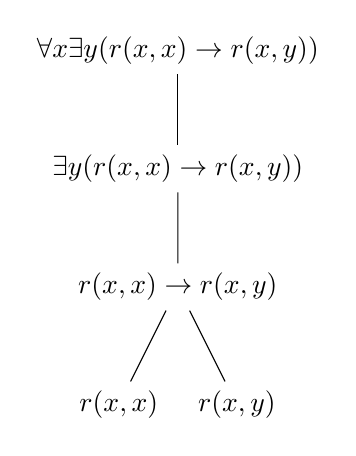
\begin{tikzpicture}[level distance=1.5cm,
  level 1/.style={sibling distance=3cm},
  level 2/.style={sibling distance=1.5cm}]
  \node {$\forall x\exists y(r(x,x)\to r(x,y))$}
    child {node {$\exists y(r(x,x)\to r(x,y))$}
      child {node {$r(x,x)\to r(x,y)$}
        child {node {$r(x,x)$}}
        child {node {$r(x,y)$}}}};
\end{tikzpicture}

\noindent The bottom nodes must each be elementary formulas, i.e.\
either $\bot$, or a relation symbol followed by the appropriate number
of terms.  Each parent-child relationship in the tree corresponds to
one of the Boolean connectives or to one of the quantifiers.

Formulas stand in one-to-one correspondence with parse trees: each
well-formed tree ends with a specific formula, and no other tree
yields the same formula.  Using the identity of formulas and parse
trees, we can easily define a few further helpful notions:

\begin{defn} Let $\vp$ be a $\Sigma$-formula.  The family of
  \textbf{subformulas} of $\vp$ consists of all those formulas that
  occur at some node in its parse tree.  \end{defn}

\begin{defn} If a quantifier $\exists x$ occurs in the formula $\vp$,
  then the \textbf{scope} of that occurrence is the formula which
  occurs at the immediately previous node in the parse
  tree.  \end{defn}

For example, in the formula $\forall x\exists y(r(x,x)\to r(x,y))$,
the scope of $\exists y$ is the formula $r(x,x)\to r(x,y)$.  In
contrast, in the formula $\forall x(r(x,x)\to \exists yr(x,y))$, the
scope of $\exists y$ is the formula $r(x,y)$.

We can now make the notion of free and bound variables even more
precise.  In particular, each individual occurrence of a variable in
$\vp$ is either free or bound.  For example, in the formula
$p(x)\wedge \exists xp(x)$, $x$ occurs freely in the first subformula,
and bound in the second subformula.

\begin{defn}[Free and bound occurrences] An occurence of a variable
  $x$ in $\vp$ is \textbf{bound} just in case that occurrence is
  within the scope of either $\forall x$ or $\exists x$.  Otherwise
  that occurence of $x$ is free. \end{defn}

We could now perform a sanity check to make sure that our two notions
of bound/free variables coincide with each other.

\begin{fact} A variable $x$ is free in $\vp$ (in the sense of the
  definition of $\Sigma$-formulas) if and only if there is a free
  occurence of $x$ in $\vp$ (in the sense that this occurence does not
  lie in the scope of any corresponding quantifier).  \end{fact}


It is also sometimes necessary to distinguish particular occurrences
of a subformula of a formula, and to define the \textbf{depth} at
which such an instance occurs.

\begin{defn} Let $\psi$ be a node in the parse tree of $\vp$.  The
  \textbf{depth} of $\psi$ is the number of steps from $\psi$ to the
  root node.  We say that $\psi$ is a \textbf{proper subformula} of
  $\vp$ if $\psi$ occurs with depth greater than $0$. \end{defn}

The parse trees of formulas are finite, by definition.  Therefore, the
depth of every occurrence of a subformula of $\vp$ is some finite
number.

There are a number of other properties of formulas that are definable
in purely syntactic terms.  For example, we could define the
\textbf{length} of a formula.  We could then note that the connectives
take formulas of a certain length and combine them to create formulas
of a certain greater length.

\begin{exercise} Show that no $\Sigma$-formula can occur as a proper
  subformula of itself. \end{exercise}

% We can give a more precise definition of the structure of a
% $\Sigma$-formula by making use of the notion of a \emph{list} of
% formulas.

% \begin{defn} The family of \emph{lists} of formulas is defined by the
%   following conditions:
%   \begin{enumerate}
%   \item If $\vp _1,\dots ,\vp _n$ are formulas, then
%     $\langle \vp _1 , \cdots , \vp _n\rangle$ is a list.
%   \item If $\sigma _1,\dots ,\sigma _n$ are either formulas or lists
%     of formulas, then $\langle \sigma _1 , \cdots ,\sigma _n\rangle$
%     is a list. \end{enumerate}
% \end{defn}

% A typical list of formulas looks something like this:
% \[ \langle \vp _1 ,\langle \vp _2 ,\vp _1 \rangle ,\vp _3 \rangle .\]
% We are especially interested in lists of formulas such as:
% \[ \langle \vp _1\wedge \vp _2,\langle \vp _1\rangle ,\langle \vp
%   _2\rangle \rangle .\] Here the first item is a Boolean combination,
% the second item is a list with one entry (the first conjunct), and the
% third item is a list with one entry (the second conjunct).

% \begin{defn} Given a list $\sigma$, we let $\sigma _i$ denote the
%   $i$-th entry.  Note that $\sigma _i$ could be another list, or it
%   could be a formula. \end{defn}

% \begin{defn} We define the family of \emph{f-lists} of formulas as
%   follows: \begin{enumerate}
%   \item If $\vp$ is an atomic formula, then $\langle\vp\rangle$ is an
%     f-list.
%   \item If $\sigma$ and $\tau$ are f-lists such that $\sigma _1$ and
%     $\tau _1$ are formulas, then
%     $\langle \sigma _1\wedge \tau _1,\sigma ,\tau \rangle$ is an
%     f-list.
%   \item Similar clauses for the other Boolean connectives.    
%   \item If $\sigma$ is an f-list such that $\sigma _1$ is a formula,
%     then $\langle \forall x\sigma _1 ,\sigma \rangle$ is an f-list.
%   \item A similar clause for $\exists x$.
%   \end{enumerate}
%   \end{defn}

%   \begin{prop} There is a one-to-one correspondence between formulas
%     and f-lists of formulas.  In particular, for each formula $\vp$,
%     there is a unique f-list $\sigma$ such that $\sigma
%     _1=\vp$. \end{prop}

%   \begin{proof} Define a function $f$ from formulas to f-lists
%     by: \begin{enumerate}
%     \item $f(\vp )=\langle\vp\rangle$ for $\vp$ atomic.
%     \item
%       $f(\vp\wedge\psi )=\langle\vp\wedge\psi,f(\vp ),f(\psi
%       )\rangle$, and similarly for the other Boolean connectives.
%     \item $f(\forall x\vp)=\langle\forall x\vp ,f(\vp )\rangle$, and
%       similarly for $\exists x\vp$.
%     \end{enumerate}
%     Then $f(\vp )_1=\vp$, from which it follows that $f$ is injective.

%     We now show that $f$ is surjective, by induction on the
%     construction of f-lists.  Base case: if
%     $\sigma =\langle \vp\rangle$, for $\vp$ an atomic formula, then
%     $\sigma =f(\vp )$.

%         Inductive step: assume that
%         $\sigma = \langle \vp\wedge\vp ',\tau ,\tau '\rangle$, where
%         $\tau$ and $\tau '$ are f-lists in the image of the function
%         $f$.  Let $\tau$ and $\tau '$ be formulas such that
%         $\tau =f(\theta )$ and $\tau '=f(\theta ')$.  By the
%         definition of $f$, $\tau _1=\theta$ and $\tau '_1=\theta '$.
%         By the definition of f-lists, $\vp = \tau _1$ and
%         $\vp '=\tau '_1$.  Thus, $\theta =\vp$ and $\theta '=\vp '$,
%         from which it follows that
%         \[ \sigma \:=\: \langle \vp\wedge\vp',f(\vp ),f(\vp ')\rangle
%           \:=\: f(\vp\wedge \vp ') .\] The remaining inductive steps
%         are similar, and we leave them to the reader.  \end{proof}

%       \begin{disc} In any f-list
%         $\sigma = \langle \vp ,\dots \rangle$, the angle brackets are
%         balanced.  What's more, any formula $\psi$ that occurs in
%         $\sigma$ is surrounded by $n$ pairs $\langle\cdot\rangle$, for
%         some $n\geq 1$.  Then $n-1$ is the \emph{depth} of this
%         occurence of $\psi$ in $\vp$. \end{disc}





% %% Example proofs by induction on construction?

%       [[TO DO: move]] Any time we define a set inductively, we have a
%       corresponding method of proof by induction.  In this case, we
%       can prove that a property $\mathbb{P}$ holds for all
%       $\Sigma$-formulas by showing that $\mathbb{P}$ holds for all
%       elementary $\Sigma$-formulas, and that $\mathbb{P}$ is preserved
%       by the various operations that allow us to construct more
%       complex $\Sigma$-formulas.  What is a bit more difficult in this
%       case is proving that some property holds of all
%       $\Sigma$-sentences, when that property does not hold of all
%       $\Sigma$-formulas.  In such cases, we'll have to look for a
%       clever way to modify the standard sort of proof by induction.


%% TO DO: define the notation $\vp [t/x]$

We now define a substitution operation $\vp\mapsto \vp [t/x]$ on
formulas, where $t$ is a fixed term, and $x$ is a fixed variable.  The
intention here is that $\vp [t/x]$ results from replacing all free
occurrences of $x$ in $\vp$ with $t$.  We first define a corresponding
operation on terms.

\begin{defn} Let $t$ be a fixed term, and let $x$ be a fixed variable.
  We define the operation $s\mapsto s[t/x]$, where $s$ is an arbitrary
  term, as follows:
  \begin{enumerate}
  \item If $s$ is a variable, then $s[t/x]\equiv s$ when
    $s\not\equiv x$, and $s[t/x]\equiv t$ when $s\equiv x$.  (Here
    $\equiv$ means literal identity of strings of symbols.)
  \item Suppose that $s\equiv f(t_1,\dots ,t_n)$, where $f$ is a function
    symbol and $t_1,\dots ,t_n$ are terms.  Then we define 
    \[ s[t/x] \: \equiv \: f(t_1[t/x],\dots ,t_n[t/x]) .\] This
    includes the special case where $f$ is a $0$-ary function symbol,
    where $f[t/x]\equiv f$.
  \end{enumerate}
\end{defn}

\begin{defn} Let $t$ be a fixed term, and let $x$ be a fixed variable.
  We define the operation $\vp\mapsto \vp [t/x]$, for $\vp$ an
  arbitrary formula, as follows:
  \begin{enumerate}
  \item For the proposition $\bot$, let $\bot [t/x]:=\bot$.
  \item For an elementary formula $r(t_1,\dots ,t_n)$, let 
    \[ r(t_1,\dots ,t_n)[t/x] \: := \: r(t_1[t/x],\dots ,t_n[t/x]) .\]
  \item For a Boolean combination $\vp\wedge\psi$, let
    \[ (\vp\wedge\psi )[t/x] \: : = \: \vp [t/x]\wedge \psi [t/x] ,\]
    and similarly for the other Boolean connectives.
  \item For an existentially quantified formula $\exists y\vp$, let
    \[ (\exists y\vp )[t/x] := \left\{ \begin{array}{l l} \exists y(\vp
                                         [t/x]) & \text{if}\; x\not\equiv y , \\
                                         \exists y\vp & \text{if}\;
                                                        x\equiv y
                                                        .\end{array}
                                                    \right. \]
\item For a universally quantifier formula $\forall y\vp$, let \[ (\forall y\vp )[t/x] := \left\{ \begin{array}{l l}
                                                  \forall y(\vp
                                         [t/x]) & \text{if}\; x\not\equiv y , \\
                                         \forall y\vp & \text{if}\;
                                                        x\equiv y
                                                        .\end{array}
                                                    \right. \]
                                                  
\end{enumerate}
\end{defn}

\begin{prop} For any formula $\vp$, the variable $x$ is not free in
  $\vp [y/x]$. \end{prop}

\begin{proof} We first show that $x\not\in FV(t[y/x])$ for any term
  $t$.  That result follows by a simple induction on the construction
  of terms.

  Now let $\vp$ be an elementary formula.  That is,
  $\vp =r(t_1,\dots ,t_n)$.  Then we have
  \[ \begin{array}{l l l} FV(\vp [y/x]) & = & FV(r(t_1,\dots ,t_n)[y/x]) \\
                                        &=& FV(r(t_1[y/x],\dots ,t_n[y/x])) \\
                                        &=& FV(t_1[y/x])\cup\cdots\cup
                                            FV(t_n[y/x])
                                            .\end{array} \] %%
                                        Since $x\not\in FV(t_i[y/x])$,
                                        for $i=1,\dots ,n$, it follows
                                        that $x\not\in FV(\vp [y/x])$.

The argument for the Boolean connectives is trivial, so we turn to the
argument for the quantifiers.  Suppose that the result is true for
$\vp$.  We need to show that it's also true for $\exists v\vp$.
Suppose first that $v\equiv x$.  In this case we have
\[ (\exists v\vp )[y/x] = (\exists x\vp )[y/x] = \exists x\vp .\]
Since $x\not\in FV(\exists x\vp )$, it follows that $x\not\in
FV((\exists v \vp )[y/x])$.  Suppose now that $v\not\equiv x$.  In
this case we have
\[ (\exists v\vp )[y/x] = \exists v(\vp [y/x]) .\] Since
$x\not\in FV(\vp [y/x])$, it follows then that
$x\not\in FV((\exists v\vp )[y/x])$. The argument is analogous for the
quantifier $\forall v$.  Therefore, for any formula $\vp$, the
variable $x$ is not free in $\vp [y/x]$.
\end{proof}




%% Things still to prove

%% 1. Substitution in the formula
%% \vp \vdash \psi -- can switch out the free variables

%% 2. Alpha equivalence





\section{Deduction rules}

We suppose again that $\Sigma$ is a fixed signature.  The goal now is
to define a relation $\Gamma \vdash \vp$ of derivability, where
$\Gamma$ is a finite sequence of $\Sigma$-formulas, and $\vp$ is a
$\Sigma$-formula.  Our derivation rules come in three groupings: rules
for the Boolean connectives, rules for the $\bot$ symbol, and rules
for the quantifiers.

\subsection*{Boolean connectives}

We carry over all of the rules for the Boolean connectives from
propositional logic (see Section \ref{sec:pt}).  These rules require
no special handling of variables.  For example, the following is a
valid instance of $\wedge$-elim:
\[ \begin{array}{l}
     \Gamma \RA \vp (x)\wedge \psi (y) \\
     \hline \Gamma \RA \vp (x) \end{array} \]

\subsection*{Falsum} 

We intend for the propositional constant $\bot$ to serve as shorthand
for ``the false.''  To this end, we define its introduction and
elimination rules as follows.

\bigskip \begin{tabular}{c c c } \begin{tabular}{|l l |} \hline \textbf{$\bot$ intro}
    & \begin{tabular}{l}
        $\Gamma \RA \vp\wedge \neg \vp$ \\
        \hline $\Gamma \RA \bot $ \end{tabular} \\
                    \hline \end{tabular}
& & \begin{tabular}{|l l |} \hline  \textbf{$\bot$ elim} & \begin{tabular}{l}
                                             $\Gamma \RA \bot $  \\
                                             \hline $\Gamma \RA \vp
                                             $ \end{tabular} \\
                    \hline \end{tabular} \end{tabular}



\subsection*{Quantifiers}

In order to formulate good derivation rules for the quantifiers, we
have to make a couple of strategic choices.  In actual mathematical
practice, mathematicians simply introduce new vocabulary whenever they
need it.  In some cases, new vocabulary is introduced by way of
definition --- for example, when a mathematician says something like,
``we say that a number $x$ is \textit{prime} just in case \dots '',
where the words following the dots refer to previously understood
mathematical concepts.  In other cases, the newly introduced
vocabulary is really just newly introduced notation --- for example,
when a mathematician says something like, ``let $n$ be a natural
number.''  In this latter case, the letter ``$n$'' wasn't a part of
the original vocabulary of the theory of arithmetic, and was
introduced as a matter of notational convenience.

Nonetheless, for our purposes it will be most convenient to have a
fixed vocabulary $\Sigma$ for a theory.  But this means that if
$\Sigma$ has no constant symbols, then we might have trouble making
use of the quantifier introduction and elimination rules.  For
example, imagine trying to derive a theorem in the theory of Boolean
algebras is you weren't permitted to say, ``let $a$ be an arbitrary
element of the Boolean algebra $B$.''  In order to simulate
mathematics' free use of new notation, we'll simply be a bit more
liberal in the way that we allow free variables to be used.  To this
end, we define the following notion:

\begin{defn} We say that \emph{$t$ is free for $x$ in $\vp$} just in
  case one of the following conditions holds:
  \begin{enumerate}
  \item $\vp$ is atomic, or
  \item $\vp$ is a Boolean combination of formulas, in each of which
    $t$ is free for $x$, or
  \item $\vp:=\exists y\psi$, and $y\not\in FV(t)$, and $t$ is free
    for $x$ in $\psi$, where $x\neq y$. \end{enumerate} \end{defn}

Intuitively speaking, $t$ is free for $x$ in $\vp$ just in case
substituting $t$ in for $x$ in $\vp$ does not result in any of the
variables in $t$ being captured by quantifiers.  For example, in the
formula $p(x)$, the variable $y$ is free for $x$ (since $y$ is free in
$p(y)$).  In contrast, in the formula $\exists yp(x)$, the variable
$y$ is not free for $x$ (since $y$ is not free in $\exists yp(y)$).
We will need this notion in order to coordinate our intro and elim
rules for the quantifiers.  For example, the rule of $\forall$-elim
should say something like: $\forall x\vp (x)\vdash \vp (y)$.  However,
if this rule were not restricted in some way, then it would yield
\[ \forall x\exists y(x\neq y) \: \vdash \: \exists y(y\neq y) ,\]
which is intuitively invalid.

\begin{figure}[H]
\begin{tabular}{|l l l|}
  \hline  \textbf{$\forall$ intro}
  & \makecell[l]{ $\Gamma \: \vdash \:
    \vp$ \\ \hline $\Gamma \: \vdash \: \forall x\vp$ }
  & \makecell[l]{\small where $x$ is not free in $\Gamma$.}  \\ \hline \end{tabular}

\bigskip \begin{tabular}{|l l l|} \hline 
  \textbf{$\forall$ elim} & \makecell[l]{
                            $\Gamma \: \vdash \: \forall x\vp$ \\ \hline
  $\Gamma \: \vdash \: \vp [t/x]$ } & \makecell[l]{\small where $t$
                                      is free for $x$.} \\ \hline
\end{tabular} \end{figure}

The $\forall$-intro rule is easy to apply, for we only need to check
that the variable $x$ doesn't occur in the assumptions $\Gamma$ from
which $\vp$ is derived.  Note that application of the $\forall$-intro
rule can result in empty quantification; so example,
$\forall x\forall xp(x)$ follows from $\forall xp(x)$.

To understand the restrictions on $\forall$-elim, note that it does
license
\[ \forall x\, r(x,x) \: \vdash \: r(y,y) , \]
since $r(x,x)[y/x]\equiv r(y,y)$.  In contrast, $\forall$-elim does not license
\[ \forall x\,r(x,x) \: \vdash \: r(x,y) , \] since it is not the case
that $r(x,x)[y/x]\equiv r(x,y)$.  Similarly, $\forall$-elim does not
license
\[ \forall x\exists y\,r(x,y) \: \vdash \: \exists y\,r(y,y) ,\] since
$y$ is not free for $x$ in $\exists y\,r(x,y)$.  Finally,
$\forall$-elim permits universal quantifiers to be peeled off when
they don't bind any variables.  For example, $\forall x\,p\vdash p$ is
licensed by $\forall$-elim.

Now we turn to the rules for the existential quantifier.  First we
state the rules in all their sequential glory:

\begin{figure}[H]
  \begin{tabular}{|l l l|} \hline \textbf{$\exists$ intro} &
    \makecell[l]{ $\Gamma \: \vdash \: \vp [t/x]$ \\ \hline
      $\Gamma \: \vdash \: \exists x\vp $ } & \makecell[l]{\small
      provided $t$ is
                                              free for $x$ in $\vp$.} \\
                                              \hline \end{tabular}

\bigskip \begin{tabular}{|l l l|} \hline 
    \textbf{$\exists$ elim} & \makecell[l]{
                             $\Gamma ,\vp \:\vdash \: \psi $ \\
    \hline $\Gamma ,\exists x\vp \: \vdash \: \psi$ } &
                                                        \makecell[l]{\small
                                                        provided $x$
                                                        is not free in
                                                        $\psi$ or
                                                        $\Gamma$.}  \\
    \hline \end{tabular} \end{figure}

If we omit the use of auxiliary assumptions, we can rewrite the
$\exists$ rules as follows:

\begin{figure}[H]
  \begin{tabular}{|l l l|} \hline \textbf{$\exists$ intro} &
\makecell[l]{ $\vdash \: \vp [t/x]$ \\ \hline
      $\vdash \: \exists x\vp $ } & {\small
                                                    provided $t$ is
                                                      free for $x$ in $\vp$.}
    \\ \hline \end{tabular}

\bigskip \begin{tabular}{|l l l|} \hline 
\textbf{$\exists$ elim} & \makecell[l]{
                              $\vp \:\vdash \: \psi $ \\
    \hline $\exists x\vp \: \vdash \: \psi$ } &
                                                            \makecell[l]{\small
                                                            provided $x$
                                                            is not
                                                            free in
                                                            $\psi$.}
    \\ \hline \end{tabular} \end{figure}

Again, let's look at some examples to illustrate the restrictions.
First, in the case of the $\exists$-intro rule, suppose that there
were no restriction on the term $t$.  Let $\vp$ be the formula
$\forall y\,r(x,y)$, and let $t$ be the variable $y$, in which case
$\vp [t/x]\equiv \forall y\,r(y,y)$.  Then the $\exists$-in rule would
yield
\[ \forall y\,r(y,y) \: \vdash \: \exists x\forall y\,r(x,y ), \]
which is intuitively invalid.  (Consider, for example, the case where
$r$ is the relation $\leq$ on integers.)  The problem, of course, is
that the variable $y$ is captured by the quantifier $\forall y$ when
substituted into $\vp$.  Similarly, in the case of the $\exists$-elim
rule, if there were no restriction on the variable $x$, then we could
derive $\vp$ from $\exists x\vp$, and then using $\forall$-intro, we
could derive $\exists x\vp\vdash \forall x\vp$.

\subsection*{Structural rules}

In any proof system, there are some more or less tacit rules that
arise from how the system is set up.  For example, when someone learns
natural deduction, e.g.\ via the system presented in Lemmon's {\it
  Beginning Logic}, then she will tacitly assume that she's allowed to
absorb dependencies, e.g.\ if $\phi ,\phi\vdash \psi$ then
$\phi \vdash \psi$.  These more or less tacit rules are called
\emph{structural rules} of the system --- and there is a lot of
interesting research on logical systems that drop one or more of these
structural rules \cite[see][]{restall}.  In this book, we stay within
the confines of classical first-order logic; and we will not need to
be explicit about the structural rules, except for the rule of
\emph{cut}, which allows sequents to be combined.  Loosely speaking,
cut says that if you have sequents $\Gamma \vdash \phi$ and
$\Delta ,\phi\vdash \psi$, then you may derive the sequent
$\Gamma ,\Delta \vdash \psi$.

As was the case with propositional logic, we will not specify a
canonical way of writing predicate logic proofs.  After all, our goal
here is not to teach you the art of logical deduction; rather, our
goal is to reflect on the relations between theories in formal logic.


\subsection*{Equality}

As we mentioned before, there's something of a philosophical debate
about whether the equality symbol $=$ should be considered as part of
the logical or the non-logical vocabulary of a theory.  We don't want
to get tangled up in that argument, but we do wish to point out how
the axioms for equality compare to the axioms for a generic
equivalence relation.

It is typical to write down two axioms for equality, an introduction
and an elimination rule.  Equality introduction permits $\vdash t=t$
with any term $t$.  Equality elimination permits
\[ \begin{array}{c c} t=s \quad \vp [t/s] \\ \hline \vp
   \end{array} \] so long as $t$ is free for $s$ in $\vp$.  Note that equality elimination allows us to
 replace single instances of a term.  For example, if we let $\vp$
 be the formula $r(s,t)$, then $\vp [t/s]$ is the formula $r(t,t)$.
 Hence from $t=s$ and $r(t,t)$, equality elimination permits us to
 derive $r(s,t)$.

 From the equality axioms, we can easily show that it's an equivalence
 relation.  The introducton rule shows that it's reflexive.  For
 symmetry, we let $\vp$ be the formula $y=x$, in which case
 $\vp [x/y]$ is the formula $x=x$.  Thus, we have
   \[ \begin{array}{c c} x=y\quad x=x \\ \hline y=x \end{array} \]
   For transitivity, let $\vp$ be the formula $x=z$, in which case
   $\vp [y/x]$ is the formula $y=z$.  Thus, we have
   \[ \begin{array}{c c} y=x\quad y=z \\ \hline x=z \end{array} \]

   This completes the list of the proof rules for our system of
   first-order logic, i.e.\ our definition of the relation $\vdash$.
   Before proceeding to investigate the properties of this relation,
   let's see a couple of examples of informal proofs.

   \begin{example} Let's show that
     $\exists x(\vp (x)\wedge \psi (x))\vdash \exists x\vp (x)$.
     First note that $\vp (x)\wedge \psi (x)\vdash \vp (x)$ from
     $\wedge$-elim.  Then
     $\vp (x)\wedge \psi (x)\vdash \exists x\vp (x)$ from
     $\exists$-intro.  Finally, since $\exists x\vp (x)$ contains no
     free occurrences of $x$, we have
     $\exists x(\vp (x)\wedge \psi (x))\vdash \exists x\vp
     (x)$.  \end{example}

   \begin{example} Of course we should have
     $\forall x\vp \vdash \forall y(\vp [y/x])$, so long as $y$ is
     free for $x$ in $\vp$.  Using the rules we have, we can derive
     this result in two steps.  First, we have
     $\forall x\vp (x)\vdash \vp [y/x]$ from $\forall$-elim, and then
     $\vp [y/x]\vdash \forall y\vp [y/x]$ by $\forall$-intro.  We only
     need to verify that $x$ is not free in $\vp [y/x]$.  This can be
     shown by a simple inductive argument.   \end{example}

% \begin{prop} For any formula $\vp$, the variable $x$ is not free in
%   $\vp [y/x]$. \end{prop}

% \begin{proof} We first show that $x\not\in FV(t[y/x])$ for any term
%   $t$.  That result follows by a simple induction on the construction
%   of terms.

%   Now let $\vp$ be an elementary formula.  That is,
%   $\vp =r(t_1,\dots ,t_n)$.  Then we have
%   \[ \begin{array}{l l l} FV(\vp [y/x]) & = & FV(r(t_1,\dots ,t_n)[y/x]) \\
%                                         &=& FV(r(t_1[y/x],\dots ,t_n[y/x])) \\
%                                         &=& FV(t_1[y/x])\cup\cdots\cup
%                                             FV(t_n[y/x])
%                                             .\end{array} \] %%
%                                         Since $x\not\in FV(t_i[y/x])$,
%                                         for $i=1,\dots ,n$, it follows
%                                         that $x\not\in FV(\vp [y/x])$.

% The argument for the Boolean connectives is trivial, so we turn to the
% argument for the quantifiers.  Suppose that the result is true for
% $\vp$.  We need to show that it's also true for $\exists v\vp$.
% Suppose first that $v\equiv x$.  In this case we have
% \[ (\exists v\vp )[y/x] = (\exists x\vp )[y/x] = \exists x\vp .\]
% Since $x\not\in FV(\exists x\vp )$, it follows that $x\not\in
% FV((\exists v \vp )[y/x])$.  Suppose now that $v\not\equiv x$.  In
% this case we have
% \[ (\exists v\vp )[y/x] = \exists v(\vp [y/x]) .\] Since
% $x\not\in FV(\vp [y/x])$, it follows then that
% $x\not\in FV((\exists v\vp )[y/x])$. The argument is analogous for the
% quantifier $\forall v$.  Therefore, for any formula $\vp$, the
% variable $x$ is not free in $\vp [y/x]$.
% \end{proof}


%% TO DO: talk about Tarski point -- that theories aren't closed just
%% under deduction, but also conceptually, i.e. by taking definitions
%% TO DO: a philosophical reflection on definition

Recall that propositional logic is compositional in the following
sense: Suppose that $\vp$ is a formula, and $\psi$ is a subformula of
$\vp$.  Let $\vp '$ denote the result of replacing $\psi$ in $\vp$
with another formula $\psi '$ where
$\vdash \psi\leftrightarrow \psi '$.  Then
$\vdash \vp\leftrightarrow \vp '$.  That result is fairy easy to prove
by induction on the construction of proofs.  It also follows from the
truth-functionality of the Boolean connectives, by means of the
completeness theorem.  In this section, we are going to prove an
analogous result for predicate logic.  To simplify notation, we
introduce the following:

\begin{defn} For formulas $\vp$ and $\psi$, we say that $\vp$ and
  $\psi$ are \emph{logically equivalent}, written $\vp\simeq\psi$,
  just in case both $\vp\vdash\psi$ and $\psi\vdash\vp$.
\end{defn}

It is not hard to show that $\simeq$ is an equivalence relation on the
set of formulas.  Note that formulas $\vp$ and $\psi$ can be
equivalent in this sense even if they don't share all free variables
in common --- as long as the non-matching variables occur vacuously.
For example, $p(x)$ is equivalent to $p(x)\wedge (y=y)$, and it's also
equivalent to $p(x)\vee (y\neq y)$.  [The issue here has nothing in
particular to do with the equality relation.  The variable $y$ also
occurs vacuously in $p(y)\vee \neg p(y)$.]  In contrast, the formulas
$p(x)$ and $p(y)$ are not equivalent (in the empty theory), since it's
not universally valid that
$\vdash \forall x\forall y(p(x)\leftrightarrow p(y))$.

\begin{lemma} The relation $\simeq$ is compatible with the Boolean
  connectives in the following sense: if $\phi\simeq\phi '$ and
  $\psi\simeq \psi '$, then
  $(\phi\wedge \psi )\simeq (\phi '\wedge \psi ')$, and similarly for
  the other Boolean connectives. \end{lemma}

The proof of this lemma is a fairly simple application of the
introduction and elimination rules for the connectives.  To complete
the proof of the replacement theorem, we need one more lemma.

\begin{lemma} If $\vp\simeq \psi$ then
  $\exists x\vp\simeq \exists x\psi$. \end{lemma}

\begin{proof} Suppose that $\vp\simeq\psi$, which means that
  $\vp\vdash \psi$ and $\psi\vdash \vp$.  We're now going to show that
  $\exists x\vp\vdash\exists x\psi$.  By $\exists$-in we have
  $\psi\vdash \exists x\psi$, hence by cut we have
  $\vp\vdash\exists x\psi$.  Since $x$ does not occur free in
  $\exists x\psi$, we have $\exists \vp\vdash \exists x\psi$ by
  $\exists$-out.  \end{proof}

%% TO DO: fix this
\begin{thm}[Replacement] Suppose that $\vp$ is a formula in which
  $\psi$ occurs as a subformula, and $\vp '$ is the result of
  replacing $\psi$ with $\psi '$.  If $\psi \simeq \psi '$ then
  $\vp \simeq \vp '$.
\end{thm}

In most presentations of the predicate calculus (i.e.\ the definition
of the relation $\vdash$) the two central results are the soundness
and completeness theorems.  Intuitively speaking, the soundness
theorem shows that the definition doesn't overgenerate, and the
completeness theorem shows that it doesn't undergenerate.  However, in
fact, these results show something quite different --- they show that
the definition of $\vdash$ matches the definition of another relation
$\vDash$.  We will discuss this other relation $\vDash$ in Chapter
\ref{chap-sem}, where we will also prove the traditional soundness and
completeness theorems.  In the remainder of this section, we show that
the predicate calculus is consistent in the following purely syntactic
sense.

\begin{defn} We say that the relation $\vdash$ is \emph{consistent}
  just in case there is some formula $\phi$ that is not provable.
  Similarly, we say that a theory $T$ is \emph{consistent} just in
  case there is a formula $\phi$ such that
  $T\not\vdash\phi$. \end{defn}

Note that the definition of consistency for $\vdash$ presupposes a
fixed background signature $\Sigma$.

\begin{prop} A theory $T$ is consistent iff
  $T\not\vdash\bot$.  \end{prop}

\begin{proof} If $T$ is inconsistent then $T\vdash\phi$ for all
  formulas $\phi$.  In particular, $T\vdash \bot$.  Conversely, if
  $T\vdash\bot$, then RA and DN yield $T\vdash\phi$ for any formula
  $\phi$. \end{proof}

%% TO DO: here I should have the van Dalen proof

\begin{thm} The predicate calculus is consistent. \end{thm}

%% TO DO: I would like to inspect this theorem more closely.  
\begin{proof} Let $\Sigma$ be a fixed predicate logic signature, and
  let $\Sigma '$ be a propositional signature whose cardinality is
  greater than or equal to that of $\Sigma$.  We will use the symbol
  $\vdash ^*$ to denote derivability in the propositional calculus.
  Define a map $\vp\mapsto\vp ^*$ from the formulas of $\Sigma$ to the
  formulas of $\Sigma '$ as follows:
\begin{itemize}
\item $\bot ^*=\bot$
\item For any terms $t_1,\dots ,t_n$,
  $(p_i(t_1,\dots ,t_{n_i}))^*=q_i$.
\item $(\vp\wedge\psi )^*=\vp ^*\wedge \psi ^*$, and similarly for the
  other Boolean connectives.
\item $(\forall x\vp )^*=\vp ^*$ and $(\exists x\vp )^*=\vp ^*$.
\end{itemize}
We now use induction on the definition of $\vdash$ to show that if
$\Gamma\vdash\vp$ then $\Gamma ^*\vdash ^*\vp ^*$.  We will provide a
few representative steps, and leave it to the reader to supply the
others.

\begin{itemize}
\item The base case, rule of assumptions, is trivial.
\item Consider the case of $\wedge$-out.  Suppose that
  $\Gamma\vdash\vp$ follows from $\Gamma\vdash\vp\wedge\psi$ by
  $\wedge$-out.  By the inductive hypothesis,
  $\Gamma ^*\vdash ^*(\vp\wedge\psi )^*$.  Using the definition of
  $(\vp\wedge\psi )^*$, it follows that
  $\Gamma ^*\vdash ^*\vp ^*\wedge \psi ^*$.  Hence by $\wedge$-out, we
  have $\Gamma ^*\vdash ^* \vp ^*$.
\item Consider the case of $\forall$-in.  That is, suppose that
  $\Gamma\vdash\forall x\vp$ is derived from $\Gamma\vdash\vp$ using
  $\forall$-in.  In this case, the induction hypothesis tells us that
  $\Gamma ^*\vdash ^*\vp ^*$.  And since $(\forall x\vp )^*=\vp ^*$,
  we have $\Gamma ^*\vdash ^*(\forall x\vp )^*$.
\end{itemize}
Completing the previous steps shows that if $\Gamma\vdash\vp$ then
$\Gamma ^*\vdash ^*\vp ^*$.  Since the propositional calculus is
consistent, $\not\vdash ^*\bot$, and therefore
$\not\vdash\bot$. \end{proof}

\begin{disc} Notice that the previous proof does not use the fact that
  our $\forall$-intro rule demands that $x$ not occur free in
  $\Gamma$.  Thus, this proof also shows the consistency of a proof
  system with an \textit{unrestricted} $\forall$-in rule.

  But an unrestricted $\forall$-intro rule would nonetheless severely
  restrict the expressive power of our logic.  Indeed, it would
  license
  \[ x\neq y \: \vdash \: \forall y(x\neq y) \: \vdash \: x\neq x , \]
  the last of which contradicts the axioms for equality.  Thus, an
  unrestricted $\forall$-intro would make $\forall x\forall y(x=y)$ a
  tautology. 
\end{disc}





\section{Empirical theories} \label{sec:et}

%% TO DO: Carnap's various attempts to connect theoretical terms with
%% observation language

%% TO DO: here is place to discuss question of whether FOL is too
%% restrictive.  versus "theories in the wild".

%% original Carnap proposal .... and how it was eviscerated by van
%% Fraassen etc.

Here we use the phrase ``empirical theory'' or ``scientific theory'',
to mean a theory that one intends to describe the physical world.  You
know many examples of such theories: Newtonian mechanics, Einstein's
general theory of relativity, quantum mechanics, evolutionary biology,
the phlogiston theory of combustion, etc..  You may also know many
examples of theories from pure mathematics, such as set theory, group
theory, ring theory, topology, and the theory of smooth manifolds.
Intuitively, empirical theories differ in some important way from pure
mathematical theories.  We stress ``intuitively'' here because Quine
brought into question the idea that there is a principled distinction
between two types of theories.  For the time being, we won't engage
directly with Quine's more philosophical arguments against this
distinction.  Instead, we will turn back the clock to the time when
Rudolf Carnap, among others, hoped that formal logic might illuminate
the structure of scientific theories.

Rudolf Carnap was the primary advocate of the idea that philosophers
ought to pursue a {\it syntactic} analysis of scientific theories.
The story is typically told as follows: Carnap sought to construct a
theory {\it of} scientific theories.  Moreover, following in the
footsteps of Bertrand Russell and Gottlob Frege, Carnap believed that
philosophy had no business directly engaging in empirical questions.
As \cite{russ} had argued, philosophers ought to leave empirical
questions to the empirical sciences.  Thus, Carnap thought that a good
philosophical theory of scientific theories ought to restrict itself
to the purely formal aspects of those theories.  In particular, the
``metascientist'', i.e.\ the philosopher of science, ought to make use
only of syntactic concepts.

Carnap begins his {\it Wissenschaftslogik} program in earnest in his
first major book, {\it Logische Aufbau der Welt}.  Already here we see
the emphasis on ``explication'', i.e.\ of taking an intuitive concept,
and providing a precise formal counterpart.  Carnap's paradigms of
explication are those from 19th and early 20th century mathematics ---
explications of concepts such as ``infinity'' and ``continuous
function'' and ``open subset''.  Nonetheless, in the {\it Aufbau},
Carnap hasn't yet found his primary tool of analysis.  That would only
come from the development, in the 1920s, of logical metatheory.
Carnap was working at the time in Vienna, among the other members of
the infamous Vienna Circle.  One of the youngest members of the circle
was Kurt G{\"o}del, whose 1929 PhD thesis contained the first proof of
the completeness of the predicate calculus.  Thus, logical metatheory
--- or metamathematics --- was in the air in Vienna, and Carnap was to
try his hand at applying an analogous methodology to the empirical
sciences.  As the goal of metamathematics is to provide a rigorous
theory {\it about} mathematics, Carnap wished to create a rigorous
theory {\it about} the empirical sciences.

By the mid 1930s, Carnap had found his vision.  In {\it Die Logische
  Syntax der Sprache}, Carnap states that his goal is to formalize
scientific theories in the same way that Russell and Whitehead had
formalized arithmetic --- but with one important addition.  With a
theory of pure mathematics, the job is done once the relevant
primitive concepts and axioms have been written down.  However,
empirical theories are, by their nature, ``world directed'', i.e.\
they try to say something about concrete realities.  Thus, an adequate
analysis of a scientific theory cannot rest content with explaining
that theory's formal structure.  This analysis must also say something
about how the theory gains its {\it empirical content}.

The task of explaining how a theory gains empirical content was to
occupy Carnap for most of the remainder of his career.  In fact, it
became the stone on which the entire logical positivist movement
stumbled.  But we've gotten ahead of ourselves.  We need first to see
how Carnap proposed to analyze the structure of empirical theories.

What then is a theory?  From the point of view of first-order logic, a
theory $T$ is specified by a signature $\Sigma$, and a set of axioms
in that signature.  Amazingly, many of the theories of pure
mathematics can be described in terms of this simple schema.  If,
however, we intend for our theory $T$ to describe concrete reality,
what more do we need to add?  Carnap's first proposal was a blunt
instrument: he suggests to identify the empirical content of a theory
by means of a division of that theory's vocabulary into two parts:
\begin{quote}
  The total language of science, $L$, is considered as consisting of
  two parts, the observation language $L_O$ and the theoretical
  language $L_T$. \dots Let the observation vocabulary $V_O$ be the
  class of the descriptive constants of $L_O$. \dots The terms of
  $V_O$ are predicates designating observable properties of events or
  things (e.g., ``blue,'' ``hot,'' ``large,'' etc.) or observable
  relations between them (e.g., ``$x$ is warmer than $y$,'' ``$x$ is
  contiguous to $y$,'' etc.). \citep[pp.\ 40-41]{carnap-met}
\end{quote}
Let's rewrite all of this in a better notation: the language of
science consists of all the formulas built on some particular
signature $\Sigma$, where $\Sigma$ has a subset $O\subseteq \Sigma$ of
observation vocabulary.  The idea here is that terms in $O$ have
ostensive definitions, e.g.\ $O$ might contain predicates such as
``$x$ is red'', or ``$x$ is to the left of $y$''.  The elements of
$\Sigma\backslash O$ are theoretical vocabulary, which need not have
any direct empirical meaning.  For example, $\Sigma\backslash O$ might
contain predicates such as ``$x$ is a force''.  Thus, Carnap hopes to
isolate empirical content by means of specifying a preferred
subvocabulary of the language of science.

Before proceeding, note that Carnap --- in this 1956 article ---
explicitly states that, ``for each language part the admitted types of
variables are specified.''  That phrase was completely ignored by
Carnap's subsequent critics, as we will soon see.  And why did they
ignore it?  The reason, we suspect, is that they had been convinced by
Quine that the notion of ``types of variables'' couldn't possibly make
any difference in any philosophical debate.  Well, Quine wasn't
exactly right about that, as we discuss in Section \ref{quine-sort}.
However, at present our goal is to see Carnap through the eyes of his
critics, and according to these critics, Carnap's proposal amounts to
saying that:

\begin{defn} A formula $\vp$ of $\Sigma$ is an \emph{observation
    formula} (alternatively, \emph{protocol sentence}) just in case no
  symbol in $\vp$ comes from $\Sigma \backslash O$.  If $T$ is a
  theory in $\Sigma$, then we let $T|_O$ denote all the consequences
  of $T$ in the sublanguage based on $O$.  \end{defn}

In the light of these definitions, Carnap's proposal would amount to
saying that the \emph{empirical content} of a theory $T$ is $T|_O$.
Indeed, that's precisely what people took him to be saying --- and
they judged him accordingly.  In fact, one of the standard
``challenges for scientific realism'' was to point out that the
empirical subtheory $T|_O$ has the same empirical content as the
original theory $T$.  Thus, every non-trivial theory $T$ has an
empirically equivalent rival!  

\begin{defn} Let $T_1$ and $T_2$ be theories in $\Sigma$.  Then $T_1$
  and $T_2$ have the same empirical content, i.e.\ are
  \emph{empirically equivalent}, just in case
  $T_1|_O=T_2|_O$.  \end{defn}

This definition fits right in with the picture that the logical
positivists treat sentences as synonymous whenever those sentences
have the same empirical content.  Indeed, many people take the
positivists to be saying that two scientific theories $T_1$ and $T_2$
should be considered equivalent {\it tout court} if they have the same
observational consequences.

Before we go on to consider the criticisms that were brought against
Carnap's picture of empirical content, let's ask ourselves what
purpose the picture was supposed to serve.  In other words, what
questions was Carnap trying to answer by means of this proposal?  In
fact, it seems that Carnap was trying to answer several questions
simultaneously.  First, Carnap, along with many other logical
positivists, was concerned with epistemological questions, such as,
``am I justified in believing theory $T$?''  Apropos of this question,
the goal of isolating empirical content is to make some headway on
understanding how it is that we can be warranted in believing a
theory.  To be clear, it's not only empiricists who should want to
understand how we can use evidence to regulate our belief in a theory.
That's a problem for anyone who thinks that we can learn from
experience --- and that's everybody besides the most extreme
rationalists.

Nonetheless, there were some logical positivists --- and perhaps
sometimes Carnap himself --- who thought that the empirical content of
a theory provides the {\it only} route to justifying belief in that
theory.  For that kind of radical empiricist, isolating empirical
content takes on an additional negative role: of showing which parts
of a theory do {\it not} contribute to our reasons for believing (or
accepting) it.

It is sometimes forgotten, however, that epistemology was not the only
reason that Carnap wanted to isolate empirical content.  In fact,
there are good reasons to think that epistemology wasn't even the
primary reason that Carnap wanted to isolate empirical content.  To
the contrary, Carnap --- who was, by training, a neo-Kantian --- was
concerned with how the abstract, highly mathematical theories of
physics function in making assertions about the world.  To understand
this, we have to remember that Carnap was vividly aware of the
upheaval caused by the discovery, in the mid 19th century, of
non-euclidean geometries.  One result of this upheaval was that
mathematical formalism became {\it detached} from the empirical world,
and the words that occur in it were {\it de-interpreted}.  For
example, in pre-19th century geometry, mathematicians were wont to
think that a word such as ``line'' refers to those things in physical
reality that are, in fact, lines.  But insofar as the word ``line''
occurs in pure geometry, it has no reference at all --- it is merely a
symbol in a formal calculus.

Given the flight of pure mathematics away from empirical reality, the
task the mathematized empirical sciences is to tie mathematics back
down.  In other words, the task of the mathematical physicist is to
take the uninterpreted symbols of pure mathematics, and to endow them
with empirical significance.  It is precisely this methodological
maneuver --- peculiar to the new physics --- that drives Carnap's
desire to analyze the notion of the empirical content of a theory.

In the middle of the 20th century, analytic philosophy moved west ---
from Vienna and Berlin to Oxford, Cambridge (both old and new
England), and then to Princeton, Pittsburgh, UCLA, etc.  As analytic
philosophy moved west, the focus on narrowly epistemological questions
increased.  It's no surprise, then, that Carnap's critics --- first
Quine, then Putnam, etc. --- read him as attempting first and foremost
to develop an empiricist epistemology.  And their criticisms are
directed almost exclusively at these aspects of his view.  In fact,
philosophers have been so focused with epistemological questions that
they seem to have forgotten the puzzle that Carnap faced, and that we
still face today: how do the sciences use abstract mathematical
structures to represent concrete empirical reality?

In any case, we turn now to the criticisms of Carnap's account of the
empirical content of a theory $T$ as its restriction $T|_O$ to
consequences in the observation subvocabulary $O$ of $\Sigma$.
Doubtless, all these criticisms descend, in one sense or other, from
Quine's master criticism in ``Two dogmas of empiricism''
\citep{quine1951}.  Here Quine's target is ostensibly statements,
rather than theories.  He argues that it makes no sense to talk about
a statement's admitting of confirming or infirming (i.e.\
disconfirming) instances, at least when that statement is taken in
isolation.  While Quine doesn't apply his moral to the theories of the
empirical sciences, it is only natural to transfer his conclusions to
that case: it doesn't make sense to talk about the {\it observable
  content} of a theory $T$.

To get an explicit statement of this criticism of Carnap's point of
view, we have to wait a decade --- for Putnam's paper ``What theories
are not'' \citep{putnam1962}.  Here Putnam claims that the attempt to
select a subset $O\subseteq \Sigma$ of observation vocabulary is
``completely broken-backed.''  His argument focuses on showing the
incoherence of the notion of an observation term.  To this end, he
assumes (without any direct textual evidence) that:
\begin{quote}
  If $P(x)$ is an observation predicate, then it is never the case
  that $P(t)$, where $t$ is a theoretical entity. \end{quote} Putnam
then simply enumerates examples where observation predicates have been
applied to theoretical entities, e.g.\ Newton speaking of ``red
corpuscles''.

For the sake of argument, let's assume that Putnam is correct that
scientific theories sometimes use a single term in both observational
and theoretical roles.  Already that would pose a challenge to the
adequacy of Carnap's account.  Carnap assumes that among the terms of
a mature scientific theory, there are some that are simply not used in
observation reports --- except possibly when a scientist is speaking
loosely, e.g.\ if she says that, ``I saw an electron in the cloud
chamber.''  Nonetheless, even if Putnam is right about that, his
argument equivocates between formal and material modes of speech.  On
the one hand, Putnam speaks of observation predicates (formal mode);
on the other hand, Putnam speaks of unobservable entities (material
mode).  Putnam's worry seems to be that some confusion might result if
the philosopher of science classifies $P(x)$ as an observation
predicate, and then a scientist attributes $P(x)$ to a theoretical
entity.  Or perhaps the problem is that we cannot divide the
vocabulary of $\Sigma$ because we need to use predicates together with
terms even when they would lie on opposite sides of the divide?

The anti-Carnap sentiment must have been in the air, for in the very
same year, \cite{maxwell1962} also argued for the incoherence of the
distinction between theoretical and observational terms.  What's more,
Maxwell explicitly claims that in absence of this distinction, the
only rational attitude toward a successful scientific theory is {\it
  full belief}, i.e.\ one must be a \emph{scientific realist}.

Putnam and Maxwell seem to have convinced an entire generation of
philosophers that Carnap's approach cannot be salvaged.  In fact, the
conclusion seems to have been that {\it nothing} of Carnap's approach
could be salvaged, save the tendency to invoke results from
mathematical logic.  By the 1970s, there was no longer any serious
debate about these issues.  Instead, we find post-mortem reflections
on the ``received view of scientific theories,'' as philosophers
rushed headlong in the direction of Quinean holistic realism about
everything (science, math, metaphysics).

% Of course, there were a few philosophers who didn't fall in line with
% the dominant Quinean view.  As far as philosophy of science goes, the
% most notable objector to Quinean realism was Bas van Fraassen, who
% took up the Carnapian banner under the name {\it constructive
%   empiricism}.  We will have several occasions to talk about van
% Fraassen's views on science.  At present, the important point is that
% even van Fraassen says that Carnap's syntactic explication of
% empirical content cannot work.  For van Fraassen, the notion itself is
% coherent, it merely demands to be explicated semantically instead of
% syntactically.

% Despite the opposition in their overall ideology (at least around
% 1970), Putnam and van Fraassen find the same problems with Carnap's
% explication of empirical content.  According to van Fraassen, a
% theory's restriction $T|_O$ to the observational language still says
% things about unobservable entities.



% [[Now go into van Fraassen's critique of syntactic means of isolating
% empirical content.  don't forget to talk about other issues ---
% theoretical terms, definability, reduction




% ... By the 1960s, many philosophers had concluded that an adequate
% analysis of scientific theories couldn't be carried out purely in
% terms of syntactic concepts.  Their attitude here was surely
% influenced by developments that were happening in logic itself --- in
% particular, by the ``semantic'' methods being developed by Alfred
% Tarski, Evert Beth, and others.  Contemporary philosophers are still
% trying to understand what these developments mean, and I will argue in
% this book that some of the predominant views have been based on
% misunderstandings.




% If Quine was the slayer of logical positivism, then these 1960s
% critics of Carnap's logic of science program were the vultures picking
% the flesh off the carcass.  Nothing was to be left remaining of
% logical positivism: not the analytic-synthetic distinction, nor the
% syntactic approach to theories, nor the deflationary attitude toward
% metaphysical questions.  The 1960s and 1970s brought a backlash of
% \emph{scientific realism}.  The foremost revolutionary here was Hilary
% Putnam himself, but he was soon followed a herd of philosophers such
% as Peter Achinstein, Richard Boyd, Grover Maxwell, and Wesley Salmon.
% (By the mid 1970s, Putnam had made a second turn, this time away from
% scientific realism.  We discuss Putnam's turn toward anti-realism in
% Chapter ??.)

% By the 1970s, there were just a few holdouts against the swing toward
% scientific realism.  Or perhaps it would be more accurate to say that
% by the late 1970s, the pendulum had reached full arc, and had begun
% its return swing.  In any case, it's at this time that we find
% attempts to resurrect Carnap's dichotomy between theory and
% observation.  Only, the newly resurrected dichotomy was dressed in
% semantic garb, rather than the syntactic garb with which Carnap had
% clothed it.  Since we have not yet defined the relevant semantic
% concepts, our discussion of this issue will be postponed until Section
% ??.

%% Now van Fraassen perhaps?

%% TO DO: van Fraassen critique of that way of dividing up the
%% vocabulary.  in scientific image

%% START HERE

%% NB: Carnap talks about translation on page 222 of LSL

%% Carnap talks about reducibility in Red Book I, p 49

%% TO DO: theoretical VS observational vocabulary.  I need to trace
%% some history here -- does Carnap put it this way in early
%% literature?  Hempel?



   %% Do I want to say: the category of theories?

%% Frege --> Hilbert's program --> Carnap (and see preface of relevant
%% chapter by Kleene)

%% TO DO:
%% syntactic features of theories, e.g. algebraic theories

%% reasons for the syntactic view: Carnap, Logische Syntax der Sprache

%% TO DO: should we define theories as "closed sets of sentences"?

%% TO DO: move this >


%% Examples of complete and incomplete theories




%% Did any philosopher of science actually suggest that empirical
%% content could be isolated in this way?


%% Observation and theoretical vocabulary
%% Putnam, What theories are not

%% Carnap circa 1940

%% Syntactically defined concepts -- and claims that certain concepts
%% cannot be syntactically defined (van Fraassen, Suppe, ??)

%% See that J Phil Logic article about defining observational content
%% of a theory.  This may need to wait until after semantic sections


%% Further reading: Nagel, SEP -- scientific reduction, Hartmann,
%% Bickle







\section{Translation}

%% In general, philosophers of science think a lot about relations
%% between theories.  Begin with discussion of equivalence of theories
%% and Nagelian reduction

%% define reconstrual


%%% relations between theories in same signature

Almost every discussion in 20th century philosophical of science has
something or other to do with relations between theories.  For
example, philosophers of science have shown great interest in the
notion that one theory is \emph{reducible} to another.  Similarly,
several philosophical discussions pivot on the notion of a
\emph{conservative extension} of a theory.  For example, Hartry
\cite{field2016} aims to show that standard physical theories are
conservative extensions over their ``purely nominalistic parts'' ---
hoping to undercut Quine's claim that belief in the existence of
mathematical entities is demanded by belief in our best scientific
theories.

We turn now to the task of explicating relations bewteen theories,
i.e.\ giving a mathematically precise account of what these relations
can be.  One of the main questions considered in this book is:
\begin{quote} When are two theories $T$ and $T'$ the \textit{same}, or
  \textit{equivalent}? \end{quote} Perhaps the answer seems clear: if
a theory is a set of sentences, then two theories are the same if the
corresponding sets of sentences are literally identical.  However,
there are numerous problems with that idea.  First, that idea is not
as clear as it might seem.  When are two sets of sentences the same?
What if the first set of sentences occurs in a book in the Princeton
University library, and the second set of sentences occurs on a
chalkboard in Munich?  Why would we say that those are the
\textit{same} sentences, when they occur in different spacetime
locations?

Of course, the standard philosophical response to this worry is to
shift focus from sentences to propositions --- those abstract objects
that are supposed to be expressed by concrete sentence tokens.  Let me
be completely clear: while I have no problems with abstract entities
such as propositions, they won't help us make any progress deciding
when sentences are synonymous, or when theories are equivalent.  In
other words, to say that sentences are synonymous if they express the
same proposition may be {\it true}, but it is not an {\it explication}
of synonymy.  For the purposes of this book, we will set aside appeals
to propositions or other such Platonic entities.  We wish, instead, to
provide clear and explicit definitions of equivalence (and other
relations between theories) which could be applied to concrete cases
(such as the debate whether Lagrangian and Hamiltonian mechanics are
equivalent).

Let's suppose then that $T$ and $T'$ are first-order theories in a
common signature $\Sigma$.  Then we have the following obvious
explication of equivalence:

\begin{defn} Let $T$ and $T'$ be theories in signature $\Sigma$.  We
  say that $T$ and $T'$ are \emph{logically equivalent} just in case
  $\mathrm{Cn}(T)=\mathrm{Cn}(T')$. \end{defn}

However, there are a couple of reasons why logical equivalence may not
be a perfect explication of the notion of theoretical equivalence.
First, there are cases of theories in the same signature that are the
same ``up to relabelling'', but which are not logically equivalent.
For example, in the propositional signature $\Sigma = \{ p,q\}$, let
$T=\{ p\}$ and let $T'=\{ q\}$.  Certainly there is one sense in which
$T$ and $T'$ are different theories, since they disagree on which of
the two propositional constants $p$ and $q$ should be affirmed.
Nontheless, there is another sense in which $T'$ could be considered
as a mere relabelling of $T$.  At least structurally speaking, these
two theories appear to be the same: they both have two propositional
constants, and they assert precisely one of these two.

A second reason to worry about logical equivalence is that it cannot
detect sameness of theories written in different signatures.

\begin{example} Consider two signatures $\Sigma = \{ f \}$ and
  $\Sigma ' = \{ \mathfrak{f} \}$, where both $f$ and $\mathfrak{f}$
  are one-place function symbols.  (If you can't see the difference,
  the second $f$ is written in fraktur font.  That raises an
  interesting question about whether $f$ and $\mathfrak{f}$ are really
  the same letter or not.)  Now let $T$ be the theory with axiom
  $(f(x)=f(y))\to (x=y)$, and let $T'$ be the theory with axiom
  $(\mathfrak{f}(x)=\mathfrak{f}(y))\to (x=y)$.  Being written in
  different signatures, these two theories cannot be logically
  equivalent. But come now!  Surely this is just a matter of different
  notations.  Can't we write the \textit{same} theory in different
  notation? \end{example}

The problems with the previous example might be chalked up to needing
a better criterion of sameness of signatures.  However, that response
won't help with the following sort of example.

%% groups example

\begin{example} \label{groups} There are some theories that are
  intuitively equivalent, but which are not logically equivalent.  In
  this example, we discuss two different formulations of the
  mathematical theory of groups.

  Let $\Sigma_1=\{\cdot, e\}$ be a signature where $\cdot$ is a binary
  function symbol and $e$ is a constant symbol.  Let $T_1$ be the
  following $\Sigma_1$-theory:
  \begin{gather*}
\big\{\forall x\forall y \forall z \big((x\cdot y)\cdot z=x\cdot (y\cdot z)\big), 
\forall x (x\cdot e=x \land e\cdot x=x),\\
\forall x \exists y (x\cdot y=e \land y\cdot x=e)
\big\}
\end{gather*}
Now let $\Sigma_2=\{\cdot, ^{-1}\}$, where $\cdot$ is again a binary
function symbol and $^{-1}$ is a unary function symbol.  Let $T_2$ be
the following $\Sigma_2$-theory:
\begin{gather*}
\big\{
\forall x\forall y \forall z \big((x\cdot y)\cdot z=x\cdot (y\cdot z)\big),\\ 
\exists x \forall y  \big(y\cdot x=y \land x\cdot y=y \land y\cdot y^{-1}=x \land y^{-1}\cdot y=x\big)
\big\}
\end{gather*}
If you open one textbook of group theory, you might find the
axiomatization $T_1$.  If you open another textbook of group theory,
you might find the axiomatization $T_2$.  And yet, the authors believe
themselves to be talking about the same theory.  How can this be so?
The theories $T_1$ and $T_2$ are written in different signatures, and
so are not even candidates for logical equivalence.
\end{example}

% \begin{defn} For theories $T$ and $T'$ in signature $\Sigma$, let's
%   write $T\preceq T'$ just in case
%   $\mathrm{Cn}(T)\subseteq \mathrm{Cn}(T')$.  It's easy to see that
%   $\preceq$ is a partial order.  \end{defn}

%%% TO DO: define conservative extension




%%% relations between theories in different signatures

%%% ... also, we need this notion in order to make sense of truisms,
%%% such as "every theory is equivalent to one in which there are no
%%% function symbols or constants."

\begin{defn} If $\Sigma_1$ and $\Sigma_2$ are signatures, we call a
  map from elements of the signature $\Sigma_1$ to $\Sigma_2$-formulas
  a \textbf{reconstrual} $F:\Sigma_1\rightarrow\Sigma_2$ if it
  satisfies the following three conditions.
\begin{itemize}
\item For every $n$-ary predicate symbol $p\in\Sigma_1$,
  $Fp(\vec{x})$ is a $\Sigma_2$-formula with $n$ free
  variables.
\item For every $n$-ary function symbol $f\in\Sigma_1$,
  $Ff(\vec{x}, y)$ is a $\Sigma_2$-formula with $n+1$ free
  variables.
\item For every constant symbol $c\in\Sigma_1$, $Fc(y)$ is a $\Sigma_2$-formula with one free variable.
\end{itemize} \end{defn}

One can think of the $\Sigma_2$-formula $Fp(\vec{x})$ as a
``translation'' of the $\Sigma_1$-formula $p(\vec{x})$ into the
signature $\Sigma_2$. Similarly, $Ff(\vec{x}, y)$ and $Fc(y)$ can be
thought of as translations of the $\Sigma_1$-formulas $f(\vec{x})=y$
and $c=y$, respectively.

A reconstrual $F:\Sigma_1\rightarrow \Sigma_2$ naturally induces a map
from $\Sigma_1$-formulas to $\Sigma_2$-formulas.  In order to describe
this map we first need to describe the map that $F$ induces from
$\Sigma_1$-terms to $\Sigma_2$-formulas. Let $t(\vec{x})$ be a
$\Sigma_1$-term. We define the $\Sigma_2$-formula $Ft(\vec{x}, y)$
recursively as follows.
\begin{itemize}
\item If $t$ is the variable $x_i$ then $Ft(x_i,y)$ is the $\Sigma_2$-formula $x_i=y$.
\item If $t$ is the constant symbol $c\in\Sigma_1$ then $Ft(y)$ is the
  $\Sigma_2$-formula $Fc(y)$.
\item Suppose that $t$ is the term
  $f(t_1(\vec{x}), \ldots, t_k(\vec{x}))$ and that each of the
  $\Sigma_2$-formulas $Ft_i(\vec{x}, y)$ have been defined. Then we
  define $Ft(x_1,\ldots x_n, y)$ to be the $\Sigma_2$-formula
$$
\exists z_1\ldots\exists z_k\big(Ft_1(\vec{x}, z_1)\land\ldots\land
Ft_k(\vec{x}, z_k)\land Ff(z_1,\ldots, z_k, y)\big)
$$
\end{itemize}

We use this map from $\Sigma_1$-terms to $\Sigma_2$-formulas to
describe how $F$ maps $\Sigma_1$-formulas to $\Sigma_2$-formulas. Let
$\phi(\vec{x})$ be a $\Sigma_1$-formula. We define the
$\Sigma_2$-formula $F\phi(\vec{x})$ recursively as follows.
\begin{itemize}
\item If $\phi(\vec{x})$ is the $\Sigma_1$-atom $s(\vec{x})=t(\vec{x})$, where $s$ and $t$ are $\Sigma_1$-terms, then $F\phi(\vec{x})$ is the $\Sigma_2$-formula
$$
\exists z\big(Ft(\vec{x}, z)\land Fs(\vec{x}, z)\big)
$$

\item If $\phi(\vec{x})$ is the $\Sigma_1$-atom
  $p(t_1(\vec{x}),\ldots, t_k(\vec{x}))$, with $p\in\Sigma_1$ a
  $k$-ary predicate symbol, then $F\phi(\vec{x})$ is the
  $\Sigma_2$-formula
  \[ \exists z_1\ldots\exists z_k\big(Ft_1(\vec{x},
    z_1)\land\ldots\land Ft_k(\vec{x}, z_k)\land Fp(z_1,\ldots,
    z_k)\big) .\]

\item The definition of the $\Sigma_2$-formula $F\phi$ extends to all
  $\Sigma_1$-formulas $\phi$ in the now familiar manner.
\end{itemize}
In this way a reconstrual $F:\Sigma _1\rightarrow\Sigma _2$ gives rise
to a map between $\Sigma _1$-formulas and $\Sigma _2$-formulas.

\begin{defn} We call a reconstrual $F:\Sigma _1\rightarrow\Sigma _2$ a
  \textbf{translation} of a $\Sigma _1$-theory $T_1$ into a
  $\Sigma _2$-theory $T_2$ if $T_1\vdash\phi$ implies that
  $T_2\vdash F\phi$ for all $\Sigma _1$-sentences $\phi$. We will use
  the notation $F:T_1\rightarrow T_2$ to denote a translation of $T_1$
  into $T_2$.  \end{defn}

%% TO DO: examples of translations
%% Groups-1 versus Groups-2

%% TO DO: compositions of translations
%% TO DO: the identity
%% they form a category?

%% TO DO: translations preserve numerical claims

\begin{example} Let $\Sigma$ be the empty signature, let $T_1$ be the
  theory in $\Sigma$ that says ``there are at least $n$ things'', and
  let $T_2$ be the theory in $\Sigma$ that says ``there are exactly
  $n$ things''.  Since $\Sigma$ is empty, there is precisely one
  reconstrual $F:\Sigma\to\Sigma$, namely the identity reconstrual.
  This reconstrual is a translation from $T_1$ to $T_2$, but it is
  \textit{not} a translation from $T_2$ to $T_1$.  \end{example}

\begin{disc} A translation $F:T_1\to T_2$ is in some ways quite rigid,
  e.g.\ it must preserve all numerical claims.  To see this, observe
  first that for any atomic formula $x=y$, we have
  $F(x=y)\equiv (x=y)$.  Moreover, since $F$ preserves the Boolean
  connectives and quantifiers, it follows that $F$ preserves all
  statements of the form, ``there are at least $n$ things'' and
  ``there are at most $n$ things'' and ``there are exactly $n$
  things''.
\end{disc}
%% wait, now I'm confused ... the theory: there are exactly $n$ things
%% is a conjunction of at least and at most.  So there must be a
%% translation

%% Note: this means that there is no terminal object in this category.
%% Not every theory can map to the one-object theory.  In contrast
%% with $n$-dimensional translations.


%%% NOW -- substitution theorem !!

The notion of a translation between signatures gives us a particularly
nice way to understand the notion of \emph{substitution}.  Informally
speaking, we perform a substitution on a formula $\phi$ by replacing a
predicate symbol $p$ (or a function symbol $f$, or a constant symbol
$c$) in $\phi$ uniformly with some other formula $\theta$ that has the
same free variables.  Intuitively speaking, since the validity of an
argument depends only on form, such a substitution should map valid
arguments to valid arguments.  In short, if $\phi\vdash\psi$, and if
$\phi ^*$ and $\psi ^*$ are the result of a uniform substitution, then
we should also have $\phi ^*\vdash \psi ^*$.

The notion of substitution is, in fact, a special case of the notion
of a reconstrual.  In the working example, we define a reconstrual
$F:\Sigma\to\Sigma$ by setting $Fp=\theta$, and $Fs=s$ for every other
symbol.  Then to substitute $\theta$ for $p$ in $\phi$ is simply to
apply the function $F$ to $\phi$, yielding the formula $F\phi$.  We
might hope then to show that:
\[ \phi\vdash\psi \quad \Longrightarrow \quad F\phi\vdash F\psi .\]
But this isn't quite right yet.  For example, suppose that $F$ is a
reconstrual that maps the constant symbol $c$ to the formula
$\theta (y)$.  In this case, $\vdash \exists !y(y=c)$, but it is not
necessarily the case that $\vdash \exists !y\psi (y)$.  To deal with
this sort of case, we need to introduce the notion of admissibility
conditions for function and constant symbols.

Suppose then that $F:\Sigma\to\Sigma '$ is a reconstrual.  If
$f\in \Sigma$ is an $n$-ary function symbol, then $Ff(\vec{x},y)$ is a
$(n+1)$-ary formula in $\Sigma '$.  The \emph{admissibility condition}
for $Ff(\vec{x},y)$ is simply the sentence
\[ \forall \vec{x}\exists !y\, Ff(\vec{x},y) ,\] which says that $Ff$
is a functional relation.  In the case that $f$ is a constant symbol
(i.e.\ a $0$-ary function symbol), $Ff$ is a formula $\psi (y)$, and
its admissibility condition is the formula $\exists !y\psi (y)$.

\begin{defn} If $\ast :\Sigma\to\Sigma '$ is a reconstrual, then we
  let $\Delta$ be the set of $\Sigma '$-formulas giving the
  admissibility conditions for all function symbols in
  $\Sigma$. \end{defn}

Thus, the correct version of the substitution theorem can be stated as
follows:
\[ \phi\vdash\psi \: \Longrightarrow \: \Delta ,\phi ^*\vdash \psi ^*
  ,\] where $\Delta$ are the admissibility conditions for the
reconstrual $*$.  To prove this, we show first that for any term $t$
of $\Sigma$, $\Delta$ implies that $t^*$ is a functional relation.

\begin{lemma} Let $\ast :\Sigma\to\Sigma '$ be a reconstrual, and let
  $\Delta$ be the admissibility conditions for the function symbols in
  $\Sigma$.  Then for any term $t$ of $\Sigma$,
  $\Delta\vdash\exists !y \, t^*(\vec{x},y)$. \end{lemma}

\begin{proof} We prove it by induction on the construction of $t$.
  The case where $t$ is a variable is trivial.  Suppose then that
  $t\equiv f(t_1,\dots ,t_n)$, where the result already holds for
  $t_1,\dots ,t_n$.  In this case, $f(t_1,\dots ,t_n)^*$ is the
  relation
  \[ \exists z_1\cdots \exists z_n(t_1^*(\vec{x},z_1)\wedge
    \cdots\wedge t_n^*(\vec{x},z_n)\wedge f^*(z_1,\dots ,z_n,y)) .\]
  Fix the $n$-tuple $\vec{x}$.  We need to show that there is at least
  one $y$ that stands in this relation; and that there is only one
  such $y$.  For the former, since $t_i^*$ is functional, there is a
  $z_i$ such that $t_i^*(\vec{x},z_i)$.  Moroever,
  $\Delta\vdash \exists y f(z_1,\dots ,z_n,y)$.  Thus, we've
  established the existence of at least one such $y$.  For uniqueness,
  we first use the fact that if $t^*_i(\vec{x},z_i)$ and
  $t^*(\vec{x},z_i')$, then $z_i=z_i'$.  Then we use the fact that
  \[ \Delta \:\vdash \: (f^*(z_1,\dots ,z_n,y)\wedge f^*(z_1,\dots
    ,z_n,y'))\to y=y' .\] This establishes that $f(t_1,\dots ,t_n)^*$
  is a functional relation.  \end{proof}

The next two lemmas show that, modulo these admissibility conditions,
reconstruals preserve the validity of the intro and elim rules for
equality.

\begin{lemma} Let $\ast :\Sigma\to \Sigma '$ be a reconstrual, and let
  $\Delta$ be the admissibility conditions for the function symbols in
  $\Sigma$.  Then for any term $t$ of $\Sigma$,
  $\Delta \vdash (t=t)^*$. \end{lemma}

\begin{proof} Here $(t=t)^*$ is the formula
  $\exists y (t^*(\vec{x},y)\wedge t^*(\vec{x},y))$, which is
  equivalent to $\exists y\,t^*(\vec{x},y)$.  Thus, the result follows
  immediately from the fact that $\Delta$ entails that $t^*$ is a
  functional relation.
\end{proof}

\begin{lemma} Let $\ast :\Sigma\to \Sigma '$ be a reconstrual, and let
  $\Delta$ be the admissibility conditions for the function symbols in
  $\Sigma$.  Then
  $\Delta ,\phi (s)^\ast ,(s=t)^\ast \vdash \phi
  (t)^\ast$.  \end{lemma}

\begin{proof} Recall that $\phi (s)^*$ is the formula
  $\exists y(s^*(\vec{x},y)\wedge \phi ^*(y))$, and similarly for
  $\phi (t)^*$.  Thus, we need to show that
  \[ \Delta ,\exists y(s^*(\vec{x},y)\wedge \phi ^*(y)),\exists
    z(s^*(\vec{x},z)\wedge t^*(\vec{x},z)) \; \vdash \: \exists
    w(t^*(\vec{x},w)\wedge \phi ^*(w)) .\] The key fact, again, is
  that $\Delta$ implies that $t^*$ and $s^*$ are functional relations.
  We can then argue intuitively: holding $\vec{x}$ fixed, from
  $\exists y(s^*(\vec{x},y)\wedge \phi ^*(y))$ and
  $\exists z(s^*(\vec{x},z)\wedge t^*(\vec{x},z))$, we are able to
  conclude this $y$ and $z$ are the same, and thus that
  $\exists w(t^*(\vec{x},w)\wedge \phi ^*(w))$.
\end{proof}

%% Now substitution theorem!!





Recall that a reconstrual $\ast :\Sigma\to\Sigma '$ maps a formula
such as $t(\vec{x})=y$ to a formula $t^*(\vec{x},y)$.  Here the
variable $y$ is chosen arbitrarily, but in such a manner as not to
conflict with any variables already in use.  Intuitively, this $y$ is
the only new free variable in $t^*$.  We now validate that intuition.

\begin{lemma} Let $*:\Sigma\to\Sigma '$ be a reconstrual.  Then for
  each term $t$ of $\Sigma$, $FV(t^*)=FV(t)\cup \{ y\}$.  \end{lemma}

\begin{proof} Base cases: If $t$ is a variable $x$, then
  $t^*(x,y)\equiv (x=y)$.  In this case,
  $FV(t^*(x,y))=FV(t)\cup \{ y\}$.  If $t$ is a constant symbol $c$,
  then $t^*$ is the formula $c=y$, and $FV(t^*)=FV(c)\cup \{ y\}$.

  Inductive case: Suppose that the result holds for $t_1,\dots ,t_n$.
  Then
  \[ \begin{array}{l l l} FV(f(t_1,\dots ,t_n)) & = & FV(t_1)\cup
      \cdots \cup
                                                      FV(t_n) \\
                                                & = &
                                                      FV(t^*_1)\cup\cdots
                                                      FV(t^*_n)
                                                      .\end{array}
  \]

  Recall that $f(t_1,\dots ,t_n)^*$ is defined as the formula
  \[ \exists z_1\cdots \exists z_n \left( t_1(\vec{x},z_1)\wedge
      \cdots t_n(\vec{x},z_n)\wedge f(z_1,\dots ,z_n,y)\right) ,\]
  from which it can easily be seen that
  \[ FV(f(t_1,\dots t_n)^*) \: = \: FV(t_1^*)\cup\cdots \cup
    FV(t_n^*)\cup \{ y\}.\]
\end{proof}

\begin{lemma} Let $*:\Sigma\to\Sigma '$ be a reconstrual.  Then for
  each formula $\phi$ of $\Sigma$, $FV(\phi ^*)=FV(\phi
  )$. \label{same-var} \end{lemma}

\begin{proof} We prove this by induction on the construction of
  $\phi$.  Base case: Suppose that $\phi$ is the formula $s=t$, where
  $s$ and $t$ are terms.  Then $\phi ^*$ is the formula
  \[ \exists y(s^*(\vec{x},y)\wedge t^*(\vec{x},y)) .\]
  By the previous lemma, $y$ is the only free variable in $s^*$ that
  doesn't occur in $s$, and similarly for $t^*$ and $t$.  Therefore,
  $FV(\phi ^*)=FV(\phi )$.

  Base case: Suppose that $\phi$ is the formula $p(t_1,\dots ,t_n)$,
  where $p$ is a relation symbol, and $t_1,\dots ,t_n$ are terms.
  Here the free variables in $\phi$ are just all those free in the
  terms $t_i$.  Moreover, $p(t_1,\dots ,t_n)^*$ is the formula that
  says: there are $z_1,\dots ,z_n$ such that $t_i^*(\vec{x},z_i)$ and
  $p^*(z_1,\dots ,z_n)$.  By the previous lemma,
  $FV(t_i^*(\vec{x},z_i))=FV(t_i)\cup \{ z_i\}$.  Therefore,
  $p(t_1,\dots ,t_n)^*$ has the same free variables as
  $p(t_1,\dots ,t_n)$.

  Inductive cases: The cases for the Boolean connectives are easy, and
  are left to the reader.  Let's just check the case of the universal
  quantifier.  Suppose that the result is true for $\phi$.  Then
  \[ FV((\forall x\phi )^*) = FV(\forall x\phi ^*) = FV(\phi ^*
    )\backslash \{ x\} = FV(\phi )\backslash \{ x\} = FV (\forall
    x\phi ) .\]
\end{proof}



\begin{thm}[Substitution] Let $\ast :\Sigma\to\Sigma '$ be a
  reconstrual, and let $\Delta$ be the admissibility conditions for
  function symbols in $\Sigma$.  Then for any formulas $\phi$ and
  $\psi$ of $\Sigma$, if $\phi\vdash \psi$ then
  $\Delta ,\phi ^*\vdash \psi ^*$.  \label{sub-thm} \end{thm}

\begin{proof} We prove this by induction on the definition of the
  relation $\vdash$.  The base case is the rule of assumptions: show
  that when $\phi\vdash\phi$, then also
  $\Delta ,\phi ^*\vdash \phi ^*$.  However, the latter follows
  immediately by the rule of assumptions, plus monotonicity of
  $\vdash$.

  The clauses for the Boolean connectives follow immediately from the
  fact that $\ast$ is compositional.  We will now look at the clause
  for $\forall$-intro.  Suppose that $\Gamma\vdash \forall x\phi$
  results from $\Gamma\vdash \phi$, where $x$ is not free in $\Gamma$.
  Assume that $\Delta ,\Gamma ^*\vdash \phi ^*$.  By Lemma
  \ref{same-var}, $x$ is not free in $\Gamma ^*$.  Moreover, since the
  admissibility conditions are sentences, $x$ is not free in $\Delta$.
  Therefore, $\Delta ,\Gamma ^*\vdash \forall x\phi ^*$, and since
  $(\forall x\phi )^*\equiv \forall x\phi ^*$, it follows that
  $\Delta ,\Gamma ^*\vdash (\forall x\phi )^*$.  \end{proof}


%%% What is preserved by a translation?  How cheap do they come?
%%% Explain how rigid they are!  Related in some sense to van
%%% Fraassen's criticism that there aren't enough relations?

%% TO DO: explain how translations preserve claims about number
%% ... this is a preview of what will come when we prove that it
%% induces model isomorphisms

%% TO DO: perhaps talk about Quine-Goodman example?  



We began this section with a discussion of various relations bewteen
theories that have been interesting to philosophers of science ---
e.g.\ equivalence, reducibility, conservative extension.  We now look
at how such relations might be represented as certain kinds of
translations between theories.  We begin by considering the proposal
that theories are \emph{equivalent} just in case they are
\emph{intertranslatable}.  The key here is in specifying what is meant
by ``intertranslatable''.  Do we only require a pair of translations
$F:T\to T'$ and $G:T'\to T$, with no particular relation between $F$
and $G$?  Or do we require more?  The following condition requires
that $F$ and $G$ are inverses, relative to the notion of ``sameness''
of formulas internal to the theories $T$ and $T'$.  To be more
specific, two formulas $\phi$ and $\phi '$ are the ``same'' relative
to theory $T$ just in case $T\vdash \phi\lra\phi '$.

\begin{defn} \label{def:itrans} Let $T$ be a $\Sigma$-theory and $T'$
  a $\Sigma '$-theory.  Then $T$ and $T'$ are said to be
  \textbf{strongly intertranslatable} or \textbf{homotopy equivalent}
  if there are translations $F:T\rightarrow T'$ and
  $G:T'\rightarrow T$ such that
  \begin{equation} T\:\vdash\: \phi \leftrightarrow GF\phi \qquad
    \text{and} \qquad T'\:\vdash\: \psi \leftrightarrow FG\psi
    , \label{ho-eq}
\end{equation}
for every $\Sigma$-formula $\phi$ and every $\Sigma '$-formula $\psi$.
\end{defn}
The conditions \eqref{ho-eq} can be thought of as requiring the
translations $F:T\rightarrow T'$ and $G:T'\rightarrow T$ to be
``almost inverse'' to one another. Note, however, that $F$ and $G$
need not be literal inverses. The $\Sigma$-formula $GF\phi$ is not
required to be \textit{equal} to the $\Sigma$-formula $\phi$. Rather,
these two formulas are merely required to be \textit{equivalent}
according to the theory $T$.

\begin{disc} Let $T$ and $T'$ be theories in a common signature
  $\Sigma$.  It should be fairly obvious that if $T$ and $T'$ are
  logically equivalent, then they are homotopy equivalent.  Indeed, it
  suffices to let both $F$ and $G$ be the identity reconstrual on the
  signature $\Sigma$.

  It should also be obvious that not all homotopy equivalent theories
  are logically equivalent --- not even theories in the same
  signature.  For example, let $\Sigma =\{ p,q\}$ be a propositional
  signature, let $T$ be the theory with axiom $p$, and let $T'$ be the
  theory with axiom $q$.  Obviously $T$ and $T'$ are not logically
  equivalent.  However, the reconstrual $Fp=q$ shows that $T$ and $T'$
  are homotopy equivalent. \end{disc}

\begin{disc} One might legitimately wonder: what's the motivation for
  the definition of homotopy equivalence, with a word ``homotopy''
  that is not in most philosophers' active vocabulary?  One might also
  wonder, more generally: what is the right method for deciding on an
  account of equivalence?  What is at stake, and how to we choose
  between various proposed explications?  Are we supposed to have
  strong intuitions about what ``equivalent'' really means?  Or, at
  the opposite extreme, is the definition of ``equivalent'' merely a
  convention to be judged by its utility?

  These are difficult philosophical questions that we won't try to
  answer here (but see Chapter \ref{chap-realism}).  However, there is
  both a historical and a mathematical motivation for the definition
  of homotopy equivalence.  The historical motivation for this
  definition is its appearance in various works of logic and
  philosophy of science beginning in the 1950s.  As for mathematical
  motivation, the phrase ``homotopy equivalence'' comes originally
  from topology, where it denotes a kind of ``sameness'' that is
  weaker than the notion of a homeomorphism.  Interestingly, the idea
  of weakening isomorphism is also particularly helpful in category
  theory.  In category theory, the natural notion of ``sameness'' of
  categories is not isomorphism, but categorical equivalence.  Recall
  that two categories $\cat{C}$ and $\cat{D}$ are equivalent just in
  case there is a pair of functors $F:\cat{C}\to\cat{D}$ and
  $G:\cat{D}\to\cat{C}$ such that both $FG$ and $GF$ are naturally
  isomorphic to the respective identity functors (see \ref{df:cateq}).
  In the case of Makkai and Reyes' logical categories, the natural
  notion of equivalence is simply categorical equivalence
  \cite[see][]{makkai}.
\end{disc}

At this point, we will set aside further discussion of equivalence
until Section \ref{sec-def}.  We will now turn to some other relations
between theories.

Suppose that $T$ is a theory in signature $\Sigma$, and $T'$ is a
theory in signature $\Sigma '$, where $\Sigma \subseteq \Sigma '$.  We
say that $T'$ is an \emph{extension} of $T$ just in case: if
$T\vdash\vp$ then $T'\vdash\vp$, for all sentences $\vp$ of $\Sigma$.
An extension of of a theory amounts to the addition of new concepts,
i.e.\ new vocabulary, to a theory.  (Here we are using the word
``concepts'' in a non-technical sense.  To be technically precise, a
conservative extension of a theory results when new symbols are added
to the signature $\Sigma$.)  In the development of the sciences, there
can be a variety of reasons for adding new concepts.  e.g.\ we might
use them as a convenient shorthand for old concepts, or we might feel
the new to expand our conceptual repertoire.  For example, many
physicists would say that the concept of a ``quantum state'' is a
genuinely novel addition to the stock of concepts used in classical
physics.

One very interesting question in philosophy of science is whether
there are any sorts of ``rules'' or ``guidelines'' for the expansion
of our conceptual repertoire.  Must the new concepts be connected to
the old ones?  And if so, what sorts of connections should we hope for
them to have?

A \emph{conservative extension} of a theory $T$ adds new concepts, but
without in any way changing the logical relations between old
concepts.  In the case of formal theories, there are two extreme cases
of a conservative extension: (1) the new vocabulary is shorthand for
old vocabulary, and (2) the new vocabulary is unrelated to the old
vocabulary.  The paradigm example of the former (new vocabulary as
shorthand) is a definitional extension of a theory, as discussed
above.  As an example of the latter (new vocabulary unrelated),
consider first the theory $T$ in the empty signature $\Sigma$ which
says that, ``there are exactly two things.''  Now let $T'$ have the
same axiom as $T$, but let it be formulated in a signature
$\Sigma '=\{ p\}$, where $p$ is a unary predicate symbol.  Let
$F:T\to T'$ be the translation given by the inclusion
$\Sigma \subseteq \Sigma '$.  It's clear, then, that $F$ is a
conservative translation.

  The example we have just given is somewhat atypical, since the new
  theory $T'$ says nothing about the new vocabulary
  $\Sigma '\backslash \Sigma$.  However, the point would be unchanged
  if, for example, we equipped $T'$ with the axiom $\forall xp(x)$.


\begin{defn} A translation $F:T\to T'$ is said to be
  \emph{conservative} just in case: if $T'\vdash F\phi$ then
  $T\vdash\phi$.  \label{df:conserv} \end{defn}

The idea behind this definition of a conservative extension is that
the target theory $T'$ adds no new claims that can be formulated in
the language $\Sigma$ of the original theory.  In other words, if $T'$
says that some relation holds between sentences $F\vp _1$ and
$F\vp _2$, then $T$ already asserts that this relation holds.  Of
course, $T'$ might say non-trivial things in its new vocabulary, i.e.\
in those $\Sigma '$-sentences that are not in the image of the mapping
$F$.

%%% TO DO: explain how a conservative translation sort of gives an
%%% image of T inside of T'.  It's like a monomorphism

%%% TO DO: examples and results

\begin{example} There are many intuitive examples of conservative
  extensions in mathematics.  For example, the theory of the integers
  is a conservative extension of the theory of natural numbers; and
  the theory of complex numbers is a conservative extension of the
  theory of real numbers. \end{example}

\begin{exercise} Suppose that $F:T\to T'$ is conservative.  Show that
  if $T$ is consistent then $T'$ is consistent.  \end{exercise}

% \begin{exercise} Show that the original definition of a conservative
%   extension is a special case of this general definition. In
%   particular, if $T'$ is a conservative extension of $T$ in $\Sigma$,
%   show that the identity map $I:\Sigma\to\Sigma$ yields a conservative
%   translation of $T$ into $T'$.  \end{exercise}

%% TO DO: deal, in general, with the problem of new vocabulary ... and
%% how it might be related to old vocabulary

\begin{exercise} Suppose that $T$ is a consistent and complete theory
  in signature $\Sigma$, let $\Sigma\subseteq \Sigma '$, and let $T'$
  be a consistent theory in $\Sigma '$.  Show that if $T'$ is an
  extension of $T$, then $T'$ is a conservative extension of
  $T$. \end{exercise}

\begin{exercise} Let $T$ be the theory from the previous example, and
  let $\Sigma '=\{ p\}$, where $p$ is a unary predicate symbol.  Which
  theories in $\Sigma '$ are extensions of $T$?  Which of these
  extensions is conservative?  More difficult: classify all extensions
  of $T$ in the language $\Sigma '$, up to homotopy equivalence.  (In
  other words, consider two extensions to be the same if they are
  homotopy equivalent.  Hint: consider the question, ``how many $p$
  are there?'')
\end{exercise}

%% TO DO: Show that the exact number theories are complete in the
%% empty signature

A conservative translation $F:T\to T'$ is like a monomorphism from $T$
to $T'$.  Thus, we might also be interested in a dual sort of notion
--- something like an epimorphism from $T$ to $T'$.  As with
propositional theories, it works well to consider a notion of
surjectivity up to logical equivalence.  Borrowing terminology from
category theory, we call this notion ``essential surjectivity''.

\begin{defn} Let $F:T\to T'$ be a translation between theories.  We
  say that $F$ is \emph{essentially surjective} (abbreviated:
  \emph{eso}) just in case for each $\Sigma '$-formula $\psi$, there
  is a $\Sigma$-formula $\phi$ such that
  $T\vdash \psi\leftrightarrow F\phi$. \end{defn}

The idea behind an essentially surjective translation is that the
domain $T$ is ideologically as rich as the codomain theory $T'$.  We
are using ``ideology'' here in the sense of Quine, i.e., the language
in which a theory is formulated.  If $F:T\to T'$ is essentially
surjective, then (up to logical equivalence), $T$ can express all of
the concepts that $T'$ can express.

A paradigm example of an essentially surjective translation is a
``specialization'' of a theory, i.e.\ where we add some new axioms,
but without adding any new vocabulary.  Indeed, suppose that $T$ is a
theory in $\Sigma$, and that $T'$ results from adding some axioms to
$T$.  Then the identity reconstrual $I:\Sigma\to\Sigma$ yields an
essentially surjective translation $I:T'\to T$.  Of course, there are
other sorts of essentially surjective translations.

%% I want a covering of one theory by another

%% Question: Can a one-place predicate be used to express a two-place
%% relation?  Would probably need some axioms on the relation?
%% note that the relation p(x)\wedge p(y) is symmetric

%% TO DO: in what sense can a FO theory be equivalent to a
%% propositional theory?  [Localic]  Does this have something to do
%% with quantifier elimination?  

%% Prop: $F$ is eso iff for each symbol p of the signature, there is
%% something equivalent

\begin{exercise} Let $\Sigma = \{ p\}$, where $p$ is a unary
  predicate, and let $\Sigma ' = \{ r \}$, where $r$ is a binary
  relation.  Let $T$ be the empty theory in $\Sigma$, and let $T'$ be
  the theory in $\Sigma '$ that says that $r$ is symmetric, i.e.\
  $r(x,y)\to r(y,x)$.  Let $F:\Sigma\to\Sigma '$ be the reconstrual
  that takes $p$ to $\exists z\,r(x,z)$.  Is $F$ essentially
  surjective? (This exercise will be a lot easier to answer after
  Chapter \ref{chap-sem}.) \end{exercise}


%% what puzzles me about this exercize is that theories with binary
%% relations are not decidable.  ... I don't think that p(x)\wedge
%% p(y) is an arbitrary symmetric relation.  I think it's also go some
%% other funny properties.  Would be interesting to see which axioms
%% on $r$ are enough to show that $r$ can be split into two parts


\begin{exercise} Let $\Sigma$ be the signature with a single unary
  predicate symbol $p$, and let $\Sigma '$ be the empty signature.
  Let $T'$ be the theory in $\Sigma '$ that says ``there are exactly
  two things'', and let $T$ be the extension of $T'$ in $\Sigma$ that
  also says ``there is a unique $p$''.  Is there an essentially
  surjective translation $F:T\to T'$?  (This exercise will be a lot
  easier after Chapter \ref{chap-sem}.)
\end{exercise}



%% Semantics chapter: This is a really cool example -- helps to see
%% what the automorphisms of the theory are.  The top theory, with the
%% p, is rigid --- there are no non-trivial automorphisms.  And yet,
%% there are distinct models that are isomorphic.  That can be so
%% confusing!

In the case of propositional theories, we saw that a translation is an
equivalence iff it is conservative and essentially surjective.  We now
show the same for first-order theories.

\begin{prop} Suppose that $F:T\to T'$ is one half of a homotopy
  equivalence.  Then $F$ is conservative and essentially
  surjective. \end{prop}

\begin{proof} The proof here is structurally identical to the one for
  propositional theories.  Suppose that $G:T'\to T$ is the other half
  of a homotopy equivalence, so that $T\vdash \phi\lra GF\phi$ and
  $T'\vdash \psi\lra FG\psi$.  To see that $F$ is conservative,
  suppose that $T'\vdash F\phi$.  Then $T\vdash GF\phi$, and since
  $T\vdash \phi\lra GF\phi$, it follows that $T\vdash \phi$.
  Therefore $F$ is conservative.  To see that $F$ is essentially
  surjective, let $\psi$ be a $\Sigma '$-formula.  Then $G\psi$ is a
  $\Sigma$-formula, and we have $T'\vdash \psi\lra FG\psi$.  Therefore
  $F$ is essentially surjective.
\end{proof}

\begin{prop} Suppose that $F:T\to T'$ is conservative and essentially
  surjective.  Then $F$ is one half of a homotopy
  equivalence. \end{prop}

\begin{proof} Again, the proof here is structurally identical to the
  proof in the propositional case.

  Fix a relation symbol $p$ of $\Sigma '$.  Since $F$ is essentially
  surjective, there is a formula $\phi _p$ of $\Sigma$ such that
  $T'\vdash p\lra F\phi _p$.  Define $Gp=\phi _p$.  Thus, for each
  relation symbol $p$, we have $T'\vdash p\lra FGp$ by definition.
  And since $FG$ is (by definition) compositional,
  $T'\vdash \psi\lra FG\psi$ for all formulas $\psi$ of $\Sigma '$.

  Now we claim that $G$ is a translation from $T'$ into $T$.  Indeed,
  if $T'\vdash \psi$, then $T'\vdash FG\psi$, and since $F$ is
  conservative, $T\vdash G\psi$.  Therefore $G:T'\to T$ is a
  translation.

  Finally, given an arbitrary formula $\phi$ of $\Sigma$, we have
  $T'\vdash F\phi\lra FGF\phi$, and hence
  $T'\vdash F(\phi\lra GF\phi )$.  Since $F$ is conservative, it
  follows that $T\vdash \phi\lra GF\phi$.  Therefore, $F$ and $G$ form
  a homotopy equivalence.
\end{proof}

%% what about function symbols?  Do things get weird in that case?
%%% does this result always hold in 2-categories
%%% but note that this 2-category is pretty trivial, there's only one
%%% or zero two cells


%%% I'm a bit surprised by this last result --- seems a bit strong.
%%% TO DO: Compare with Makkai's results about factorization


%%% TO DO: compositions of translations ... identity translation


%% TO DO --- there is no obvious category lurking around here, nothing
%% like Boolean algebras


\begin{disc} Using translations between theories as arrows, we could
  now define a category $\mathbf{Th}$ of first-order theories, and we
  could explore the features of this category.  However, we will
  resist this impulse --- because it turns out that this category
  isn't very interesting.  \end{disc}

\begin{disc} Does the notion of translation capture every
  philosophically interesting relation between theories?  There are
  few questions here: First, can every interesting relation between
  theories be explicated syntactically?  And if the answer to the
  first question is yes, then can every such relation be described as
  a translation?  And if the answer to that question is yes, then have
  we given an adequate account of translation?

  Recall that \cite{carnap1934} seeks a theory of science that uses
  only syntactic concepts.  If we were to follow Carnap's lead, then
  we would have to answer Yes to the first question.  But of course,
  many philosophers of science have convinced themselves that the
  first question must receive a negative answer.  Indeed, some
  philosophers of science claimed that the interesting relations
  between theories (e.g. equivalence, reducibility) cannot be
  explicated syntactically.  We will return later to this
  claim.  \end{disc}



\section{Definitional extension and equivalence} \label{sec-def}


%% The notion of definition in general

%% Extending a theory by means of definitions

%% TO DO: Grue

Mathematicians frequently define new concepts out of old ones, and
logicians have only begun to understanding the varieties of ways that
mathematicians do so.  We do have a sense that not all definitions are
created equal.  On the one hand, definitions can seem quite trivial,
e.g., when we come up with a new name for an old concept.  On the
other hand, some definitions are overtly inconsistent.  For example,
if we said ``let $n$ be the largest prime number'', then we could
prove both that there is a largest prime number, and that there is
not.  The goal of a logical theory of definition is to steer a course
between these two extremes --- i.e. to account for those definitions
that are both fruitful and safe.

In this section, we'll look at some of the simplest kinds of
definitions.  Our general setup will consist of a pair of signatures
$\Sigma$ and $\Sigma ^+$ with $\Sigma\subseteq \Sigma ^+$.  Here we
think of $\Sigma$ as ``old concepts'' and we think of
$\Sigma ^+\backslash\Sigma$ as ``new concepts''.
\begin{defn} If $p$ is a relation symbol in $\Sigma ^+$, then an
  \textbf{explicit definition of $p$ in terms of} $\Sigma$ is a
  $\Sigma^+$-sentence of the form
  \[ \forall \vec{x} (p(\vec{x})\leftrightarrow\phi(\vec{x}))
\] 
where $\phi(\vec{x})$ is a $\Sigma$-formula.  \end{defn} Here $p$ can
be thought of as ``convenient shorthand'' for the formula $\phi$,
which might itself be quite complex.  For example, from the predicates
``is a parent'' and ``is a male'', we could explicitly define a
predicate ``is a father''.  Of course, the definition itself is a
sentence in the larger signature $\Sigma ^+$, and not in the smaller
signature $\Sigma$.

\begin{disc} What are we doing when we define new concepts out of old
  ones?  Some philosophers might worry that defining a new concept
  amounts to making a theoretical commitment --- to the existence of
  some worldly structure corresponding to that concept.  For example,
  suppose that we initially have a theory with the concepts
  $\mathsf{male}(x)$ and $\mathsf{parent}(x)$.  If we define
  $\mathsf{father}(x)$ in terms of these two original concepts, then
  are we committing to the existence of some further worldly
  structure, viz.\ the property of fatherhood?

  The default answer in first-order logic is No.  Using a predicate
  symbol $r$ does not amount to any kind of postulating of worldly
  structure corresponding to $r$.  Accordingly, adding definitions to
  a theory does not change the content of that theory --- it only
  changes the resources we have for expressing that content.  (We
  don't mean to say that these views are uncontroversial or
  mandatory.)  \end{disc}

Not only can we define new relations, we can also define new functions
and constants.  Certainly a function can be defined in terms of other
functions.  For example, if we begin with functions $g$ and $f$, then
we can define a composite function $g\circ f$.  In fact, this
composite $g\circ f$ can be defined explicitly by the formula
\[ ((g\circ f)(x) = y)\: \leftrightarrow \: \exists z((f(x)=z)\wedge
  (g(z)=y)) .\]
Similarly, a constant symbol $c$ can be defined in terms of a function
symbol $f$ and other constants $d_1,\dots ,d_n$, namely
\[ c \: := \: f(d_1,\dots ,d_n) .\] However, these ways of defining
functions in terms of functions, and constants in terms of functions
and constants, can be subsumed into a more general way of defining
functions and constants in terms of relations.

\begin{defn} An explicit definition of an $n$-ary function symbol
  $f\in\Sigma^+$ in terms of $\Sigma$ is a $\Sigma^+$-sentence of the
  form
\begin{equation}
\label{explicitdefinition:f}
\forall \vec{x}\forall y (f(\vec{x})=y\leftrightarrow\phi(\vec{x},y)) , \end{equation}
where $\phi(\vec{x},y)$ is a $\Sigma$ formula.  \end{defn}

\begin{defn} An explicit definition of a constant symbol
  $c\in\Sigma^+$ is a $\Sigma^+$-sentence of the form
  \begin{equation}
\label{explicitdefinition:c}
\forall y (y=c\leftrightarrow\psi(y))
\end{equation}
where $\psi(y)$ is a $\Sigma$-formula. \end{defn}

Although they are $\Sigma^+$-sentences, \eqref{explicitdefinition:f}
and \eqref{explicitdefinition:c} have consequences in the signature
$\Sigma$. In particular, \eqref{explicitdefinition:f} implies
$\forall \vec{x}\exists !y\phi(\vec{x},y)$ and
\eqref{explicitdefinition:c} implies $\exists ! y\psi(y)$.  These two
sentences are called the \textbf{admissibility conditions} for the
explicit definitions \eqref{explicitdefinition:f} and
\eqref{explicitdefinition:c}.

\begin{defn} A \textbf{definitional extension} of a $\Sigma$-theory
  $T$ to the signature $\Sigma^+$ is a $\Sigma^+$-theory
  \[ T^+ \: = \: T\cup\{\delta_s:s\in\Sigma^+\backslash\Sigma\}, \]
  that satisfies the following two conditions. First, for each symbol
  $s\in\Sigma^+\backslash\Sigma$, the sentence $\delta_s$ is an
  explicit definition of $s$ in terms of $\Sigma$. And second, if $s$
  is a constant symbol or a function symbol and $\alpha_s$ is the
  admissibility condition for $\delta_s$, then
  $T\vdash\alpha_s$. \end{defn}

\begin{example} Let $\Sigma = \{ p \}$, where $p$ is a unary predicate
  symbol, and let $T$ be \textit{any} theory in $\Sigma$.  We can then
  define a relation $r$ by means of the formula
  \[ r(x,y)\lra (p(x)\lra p(y)) .\] It's easy to see that $r$ is an
  equivalence relation.  Thus, every unary predicate symbol defines a
  corresponding equivalence relation.  In fact, this equivalence
  relation $r$ has precisely two equivalence classes.

  The converse is not exactly true.  In fact, suppose that a theory
  $T$ entails that $r$ is an equivalence relation with exactly two
  equivalence classes.  One might try to define a predicate $p$ so
  that the first equivalence class consists of elements satisfying
  $p$, and the second equivalence class consists of elements not
  satisfying $p$.  However, this won't work, because the relation $r$
  itself does not provide the resources to name the individual
  classes.  Intuitively speaking, $r$ can't tell the difference
  between the two equivalence classes, but $p$ can, and therefore $p$
  cannot be defined from $r$.  We'll be able to see this fact more
  clearly after Chapter \ref{chap-sem}.
\end{example}

\begin{example} The following example is from \cite{quine-goodman}.
  Let $\Sigma = \{ r\}$, where $r$ is a binary relation symbol.  Now
  define a new relation symbol $s$ by setting
  \[ s(x,y)\: \lra \: \forall w(r(x,w)\to r(y,w)) .\]
  Then it follows that $s$ is a transitive relation, i.e.\
  \[ \vdash \: (s(x,y)\wedge s(y,z))\to s(x,z) .\]
\end{example}



\begin{example} Let $T$ be the theory of Boolean algebras.  Then one
  can define a relation symbol $\leq$ by setting
  \[ x\leq y \: \lra \: x\wedge y=y .\] It follows that $\leq$ is a
  partial order. \end{example}

%% Other examples of definitions Defining a neutral element in the
%% theory of autosets Naming the endpoint in a linear order with
%% endpoint

Let $T^+$ be a definitional extension of $T$.  We now define two
translations $I:T\to T^+$ and $R:T^+\to T$.  The translation
$I:T\to T^+$ is simply the inclusion: it acts as the identity on
elements of the signature $\Sigma$.  The latter we define as follows:
for each symbol $r$ in $\Sigma ^+\backslash \Sigma$, let
$Rr = \theta _r$, where $\theta _r$ is the $\Sigma$-formula in the
explicit definition
\[ T^+\vdash \forall \vec{x}(r(\vec{x})\leftrightarrow \theta
  _r(\vec{x}) .\] For $r\in \Sigma$, let $Rr=r$.

\begin{disc} The translation $R:T^+\to T$ is an example of a
  \emph{reduction} of the theory $T^+$ to the theory $T$.  Here we
  simply replace the definiendum $r$ with its definiens $\theta _r$.
  However, this particular $R$ has another feature that not all
  reductions have, namely it's an equivalence between the theories
  $T^+$ and $T$ (as we show below).

  This kind of strict reduction is similar to what Carnap hoped to
  achieve in the {\it Aufbau} --- and for which he was so severely
  critized by Quine.  However, it should be noted that Carnap's
  permissible constructions were stronger than explicit definitions in
  the sense we've explained here.  At the very least, Carnap permitted
  maneuvers such as ``extension by abstraction'', which are akin to
  the ``extensions by sorts'' that we consider in the following
  chapter.

  Similarly, advocates of the old-fashioned mind-brain identity theory
  presumably believed that folk psychology (to the extent that it is
  accurate) could be reduced, in this strict sense, to neuroscience,
  and perhaps ultimately to fundamental physics.

  Scientists do often talk about one theory $T^+$ being reducible to
  another $T$, e.g.\ thermodynamics being reducible to statistical
  mechanics.  However, it's beyond doubtful that all such cases of
  successful reduction could be faithfully modelled as a simple
  expansion of definitions.  We don't think, however, that the moral
  is that philosophers of science should resort to vague and imprecise
  accounts of reduction.  Instead, they should find more sophisticated
  tools for their explications.
\end{disc}

We now show that the pair $I,R$ form a homotopy equivalence between
$T$ and $T^+$.  For this we need a few auxiliary lemmas.

% \begin{lemma} Let $T_i$ be a theory in signature $\Sigma _i$, for
%   $i=1,2$.  Suppose that $F:\Sigma _1\to \Sigma _2$ is a reconstrual
%   such that for each function symbol $f\in \Sigma _1$, we have
%   $T_2 \vdash \exists !y \,\delta _f(\vec{x},y )$.  Then for any
%   terms $t,s$ of $\Sigma _1$, if $T_1\vdash s(\vec{x})=t(\vec{x})$,
%   then $T_2\vdash F(s(\vec{x})=t(\vec{x}))$. \end{lemma}

% \begin{proof} We prove first that for each term $t(\vec{x})$ of
%   $\Sigma _1$, there is at most one $y$ satisfying the formula
%   $Ft(\vec{x},y)$.  That is,
%   \[ T_2\vdash (Ft(\vec{x},y)\wedge Ft(\vec{x},z))\to y=z .\] We argue
%   by induction on the construction of the term $t$.  In the case that
%   $t$ is a variable $x$, this amounts to
%   \[ T_2\vdash ((x=y)\wedge (x=z))\to y=z ,\] which does hold.  Now
%   suppose that $t$ is the term $f(t_1,\dots ,t_n)$, and that the
%   result already holds for terms $t_1,\dots ,t_n$.  That is,
%   \[ T_2\vdash (Ft_i(\vec{x},v_i)\wedge Ft_i(\vec{x},w_i))\to v_i=w_i
%     ,\] where $v_i$ and $w_i$ are arbitrarily chosen new variables.
%   Unpacking the definition of $Ff(t_1,\dots ,t_n)(\vec{x},y)$, we get the
%   formula
%   \[ \exists v_1\cdots \exists v_n \left( Ft_1(\vec{x},v_1)\wedge
%       \cdots \wedge Ft_n(\vec{x},v_n)\wedge Ff(v_1,\dots ,v_n,y)
%     \right) .\] And for $Ff(t_1,\dots ,t_n)(\vec{x},z)$, we get the
%   formula
%   \[ \exists w_1\cdots \exists w_n \left( Ft_1(\vec{x},w_1)\wedge
%       \cdots \wedge Ft_n(\vec{x},w_n)\wedge Ff(w_1,\dots ,w_n,z)
%     \right) .\] Now, arguing informally, if
%   $Ff(t_1,\dots ,t_n)(\vec{x},y)$ and $Ff(t_1,\dots ,t_n)(\vec{x},z)$,
%   then $v_i$ in the definition of the former must be the same as $w_i$
%   in the definition of the latter.  Then we have
%   $Ff(v_1,\dots ,v_n,y)$ and $Ff(v_1,\dots ,v_n,z)$, from which it
%   follows that $y=z$.  This shows that there is at most one $y$
%   satisfying $Ft(\vec{x},y)$.

%   Now we show that $T_2\vdash \exists y Ft(\vec{x},y)$.  In the case
%   that $t$ is a variable $x$, $Ft(x,y)$ is the formula $x=y$.  Since
%   $T_2\vdash \exists y(x=y)$, the result holds in this case.  Now
%   suppose that $t$ is the term $f(t_1,\dots ,t_n)$, where the result
%   is already known to hold for $t_1,\dots ,t_n)$.  Thus, $T_2$ implies
%   that $Ft_1,\dots ,Ft_n$ are functional relations.  And by
%   assumption, $T_2$ implies that $Ff$ is a functional relation.
%   Therefore, $T_2$ implies that $Ff(t_1,\dots ,t_n)$ is a functional
%   relation.

%   Now to prove the main result, we will argue by construction of the
%   term $s$.  In particular, we show that for any terms $s,t$ of
%   $\Sigma _1$, if $T_1\vdash t(\vec{x})=s(\vec{x})$ then
%   $T_2\vdash \exists y(Ft(\vec{x},y)\wedge Fs(\vec{x},y))$.  In the
%   case that $s$ is a variable $x$, we assume that
%   $T_1\vdash t(\vec{x})=x$, and we need to show that
%   $T_2\vdash \exists y(Ft(\vec{x},y)\wedge (x=y))$.  The latter
%   formula is equivalent to $\exists xFt(\vec{x},x)$, which we
%   established in the previous argument.  Now consider the case where
%   $s$ is the term $f(s_1,\dots ,s_n)$.  We assume here that
%   \[ T_1\:\vdash \: t(\vec{x})=f(s_1(\vec{x}),\dots ,s_n(\vec{x})) ,\]
%   and that the result holds for the $s_i$, relative to any other term
%   $t$.  We need to show that
%   \[ T_2\:\vdash \: \exists y(Ft(\vec{x},y)\wedge \exists z_1\cdots
%     \exists z_n(Fs_1(\vec{x},z_1)\wedge\cdots\wedge
%     Fs_n(\vec{x},z_n)\wedge Ff(z_1,\dots ,z_n,y))) .\]
  


% \end{proof}

\begin{lemma} For any term $t(\vec{x})$ of $\Sigma ^+$, we have
  $T^+\vdash (t(\vec{x})=y) \leftrightarrow
  Rt(\vec{x},y)$.  \end{lemma}

\begin{proof} We prove this by induction on the construction of $t$.
  In the case that $t$ is a variable $x$, the claim is
  \[ T^+\:\vdash\: (x=y)\leftrightarrow (x=y) ,\] which obviously
  holds.  Now suppose that $t$ is the term $f(t_1,\dots ,t_n)$, and
  that the result holds for the terms $t_1,\dots ,t_n$.  That is,
  \begin{equation} T^+\:\vdash\: (t_i(\vec{x})=z_i)\leftrightarrow
    Rt_i(\vec{x},z_i) .\label{forst} \end{equation} Since $T^+$
  defines $f$ in terms of $Rf$, we also have
  \begin{equation} T^+\:\vdash \: (f(z_1,\dots ,z_n)=y)\leftrightarrow
    Rf(z_1,\dots ,z_n,y) .\label{anden} \end{equation} By the
  definition of $R$ on terms, $R(f(t_1,\dots ,t_n))(\vec{x},y)$ is the
  formula
  \[ \exists z_1\cdots \exists z_n(Rt_1(\vec{x},z_1)\wedge
    Rt_n(\vec{x},z_n)\wedge Rf(z_1,\dots ,z_n,y)) .\] Thus,
  (\ref{forst}) and (\ref{anden}) imply that
  \[ T^+ \: \vdash \: (f(t_1(\vec{x}),\dots
    ,t_n(\vec{x}))=y)\leftrightarrow R(f(t_1,\dots ,t_n))(\vec{x},y)
    .\]
  \end{proof}


  \begin{lemma} For any $\Sigma ^+$-formula $\phi$, we have
    $T^+\vdash \phi\leftrightarrow
    R\phi$. \label{upstairs} \end{lemma}

\begin{proof} We prove this by induction on the construction of
  $\phi$.  Since $R$ is defined compositionally on formulas, it will
  suffice to establish the two base cases.

  1. Suppose first that $\phi$ is the formula $s(\vec{x})=t(\vec{x})$,
  in which case $R\phi$ is the formula
  $\exists y(Rs(\vec{x},y)\wedge Rt(\vec{x},y))$.  By the previous
  result,
  \[ T^+\: \vdash \: (t(\vec{x})=y)\leftrightarrow Rt(\vec{x},y) ,\]
  and
  \[ T^+\: \vdash \: (s(\vec{x})=y)\leftrightarrow Rs(\vec{x},y) .\]
  By assumption, we have
  \[ T^+\: \vdash \: \exists y (s(\vec{x})=y\wedge t(\vec{x})=y ) ,\]
  and the result immediately follows.

  2. Suppose now that $\phi$ is the formula $p(t_1,\dots ,t_n)$, in
  which case $R\phi$ is the formula
  \[ \exists y_1\cdots \exists y_n(Rt_1(\vec{x},y_1)\wedge \cdots
    \wedge Rt_n(\vec{x},y_n)\wedge Rp(y_1,\dots ,y_n)) .\] By the
  previous result again,
  \[ T^+\:\vdash\: (t_i(\vec{x})=y_i)\lra Rt_i(\vec{x},y_i) .\]
  Moreover, since $T^+$ explicitly defines $p$ in terms of $Rp$, we
  have
  \[ T^+\: \vdash \: p(\vec{y})\leftrightarrow Rp(\vec{y}) .\] The
  result follows immediately.
\end{proof}


\begin{lemma} For any $\Sigma ^+$-formula $\phi$, if $T^+\vdash R\phi$
  then $T\vdash R\phi$. \end{lemma}

\begin{proof} To say that $T^+\vdash R\phi$ means that there is a
  finite family $\theta _1,\dots ,\theta _n$ of axioms of $T^+$ such
  that $\theta _1,\dots ,\theta _n\vdash R\phi$.  By the substitution
  theorem (\ref{sub-thm}),
  \[ \Delta ,R\theta _1,\dots ,R\theta _n \:\vdash \: RR\phi ,\] where
  $\Delta$ consists of the admissibility conditions for function
  symbols in $\Sigma ^+$.  Since $T^+$ is a definitional extension,
  $T$ implies the admissibility conditions in $\Delta$.  Moreover,
  since $RR\phi = \phi$, we have
  \[ T,R\theta _1,\dots ,R\theta _n \:\vdash \: R\phi .\] Thus, it will
  suffice to show that $T\vdash R\theta _i$, for each $i$.

  Fix $i$ and let $\theta \equiv\theta _i$.  Now, $\theta$ is either
  an axiom of $T$ or an explicit definition of a symbol
  $s\in \Sigma ^+\backslash \Sigma$.  If $\theta$ is an axiom of $T$,
  then it's also a formula in signature $\Sigma$, in which case
  $R\theta =\theta$ and $T\vdash R\theta$.  If $\theta$ is an explicit
  definition of a symbol $s$, then $R\theta$ is the tautology
  $Rs\lra Rs$, and $T\vdash R\theta$.  \end{proof}


\begin{prop} If $T^+$ is a definitional extension of $T$, then
  $I:T\to T^+$ and $R:T^+\to T$ form a homotopy
  equivalence.  \label{ex-eq} \end{prop}

\begin{proof} Since the axioms of $T$ are a subset of the axioms of
  $T^+$, it follows that $I$ is a translation from $T$ to $T^+$.  Next
  we show that $R$ is a translation from $T^+$ to $T$, i.e.\ that if
  $T^+\vdash \phi$ then $T\vdash R\phi$.  By the previous two lemmas
  we have $T^+\vdash \phi\lra R\phi$, and if $T^+\vdash\phi$ then
  $T\vdash \phi$.  Thus, if $T^+\vdash \phi$, then $T^+\vdash R\phi$,
  and $T\vdash R\phi$.

  Next we show that $T\vdash \phi\lra RI\phi$ and
  $T^+\vdash \psi\lra IR\psi$.  For this, recall that both
  $I:\Sigma\to \Sigma ^+$ and $R:\Sigma ^+\to \Sigma$ act as the
  identity on $\Sigma$-formulas.  Thus, we immediately get
  $T\vdash \phi\lra IR\phi$ for any $\Sigma$-formula $\phi$.
  Furthermore, Lemma \ref{upstairs} entails that
  $T^+\vdash \psi\lra R\psi$.  Since $R\psi$ is a $\Sigma$-formula, it
  follows that $T^+\vdash \psi\lra IR\psi$. \end{proof}

\begin{cor} If $T^+$ is a definitional extension of $T$, then $T^+$ is
  a conservative extension of $T$. \label{wilfrid} \end{cor}

The previous results show, first, that a definitional extension is
conservative: it adds no new results in the old vocabulary.  In fact,
Propositional \ref{ex-eq} shows that a definitional extension is, in
one important sense, equivalent to the original theory.  You may want
to keep that fact in mind as we turn to a proposal that some logicians
made in the 1950s and 60s, and that was applied to philosophy of
science by \cite{glymour1970}.  According to Glymour, two scientific
theories should be considered equivalent only if they have a common
definitional extension.

\begin{defn} \label{df:cde} Let $T_1$ be a $\Sigma_1$-theory and $T_2$
  be a $\Sigma_2$-theory.  Then $T_1$ and $T_2$ are said to be
  \textbf{definitionally equivalent} if there is a definitional
  extension $T_1^+$ of $T_1$ to the signature $\Sigma_1\cup\Sigma_2$
  and a definitional extension $T_2^+$ of $T_2$ to the signature
  $\Sigma_1\cup\Sigma_2$ such that $T_1^+$ and $T_2^+$ are logically
  equivalent.
\end{defn}

If $T_1$ and $T_2$ are definitionally equivalent, then they in fact
have a \emph{common definitional extension}, namely the theory
$T^+:=\cn{T_1^+}=\cn{T_2^+}$.  These three theories then form a
span:
\[ \begin{tikzcd} & T^+  \arrow{dr}{R_2} & \\
    T_1 \arrow[<-]{ur}{R_1} & & T_2 \end{tikzcd} \] Here $R_i:T^+\to T_i$ is the
translation that results from replacing definienda in the signature
$\Sigma _1\cup \Sigma _2$ with their definiens in signature
$\Sigma _i$.  Note that if $T_1$ and $T_2$ are both $\Sigma$-theories
(i.e.\ if they are formulated in the same signature), then $T_1$ and
$T_2$ are definitionally equivalent if and only if they are logically
equivalent.

Definitional equivalence captures a sense in which theories formulated
in different signatures might nonetheless be theoretically
equivalent. For example, although they are not logically equivalent,
the theory of groups$_1$ and the theory of groups$_2$ are
definitionally equivalent.

\begin{example}
  Recall the two formulations of group theory from Example
  \ref{groups}.  Consider the following two
  $\Sigma_1\cup\Sigma_2$-sentences.
\begin{align*}
\delta_{-1}&:=\forall x\forall y\big(x^{-1}=y\leftrightarrow (x\cdot y=e\land y\cdot x=e)\big)\\
\delta_e&:=\forall x \big(x=e\leftrightarrow \forall z(z\cdot x=z\land x\cdot z=z)\big)
\end{align*}
The theory $T_1$ defines the unary function symbol $^{-1}$ with the
sentence $\delta_{-1}$ and the theory $T_2$ defines the constant
symbol $e$ with the sentence $\delta_e$. One can verify that $T_1$
satisfies the admissibility condition for $\delta_{-1}$ and that $T_2$
satisfies the admissibility condition for $\delta_e$. The theory of
groups$_1\cup\{\delta_{-1}\}$ and the theory of
groups$_2\cup\{\delta_e\}$ are logically equivalent. This implies that
these two formulations of group theory are definitionally equivalent.
\end{example}

We're now ready for the first big result relating different notions of
equivalence.

\begin{thm}[Barrett] Let $T_1$ and $T_2$ be theories with a common
  definitional extension (CDE).  Then there are translations
  $F:T_1\to T_2$ and $G:T_2\to T_1$ that form a homotopy
  equivalence. \label{cde-it}
\end{thm}

\begin{proof} Let $T^+$ be a common definitional extension of $T_1$
  and $T_2$.  By Prop.\ \ref{ex-eq} there are homotopy equivalences
  $I_1:T_1\to T^+$ and $R_2:T^+\to T_2$.  Thus, $R_2I_1:T_1\to T_2$ is
  a homotopy equivalence.
\end{proof}

We prove the converse of this theorem in \ref{it-cde}.



%% TO DO: need to do composition of reconstruals, composition of
%% translations, identity translation



%% move this close to many-sorted logic ??  TO DO: there is a problem
%% with paragraph spacing in the "disc" environment
\begin{disc} In this section, we've discussed methods for defining
  relation, function, and constant symbols.  It's commonly assumed,
  however, that other sorts of definitions are also possible.  For
  example, we might define an exclusive ``or'' connective $\oplus$ by
  means of the recipe
  \[ \phi\oplus\psi \: \lra \: (\phi\vee\psi )\wedge \neg
    (\phi\wedge\psi ) .\] For more on the notion of defining new
  connectives, see \citep{dewar}.

  The same might be said for quantifiers.  Given existential
  quantifiers $\exists x$ and $\exists y$, we might introduce a new
  quantifier $\exists x\exists y$ over pairs.  But does this new
  syntactic entity, $\exists x\exists y$, deserve to be called a
  ``quantifier''?

  Supposing that $\exists x\exists y$ does deserve to be called a
  quantifier, then we need to rethink the notion of the ``ontological
  commitments'' of a theory --- and along with that, a whole slew of
  attitudes toward ontology that come along with it.  It's common for
  philosophers of science to raise the question: ``What are the
  ontological commitments of this theory?''  The idea here is that if
  the scientific community accepts a theory, then we should accept
  that theory's ontological commitments.  For example, some
  philosophers argue that we should believe in the existence of
  mathematical objects since our best scientific theories (such as
  general relativity and quantum mechanics) quantify over them.
  Others, such as \cite{field2016} attempt to ``nominalize'' these
  theories, i.e. to reformulate them in such a way that they don't
  quantify over mathematical objects.

  Both parties to this dispute about mathematical objects share a
  common presupposition: Once a theory is regimented in first-order
  logic, then its ontological commitments can be read off from the
  formalism.  But this presupposition is brought into question by the
  fact that first-order theories can implicitly define new
  quantifiers.  Thus, a theory might have \textit{more} ontological
  commitments than are shown in its original quantifiers.  Conversely,
  a theory isn't necessarily committed to the ontology encoded in its
  initial quantifiers.  Those quantifiers might capture some
  derivative ontology, and the actual ontology might be captured by
  quantifiers that are defined in terms of those original quantifiers.
  In short, regimenting a theory in first-order logic does
  \textit{not} settle all ontological disputes.  
\end{disc}





%% EXERCISES on what is provable??
  
    
%% TO DO: move this closer to the completeness proof

%% TO DO: purge Quine-Glymour section of references to model theory



%% Deduction theorem?

%% Sufficient sets of connectives







\section{Notes}

%% TO DO: interpolation theorem

\begin{itemize}
\item \cite{carnap-pls} gives a readable, non-technical overview of
  his {\it Wissenschaftslogik} program.  The amount of high-quality
  historical research on Carnap is on the steady rise, see e.g.
  \cite{friedman,awodey2004,andreas,creath,hudson,friedman2011}.  For
  the relevance of Carnap's views to contemporary issues, see
  e.g. \cite{price2009,blatti}.
\item The substitution theorem is rarely proven in detail.  One
  notable exception is \cite{kleene}.  We prove another, more general,
  version of the theorem in the following chapter.
\item The word ``reconstrual'' comes from \cite{quine1975}, where he
  uses it to propose a notion of theoretical equivalence.  We find his
  notion to be far too liberal, as discussed in
  \cite{barrett-glymour}.
\item \emph{Definitional equivalence} and \emph{common definition
    extension} have been part of the logical folklore since the 1960s,
  and many results about them have been proven --- see, e.g.,
  \citet[\S 2.6]{hodges}, \cite{debouvere1965}, \cite{kanger1968},
  \cite{pinter1978}, \cite{pelletier2003}, \cite{andreka2005}, and
  \cite{strange} for some results.  To our knowledge, Glymour was the
  first philosopher of science to recognize the significance of these
  notions for discussions of theoretical equivalence.  For an
  application of definitional equivalence in recent metaphysical
  debate, see \cite{mcsweeney}.
\item For overviews of recent work on scientific reduction, see
  \citep{scheibe,riel,love-reduction,hudetz-thesis}.  Nagel's
  pioneering work on the topic can be found in
  \citep{nagel1935,nagel}.  For recent discussions of Nagel's view,
  see \citep{hartmann,sarkar}.  We discuss semantic accounts of
  reduction in Chapter \ref{chap-sem}.
% \item The so-called ``conjunction objection'' to
%   instrumentalism/antirealism was put forward by \cite{boyd1973}.
\end{itemize}


% [[ TO DO: elsewhere -- To this point, our discussion of ``identity
% conditions on theories'' has shown that there is a lot of complexity
% involved in the issue.  One might have initially hoped that ``identity
% means identity'', i.e.\ that theories are the same just in case they
% are quite literally the same sets of sentences.  But that notion of
% identity would be far too strict for most practical purposes --- e.g.\
% if we wish to disregard the difference between two separate axioms and
% a single conjunctive axiom.

% A more reasonable criterion of identity of theories was proposed by
% Clark Glymour.  But now the question arises: is Glymour's criterion
% too liberal?  Is it too strict?  And by what standard are we supposed
% to measure a criterion of theoretical equivalence?

% The modified Quine criterion (i.e.\ inter-translatability) has the
% nice feature that it makes equivalence a special case of
% \emph{translatability} --- which is quite a wide ranging and
% interesting notion for philosophers of science.]]








%%% Local Variables:
%%% mode: latex
%%% TeX-master: "main"
%%% End:

\chapter{Syntactic Metalogic Redux} \label{chap-second}

%% first many sorted

\section{Many-sorted logic}

We now turn to a generalization of first-order logic --- a
generalization which has proven to be surprisingly controversial.
This generalization proceeds by noting that in ordinary first-order
logic, it is implicitly assumed that all syntactic objects are
compatible.  For example, for any two terms $s,t$, it makes sense to
write $s=t$; and for any relation symbol $r$, and terms
$t_1,\dots ,t_n$, it makes sense to write $r(t_1,\dots ,t_n)$.
However, that assumption is not obviously warranted.  Instead, one
might insist that syntactic entities, such as terms, come with a
\emph{type} or \emph{sort}, and that there are sort-based rules about
how these objects can be combined.

This generalization can provoke two responses that pull in completely
opposite directions.  On the one hand, one might think that
many-sorted logic is stronger than single-sorted logic, and hence that
its theoretical commitments outrun those of single-sorted logic.  (The
obvious analogy here is with second-order logic.)  On the other hand,
some philosophers, such as \cite[267--268]{quine1963}, argue that
many-sorted logic is reducible to single-sorted logic, and hence is
dispensable.  If we give pride of place to classical (single-sorted)
first-order logic, then both of these responses would undermine our
motivation to study many-sorted logic.  However, the presuppositions
of these two responses cannot both be correct, i.e.\ many-sorted logic
cannot both exceed the resources of single-sorted logic, and also be
reducible to it.  So which view is the right one?

The view we will advance here is that many-sorted logic is, in one
clear sense, reducible to single-sorted logic; but that this reduction
does not mean that many-sorted logic is dispensible.  Before we take
up this argument, we need to explain how many-sorted logic works.

\begin{defn} A many-sorted \textbf{signature} $\Sigma$ is a set of
  sort symbols, predicate symbols, function symbols, and constant
  symbols. $\Sigma$ must have at least one sort symbol.  Each
  predicate symbol $p\in\Sigma$ has an \textbf{arity}
  $\sigma_1\times\ldots\times\sigma_n$, where
  $\sigma_1,\ldots, \sigma_n\in\Sigma$ are (not necessarily distinct)
  sort symbols.  Likewise, each function symbol $f\in\Sigma$ has an
  \textbf{arity}
  $\sigma_1\times\ldots\times\sigma_n\rightarrow\sigma$, where
  $\sigma_1,\ldots, \sigma_n,\sigma\in\Sigma$ are again (not
  necessarily distinct) sort symbols. Lastly, each constant symbol
  $c\in\Sigma$ is assigned a sort $\sigma\in\Sigma$. In addition to
  the elements of $\Sigma$ we also have a stock of variables. We use
  the letters $x$, $y$, and $z$ to denote these variables, adding
  subscripts when necessary. Each variable has a sort
  $\sigma\in\Sigma$. \end{defn}

\begin{note} The symbol $\sigma _1\times \cdots \times \sigma _n$ has
  no intrinsic meaning.  To say that, ``$p$ has arity
  $\sigma _1\times \cdots \times \sigma _n$'' is simply an abbreviated
  way of saying that $p$ can be combined with $n$ terms, whose sorts
  must respectively be $\sigma _1,\dots ,\sigma _n$. \end{note}

A $\Sigma$-term can be thought of as a ``naming expression'' in the
signature $\Sigma$. Each $\Sigma$-term has a sort $\sigma\in\Sigma$.

\begin{defn} The \textbf{$\mathbf{\Sigma}$-terms} of sort $\sigma$ are
  recursively defined as follows. Every variable of sort $\sigma$ is a
  $\Sigma$-term of sort $\sigma$, and every constant symbol
  $c\in\Sigma$ of sort $\sigma$ is also a $\Sigma$-term of sort
  $\sigma$. Furthermore, if $f\in\Sigma$ is a function symbol with
  arity $\sigma_1\times\ldots\times\sigma_n\rightarrow\sigma$ and
  $t_1,\ldots, t_n$ are $\Sigma$-terms of sorts
  $\sigma_1, \ldots, \sigma_n$, then $f(t_1,\ldots, t_n)$ is a
  $\Sigma$-term of sort $\sigma$. We will use the notation
  $t(\vec{x})$ to denote a $\Sigma$-term in which all of the variables
  that appear in $t$ are in the sequence
  $\vec{x}\equiv x_1,\ldots, x_n$, but we leave open the possibility
  that some of the $x_i$ do not appear in the term $t$. \end{defn}

A \textbf{$\mathbf{\Sigma}$-atom} is an expression either of the form
$s(x_1,\ldots, x_n)=t(x_1,\ldots, x_n)$, where $s$ and $t$ are
$\Sigma$-terms of the same sort $\sigma\in\Sigma$, or of the form
$p(t_1,\ldots, t_n)$, where $t_1,\ldots, t_n$ are $\Sigma$-terms of
sorts $\sigma_1, \ldots, \sigma_n$ and $p\in\Sigma$ is a predicate of
arity $\sigma_1\times\ldots\times\sigma_n$.

\begin{defn} The \textbf{$\mathbf{\Sigma}$-formulas} are defined
  recursively as follows.
\begin{itemize}
\item Every $\Sigma$-atom is a $\Sigma$-formula.
\item If $\phi$ is a $\Sigma$-formula, then $\lnot\phi$ is a $\Sigma$-formula.
\item If $\phi$ and $\psi$ are $\Sigma$-formulas, then
  $\phi\rightarrow\psi$, $\phi\land\psi$, $\phi\lor\psi$ and
  $\phi\leftrightarrow\psi$ are $\Sigma$-formulas.
\item If $\phi$ is a $\Sigma$-formula and $x$ is a variable of sort
  $\sigma\in\Sigma$, then $\forall_\sigma x\phi$ and
  $\exists_\sigma x\phi$ are $\Sigma$-formulas.
\end{itemize} \end{defn}

In addition to the above formulas, we will use the notation
$\exists_{\sigma=1}y \phi(x_1,\ldots, x_n, y)$ to abbreviate the
formula
\[ \exists_\sigma y(\phi(x_1,\ldots, x_n, y)\land\forall_\sigma
  z(\phi(x_1,\ldots, x_n,z)\rightarrow y=z)) .\] As above, the
notation $\phi(\vec{x})$ will denote a $\Sigma$-formula $\phi$ in
which all of the free variables appearing in $\phi$ are in the
sequence $\vec{x}\equiv x_1,\ldots, x_n$, but we again leave open the
possibility that some of the $x_i$ do not appear as free variables in
$\phi$.

\begin{defn} A $\mathbf{\Sigma}$\textbf{-sentence} is a
  $\Sigma$-formula that has no free variables. \end{defn}

We will not give an explicit listing of the derivation rules for
many-sorted logic.  Suffice it to say that they are direct
generalizations of the derivation rules for single-sorted logic,
provided that one observe all restrictions on syntactic compatibility.
For example, in many sorted logic, we can infer $\forall x\phi (x)$
from $\phi (y)$ only if the variables $x$ and $y$ are of the same
type.  If they were not of the same type, then one of these two
formulas would fail to be well-formed.

As a result of these restrictions, we need to exercise some caution
about carrying over intuitions that we might have developed in using
single-sorted logic.  For example, in single-sorted logic, for any two
terms $s$ and $t$, we have a tautology
\[ \vdash (s=t)\vee (s\neq t) .\] However, in many sorted logic, the
expressions $s=t$ and $s\neq t$ are well-formed only when $s$ and $t$
are terms of the same sort.  Thus, to the question: ``do $s$ and $t$
denote the same object'', many-sorted logic sometimes offers no
answer.

One might be tempted nonetheless to think that if $s$ and $t$ are
terms of of different types, then they should, by default, be
considered to denote different things.  However, that answer is
neither mandatory, nor is it safe.  For example, suppose that we begin
with a theory $T$ which has as an axiom:
\[ \forall x^{\sigma} (x\neq s\to p(x)) .\] The suggestion above is to
extend the relation $\neq$ to include the terms $s$ and $t$.  But can
we then apply the axiom, and derive $p(t)$?  Before answering this
question, imagine that $\sigma$ is the sort of natural numbers, that
$s$ denotes $0$, and that $p$ is the predicate $x>0$.  Suppose also
that $\sigma '$ is the sort of physical objects, and that $t$ denotes
my right pinky finger.  Is it safe to affirm that my right pinky
finger satisfies the predicate $x>0$?


%% TO DO: examples of many sorted theories
%% category theory, vector spaces, geometry, and some really
%% simple ones

\begin{example} \label{two-sort} Let
  $\Sigma = \{ \sigma _1,\sigma _2 \}$, and let $T$ be the empty
  theory in $\Sigma$.  Note that both $\exists _{\sigma _1}x(x=x)$ and
  $\exists _{\sigma _2}y(y=y)$.  This might seem like a strange
  consequence: $T$ is the empty theory, and you might think that the
  empty theory should have no non-trivial consequences.  But the
  combination of $\exists _{\sigma _1}x(x=x)$ and
  $\exists _{\sigma _2}y(y=y)$ seems like a non-trivial consequence,
  viz.\ that there are at least two things!

  However, there is a mistake in our reasoning.  Those two sentences
  together do not imply that there are at least two things.  For,
  there is no third quantifier $\exists$ such that
  $\exists v\exists w(v\neq w)$ is guaranteed to hold.

  These considerations show that distinct sort symbols do not
  necessarily represent different kinds of things.  Indeef, it is not
  generally valid to infer that there are $n+m$ objects from the fact
  that there are $n$ objects of sort $\sigma _1$ and $m$ objects of
  sort $\sigma _2$.  \end{example}

\begin{example} Let $\Sigma = \{ \sigma _1,\sigma _2,i\}$, where
  $i:\sigma _1\to\sigma _2$.  Let $T$ be the theory that says that $i$
  is bijective; that is, $i$ is injective:
  \[ (i(x)=i(y))\to x=y ,\] and $i$ is surjective:
  \[ \exists x(i(x)=z) .\] Then $T$ defines a functional relation
  $\phi$ of sort $\sigma _2\times \sigma _1$ by means of
  \[ \phi (z,x) \: \lra \: (i(x)=z) .\] The function
  $j:\sigma _2\to\sigma _1$ corresponding to $\phi$ is the inverse of
  $i$.  \end{example}

%% TO DO: come back to this example when we do equivalence.  Show that
%% $T$ is equivalent to a single sorted theory.  TO DO: it's also cool
%% to look at the symmetries of a model of this theory.  Since sigma1
%% is locked down to sigma2, the symmetries have to work in tandem!


\begin{example} \label{ex-cats} The theory of categories can
  conveniently be formulated as a many-sorted theory.  Let
  $\Sigma = \{O,A,d_0,d_1,i,\circ \}$, where $O$ and $A$ are sorts,
  $d_0:A\to O$, $d_1:A\to O$, $i:O\to A$, and $\circ$ is a relation of
  sort $A\times A\times A$.  (The relation $\circ$ is used as the
  composition function on arrows, i.e.\ a partial function defined for
  compatible arrows.)  We will leave it as an exercise for the reader
  to write down the axioms corresponding to the following ideas:
  \begin{enumerate}
  \item For each arrow $f$, $d_0f$ is the domain object, and $d_1f$ is
    the codomain object.  Thus, we may write $f:d_0f\to d_1f$.  More
    generally, we write $f:x\to y$ to indicate that $x=d_0f$ and
    $y=d_1f$.  The function $\circ$ is defined on pairs of arrows
    where the first arrow's domain matches the second arrow's
    codomain.
  \item The function $\circ$ is associative.
  \item For each object $x$, $i(x):x\to x$.  Moreover, for any arrow
    $f$ such that $d_1f=x$, we have $i(x)\circ f=f$.  And for any
    arrow $g$ such that $d_0g=x$, we have $g\circ
    i(x)=g$.  \end{enumerate} \end{example}
%% TO DO: remember, we are also going to talk about this under the
%% heading symmetry -- the duality in flipping direction of arrows.




%% This is related to that James Hawthorne thing -- using many-sorted
%% logic to separate un/observable
\begin{disc} What can many-sorted logic do for us?  In pure
  mathematics, it can certainly have pragmatic advantages to introduce
  sorts.  For example, in axiomatizing category theory, it seems more
  intuitive to think about objects and arrows as different sorts of
  things, rather than introducing some predicate that is satisfied by
  objects but not by arrows.  Similarly, in axiomatizing the theory of
  vector spaces, it is convenient to think of vectors and scalars as
  different sorts of things.  Indeed, in this latter case, it's hard
  to imagine a mathematician investigating the question: ``is $c$ a
  scalar or a vector''?  Instead, it seems that general words like
  ``vector'' and ``scalar'' function more like labels than they do as
  names of properties that mathematicians are interested in
  investigating.

  But what about empirical theories?  Could a many-sorted formulation
  of an empirical theory provide a more perspicious representation of
  the structure of reality?  Let's focus on a more specific question,
  that was central to 20th century philosophy of science: can the
  un/observable distinction be encoded in the syntax of a theory?

  Suppose then that in formulating a theory $T$, we begin by
  introducing a sort symbol $O$ for observable objects, and a sort
  symbol $P$ for theoretical objects.  Then, any relation symbol $R$
  must be explicitly sorted, i.e.\ each slot after $R$ can be occupied
  only by terms of one particular sort.  Similarly, in this language,
  formulas such as $t=t'$ and $t\neq t'$ are well-formed only if $t$
  and $t'$ are terms of the same type.  It should be clear now that
  this language does not have a predicate ``is unobservable'', nor
  does it have any well-formed expression corresponding to the
  sentence:
  \begin{quote} ($\ast$) No theoretical entity (i.e.\ entity of type
    $P$) is an observable entity (i.e.\ entity of type
    $O$).  \end{quote} The grammatical malformity of ($\ast$) is
  sometimes brushed right over in criticisms of the syntactic view
  \cite[e.g.][]{bas1980}, and in criticisms of the observation-theory
  distinction \cite[e.g.][]{dick}.
\end{disc}


%% TO DO: modifying inference rules

%% TO DO: observable objects and sorts -- thwarting the van Fraassen /
%% Putnam reductio


\section{Morita extension and equivalence}

\citet{glymour1970} claims that definitional equivalence (see
\ref{df:cde}) is a necessary condition on the equivalence of
scientific theories.  However, there are several reasons to believe
that this criterion is too strict.

First, it is frequently argued that many-sorted logic is reducible to
single-sorted logic \citep[see][]{schmidt1951,manzano-book}.  What is
actually shown in these arguments is that for any many-sorted theory
$T$, a corresponding single-sorted theory $T'$ can be constructed.
But what is the relation between $T$ and $T'$?  Obviously, the two
theories $T$ and $T'$ cannot be definitionally equivalent, since that
criterion applies only to single-sorted theories.  Therefore, to make
sense of the claim that many-sorted logic can be reduced to
single-sorted logic, we need a generalization of definitional
equivalence.  %% TO DO: make sure this is clearly defined

Second, there are well known examples of theories that could naturally
be formulated either within a single-sorted framework, or within a
many-sorted framework --- and we need a generalization of definitional
equivalence to explain in what sense these two formulations are
equivalent.  For example, category theory can be formulated as a
many-sorted theory, using both a sort of ``objects'' and a sort of
``arrows'' \citep{eilenbergmaclane1942, eilenbergmaclane1945}; and
category theory can also be formulated as a single-sorted theory using
only ``arrows'' \citep{maclane1948}.  [\citet[p.~5]{freyd1964} and
\citet[p.~9]{cwm} also describe this alternate formulation.]  These
two formulations of category theory are in some sense equivalent, and
we would like an account of this more general notion of equivalence.

Third, definitional equivalence is too restrictive even for
single-sorted theories.  For example, affine geometry can be
formalized in a way that quantifies over points; or it can be
formalized in a way that quantifies over lines
\citep[see][]{schwabhauser1983}.  But saying that the point theory
($T_p$) and the line theory ($T_\ell$) both are formulations of the
same theory indicates again that $T_p$ and $T_\ell$ are in some sense
equivalent --- although $T_p$ and $T_\ell$ are {\it not}
definitionally equivalent.  Indeed, the smallest model of $T_p$ has
five elements, which we can think of as the four corners of a square,
and its center point.  On the other hand, the smallest model of
$T_\ell$ has six elements.  But if $T_p$ and $T_\ell$ were
definitionally equivalent, then every model $M$ of $T_\ell$ would be
the reduct of an expansion of a model $M'$ of $T_p$
\citep{debouvere1965}.  In particular, we would have $|M|=|M'|$, which
entails that $T_\ell$ has a model of cardinality five --- a
contradiction.  Therefore, $T_p$ and $T_\ell$ are not definitionally
equivalent.

Finally, even if we ignore the complications mentioned above, and even
if we assume that each many-sorted theory $T$ can be replaced by a
single-sorted variant $T'$ (by the standard procedure of unifying
sorts), definitional equivalence is still inadequate.  Consider the
following example.

\begin{example} Let $T_1$ be the objects-and-arrows formulation of
  category theory, and let $T_2$ be the arrows-only formulation of
  category theory.  Intuitively, $T_1$ and $T_2$ are equivalent
  theories; but their single-sorted versions $T_1'$ and $T_2'$ are not
  definitionally equivalent.  Indeed, $T_2'=T_2$, since $T_2$ is
  single-sorted.  However, $T_1'$ has a single sort that includes both
  objects and arrows.  Thus, while $T_2'$ has a model with one element
  (i.e.\ the category with a single arrow), $T_1'$ has no models with
  one element (since every model of $T_1'$ has at least one object and
  at least one arrow).  Therefore, $T_1'$ and $T_2'$ are not
  definitionally equivalent. \end{example}

These examples all show that definitional equivalence does not capture
the sense in which some theories are equivalent. If one wants to
capture this sense, one needs a more general criterion for theoretical
equivalence than definitional equivalence. Our aim here is to
introduce one such criterion. We will call it \emph{Morita
  equivalence}.\footnote{The concept of Morita equivalence --- if not
  the name --- is already familiar in certain circles of
  logicians. See \cite{andreka2008} and \cite{mere1992}. The name
  ``Morita equivalence'' descends from Kiiti Morita's work on rings
  with equivalent categories of modules.  Two rings $R$ and $S$ are
  said to be Morita equivalent just in case there is an equivalence
  $\text{Mod}(R)\cong \text{Mod}(S)$ between their categories of
  modules.  The notion was generalized from rings to algebraic
  theories by \cite{dukarm}. See also \cite{adamek}.  There is also a
  notion of Morita equivalence for $C^*$-algebras, see
  \cite{rieffel}. More recently, topos theorists have defined theories
  to be Morita equivalent just in case their classifying toposes are
  equivalent \citep{johnstone}. See \cite{tsementzis} for a comparison
  of the topos-theoretic notion of Morita equivalence with ours.} This
criterion is a natural generalization of definitional equivalence. In
fact, Morita equivalence is essentially the same as definitional
equivalence, except that it allows one to define new sort symbols in
addition to new predicate symbols, function symbols, and constant
symbols. In order to state the criterion precisely, we again need to
do some work. We begin by defining the concept of a Morita extension.
In Chapter \ref{ch:sem2} we will show the sense in which Morita
equivalence is a natural generalization of definitional equivalence.

As we did for predicates, functions, and constants, we need to say how
to define new sorts.  Let $\Sigma\subseteq\Sigma^+$ be signatures and
consider a sort symbol $\sigma\in\Sigma^+\backslash\Sigma$. One can
define the sort $\sigma$ as a product sort, a coproduct sort, a
subsort, or a quotient sort. In each case, one defines $\sigma$ using
old sorts in $\Sigma$ and new function symbols in
$\Sigma^+\backslash\Sigma$. These new function symbols specify how the
new sort $\sigma$ is related to the old sorts in $\Sigma$. We describe
these four cases in detail.

\begin{tomt} In order to define $\sigma$ as a product sort, one needs
  two function symbols $\pi_1,\pi_2\in\Sigma^+\backslash\Sigma$ with
  $\pi_1$ of arity $\sigma\rightarrow\sigma_1$, $\pi_2$ of arity
  $\sigma\rightarrow\sigma_2$, and $\sigma_1,\sigma_2\in\Sigma$. The
  function symbols $\pi_1$ and $\pi_2$ serve as the ``canonical
  projections'' associated with the product sort $\sigma$. A sort
  definition of the symbols $\sigma, \pi_1$, and $\pi_2$ as a
  \textbf{product sort} in terms of $\Sigma$ is a $\Sigma^+$-sentence
  of the form
\[ \forall_{\sigma_1}x\forall_{\sigma_2}
  y\exists_{\sigma=1}z(\pi_1(z)=x\land\pi_2(z)=y) . \]
One should think of a product sort $\sigma$ as the sort whose elements
are ordered pairs, where the first element of each pair is of sort
$\sigma_1$ and the second is of sort $\sigma_2$.
% This sentence defines $\sigma$ as the product sort of $\sigma_1$ and
% $\sigma_2$ with corresponding projections $\pi_1$ and $\pi_2$.
\end{tomt}

\begin{tomt} One can also define $\sigma$ as a coproduct sort. One
  again needs two function symbols
  $\rho_1,\rho_2\in\Sigma^+\backslash\Sigma$ with $\rho_1$ of arity
  $\sigma_1\rightarrow\sigma$, $\rho_2$ of arity
  $\sigma_2\rightarrow\sigma$, and $\sigma_1,\sigma_2\in\Sigma$. The
  function symbols $\rho_1$ and $\rho_2$ are the ``canonical
  injections'' associated with the coproduct sort $\sigma$. A sort
  definition of the symbols $\sigma, \rho_1$, and $\rho_2$ as a
  \textbf{coproduct sort} in terms of $\Sigma$ is a
  $\Sigma^+$-sentence of the form
\begin{gather*}
\forall_\sigma z\big(\exists_{\sigma_1=1}x(\rho_1(x)=z)\lor\exists_{\sigma_2=1} y(\rho_2(y)=z)\big)
\land \forall_{\sigma_1} x\forall_{\sigma_2} y\lnot\big(\rho_1(x)=\rho_2(y)\big)
\end{gather*}
%This sentence defines $\sigma$ as a coproduct sort of $\sigma_1$ and $\sigma_2$ with corresponding injections $\rho_1$ and $\rho_2$.
One should think of a coproduct sort $\sigma$ as the disjoint union of
the elements of sorts $\sigma_1$ and $\sigma_2$. \end{tomt}

When defining a new sort $\sigma$ as a product sort or a coproduct
sort, one uses two sort symbols in $\Sigma$ and two function symbols
in $\Sigma^+\backslash\Sigma$. The next two ways of defining a new
sort $\sigma$ only require one sort symbol in $\Sigma$ and one
function symbol in $\Sigma^+\backslash\Sigma$.

\begin{tomt} In order to define $\sigma$ as a subsort, one needs a
  function symbol $i\in\Sigma^+\backslash\Sigma$ of arity
  $\sigma\rightarrow\sigma_1$ with $\sigma_1\in\Sigma$. The function
  symbol $i$ is the ``canonical inclusion'' associated with the
  subsort $\sigma$.  A sort definition of the symbols $\sigma$ and $i$
  as a \textbf{subsort} in terms of $\Sigma$ is a $\Sigma^+$-sentence
  of the form
\begin{gather}
\label{subsortdefinition}
\forall_{\sigma_1}x\big(\phi(x)\leftrightarrow\exists_\sigma
z(i(z)=x)\big) \land\forall_\sigma z_1\forall_\sigma
z_2\big(i(z_1)=i(z_2)\rightarrow z_1=z_2\big)
\end{gather}
where $\phi(x)$ is a $\Sigma$-formula. One can think of the subsort
$\sigma$ as consisting of ``the elements of sort $\sigma_1$ that are
$\phi$.'' The sentence \eqref{subsortdefinition} entails the
$\Sigma$-sentence $\exists_{\sigma_1} x \phi(x)$. As before, we will
call this $\Sigma$-sentence the \textbf{admissibility condition} for
the definition \eqref{subsortdefinition}. \end{tomt}

\begin{tomt} Lastly, in order to define $\sigma$ as a quotient sort
  one needs a function symbol $\epsilon\in\Sigma^+\backslash\Sigma$ of
  arity $\sigma_1\rightarrow\sigma$ with $\sigma_1\in\Sigma$. A sort
  definition of the symbols $\sigma$ and $\epsilon$ as a
  \textbf{quotient sort} in terms of $\Sigma$ is a $\Sigma^+$-sentence
  of the form
\begin{equation}
\label{quotientdefinition}
\forall_{\sigma_1} x_1\forall_{\sigma_1}x_2\big(\epsilon(x_1)=\epsilon(x_2)\leftrightarrow\phi(x_1,x_2)\big) \land\forall_\sigma z\exists_{\sigma_1}x(\epsilon(x)=z)
\end{equation}
where $\phi(x_1,x_2)$ is a $\Sigma$-formula. This sentence defines
$\sigma$ as a quotient sort that is obtained by ``quotienting out''
the sort $\sigma_1$ with respect to the formula $\phi(x_1, x_2)$. The
sort $\sigma$ should be thought of as the set of ``equivalence classes
of elements of $\sigma_1$ with respect to the relation
$\phi(x_1,x_2)$.'' The function symbol $\epsilon$ is the ``canonical
projection'' that maps an element to its equivalence class. One can
verify that the sentence \eqref{quotientdefinition} implies that
$\phi(x_1,x_2)$ is an equivalence relation. In particular, it entails
the following $\Sigma$-sentences:
$$
\begin{aligned}
&\forall_{\sigma_1}x(\phi(x,x))\\
&\forall_{\sigma_1}x_1\forall_{\sigma_1}x_2(\phi(x_1,x_2)\rightarrow\phi(x_2, x_1))\\
&\forall_{\sigma_1}x_1\forall_{\sigma_1}x_2\forall_{\sigma_1}x_3\big((\phi(x_1,x_2)\land\phi(x_2,x_3))\rightarrow\phi(x_1, x_3)\big)
\end{aligned}
$$
These $\Sigma$-sentences are the \textbf{admissibility conditions} for
the definition \eqref{quotientdefinition}. \end{tomt}

Now that we have presented the four ways of defining new sort symbols,
we can define the concept of a Morita extension. A Morita extension is
a natural generalization of a definitional extension. The only
difference is that now one is allowed to define new sort symbols.

\begin{defn} Let $\Sigma\subset\Sigma^+$ be signatures and $T$ a
  $\Sigma$-theory. A \textbf{Morita extension} of $T$ to the signature
  $\Sigma^+$ is a $\Sigma^+$-theory
\[  T^+=T\cup\{\delta_s:s\in\Sigma^+\backslash\Sigma\} \] 
that satisfies the following conditions. First, for each symbol
$s\in\Sigma^+-\Sigma$ the sentence $\delta_s$ is an explicit
definition of $s$ in terms of $\Sigma$. Second, if
$\sigma\in\Sigma^+\backslash\Sigma$ is a sort symbol and
$f\in \Sigma^+\backslash\Sigma$ is a function symbol that is used in
the sort definition of $\sigma$, then $\delta_f=\delta_\sigma$. (For
example, if $\sigma$ is defined as a product sort with projections
$\pi_1$ and $\pi_2$, then
$\delta_\sigma=\delta_{\pi_1}=\delta_{\pi_2}$.)
% Second, if $\sigma\in\Sigma^+-\Sigma$ is a sort symbol and
% $f\in\Sigma^+-\Sigma$ is a function symbol that is used in the
% explicit definition of $\sigma$ (that is, if $f$ is one of the
% function symbols $\pi_1, \pi_2, \rho_1,\rho_2, i,$ or $\epsilon$
% described above), then $\delta_\sigma=\delta_f$.\footnote{This
% requirements is to prevent one from defining a function symbol as,
% for example, a projection function for a product sort, and also
% defining the same function symbol in some other way.}
And third, if $\alpha_s$ is an admissibility condition for a
definition $\delta_s$, then $T\vdash\alpha_s$. \end{defn}

Note that unlike a definitional extension of a theory, a Morita
extension can have more sort symbols than the original
theory.\footnote{Also note that if $T^+$ is a Morita extension of $T$
  to $\Sigma^+$, then there are restrictions on the arities of
  predicates, functions, and constants in
  $\Sigma^+\backslash\Sigma$. If $p\in\Sigma^+\backslash\Sigma$ is a
  predicate symbol of arity $\sigma_1\times\ldots\times\sigma_n$, we
  immediately see that $\sigma_1,\ldots,\sigma_n\in\Sigma$. Taking a
  single Morita extension does not allow one to define predicate
  symbols that apply to sorts that are not in $\Sigma$. One must take
  multiple Morita extensions to do this.  Likewise, any constant
  symbol $c\in\Sigma^+\backslash\Sigma$ must be of sort
  $\sigma\in\Sigma$. And a function symbol
  $f\in\Sigma^+\backslash\Sigma$ must either have arity
  $\sigma_1\times\ldots\times\sigma_n\rightarrow\sigma$ with
  $\sigma_1,\ldots,\sigma_n,\sigma\in\Sigma$, or $f$ must be one of
  the function symbols that appears in the definition of a new sort
  symbol $\sigma\in\Sigma^+\backslash\Sigma$.} The following is a
particularly simple example of a Morita extension.

\begin{example}
\label{extensionexample}
Let $\Sigma=\{\sigma, p\}$ and $\Sigma^+=\{\sigma, \sigma^+, p, i\}$
be a signatures with $\sigma$ and $\sigma^+$ sort symbols, $p$ a
predicate symbol of arity $\sigma$, and $i$ a function symbol of arity
$\sigma^+\rightarrow\sigma$. Consider the $\Sigma$-theory
$T=\{\exists_\sigma x p(x)\}$. The following $\Sigma^+$-sentence
defines the sort symbol $\sigma^+$ as the subsort consisting of ``the
elements that are $p$.''
\begin{align*}
&\forall_{\sigma}x\big(p(x)\leftrightarrow\exists_{\sigma^+} z(i(z)=x)\big)\land\forall_{\sigma^+}z_1\forall_{\sigma^+}z_2\big(i(z_1)=i(z_2)\rightarrow z_1=z_2\big)\tag{$\delta_{\sigma^+}$}
\end{align*}
The $\Sigma^+$-theory $T^+=T\cup\{\delta_{\sigma^+}\}$ is a Morita
extension of $T$ to the signature $\Sigma^+$. The theory $T^+$ adds to
the theory $T$ the ability to quantify over the set of ``things that
are $p$.''
\end{example}


\begin{defn}
Let $T_1$ be a $\Sigma_1$-theory and $T_2$ a $\Sigma_2$-theory. $T_1$ and $T_2$ are \textbf{Morita equivalent} if there are theories $T_1^1, \ldots, T_1^n$ and $T_2^1,\ldots, T_2^m$ that satisfy the following three conditions:
\begin{itemize}
\item Each theory $T_1^{i+1}$ is a Morita extension of $T_1^{i}$,
\item Each theory $T_2^{i+1}$ is a Morita extension of $T_2^i$,
\item $T_1^n$ and $T_2^m$ are logically equivalent $\Sigma$-theories
  with $\Sigma_1\cup\Sigma_2\subseteq\Sigma$.
\end{itemize}
\end{defn}

Two theories are Morita equivalent if they have a ``common Morita
extension.'' The situation can be pictured as follows, where each
arrow in the figure indicates a Morita extension.
\begin{center}
\includegraphics{moritaequivalence.pdf}
\end{center}

At first glance, Morita equivalence might strike one as different from
definitional equivalence in an important way. To show that theories
are Morita equivalent, one is allowed to take any finite number of
Morita extensions of the theories. On the other hand, to show that two
theories are definitionally equivalent, it appears that one is only
allowed to take \textit{one} definitional extension of each
theory. One might worry that Morita equivalence is therefore not
perfectly analogous to definitional equivalence.

Fortunately, this is not the case.  By Theorem \ref{cde-it}, if $T'$
is a definitional extension of $T$, then $T$ and $T'$ are
intertranslatable.  Clearly intertranslatability is a transitive
relation, and in Theorem \ref{it-cde}, we will see that if two
theories are intertranslatable, then they are definitionally
equivalent.  Therefore, if theories $T_1, \ldots, T_n$ are such that
each $T_{i+1}$ is a definitional extension of $T_i$, then $T_n$ is in
fact a definitional extension of $T_1$.  (One can easily verify that
this is not true of Morita extensions.)  To show that two theories are
definitionally equivalent, therefore, one actually \textit{is} allowed
to take any finite number of definitional extensions of each theory.



If two theories are definitionally equivalent, then they are trivially
Morita equivalent. Unlike definitional equivalence, however, Morita
equivalence is capable of capturing a sense in which theories with
different sort symbols are equivalent.  The following example
demonstrates that Morita equivalence is a more liberal criterion for
theoretical equivalence.

\begin{example}
  Let $\Sigma _1 =\{ \sigma _1,p,q\}$ and $\Sigma _2=\{ \sigma
  _2,\sigma _3 \}$ be signatures with $\sigma _i$ sort symbols, and
  $p$ and $q$ predicate symbols of arity $\sigma _1$.  Let $T_1$ be
  the $\Sigma_1$-theory that says: $p$ and $q$ are non-empty, mutually
  exclusive, and exhaustive.  Let $T_2$ be the empty theory in $\Sigma
  _2$.  Since the signatures $\Sigma _1$ and $\Sigma _2$ have
  different sort symbols, $T_1$ and $T_2$ can't possibly be
  definitionally equivalent.  Nonetheless, it's easy to see that $T_1$
  and $T_2$ are Morita equivalent. Let
  $\Sigma=\Sigma_1\cup\Sigma_2\cup\{i_2, i_3\}$ be a signature with
  $i_2$ and $i_3$ function symbols of arity
  $\sigma_2\rightarrow\sigma_1$ and
  $\sigma_3\rightarrow\sigma_1$. Consider the following
  $\Sigma$-sentences.
\begin{align*}
%
&\begin{aligned}
&\forall_{\sigma_1}x\big(p(x)\leftrightarrow\exists_{\sigma_2} y(i_2(y)=x)\big)\\
&\qquad\land\forall_{\sigma_2} y_1\forall_{\sigma_2} y_2\big(i_2(y_1)=i_2(y_2)\rightarrow y_1=y_2\big)\\
\end{aligned}
\tag{$\delta_{\sigma_2}$}\\
%
&\begin{aligned}
&\forall_{\sigma_1}x\big(q(x)\leftrightarrow\exists_{\sigma_3} z(i_3(z)=x)\big)\\
&\qquad\land\forall_{\sigma_3} z_1\forall_{\sigma_3} z_2\big(i_3(z_1)=i_3(z_2)\rightarrow z_1=z_2\big)\\
\end{aligned}
\tag{$\delta_{\sigma_3}$}\\
%
%&\forall_{\sigma_1} x\forall_{\sigma_2} y(\rho_1(y)=x\leftrightarrow i_2(y)=x) 
%\tag{$\delta_{\rho_1}$}\\
%
%&\forall_{\sigma_1} x\forall_{\sigma_3} z(\rho_2(z)=x\leftrightarrow i_3(z)=x)
%\tag{$\delta_{\rho_2}$}\\
%
&\begin{aligned}
&\forall_{\sigma_1} x\big(\exists_{\sigma_2=1}y(i_2(y)=x)\lor\exists_{\sigma_3=1} z(i_3(z)=x)\big)\\
&\qquad\land \forall_{\sigma_2} y\forall_{\sigma_3} z \lnot\big(i_2(y)=i_3(z)\big)\\
\end{aligned}
\tag{$\delta_{\sigma_1}$}\\
%
&\begin{aligned}
&\forall_{\sigma_1} x\big(p(x)\leftrightarrow\exists_{\sigma_2} y(i_2(y)=x)\big)
\end{aligned} 
\tag{$\delta_p$}\\
%
&\begin{aligned}
&\forall_{\sigma_1} x\big(q(x)\leftrightarrow\exists_{\sigma_3} z(i_3(z)=x)\big)
\end{aligned}
\tag{$\delta_q$}
\end{align*}
%We define a Morita extension $T_1^1$ of $T_1$ to the signature $\Sigma_1^1=\Sigma_1\cup\{\sigma_2, \sigma_3, i_2, i_3\}$, where $\sigma_2$ and $\sigma_3$ are sort symbols and $i_2$ and $i_3$ are function symbols of arity $\sigma_2\rightarrow\sigma_1$ and $\sigma_3\rightarrow\sigma_1$.
%The following $\Sigma_1^1$-sentences are explicit definitions of these two new sort symbols as subsorts.
%\begin{align*}
%\delta_{\sigma_2}&:=\forall_{\sigma_1}x\big(p(x)\leftrightarrow\exists_{\sigma_2} y(i_2(y)=x)\big)
%\land\forall_{\sigma_2} y_1\forall_{\sigma_2} y_2\big(i_2(y_1)=i_2(y_2)\rightarrow y_1=y_2\big)\\
%\delta_{\sigma_3}&:=\forall_{\sigma_1}x\big(q(x)\leftrightarrow\exists_{\sigma_3} z(i_2(z)=x)\big)
%\land\forall_{\sigma_3} z_1\forall_{\sigma_3} z_2\big(i_2(z_1)=i_2(z_2)\rightarrow z_1=z_2\big)
%\end{align*}
%$T_1$ uses the sentence $\delta_{\sigma_2}$ to define the symbols $\sigma_2$ and $i_2$ as the subsort of ``things that are $p$'' and the sentence $\delta_{\sigma_3}$ to define $\sigma_3$ and $i_3$ as the subsort of ``things that are $q$.'' 
%The axioms of $T_1$ guarantee that the admissibility conditions for these definitions are satisfied. 
The $\Sigma$-theory $T_1^1=T_1\cup\{\delta_{\sigma_2},
\delta_{\sigma_3}\}$ is a Morita extension of $T_1$ to the signature
$\Sigma$.  It defines $\sigma_2$ to be the subsort of ``elements that
are $p$'' and $\sigma_3$ to be the subsort of ``elements that are
$q$.''
%We now define another Morita extension of $T_1^1$ to the signature $\Sigma_1^2=\Sigma_1^1\cup\{\rho_1, \rho_2\}$, where $\rho_1$ and $\rho_2$ are function symbols of arity $\sigma_2\rightarrow\sigma_1$ and $\sigma_3\rightarrow\sigma_1$. The theory $T_1^1$ uses the sentences $\delta_{\rho_1}$ and $\delta_{\rho_2}$ to define these new symbols.
%defined by the following sentences.
%\begin{align*}
%\delta_{\rho_1}&:=\forall_{\sigma_1} x\forall_{\sigma_2} y(\rho_1(y)=x\leftrightarrow i_2(y)=x) \\
%\delta_{\rho_2}&:=\forall_{\sigma_1} x\forall_{\sigma_3} z(\rho_2(z)=x\leftrightarrow i_3(z)=x)
%\end{align*}
%(The admissibility conditions for these definitions are trivially satisfied.) 
%And furthermore, the theory $T_1^2=T_1^1\cup\{\delta_{\rho_1}, \delta_{\rho_2}\}$ is then a Morita extension of $T_1^1$ to the signature $\Sigma=\{\sigma_1,\sigma_2, \sigma_3, p,q, i_2, i_3, \rho_1, \rho_2\}$, where $\rho_1$ and $\rho_2$ are function symbols of arity $\sigma_2\rightarrow\sigma_1$ and $\sigma_3\rightarrow\sigma_1$. 
The theory $T_2^1=T_2\cup\{\delta_{\sigma_1}\}$ is a Morita extension of $T_2$ to the signature $\Sigma_2\cup\{\sigma_1, i_2, i_3\}$. It defines $\sigma_1$ to be the coproduct sort of $\sigma_2$ and $\sigma_3$. Lastly, the $\Sigma$-theory $T_2^2=T_2^1\cup\{\delta_p, \delta_q\}$ is a Morita extension of $T_2^1$ to the signature $\Sigma$. It defines the predicates $p$ and $q$ to apply to elements in the ``images'' of $i_2$ and $i_3$, respectively.
%with the sentence
%$$
%\delta_{\sigma_1}:=\forall_{\sigma_1} x\big(\exists_{\sigma_2=1}y(\rho_1(y)=x)\lor\exists_{\sigma_3=1} z(\rho_2(z)=x)\big)
%\land \forall_{\sigma_2} y\forall_{\sigma_3} z \lnot\big(\rho_1(y)=\rho_2(z)\big)
%$$
%which defines $\sigma_1$ as a coproduct sort of $\sigma_2$ and $\sigma_3$. The theory $T_2^1=T_1\cup\{\delta_{\sigma_1}\}$ is a Morita extension of $T_2$. We define one final Morita extension $T_2^2$ of $T_2^1$ to the signature $\Sigma$. The following two sentences define the predicates $p$ and $q$.
%\begin{align*}
%\delta_p:= \forall_{\sigma_1} x\big(p(x)\leftrightarrow\exists_{\sigma_2} y(i_2(y)=x)\big) \\
%\delta_q:= \forall_{\sigma_1} x\big(q(x)\leftrightarrow\exists_{\sigma_3} z(i_3(z)=x)\big)
%\end{align*}
%The theory $T_2^2=T_2^1\cup\{\delta_p, \delta_q, \delta_{\rho_1}, \delta_{\rho_2}\}$ is a Morita extension of $T_2^1$ to $\Sigma$. (The sentenecs $\delta_{\rho_1}$ and $\delta_{\rho_2}$ are here serving as explicit definitions of the function symbols $i_2$ and $i_3$.) 
%
One can verify that $T_1^1$ and $T_2^2$ are logically equivalent, so
$T_1$ and $T_2$ are Morita equivalent.
\end{example}


\section{Quine on the dispensability of many-sorted
  logic} \label{quine-sort}

The notion of Morita equivalence bears directly on several central
disputes in 20th century analytic philosophy.  For example, in his
debate with Carnap and the logical positivists, Quine claims that
many-sorted logic is dispensable.  Morita equivalence shows a precise
sense in which Quine is right about that.  Similarly, to motivate the
rejection of scientific realism, Putnam claims that a geometric theory
with points as primitives is equivalent to a theory with lines as
primitives.  (See, for example, \cite[489-91]{putnam1977}, \cite[109,
115-20]{putnam1992}, and \cite{putnam2001}.)  Morita equivalence also
shows a precise sense in which Putnam is right about that.  We take up
Quine's argument in the remainder of this section.  We take up
Putnam's argument in Chapter \ref{chap-realism}, after we have
developed some semantic tools.

One proves Quine's claim by explicitly constructing a
``corresponding'' single-sorted theory $\widehat{T}$ for every
many-sorted theory $T$. The basic idea behind the construction is
intuitive. The theory $\widehat{T}$ simply replaces the sort symbols
that the theory $T$ uses with predicate symbols.\footnote{This
  construction recalls the proof that every theory is definitionally
  equivalent to a theory that uses only predicate symbols
  \cite[Prop.~2]{barrett-glymour}. \cite{quine1937, quine1938,
    quine1956, quine1963} suggests the basic idea behind our proof, as
  do \citet[12]{burgess2005} and \citet[221-2]{manzano-book}. The
  theorem that we prove here is much more general than Quine's results
  because we make no assumption about what the theory $T$ is, whereas
  Quine only considered Russell's theory of types and NBG set theory.}
It takes some work, however, to make this idea precise.

Let $\Sigma$ be a signature with finitely many sort symbols
$\sigma_1,\ldots, \sigma_n$. We begin by constructing a corresponding
signature $\widehat{\Sigma}$ that contains one sort symbol
$\sigma$. The symbols in $\widehat{\Sigma}$ are defined as follows.
%\begin{itemize}
%\item 
For every sort symbol $\sigma_j\in\Sigma$ we let $q_{\sigma_j}$ be a
predicate symbol of sort $\sigma$.
% \item
For every predicate symbol $p\in\Sigma$ of arity
$\sigma_{j_1}\times\ldots\times\sigma_{j_m}$ we let $q_p$ be a
predicate symbol of arity $\sigma^m$ (the $m$-fold product of
$\sigma$).
%\item 
Likewise, for every function symbol $f\in\Sigma$ of arity
$\sigma_{j_1}\times\ldots\times\sigma_{j_m}\rightarrow\sigma_j$ we let
$q_f$ be a predicate symbol of arity $\sigma^{m+1}$.
%\item 
And lastly, for every constant symbol $c\in\Sigma$ we let $d_c$ be a constant symbol of sort $\sigma$.
%\end{itemize}
The single-sorted signature $\widehat{\Sigma}$ corresponding to $\Sigma$ is then defined to be
$$
\widehat{\Sigma}=\{\sigma\}\cup\{q_{\sigma_1},\ldots,
q_{\sigma_n}\}\cup\{q_p: p\in\Sigma\}\cup\{q_f: f\in\Sigma\}\cup\{d_c:
c\in\Sigma\}
$$

We can now describe a method of ``translating'' $\Sigma$-theories into
$\widehat{\Sigma}$-theories.  Let $T$ be an arbitrary $\Sigma$-theory.
We define a corresponding $\widehat{\Sigma}$-theory $\widehat{T}$, and
then show that $\widehat{T}$ is Morita equivalent to $T$.

We begin by translating the axioms of $T$ into the signature
$\widehat{\Sigma}$.  This will take two steps. First, we describe a
way to translate the $\Sigma$-terms into $\widehat{\Sigma}$-formulas.
Given a $\Sigma$-term $t(x_1,\ldots, x_n)$, we define the
$\widehat{\Sigma}$-formula $\widehat{\psi}_t(y_1,\ldots, y_n, y)$
recursively as follows.
\begin{itemize}
\item If $t(x_1,\ldots, x_n)$ is the variable $x_i$, then
  $\widehat{\psi}_t$ is the $\widehat{\Sigma}$-formula $y_i=y$.
\item If $t(x_1,\ldots, x_n)$ is the constant $c$, then
  $\widehat{\psi}_t$ is the $\widehat{\Sigma}$-formula $d_{c}=y$.
\item Suppose that $t(x_1,\ldots, x_n)$ is the term $f(t_1(x_1,\ldots,
  x_n),\ldots, t_k(x_1,\ldots, x_n))$ and that each of the
  $\widehat{\Sigma}$-formulas $\widehat{\psi}_{t_i}(y_1,\ldots, y_n,
  y)$ have been defined. Then $\widehat{\psi}_t(y_1,\ldots, y_n, y)$
  is the $\widehat{\Sigma}$-formula
$$
\exists_{\sigma}z_1\ldots \exists_\sigma z_k\big(\widehat{\psi}_{t_1}(y_1,\ldots, y_n, z_1)\land\ldots\land\widehat{\psi}_{t_k}(y_1,\ldots, y_n, z_k)\land q_{f}(z_1,\ldots, z_k, y)\big)
$$
\end{itemize}
One can think of the formula $\psi_t(y_1,\ldots, y_n, y)$ as the
translation of the expression ``$t(x_1,\ldots, x_n)=x$'' into the
signature $\widehat{\Sigma}$.

Second, we use this map from $\Sigma$-terms to
$\widehat{\Sigma}$-formulas to describe a map from $\Sigma$-formulas
to $\widehat{\Sigma}$-formulas.  Given a $\Sigma$-formula
$\psi(x_1,\ldots, x_n)$, we define the $\widehat{\Sigma}$-formula
$\widehat{\psi}(y_1,\ldots, y_n)$ recursively as follows.
\begin{itemize}
\item If $\psi(x_1,\ldots, x_n)$ is $t(x_1,\ldots, x_n)=s(x_1,\ldots, x_n)$, where $s$ and $t$ are $\Sigma$-terms of sort $\sigma_i$, then $\widehat{\psi}(y_1,\ldots, y_n)$ is the $\widehat{\Sigma}$-formula 
$$
\exists_\sigma z\big(\widehat{\psi}_{t}(y_1,\ldots, y_n, z)\land
\widehat{\psi}_{s}(y_1,\ldots, y_n, z)\land q_{\sigma_i}(z)\big)
$$
\item If $\psi(x_1,\ldots, x_n)$ is $p(t_1(x_1,\ldots, x_n),\ldots,
  t_k(x_1,\ldots, x_n))$, where $p\in\Sigma$ is a predicate symbol,
  then $\widehat{\psi}(y_1,\ldots, y_n)$ is the
  $\widehat{\Sigma}$-formula
$$
\exists_\sigma z_1\ldots \exists_\sigma
z_k\big(\widehat{\psi}_{t_1}(y_1,\ldots, y_n,
z_1)\land\ldots\land\widehat{\psi}_{t_k}(y_1,\ldots, y_n, z_k)\land
q_{p}(z_1,\ldots, z_k)\big)
$$
\item This definition extends to all $\Sigma$-formulas in the standard
  way. We define the $\widehat{\Sigma}$-formulas
  $\widehat{\lnot\psi}:=\lnot\widehat{\psi}$,
  $\widehat{\psi_1\land\psi_2}:=\widehat{\psi_1}\land\widehat{\psi_2}$,
  $\widehat{\psi_1\lor\psi_2}:=\widehat{\psi_1}\lor\widehat{\psi_2}$,
  and
  $\widehat{\psi_1\rightarrow\psi_2}:=\widehat{\psi_1}\rightarrow\widehat{\psi_2}$. Furthermore,
  if $\psi(x_1,\ldots, x_n, x)$ is a $\Sigma$-formula, then we define
  both of the following:
\begin{align*}
\widehat{\forall_{\sigma_i} x \psi}&:=\forall_\sigma y(q_{\sigma_i}(y)\rightarrow \widehat{\psi}(y_1,\ldots, y_n, y))\\
\widehat{\exists_{\sigma_i} x\psi}&:=\exists_\sigma y(q_{\sigma_i}(y)\land\widehat{\psi}(y_1,\ldots, y_n, y))
\end{align*}
\end{itemize}
% We have defined the $\widehat{\Sigma}$-formula $\widehat{\psi}$ for
% every $\Sigma$-formula $\psi$.
One should think of the formula $\widehat{\psi}$ as the translation of
the $\Sigma$-formula $\psi$ into the signature $\widehat{\Sigma}$.

This allows us to consider the translations $\widehat{\alpha}$ of the
axioms $\alpha\in T$. The single-sorted theory $\widehat{T}$ will have
the $\widehat{\Sigma}$-sentences $\widehat{\alpha}$ as some of its
axioms. But $\widehat{T}$ will have more axioms than just the
sentences $\widehat{\alpha}$. It will also have some \textbf{auxiliary
  axioms}. These auxiliary axioms will guarantee that the symbols in
$\widehat{\Sigma}$ ``behave like'' their counterparts in $\Sigma$. We
define auxiliary axioms for the predicate symbols
$q_{\sigma_1},\ldots, q_{\sigma_n}\in\widehat{\Sigma}$,
$q_{p}\in\widehat{\Sigma}$, and $q_f\in\widehat{\Sigma}$, and for the
constant symbols $d_c\in\widehat{\Sigma}$.  We discuss each of these
four cases in detail.

We first define auxiliary axioms to guarantee that the symbols
$q_{\sigma_1},\ldots, q_{\sigma_n}$ behave like sort symbols. The
$\widehat{\Sigma}$-sentence $\phi$ is defined to be $\forall_\sigma
y(q_{\sigma_1}(y)\lor\ldots\lor q_{\sigma_n}(y))$.\footnote{Note that
  if there were infinitely many sort symbols in $\Sigma$, then we
  could not define the $\widehat{\Sigma}$-sentence $\phi$ in this
  way.} Furthermore, for each sort symbol $\sigma_j\in\Sigma$ we
define the $\widehat{\Sigma}$-sentence $\phi_{\sigma_j}$ to be
\begin{align*}
\exists_\sigma y (q_{\sigma_j}(y))\land\forall_\sigma y \big(q_{\sigma_j}(y)\rightarrow (&\lnot q_{\sigma_1}(y)\land\ldots\land \lnot q_{\sigma_{j-1}}(y)\\&\land \lnot q_{\sigma_{j+1}}(y)\land\ldots\land\lnot q_{\sigma_n}(y))\big)
\end{align*}
One can think of the sentences $\phi_{\sigma_1},\ldots, \phi_{\sigma_n}$, and $\phi$ as saying that ``everything is of some sort, nothing is of more than one sort, and every sort is nonempty.''

Next we define auxiliary axioms to guarantee that the symbols $q_p$,
$q_f$, and $d_c$ behave like their counterparts $p$, $f$, and $c$ in
$\Sigma$.  For each predicate symbol $p\in\Sigma$ of arity
$\sigma_{j_1}\times\ldots\times\sigma_{j_m}$, we define the
$\widehat{\Sigma}$-sentence $\phi_{p}$ to be
$$
\forall_\sigma y_1\ldots \forall_\sigma y_m\left(q_{p}(y_1,\ldots,
  y_m)\rightarrow \left(q_{\sigma_{j_1}}(y_1)\land \ldots\land
    q_{\sigma_{j_m}}(y_m)\right)\right)
$$
This sentence restricts the extension of $q_p$ to the subdomain of
$n$-tuples satisfying $q_{\sigma _{j_1}},\dots ,q_{\sigma _{j_m}}$,
guaranteeing that the predicate $q_p$ has ``the appropriate arity.''
Consider, for example, the case of a unary predicate $p$ of sort
$\sigma _i$.  In that case, $\phi _p$ says that
$$ \forall _\sigma y (q_p(y)\to q_{\sigma _i}(y)) ,$$
which means that nothing outside the subdomain $q_{\sigma _i}$
satisfies $q_p$.  Note, however, that here we have made a
conventional choice.  We could just as well have stipulated
that $q_p$ applies to \textit{everything} outside of the subdomain
$q_{\sigma _i}$.  All that matters here is that $q_p$ is trivial (either trivially true, or trivially false) except on the subdomain of objects satisfying $q_{\sigma _i}$.

For each function symbol $f\in\Sigma$ of arity
$\sigma_{j_1}\times\ldots\times\sigma_{j_m}\rightarrow\sigma_j$ we
define the $\widehat{\Sigma}$-sentence $\phi_{f}$ to be the
conjunction
\begin{align*}
&\forall_\sigma y_1\ldots\forall_\sigma y_m \forall_\sigma y\big(q_{f}(y_1,\ldots, y_m, y)\rightarrow (q_{\sigma_{j_1}}(y_1)\land\ldots\land q_{\sigma_{j_m}}(y_m)\land q_{\sigma_j}(y))\big)\\
%
&\land \forall_\sigma y_1\ldots\forall_\sigma y_m\big((q_{\sigma_{j_1}}(y_1)\land\ldots\land q_{\sigma_{j_m}}(y_m))\rightarrow\exists_{\sigma=1} y(q_{f}(y_1,\ldots, y_m, y))\big)
\end{align*}
The first conjunct guarantees that the symbol $q_{f}$ has ``the
appropriate arity,'' and the second conjunct guarantees that $q_f$
behaves like a function. Lastly, if $c\in\Sigma$ is a constant symbol
of arity $\sigma_j$, then we define the $\widehat{\Sigma}$-sentence
$\phi_{c}$ to be $q_{\sigma_j}(d_{c})$. This sentence guarantees that
the constant symbol $d_{c}$ also has ``the appropriate arity.''

We now have the resources to define a $\widehat{\Sigma}$-theory
$\widehat{T}$ that is Morita equivalent to $T$.
\begin{align*}
  \widehat{T}=\{\widehat{\alpha}: \alpha\in T\} & \cup \{\phi,
  \phi_{\sigma_1},\ldots,\phi_{\sigma_n}\}\\ &\cup \{\phi_{p}:
  p\in\Sigma\}\\ &\cup \{\phi_{f}: f\in \Sigma\}\\ &\cup \{\phi_{c}:
  c\in\Sigma\}
\end{align*}
The theory $\widehat{T}$ has two kinds of axioms, the translated
axioms of $T$ and the auxiliary axioms.  These axioms allow
$\widehat{T}$ to imitate the theory $T$ in the signature
$\widehat{\Sigma}$. Indeed, one can prove the following result.


\begin{thm}[Barrett] The theories $T$ and $\widehat{T}$ are Morita
  equivalent. \label{mange}
\end{thm}

The proof of Theorem \ref{mange} requires some work, but the idea
behind it is simple.  The theory $T$ needs to define symbols in
$\widehat{\Sigma}$. It defines the sort symbol $\sigma$ as a
``universal sort,'' by taking the coproduct of the sorts
$\sigma_1,\ldots, \sigma_n\in\Sigma$.
%One can think of $T$ as defining $\sigma$ to be the sort ``$\sigma_1\sqcup\ldots\sqcup\sigma_n$.''
The theory $T$ then defines the symbols $q_p$, $q_f$, and $d_c$ in
$\widehat{\Sigma}$ simply by using the corresponding symbols $p$, $f$,
and $c$ in $\Sigma$.  Likewise, the theory $\widehat{T}$ needs to
define the symbols in $\Sigma$.  It defines the sort symbol $\sigma_j$
as the subsort of ``things that are $q_{\sigma_j}$'' for each
$j=1,\ldots, n$.  And $\widehat{T}$ defines the symbols $p$, $f$, and
$c$ again by using the corresponding symbols $q_p$, $q_f$, and $d_c$.

We now proceed to the gory details.  We prove a
special case of the result for convenience. We will assume that
$\Sigma$ has only three sort symbols $\sigma_1, \sigma_2,\sigma_3$ and
that $\Sigma$ does not contain function or constant symbols. A
perfectly analogous (though more tedious) proof goes through in the
general case.

We prove the result by explicitly constructing a ``common Morita extension'' $T_{4}\cong \widehat{T}_{4}$ of $T$ and $\widehat{T}$ to the following signature.
\begin{align*}
\Sigma^+\:=\:\Sigma\cup\widehat{\Sigma}&\cup\{\sigma_{12}\} \cup \{\rho_1, \rho_2, \rho_{12}, \rho_3\}
\cup\{ i_1,i_2, i_3\} .
\end{align*}
The symbol $\sigma_{12}\in\Sigma^+$ is a sort symbol. The symbols
denoted by subscripted $\rho$ are function symbols. Their arities are
expressed in the following figure.
\[
  %% TO DO: fix this picture
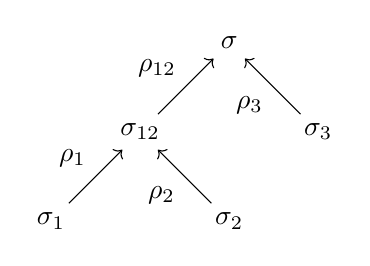
\begin{tikzpicture}
%\node(1) {$\sigma$};
%\node(2) [below right of=1] {$\sigma_{n}$};
%\node(3) [below left of=1] {$\sigma_{1\ldots n-1}$};
%\node(4) [below right of=3] {$\sigma_{n-1}$};
\node(5) {$\sigma$};
\node(6) [below right of=5] {$\sigma_{3}$};
\node(7) [below left of=5] {$\sigma_{12}$};
\node(8) [below right of=7] {$\sigma_2$};
\node(9) [below left of =7] {$\sigma_1$};
%\draw[loosely dotted] (6) to node {} (4);
%\draw[loosely dotted] (5) to node {} (3);
\draw[->] (9) to node {$\rho_1$} (7);
\draw[->] (7) to node {$\rho_{12}$} (5);
\draw[->] (6) to node {$\rho_{3}$} (5);
\draw[->] (8) to node {$\rho_2$} (7);
%\draw[->] (4) to node {$\rho_{n-1}$} (3);
%\draw[->] (3) to node {$\rho_{1\ldots n-1}$} (1);
%\draw[->] (2) to node {$\rho_{n}$} (1);
%\draw[->] (8) to [out=0, in=0, looseness=3] node [swap] {$i_2$} (1);
%\draw[->] (2) to [out=0, in=0, looseness=2] node  {$i_n$} (1);
%\draw[->] (4) to [out=0, in=0, looseness=3] node [swap] {$i_{n-1}$} (1);
%\draw[->] (6) to [out=0, in=0, looseness=3] node [swap] {$i_{n-1}$} (1);
\end{tikzpicture}
\]
The symbols $i_1$, $i_2$, and $i_3$ are function symbols with arity $\sigma_1\rightarrow \sigma$, $\sigma_2\rightarrow\sigma$, and $\sigma_3\rightarrow\sigma$, respectively.

We now turn to the proof.

\begin{proof}[Proof of Theorem \ref{mange}]
The following figure illustrates how our proof will be organized.
\begin{center}
\includegraphics{quineconjecture3revised.pdf}
\end{center}
Steps 1--3 define the theories $\widehat{T}_1,\ldots, \widehat{T}_{4}$, steps 4--6 define $T_1,\ldots, T_{4}$, and step 7 shows that $T_{4}$ and $\widehat{T}_{4}$ are logically equivalent.

\textbf{Step 1.} We begin by defining the theory $\widehat{T}_1$. For each sort $\sigma_j\in\Sigma$ we consider the following sentence.
\begin{align*}
\begin{aligned}
&\forall_\sigma y \left(q_{\sigma_j}(y)\leftrightarrow \exists_{\sigma_j} x(i_j(x)=y)\right) \\ &\qquad\land \forall_{\sigma_j} x_1\forall_{\sigma_j} x_2 (i_j(x_1)=i_j(x_2)\rightarrow x_1=x_2)
\end{aligned}
\tag{$\theta_{\sigma_j}$}
\end{align*}
The sentence $\theta_{\sigma_j}$ defines the symbols $\sigma_j$ and
$i_j$ as the subsort of ``things that are $q_{\sigma_j}$.'' The
auxiliary axioms $\phi_{\sigma_j}$ of $\widehat{T}$ guarantee that the
admissibility conditions for these definitions are satisfied. The
theory
$\widehat{T}_1=\widehat{T}\cup\{\theta_{\sigma_1},
\theta_{\sigma_2},\theta_{\sigma_3}\}$ is therefore a Morita extension
of $\widehat{T}$ to the signature
$\widehat{\Sigma}\cup\{\sigma_1,\sigma_2,\sigma_3, i_1,i_2,i_3\}$.

%We now show how the theory $\widehat{T}_1$ defines the new sorts $\sigma_{12}, \ldots, \sigma_{12,\ldots, n-1}$ and the function symbols $\rho_1, \rho_2, \ldots, \rho_{12\ldots n-1}, \rho_n$. 
\textbf{Step 2.} We now define the theories $\widehat{T}_2$ and $\widehat{T}_3$. Let $\theta_{\sigma_{12}}$ be a sentence that defines the symbols $\sigma_{12}, \rho_1, \rho_2$ as a coproduct sort. The theory $\widehat{T}_2=\widehat{T}_1\cup\{\theta_{\sigma_{12}}\}$ is clearly a Morita extension of $\widehat{T}_1$. 
%Likewise, the theory $\widehat{T}_1^1$ uses a sentence $\theta_{\sigma_{123}}$ to define the symbols $\sigma_{123}, \rho_{12}, \rho_3$ as a coproduct sort, resulting in another Morita extension $\widehat{T}_1^2=\widehat{T}\cup\{\theta_{\sigma_{12}}, \theta_{\sigma_{123}}\}$. 
%We repeat this process, at each step using the sentence $\theta_{\sigma_{1\ldots k}}$ to define the symbols $\sigma_{1\ldots k}$, $\rho_{1\ldots k-1}$, $\rho_k$ as coproduct sort, until we arrive at the theory 
%$$
%\widehat{T}_{n-1}=\widehat{T}_1\cup\{\theta_{\sigma_{12}}, \ldots, \theta_{\sigma_{1\ldots n-1}}\}
%$$
%in the signature $\widehat{\Sigma}\cup\{\sigma_1,\ldots, \sigma_n, i_1,\ldots, i_n\}\cup\{\sigma_{12},\ldots, \sigma_{12\ldots n-1}, \rho_1,\ldots, \rho_{n-1}\}$. One trivially sees that each $\widehat{T}_k$ that we have defined is a Morita extension of the theory $\widehat{T}_{k-1}$. 
%
We have yet to define the function symbols $\rho_{12}$ and $\rho_3$. The following two sentences define these symbols.
\begin{align*}
\tag{$\theta_{\rho_3}$}
&\forall_{\sigma_3} x \forall_\sigma y(\rho_3(x)=y\leftrightarrow i_3(x)=y)\\
%
&\forall_{\sigma_{12}} x \forall_\sigma y( \rho_{12}(x)=y\leftrightarrow \psi(x, y))
\tag{$\theta_{\rho_{12}}$}
\end{align*}
The sentence $\theta_{\rho_3}$ simply defines $\rho_3$ to be equal to the function $i_3$. For the sentence $\theta_{\rho_{12}}$, we define the formula $\psi(x,y)$ to be
%\begin{quote}
%Either (1) there is a $z$ such that $\rho_{n-1}(z)=z$ and $i_{n-1}(z)=y$ \textit{or} (2) there are $z_1$ and $z_2$ such that $\rho_{1\ldots n-2}(z_1)=x$, $\rho_{n-2}(z_2)=z_1$, and $i_{n-2}(z_2)=y$ \textit{or} \ldots \textit{or} ( 
%\end{quote}
\begin{align*}
&\exists_{\sigma_{1}} z_1 \big( \rho_{1}(z_1)=x\land i_{1}(z_1)=y\big)
\lor\exists_{\sigma_{2}} z_2\big( \rho_{2}(z_2)=x\land i_{2}(z_2)=y\big)
\end{align*}
We should take a moment here to understand the definition $\theta_{\rho_{12}}$. We want to define what the function $\rho_{12}$ does to an element $a$ of sort $\sigma_{12}$. Since the sort $\sigma_{12}$ is the coproduct of the sorts $\sigma_1$ and $\sigma_2$, the element $a$ must ``actually be'' of one of the sorts $\sigma_1$ or $\sigma_2$. (The disjuncts in the formula $\psi(x,y)$ correspond to these possibilities.) The definition $\theta_{\rho_{12}}$ stipulates that if $a$ is ``actually'' of sort $\sigma_j$, then the value of $\rho_{12}$ at $a$ is the same as the value of $i_j$ at $a$. One can verify that $\widehat{T}_{2}$ satisfies the admissibility conditions for $\theta_{\rho_3}$ and $\theta_{\rho_{12}}$, so the theory $\widehat{T}_3=\widehat{T}_{2}\cup\{\theta_{\rho_3}, \theta_{\rho_{12}}\}$ is a Morita extension of $\widehat{T}_{2}$ to the signature
$$
\widehat{\Sigma}\cup\{\sigma_1,\sigma_2, \sigma_3, \sigma_{12}, i_1,i_2, i_3, \rho_1, \rho_2,\rho_3, \rho_{12}\}
$$

\textbf{Step 3.} We now describe the $\Sigma^+$-theory $\widehat{T}_{4}$. This theory defines the predicates in the signature $\Sigma$. Let $p\in\Sigma$ be a predicate symbol of arity $\sigma_{j_1}\times\ldots\times\sigma_{j_m}$. We consider the following sentence.
\begin{align*}
\tag{$\theta_{p}$}
\forall_{\sigma_{j_1}} x_1\ldots \forall_{\sigma_{j_m}} x_m\left(p(x_1,\ldots, x_m)\leftrightarrow q_{p}(i_{j_1}(x_1),\ldots, i_{j_m}(x_m))\right)
\end{align*}
The theory $\widehat{T}_{4}=\widehat{T}_3\cup\{\theta_{p}:p\in\Sigma\}$ is therefore a Morita extension of $\widehat{T}_3$ to the signature $\Sigma^+$.

\textbf{Step 4.} We turn to the left-hand side of our organizational figure and define the theories $T_1$ and $T_{2}$. We proceed in an analogous manner to the first part of Step 2. The theory $T_1=T\cup\{\theta_{\sigma_{12}}\}$ is a Morita extension of $T$ to the signature $\Sigma\cup\{\sigma_{12}, \rho_1,\rho_2\}$. Now let $\theta_\sigma$ be the sentence that defines the symbols $\sigma, \rho_{12}, \rho_3$ as a coproduct sort. The theory $T_{2}=T_{1}\cup\{\theta_{\sigma}\}$ is a Morita extension of $T_{1}$ to the signature $\Sigma\cup\{\sigma_{12}, \sigma, \rho_1, \rho_2, \rho_3, \rho_{12}\}$.

\textbf{Step 5.} This step defines the function symbols $i_1$, $i_2$, and $i_3$. We consider the following sentences.
\begin{align*}
\tag{$\theta_{i_3}$}
&\forall_{\sigma_3} x_3 \forall_{\sigma} y(i_3(x_3)=y\leftrightarrow \rho_3(x_3)=y)\\
\tag{$\theta_{i_{2}}$}
%
&\forall_{\sigma_{2}}x_{2} \forall_{\sigma} y\big(i_{2}(x_{2})=y\leftrightarrow\exists_{\sigma_{12}} z( \rho_{2}(x_{2})=z\land\rho_{12}(z)=y)\big)\\
%
&\forall_{\sigma_1}x_1\forall_{\sigma}y\big(i_1(x_1)=y\leftrightarrow\exists_{\sigma_{12}} z(\rho_1(x_1)=z\land\rho_{12}(z)=y)\big)
\tag{$\theta_{i_1}$}
\end{align*}
The sentence $\theta_{i_3}$ defines the function symbol $i_3$ to be equal to $\rho_3$. The sentence $\theta_{i_{2}}$ defines the function symbol $i_{2}$ to be equal to the composition ``$\rho_{12}\circ\rho_{2}$.'' Likewise, the sentence $\theta_{i_{1}}$ defines the function symbol $i_{1}$ to be ``$\rho_{12}\circ\rho_{1}$.'' The theory $T_3=T_{2}\cup\{\theta_{i_1},\theta_{i_2}, \theta_{i_3}\}$
is a Morita extension of $T_{2}$ to the signature $\Sigma\cup\{\sigma_{12}, \sigma, \rho_1, \rho_2, \rho_3, \rho_{12}, i_1, i_2, i_3\}$.

\textbf{Step 6.} We still need to define the predicate symbols in $\widehat{\Sigma}$. Let $\sigma_j\in\Sigma$ be a sort symbol and $p\in\Sigma$ a predicate symbol of arity $\sigma_{j_1}\times\ldots\times\sigma_{j_m}$. We consider the following sentences.
\begin{align*}
&\begin{aligned}
\forall_{\sigma} y(q_{\sigma_j}(y)\leftrightarrow\exists_{\sigma_j} x(i_j(x)=y))
\end{aligned}
\tag{$\theta_{q_{\sigma_j}}$}\\
%
&\begin{aligned}
\forall_\sigma y_1\ldots\forall_\sigma y_m\big(q_{p}(y_1,\ldots, y_m)\leftrightarrow&\exists_{\sigma_{j_1}} x_1\ldots\exists_{\sigma_{j_m}} x_m(i_{j_1}(x_1)=y_1\land\ldots\\&\land i_{j_m}(x_m)=y_m\land p(x_1,\ldots, x_m))\big)
\end{aligned}
\tag{$\theta_{q_{p}}$}
\end{align*}
These sentences define the predicates $q_{\sigma_j}\in\widehat{\Sigma}$ and $q_p\in\widehat{\Sigma}$. One can verify that $T_3$ satisfies the admissibility conditions for the definitions $\theta_{q_{\sigma_j}}$. And therefore the theory $T_{4}=T_3\cup\{\theta_{q_{\sigma_1}}, \theta_{q_{\sigma_2}}, \theta_{q_{\sigma_3}}\}\cup\{\theta_{q_{p}}: p\in\Sigma\}$ is a Morita extension of $T_3$ to the signature $\Sigma^+$.

\textbf{Step 7.} It only remains to show that the $\Sigma^+$-theories
$T_{4}$ and $\widehat{T}_{4}$ are logically equivalent. One can verify
by induction on the complexity of $\psi$ that
\begin{equation}
  T_{4}\vdash\psi\leftrightarrow\widehat{\psi}\quad \text{and} \quad \widehat{T}_{4}\vdash\psi\leftrightarrow\widehat{\psi}.
\label{step7}
\end{equation}
for every $\Sigma$-sentence $\psi$. One then uses \eqref{step7} to
show that $T_{4}$ and $\widehat{T}_{4}$ are logically equivalent. The
argument involves a number of cases, but since each case is
straightforward we leave them to the reader to verify. The theories
$T_{4}$ and $\widehat{T}_{4}$ are logically equivalent, which implies
that $T$ and $\widehat{T}$ are Morita equivalent.
\end{proof}

Theorem \ref{mange} shows that Quine was right to say that every
many-sorted theory is equivalent to a single-sorted theory.  But what
is the philosophical significance of this result?  There is no doubt
about what Quine thought about its significance.  He claimed that
many-sorted logic was at best inessential, and at worst, a misleading
guide to the structure of knowledge and/or reality.  Whether he was
right or wrong, Quine has been almost single-handedly responsible for
the fact that many-sorted logic has not figured in the standard
curriculum for analytic philosophy students.  Indeed, far more
analytic philosophers are familiar with modal logic than are with
many-sorted logic (based on our anecdotal evidence from teaching,
reading journals, and talking with other philosophers).  We hope that
our efforts in this book go some way to fixing this problematic
situation.


\section{Translation generalized} \label{trans-g}

In the previous chapters, we've talked about various notions of a
``translation'' between theories.  Of course, we did not find the
definition of translation written on tablets of stone; nor did we have
a Platonic vision of the one true form of a translation.  No, we found
Quine's definition in the literature, and it works quite well for some
purposes, but it's also quite restrictive.  In particular, Quine's
notions of reconstrual and translation are not general enough to
capture some well-known cases of translations between the theories of
pure mathematics.

\begin{enumerate}
\item In the 19th century, the German mathematician Leopold Kronecker
  is reported to have said, ``God made the integers, all else is the
  work of man.''  In more prosaic terms, talk about higher number
  systems --- such as rational, real, and complex numbers --- can be
  {\it reduced} to talk about integers.  However, to effect such a
  reduction, one must treat each rational number as a pair of integers
  --- or, more accurately, as an equivalence class of pairs of
  integers.  Similarly, to reduce the complex numbers to the real
  numbers, one must treat a complex number as a pair of real numbers,
  viz.\ the real and imaginary parts of the complex number.
\item Now for a more controversial example, which we will take up at
  greater length in Section \ref{go-geometry}.  There are different
  ways that one can write down axioms for Euclidean geometry.  In one
  axiomatization, the basic objects are points; and in another
  axiomatization, the basic objects are lines.  Is there a sense in
  which these two axiomatized theories could both be Euclidean
  geometry, in particular, that they could be equivalent?  The answer
  is Yes, but only if one allows translations that take a single
  variable of the first theory to a pair of variables of the second
  theory.  In particular, a line needs to be treated as an equivalence
  class of pairs of points; and a point needs to be treated as a pair
  of intersecting lines.
\end{enumerate}

In the previous chapter, we required that a formula $p(x)$ of $\Sigma$
be translated to a formula $\vp (x)$ of $\Sigma '$.  There's one
particular part of this recipe that seems questionable: why would the
same variable $x$ occur in both formulas?  In general, why suppose
that two signatures $\Sigma$ and $\Sigma '$ should share the same
variables in common?  It's not like variables have some
``trans-theoretical'' meaning that must be preserved by any reasonable
translation.

But how then can variables be reconstrued in moving from one theory to
another?  One natural proposal would be to include in a reconstrual a
mapping from variables of $\Sigma$ to variables of $\Sigma '$, i.e.\ a
function that assigns a variable of $\Sigma '$ to each variable of
$\Sigma$.  Even so, it's a non-trivial question whether there is an
in-principle reason that a single variable in $\Sigma$ must be
reconstrued as a single variable in $\Sigma '$.  Perhaps one theorist
uses several variables to do the work that the other theorist manages
to do with a single variable.  Such cases are not hard to find in the
sciences --- for example, when the objects of one mathematical theory
are reconstrued as ``logical constructions'' of objects in another
mathematical theory.

Let's proceed then under the assumption that a single variable in one
language could be reconstrued in terms of multiple variables in
another language.  Thus, a reconstrual, in the formal sense, should
include a function that matches variables of the signature $\Sigma$ to
$n$-tuples of variables of the signature $\Sigma'$.

Consider again the case of reconstruing rational numbers (i.e.\
fractions) as pairs of integers.  Of course, not {\it every} pair of
integers gives a well-defined fraction.  For example, there is no
fraction of the form $\frac{1}{0}$.  In that case, the ``integer
theorist'' doesn't think of the domain of fractions as consisting of
all pairs of integers; rather, she thinks of that domain as consisting
of pairs of integers where the second entry is non-zero.  To capture
this nuance --- the restriction of the domain of quantification --- we
stipulate that a reconstrual $F$ includes a formula $D$ of the target
language $\Sigma '$.  In the running example, the formula $D$ could be
given by
\[ D(x,y) \: \equiv \: (x=x)\wedge (y\neq 0) .\] The integer theorist
can then use the formula $D$ to restrict her quantifiers to the domain
of well-defined fractions.

Finally, and most controversially, let's consider how we might
reconstrue the equality relation $=$ of the domain theory $T$ as a
relation of the target theory $T'$.  (Our choice here will prove to be
controversial when we show that it yields a positive verdict in favor
of quantifier variance.  See Example \ref{ex:nihil}.)  Recall that the
single variables $x$ and $y$ will typically be reconstrued as
$n$-tuples of variables $\vec{x}$ and $\vec{y}$.  In that case, how
should we reconstrue the formula $x=y$?  One might naturally propose
that $x=y$ be reconstrued as the formula
\begin{equation} (x_1=y_1)\wedge (x_2=y_2)\wedge \cdots \wedge
  (x_n=y_n) .\label{simple} \end{equation} But here we need to think a
bit harder about how and why variables of $\Sigma$ are encoded as
variables of $\Sigma '$.  For this, let's consider again the example
of rational numbers being reduced to integers:

Consider a formula $x=y$ in the theory of rational numbers.  To the
``integer theorist,'' the variables $x$ and $y$ really represent
complex entities, namely fractions.  What's more, to say that two
fractions $\frac{x_1}{x_2}$ and $\frac{y_1}{y_2}$ are equal does not
mean that $x_1=y_1$ and $x_2=y_2$.  Rather,
$\frac{x_1}{x_2}=\frac{y_1}{y_2}$ means that
$x_1\times y_2=y_1\times x_2$.  In other words, the formula $x=y$ of
the language of the rational numbers is reconstrued as the formula
\begin{equation} x_1\times y_2=y_1\times x_2
  ,\label{foo} \end{equation} in the language of the integers, where
$\times$ is the multiplication operation.

This example suggests that we might not always want the formula $x=y$
to be reconstrued as Eqn.\ \ref{simple}.  Instead, we might prefer to
reconstrue $x=y$ as some other $\Sigma '$ formula
$E(x_1,\dots ,x_n;y_1,\dots ,y_n)$.  Of course, not everything goes:
$E$ will need to perform the same functions in the theory $T'$ that
the formula $x=y$ performs in the theory $T$.  In particular, we will
require that $E$ be an equivalence relation relative to the theory
$T'$.

We're now ready to consider ways in which the elements of one
signature $\Sigma$ can be reconstrued as syntactic structures built
from a second signature $\Sigma '$.  (We include here the case where
$\Sigma '=\Sigma$.  In that case, we will be considering substitutions
and permutations of notation.)  The case of relation symbols is
relatively easy: an $m$-ary relation symbol $r$ of $\Sigma$ should
correspond to a formula $F(r)$ of $\Sigma '$ with $mn$ free variables.
To be even more precise, it's the relation symbol $r$ and an $n$-tuple
of variables $x_1,\dots ,x_n$ that corresponds to some particular
formula $F(r)$ of $\Sigma '$, and we require that
$FV(F(r))=\{ \vec{x}_1,\dots ,\vec{x}_n \}$.

We will need to proceed with more caution for the function symbols in
the signature $\Sigma$.  The question at issue is: which syntactic
structures over $\Sigma '$ are the proper targets for a reconstrual of
the function symbols in $\Sigma$?  To say that the target must be
another function symbol is too restrictive.  Indeed, there's a
well-known ``theorem'' which says that every first-order theory is
equivalent to a theory that uses only relation symbols.  (The reason
that ``theorem'' is placed in quotes here is because the result cannot
be proven with mathematical rigor until the word ``equivalent'' is
defined with mathematical rigor.)  The trick to proving that theorem
is to reconstrue each function symbol $f$ as a relation
\[ p_f(x_1,\dots ,x_m,y) \: \equiv \: (f(x_1,\dots ,x_m) = y) ,\] and
then to add axioms saying that $p_f$ relates each $m$-tuple
$x_1,\dots ,x_m$ to a unique output $y$.  If we are to be able to
validate such a result (which is intuitively correct), then we ought
to permit function symbols of $\Sigma$ to be reconstrued as formulas
of $\Sigma '$.  We will deal with this issue by analogy with the way
we dealt with relation symbols above: a function symbol $f$ of
$\Sigma$ and $m+1$ variables $x_1,\dots ,x_n,y$ of $\Sigma$ ought to
correspond to a formula $(Ff)(\vec{x}_1,\dots ,\vec{x}_n,\vec{y})$ of
$\Sigma '$.


  %% TO DO: straighten out notation for collection of sorts

  In order to define a more general notion of a translation, the key
  is to allow a single sort $\sigma$ of $\Sigma$ to be mapped to a
  sequence of sorts of $\Sigma '$, including the case of repetitions
  of a single sort.  The idea, in short, is to encode a single
  variable (or quantifier) in $\Sigma$ by means of several variables
  (or quantifiers) in $\Sigma '$.  In order to make this idea more
  clear, it will help to give a precise definition of the monoid of
  finite sequences from a set $S$.

  \begin{defn} For a set $S$, we let $S^*$ denote the \emph{free
      monoid} on $S$, which is uniquely defined by the following
    universal property: there is a function $\eta _S:S\to S^*$, and
    for any monoid $A$, and function $f:S\to A$, there is a unique
    monoid morphism $f^*:S^*\to A$ such that $f^*\circ\eta _S=f$.
    Concretely speaking, $S^*$ can be constructed as the set
  \[ S \amalg (S\times S)\amalg (S\times S\times S) \amalg \cdots ,\]
  where $\eta _S:S\to S^*$ is the first coprojection.  In this case,
  given $f:S\to A$, $f^*:S^*\to A$ is the function
  \[ f^*(s_1,\dots ,s_n) \: = \: f(s_1)\circ \cdots\circ f(s_n) ,\]
  where $\circ$ is the monoid operation on $A$.  \end{defn}

\begin{defn} \label{gro} Let $\Sigma$ and $\Sigma '$ be many-sorted
  signatures with sets of sorts $S$ and $S'$ respectively.  A
  generalized \emph{reconstrual} $F:\Sigma \to \Sigma '$ consists of:
  \begin{enumerate}
  \item A function $F:S\to (S')^*$.  That is, $F$ maps the sorts of
    $\Sigma$ to non-empty sequences of sorts of $S'$.  For each
    $\sigma\in S$, let $d(\sigma )$ be the length of the sequence
    $F(\sigma )$.  We call $d:S\to\7N$ the \emph{dimension function}
    of $F$.
  \item A corresponding function
    $x\mapsto \vec{x}=x_1,\dots ,x_{d(\sigma )}$ from
    $\Sigma$-variables to sequences of $\Sigma '$-variables, such that
    $x_i:F(\sigma )_i$.  We require that if $x\not\equiv y$, then the
    sequences $\vec{x}$ and $\vec{y}$ have no overlap.
  \item A function $D$ from $\Sigma$-variables to $\Sigma '$-formulas.
    We call $D_x$ a \emph{domain formula}.  We require the map
    $x\mapsto D_x$ to be natural in the following sense: if $y$ is of
    the same sort as $x$, then $D_y=D_x[\vec{y}/\vec{x}]$.
  \item A function $F$ that takes a relation symbol $p$ of $\Sigma$,
    and a suitable context $x_1,\dots ,x_n$ of variables from
    $\Sigma$, and yields a formula $(Fp)(\vec{x}_1,\dots ,\vec{x}_n)$
    of $\Sigma '$.  We again require this map to be natural in the
    sense that
    \[ (Fp)(\vec{y}_1,\dots ,\vec{y}_n) \: = \: (Fp)(\vec{x}_1,\dots
      ,\vec{x}_n)[\vec{y}_1,\dots ,\vec{y}_n/\vec{x}_1,\dots
      ,\vec{x}_n] .\] \end{enumerate}
\end{defn}


%    \item For each sort symbol $\sigma\in S$, a natural map $E^\sigma$
%     from pairs of variables of sort $\sigma$ to a formula with pairs
%     of variables of sort $F(\sigma )$.  Thus, $E^\sigma_{x,y}$ is a
%     $\Sigma '$-formula with free variables
%     $\vec{x}=x_1,\dots ,x_{d(\sigma )}$ and
%     $\vec{y}=y_1,\dots ,y_{d(\sigma )}$, where $d(\sigma )$ is the
%     length of the sequence $F(\sigma )$.  To say that $E_\sigma$ is
%     natural means that
%     $E_\sigma (v,w)=E_\sigma (x,y)[\vec{v},\vec{w}/\vec{x},\vec{y}]$,
%     or in diagrammatic form:
%     \[ \begin{tikzcd} v,w\arrow{r}{[x,y/v,w]} \arrow{d} & x,y \arrow{d} \\
%         E_\sigma (v,w) \arrow{r}{[\vec{x},\vec{y}/\vec{v},\vec{w}]} &
%         E_\sigma (x,y) \end{tikzcd} \] We write $D_\sigma (x)$ for
%     $E _\sigma (x,x)$, and call $D_\sigma (x)$ a \emph{domain
%       formula}.  When no confusion can result, we drop the $\sigma$
%     from $E_\sigma$ and $D_\sigma$.
%   \item We require that each $E(x,y)$ is a non-empty, partial
%     equivalence relation in the sense that
%     \[ \vdash \exists \vec{x} E(x,x) \qquad E(x,y)\vdash E(y,x) \qquad
%       E(x,y)\wedge E(y,z)\vdash E(x,z) \] Thus, $E(x,y)$ is a full
%     equivalence relation on domain $D(x)$.
   
% \item For each function symbol $f\in\Sigma$, we define $Ff$ as a
%   natural map from contexts for $f$ to $\Sigma '$-formulas.  More
%   precisely: if $x_1,\dots ,x_n$ is an appropriate context for $f$,
%   and $y$ is of the output sort for $f$, then $F(f)(x_1,\dots ,x_n,y)$
%   is a $\Sigma _2$-formula with free variables
%   $\vec{x}_1,\dots ,\vec{x}_n,\vec{y}$ of the appropriate sorts.  We
%   require that $Ff$ is natural under substitution of variables, is
%   compatible with the equivalence relation $E(\vec{x},\vec{y})$, and
%   is a functional relation from $D(\vec{x})$ to $D(\vec{y})$, relative
%   to $E(\vec{x},\vec{y})$:
%   \[ (Ff)(x,y)\wedge (Ff)(x,z) \:\vdash \:E(\vec{y},\vec{z}) \]
%   \[ D(\vec{x}) \:\vdash \: \exists\vec{y}(Ff)(x,y) \]
% \end{enumerate}
% \end{defn}

% This definition may seem too complicated for any practical use.
% However, it's actually fairly easy to define legitimate reconstruals
% without thinking too hard about all of these conditions.  In short, if
% $\sigma$ goes to a sequence $\sigma _1,\dots ,\sigma _n$, then we need
% to map equality on $\sigma$ to some equivalence relation $E$ on
% $\sigma _1,\dots ,\sigma _n$.  Then for each relation symbol $p$ of
% $\Sigma$, we define $(Fp)(x_1,\dots ,x_n)$ to be a $\Sigma '$-formula
% $\phi (\vec{x}_1,\dots ,\vec{x}_n)$, with the implicit understanding
% then that $(Fp)(y_1,\dots ,y_n)$ is the formula
% $\phi (\vec{y}_1,\dots ,\vec{y}_n)$ that results from uniform
% substitution.  Function symbols are a bit more tricky, since we map
% them not to function symbols, but to relation symbols.  However, given
% a function symbol $f$ of $\Sigma$, we map $f(x_1,\dots ,x_n)=y$ to a
% relation symbol $\phi (\vec{x}_1,\dots ,\vec{x}_n,\vec{y})$, again
% with the understanding that substitutions on the domain formula
% correspond to appropriate substitutions on the codomain formula.

A reconstrual $F$ naturally extends to a map from $\Sigma$-formulas to
$\Sigma '$-formulas.  We define this extension, also called $F$, so
that for any $\Sigma$-formula $\phi$, with $x$ free in $\phi$, the
following two constraints are satisfied:
\[ F(\phi )\:\vdash \: D(\vec{x}) ,\qquad \qquad F(\phi [y/x]) \: = \:
  F(\phi )[\vec{y}/\vec{x}] , \] The first restriction is not
technically necessary --- it is simply a convenient way to ignore
whatever the formula $F(\phi )$ says about things outside of the
domain $D(\vec{x})$.  (This apparently minor issue plays a significant
role in Quine's argument for the dispensability of many-sorted logic.
See \ref{qboom}.)  Accordingly, for a relation symbol $p$ of $\Sigma$,
we first redefine $(Fp)(\vec{x}_1,\dots ,\vec{x}_n)$ by conjoining
with $D(\vec{x}_1)\wedge\cdots\wedge D(\vec{x}_n)$.  (We could have
also have included this condition in the very definition of a
reconstrual.)  The extension of $F$ proceeds as
follows: \begin{itemize}
\item Let $F(\phi\wedge \psi )=F(\phi )\wedge F(\psi )$, and let
  $F(\phi\vee\psi )=F(\phi )\vee F(\psi )$. 
\item Let
  $F(\neg \phi ) =\neg F(\phi )\wedge D(\vec{x}_1)\wedge\cdots\wedge
  D(\vec{x}_n)$, where $x_1,\dots ,x_n$ are all the free variables
  that occur in $\phi$.
\item Let $F(\phi\to\psi )=F(\neg\phi )\vee F(\psi )$.
\item Let
  $F(\exists x\phi )=\exists \vec{x}(D(\vec{x})\wedge F(\phi ))$.
\item Let $F(\forall x\phi )=\forall \vec{x}(D(\vec{x})\to F(\phi ))$.
\end{itemize}
  
\begin{defn} Let $F:\Sigma \to\Sigma '$ be a reconstrual.  We say that
  $F$ is a \emph{translation} of $T$ into $T'$ just in case: for every
  $\Sigma$-sentence $\phi$: if $T\vdash\phi$ then $T'\vdash F(\phi )$.
  In this case, we write $F:T\to T'$.  In the case that $\Sigma$ has a
  single sort $\sigma$, we say that $F$ is a $d(\sigma )$-dimensional
  translation.  \end{defn}

The definition of a translation allows us to handle the case where the
domain signature $\Sigma$ has equality relations and function symbols.
In particular, for each theory $T$ in $\Sigma$, we explicitly include
the following axioms:
\begin{itemize}
\item The equality introduction axioms: $\vdash x=_\sigma x$.
\item The equality elimination axioms:
  $\phi (x),(x=_\sigma y)\vdash \phi (y)$, for each atomic or negated
  atomic formula $\phi$ of $\Sigma$.
\end{itemize}
As usual, these axioms together entail that $=_\sigma$ is an
equivalence relation.  Thus, if $F:T\to T'$ is a translation, then
$F(=_\sigma )(\vec{x},\vec{y})$ is an equivalence relation on domain
$D(\vec{x})$.  We abbreviate this relation by
$E_\sigma (\vec{x},\vec{y})$, or when no confusion can result, simply
as $E(\vec{x},\vec{y})$.  In this case, for each relation symbol $p$
of $\Sigma$, 
\[ T',(Fp)(\vec{x}), E(\vec{x},\vec{y})\:\vdash \: (Fp)(\vec{y}) .\]
Roughly speaking, the predicate $Fp$ has to be compatible with the
equivalence relation $E$: it holds of something iff it holds of
everything $E$-equivalent to that thing.  Equivalently, the extension
of $Fp$ is a union of $E$-equivalence classes.

Now suppose that $\Sigma$ contains a constant symbol $c$.  Then,
choosing a variable $x$ of the same sort, $c=x$ is a unary formula,
and $F(c=x)$ is a formula $\phi (\vec{x})$.  The theory $T$ entails
that the formula $c=x$ is uniquely satisfied.  Hence, if $F:T\to T'$
is a translation, then $T'$ entails that $\phi (\vec{x})$ is uniquely
satisfied --- relative to the equivalence relation $E$.  In short $T'$
implies both $\exists \vec{x}(D_x\wedge \phi (\vec{x}))$ and
$\phi (\vec{x})\wedge \phi (\vec{y})\to E(\vec{x},\vec{y})$.
Intuitively speaking, this means that the extension of
$\phi (\vec{x})$ is a single $E$-equivalence class.

Similar reasoning applies to the case of any function symbol $f$ of
$\Sigma$.  The $\Sigma$-formula $f(x_1,\dots ,x_n)=y$ is reconstrued
as some $\Sigma '$-formula
$\phi (\vec{x}_1,\dots ,\vec{x}_n,\vec{y})$.  If $F:T\to T'$ is a
translation, then $T'$ entails that $\phi$ is a functional relation
relative to $E$-equivalence.  What this means intuitively is that
$\phi$ is a function from $E$-equivalence classes to $E$-equivalence
classes.

%%% Examples

\begin{example}[Quantifier variance] \label{go-qv} We now undertake an
  extended discussion of an example that is near and dear to
  metaphysicians: the debate between mereological universalism and
  nihilism.  To keep the technicalities to a bare minimum, we will
  consider a dispute over whether the composite of two things exists.
  Suppose that the parties to the dispute are are named Niels the
  Nihilist and Mette the Mereological Universalist.  Niels says that
  there are exactly two things, whereas Mette says that there are
  exactly three things, one of which is composed of the other two.

  Now, we press Niels and Mette to regiment their theories, and here's
  what they come up with.  Niels has a signature $\Sigma$, which is
  empty, very much in line with his predilection for desert
  landscapes.  Niels' theory has a single axiom, ``there are exactly
  two things.''  Mette has a signature $\Sigma '$ with a binary
  relation symbol $p$ that she'll use to express the parthood
  relation.  Mette's theory $T'$ says that $p$ is a strict partial
  order, that there are exactly two atoms, and exactly one thing above
  those two atoms.  Note that Mette can define an open formula in
  $\Sigma '$
  \[ a(x) \: \equiv \: \neg \exists y\, p(y,x) ,\] which intuitively
  expresses the claim that $x$ is an atom.

  At the turn of the 21st century, metaphysicians were engaged in a
  fierce debate about whether Niels or Mette has a better theory.
  Then some other philosophers, such as Eli Hirsch, said, ``stop
  arguing --- it's merely a verbal dispute, like an argument about
  whether there are six roses or half a dozen roses''
  \citep[see][]{chalmers,hirschbog}.  These other philosophers espouse
  a position known as \emph{quantifier variance}.  One clear
  explication of quantifier variance would be to say that Niels and
  Mette's theories are \emph{equivalent}.  So are they equivalent or
  not?  The answer to this question depends (unsurprisingly) on the
  standard of equivalence that we adopt.  For example, it is easy to
  see that Niels and Mette's theories are not strictly
  intertranslatable in the sense of Defn \ref{def:itrans}.  However,
  we will now see that Niels and Mette's theories are
  intertranslatable in the weaker sense described in Defn
  \ref{def:weak}.

  It seems clear that Mette can make sense of Niels' theory --- in
  particular, that she can identify Niels' quantifier as a restriction
  of her own.  The idea that Mette can ``make sense of Niels' theory''
  can be cashed out formally as saying that Niels' theory can be
  translated into Mette's theory.  Intuitively speaking, for any
  sentence $\phi$ asserted by Niels, there is a corresponding sentence
  $\phi ^*$ asserted by Mette.  For example, when Niels says
  \begin{quote} There are exactly two things,
  \end{quote}
  Mette can charitably interpret him as saying, 
  \begin{quote}
    There are exactly two atoms. \end{quote}

  Now we show that there is indeed a translation $F:T\to T'$, where
  $T$ is Niels' theory, and $T'$ is Mette's theory.  Here Niels and
  Mette's theories are single-sorted, and we define $F$ to be a
  one-dimensional reconstrual.  We define the domain formula as
  $D_F(x)=a(x)$, and we translate Niels' equality relation as Mette's
  equality relation restricted to $D_F$.

  Let's just check that $F$ is indeed a translation.  While a general
  argument is not difficult, let's focus on Niels' controversial
  claim $\phi$: that there are {\it at most two} objects in the domain: 
  \[ \phi \:\equiv \: \forall x\forall y\forall z((x=y)\vee (x=z)\vee
    (y=z)) .\] The reconstrual $F$ takes $x=y$ to the formula
  $a(x')\wedge a(y')\wedge (x'=y')$, and hence $F(\phi )$ is the
  uncontroversially true statement that there are at most two atoms.
  Of course, Mette agrees with that claim, and so $F:T\to T'$ is a
  translation of Niels' theory into Mette's.

  Indeed, $F$ is a particularly nice translation: it's conservative,
  in the sense that if $T'\vdash F(\phi )$ then $T\vdash \phi$.  Thus,
  not only does Mette affirm everything that Niels says about atoms,
  Niels also affirms everything that Mette says about atoms.  Thus,
  there is a precise sense in which Niels' theory is simply a
  ``sub-theory'' of Mette's theory.  They are in complete agreement
  relative to their shared language, and Mette simply has a larger
  vocabulary than Niels.

  The existence of the translation $F:T\to T'$ comes as no surprise.
  But what about the other way around?  Can Niels be as charitable to
  Mette as she has been to him?  Can he find a way to affirm {\it
    everything} that she says?  The answer to that question is far
  from clear.  For example, Mette says things like, ``$x$ is a
  composite of $y$ and $z$.''  How in the world could Niels make sense
  of that claim?  How in the world could Niels say, ``what Mette says
  here is perfectly correct, if only understood in the proper way''?
  Similarly, Mette says that ``there are more than two things.''  How
  in the world could Niels validate such a claim?

  We will now see that Niels can indeed charitably interpret, and
  endorse, all of Mette's assertions.  Indeed, Niels needs only think
  of Mette's notion of ``a thing'' as corresponding to what he means
  by ``a pair of things'' --- as long as two pairs are considered to
  be ``the same'' when they are permutations of each other.

  More precisely, consider a $2$-dimensional reconstrual
  $G:\Sigma '\to \Sigma$ which encodes a $\Sigma '$-variable $x$ as a
  pair $x_1,x_2$ of $\Sigma$-variables.  Define $D_G(x_1,x_2)$ to be
  the formula $(x_1=x_1)\wedge (x_2=x_2)$ that holds for all pairs
  $\langle x_1,x_2\rangle$.  Define $E_G(x_1,x_2,y_1,y_2)$ to be the
  relation that holds between $\langle x_1,x_2\rangle$ and
  $\langle y_1,y_2\rangle$ just in case one is a permutation of the
  other.  That is,
  \[ E_G(x_1,x_2,y_1,y_2) \: \equiv \: (x_1=y_1\wedge x_2=y_2)\vee
    (x_1=y_2\wedge x_2=y_1 ) .\] Clearly $T$ entails that $E_G$ is an
  equivalence relation.

  The signature $\Sigma '$ consists of a single binary relation symbol
  $p$.  Since $G$ is $2$-dimensional, $Gp$ must be defined to be a
  four-place relation in $\Sigma$.  Here is the intuitive idea behind
  our definition of $Gp$: we will simulate atoms of Mette's theory by
  means of diagonal pairs, i.e.\ pairs of the form
  $\langle x,x\rangle$.  We then say that $Gp$ holds precisely between
  pairs when the first is diagonal, the second is not, and the first
  has a term in common with the second.  More precisely,
  \[ (Gp)(x_1,x_2,y_1,y_2) \: \equiv \: (x_1=x_2)\wedge (y_1\neq y_2
    )\wedge (x_1=y_1\vee x_1=y_2) .\] Recall that $a(x)$ is the
  formula of $\Sigma '$ which says that $x$ is an atom.  We claim now
  that the translation $G(a(x))$ of $a(x)$ holds precisely for the
  pairs on the diagonal.  That is,
  \[ T\:\vdash \: G(a)(x_1,x_2)\leftrightarrow (x_1=x_2 ) .\] We argue
  by reductio ad absurdum.  (Here we use the notion of a model, which
  will first be introduced in the next chapter.  Hopefully the
  intuition here is clear.)  First, if
  \[ T\:\not\vdash \: G(a)(x_1,x_2)\rightarrow (x_1=x_2 ), \] then
  there is a model $M$ of $T$, and two distinct objects $c,d$ of $M$
  such that $M\models G(a)(c,d)$.  That means that
  \[ M\models \neg \exists y\exists z\, G(p)(y,z,c,d) .\] But clearly
  $M\models G(p)(c,c,c,d)$, a contradiction.  To prove the other
  direction it will suffice to show that for any model $M$ of $T$, and
  for any $c\in M$, we have $M\models G(a)(c,c)$.  Recalling that $T$
  only has one model, namely a model with two objects, the result
  easily follows.
  
  When Mette the Mereologist says that there are more than two things,
  Niels the Nihilist understands her as saying that there are more
  than two pairs of things.  Of course, Niels agrees with that claim.
  In fact, it's not hard to see that, under this interpretation, Niels
  affirms everything that Mette says. \end{example}

\begin{disc} We've shown that Niels' theory can be translated into
  Mette's, and vice versa.  Granting that this is a good notion of
  ``translation,'' does it follow that these two theories are
  equivalent?  In short, No.  Recall the simpler case of propositional
  theories.  For example, let $\Sigma = \{ p_0,p_1,\dots \}$, let $T$
  be the empty theory in $\Sigma$, and let $T'$ be the theory with
  axioms $p_0\vdash p_1,p_0\vdash p_2,\dots $.  Then there are
  translations $f:T\to T'$ and $g:T'\to T$, but $T$ and $T'$ are not
  equivalent theories.  In general, mutual translatability is not
  sufficient for equivalence.  Nonetheless, we will soon see (Example
  \ref{ex:nihil}) that there is a precise sense in which Niels and
  Mette's theories are indeed equivalent.  \hfill \qed
\end{disc}

We are now ready to prove a generalized version of the
\textbf{substitution theorem}.  In its simplest form, the substitution
theorem says a valid derivation $\vp _1,\dots ,\vp_n\vdash \psi$ is
preserved under uniform substitution of the non-logical symbols in
$\phi _1,\dots ,\phi _n$ and $\psi$.  For example, from a valid
derivation of $\exists x(p(x)\wedge q(x))\vdash \exists x p(x)$,
substitution of $\forall y(r(y,z)$ for $p(x)$ yields a valid
derivation of
\[ \exists z(\forall yr(y,z)\wedge q(z)) \: \vdash \: \exists z\forall
  yr(y,z) .\] However, we need to be careful in describing what counts
as a legitimate ``substitution instance'' of a formula.  Let's test
our intuitions against an example.

\begin{example} Let $\Sigma$ be a single-sorted signature with
  equality, but no other symbols.  Let $\Sigma '$ be a single-sorted
  signature with equality, and one other monadic predicate $D(x)$.  We
  define a 1-dimensional reconstrual $F:\Sigma\to\Sigma '$ by taking
  $D(x)$ to be the domain formula, and by taking $E(x,y)$ to be
  equality in $\Sigma '$.  We will see now that the substitution
  theorem does {\it not} hold in the form: if $\phi\vdash\psi$ then
  $F(\phi)\vdash F(\psi )$.

  In $\Sigma$ we have $x\neq y \vdash \exists z(x\neq z)$.  Since $F$
  translates equality in $\Sigma$ to equality in $\Sigma '$, we have
  $F(x\neq y)\equiv (x\neq y)$.  Furthermore, $F(\exists z(x\neq z))$
  is the relativized formula $\exists z(D(z)\wedge x\neq z)$.  But
  $x\neq y$ does not imply there there is a $z$ such that $D(z)$ and
  $x\neq z$.  For example, in the domain $\{ a,b\}$, if the extension
  of $D$ is $\{ a\}$, then $a\neq b$, but not
  $\exists z(D(z)\wedge a\neq z)$.  Thus, the substitution theorem
  does {\it not} hold in the form: if $\phi\vdash\psi$ then
  $F(\phi )\vdash F(\psi )$.  So what's the problem here?

  To speak figuratively, a reconstrual $F$ maps a variable $x$ of
  $\Sigma$ to variables $\vec{x}$ that are relativized to the domain
  $D(\vec{x})$.  However, the turnstyle $\vdash$ for $\Sigma '$ is not
  relativized in this fashion: a sequent $F(\phi )\vdash F(\psi )$
  corresponds to a tautology
  $\vdash \forall \vec{x}(F(\phi )\to F(\psi ))$.  It wouldn't make
  sense to expect this last statement to hold, since the intention is
  for the variables in $F(\phi )$ and $F(\psi )$ to range over
  $D(\vec{x})$.  Thus, the relevant question is whether
  $F(\phi )\vdash _{D(\vec{x})} F(\psi )$, where the latter is
  shorthand for
  \[ \vdash \forall \vec{x}(D(\vec{x})\to (F(\phi )\to F(\psi ))) .\]
  In the current example, then, the question is whether the following
  holds:
  \[ F(x\neq y), D(x),D(y) \:\vdash \: F(\exists y(x\neq y)) .\] And
  it obviously does.  This example shows us how to formulate a
  substitution theorem for generalized reconstruals such as $F$.
  \hfill \qed \end{example}

\begin{thm}[Substitution] Let $\Sigma$ be a signature without function
  symbols, and suppose suppose that $F$ is a reconstrual from $\Sigma$
  to $\Sigma '$.  Then for any formulas $\phi$ and $\psi$ with free
  variables $x_1,\dots ,x_n$, if $\vp\vdash\psi$ then
  $F(\phi )\vdash _{D(\vec{x}_1,\dots ,\vec{x}_n)}F(\psi )$.  In
  particular, if $\phi$ and $\psi$ are $\Sigma$-sentences then
  $F(\phi )\vdash F(\psi )$.
\end{thm}

\begin{proof} We will prove this result by induction on the
  construction of proofs.  For the base case, the rule of assumptions
  justifies not only $\vp\vdash\vp$, but also $F(\vp )\vdash F(\vp )$,
  and hence $D(\vec{x}),F(\phi )\vdash F(\phi )$. The inductive cases
  for the Boolean connectives involve no special complications, and so
  we leave them to the reader.

  Consider now the case of $\exists$-elim.  Suppose that
  $\exists y\vp \vdash \psi$ results from application of
  $\exists$-elim to $\vp\vdash\psi$, in which case $y$ is not free in
  $\psi$.  We rewrite $\vp$ and $\psi$ in the suggestive notation
  $\vp (x,y)$ and $\psi (x)$, indicating that $x$ may be free in both
  $\vp$ and $\psi$, and that $y\not\equiv x$.  (Note, however, that
  our argument doesn't depend on $\vp$ and $\psi$ sharing exactly one
  free variable in common.  We want to show that
  $F(\exists y\vp (x,y))\vdash _{D(\vec{x})}F(\psi (x))$, which
  expands to
  \begin{equation} D(\vec{x}),\exists \vec{y}(D(\vec{y})\wedge F(\vp
    (x,y))) \: \vdash \: F(\psi (x)) . \label{G2} \end{equation} The
  inductive hypothesis here says that
  \[ D(\vec{x}),D(\vec{y}),F(\vp (x,y)) \:\vdash \: F(\psi (x)) .\]
  Since $x$ and $y$ are distinct variables, the sequences $\vec{x}$
  and $\vec{y}$ have no overlap, and $\vec{y}$ does not occur free in
  $D(\vec{x})$.  Thus, $n$-applications of $\exists$-intro yield the
  sequent (\ref{G2}).

  Consider now the case of $\exists$-intro.  Suppose that
  $\vp\vdash \exists y\psi$ follows from $\vp\vdash\psi$ by an
  application of $\exists$-intro.  Again, we will rewrite the former
  sequent as
  \[ \vp (x,y)\: \vdash \: \exists y\psi (x,y) .\]
  We wish to show that
  \[ D(\vec{x}),D(\vec{y}),F(\vp (x,y)) \: \vdash \: \exists
    \vec{y}F(\psi (x,y)) .\] By the inductive hypothesis, we have
  \[ D(\vec{x}),D(\vec{y}),F(\vp(x,y))\: \vdash \: F(\psi (x,y)) .\]
  Thus, the result follows by repeated application of $\exists$-intro.
\end{proof}

The previous version of the substitution theorem applies only to the
case of signatures without function symbols.  Intuitively, however,
the formal validity of proofs should also be maintained through
uniform substitution of terms.

\begin{example} Suppose that $\vp (x)\vdash \psi (x)$, which is
  equivalent to $\vdash \forall x(\vp (x)\vdash \psi (x))$.  Now let
  $t(\vec{y})$ be a term with free variables
  $\vec{y}\equiv y_1,\dots ,y_n$, and suppose that each of these
  variables is free for $x$ in $\vp$ and $\psi$, but none of them are
  themselves free in either one of these formulas.  (In the simplest
  case, these variables simply do not occur in either one of the
  formulas.)  Then $\forall$-elim and intro yield
  $$ \vdash \forall \vec{y} (\vp (t(\vec{y}))\to \psi (t(\vec{y} )) ) ,$$
  which is equivalent to $\vp (t(\vec{y})\vdash \psi (t(\vec{y}))$.
  In other words, a valid proof remains valid if a variable $x$ is
  uniformly replaced by a term $t(\vec{y})$, so long as the relevant
  restrictions are respected. \hfill \qed
\end{example}


At this stage, we have a definition of a generalized translation; and
we've shown that it yields a generalized substitution theorem.  What
we would like to do now is to look at specific sorts of translations
--- and most particularly, at which translations should count as
giving an equivalence of theories.  It turns out, however, that giving
a good definition of equivalence is a bit complicated.  As many
examples will show, it won't suffice to say that a translation
$F:T\to T'$ is an equivalence just in case it has an inverse
$G:T'\to T$, and not even a quasi-inverse in the sense of
\ref{def:itrans}.  For a good definition of equivalence, we need a
notion of a ``homotopy'' between translations, and we need a notion of
the composition of translations.  We turn first to the second of
these.

\begin{defn}[Composition of reconstruals] Suppose that
  $F:\Sigma\to \Sigma _1$ and $G:\Sigma _1\to \Sigma _2$ are
  reconstruals.  Define a reconstrual $H:\Sigma \to\Sigma _2$ as
  follows:
  \begin{itemize}
  \item Since $G:S_1\to S_2^*$, there is a unique morphism
    $G^*:S_1^*\to S_2^*$ such that $G=G^*\circ \eta _{S_1}$.  In other
    words, $G^*$ acts on a sequence of $S_1$ sorts by applying $G$ to
    each element and then concatenating.  We then define
    $H=G^*\circ F:S\to S^*_2$.
  \item We use the same idea as above to associate each variable $x$
    of $\Sigma$ with a (double) sequence $X_1,\dots ,X_n$ of variables
    of $\Sigma _2$.  In short,
    \[ \begin{array}{l l l} H(x) & = & G^*(F(x))  \\
                                 & = & X_1,\dots
                                       ,X_n \\
                                 & = & (x_{11},\dots ,x_{1m_1}),\dots
                                       ,(x_{n1},\dots ,x_{nm_n})
                                       , \end{array} \] where
                                       $F(x)=x_1,\dots ,x_n$, and
                                       $G(x_i)=X_i=(x_{i1},\dots
                                       ,x_{im_i})$.
    
  \item Let $D_F(\vec{x})$ denote the domain formula of $F$
    corresponding to the $\Sigma$-variable $x$.  Let $D_G(X_i)$ denote
    the domain formula of $G$ corresponding to the
    $\Sigma _1$-variable $x_i$.  Then we define
    \[ D_H(X_1,\dots ,X_n) \: := \: G(D_F(\vec{x})) .\] Recall that
    any free variable in $G(D_F(\vec{x}))$ occurs in the
    double-sequence $X_1,\dots ,X_n$; and that $G(\phi )\vdash D_G(Y)$
    if $y$ is free in $\phi$.  Thus,
    $D_H(X_1,\dots ,X_n)\vdash D_G(X_i)$ for each $i=1,\dots ,n$.
  \item For a relation symbol $p$ of $\Sigma$, we define
    \[ (Hp)(X_1,\dots ,X_n) \: = \: G((Fp)(\vec{x}_1,\dots
      ,\vec{x}_n)) .\] 
   \end{itemize} \end{defn}
%    recalling that $L$ ambiguously denotes a reconstrual
%    $L:\Sigma _2\to\Sigma _3$, and a map from $\Sigma _2$-formulas to
%    $\Sigma _3$-formulas.  We need to check that
%     \[ L(K(p))\vdash _{\vec{x}:LK(\sigma )} \eta _\sigma ,\] where we
%     have assumed for notational simplicity that $p:\sigma$.  Since $K$
%     is a reconstrual, $K(p):K(\sigma )$, and since
%     $\langle L,\epsilon\rangle$ is a reconstrual,
%     \[ L(K(p))\vdash _{\vec{x}:LK(\sigma )} \epsilon _{K(\sigma )} .\]
%     Again, since $\langle K,\delta \rangle$ is a reconstrual,
%     \[ K(p)\vdash _{\vec{y}:K(\sigma )} \delta _\sigma ,\]
%     and so, by the substitution theorem,
%     \[ L(K(p))\vdash _{\vec{x}:LK(\sigma )} L(\delta _{\sigma }) .\]
%     (Here the admissibility conditions are automatically satisfied
%     since $L$ is a translation into $T_3$.)  Putting these two
%     together, we have
%     \[ L(K(p))\vdash _{\vec{x}:LK(\sigma )} \epsilon _{K(\sigma
%         )}\wedge L(\delta _{\sigma }) ,\]
%     as was to be shown.  \end{itemize}
% \end{defn}'

 \begin{prop} If $F$ and $G$ are translations, then $G\circ F$ is a
   translation. \end{prop}

 \begin{proof} This result follows trivially once we recognize that
   $G\circ F$ is a legitimate reconstrual.  \end{proof}


 For some philosophers, it may seem that we have already greatly
 overcomplicated matters by using category theory to frame our
 discussion of theories.  I'm sorry to say that matters are worse than
 that.  The collection of theories really has more interesting
 structure than a category has; in fact, it's most naturally thought
 of as a \emph{2-category}, where there are 0-cells (objects), 1-cells
 (arrows), and 2-cells (arrows between arrows).  In particular, our
 $2$-category of theories, $\mathbf{Th}$, has first-order theories as
 the 0-cells, and translations as the 1-cells.  We now define the
 2-cells, which we call \textbf{t-maps}.  

Let $F$ and $G$ be translations from $T$ to $T'$.  Since the
definition of a t-map is heavily syntactic, we begin with an intuitive
gloss in the special case where $\Sigma$ has a single sort $\sigma$.
In this case $F(\sigma )$ is a sequence $\sigma _1,\dots ,\sigma _m$
of $\Sigma '$-sorts, and $G(\sigma )$ is a sequence
$\sigma '_1,\dots ,\sigma '_n$ of $\Sigma '$-sorts.  Then a t-map
$\chi :F\Rightarrow G$ consists of a formula $\chi (\vec{x},\vec{y})$
that links $m$-tuples to $n$-tuples.  This formula
$\chi (\vec{x},\vec{y})$ should have the following features:
\begin{enumerate}
\item The theory $T'$ implies that $\chi (\vec{x},\vec{y})$ is a
  functional relation from $D_F$ to $D_G$, relative to the notion of
  equality given by the equivalence relations $E_F$ and $E_G$.
\item For each formula $\phi$ of $\Sigma$, $\chi$ maps the extension
  of $F(\phi )$ into the extension of $G(\phi )$.
\end{enumerate}
We now turn to the details of the definition.

\begin{defn} \label{t-map} A \emph{t-map} $\chi :F\Rightarrow G$ is a
  family of $\Sigma '$-formulas $\{ \chi _\sigma\}$, where $\sigma$
  runs over the sorts of $\Sigma$, where each $\chi _\sigma$ has
  $d_K(\sigma)+d_L(\sigma)$ free variables, and such that $T'$ entails
  the following (which we label with suggestive acronyms):
\[ \chi _\sigma(\vec{x},\vec{y})\to (D_F(\vec{x})
  \wedge D_G(\vec{y})) \tag{dom-ran} \]
\[ (E_F(\vec{x},\vec{w}) \land E_G(\vec{y},\vec{z})\wedge
       \chi _\sigma(\vec{w},\vec{z})) \to
       \chi _\sigma(\vec{x},\vec{y}) \tag{well-def} \]
\[ D_F(\vec{x}) \to \exists \vec{y} (D_G(\vec{y})\land
  \chi _\sigma(\vec{x},\vec{y})) \tag{exist} \]
\[ (\chi _\sigma(\vec{x},\vec{y}) \land \chi_\sigma(\vec{x},\vec{z}))
  \to E_G(\vec{y},\vec{z}) \tag{unique} \] Furthermore, for any
$\Sigma$-formula $\phi(x_1,\dots,x_n)$ with
$x_1: \sigma_1, \dots, x_n: \sigma_n$, the theory must $T'$ entail
that:
    \[ \chi _{\vec{\sigma}}(X,Y) \to (F(\phi)(X)\to G(\phi)(Y)) , \]
    \noindent where we abbreviate $X = \vec{x}_1,\dots ,\vec{x}_n$,
    $Y = \vec{y}_1, \dots, \vec{y}_n$, and
    $\chi _{\vec{\sigma}}(X,Y) = \chi_{\sigma_1}(\vec{x}_1,\vec{y}_1)
    \land \dots \land \chi _{\sigma_n}(\vec{x}_n,\vec{y}_n)$.
 \end{defn}

 We are especially interested in what it might mean to say that two
 translations $F:T\to T'$ and $G:T\to T'$ are isomorphic, i.e.\ the
 conditions under which a t-map $\chi :F\Rightarrow G$ is an
 isomorphism.

 \begin{defn} We say that a t-map $\chi :F\Rightarrow G$ is a
   \textbf{homotopy} (or an \textbf{isomorphism of translations}) if
   each of the functions $\chi$ establishes a bijective
   correspondence, relative to the equivalence relations $E_F$ and
   $E_G$.  More precisely, the theory $T'$ entails
\[ 
  D_G(\vec{y}) \to \exists \vec{x} (D_F(\vec{x}) \land \chi (\vec{x},
  \vec{y})) \tag{onto} \]
\[ (\chi (\vec{x}, \vec{y}) \land \chi (\vec{w}, \vec{y})) \to
  E_F(\vec{x}, \vec{w}) \tag{one-to-one} \] Furthermore, for each
formula $\phi$ of $\Sigma$, the theory $T'$ entails that
\[ \chi (X,Y) \to (G(\phi)(Y) \to F(\phi)(X)) .\] Here we have omitted
the sort symbol $\sigma$ from $\chi _\sigma$ merely in the interest of
notational simplicity. \end{defn}

\begin{disc} Note that $F$ and $G$ can be isomorphic translations even
  if they have different dimension functions, i.e.\ if they encode
  $\Sigma$-variables into different length strings of
  $\Sigma '$-variables.  We will see an example below of a single
  sorted theory $T$, and a $2$-dimensional translation $F:T\to T$ that
  is isomorphic to the identity translation $1_T:T\to T$.  In this
  case, the theory $T$ might be glossed as saying: ``pairs of
  individuals correspond uniquely to individuals.''  \end{disc}

%% TO DO: Set off the following definition in a box

\begin{defn} We say that two theories $T$ and $T'$ are \emph{weakly
    intertranslatable} (also \textbf{homotopy equivalent}) if there
  are translations $F:T\to T'$ and $G:T'\to T$, and homotopies
  $\chi :GF\Rightarrow 1_T$ and $\chi ':1_{T'}\Rightarrow
  FG$. \label{def:weak} \end{defn}

\begin{note} Here the word ``weakly'' in ``weakly equivalent''
  shouldn't be taken to hold any deep philosophical meaning --- as if
  it indicates that the theories aren't fully equivalent.  Instead,
  the use of that word traces back to category theory and topology,
  where it has proven interesting to ``weaken'' notions of strict
  equality, isomorphism, or homeomorphism.  In many such cases, the
  weakened notion is a more interesting and useful notion than its
  strict counterpart.  One thing we like about this proposed notion of
  theoretical equivalence is precisely its connection with the sorts
  of notions that prove to be fruitful in contemporary mathematical
  practice.  If we were to wax metaphysical, we might say that such
  notions carve mathematical reality at the joints.  \end{note}



\begin{example} \label{ex:nihil} We can now complete the discussion of
  Example \ref{go-qv} by showing that Mette the mereologist and Niels
  the nihilist have equivalent theories --- at least by the standard
  of ``weak intertranslatability.''  Recall that the translation
  $F:T\to T'$ includes Niels' theory as a subtheory of Mette's,
  restricted to the atoms.  The translation $G:T'\to T$ maps Mette's
  variables to pairs of Niels' variables (up to permutation), and it
  translates the parthood relation as the relation that holds between
  a diagonal pair and non-diagonal pair that matches in one
  place.

  We give an informal description of the homotopy maps
  $\varepsilon :GF\Rightarrow 1_T$ and $\eta :FG\Rightarrow 1_{T'}$.
  First, $GF\sigma = \sigma ,\sigma$.  That is, $GF$ translates Niels'
  variables into pairs of Niels' variables, and the domain formula is
  the diagonal $x=y$.  It's easy enough then to define a functional
  relation
  \[ \varepsilon (x,y;z) \lra (x=y)\wedge (x=z) ,\] from the diagonal
  of $\sigma,\sigma$ to $\sigma$.  For the homotopy map $\eta$, note
  that $FG$ translates Mette's variables into pairs of Mette's
  variables, and the domain formula is $a(x)\wedge a(y)$, i.e.\ both
  $x$ and $y$ are atoms.  We then define $\eta (x,y;z)$ to be the
  functional relation such that if $x=y$ then $z=x$, and if $x\neq y$,
  then $z$ is the composite of $x$ and $y$.  A tedious verification
  shows that $\varepsilon$ and $\eta$ satisfy the definition of
  homotopy maps, and therefore $F,G$ form a homotopy
  equivalence.

  Thus, there is a precise notion of theoretical equivalence that
  validates the claim of quantifier variance.  However, this fact just
  pushes the debate back one level --- to a debate over what we should
  take to be the ``correct'' notion of theoretical equivalence.
  Perhaps weak intertanslatability seems more mathematically natural
  than its strong counterpart.  Or perhaps weak intertranslatability
  is closer to the notion that mathematicians use in practice.  the
  notion seems, in some sense, mathematically natural.  But these
  kinds of considerations could hardly be expected to move someone who
  antecedently rejects the claim of quantifier variance. \end{example}

% At this stage, the reader might assume that we think the debate has
% been settled in favor of quantifier variance, which says that the
% dispute between Mette and Niels is merely verbal.  But to think that
% would presume that we think that the correct standard of equivalence
% is a {\it factual question}, and moreover, that we believe it to be a
% fact that, ``theories are equivalent if they are
% weakly-intertranslatable.''  However, we don't actually think that
% there is a real-world relation ``equivalence'' that we are trying to
% discover by means of our metalogical investigations.  Like Carnap, we
% are engaged in creative language engineering, and in choosing what
% attitude we will take towards potential disagreements of theory.

\begin{example} \label{qboom} Let's look now at an example that is
relevant to the debate between Carnap and Quine.

Suppose that $\Sigma = \{\sigma _1,\sigma _2,p,q\}$, with $p$ a
unary predicate symbol of sort $\sigma _1$, and $q$ a unary
predicate symbol of sort $\sigma _2$.  Let $T$ be the empty theory
  in $\Sigma$.  (For simplicity, we will suppose that $T$ implies that
  there are at least two things of sort $\sigma _1$, and at least two
  things of sort $\sigma _2$.)  In order to get a more intuitive grasp
  on this example, let's suppose that the $T$-theorist is intending to
  use $\sigma _1$ to model the domain of mathematical objects, and
  $\sigma _2$ to model the domain of physical objects.  As Carnap
  might say, ``mathematical object'' and ``physical object'' are {\it
    Allw\"orter} (general terms) to mark our domains of inquiry.
Let's suppose also that $p(x)$ stands for ``$x$ is prime'', and
$q(x)$ stands for ``$x$ is massive (i.e.\ has nonzero mass)''.

Now, Quine thinks that there's no reason to use sorts.  Instead, he
  says, we should suppose that there is a single domain that can be
  divided by the predicates, ``being a mathematical object'' and
  ``being a physical object.''  He says,
  \begin{quote}
    \dots since the philosophers [viz.\ Carnap] who would build such
    categorial fences are not generally resolved to banish from
    language all falsehoods of mathematics and like absurdities, I
    fail to see much benefit in the partial exclusions that they do
    undertake; for the forms concerned would remain still quite under
    control if admitted rather, like self-contradictions, as false.
    \cite[p. 229]{quine1960} \end{quote} Quine's proposal seems to be:
  \begin{enumerate}
  \item Unify the sorts $\sigma _1$ and $\sigma _2$ into a single sort
    $\sigma$; and
  \item For each formula $\phi$ with a type-mismatch, such as ``There
    is a massive number,'' declare that $\phi$ is
    false.  \end{enumerate} For example, in the signature $\Sigma$,
  the predicate symbols $p$ and $q$ are of different sorts, hence they
  cannot be applied to the same variable, and
  $\phi\equiv \exists x(p(x)\wedge \neg q(x))$ is ill-formed.  Quine
  suggests then that $\phi$ should be taken to be false.  But what
  then are we to do about the fact that
  $\neg \phi\vdash \forall x(p(x)\to q(x))$?  If $\phi$ is false, then
  it follows that all prime numbers are massive.  Something has gone
  wrong here.

  Of course, Quine is right to think that the many-sorted theory $T$
  is intertranslatable with a single-sorted theory $T_1$.
  Nonetheless, there are a couple of problems for Quine's suggestion
  that we simply throw away $T$ in favor of $T_1$.  The first problem
  is that there is another single-sorted theory $T_2$ such that $T$ is
  intertranslatable with $T$, but $T_2$ seems to give a very different
  picture than $T_1$.  The second problem is that $T$ leaves open
  future possibilities for specification that are prematurely settled
  by $T_1$ and $T_2$.

  To be more specific, we will construct these theories $T_1$ and
  $T_2$.  First let $\Sigma _i=\{ \sigma ,u,p',q' \}$, where $\sigma$
  is a sort symbol, and $u,p',q'$ are unary predicate symbols.  Let
  $T_1$ be the theory in $\Sigma _1$ with axioms:
  \[ \begin{array}{l l l}
       T_1 & \vdash & \exists xu(x)\wedge\exists x\neg u(x) \\
       T_1 & \vdash & \forall x(\neg u(x)\to \neg p'(x)) \\
       T_1 &\vdash & \forall x(u(x)\to \neg q'(x)) \end{array} \]
   The first axiom ensures that the domains $u$ and $\neg u$ are
   non-empty.  The second axiom implements Quine's requirement that
   physical objects are not prime, and the third axiom implements
   Quine's requirement that mathematical objects are not massive.  It
   then follows that
   \[ \begin{array}{l l l} T_1 & \vdash & \neg \exists x(p'(x)\wedge
                                          q'(x)) \\
        T_1 & \vdash & \forall x(p'(x)\to \neg q'(x)) \end{array} \]
It's not difficult to see that $T$ can be translated into $T_1$.
Indeed, we can set $F(\sigma _1)=\sigma =F(\sigma _2)$, taking the
domain formula for $\sigma _1$ variables to be $u$, and the domain
formulas for $\sigma _2$ variables to be $\neg u$.  We can then
$F(p)=p'$ and $F(q)=q'$.  It is not difficult to see that $F$ is a
translation.  In fact, there is also a translation $G$ from $T_1$ to
$T$, but it is more difficult to define.  The problem here is
determining how to translate a variable $x$ of the signature $\Sigma
_1$ into variables of the signature $\Sigma$.  In particular, $x$
ranges over things that satisfy $u(x)$ as well as things that satisfy
$\neg u(x)$, but each variable of $\Sigma$ is held fixed to one of the
sorts, either $\sigma _1$ or $\sigma _2$.

Consider now the theory $T_2$ that is just like $T_1$ except that it
replaces the axiom $\forall x(u(x)\to \neg q'(x))$ with the axiom
$\forall x(u(x)\to q'(x))$.  The theory $T_2$ differs from $T_1$
precisely in that it adopts a different convention for how to extend
the predicates $q'(x)$ and $\neg q'(x)$ to the domain $u(x)$.  $T_1$
says that $q'$ should be restricted to $\neg u(x)$, and $T_2$ says
that $\neg q'$ should be restricted to $\neg u(x)$.  Quine's original
proposal seems to say that we should restrict {\it all} predicates of
sort $\sigma _2$ to $\neg u(x)$, but that proposal is simply
incoherent.

Thus, the many-sorted theory $T$ could be replaced with the
single-sorted theory $T_1$, or it could be replaced with the
single-sorted theory $T_2$.  In one sense, it shouldn't make any
difference which of these two single-sorted theories we choose.  (In
fact, $T_1$ and $T_2$ are intertranslatable in the strict,
single-sorted sense.)  But in another sense, either choice could block
us from adding new truths to the theory $T$.

Suppose, for example, that we decided to hold on to $T$, instead of
replacing it with $T_1$ or $T_2$.  Suppose further that we come to
discover that:
\[ \psi \: \equiv \: \exists xp(x) \wedge \neg \exists y\neg q(y) .\]
But if we take the translation manual $p\mapsto p'$ and $q\mapsto q'$,
then $T_1$ rules out $\psi$ since
$T_1\vdash \forall x(p'(x)\to \neg q'(x))$.  In this case, then, it
would have been disastrous to follow Quine's recommendation to replace
$T$ by $T_1$, because we would have thereby stipulated as false
something that $T$ allows to be true.  One of the important lessons of
this example is that equivalent theories aren't equally good in all
ways.
\end{example}


%% TO DO: composing translations


  

% \begin{axi}{} Let $\Sigma$ and $\Sigma '$ be single-sorted predicate
%     logic signatures.  An \textbf{$n$-dimensional reconstrual} $F$ of
%     $\Sigma$ into $\Sigma '$ consists of:
%     \begin{enumerate}
%     \item A mapping of variables of $\Sigma$ to $n$-tuples of distinct
%       variables of $\Sigma '$.  For simplicity, we will often suppress
%       any explicit mention of this mapping, and rely instead on
%       suggestive notation --- e.g.\ using $x_1,\dots ,x_n$ or
%       $\vec{x}$ for the $n$-tuple corresponding to $x$.  We also
%       require that if $x$ and $y$ are distinct variables of $\Sigma$,
%       then $\vec{x}$ and $\vec{y}$ are non-overlapping $n$-tuples of
%       variables of $\Sigma '$.
%     \item An $n$-ary formula $u_F(\vec{x})$ of $\Sigma$, picking out
%       the target domain of the reconstrual.
%     \item A $2n$-ary formula $e_F(\vec{x},\vec{y})$ of $\Sigma '$,
%       picking out the intended interpretation of the equality relation
%       for $\Sigma$.
%     \item For each $m$-ary relation symbol $r$ of $\Sigma$, an
%       $mn$-ary formula $r_F$ of $\Sigma '$.  (To be fully precise, we
%       would need to specify which variables occur in $r_F$.  On an
%       intuitive level, a unary relation $r(x)$ will correspond to an
%       $n$-ary relation $r_F (x_1,\dots ,x_n)$, where $x_1,\dots ,x_n$
%       are the variables assigned by the reconstrual to $x$.)
% %% this doesn't work well ...     \item For each $m$-ary function symbol $f$ of $\Sigma$, an
%       $n$-tuple $f_1,\dots ,f_n$ of $mn$-ary function symbols of
%       $\Sigma '$.
%     \end{enumerate}
%   \end{axi}

%   As we now show, a reconstrual $F$ of $\Sigma$ into $\Sigma '$
%   naturally extends to a map from $\Sigma$-terms to $\Sigma '$-terms,
%   and from $\Sigma$-formulas to $\Sigma '$-formulas.

%   First we define a function $\gamma$ from $\Sigma$-terms to
%   $n$-tuples of $\Sigma'$-terms.  We define this function so as to be
%   compatible with the multi-mapping $\beta$ of variables.  In
%   particular,
%   \[ FV(\gamma (t)) = \beta [FV(t)] .\]
%   particular, 
%   \begin{enumerate}
%   \item If $s$ is a variable $x$ of $\Sigma$, then $\gamma (s)$ is the
%     corresponding $n$-tuple $x_1,\dots ,x_n$ of $\Sigma '$-variables
%     given in the definition of the reconstrual.
%   \item Suppose now that $f$ is an $m$-ary function symbol of
%     $\Sigma$, and $t_1,\dots ,t_m$ are $\Sigma$-terms where
%     $\gamma (t_1),\dots ,\gamma (t_m)$ are already defined (each as an
%     $n$-tuple of $\Sigma '$-terms).  Then we define
%     \[ \begin{array}{l l l}
%          \gamma (s) & = & \gamma (f(t_1,\dots ,t_m)) \\
%                     & = & f_1(\gamma (t_1),\dots ,\gamma (t_m)),\dots
%                           ,f_n(\gamma (t_1),\dots ,\gamma (t_m))
%                           . \end{array} \] In the special case where
%                           $f$ is a constant symbol of $\Sigma$,
%                           $\gamma (f)$ is an $n$-tuple of terms
%                           of $\Sigma '$.
%                         \end{enumerate}

%     Now we define a mapping $\vp\mapsto \vp _F$ from $\Sigma$-formulas
%     to $\Sigma '$-formulas.

%   \begin{itemize}
%   \item An elementary formula $r(t_1,\dots ,t_m)$ of $\Sigma$ is
%     assigned to the formula
%     \[ r_F(\gamma (t_1),\dots ,\gamma (t_n)) . \]
%   \item The elementary formula $x=y$ of $\Sigma$ is assigned to the
%     formula $e_F(\vec{x},\vec{y})$ of $\Sigma '$.
%   \item Extending recursively, define
%     \[ (\phi\wedge \psi )_F \: = \: \phi _F\wedge \psi _F ,\]
%     and similarly for the other Boolean connectives. 
%   \item Extending recursively, define
%   \[ (\exists x \phi (x))_F \: \equiv \: \exists
%     \vec{x}(u_F(\vec{x})\wedge \phi _F ) .\] 
%   and
%   \[ (\forall x\phi (x))_F\:\equiv \: \forall \vec{x}(u_F(\vec{x})\to \phi
%     _F ) .\]
% \end{itemize}
% The quantifier clauses of this definition could use some
% clarification.  Roughly speaking, the quantifier $\exists x$ is
% translated as $\exists x_1\cdots \exists x_n$, relativized to the
% domain $u_F$.  Similarly, $\forall x$ is translated as
% $\forall x_1\cdots \forall x_n$, again relativized to the domain
% $u_F$.  Keep in mind, however, that the meaning of the resulting
% quantifiers $\exists x_1\cdots \exists x_n$ and
% $\forall x_1\cdots \forall x_n$ also depends on the corresponding
% equality relation, which in this case is $e_F$.

% %% needs to come after generalized translation



\section{Symmetry}

%% example -- theory of graphs, directed graphs.  Yes, do discuss this
%% now from a purely syntactic point of view.  THEN discuss again in
%% the semantic section

Philosophers of science, and especially philosophers of physics, are
fascinated by the topic of symmetry.  And why so?  For one, because
contemporary physics is chock full of symmetries and symmetry groups.
Moreover, philosophers of physics have taken it upon themselves to
{\it interpret} the theories of physics --- by which they mean, among
other things, to say what those theories {\it really mean}, and to lay
bare their {\it ontological commitments}.  In the famous words of Bas
van Fraassen, the goal of interpreting a theory is to say how the
world might be such that the theory is true.

Symmetry is now thought to play a special role in interpretation, in
particular as a tool to winnow the ontological wheat from the formal
chaff (sometimes affectionately called ``descriptive fluff'' or
``surplus structure'').  Here's how the process is supposed to work:
we are given a theory $T$ that says a bunch of things.  Some of the
things that $T$ says, we should take seriously.  But some of the other
things that $T$ says --- or seems, prima facie, to say --- should not
be taken seriously.  So what rule should we use to factorize $T$ into
the pure descriptive part $T_0$, and the superfluous part $T_1$?  At
this point, we're supposed to look to the symmetries of $T$.  In rough
and ready formulation, $T_0$ is the part of $T$ that is invariant
under symmetries, and $T_1$ is the part of $T$ that is not invariant
under symmetries.

Philosophers didn't make this idea out of thin air; instead, they
abstracted it from well known examples of theories in physics.
\begin{itemize}
\item If you describe space by a $3$-dimensional vector space $V$,
  then you must associate the origin $0\in V$ with a particular point
  in space.  But all points in space were created equal, so the
  representation via $V$ says something misleading.  We can then wash
  out this superfluous structure by demanding that translation
  $x\mapsto x+a$ be a symmetry, which amounts to replacing $V$ the
  affine space $A$ over $V$.
\item In classical electrodynamics, we can describe the
  electromagnetic field via potentials.  However, the values of these
  potentials don't matter, only the gradients (rates of change) of the
  potentials matter.  There is, in fact, a group $G$ of symmetries
  that changes the values of the potentials, but leaves their
  gradients (and hence the Maxwell tensor $F_{ab}$) invariant.
\item In quantum field theory, there is an algebra $\2F$ of field
  operators, and a group $G$ of symmetries.  Not all field operators
  are invariant under the group $G$.  Those field operators that are
  invariant under $G$ are called {\it observables}, and it is a common
  opinion that only the observables are ``real''.
\end{itemize}
Based on these examples, and others like them, it's tempting for
philosophers to propose methodological rules, such as: ``if two things
are related by a symmetry, then they are the same,'' or ``a thing is
real only if it is invariant under symmetries.''  Such principles are
tendentious, but my goal here isn't to attack them directly.  Even
before we can discuss the merits of these principles, we need to be
more clear about what symmetries are.

What is a symmetry of a theory?  Sometimes we hear talk of
permutations of models.  Other times we hear talk of permutations of
spacetime points.  And yet other times we hear talk about
transformations of coordinates.  The goal of this section, stated
bluntly, is to clear away some of the major sources of confusion.
These confusions come from conflating things that ought to be kept
distinct.  The first thing to distinguish are theories and individual
models.  Even if one is a firm believer in the semantic view of
theories, still a collection of models is a very different thing from
an individual model; and a symmetry of an individual model is a very
different thing from a symmetry on the class of models.  The second
thing to distinguish is, yet again, syntax and semantics.  One can
look at symmetries from either point of view, but confusion can arise
when we aren't clear about which point of view we're taking.

In physics itself, one occasionally hears talk of symmetries of
equations.  Such talk is especially prominent in discussions of
spacetime theories, where one says things like, ``$X$ transforms as a
tensor.''  Nonetheless, in recent years, philosophers of science have
tended to look at symmetries as transformations of models.  Certainly,
it is possible to develop a rigorous mathematical theory of symmetries
of models --- as we shall discuss in the following two chapters.
However, transformations of models aren't the only kind of symmetries
that can be defined in a mathematically rigorous fashion.  In this
section, we discuss \emph{syntactic symmetries}, i.e.\ symmetries of a
theory considered as a syntactic object.

Some examples of syntactic symmetries are quite obvious and trivial.

\begin{example} Let $\Sigma = \{ p,q\}$ be a propositional logic
  signature, and let $T$ be the empty theory in $\Sigma$.  It seems
  intuitively correct to say that $T$ cannot distinguish between the
  propositions $p$ and $q$.  And indeed, we can cash this intuition
  out in terms of a ``self-translation'' $F:T\to T$.  In particular,
  let $F$ be the translation given by $Fp=q$ and $Fq=p$.  It's easy to
  see then that $F$ is its own inverse.  Thus, $F$ is a
  ``self-equivalence'' of the theory $T$.
\end{example}

In the previous example, $F$ is its own inverse, and it is an exact
inverse, i.e.\ $FF\vp$ is literally the formula $\vp$.  To formulate a
general definition of a syntactic symmetry, both of these conditions
can be loosened.  First, the inverse of $F$ may be a different
translation $G:T\to T$.  Second, $G$ need not be an inverse in the
strict sense, but only an inverse up to provable equivalence.  Thus,
we require only that there is a $G:T\to T$ such that $GF\simeq 1_T$
and $FG\simeq 1_T$, i.e.\ $F:T\to T$ is an equivalence of theories.

\begin{defn} Let $F:T\to T$ be a translation of a theory $T$ to
  itself.  We say that $F$ is a \emph{syntactic symmetry} just in case
  $F$ is an equivalence of theories. \end{defn}

\begin{disc} The previous definition can make one's head spin.  Isn't
  $T$ trivially equivalent to itself?  What does it mean to say that
  $F:T\to T$ is an equivalence?  Just remember that whenever we say
  that two theories are equivalent, that is shorthand for saying that
  there is at least one equivalence between them.  There may be, and
  typically will be, many different equivalences between
  them. \end{disc}

\begin{example} Let's slightly change the previous example.  Suppose
  now that $T'$ is the theory in $\Sigma$ with the single axiom
  $\vdash p$.  Then intuitively, there should not be a symmetry of
  $T'$ that takes $p$ to $q$ and vice versa.  And that intuition can
  indeed be validated, although we leave the details to the
  reader.
\end{example}

\begin{example} Now for a predicate logic example.  Let $\Sigma$
  consist of a single binary relation symbol $r$.  As shorthand, let's
  write $\vp (x,y)\equiv r(y,x)$, which is the ``opposite'' relation
  $r^{op}$ of $r$.  Let $T$ be the empty theory in $\Sigma$.  Now we
  define a translation $F:T\to T$ by setting $Fr=\vp$.  To be more
  precise,
  \[ (Fr)(x,y) \: = \: \vp (x,y) \: = \: r(y,x) .\] In effect, $F$
  flips the order of the variables in $r$.  It is easy to see then
  that $F:T\to T$ is a syntactic symmetry. \hfill \qed
\end{example}

\begin{example} Let's slightly change the previous example.  Suppose
  now that $T'$ is the theory in $\Sigma$ with the single axiom
  \[ \vdash \forall x\exists y\,r(x,y) .\] Then there is no syntactic
  symmetry $F:T'\to T'$ such that $Fr=r^{op}$.  Indeed, if there were
  such a symmetry $F$, then we would have
  \[ \forall x\exists y\,r(x,y) \: \vdash \: \forall x\exists y\,r(y,x)
    , \] which is intuitively not the case (and which can indeed be
  shown not to be the case).

  Incidentally, this example shows yet again why it's not always good
  to identify things that are related by a symmetry.  In the previous
  example, the relations $r(x,y)$ and $r^{op}(x,y)$ are related by a
  symmetry.  A person with Ockhamist leanings may be sorely tempted to
  say that there is redundancy in the description provided by $T$; and
  that a better theory would treat $r(x,y)$ and $r^{op}(x,y)$ as a
  single relation.  However, treating $r(x,y)$ and $r^{op}(x,y)$ as
  the same relation would foreclose certain possibilities, e.g.\ the
  possibility that $\forall x\exists y\, r(x,y)$ holds, but
  $\forall x\exists y\, r^{op}(x,y)$ does not.  In summary, redundancy
  in ideology isn't directly analogous to redundancy in ontology, and
  we should think twice before applying Ockham's razor at the
  ideological level.  (For discussion of an analogous concrete case,
  see \cite{belot-ab}.)  \hfill \qed \end{example}
  

\begin{exercise} Suppose now that $T$ is the theory in $\Sigma$ with
  the single axiom
  \[ r(x,y)\: \vdash \: \neg r(y,x) ,\] which says that $r$ is
  asymmetric.  This axiom can be rewritten as
  \[ r(x,y)\: \vdash \: \neg r^{op}(x,y) .\] Show that $Fr=r^{op}$
  defines a symmetry of $T$.  \end{exercise}

\begin{exercise} Show that the theory of a partial order (Example
  \ref{ex:poset}) has a symmetry that maps $\leq$ to the converse
  relation $\geq$.  \end{exercise}

% \begin{disc} Some prominent metaphysicians argue that we shouldn't
%   distinguish a relation $r(x,y)$ from its converse $r^{op}(x,y)$.
%   For example, \cite{fine} claims that distinguishing between them is
%   ``objectionable from a metaphysical standpoint'', and
%   \cite{dorr2004} claims that ``necessarily, there are no
%   non-symmetric relations.''  [This curious line of thought seems to
%   stem from \cite{williamson}.]  Of course, these metaphysicians would
%   be quick to say that ``$r$'' and ``$r^{op}$'' are {\it names} of
%   relations, which themselves are non-linguistic entities.  Their
%   claim is that these two names pick out the same relation.

%   Now, when I learn that we have two names for the same thing, then
%   I'm led to wonder what reasons there might be for this duplication.
%   I'm also led to wonder if an ideal language would eliminate this
%   redundancy.  Do these metaphysicians envision that an ideal ``joint
%   cutting'' language would have only one name for that relation which
%   we currently name both by $r$ and by $r^{op}$?  I myself am open to
%   the idea that language necessarily makes distinctions that cannot be
%   found in the world.  But metaphysicians might find that conclusion
%   too disheartening.

%   Claims of synonymy have a practical function: if one judges two
%   words $w_1$ and $w_2$ to be synonymous, then one adopts a certain
%   rule to the effect that $w_1$ and $w_2$ are exchangeable in certain
%   contexts (but of course, not necessarily in all contexts).

%   We find this discussion to be a bit frustrating in its nonchalance
%   toward the distinction between object- versus metalanguage.  (But
%   we're not surprised, given how many philsophers think that Quine
%   effectively undermined the distinction.)  Are these philosophers
%   making a claim about ontology, i.e.\ that a certain kind of thing
%   doesn't exist, or perhaps that two apparently different things are
%   really the same thing?  Or are they recommending that we not adopt
%   theories with non-symmetric relations?  In the latter case, would
%   they recommend that physicists stop talking about one thing having a
%   greater mass than another?  \end{disc}

%% In general: if the axioms are *invariant*, then it's a syntactic
%% symmetry.  But the axioms need not be invariant in order for it to
%% be a syntactic symmetry

%% I will want to talk about points and lines in projective geometry,
%% but that cannot be done until we get to many sorted logic
%% ... unless, we just do a single domain ??

\begin{example} In the 19th century, mathematicians discovered a neat
  feature of projective geometry: points and lines play a dual role in
  the theory.  Thus, they realized, every theorem in projective
  geometry automatically has a dual theorem, where the roles of points
  and lines have been reversed.  In terms of first-order logic,
  projective geometry is most conveniently formulated within a
  many-sorted framework.  We shall describe it as such in Section
  \ref{go-geometry}.  One can also present projetive geometry as a
  single-sorted theory $T$, with predicates for ``is a point'' and
  ``is a line.''  In this case, the duality of projective geometry is
  a syntactic symmetry $F$ of $T$ that exchanges these two predicates.
  The duality of theorems amounts to the fact that $T\vdash \vp$ iff
  $T\vdash F\vp$.

  A similar duality holds for the first-order theory of categories
  (see \ref{ex-cats}).  In that case, the symmetry permutes the domain
  and codomain functions on arrows.  One speaks intuitively of
  ``flipping the arrows.''  However, that way of speaking can be
  misleading, since it suggests an action on a model (i.e.\ on a
  category), and not an action on syntactic objects.  As we will soon
  see (Section \ref{sec:dual}), every syntactic symmetry of a theory
  does induce a functor on the category of models of that theory.  In
  the case of the theory of categories, this dual functor takes each
  category $\cat{C}$ to its opposite category
  $\cat{C}^{op}$. \end{example}

%% TO DO: write down first-order theory of mereology

%% Are there examples of n-dimensional syntactic symmetries?
%%
%% 1. The mereological universalist's theory.

We now consider a special type of syntactic symmetry -- a type that we
might want to call \emph{inner symmetry} or \emph{continuous
  symmetry}.  (The analogy here is an element of a Lie group that is
connected by a continuous path to the identity element.)  Suppose that
$F:T\to T$ is a self-translation with the feature that $F\simeq 1_T$.
That last symbol means, intuitively and loosely, that there is a
formula $\chi (x,y)$ of $\Sigma$ that establishes a bijective
correspondence between the original domain of the quantifiers, and the
restricted domain $D_F(y)$.  This bijective correspondence also
matches up the extension of $\vp$ with the extension of $F\vp$, for
each formula $\vp$ of $\Sigma$.  (All these statements are relative to
the theory $T$.)

The reason we might want to call $F$ an ``inner symmetry'' is because
the theory $T$ itself can ``see'' that the formulas $\vp$ and $F\vp$
are co-extensive: $T\vdash \vp\leftrightarrow F\vp$.  In the general
case of a syntactic symmetry, $\vp$ and $F\vp$ need not be
co-extensive.  (In the first example, we have $Fp=q$, but
$T\not\vdash p\leftrightarrow q$.)

We claim that whenever this condition holds, i.e.\ when $F\simeq 1_T$,
then $F$ is a syntactic symmetry.  Indeed, it's easy to check that
$FF\simeq 1_T$, and hence $F$ is an equivalence.


\begin{example} Let $\Sigma$ be a signature with a single
  propositional constant $p$.  Let $T$ be the empty theory in
  $\Sigma$.  Define a reconstrual $F$ of $\Sigma$ by setting
  $Fp=\neg p$.  Since $\Sigma$ is empty, $F$ is a translation.
  Moreover, since $FFp=\neg\neg p$ and
  $T\vdash p\leftrightarrow \neg\neg p$, it follows that $F$ is it's
  own quasi-inverse.  Therefore, $F$ is a syntactic symmetry.  This
  result is not at all surprising: from the point of view of the empty
  theory $T$, $p$ and $\neg p$ play the same sort of role.

  Indeed, recall from Chapter \ref{cat-prop} that translations between
  propositional theories correspond to homomorphisms between the
  corresponding Lindenbaum algebras.  In this case, $F:T\to T$
  corresponds to an automorphism $f:B\to B$.  Moreover, $B$ is the
  four-element Boolean algebra, and $f$ is the automorphism that flips
  the two middle elements.

  Although $F$ is a syntactic symmetry, it is not the case that
  $T\vdash p\leftrightarrow Fp$.  Therefore, $F$ is not inner.  Using
  the correspondence with Lindenbaum algebras, it's easy to see that
  $T$ has no non-trivial inner symmetries.  Or, to be more precise, if
  $G$ is an inner symmetry of $T$, then $G\simeq 1_T$.  For example,
  for $G=FF$, we have $Gp=\neg\neg p$.  Here $G$ is not strictly equal
  to the identity translation $1_T$.  Rather, for each formula $\vp$,
  we have $T\vdash \vp\leftrightarrow G\vp$. \hfill \qed \end{example}

\begin{example} Let $T$ be Mette the mereologist's theory, and let
  $T'$ be Niels the nihilist's theory.  Recall from \ref{ex:nihil}
  that there is a pair of translations $F:T\to T'$ and $G:T'\to T$
  that form an equivalence.  Thus, $GF\simeq 1_T$ and $GF$ is an inner
  symmetry of Mette's theory.  Here $GF$ is the mapping that
  (intuitively speaking) relativizes Mette's quantifier to the domain
  of atoms. \hfill \qed \end{example}

%% TO DO -- add example, theory of directed graphs

\begin{example} Let $\Sigma = \{ \sigma _1,\sigma _2\}$, and let $T$
  be the empty theory in $\Sigma$.  Define a reconstrual
  $F:\Sigma\to\Sigma$ by setting $F(\sigma _1)=\sigma _2$ and
  $F(\sigma _2)=\sigma _1$.  Then $F$ is a symmetry of $T$.  This
  symmetry $F$ is the only non-trivial symmetry of $T$, and it is not
  deformable to the identity $1_T$.  (If $F$ were deformable to $1_T$,
  then $T$ would define an isomorphism between $\sigma _1$ and
  $\sigma _2$.)  In contrast, the empty theory $T'$ in signature
  $\Sigma ' =\{ \sigma \}$ has no non-trivial symmetries.  It follows
  that $T$ and $T'$ are not equivalent in the category $\cat{Th}$.
  Finally, let $T''$ be the theory in $\Sigma \cup \{ f\}$, where $f$
  is a function symbol, and where $T''$ says that
  $f:\sigma _1\to\sigma _2$ is an isomorphism.  Then $F$ is still a
  symmetry of $T''$, and it \textit{is} is contractible to $1_{T''}$.
  In fact, it is not difficult to see that $T'$ and $T''$ are
  equivalent.  This equivalence will send the isomorphism $f$ of $T''$
  to the equality relation for $T'$.  \end{example}

%% in previous example, I bet there are no homtopies between the two
%% symmetries of T


\begin{example} Let $T$ be the theory of categories (Example
  \ref{ex-cats}).  It is not difficult to see that there is a
  syntactic symmetry $F:T\to T$ that permutes the roles of $d_0$ and
  $d_1$.  Intuitively speaking, $F$ flips the direction of arrows.
  But we need to be careful with this intuitive way of speaking,
  because arrows are actually elements of a \textit{model} of $T$ (to
  be discussed in Chapter \ref{chap-sem}), and $F$ acts on syntactic
  objects, not on the elements inside of a model.  We will see that
  $F$ gives rise to a mapping $F^*$ that takes one model $M$ of $T$ to
  another model $F^*M$ of $T$.  The model $F^*M$ can be thought of the
  one that results from flipping all the arrows in $M$.
\end{example}

The examples we have given were all drawn from first-order logic, and
not even from the more complicated parts thereof.  (e.g.\ it would be
interesting to investigate the syntactic symmetries of first-order
axiomatizations of special relativity.)  The goal has been merely to
illustrate the fact that it would be a mistake to consider syntactic
symmetries as trivial symmetries; in fact, the syntactic symmetries of
a theory tell us a lot about the structure of that theory, and even
about the relations between theories.  For example, if two theories
are equivalent, then they have the same group of syntactic symmetries.

We have also been keen to emphasize that having ``redundant syntactic
structure'' --- in particular, having non-trivial syntactic symmetry
--- is by no means a defect of a theory.  Indeed, one of the reasons
to allow syntactic redundancy in a theory is to leave open the
possibility of future developments of that theory.

\section{Notes}

\begin{itemize}
\item For more details on many-sorted logic, see \cite{feferman},
  \cite{manzano-paper}, and \cite{manzano-book}.  The last of these
  also discusses a sense in which second-order logic (with Henkin
  semantics) is reducible to many-sorted first-order logic.  For an
  application of many-sorted logic in recent metaphysics, see
  \cite{turners,turner}.
\item \cite{price2009} discusses Quine's criticism of Carnap's {\it
    Allw\"orter}, coming to a similar conclusion as ours --- but
  approaching it from a less technical angle.  We agree with Price
  that in citing the technical result, Quine didn't settle the
  philosophical debate.
\item The notion of a generalized translation between first-order
  theories seems to have been first described in \cite{van1984}, who
  mention antecedent work by \cite{szczerba1977} and Gaifman.  Our
  treatment is essentially a generalization of what can be found in
  \cite{snafu,strange,rood}.  Our notion of homotopy is inspired by
  similar notions in \cite{ahlbrandt}.
\item The implementation of Morita equivalence to first-order logic
  comes from \cite{barrett2015a}.  We claim no originality for the
  notion of defining new sorts.  For example, \cite{burgess1984} uses
  ``extension by abstractions'', which is the same thing as our
  quotient sorts.  See also \cite{mere1992,andreka2008}.
\item Quine's argument for the dispensability of many-sorted logic is
  discussed by \cite{barrett2015b}.
\item For recent considerations on quantifier variance, see
  \cite{warren2014,dorr,hirsch2017}.
\item For more on symmetry, see
  \cite{weather-hole,dewar2016a,barrett-beth} \end{itemize}





%%% Local Variables:
%%% mode: latex
%%% TeX-master: "main"
%%% End:



  
% extend the reconstrual to a map from $\Sigma$-terms to
% $\Sigma '$-formulas.  More precisely, for each term $t$ of $\Sigma$,
% we define $F(t)$ as a natural map from $\Sigma$-variables to
% $\Sigma '$-formulas.
%   \begin{itemize}
%   \item For a variable $x:\sigma$ of $\Sigma$, let
%     $F(x)(y)\equiv F(=_\sigma )(x,y)$, for any $y:\sigma$ distinct
%     from $x$.  Since $F(=_\sigma )$ is natural, $F(x)$ is natural.
%   \item Suppose that $F(t_1),\dots ,F(t_m)$ have already been defined.
%     Then for any $y:\sigma$ not free in $f(t_1,\dots ,t_n)$, we define
%     $F(f(t_1,\dots ,t_n))(y)$ to be
%     \[ \exists \vec{z}_1\cdots\exists \vec{z}_m
%       ((Ft_1)(z_1)\wedge\cdots \wedge (Ft_m)(z_m)\wedge (Ff)(z_1,\dots
%       ,z_m;y)) .\]
%   \end{itemize}



%   \begin{lemma} Let $t$ be a $\Sigma$-term with context $\vec{x}$.
%     Then for each variable $y$ of the output sort of $t$,
%     $F(t)(y)\vdash D_{\vec{x},y}$. \end{lemma}

% \begin{proof} As usual, we prove this by induction on the construction
%   of $t$.  In the case that $t$ is a variable $x$, we have
%   $F(x)(y)=E_{x,y}$.  By the conditions on $E_{x,y}$, we have
%   $E_{x,y}\vdash E_{y,x}$ and therefore
%   $E_{x,y}\vdash E_{x,x}\wedge E_{y,y}$.  Now suppose that the result
%   is true for $t_1,\dots ,t_m$, and $f$ is a $\Sigma _1$-function
%   symbol of the appropriate sort.  Let $x$ be free in
%   $f(t_1,\dots ,t_n)$.  Then $x$ occurs in some $t_i$, and by
%   assumption $(Ft_i)(z_i)\vdash D_x$, and thus $F(t)(y)\vdash D_x$.
%   Since this holds for all free variables in $t$, it follows that
%   $F(t)(y)\vdash D_{\vec{x}}$.  Similarly,
%   $(Ff)(z_1,\dots ,z_n;y)\vdash D_y$, and hence $(Ft)(y)\vdash D_y$.
% \end{proof}

% \newcommand{\eq}{E}

% % \newcommand{\ol}[1]{\overline{#1}}

% \newcommand{\dom}{D}

% % \begin{disc} We note one artifact of the way we are defining
% %   translations.  The domain formulas $D_x$ are supposed to delineate
% %   the domain of quantification of the image of $T_1$ under $F$.
% %   However, in fact, for a $\Sigma _1$-formula $\phi$, the image
% %   $F(\phi )$ need not be bounded by these domain formulas.  Here we
% %   give a simple example.  Let $\Sigma _1=\{ p\}$, where $p$ is a unary
% %   predicate symbol, and let $T_1$ be the empty theory in $\Sigma _1$.
% %   Let $\Sigma _2 =\{ \ol{p},u\}$, where $\ol{p}$ and $u$ are both
% %   unary, and let $T_2$ be the theory with axiom
% %   $\exists \ol{x}u(\ol{x})$.  Here we will use $x,y,\dots $ for the
% %   variables of $\Sigma _1$, and $\ol{x},\ol{y},\dots $ for the
% %   variables of $\Sigma _2$.  We define a reconstrual
% %   $F:\Sigma _1\to \Sigma _2$ by setting
% %   $E_{x,y}=u(\ol{x})\wedge u(\ol{y})$, from which it follows that
% %   $D_x=u(\ol{x})$.  And we define
% %   $F(p)(x)=\ol{p}(\ol{x})\wedge u(\ol{x})$.  It then follows that
% %  \[ F(\neg p(x)) \: =\: \neg (\ol{p}(\ol{x})\wedge u(\ol{x}))\: \equiv
% %    \:\neg
% %    \ol{p}(\ol{x})\vee \neg u(\ol{x}) . \]

% %  [[I can fix this in the definition of the extension of $F$ to formulas.]]

% % \end{disc}



% \begin{lemma} If $\phi$ is a $\Sigma _1$-formula with context
%   $\vec{x}$, then $F(\phi )\vdash D_{\vec{x}}$. \end{lemma}

% \begin{proof} Suppose that $\phi\equiv (t=s)$, and let $\vec{x}$ be a
%   context for $\phi$.  Then $\vec{x}$ is a context for both $t$ and
%   $s$.  By the previous result, $(Ft)(y)\vdash D_{\vec{x}}$ for any
%   variable $y$ of the appropriate sort.  By definition,
%   \[ F(\phi ) \equiv \exists \vec{y}\exists \vec{z}\,((Ft)(y)\wedge
%     (Fs)(z)\wedge E_{y,z}) ,\] and hence $F(\phi )\vdash D_{\vec{x}}$.

%   Supopse that $\phi\equiv p(t_1,\dots ,t_n)$, and that $\vec{x}$ is a
%   context for $\phi$.  By definition,
%   \[ F(\phi ) \equiv \exists \vec{y}_1\cdots \exists \vec{y}_n
%     ((Ft_1)(y_1)\wedge\cdots\wedge (Ft_n)(y_n)\wedge (Fp)(y_1,\dots
%     ,y_n)) .\] Since $\vec{x}$ is a context for $t_i$, we have
%   $(Ft_i)(y_i)\vdash D_{\vec{x}}$.  Therefore
%   $F(\phi )\vdash D_{\vec{x}}$.

%   Suppose that $\phi\equiv \neg \psi$, and the hypothesis is true for
%   $\psi$.  If $\vec{x}$ is a context for $\phi$, then $\vec{x}$ is a
%   context for $\psi$.  By definition,
%   \[ F(\neg \psi )\equiv \neg F(\psi )\wedge D_{\vec{y}} ,\] where
%   $\vec{y}$ is the canonical context of $\psi$.  Since
%   $D_{\vec{y}}\vdash D_{\vec{x}}$, it follows that
%   $F(\neg\psi )\vdash D_{\vec{x}}$.

%   Suppose that $\phi$ is either $\phi _1\wedge\phi _2$ or
%   $\phi _1\vee\phi _2$.  In either case, if $\vec{x}$ is a context for
%   $\phi$, then $\vec{x}$ is a context for both $\phi _1$ and
%   $\phi _2$.  By the inductive assumption, $\phi _1\vdash D_{\vec{x}}$
%   and $\phi _2\vdash D_{\vec{x}}$.  It follows that
%   $\phi _1\wedge\phi _2\vdash D_{\vec{x}}$ and
%   $\phi _1\vee\phi _2\vdash D_{\vec{x}}$.

%   Suppose that $\phi$ is $\exists y\psi$, and the result is true for
%   $\psi$.  Let $\vec{x}$ be a context for $\phi$, in which case
%   $\vec{x},y$ is a context for $\psi$, and
%   $F(\psi )\vdash D_{\vec{x},y}$.  By definition,
%   \[ F(\exists y\psi ) = \exists \vec{y}(D_y\wedge F(\psi )) .\] By
%   the definition of the domain formulas,
%   $\exists \vec{y}D_{\vec{x},y}\vdash D_{\vec{x}}$.  Therefore
%   $F(\phi )\vdash D_{\vec{x}}$. \end{proof}


%     \begin{example} Let's look for an appropriate translation $G:T'\to T$,
%   where $T'$ is the single-sorted version of a many-sorted theory $T$.
%   Here we have to think about how to translate a single sort $\sigma$
%   into a pair of sorts $\sigma _1,\sigma _2$.  Intuitively, we would
%   like to translate a formula $\phi (z)$ into a pair of formulas
%   $\phi _1(x),\phi _2(y)$, where $x:\sigma _1$ and $y:\sigma _2$.  In
%   particular,
%   $\phi (z)\equiv (\phi (z)\wedge u(z))\vee (\phi (z)\wedge \neg
%   u(z))$, where the first part should correspond to $\phi _1(x)$ and
%   the second part to $\phi _2(y)$.  Similarly, the formula $z=z'$
%   ought to translate into something like $(x=_{\sigma _1}x)\vee
%   (y=\sigma _2y)$.  

%   A model of $T$ consists of a pair of sets $X,Y$.  We can then use
%   the resources of $T'$ to talk about pairs of elements $X\times Y$.
%   Furthermore, we can define the relation $(x=x')\wedge (y=y)$ on
%   $X\times Y$, whose equivalence classes correspond to elements of
%   $X\times \{\ast \}\simeq X$.  Similarly, we can define the relation
%   $(x=x)\wedge (y=y')$ on $X\times Y$, whose equivalence classes
%   corerspond to elements of $\{\ast \}\times Y\simeq Y$.

%   To define the translation, we first set
%   $G(\sigma )=\sigma _1,\sigma _2,\sigma _1,\sigma _2$.  Thus, each
%   variable $z$ of sort $\sigma$ will correspond to a quadruple
%   $v,w,x,y$ of variables.  We define
%   \[ E_{z,z'}  \equiv (v=_{\sigma _1}v')\wedge (w=_{\sigma
%                            _2}w)\wedge (x=_{\sigma _1}x)\wedge
%                          (y=_{\sigma _2}y') . \]
%                        In this case,
%                        \[ 
%        D_z \equiv E_{z,z}\equiv (v=_{\sigma _1}v)\wedge (w=_{\sigma
%          _2}w)\wedge (x=_{\sigma _1}x)\wedge (y=_{\sigma _2}y) . \]
%      Finally, we define
%      \[ (Gu)(z) \equiv (v=_{\sigma _1}v)\wedge (x=_{\sigma _1}x)\wedge
%        (w=_{\sigma _2}y) .\]
     
%      Consider now the action of the adjoint functor
%      $G^*:\mathrm{Mod}(T)\to \mathrm{Mod}(T')$.  Let $M$ be a model of
%      $T$ with domain sets $X,Y$, and $M(p)\subseteq X$.  By
%      definition, $(G^*M)(\sigma )$ is the quotient of $M(D_z)$
%      relative to the equivalence relation $M(E_{z,z'})$.  A quick
%      glance at the formulas above shows that $M(D_z)$ is the product
%      $X\times Y\times X\times Y$, and that $M(D_z)$ the equivalence
%      relation that identifies any two quadruples that agree in the
%      first and fourth coordinates.  Thus, $(G^*M)(\sigma )$ ... Here
%  \[ D_z\equiv E_{z,z}\equiv (x=_{\sigma _1}x)\vee (y=_{\sigma _2}y)
%    , \] so that $M(D_z)=X\times Y$.  The equivalence relation
%  $M(E_{z,z'})$ treats two points $\langle a,b\rangle$ and
%  $\langle a',b'\rangle$ as equal just in case one of their entries is
%  equal.  Thus, for each We claim that each 

                                                         

% \end{example}


% \begin{example} Let $\Sigma = \{ \sigma \}$ and let
%   $\Sigma '=\{ \sigma _1,\sigma _2\}$.  Let $T$ be the empty theory in
%   $\Sigma$, and let $T'$ be the empty theory in $\Sigma '$.  We will
%   use $x_1,x_2,\dots $ for $\Sigma$ variables, $y_1,y_2,\dots $ for
%   $\Sigma '$ variables of sort $\sigma _1$, and $z_1,z_2,\dots $ for
%   $\Sigma '$ variables of sort $\sigma _2$.  There are many
%   translations to be had between $T$ and $T'$. First, define
%   $F:T\to T'$ by setting $F(\sigma )=\sigma _1,\sigma _2$, and
%   \[ E_{x,x'}\equiv (y=y')\wedge (z=z') , \] in which case
%   $D_x\equiv (y=y)\wedge (z=z)$.  Since $\Sigma$ has no function
%   symbols, and since $T$ is empty, $F:T\to T'$ is a translation.  We
%   can think of $F$ very loosely as an attempt to encode language about
%   individuals into language about pairs of individuals.  However, the
%   $T'$-theorist can articulate further relations that the $T$-theorist
%   cannot.  For example, if we take four variables $y,y'$ and $z,z'$,
%   the $T'$-theorist can say that the pair $\langle y,z\rangle$ is
%   ``half equal'' to the pair $\langle y',z'\rangle$ just in case
%   either $y=y'$ or $z=z'$.  But the $T$-theorist cannot articulate
%   this relation.  We can be more precise about this.  Consider the
%   $\Sigma '$-relation
%   \[ \psi (y,z,y',z') \: \equiv \: (y=y')\vee (z=z') .\]
%   We claim that there is no $\Sigma$-formula $\phi$ such that
%   \[ T' \: \vdash \: (F\phi )(x,x') \lra \psi (y,z,y',z') .\] Indeed,
%   we can show first that for $\Sigma$-formula $\phi$ with free
%   variables $x,x'$, the formula $F\phi$ is some Boolean combination of
%   the formula $E_{x,x'}$.  And then we can show that
%   $\psi (y,z,y',z')$ is not a Boolean combination of such formulas.

%   The properties of $F:T\to T'$ can be illuminated by looking at the
%   adjoint functor $F^*:\mathrm{Mod}(T)\to\mathrm{Mod}(T')$.  In short,
%   a model of $T'$ consists of two independent nonempty sets $Y,Z$, and
%   a model of $T$ consists of a single nonempty set $X$.  By
%   definition, $F^*$ takes the pair $Y,Z$ to the quotient of
%   $Y\times Z$ under the equivalence relation
%   $M(E_{x,x'})\equiv M((y=y')\wedge (z=z'))$, which is just equality
%   on $Y\times Z$.  The functor $F^*$ acts on arrows (in particular,
%   symmetries of models), in the obvious way: $F^*(h,j)=h\times j$.
%   But then $F^*$ is obviously not full, i.e.\ there may be symmetries
%   of $Y\times Z$ that are not of the form $h\times j$.  Loosely
%   speaking, $F$ not being essentially surjective (relative to
%   formulas) corresponds to $F^*$ not being full (relative to arrows
%   between models).  This indicates that $F$ is not an
%   equivalence.

%   In fact, no translation between $T$ and $T'$ is an equivalence.  As
%   an intuitive argument, both $T$ and $T'$ have small finite models.
%   On the one hand, every finite model $\{ 1,\dots ,n\}$ of $T$ has
%   symmetry group $S_n$.  On the other hand, $T'$ has a model
%   $\{ 1,\dots ,m\},\{1,\dots ,\ell\}$ whose symmetry group is
%   $S_m\times S_\ell$.  Therefore, $\mathrm{Mod}(T)$ and
%   $\mathrm{Mod}(T')$ are not equivalent categories, and $T$ and $T'$
%   are not intertranslatable (or Morita equivalent). 
% \end{example}





%%% Local Variables:
%%% mode: latex
%%% TeX-master: "main"
%%% End:

\chapter{Semantic Metalogic} \label{chap-sem}

%% TO DO:

%% 0. categorical => complete

%% 0. $\kappa$-categorical

%% 0. Robinson and Craig theorems -- Svenonius => Beth => Robinson =>
%% especially Robinson, with diamond diagram

%% 0. Scott definability theorem?

%% 0. cite Visser papers

%% 0. Beth's theorem = epi-surjective property for Boolean algebras.
%% Do I mention this connection already in the chapter on Boolean
%% algebras?  If not, then begin discussion of Beth by pointing that
%% out.  (Recall that we prove ES by means of completeness.)

%% 0. Craig interpolation theorem

%% 0. How to prove: homotopy equivalent => categorically equivalent

%% 0. perhaps prove some things about $\vDash$

%% 0. Beth theorem

%% 4. examples of models

%% 5. functors between Mod(T) and Mod(T')

%% 6. meaning of eso, faithful, etc..

%% 0. ultraproducts

%% 0. Bickle -- reduction

%% 0. van Fraassen -- embeddable

%% 7. standard versus non-standard models; intended versus non-intended
%% model

%% 8. conservative versus model-theoretically conservative ... the latter
%% same as forgetful functor being eso.  TO DO: example of
%% conservative but not M-conservative

%% 10. mention completeness via Deligne embedding thm

%% Do I want to show that $(GF)^*=F^*G^*$ ??

%% Open Question
%% I doubt that the following is true -- but something close to it
%% is.  See Breiner thesis

% \begin{prop} If $F$ is conservative then $F^*$ is
%   superjective. \end{prop}

% \begin{proof} Take a model $M$ of $T$.  The trick here is to grow $M$
%   into a model $M'$ of $T'$, with an elementary embedding
%   $h:M\to F^*(M')$.  Intuitively speaking, since $F$ is conservative,
%   $M$ is also a model of a subtheory of $T'$, namely the image of $F$.
%   Then we need to show that a model of a subtheory of $T'$ can be
%   extended to a model of $T'$. \end{proof}


%% TO DO: vF thought that he could explicate further notions than had
%% been in the syntactic approach.  Most importantly, the notion of
%% empirical content.  See vF - Muller paper, and my articles.  Also,
%% that J Phil paper by Peter Turney


\section{The semantic turn}

Already in the 19th century, geometers were proving the relative
consistency of theories by interpreting them into well-understood
mathematical frameworks --- e.g.\ other geometrical theories, or the
theory of real numbers.  At roughly the same time, the theory of sets
was under active development, and mathematicians were coming to
realize that the things they were talking about (numbers, functions,
etc.) could be seen to be constituted by sets.  However, it was only
in the middle of the 20th century that Alfred Tarski gave a precise
definition of an {\it interpretation} of a theory in the universe of
sets.  

Philosophers of science were not terribly quick to latch onto the new
discipline of logical semantics.  Early adopters included the Dutch
philosopher Evert Beth, and to a lesser extent, Carnap himself.  It
required a generational change for the semantic approach to take root
in philosophy of science.  Here we are using ``semantic approach'' in
the broadest sense --- essentially for any approach to philosophy of
science that is reactionary against Carnap's syntax program, but that
wishes to use precise mathematical tools (set theory, model theory,
etc.) in order to explicate the structure of scientific theories.

What's most interesting for us is how the shift to the semantic
approach influenced shifts in philosophical perspective.  Some of the
cases are fairly clear.  For example, with the rejection of the
syntactic approach, many philosophers stopped worrying about the
``problem of theoretical terms'', i.e.\ how scientific theories (with
their abstract theoretical terms) connect up to empirical reality.
According to Putnam, among others, if you step outside the confines of
Carnap's syntax program, there is no problem of theoretical terms.
(Interestingly, debates about the conventionality of geometry all but
stopped around the 1970s, just when the move to the semantic view was
in full swing.)  Other philosophers diagnosed the situation
differently.  For example, van Fraassen saw the semantic approach as
providing the salvation of empiricism --- which, he thought, was
incapable of an adequate articulation from a syntactic point of view.

In reading late 20th century analytic philosophy, it can seem that
logical semantics by itself obviates many of the problems that
exercised the previous generation of philosophers.  For example,
\citet[p.\ 222]{bas1989} says that ``the semantic view of theories
makes language largely irrelevant to the subject [philosophy of
science].''  Indeed, the picture typically presented to us is that
logical semantics deals with mind-independent things (viz.\
set-theoretic structures), which can stand in mind-independent
relations to concrete reality, and to which we have unmediated
epistemic access.  Such a picture suggests that logical semantics
provides a bridge over which we can safely cross the notorious
mind-world gap.

But something is fishy with this picture.  How could logical semantics
get any closer to ``the world'' than any other bit of mathematics?
And why think that set-theoretic structures play this privileged role
as intermediaries in our relation to empirical reality?  For that
matter, why should our philosophical views on science be tied down to
some rather controversial view of the nature of mathematical objects?
Why the set-theoretic middle-man?

In what follows, I will attempt to put logical semantics back in its
place.  The reconceptualization I'm suggesting begins with noting that
logical semantics is a particular version of a general mathematical
strategy called ``representation theory''.  There is a representation
theory for groups, for rings, for $C^*$-algebras, etc., and the basic
idea of all these representation theories is to study one category
$\cat{C}$ of mathematical objects by studying the functors from
$\cat{C}$ to some other mathematical category, say $\cat{S}$.  It
might seem strange that such an indirect approach could be helpful for
understanding $\cat{C}$, and yet, it has proven to be very frutiful.
For example, in the representation theory of groups, one studies the
representations of a group on Hilbert spaces.  Similarly, in the
representation theory of rings, one studies the modules over a ring.
In all such cases, there is no suggestion that a represented
mathematical object is less linguistic than the original mathematical
object.  If anything, the represented mathematical object has
superfluous structure that is not intrinsic to the original
mathematical object.

To fully understand that logical semantics is representation theory,
one needs to see theories as objects in a category, and to show that
``interpretations'' are functors from that category into some other
one.  We carried out that procedure for propositional theories in
Chapter \ref{cat-prop}, where we represented each propositional theory
as a Boolean algebra.  We could carry out a similar construction for
predicate logic theories, but the resulting mathematical objects would
be something more complicated than Boolean algebras.  (Tarski himself
suggested representing predicate logic theories as cylindrical
algebras, but a more elegant approach involves syntactic categories in
the sense of \cite{makkai}.)  Thus, we will proceed in a different
manner and directly define the arrows (in this case, translations)
between predicate logic theories.  We begin, however, with a little
crash course in traditional model theory.

\begin{example} Let $T$ be the theory, in empty signature, that says:
  ``there are exactly two things.''  A \emph{model} of $T$ is simply a
  set with two elements.  However, every model of $T$ has ``redundant
  information'' that is not specified by $T$ itself.  To the question
  ``how many models does $T$ have?'' there are two correct answers:
  (1) more than any cardinal number, and (2) exactly one (up to
  isomorphism).  \end{example}

\begin{example} Let $T_1$ be the theory of groups, as axiomatized in
  Example \ref{groups}.  Then a model $M$ of $T_1$ is a set $S$ with a
  binary function $\cdot ^M:S\times S\to S$ and a preferred element
  $e^M\in S$ which satisfy the conditions laid out in the axioms.
  Once again, every such model $M$ carries all the structure that
  $T_1$ requires of it, and then some more structure that $T_1$
  doesn't care about.  \end{example}

In order to precisely define the concept of a model of a theory, we
must first begin with the concept of a $\Sigma$-structure.

\begin{defn} A \emph{$\Sigma$-structure} $M$ is a mapping from
  $\Sigma$ to appropriate structures in the category $\cat{Sets}$.  In
  particular $M$ fixes a particular set $S$, and then
  \begin{itemize}
  \item $M$ maps each $n$-ary relation symbol $p\in \Sigma$ to a
    subset $M(p)\subseteq S^n=S\times \cdots \times S$.
  \item $M$ maps each $n$-ary function symbol $f\in \Sigma$ to a
    function $M(f):S^n\to S$.
  \end{itemize} \label{sigstr}
\end{defn}

A $\Sigma$-structure $M$ extends naturally to all syntactic structures
built out of $\Sigma$.  In particular, for each $\Sigma$-term $t$, we
define $M(t)$ to be a function, and for each $\Sigma$-formula $\phi$,
we define $M(\phi )$ to be a subset of $S^n$ (where $n$ is the number
of free variables in $\phi$).  In order to do so, we need to introduce
several auxiliary constructions.

%% now contexts

\begin{defn} Let $\Gamma$ be a finite set of $\Sigma$-formulas.  We
  say that $\vec{x}=x_1,\dots ,x_n$ is a \emph{context} for $\Gamma$
  just in case $\vec{x}$ is a duplicate-free sequence that contains
  all free variables that appear in any of the formulas in $\Gamma$.
  We say that $\vec{x}$ is a \emph{minimal context} for $\Gamma$ just
  in case every variable $x_i$ in $\vec{x}$ occurs free in some
  formula in $\Gamma$.  Note: we also include, as a context for
  sentences, the zero length string of variables. \end{defn}

\begin{defn} Let $\vec{x}$ and $\vec{y}$ be duplicate-free sequences
  of variables.  Then $\vec{x}.\vec{y}$ denotes the result of
  concatenating the sequences, then deleting repeated variables in
  order from left to right.  Equivalently, $\vec{x}.\vec{y}$ results
  from deleting from $\vec{y}$ all variables that occur in $\vec{x}$,
  and then appending the resulting sequence to $\vec{x}$. \end{defn}

\begin{defn} For each term $t$, we define the \emph{canonical context}
  $\vec{x}$ of $t$ as follows.  First, for a variable $x$, the
  canonical context is $x$.  Second, suppose that for each term $t_i$,
  the canonical context $\vec{x}_i$ has been defined.  Then the
  canonical context for $f(t_1,\dots ,t_n)$ is
  $(\cdots ((\vec{x}_1.\vec{x}_2)\cdots ).\vec{x_n}$. \end{defn}

\begin{exercise} Suppose that $\vec{x}=x_1,\dots ,x_n$ is the
  canonical context for $t$.  Show that $FV(t)=\{ x_1,\dots
  ,x_n\}$. \end{exercise}
%% these contexts behave like multisets -- duplicates don't matter,
%% but order matters

\begin{defn} For each formula $\phi$, we define the \emph{canonical
    context} $\vec{x}$ of $\phi$ as follows.  First, if $\vec{x}_i$ is
  the canonical context for $t_i$, then the canonical context for
  $t_1=t_2$ is $\vec{x}_1.\vec{x}_2$, and the canonical context for
  $p(t_1,\dots ,t_n)$ is
  $(\cdots ((\vec{x}_1.\vec{x}_2)\cdots ).\vec{x_n}$.  For the Boolean
  connnectives, we also use the operation $\vec{x}_1.\vec{x}_2$ to
  combine contexts.  Finally, if $\vec{x}$ is the canonical context
  for $\phi$, then the canonical context for $\forall x\phi$ is the
  result of deleting $x$ from $\vec{x}$, if it occurs.  \end{defn}

\begin{exercise} Show that the canonical context for $\phi$ does, in
  fact, contain all and only those variables that are free in
  $\phi$. \end{exercise}

If a $\Sigma$-structure $M$ has a domain set $S$, then it assigns
relation symbols to subsets of the Cartesian products,
\[ S,S\times S,S^3,\dots \] Of course, these sets are all connected to
each other by projection maps, such as the projection $S\times S\to S$
onto the first coordinate.  We will now develop some apparatus to
handle these projection maps.  To this end, let $[n]$ stand for the
finite set $\{ 1,\dots ,n\}$.

\begin{lemma} For each injective function $p:[m]\to [n]$, there is a
  unique projection $\pi _p:S^n\to S^m$ defined by
  \[ \pi _p\langle x_1,\dots ,x_n\rangle = \langle x_{p(1)},\dots
    ,x_{p(m)}\rangle . \] Furthermore, if $q:[\ell ]\to [m]$ is also
  injective, then $\pi _{p\circ q}=\pi _q\circ \pi _p$.  \end{lemma}

\begin{proof} The first claim is obvious.  For the second claim, it's
  easier if we ignore the variables $x_1,\dots ,x_n$ and note that
  $\pi _p$ is defined by the coordinate projections:
  \[ \pi _i\circ \pi _p \: = \: \pi _{p(i)} ,\] for $i=1,\dots ,m$.
  Thus, in particular,
    \[
      \pi _i\circ \pi _q\circ \pi _p \: = \: \pi _{q(i)}\circ \pi _p
      \: = \: \pi _{p(q(i))} \: = \: \pi _i\circ \pi _{p\circ q} ,\]
    which proves the second claim.
  \end{proof}

  \begin{defn} Let $\vec{x}=x_1,\dots ,x_m$ and
    $\vec{y}=y_1,\dots ,y_n$ be duplicate-free sequences of variables.
    We say that $\vec{x}$ is a \emph{subcontext} of $\vec{y}$ just in
    case each element in $\vec{x}$ occurs in $\vec{y}$.  In other
    words, for each $i\in [m]$, there is a unique $p(i)\in [n]$ such
    that $x_i=y_{p(i)}$.  Since $i\mapsto y_i$ is injective,
    $p:[m]\to [n]$ is also injective.  Thus, $p$ determines a unique
    projection $\pi _p:S^n\to S^m$.  We say that $\pi _p$ is the
    \emph{linking projection} for contexts $\vec{y}$ and $\vec{x}$.
    If $\vec{x}$ and $\vec{y}$ are canonical contexts of formulas or
    terms, then we say that $\pi _p$ is the \emph{linking projection}
    for these formulas or terms.
  \end{defn}

  We are now ready to complete the extension of the $\Sigma$-structure
  $M$ to all $\Sigma$-terms.

  \begin{defn} For each term $t$ with $n$-free variables, we define
    $M(t):S^n\to S$.
  \begin{enumerate}
  \item Recall that a constant symbol $c\in \Sigma$ is really a
    special case of a function symbol, viz.\ a $0$-ary function
    symbol.  Thus, $M(c)$ should be a function from $S^0$ to $S$.
    Also recall that the $0$-ary Cartesian product of any set is a
    one-point set $\{\ast\}$.  Thus, $M(c):\{ \ast \}\to S$, which
    corresponds to a unique element $c^M\in S$.
  \item For each variable $x$, we let $M(x):S\to S$ be the identity
    function.  This might seem like a strange choice, but its utility
    will soon be clear.
    %% TO DO: use van oosten to get this defn straight
  \item Let $t\equiv f(t_1,\dots ,t_n)$, where $M(t_i)$ has already
    been defined.  Let $n_i$ be the number of free variables in $t_i$.
    The context for $t_i$ is a subcontext of the context for $t$.
    Thus, there is a linking projection $\pi _i:S^n\to S^{n_i}$.
    Whereas the $M(t_i)$ may have different domains (if
    $n_i\neq n_j$), precomposition with the linking projections makes
    them functions of a common domain $S^n$.  Thus, we define
    \[ M[f(t_1,\dots ,t_n)] \: = \: M(f)\circ \langle M(t_1)\circ \pi
      _1,\dots ,M(t_n)\circ \pi _n \rangle , \] which is a function
    from $S^n$ to $S$.
  \end{enumerate} \end{defn}

We illustrate the definition of $M(t)$ with a couple of examples.

\begin{example} Suppose that $f$ is a binary function symbol, and
  consider the two terms $f(x,y)$ and $f(y,x)$.  The canonical context
  for $f(x,y)$ is $x,y$, and the canonical context for $f(y,x)$ is
  $y,x$.  Thus, the linking projection for $f(x,y)$ and $x$ is the
  projection $\pi _0:S\times S\to S$ onto the first coordinate; and
  the linking projection for $f(y,x)$ and $x$ is
  $\pi _1:S\times S\to S$ onto the second coordinate.  Thus,
  \[ M(f(x,y)) = M(f)\circ \langle \pi _0,\pi _1 \rangle = M(f) .\] A
  similar calculation shows that $M(f(y,x))=M(f)$, which is as it
  should be: $f(x,y)$ and $f(y,x)$ should correspond to the same
  function $M(f)$.

  However, it does \textit{not} follow that the formula
  $f(x,y)=f(y,x)$ should be regarded as a semantic tautology.
  Whenever we place both $f(x,y)$ and $f(y,x)$ into the \textit{same}
  context, this context serves as a reference point by which the order
  of inputs can be distinguished.
\end{example}

\begin{defn} For each formula $\phi$ of $\Sigma$ with $n$ distinct
  free variables, we define $M(\phi )$ to be a subset of
  $S^n=S\times \cdots\times S$.
\begin{enumerate}
\item $M(\bot )$ is the empty set $\emptyset$, considered as a subset
  of the one-element set $1$.
\item Suppose that $\phi\equiv (t_1=t_2)$, where $t_1$ and $t_2$ are
  terms.  Let $n_i$ be the number of free variables in $t_i$.  Since
  the context for $t_i$ is a subcontext of that for $t_1=t_2$, there
  is a linking projection $\pi _i:S^n\to S^{n_i}$.  We define
  $M(t_1=t_2)$ to be the equalizer of the functions
  $M(t_1)\circ \pi _1$ and $M(t_2)\circ \pi _2$.
  
\item Suppose that $\phi\equiv p(t_1,\dots ,t_m)$, where $p$ is a
  relation symbol and $t_1,\dots ,t_m$ are terms.  Let $n$ be the
  number of distinct free variables in $\phi$.  Since the context of
  $t_i$ is a subcontext of that of $\phi$, there is a linking
  projection $\pi _i:S^n\to S^{n_i}$.  Then
  $\langle \pi _1,\dots ,\pi _m\rangle$ is a function from $S^n$ to
  $S^{n_1}\times\cdots\times S^{n_m}$.  We define
  $M[p(t_1,\dots ,t_m)]$ to be the pullback of $M(p)\subseteq S^m$
  along the function
  \[ \langle M(t_1)\circ \pi _1,\dots ,M(t_m)\circ \pi _m\rangle .\]
  %% TO DO: Boolean + Quantifiers
\item Suppose that $M$ has already been defined for $\phi$.  Then we
  define $M(\neg \phi )=S^n\backslash M(\phi )$.   
\item Suppose that $\phi$ is a Boolean combination of
  $\phi _1,\phi _2$, and that $M(\phi _1)$ and $M(\phi _2)$ have
  already been defined.  Let $\pi _i$ be the linking projection for
  $\phi _i$ and $\phi$, and let $\pi _i^*$ be the corresponding
  pullback (preimage) map that takes subsets to subsets.  Then we define
  \[ \begin{array}{l l l} M(\phi _1\wedge\phi _2 ) & = & \pi
      _1^*(M(\phi
                                                         _1))\cap \pi _2^*(M(\phi _2)) ,    \\
       M(\phi _1\vee\phi _2) & = & \pi _1^*(M(\phi _1))\cup \pi
                                   _2^*(M(\phi
                                   _2)) , \\
       M(\phi _1\to \phi _2) & = & (S^n\backslash \pi _1^*(M(\phi
                                   _1)))\cup \pi _2^*(M(\phi _2)) . \end{array} \]

\item Suppose that $M(\phi )$ is already defined as a subset of
  $S^n$.  Suppose first that $x$ is free in $\phi$, and let $\pi
  :S^{n+1}\to S$ be the linking projection for $\phi$ and $\exists
  x\phi$.  Then we define $M(\exists x\phi )$ to be the image of
  $M(\phi )$ under $\pi$, i.e., 
  \[ M(\exists x\phi )\: = \: \{ \vec{a}\in S^n\mid \pi
    ^{-1}(\vec{a})\cap M(\phi )\neq \emptyset \} .\] If $x$ is not
  free in $\phi$, then we define $M(\exists x\phi )=M(\phi )$.

  Similarly, if $x$ is free in $\phi$, then we define
  \[ M(\forall x\phi ) \: = \: \{ \vec{a}\in S^n \mid \pi
    ^{-1}(\vec{a})\subseteq M(\phi ) \} . \] If $x$ is not free in
  $\phi$, then we define $M(\forall x\phi )=M(\phi )$.
\end{enumerate} \end{defn}

\begin{example} Let's unpack the definitions of $M(x=y)$ and $M(x=x)$.
  For the former, the canonical context for $x=y$ is $x,y$.  Thus, the
  linking projection for $x=y$ and $x$ is $\pi _0:S\times S\to S$ onto
  the first coordinate, and the linking projection for $x=y$ and $y$
  is $\pi _1:S\times S\to S$ onto the second coordinate.  By
  definition, $M(x)\equiv 1_S\equiv M(y)$, and $M(x=y)$ is the
  equalizer of $1_s\circ \pi _0$ and $1_S\circ \pi _1$.  This
  equalizer is clearly the diagonal subset of $S\times S$:
  \[ M(x=y) \: \equiv \: \{ \langle a,b\rangle \in S\times S \mid a=b
    \} \: \equiv \: \{ \langle a,a\rangle \mid a\in S \} .\] In
  contrast, the canonical context for $x=x$ is $x$, and the linking
  projection for $x=x$ and $x$ is simply the identity.  Thus, $M(x=x)$
  is defined to be the equalizer of $M(x)$ and $M(x)$, which is the
  entire set $S$.  That is, $M(x=x)\equiv S$.
\end{example}

\begin{exercise} Describe $M(f(x,y)=f(y,x))$, and explain why it won't
  neccesarily be the entire set $S\times S$. \end{exercise}

We are now going to define a relation $\phi\vDash _M\psi$ of semantic
entailment in a structure $M$; and we will use that notion to define
the absolute relation $\phi\vDash\psi$ of semantic entailment.  (In
short: $\phi\vDash\psi$ means that $\phi \vDash _M\psi$ in every
structure $M$.)  Here $\phi$ and $\psi$ are formulas (not necessarily
sentences), so we need to take a bit of care with their free
variables.  One thing we could do is to consider the sentence
$\forall \vec{x}(\phi\to\psi )$, where $\vec{x}$ is any sequence that
includes all variables free in $\phi$ or $\psi$.  However, even in
that case, we would have to raise a question about whether the
definition depends on the choice of the sequence $\vec{x}$.  Since we
have to deal with that question in any case, we will instead look more
directly at the relation between the formulas $\phi$ and $\psi$, which
might share some free variables in common.

As a first proposal, we might try saying that $\phi\vDash _M\psi$ just
in case $M(\phi )\subseteq M(\psi )$.  But the problem with this
proposal is that $M(\phi )$ and $M(\psi )$ are typically defined to be
subsets of different sets.  For example: the definition of $\vDash _M$
should imply that $p(x)\vDash _M(p(x)\vee q(y))$.  However, for any
$\Sigma$-structure $M$, $M(p(x))$ is a subset of $S$ whereas
$M(p(x)\vee q(y))$ is a subset of $S\times S$.  The way to fix this
problem is to realize that $M(p(x))$ can also be considered to be a
subset of $S\times S$.  In particular, $p(x)$ is equivalent to
$p(x)\wedge (y=y)$, and intuitively $M(p(x)\wedge (y=y))$ should the
subset of $S\times S$ of things satisfying $p(x)$ and $y=y$.  In other
words, $M(p(x)\wedge (y=y))$ should be $M(p(x))\times S$.

Here's what we will do next.  First we will extend the definition of
$M$ so that it assigns a formula $\phi$ an extension
$M_{\vec{x}}(\phi )$ relative to a context $\vec{x}$.  Then we will
define $\phi\vDash _M\psi$ to mean that
$M_{\vec{x}}(\phi )\subseteq M_{\vec{x}}(\psi )$, where $\vec{x}$ is
an arbitrarily chosen context for $\phi ,\psi$.  Then we will show
that this definition does not depend on which context we chose.

In order to define $M_{\vec{y}}(\phi )$ where $\vec{y}$ is an
arbitrary context for $\phi$, we will first fix the canonical context
$\vec{x}$ for $\phi$, and we will set $M_{\vec{x}}(\phi )=M(\phi )$.
Then for any other context $\vec{y}$ of which $\vec{x}$ is a
subcontext, we will use the linking projection $\pi _p$ to define
$M_{\vec{y}}(\phi )$ as a pullback of $M_{\vec{x}}(\phi )$.

\begin{defn} Let $\vec{y}=y_1,\dots ,y_n$ be a context for $\phi$, let
  $\vec{x}=x_1,\dots ,x_m$ be the canonical context for $\phi$, and
  let $p:[m]\to [n]$ be the corresponding injection.  We define
  $M_{\vec{y}}(\phi )$ to be the pullback of $M(\phi )$ along
  $\pi _p$.  In particular, when $\vec{y}=\vec{x}$, then
  $p:[n]\to [n]$ is the identity, and $M_{\vec{x}}(\phi )=M(\phi
  )$. \end{defn}

Now we are ready to define the relation $\phi\vDash _M\psi$.

\begin{defn} For each pair of formulas $\phi ,\psi$, let $\vec{x}$ be
  the canonical context for $\phi\to\psi$.  We say that
  $\phi\vDash _M\psi$ just in case
  $M_{\vec{x}}(\phi )\subseteq M_{\vec{x}}(\psi )$.
\end{defn}

We will now show that the definition of $\phi\vDash _M\psi$ is
independent of the chosen context $\vec{x}$ for $\phi ,\psi$.  In
particular, we show that for any two contexts $\vec{x}$ and $\vec{y}$
for $\phi ,\psi$, we have
$M_{\vec{x}}(\phi )\subseteq M_{\vec{x}}(\psi )$ if and only if
$M_{\vec{y}}(\phi )\subseteq M_{\vec{y}}(\psi )$.  As the details of
this argument are a bit tedious, the impatient reader may wish to skip
to Definition \ref{entailment}.

We'll first check the compatibility of the definitions
$M_{\vec{y}}(\phi )$ and $M_{\vec{z}}(\phi )$, where $\vec{y}$ and
$\vec{z}$ are contexts for $\phi$.

\begin{lemma} Suppose that $\vec{x}=x_1,\dots ,x_\ell$ is a subcontext
  of $\vec{y}=y_1,\dots ,y_m$, and that $\vec{y}$ is a subcontext of
  $\vec{z}=z_1,\dots ,z_n$.  Suppose that $p:[\ell ]\to [m]$,
  $q:[m]\to [n]$, and $r:[\ell ]\to [n]$ are the corresponding
  injections.  Then $r=q\circ p$.  \end{lemma}

\begin{proof} By definition of $p$, $y_{p(i)}=x_i$ for $i\in [\ell ]$.
  By definition of $r$, $z_{r(i)}=x_i$ for $i\in [\ell ]$.  Thus,
  $y_{p(i)}=z_{r(i)}$.  Furthermore, by definition of $q$,
  $z_{q(p(i))}=y_{p(i)}$.  Therefore, $z_{q(p(i))}=z_{r(i)}$, and
  $q(p(i))=r(i)$.  \end{proof}

\begin{lemma} Suppose that $\vec{x}$ is a context for $\phi$, and that
  $\vec{x}$ is a subcontext of $\vec{y}$.  Let $\pi ^r:S^n\to S^m$ be
  the projection connecting the contexts $\vec{y}$ and $\vec{x}$.
  Then $M_{\vec{y}}(\phi )$ is the pullback of $M_{\vec{x}}(\phi )$
  along $\pi _r$. \label{rolig} \end{lemma}

\begin{proof} Let $\pi _p$ be the projection connecting $\vec{x}$ to
  the canonical context for $\phi$, and let $\pi _q$ be the projection
  connecting $\vec{y}$ to the canonical context for $\phi$.  Thus,
  $M_{\vec{x}}(\phi )=\pi _p^*[M(\phi )]$, where $\pi _p^*$ denotes
  the operation of pulling back along $\pi _p$.  Similarly,
  $M_{\vec{y}}(\phi )=\pi _q^*[M(\phi )]$.  Furthermore,
  $\pi _q=\pi _p\circ \pi _r$, and since pullbacks commute, we have
  \[ M_{\vec{y}}(\phi )=\pi _q^*[M(\phi )] = \pi _r^*[\pi _p^*[M(\phi
    )]] = \pi _r^*[M_{\vec{x}}(\phi )] ,\] as was to be
  shown. \end{proof}

\begin{prop} Suppose that $\vec{x}$ is a context for $\phi ,\psi$, and
  that $\vec{x}$ is a subcontext of $\vec{y}$.  If
  $M_{\vec{x}}(\phi )\subseteq M_{\vec{x}}(\psi )$ then
  $M_{\vec{y}}(\phi )\subseteq M_{\vec{y}}(\psi
  )$. \label{subcon} \end{prop}

\begin{proof} Suppose that
  $M_{\vec{x}}(\phi )\subseteq M_{\vec{x}}(\psi )$.  Let
  $\pi _r:S^n\to S^m$ be the projection connecting the contexts
  $\vec{y}$ and $\vec{x}$.  By the previous lemma,
  $M_{\vec{y}}(\phi )=\pi _r^*[M_{\vec{x}}(\phi )]$ and
  $M_{\vec{y}}(\psi )=\pi _r^*[M_{\vec{x}}(\psi )]$.  Since pullbacks
  preserve set inclusion,
  $M_{\vec{y}}(\phi )\subseteq M_{\vec{y}}(\psi )$.  \end{proof}

Since we defined $\phi\vDash _M\psi$ using a minimal context $\vec{x}$
for $\phi ,\psi$, we now have the first half of our result: if
$\phi\vDash _M\psi$ then
$M_{\vec{y}}(\phi )\subseteq M_{\vec{y}}(\psi )$ for any context
$\vec{y}$ for $\phi ,\psi$.  To complete the result, we now show that
redundant variables can be deleted from contexts.

\begin{lemma} Let $\vec{x}$ be a context for $\phi$, and suppose that
  $y$ does not occur in $\vec{x}$.  Then
  $M_{\vec{x}.y}(\phi )=M_{\vec{x}}(\phi )\times S$.  \end{lemma}



\begin{proof} Let $\vec{x}=x_1,\dots ,x_n$, and let $p:[n]\to [n+1]$
  be the injection corresponding to the inclusion of $\vec{x}$ in
  $\vec{x}.y$.  In this case, $p(i)=i$ for $i=1,\dots ,n$, and
  $\pi _p:S^{n+1}\to S^n$ projects out the last coordinate.  By Lemma
  \ref{rolig}, $M_{\vec{x}.y}(\phi )$ is the pullback of
  $M_{\vec{x}}(\phi )$ along $\pi _p$.  However, the pullback of any
  set $A$ along $\pi _p$ is simply $A\times S$. \end{proof}

Now suppose that $M_{\vec{x}.y}(\phi )\subseteq M_{\vec{x}.y}(\psi )$,
where $\vec{x}$ is a context for $\phi ,\psi$, and $y$ does not occur
in $\vec{x}$.  Then the previous lemma shows that
$M_{\vec{x}.y}(\phi )=M_{\vec{x}}(\phi )\times S$ and
$M_{\vec{x}.y}(\psi )=M_{\vec{x}}(\psi )\times S$.  Thus,
$M_{\vec{x}.y}(\phi )\subseteq M_{\vec{x}.y}(\psi )$ if and only if
$M_{\vec{x}}(\phi )\subseteq M_{\vec{x}}(\psi )$.  A quick inductive
argument then shows that any number of appended empty variables makes
no difference.

We can now conclude the argument that
$M_{\vec{x}}(\phi )\subseteq M_{\vec{x}}(\psi )$ if and only if
$M_{\vec{y}}(\phi )\subseteq M_{\vec{y}}(\psi )$, where $\vec{x}$ is a
subcontext of $\vec{y}$.  The ``if'' direction was already shown in
Prop.\ \ref{subcon}.  For the ``only if'' direction, suppose that
$M_{\vec{y}}(\phi )\subseteq M_{\vec{y}}(\psi )$.  First use Prop.\
\ref{subcon} again to move any variables not in $\vec{x}$ to the end
of the sequence $\vec{y}$.  (Recall that $\vec{y}$ is a subcontext of
any permutation of $\vec{y}$.)  Then use the previous lemma to
eliminate these variables.  The resulting sequence is a permutation of
$\vec{x}$, hence a subcontext of $\vec{x}$.  Finally, use Prop.\
\ref{subcon} one more time to show that
$M_{\vec{x}}(\phi )\subseteq M_{\vec{x}}(\psi )$.  Thus, we have shown
that the definition of $\phi\vDash _M\psi$ is independent of the
context chosen for $\phi ,\psi$.


\begin{defn} We say that $\phi$ \emph{semantically entails} $\psi$,
  written $\phi\vDash\psi$, just in case $\phi \vDash _M\psi$ for
  every $\Sigma$-structure $M$.  We write $\vDash \psi$ as
  shorthand for $\top\vDash\psi$.  \label{entailment} \end{defn}

\begin{note} The canonical context $\vec{x}$ for the pair
  $\{\top ,\phi \}$ is simply the context for $\phi$.  By definition,
  $M_{\vec{x}}(\top )$ is the pullback of $1$ along the unique map
  $\pi :S^n\to 1$.  Thus, $M_{\vec{x}}(\top )=S^n$, and
  $\top\vDash _M\phi$ if and only if $M(\phi )=S^n$.
  \end{note}

We're now ready for two of the most famous definitions in
mathematical philosophy.

\begin{box-thm}[Truth in a structure]
  A sentence $\phi$ has zero free variables.  In this case, $M(\phi )$
  is defined to be a subset of $S^0=1$, a one-element set.  We say
  that $\phi$ is \emph{true} in $M$ if $M(\phi )=1$, and we say that
  $\phi$ is \emph{false} in $M$ if $M(\phi
  )=\emptyset$.  \end{box-thm}

\begin{box-thm}[Model] Let $T$ be a theory in signature $\Sigma$, and
  let $M$ be a $\Sigma$-structure.  We say that $M$ is a \emph{model}
  of $T$ just in case: for any sentence $\phi$ of $\Sigma$, if
  $T\vdash\phi$ then $M(\phi )=1$. \end{box-thm}


\section{The semantic view of theories}

In Chapter \ref{ch:syntax}, we talked about how Rudolf Carnap used
syntactic metalogic to explicate the notion of a scientific theory.
By the 1960s, people were calling Carnap's picture the ``syntactic
view of theories'', and they were saying that something was
fundamentally wrong with it.  According to \cite{suppe2000}, the
syntactic view of theories died in the late 1960s (March 26, 1969, to
be precise) after having met with an overwhelming number of objections
in the previous two decades.  Upon the death of the syntactic view, it
was unclear where philosophy of science would go.  Several notable
philosophers --- such as Feyerabend and Hanson --- wanted to push
philosophy of science away from formal analyses of theories.  However,
others such as Patrick Suppes, Bas van Fraassen, and Fred Suppe saw
formal resources for philosophy of science in other branches of
mathematics, most particularly set theory and model theory.  Roughly
speaking, the ``semantic view of theories'' designates proposals to
explicate theory-hood by means of semantic metalogic.

We now have the technical resources in place to state a preliminary
version of the semantic view of theories:
\begin{quote}
  (SV) A scientific theory is a class of $\Sigma$-structures for some
  signature~$\Sigma$.
\end{quote}
Now, proponents of the semantic view will balk at SV for a couple of
different reasons.  First, semanticists stress that a scientific
theory has two components:
\begin{enumerate}
\item A theoretical definition; and
\item A theoretical hypothesis.
\end{enumerate} 
The theoretical definition, roughly speaking, is intended to replace
the first component of Carnap's view of theories.  That is, the
theoretical definition is intended to specify some abstract
mathematical object --- the thing that will be used to do the
representing.  Then the theoretical hypothesis is some claim to the
effect that some part of the world can be represented by the
mathematical object given by the theoretical definition.  So, to be
clear, SV here is only intended to give one half of a theory, viz.\
the theoretical definition.  I am not speaking yet about the
theoretical hypothesis.

But proponents of the semantic view will balk for a second reason: SV
makes reference to a signature $\Sigma$.  And one of the supposed
benefits of the semantic view was to free us from the language
dependence implied by the syntactic view.  So, how are we to modify SV
in order to maintain the insight that a scientific theory is
independent of the language in which it is formulated?

I will give two suggestions, the first of which I think cannot
possibly succeed.  The second suggestion works; but it shows that the
semantic view actually has no advantage over the syntactic view in
being ``free from language dependence.''

How then to modify SV?  The first suggestion is to formulate a notion
of mathematical structure that makes no reference to language.  At
first glance, it seems simple enough to do so.  The paradigm case of a
mathematical structure is supposed to be an ordered $n$-tuple
$\langle X,R_1,\dots R_n\rangle$, where $X$ is a set, and
$R_1,\dots ,R_n$ are relations on $X$.  (This notion of mathematical
structure follows in the footsteps of \cite{bourbaki}, which
incidentally, has been rendered obsolete by category theory.)
Consider, for example, the proposal made by Lisa Lloyd:
\begin{quote}
  In our discussion, a {\it model} is not such an interpretation
  [i.e.\ not an $\Sigma$-structure], matching statements to a set of
  objects which bear certain relations among themselves, but the set
  of objects itself.  That is, models should be understood as
  structures; in the cases we shall be discussing, they are
  mathematical structures, i.e., a set of mathematical objects
  standing in certain mathematically representable
  relations. \citep[p.\ 30]{lloyd}
\end{quote}
However, it's difficult to make sense of this proposal.  Consider the
following example.

\begin{example} Let $a$ be an arbitrary set, and consider the
  following purported example of a mathematical structure:
  \[ M \: = \: \Bigl\langle \{ a,b,\langle a,a\rangle \} ,\{ \langle
    a,a\rangle \} \Bigr\rangle .\] That is, the domain $X$ consists of
  three elements $a,b,\langle a,a\rangle$, and the indicated structure
  is the singleton set containing $\langle a,a\rangle$.  But how are
  we supposed to understand this structure?  Are we supposed to
  consider $\{ \langle a,a\rangle \}$ to be a subset of $X$, or as a
  subset of $X\times X$?  The former is a structure for a signature
  $\Sigma$ with a single unary predicate symbol; the latter is a
  structure for a signature $\Sigma '$ with a single binary relation
  symbol.  In writing down $M$ as an ordered $n$-tuple, we haven't yet
  fully specified an intended mathematical structure.

  We conclude then that a mathematical structure cannot simply be, ``a
  set of mathematical objects standing in certain mathematically
  representable relations.''  To press the point further, consider
  another purported example of a mathematical structure:
\[ N \: = \: \Bigl\langle \{ a,b,\langle a,b\rangle \} ,\{ \langle a,b\rangle \}
  \Bigr\rangle .\] Are $M$ and $N$ isomorphic structures?  Once again, the
answer is underdetermined.  If $M$ and $N$ are supposed to be
structures for a signature $\Sigma$ with a single unary predicate
symbol, then the answer is Yes.  If $M$ and $N$ are supposed to be
structures for a signature $\Sigma '$ with a single binary relation
symbol, then the answer is No.  \end{example}

Thus, it's doubtful that there is any ``language-free'' account of
mathematical structures, and hence no plausible language-free semantic
view of theories.  I propose then that we embrace the fact that we are
``suspended in language'', to borrow a phrase from Niels Bohr.  To
deal with our language-dependence, we need to consider notions of
equivalence of theory-formulations --- so that the same theory to be
formulated in different languages.  And note that this stratagem is
available for both semantic and syntactic views of theories.  Thus,
``language independence'' is not a genuine advantage of the semantic
view of theories as against the syntactic view of theories.

\begin{box-thm}[Philosophical Moral] It is of {\it crucial} importance
  that we do not think of a $\Sigma$-structure $M$ as representing the
  world.  To say that the world is isomorphic to, or even partially
  isomorphic to, or even similar to, $M$, would be to fall into a
  profound confusion.

  A $\Sigma$-structure $M$ is {\it not} a ``set-theoretic structure''
  in any direct sense of that phrase.  Rather, $M$ is a function whose
  domain is $\Sigma$ and whose range consists of some sets, subsets,
  and functions between them.  If one said that ``$M$ represents the
  world,'' then one would be saying that the world is represented by a
  mathematical object of type $\Sigma\to\cat{Sets}$.  Notice, in
  particular, that $M$ has ``language'' built into its very
  definition. \end{box-thm}

%% It should be the case that if $T$ is defined in terms of sequences,
%% then this defn is equivalent to saying that M(\phi )\subseteq
%% M(\psi )$ for all sequents


%% TO DO: examples of models


%% TO DO: Should we prove soundness?

\section{Soundness, completeness, compactness}

We now prove versions of four central metalogical results: soundness,
completeness, compactness, and L\"ownheim-Sk{\"olem} theorems.  For
these results, we will make a couple of simplifying assumptions,
merely for the sake of mathematical elegance.  We will assume that
$\Sigma$ is fixed signature that is countable, and that has no
function symbols.  This assumption will permit us to use the
topological techniques introduced by \cite{rasiowa}.

%% Baire category theorem

\subsection*{Soundness}

In its simplest form, the soundness theorem shows that for any
sentence $\phi$, if $\phi$ is provable ($\top\vdash\phi$) then $\phi$
is true in all $\Sigma$-structures ($\top\vDash\phi$).  Inspired by
categorical logic, we derive this version of soundness as a special
case of a more general result for $\Sigma$-formulas.  We show that:
for any $\Sigma$-formulas $\phi$ and $\psi$, and for any context
$\vec{x}$ for $\{ \phi ,\psi \}$, if $\phi\vdash _{\vec{x}}\psi$ then
$M_{\vec{x}}(\phi )\subseteq M_{\vec{x}}(\psi )$.

The proof proceeds by induction on the construction of proofs, i.e.\
over the definition of the relation $\vdash$.  Most cases are trivial
verifications, and we leave them to the reader.  We will just consider
the case of the existential elimination rule, which we consider in the
simple form:
\[ \begin{array}{c c c} \phi\vdash _{x,y}\psi \\ \hline \exists
    y\phi\vdash _x \psi \end{array} \] assuming that $y$ is not free
in $\psi$.  We assume then that the result holds for the top line,
i.e.\ $M_{x,y}(\phi )\subseteq M_{x,y}(\psi )$.  By definition,
$M_x(\exists y\phi )$ is the image of $M_{x,y}(\phi )$ under the
projection $X\times Y\to X$.  And since $y$ is not free in $\psi$,
$M_{x,y}(\psi )=M_x(\psi )\times Y$.

To complete the argument, it will suffice to make the following
general observation about sets: If $A\subseteq X\times Y$ and
$B\subseteq X$, then the following inference is valid:
\[ \begin{array}{l l l}
     A\subseteq \pi ^{-1}(B) \\ \hline
     \pi (A)\subseteq B 
   \end{array} \]
 Indeed, suppose that $z\in \pi (A)$, which means that there is a $y\in
 Y$ such that $\langle z,y\rangle \in A$.  By the top line, $\langle
 z,y\rangle\in\pi ^{-1}(B)$, which means that $z=\pi \langle
 z,y\rangle \in B$.  Now set $A=M_{x,y}(\phi )$ and $B=M_x(\psi )$,
 and it follows that existential elimination is sound.

 We leave the remaining steps of this proof to the reader, and briefly
 comment on the philosophical significance (or lack thereof) of the
 soundness theorem.\footnote{The discussion here borrows from the
   ideas of Michaela McSweeney.  See \cite{mmm}.}  Philosophers often
 gloss this theorem as showing that the derivation rules are ``safe'',
 i.e.\ that they don't permit derivations which are not valid, or even
 more strongly, that the rules won't permit us to derive a false
 conclusion from true premises.  But now we have a bit of a
 philosophical conundrum.  What is this standard of validity against
 which we are supposed to measure $\vdash$?  Moreover, why think that
 this other standard of validity is epistemologically prior to the
 standard of validity we have specified with the relation $\vdash$?

 Philosophers often gloss the relation $\vDash$ in terms of ``truth
 preservation.''  They say that $\vp\vDash\psi$ \textit{means that}
 whenever $\vp$ is true, then $\psi$ is true.  Such statements can be
 highly misleading, if they cause the reader to think that $\vDash$ is
 the intuitive notion of truth preservation.  No, the relation
 $\vDash$ is yet another attempt to capture, in a mathemtically
 precise fashion, our intuitive notion of logical consequence.  We
 have two distinct ways of representing this intuitive notion: the
 relation $\vdash$ and the relation $\vDash$.  The soundness and
 completeness theorems happily show that we've captured the same
 notion with two different definitions.

The important point here is that: {\it logical syntax and logical
semantics are enterprises of the same kind}.  The soundness and
completeness theorems are not theorems about how mathematics relates
to the world, nor are they theorems about how a mathematical notion
relates to an intuitive notion.  No, these theorems demonstrate a
relationship between mathematical things.

The soundness theorem has sometimes been presented as an ``absolute
consistency'' result, i.e.\ that the predicate calculus is consistent
\textit{tout court}.  But such presentations are misleading: The
soundness theorem shows only that the predicate calculus is consistent
relative to the relation $\vDash$, i.e.\ that the relation $\vdash$
doesn't exceed the relation $\vDash$.  It doesn't prove that there is
no sentence $\vp$ such that $\vDash \vp$ and $\vDash \neg \vp$.  We
agree, then, with David Hilbert: the only kind of formal consistency
is relative consistency.


\subsection*{Completeness}


In Chapter \ref{cat-prop}, we saw that the completeness theorem for
propositional logic is equivalent to the Boolean ultrafilter axiom
(i.e.\ every nonzero element in a Boolean algebra is contained in an
ultrafilter).  In many textbooks of logical metatheory, the
completeness theorem for predicate logic uses Zorn's lemma, which is a
variant of the axiom of choice (AC).  It is known, however, that the
completeness theorem does not require the full strength of AC.  The
proof we give here uses the Baire category theorem, which is derivable
in ZF with the addition of the axiom of dependent choices, a slightly
weaker choice principle.  (Exercise: can you see where in the proof we
make use of a choice principle?)

%% TO DO: check that we've defined all the vocabulary used here

\begin{thm}[Baire Category Theorem] Let $X$ be a compact Hausdorff
  space, and let $U_1,U_2,\dots $ be a countable family of sets, all
  of which are open and dense in $X$. Then
  $\bigcap _{i=1}^{\infty}U_i$ is dense in $X$. \end{thm}

\begin{proof} Let $U=\bigcap _{i=1}^{\infty}U_i$, and let $O$ be a
  nonempty open subset of $X$.  We need only show that $O\cap U$ is
  nonempty.  To this end, we inductively define a family $O_i$ of open
  subsets of $X$ as follows:
  \begin{itemize} 
  \item $O_1 =O\cap U_1$, which is open, and nonempty since $U_1$ is
    dense;
  \item Assuming that $O_n$ is open and nonempty, it has nonempty
    intersection with $U_{n+1}$, since the latter is dense.  But any
    point $x\in O_n\cap U_{n+1}$ is contained in a neighborhood
    $O_{n+1}$ such that $O_{n+1}\subseteq U_{n+1}$, and
    $\overline{O}_{n+1}\subseteq O_n$, using the regularity of $X$.
\end{itemize}
It follows then that the collection $\{ \overline{O}_i:i\in \7N \}$
satisfies the finite intersection property.  Since $X$ is compact,
there is a $p$ in $\bigcap _{i=1}^{\infty}\overline{O}_i$.  Since
$\overline{O}_{i+1}\subseteq O_i$, it also follows that $p\in
O_i\subseteq U_i$, for all $i$.  Therefore, $O\cap U$ is nonempty.
\end{proof}

Our proof of the completess theorem for predicate logic is similar in
conception to the proof for propositional logic.  First we construct a
Boolean algebra $B$ of provably-equivalent formulas.  Using the
definition of $\vdash$, it is not difficult to see that the
equivalence relation is compatible with the Boolean operations.  Thus,
we may define Boolean operations as follows:
\[ {[}\phi ]\cap {[}\psi ] =  {[}\phi\wedge\psi ] ,\qquad {[}\phi
  ]\cup {[}\psi ] = {[}\phi\vee\psi ] , \qquad - {[}\phi ] = {[}\neg
  \phi ] . \] If we let $0=[\bot ]$ and $1=[\top ]$, then it's easy to
see that $\langle B,0,1,\cap ,\cup ,-\rangle $ is a Boolean algebra.

Now we want to show that if $\phi$ is not provably equivalent to a
contradition, then there is a $\Sigma$-structure $M$ such that
$M(\phi )$ is not empty.  In the case of propositional logic, it was
enough to show that there is a homomorphism $f:B\to 2$ such that
$f(\phi )=1$.  But that won't suffice for predicate logic, because
once we have this homomorphism $f:B\to 2$, we need to use it to build
a $\Sigma$-structure $M$, and to show that $M(\phi )$ is not empty.
As we will now see, to ensure that $M(\phi )$ is not empty, we must
choose a homomorphism $f:B\to 2$ that is ``continuous on
existentials''.

\begin{defn} Let $f:B\to 2$ be a homomorphism.  We say that $f$ is
  \emph{smooth on existentials} just in case for each formula $\psi$,
  if $f(\exists x \psi )=1$ then $f(\psi [x_i/x])=1$ for some
  $i\in \7N$. \end{defn}

We will see now that these ``smooth on existentials'' homomorphisms
are dense in the Stone space $X$ of $B$.  In fact, the argument here
is quite general.  We first show that for any particular convergent
family $a_i\to a$ in a Boolean algebra, the set of non-smooth
homomorphisms is closed and has empty interior.  By saying that
$a_i\to a$ is convergent, we mean that $a_i\leq a$ for all $i$, and
for any $b\in B$, if $a_i\leq b$ for all $i$, then $a\leq b$.  That
is, $a$ is the least upper bound of the $a_i$.

Let's say that a homomorphism $f:B\to 2$ is \emph{smooth} relative to
the convergent family $a_i\to a$ just in case $f(a_i)\to f(a)$ in the
Boolean algebra $2$.  Now let $D$ be the set of homomorphisms
$f:B\to 2$ such that $f$ is \textit{not} smooth on $a_i\to a$.  We
will show that $D$ is a closed subset of $X$ with empty interior.  Any
homomorphism $f:B\to 2$ preserves order, and hence $f(a_i)\leq f(a)$
for all $i$.  Thus, if $f(a_i)=1$ for any $i$, then $f$ is smooth on
$a_i\to a$.  It follows that
\[ D \: = \: E_a \cap \left[ \bigcap _{i\in I}E_{-a_i} \right] .\] As
an intersecton of closed sets, $D$ is closed.  To see that $D$ has
empty interior, suppose that $f\in E_b\subseteq D$, where $E_b$ is a
basic open subset of $X$.  Then we have $E_b\subseteq E_{-a_i}$, which
implies that $a_i\leq \neg b$; and since $a_i\leq a$, we have
$a_i\leq a\wedge \neg b$.  Thus, $a\wedge \neg b$ is an upper bound
for the family $\{ a_i\}$.  Moreover, if $a=a\wedge \neg b$ then
$a\wedge b=0$ in contradiction with the fact that $f(a\wedge b)=1$.
Therefore $a$ is not the upper bound of $\{ a_i\}$, a contradiction.
We conclude that $D$ contains no basic open subsets, and hence it has
empty interior.

Now, this general result about smooth homomorphisms is of special
importance for the Boolean algebra of equivalence classes of formulas.
For in this case, existential formulas are the least upper bound of
their instances.

\begin{lemma} Let $\phi$ be a $\Sigma$-formula, and let $I$ be the set
  of indices such that $x_i$ does not occur free in $\phi$.  Then in
  the Lindenbaum algebra, $E_{(\exists x\phi )}$ is the least upper
  bound of $\{ E_{(\phi [x_i/x])} \mid i\in I \}$. \end{lemma}

\begin{proof} For simplicity, set $E=E_{(\exists x\phi )}$ and
  $E_i=E_{(\phi [x_i/x])}$.  The $\exists$-intro rule shows that
  $E_i\leq E$.  Now suppose that $E_\psi \in B$ such that
  $E_i\leq E_\psi $ for all $i\in \7N$.  That is,
  $\phi [x_i/x]\vdash \psi$ for all $i\in I$.  Since $\phi$ and $\psi$
  have a finite number of free variables, there is some $i\in I$ such
  that $x_i$ does not occur free in $\psi$.  By the $\exists$-elim
  rule, $\exists x_i\phi [x_i/x]\vdash \psi$.  Since $x_i$ does not
  occur free in $\phi$, $\exists x_i\phi [x_i/x]$ is equivalent to
  $\exists x\phi$.  Thus, $\exists x\phi\vdash \psi$, and
  $E\leq E_\psi$.  Therefore, $E$ is the least upper bound of
  $\{ E_i \mid i\in I \}$.  \end{proof}

 Thus, for each existential $\Sigma$-formula $\phi$, the clopen set
 $E_\phi$ is the union of the clopen subsets corresponding to the
 instances of $\phi$, plus the meager set $D_\phi$ of homomorphisms
 that are not smooth relative to $\phi$.  Since the signature $\Sigma$
 is countable, there are countably many such existential formulas, and
 countably many of these sets $D_\phi$ of non-smooth homomorphisms.
 Since each $D_\phi$ is meager, the Baire category theorem entails
 that their union also is meager.  Thus, the set $U$ of homomorphisms
 that are smooth on {\it all} existentials is open and dense in the
 Stone space $X$.

We are now ready to continue with the completeness theorem.  Let
$\phi$ be our arbitrary formula that is not provably equivalent to a
contradiction.  We know that the set $E_\phi$ of homomorphisms
$f:B\to 2$ such that $f([\phi ])=1$ is open and non-empty.  Hence,
$E_\phi$ has non-empty intersection with $U$.  Let
$f\in E_\phi\cap U$.  That is, $f([\phi ])=1$, and $f$ is smooth on
all existentials.  We now use $f$ to define a $\Sigma$-structure $M$.
  
\begin{itemize}
  \item Let the domain $S$ of $M$ be the set of natural numbers.
  \item For an $n$-ary relation symbol $R\in \Sigma$, let
    $\vec{a}\in M(R)$ if and only if $f(R(x_{a_1},\dots
    ,x_{a_n}))=1$. \end{itemize}

  % \begin{tomt} For the following proof, we will need to use a
  %   slightly
  %   stronger version of induction on the construction of formulas.
  %   In
  %   our original recipe, the step for quantifiers goes like this:
  %   \begin{quote} Assume R for $\phi$; show R for $\exists x
  %     \phi$.  \end{quote} The stronger version goes like this:
  %   \begin{quote} Assume R for $\phi [y/x]$, for all variables $y$
  %     that do not occur free in $\phi$; show R for $\exists x
  %     \phi$. \end{quote} We claim that this stronger rule is also
  %   valid.  Indeed, the weaker rule is implicitly schematic: if the
  %   result shown doesn't depend on the specific choice of variable
  %   $x$, then what we really have shown is that
  %   \[ R(\phi [y/x])\Longrightarrow R(\exists y\phi ) ,\]
  %   for any variable $y$ that doesn't occur free in $\phi$.  
  % \end{tomt}

  
\begin{lemma} For any $\Sigma$-formula $\phi$ with canonical context
   $x_{c_1},\dots ,x_{c_n}$, if $f(\phi )=1$ then
  $\vec{c}\in M(\phi )$.  \end{lemma}

\begin{proof} We prove this result by induction on the construction of
  $\phi$.  Note that an $n$-tuple $\vec{c}$ of natural numbers
  corresponds to a unique function $c:[n]\to \7N$.  Supposing that we
  are given a fixed enumeration $x_1,x_2,\dots $ of the variables of
  $\Sigma$, each such function $c$ also corresponds to an $n$-tuple
  $x_{c_1},\dots ,x_{c_n}$, possibly with duplicate variables.  Since
  each formula $\phi$ determines a canonical context (without
  duplicates), $\phi$ also determines an injection $a:[n]\to\7N$.  For
  any other function $c:[n]\to\7N$, we let $\phi _c$ denote the result
  of replacing all free occurences of $x_{a_i}$ in $\phi$ with
  $x_{c_i}$.
  \begin{enumerate}
  \item Suppose that $\phi\equiv R(x_{a_1},\dots ,x_{a_m})$, and let
    $x_{c_1},\dots ,x_{c_n}$ be the canonical context of $\phi$.
    Thus, for each $i=1,\dots ,m$, there is a $p(i)$ such that
    $x_{a_i}=x_{c_{p(i)}}$.  Now, $M(\phi )$ is defined to be the
    pullback of $M(R)$ along $\pi _p$.  Since
    $\pi _i\pi _p(\vec{c})=c_{p(i)}=a_i$ and $\vec{a}\in M(R)$, it
    follows that $\vec{c}\in M(\phi )$.

    % [[Delete? $\pi _p:S^n\to S^m$ is projection linkithe linking
    % projection for $\phi$ By definition, $\vec{a}\in M(R)$ and
    % $\vec{By the definition of $M(Suppose now that $f(\phi )=1$.  By
    %   the definition of $M$, $\vec{a}\in M(p)$.  Let $\pi _i:S^n\to S$
    %   be the linking projection between this context and the variable
    %   $x_{a_i}$.  In particular, if $x_{c_1},\dots ,x_{c_n}$ is the
    %   canonical context of $\phi$, then $\pi _i(\vec{c})=a_i$.  Then
    %   $M(\phi )$ is defined to be the pullback of $M(p)$ along
    %   $\langle \pi _1,\dots ,\pi _m\rangle$.  In other words,
    %   $\vec{c}\in M(\phi )$ iff
    %   $\langle \pi _1(\vec{c}),\dots ,\pi _m(\vec{c})\rangle \in
    %   M(p)$.]]

  \item Suppose that the result is true for $\phi$ and $\psi$, and
    suppose that $f(\phi\wedge\psi )=1$.  Let
    $\vec{x}=x_{c_1},\dots ,x_{c_n}$ be the canonical context of
    $\phi\wedge\psi$.  The context of $\phi$ is a subsequence of
    $\vec{x}$, i.e.\ it is of the form
    $x_{c_{p(1)}},\dots ,x_{c_{p(m)}}$ where $p:[m]\to [n]$ is an
    injection.  If $\pi _p:S^n\to S^m$ is the corresponding
    projection, then
    \[ \pi _p(\vec{c}) \: = \: \langle c_{p(1)},\dots ,c_{p(m)}\rangle
      .\] Similarly, if $x_{c_{q(1)}},\dots ,x_{c_{q(\ell )}}$ is the
    context of $\psi$, then
    \[ \pi _q(\vec{c}) \: = \: \langle c_{q(1)},\dots ,c_{q(\ell
        )}\rangle .\] Since $f(\phi )=1=f(\psi )$, the inductive
    hypothesis entails that $\pi _p(\vec{c})\in M(\phi )$ and
    $\pi _q(\vec{c})\in M(\psi )$.  By definition,
    $M(\phi\wedge\psi )=\pi _p^*(M(\phi ))\cap \pi _q^*(M(\psi ))$,
    hence $\vec{c}\in M(\phi\wedge\psi )$ iff
    $\pi _p(\vec{c})\in M(\phi )$ and $\pi _q(\vec{c})\in M(\psi )$.
     

    
    
  \item Suppose that $\phi\equiv \exists x_k\psi$, and that the result
    is true for $\psi$, as well as for any $\psi '$ that results from
    uniform replacement of free variables in $\psi$.  Suppose first
    that $x_k$ is free in $\psi$.  For notational simplicity, we will
    assume that $x_k$ is the last variable in the canonical context
    for $\psi$.  Thus, if the context for $\phi$ is
    $x_{c_1},\dots ,x_{c_n}$, then the context for $\psi$ is
    $x_{c_1},\dots ,x_{c_n},x_k$.  (In the case where $\phi$ is a
    sentence, i.e.\ $n=0$, the string $\vec{c}$ is empty.)

    Now suppose that $f(\exists x_k\psi )=1$.  Since $f$ is smooth on
    existentials, there is a $j\in\7N$ such that $x_j$ is not free in
    $\psi$, and $f(\psi [x_j/x_k])=1$.  The context of
    $\psi [x_j/x_k]$ is $x_{c_1},\dots ,x_{c_n},x_j$, and the
    inductive hypothesis entails that
    $\vec{c},j\in M(\psi [x_j/x_k])$.  By the definition of
    $M(\exists x_k\psi )$, if $\vec{c},j\in M(\psi [x_j/x_k])$, then
    $\vec{c}=\pi (\vec{c},j)\in M(\exists x_k\psi )$.
  \end{enumerate}
  The remaining inductive steps are similar to those above, and are
  left to the reader.  \end{proof}

This lemma concludes the proof of the completeness theorem, and
immediately yields two other important model-theoretic results.

\begin{thm}[Downward L{\"o}wenheim-Sk{\o}lem] Let $\Sigma$ be an
  countable signature, and let $\phi$ be a $\Sigma$-sentence.  If
  $\phi$ has a model, then $\phi$ also has a countable model.
\end{thm}

\begin{proof} If $\phi$ has a model, then by the soundness theorem,
  $\phi$ is not provably equivalent to a contradiction.  Thus, by the
  completeness theorem, $\phi$ has a model whose domain is the natural
  numbers. \end{proof}

\begin{disc} The downward L{\"o}wenheim-Sk{\o}lem theorem does not
  hold for arbitrary sets of sentences in uncountable signatures.
  Indeed, let $\Sigma = \{ c_r\mid r\in \mathbb{R} \}$, and let $T$ be
  the theory with axioms $c_r\neq c_s$ when $r\neq s$.  Then $T$ has a
  model (for example the real numbers $\mathbb{R}$), but no countable
  model.

  The L{\"o}wenheim-Sk{\o}lem theorem has sometimes been thought to be
  paradoxical, particularly in application to the case where $T$ is
  the theory of sets.  The theory of sets implies a sentence $\phi$
  whose intended interpretation is, ``there is an uncountable set''.
  The LS theorem implies that if $T$ has any model, then it has a
  countable model $M$, and hence that $\vDash _M\phi$.  In other
  words, there is a countable model $M$ which makes true the sentence,
  ``there is an uncountable set''.  \end{disc}

% We claim now that each $\Sigma$-structure $M$ with domain $\7N$ gives
% rise to a homomorphism $f:B\to 2$ that is smooth on existentials.  We
% continue to assume that $x_1,x_2,\dots $ is a fixed enumeration of the
% variables of $\Sigma$.  Then for a formula $\phi$, we let $f(\phi )=1$
% if and only if $\vec{c}\in M(\phi )$, where $x_{c_1},\dots ,x_{c_n}$
% is the canonical context of $\phi$.  In the special case that $\phi$
% is a sentence (and so has empty canonical context), our condition says
% that $f(\phi )=1$ iff $M(\phi )=1$.

\begin{thm}[Compactness] Suppose that $T$ is a set of
  $\Sigma$-sentences.  If each finite subset of $T$ has a model, then
  $T$ has a model.  \end{thm}

It would be nice to be able to understand the compactness theorem for
predicate logic directly in terms of the compactness of the Stone
space of the Lindenbaum algebra.  However, this Stone space isn't
exactly the space of $\Sigma$-structures, and so its compactness isn't
the same thing as compactness in the logical sense.  We could indeed
use each point $f\in X$ to define a $\Sigma$-structure $M$; but, in
general, $f(\phi )=1$ wouldn't entail that $M(\phi )=1$.  What's more,
there are additional $\Sigma$-structures that are not represented by
points in $X$, in particular, $\Sigma$-structures with uncountably
infinite domains.  Thus, we are forced to turn to a less direct proof
of the compactness theorem.

\begin{proof} We first modify the proof of the completeness theorem by
  constructing the Boolean algebra $B_T$ of equivalence classes of
  formulas modulo $T$-provable equivalence.  This strengthened
  completeness theorem shows that if $T\vDash\phi$ then $T\vdash\phi$.
  However, if $T\vdash\phi$ then $T_0\vdash\phi$ for some finite
  subset $T_0$ of $T$. \end{proof}




  % Since each finite subset of $T$ has a model, $T$ doesn't
  % prove $\bot$.  (A proof draws upon only finitely many premises from
  % $T$.)  By the completeness theorem, $T$ has a model. \end{proof}

%% TO DO: curious consequences of compactness ... the way that Marker
%% uses it, e.g. to show that there is a non-standard model of
%% $Th(\mathbb{N})$ with

\begin{disc} The compactness theorem yields all sorts of surprises.
  For example, it shows that there is a model that satisfies all of
  the axioms of the natural numbers, but which has a number greater
  than all natural numbers.  Let $\Sigma$ consist of a signature for
  arithmetic, and one additional constant symbol $c$.  We assume that
  $\Sigma$ has a name $n$ for each natural number.  Now let
  \[ T = Th(\mathbb{N}) \cup \{ n<c \mid n\in\mathbb{N} \} ,\] where
  $Th(\mathbb{N})$ consists of all $\Sigma$-sentences true in
  $\mathbb{N}$.  It's easy to see that each finite subset of $T$ of
  consistent.  Therefore, by compactness, $T$ has a model $M$.  In the
  model $M$, $n^M<c^M$ for all $n\in\7N$. \end{disc}


%% compactness

%% completeness

%% Lowenheim-Skolem


\section{Categories of models}

There are many interesting categories of mathematical objects such as
sets, groups, topological spaces, smooth manifolds, rings, etc..  Some
of these categories are of special interest for the empirical
sciences, as the objects in thos categories are the ``models'' of a
scientific theory.  For example, a model of Einstein's general theory
of relativity (GTR) is a smooth manifold with Lorentzian metric.
Hence, the mathematical part of GTR can be considered to be some
particular category of manifolds.  (The choice of arrows for this
category of models raises interesting theoretical questions.  See,
e.g., \cite{fewster}.)  Similarly, since a model of quantum theory is
a complex vector space equipped with some particular dynamical
evolution, the mathematical part of quantum theory can be considered
to be some category of vector spaces.

Philosophers of science want to talk about real-life scientific
theories --- not imaginary theories that can be axiomatized in
first-order logic.  Nonetheless, we can benefit tremendously from
considering tractable formal analogies, what scientists themselves
would call ``toy models''.  In this section, we pursue an analogy
between models of a scientific theory and models of a first-order
theory $T$.  In particular, we show that any first-order theory $T$
has a category $\mathrm{Mod}(T)$ of models, and intertranslatable
theories have equivalent categories of models.  Thus, we can think of
the category of all categories of models of first-order theories as a
formal analogy to the universe of all scientific theories.

There are two natural definitions of arrows in the category
$\mathrm{Mod}(T)$, one more liberal (homomorphism), and another more
conservative (elementary embedding).

\begin{defn} Let $\Sigma$ be a fixed signature, and let $M$ and $N$ be
  $\Sigma$-structures.  We will use $X$ and $Y$ to denote their
  respective domain sets.  A $\Sigma$-\emph{homomorphism} $h:M\to N$
  consists of a function $h:X\to Y$ that satisfies the following:
  \begin{enumerate}
  \item For each relation symbol $R\in \Sigma$, there is a commutative
    diagram:
%% tikzcd picture Elephant p 818

\begin{tikzcd}
        MR \arrow{r}{} \arrow[>->]{d}{} & NR \arrow[>->]{d}{} \\
        X^n \arrow{r}{h^n} &
        Y^n 
\end{tikzcd}

\noindent Here the arrows $MR\monic X^n$ and $NR\monic Y^n$ are the
subset inclusions, and $h^n:X^n\to Y^n$ is the map defined by
$h^n\langle a_1,\dots ,a_n\rangle =\langle h(a_1),\dots
,h(a_n)\rangle$.  The fact that the diagram commutes says that for any
$\langle a_1,\dots ,a_n\rangle \in MR$, we have
$\langle h(a_1),\dots ,h(a_n)\rangle\in NR$.
 
\item For each function symbol $f\in \Sigma$, the following diagram
  commutes:

  \begin{tikzcd}
    X^n \arrow{r}{h^n} \arrow{d}{Mf} & Y^n \arrow{d}{Nf} \\
    X \arrow{r}{h} & Y \end{tikzcd}

  \noindent In other words, for each
  $\langle a_1,\dots ,a_n\rangle\in X^n$, we have
  $h(M(f)\langle a_1,\dots ,a_n\rangle)=N(f)\langle h(a_1),\dots
  ,h(a_n)\rangle$.  When $c$ is a constant symbol, this condition
  implies that $h(c^M)=c^N$.
\end{enumerate}
\end{defn}

%% perhaps now the example that not same homomorphisms if we use
%% different signatures

%% perhaps example of how you can't permute ... 


\begin{defn} \label{elem} Let $M$ and $N$ be $\Sigma$-structures,
  and let $h:M\to N$ be a homomorphism.  We say that $h$ is a
  $\Sigma$-\emph{elementary embedding} just in case for each
  $\Sigma$-formula $\phi$ the following is a pullback diagram:
  \[ \begin{tikzcd} M(\phi ) \arrow{r}{} \arrow[>->]{d}{} & N(\phi )
      \arrow[>->]{d}{}
      \\
      X^n \arrow{r}{h^n} & Y^n \end{tikzcd} \] In other words, for all
  $\vec{a}\in X^n$, $\vec{a}\in M(\phi )$ iff
  $h(\vec{a})\in N(\phi )$.  In particular, for the case where $\phi$
  is a sentence, the following is a pullback:
  \[ \begin{tikzcd} M(\phi ) \arrow{r}{} \arrow[>->]{d}{} & N(\phi )
      \arrow[>->]{d}{}
      \\
      1 \arrow{r}{} & 1 \end{tikzcd} \] which means that
  $M\vDash \phi$ iff $N\vDash\phi$.
\end{defn}

\begin{exercise} Show that the composite of elementary embeddings is
  an elementary embedding. \end{exercise}

Note that the conditions for being an elementary embedding are quite
strict.  For example, let $\phi$ be the sentence that says there are
exactly $n$ things.  If $h:M\to N$ is an elementary embedding, then
$M\vDash\phi$ iff $N\vDash\phi$.  Thus, if the domain $X$ of $M$ has
cardinality $n<\infty$, then $Y$ also has cardinality $n<\infty$.
Suppose, for example, that $T$ is the theory of groups.  Then for any
two finite groups $G,H$, there is an elementary embedding $h:G\to H$
only if $|G|=|H|$.  Therefore, the notion of elementary embedding is
stricter than the notion of a group homomorphism.

Similarly, let $\Sigma$ be the empty signature.  Let $M$ be a
$\Sigma$-structure with one element, and let $N$ be a
$\Sigma$-structure with two elements.  Then any mapping $h:M\to N$ is
a homomorphism, since $\Sigma$ is empty.  However, $\vDash _Mx=y$ but
$\not\vDash _Nx=y$.  Therefore, there is no elementary embedding
$h:M\to N$.

The strictness of elementary embeddings leads to a little dilemma in
choosing arrows in our definition of the category $\mathrm{Mod}(T)$ of
models of a theory $T$.  Do we choose homomorphisms between models, of
which there are relatively many, or do we choose elementary
embeddings, of which there are relatively few?  We have opted to play
it safe.

\begin{defn} We henceforth use $\mathrm{Mod}(T)$ to denote the
  category whose objects are models of $T$, and whose arrows are
  elementary embeddings between models. \end{defn}

There is a clear sense in which elementary embeddings between models
of $T$ are structure that is definable in terms of $T$. In short,
elementary embeddings between models should be considered to be part
of the semantic content of the theory $T$.  Accordingly, formally
equivalent theories ought at least to have equivalent categories of
models.  We elevate this idea to a definition.

\begin{defn} Let $T$ and $T'$ be theories, not necessarily in the same
  signature.  We say that $T$ and $T'$ are \emph{categorically
    equivalent} just in case the categories $\mathrm{Mod}(T)$ and
  $\mathrm{Mod}(T')$ are equivalent. \end{defn}

Notice that if we had chosen all homomorphisms as arrows, then
$\mathrm{Mod}(T)$ would have more structure, and it would be more
difficult for the categories $\mathrm{Mod}(T)$ and $\mathrm{Mod}(T')$
to be equivalent.  In fact, there are theories $T$ and $T'$ that most
mathematicians would consider to be equivalent, but which this
criterion would judge to be inequivalent.

%% Wait: don't embeddings have to preserve $E_n$ statements?  So how
%% could they connect models of different sizes?  Consider case where
%% $\phi$ is the sentence $E_2$.

%% Claim: elementary embeddings 


%% TO DO: show composite of morphisms is a morphism

%% isomorphisms in this category.
%% this is the thin category --- they're really not very many of
%% these.  e.g. groups -- no elementary maps between groups of
%% different sizes.  So, if you take group theory $T$, you don't get
%% $Mod(T)$ is the category of groups.  [Hey, but that's an algebraic
%% theory??]  


%% TO DO: define elementary equivalence
%% elementarily equivalent doesn't imply isomorphic (Lowenheim-Skolem)

\begin{defn} If $M$ is a $\Sigma$-structure, we let $Th(M)$ denote the
  theory consisting of all $\Sigma$-sentences $\phi$ such that
  $M\vDash\phi$. \end{defn}


%   then we define a few theories
%   that extend $T$.
%   \begin{enumerate}
%   \item Define $
%   \item Let $\Sigma '$ be the signature that results from adding to
%     $\Sigma$ a new constant symbol for each element $a\in M$.  (We
%     will use the same notation for elements of $M$ and these constant
%     symbols.)  Let $\mathrm{Diag}(M)$ be the $\Sigma '$-theory
%     generated by all atomic sentences $\phi [\vec{a}/\vec{x}]$ such
%     that $\vec{a}\in M(\phi )$.  We call $\mathrm{Diag}(M)$ the
%     \emph{diagonal} of $M$.
%   \item Let $\mathrm{Diag_{el}}(M)$ be the $\Sigma '$-theory generated
%     by all sentences $\phi [\vec{a}/\vec{x}]$ such that
%     $\vec{a}\in M(\phi )$.  We call $\mathrm{Diag_{el}}(M)$ the
%     \emph{elementary diagonal} of $M$. 
%   \end{enumerate} \end{defn}

% These extensions can be quite useful in describing the structure of a
% theory $T$, and its relation to other theories.  First of all, each
% model $M$ of $T$ gives rise to a complete, hence maximal, extension of
% $T$ in the signature $\Sigma$.  Thus, $\mathrm{Mod}(T)$ divides into
% equivalence classes, one for each complete extension of $T$.

\begin{defn} Let $M$ and $N$ be $\Sigma$-structures.  We say that
  $M$ and $N$ are \emph{elementarily equivalent}, written $M\equiv N$,
  just in case $Th(M)=Th(N)$. \end{defn}

\begin{exercise} Show that if $h:M\to N$ is an isomorphism, then $M$
  and $N$ are elementarily equivalent.  \end{exercise}

The converse to this exercise is not true.  For example, let $T$ be
the empty theory in the signature $\{ = \}$.  Then for each cardinal
number $\kappa$, $T$ has a model $M$ with cardinality $\kappa$; and if
$M$ and $N$ are infinite models of $T$, then $M$ and $N$ are
elementarily equivalent.  (The signature $\{ =\}$ has no formulas that
can discriminate between two different infinite models.)  Thus, $T$
has models that are elementarily equivalent but not isomorphic.

% The following auxiliary result will help us to prove the existence of
% elementary embeddings.

% \begin{prop} Suppose that $N$ is a model of $\mathrm{Diag}(M)$.  Then
%   there is a homomorphism $h:M\to N$.  If $N$ is a model of
%   $\mathrm{Diag_{el}}(M)$, then there is an elementary embedding
%   $h:M\to N$. \end{prop}

% \begin{proof} Define $h:N\to M$ by setting $h(a)=N(a)$, i.e.\ the
%   element in $N$ to which the new constant $a$ is
%   assigned.  \end{proof}

%% what to do here.  Well, I'm not terribly concerned that my reader
%% can get into the nitty-gritty of model theory, along with all the
%% set-theoretic details.  Instead, I want to give the high level
%% picture about the *structure* of the models.  For this, we need a
%% high level summary ...

\section{Ultraproducts} \label{ultrap}

The so-called ultraproduct construction is often considered to be a
technical device for proving theorems.  Here we will emphasize the
structural features of ultraproducts, rather than the details of the
construction.  Note, however, that ultraproducts are not themselves
limits or colimits in the sense of category theory.  Thus, we cannot
give a simple formula relating an ultraproduct to the models from
which it is constructed.  In one sense, ultraproducts are more like
limits in the topological sense than they are in the
category-theoretic sense.  Indeed, in the case of propositional
theories, the ultraproduct of models of a theory \textit{is} the
topological limit in the Stone space of the theory.

To see this, it helps to redescribe limits in a topological space $X$
in terms of infinitary operations $X^{\infty}\to X$.  Recall that a
point $p\in X$ is said to be a limit point of a subset $A\subseteq X$
just in case every open neighborhood of $p$ intersects $A$.  When $X$
is nice enough (e.g.\ second countable), these limit points can be
detected by sequences.  That is, in such cases, $p$ is a limit point
of $A$ just in case there is a sequence $a_1,a_2,\dots $ of elements
in $A$ such that $\lim _ia_i=p$.  This last equation is simply
shorthand for the statement: for each neighborhood $U$ of $p$, there
is a $n\in\7N$ such that $a_i\in U$ for all $i\geq n$.

Suppose now, more specifically, that $X$ is a compact Hausdorff space.
Consider the product $\prod _{i\in\7N}X$, which consists of infinite
sequences of elements of $X$.  We can alternately think of elements of
$\prod _{i\in\7N}X$ as functions from $\7N$ to $X$.  Since $\7N$ is
discrete, every such function $f:\7N\to X$ is continuous, i.e.\
$f^{-1}$ maps open subsets of $X$ to (open) subsets of $\7N$.  Of
course, $f^{-1}$ also preserves inclusions of subsets.  Hence, for
each filter $\2V$ of open subsets of $X$, $f^{-1}(\2V )$ is a filter
on $\7N$.  For each point $p\in X$, let $\2V _p$ be the filter of open
neighborhoods of $p$.  Now, for each ultrafilter $\2U$ on $\7N$, we
define an operation $\lim _{\2U}:\prod _{i\in\7N}X\to X$ by the
following condition:
\[ \lim _{\2U}f =p \quad \Longleftrightarrow \quad f^{-1}(\2V
  _p)\subseteq \2U . \] To show that this definition makes sense, we
need to check that there is a unique $p$ satisfying the condition on
the right.  For uniqueness, suppose that $f^{-1}(\2V _p )$ and
$f^{-1}(\2V _q)$ are both contained in $\2U$.  If $p\neq q$, then
there are $U\in \2V _p$ and $V\in \2V _q$ such that $U\cap V$ is
empty.  Then $f^{-1}(U)\cap f^{-1}(V)$ is empty, in contradiction with
the fact that $\2U$ is an ultrafilter.  For existence, suppose first
that $\2U$ is a principal ultrafilter, i.e.\ contains all sets
containing some $n\in \7N$.  Let $p=f(n)$.  Then for each neighborhood
$V$ of $p$, $f^{-1}(V)$ contains $f(n)$, and hence is contained in
$\2U$.  Suppose now that $\2U$ is non-principal, hence contains the
cofinite filter.  Since $X$ is Hausdorff, the sequence
$f(1),f(2),\dots $ has a limit point $p$.  Thus, for each
$V\in\2V _p$, $f^{-1}(V)$ is a cofinite subset of $\7N$, and hence is
contained in $\2U$.  In either case, there is a $p\in X$ such that
$f^{-1}(\2V _p)\subseteq \2U$.

Thus, the topological structure on a compact Hausdorff space $X$ can
be described in terms of a family of operations
$\lim _{\2U}:\prod _iX_i\to X$, where $\2U$ runs through all the
ultrafilters on $\7N$.  This result holds in particular when
$X=\mathrm{Mod}(T)$ is the Stone space of models of a propositional
theory.  A limit model $\lim _{\2U}M_i$ is called an
\emph{ultraproduct} of the models $M_i$.  Thus, in the propositional
case, an ultraproduct of models is simply the limit relative to the
Stone space topology.

We will now try to carry over this intuition to the case of general
first-order theories, modifying details when necessary.  To begin
with, if $T$ is a first-order theory $\mathrm{Mod}(T)$ is too large to
have a topology --- it is a class, and not a set.  What's more, even
if we pretend that $\mathrm{Mod}(T)$ is a set, the ultraproduct
construction couldn't be expected to yield a topology, but something
like a ``pseudo-topology'' or ``weak topology'', where limits are
defined only up to isomorphism.

The details of the ultraproduct construction run as follows.  Let $I$
be an index set, and suppose that for each $i\in I$, $M_i$ is a
$\Sigma$-structure.  If $\2U$ is an ultrafilter on $I$, then we define
a $\Sigma$-structure $N:=\lim _{\2U}M_i$ as follows:
\begin{itemize}
\item First consider the set $\prod M_i$ of ``sequences'', where each
  $a_i\in M_i$.  We say that two such sequences are equivalent if they
  eventually agree in the sense of the ultrafilter $\2U$.  That is,
  $(a_i)\sim (b_i)$ just in case $\{ i\mid a_i=b_i\}$ is contained in
  $\2U$.  We let the domain of $N$ be the quotient of $\prod M_i$
  under this equivalence relation.
\item For each relation symbol $R$ of $\Sigma$, we let $N(R)$ consist
  of sequences on $n$-tuples that eventually lie in $M_i(R)$ in the
  sense of the ultrafilter $\2U$.  That is, $(a_i)\in N( r)$ just in
  case $\{ i\mid a_i\in M_i(R)\}$ is contained in $\2U$.  (Here one
  uses the fact that $\2U$ is a ultrafilter to prove that $N(R)$ is
  well-defined as a subset of $N$.)
\end{itemize}
The resulting model $\lim _{\2U}M_i$ is said to be an
\emph{ultraproduct} of the models $M_i$.  In the special case where
each $M_i$ is the same $M$, we call $\lim _{\2U}M_i$ an
\emph{ultrapower} of $M$.  In this case, there is a natural elementary
embedding $h:M\to \lim _{\2U}M_i$ that maps each $a\in M$ to the
constant sequence $a,a,\dots $.

We now cite without proof a fundamental theorem for ultraproducts.

\begin{thm}[{\L}os] Let $\{ M_i\mid i\in I\}$ be a family of
  $\Sigma$-structures, let $\2U$ be an ultrafilter on $I$, and let
  $N=\lim _{\2U}M_i$.  Then for each $\Sigma$-sentence $\phi$,
  $N\vDash \phi$ iff $\{ i \mid M_i\vDash \phi \}\in \2U$. \end{thm}
Intuitively speaking, $\lim _{\2U}M_i$ satisfies exactly those
sentences that are eventually validated by $M_i$ as $i$ runs through
the ultrafilter $\2U$.

%% examples -- hyperreal numbers?

%% Los' theorem

We saw before that elementarily equivalent models need not be
isomorphic.  Indeed, for $M$ and $N$ to be elementarily equivalent,
it's sufficient that there is a third model $L$ and elementary
embeddings $h:M\to L$ and $j:N\to L$.  The following result shows that
this condition is necessary as well. 

\begin{prop} Let $M$ and $N$ be $\Sigma$-structures.  Then the
  following are equivalent. \begin{enumerate}
  \item $M\equiv N$, i.e.\ $M$ and $N$ are elementarily
    equivalent.
  \item There is a $\Sigma$-structure $L$ and elementary
    embeddings $h:M\to L$ and $j:N\to L$. 
  \item $M$ and $N$ have isomorphic ultrapowers.
  \end{enumerate} \label{prop:keisler} \end{prop}

\begin{proof}[Sketch of proof] $(3\Rightarrow 2)$ Suppose that
  $j:\lim _{\2U _1}M\to \lim _{\2U _2}N$ is an isomorphism, and let
  $L=\lim _{\2U _2}N$.  Let $h:M\to \lim _{\2U _1}M$ be the natural
  embedding, and similarly for $k:N\to \lim _{\2U _2}N$.  Then
  $j\circ h:M\to L$ and $k:N\to L$ are elementary embeddings.

  $(2\Rightarrow 1)$ Since elementary embeddings preserve truth-values
  of sentences, this result follows immediately.

  $(1\Rightarrow 3)$ This is a difficult result, known as the
  Keisler-Shelah isomorphism theorem.  We omit the proof, and refer
  the reader to \cite{keisler-ult} for further
  discussion.  \end{proof}

%% Proof from Pillay notes  -- using elementary diagonal

\section{Relations between theories}

In the previous two chapters, we analyzed theories through a syntactic
lense.  Thus, to explicate relations between theories --- such as
equivalence and reduction --- we used a syntactic notion, viz.\
translation.  In this chapter, we've taken up the semantic analysis of
theories, i.e.\ thinking about theories in terms of their models.
Accordingly, we would like to investigate precise technical relations
between categories of models that correspond with our intuitive
notions of the relations that can hold between theories.  In the best
case scenario, the technical notions we investigate will be useful in
honing our intuitions about specific, real-life cases.

This investigation takes on special philosophical significance when we
remember that at a few crucial junctures, philosophers claimed a
decisive advantage for semantic analyses of relations between
theories.  Let's recall just a couple of the most prominent such
maneuvers.
\begin{itemize}
\item Van Fraassen claimed that the notion of the empirical content of
  a theory could not be explicated syntactically, but could be
  explicated semantically.  Hence, according to van Fraassen, the fate
  of empiricism hangs on the fact that there are semantic relations
  between theories that have no syntactic counterpart.
\item Defenders of various dressed up versions of physicalism claim
  that the mental-physical relationship cannot be explicated
  syntactically, but can be explicated semantically.  For example, the
  non-reductive physicalists of the 1970s claimed that the mental
  isn't reducible (syntactically) to the physical, but it does
  supervene (semanatically) on the physical.  Similarly, \cite{bickle}
  claims that the failure of mind-brain reduction can be blamed on the
  syntactic explication of reduction, and that the problems can be
  solved by using a semantic explication of reduction.
\end{itemize}
These claims give the philosopher a strong motivation to explore the
resources of logical semantics.

Let's begin by setting aside some rather flatfooted attempts to use
semantics to explicate relations between theories.  In particular,
there seems to be a common misconception that the models of a theory
are language-free, and can provide the standard by which to decide
questions of theoretical equivalence.  The (mistaken) picture here is
that two theories, $T$ and $T'$, in different languages, are
equivalent just in case $\mathrm{Mod}(T)=\mathrm{Mod}(T')$.  We can
illustrate this idea with a picture:
\[ \begin{tikzcd}
    & \mathrm{Mod}(T)=\mathrm{Mod}(T') & \\
    T \arrow{ur} & & \arrow{ul} T' \end{tikzcd} \] The picture here is
that the theory formulations $T$ and $T'$ are language-bound, but the
class $\mathrm{Mod}(T)=\mathrm{Mod}(T')$ of models is a sort of
thing-in-itself that these different formulations intend to pick out.

If you remember that models are mappings from signatures, then you
know that there is something wrong with this picture.  Yes, there are
categories $\mathrm{Mod}(T)$ and $\mathrm{Mod}(T')$, but these
categories are no more language-independent than the syntactic objects
$T$ and $T'$.  In particular, if $\Sigma$ and $\Sigma '$ are different
signatures, then there is no standard by which one can compare
$\mathrm{Mod}(T)$ with $\mathrm{Mod}(T')$.  A model of $T$ is a
function from $\Sigma$ to $\cat{Sets}$, and a model of $T'$ is a
function from $\Sigma '$ to $\cat{Sets}$.  Functions with different
domains cannot be equal; but it would also be misleading to say that
they are {\it unequal}.  In the world of sets, judgments of equality
and inequality only make sense for things that live in the same set.

In a similar fashion, we can't make any progress in analyzing the
relations between $T$ and $T'$ by setting their models side by side.
One occasionally hears philosophers of science say things like:
\begin{quote}
  (I) There is a model of $T$ that is not isomorphic to any model of
  $T'$; hence, $T$ and $T'$ are not
  equivalent.  \end{quote} \begin{quote} (E) If $T$ is a subtheory of
  $T'$, then each model of $T$ can be embedded in a model of $T'$.
\end{quote}
However, if $T$ and $T'$ are theories in different signatures, then
neither I nor E makes sense.  The notions of isomorphism and
elementary embedding are signature-relative: a function $h:M\to N$ is
an elementary embedding just in case $h(M(\phi ))=N(\phi )$ for each
$\Sigma$-formula $\phi$.  If $T$ and $T'$ are written in different
signatures, then there is simply no way to compare a model $M$ of $T$
directly with a model $N$ of $T'$.  (And this lesson goes not only for
theories in first-order logic, but for any mathematically formalized
scientific theory, such as quantum mechanics, general relativity,
Hamiltonian mechanics, etc.)

With these flat-footed analyses set aside, we can now raise some
serious questions about the relations between $\mathrm{Mod}(T)$ and
$\mathrm{Mod}(T')$.  For example, what mathematical relation between
$\mathrm{Mod}(T)$ and $\mathrm{Mod}(T')$ would be a good explication
of the idea that $T$ is equivalent to $T'$?  Is it enough that
$\mathrm{Mod}(T)$ and $\mathrm{Mod}(T')$ are equivalent categories, or
should we require something more?  Similarly, what mathematical
relation between $\mathrm{Mod}(T)$ and $\mathrm{Mod}(T')$ would be a
good explication of the idea that $T$ is reducible to $T'$?  Finally,
to return to the issue of empiricism, can the empirical content of a
theory $T$ be identified with some structure inside the category
$\mathrm{Mod}(T)$?

We will approach these questions from two directions.  Our first
approach will involve attempting to transfer notions from the
syntactic side to the semantic side, as in the following picture:
\[ \begin{tikzcd}
    T \arrow{dd} &  & \mathrm{Mod}(T) \\ \\
    T' & & \mathrm{Mod}(T') \arrow{uu} \end{tikzcd} \] You will have
noticed that we already followed this approach, in Chapter
\ref{cat-prop}, with respect to propositional theories.  The goal is
to take a syntactic relation between theories (such as ``being
reducible to''), and to translate it over to a semantic relation
between the models of those theories.

Of course, this first approach won't be at all satisfying to those who
would be free from the ``shackles of language.''  Thus, our second
angle of attack is to ask directly about relations between
$\mathrm{Mod}(T)$ and $\mathrm{Mod}(T')$.  Where do $\mathrm{Mod}(T)$
and $\mathrm{Mod}(T')$ live in the mathematical universe, and what are
the mathematical relationships between them?  Again, it will be no
surprise to you that we think $\mathrm{Mod}(T)$ should, at the very
least, be considered to be a {\it category}, whose mathematical
structure includes not only models, but also arrows between them.
Moreover, once we equip $\mathrm{Mod}(T)$ with sufficient structure,
we will see that these two approaches converge, i.e.\ that the most
interesting relations between $\mathrm{Mod}(T)$ and $\mathrm{Mod}(T')$
are those that correspond to some syntactic relation between $T$ and
$T'$.  It is in this sense that logical semantics is {\it dual} to
logical syntax.

We begin then with the first approach, and in particular, with showing
that each translation $F:T\to T'$ gives rise to a functor
$F^*:\mathrm{Mod}(T')\to \mathrm{Mod}(T)$.  We will also provide a
partial translation manual between properties of the translation $F$
and properties of the functor $F^*$.  To the extent that such a
translation manual exists, each syntactic relation between $T$ and
$T'$ corresponds to a unique semantic relation between
$\mathrm{Mod}(T)$ and $\mathrm{Mod}(T')$, and vice versa.

\begin{defn} Suppose that $F:T\to T'$ is a translation, and let $M$ be
  a model of $T'$.  We define a $\Sigma$-structure $F^*M$ as follows:
  \begin{itemize}
  \item Let $F^*M$ have the same domain as $M$.
  \item For each relation symbol $r$ of $\Sigma$, let
    \[ (F^*M)(r) \: = \: M(Fr) .\]
  \item For each function symbol $f$ of $\Sigma$, let $(F^*M)(f)$ be
    the function with graph $M(Ff)$.  \end{itemize} \end{defn}

We will now show that $(F^*M)(\phi )=M(F\phi )$ for each
$\Sigma$-formula $\phi$.  However, we first need an auxiliary lemma.
For this, recall that if $f:X\to Y$ is a function then its graph is
the subset $\{ \langle x,f(x)\rangle \mid x\in X\}$ of $X\times Y$.

%% For next result we need to assume that $Ff$ is a functional
%% relation

\begin{lemma} For each $\Sigma$-term $t$, $M(Ft)$ is the graph of the
  function $(F^*M)(t)$.  \end{lemma}

\begin{proof} We prove this by induction on the construction of $t$.
  Recall that if $t$ is a term with $n$ free variables, then $Ft$ is a
  formula with $n+1$ free variables, and $M(Ft)$ is a subset of
  $S^{n+1}$.
  \begin{itemize}
  \item Suppose that $t\equiv x$.  Then $Ft\equiv (x=y)$ for some
    variable $y\not\equiv x$.  In this case, $M(Ft)$ is the diagonal
    of $S\times S$, which is the graph of $1_S=(F^*M)(x)$.
  \item Now suppose that the result is true for $t_1,\dots ,t_m$, and
    let $t\equiv f(t_1,\dots ,t_m)$.  Recall that $Ft$ is defined as
    the composite of the relation $Ff$ with the relations
    $Ft_1,\dots ,Ft_m$.  Since $M$ preserves the relevant logical
    structures, $M(Ft)$ is the composite of the relation $M(Ff)$ with
    the relations $M(Ft_1),\dots ,M(Ft_m)$.  Moreover, $(F^*M)(t)$ is
    defined to be the composite of the function $(F^*M)(f)$ with the
    functions $(F^*M)(t_1),\dots ,(F^*M)(t_m)$.  In general, the graph
    of a composite function is the composite of the graphs.
    Therefore, $M(Ft)$ is the graph of
    $(F^*M)(t)$.  \end{itemize} \end{proof}

\begin{prop} For each $\Sigma$-formula $\phi$,
  $(F^*M)(\phi )=M(F\phi )$.  \end{prop}

\begin{proof} We prove this by induction on the construction of
  $\phi$. \begin{itemize}
  \item Suppose that $\phi\equiv (t_1=t_2)$.  Then $F\phi$ is the
    formula $\exists y(Ft_1(\vec{x},y)\wedge Ft_2(\vec{x},y)$.  Here,
    for simplicity, we write $\vec{x}$ for the canonical context of
    $F\phi$.  Thus, $M(F\phi )$ consists of elements $\vec{a}\in S^n$
    such that $\langle \vec{a},b\rangle \in M(Ft_1)$ and
    $\langle \vec{a},b\rangle \in M(Ft_2)$ for some $b\in S$.  By the
    previous lemma, $M(Ft_i)$ is the graph of $(M^*F)(t_i)$.  Thus,
    $M(F\phi )$ is the equalizer of $(M^*F)(t_1)$ and $(M^*F)(t_2)$.
    That is, $M(F\phi )=(M^*F)(\phi )$.

 \item Suppose that $\phi\equiv p(t_1,\dots ,t_m)$.  Then $F\phi$ is
   the formula
   \[ \exists z_1\cdots \exists z_m(Fp(y_1,\dots ,y_m)\wedge
     Ft_1(\vec{x},y_1)\wedge\cdots\wedge Ft_m(\vec{x},y_m)) .\] Hence
   $M(F\phi )$ consists of those $\vec{a}\in S^n$ such that there are
   $b_1,\dots ,b_m\in S$ with $\langle \vec{a},b_i\rangle \in M(Ft_i)$
   and $\vec{b}\in M(Fp)$.  By the previous lemma, $M(Ft_i)$ is the
   graph of $(F^*M)(t_i)$.  Hence, $M(F\phi )$ consists of those
   $\vec{a}\in S^n$ such that
   \[ \langle (F^*M)(t_1),\dots ,(F^*M)(t_m)\rangle (\vec{a}) \in
     M(Fp) = (F^*M)(p) .\] In other words, $M(F\phi )=(F^*M)(\phi )$.
   (Here we have ignored the fact that the terms $t_1,\dots ,t_m$
   might have different free variables.  In that case, we need simply
   to prefix the $(F^*M)(t_i)$ with the appropriate projections to
   represent them on the same domain $S^n$.)

 \item Suppose that $\phi\equiv (\phi _1\wedge \phi _2)$, and the
   result is true for $\phi _1$ and $\phi _2$.  Now,
   $F(\phi _1\wedge \phi _2)=F\phi _1\wedge F\phi _2$.  Hence
   $M(F(\phi _1\wedge \phi _2))$ is the pullback of $M(F\phi _1)$ and
   $M(F\phi _2)$ along the relevant projections (determined by the
   contexts of $\phi _1$ and $\phi _2$).  Since $F$ preserves contexts
   of formulas, and $M(F\phi _i)=(F^*M)(\phi _i)$, it follows that
   $M(F(\phi _1\wedge \phi _2))=(F^*M)(\phi _1\wedge \phi _2)$.

 \item We now deal with the existential quantifier.  For simplicity,
   suppose that $\phi$ has free variables $x$ and $y$.  We suppose
   that the result is true for $\phi$, that is,
   \[ (F^*M)(\phi )=M(F(\phi)) ,\] and we show that 
   \[ (F^*M)(\exists x\phi )=M(F(\exists x\phi )) .\] By definition,
   $(F^*M)(\exists x\phi )$ is the image of $(F^*M)(\phi )$ under the
   projection $\pi :X\times Y\to Y$.  Moreover,
   $F(\exists x\phi )=\exists xF(\phi )$, which means that
   $M(F(\exists x\phi ))$ is the image of $M(F(\phi ))$ under the
   projection $\pi$.
    \end{itemize}
  \end{proof}

\begin{prop} Suppose that $F:T\to T'$ is a translation.  If $M$ is a
model of $T'$ then $F^*M$ is a model of $T$. \end{prop}

\begin{proof} Suppose that $T\vdash \phi$.  Since $F$ is a
translation, $T'\vdash F\phi$.  Since $M$ is a model of $T'$,
$M(F\phi )=S^n$.  Therefore $(F^*M)(\phi )=S^n$.  Since $\phi$ was
an arbitrary $\Sigma$-formula, we conclude that $F^*M$ is a model
of $T$.  \end{proof}


\begin{defn} \label{mfunc} Let $F:T\to T'$ be a translation.  We now
  extend the action of $F^*$ from models of $T'$ to elementary
  embeddings between these models.  Let $M$ and $N$ be models of $T'$
  with corresponding domains $X$ and $Y$.  Let $h:M\to N$ be an
  elementary embedding.  Since $F^*M$ has the same domain as $M$, and
  similarly for $F^*N$ and $N$, this $h$ is a candidate for being an
  elementary embedding of $F^*M$ into $F^*N$.  We need only check that
  the condition of Defn.\ \ref{elem} holds, i.e.\ that for each
  $\Sigma$-formula $\phi$, the following diagram is a pullback:
  \[ \begin{tikzcd} (F^*M)(\phi ) \arrow{r}{} \arrow[>->]{d}{} &
      (F^*N)(\phi ) \arrow[>->]{d}{}
      \\
      X^n \arrow{r}{h^n} & Y^n \end{tikzcd} \] But
  $(F^*M)(\phi )=M(F\phi )$ and $(F^*N)(\phi )=N(F\phi )$.  Since
  $h:M\to N$ is elementary, the corresponding diagram is a pullback.
  Therefore $h:F^*M\to F^*N$ is elementary.

  Now, the underlying function of $F^*h:F^*M\to F^*N$ is the same as
  the underlying function of $h:M\to N$.  Thus, $F^*$ preserves
  composition of functions, as well as identity functions; and
  $F^*:\mathrm{Mod}(T')\to \mathrm{Mod}(T)$ is a functor. \end{defn}

We have shown that each translation $F:T\to T'$ corresponds to a
functor $F^*:\mathrm{Mod}(T')\to \mathrm{Mod}(T)$.  Now we would like
to compare properties of $F$ with properties of $F^*$.  The
fundamental result here is that if $F$ is a homotopy equivalence, then
$F^*$ is an equivalence of categories.  

\begin{prop} If $T$ and $T'$ are intertranslatable, then
  $\mathrm{Mod}(T)$ and $\mathrm{Mod}(T')$ are equivalent categories.
  In particular, if $F:T\to T'$ and $G:T'\to T$ form a homotopy
  equivalence, then $F^*$ and $G^*$ are inverse functors. \end{prop}

\begin{proof}[Sketch of proof] In the following chapter, we prove a
  stronger result: if $T$ and $T'$ are Morita equivalent, then
  $\mathrm{Mod}(T)$ and $\mathrm{Mod}(T')$ are equivalent categories.
  In order to avoid duplicating work, we will just sketch the proof
  here.  One shows that $(FG)^*=G^*F^*$, and that for any two
  translations $F$ and $G$, if $F\simeq G$ then $F^*=G^*$.  Since
  $GF\simeq 1_T$, it follows that
  \[ F^*G^* \: = \: (GF)^* \: = \:1_T^* \: = \: 1_{\mathrm{Mod}(T)}
    .\] Similarly, $G^*F^*=1_{\mathrm{Mod}(T')}$, and therefore
  $\mathrm{Mod}(T)$ and $\mathrm{Mod}(T')$ are equivalent categories.
\end{proof}

\begin{cor} If $T$ and $T'$ are intertranslatable, then $T$ and $T'$
  are categorically equivalent. \end{cor}

One upshot of this result is that categorical properties of
$\mathrm{Mod}(T)$ are \emph{invariants} of intertranslatability.  For
example, if $\mathrm{Mod}(T)$ has all finite products and
$\mathrm{Mod}(T')$ does not, then $T$ and $T'$ are not
intertranslatable.  We should think a bit, then, about which features
of a category are invariant under categorical equivalence.

Recall that the identity of a category $\cat{C}$ has nothing to do
with the identity of its objects.  All that matters is the relations
that these objects have to each other.  Thus, if we look at
$\mathrm{Mod}(T)$ qua category, then we are forgetting that its
objects are models.  Instead, we are focusing exclusively on the
arrows (elementary embeddings) that relate these models, including the
symmetries (automorphisms) of models.  Here are some of the properties
that can be expressed in the language of category theory:
\begin{enumerate}
\item $\cat{C}$ has products.
\item $\cat{C}$ has coproducts.
\item $\cat{C}$ has all small limits. \end{enumerate} The list could
go on, but the real challenge is to say which of the properties of the
category $\mathrm{Mod}(T)$ corresponds to an interesting feature of
the theory $T$.  For example, might it be relevant that
$\mathrm{Mod}(T)$ has products, i.e.\ that for any two models $M,N$ of
$T$, there is a model $M\times N$, with the relevant projections,
etc.?  Keep in mind that these mathematical statements don't have an
obvious interpretation in terms of what the theory $T$ might be saying
about the world.  e.g.\ to say that $\mathrm{Mod}(T)$ has products
doesn't tell us that there is an operation that takes two possible
worlds and returns another possible world.

Recall, in addition, that category theorists ignore properties that
are not invariant under categorical equivalence.  For example, the
property ``$\cat{C}$ has exactly two objects,'' is not invariant under
all categorical equivalences.  Although the notion of a ``categorical
property'' is somewhat vague, the practicing category theorist knows
it when he sees it --- and fortunately, work is in progress in
explicating this notion more precisely
\citep[see][]{makkai-folds,dimitris-folds}.
  
To be clear, we don't mean to say that $\mathrm{Mod}(T)$ should be
seen {\it merely} as a category.  If we did that, then we would lose
sight of some of the most interesting information about a theory.
Consider, in particular, the following fact:

\begin{prop} If $T$ is a propositional theory, then $\mathrm{Mod}(T)$
  is a discrete category, i.e.\ the only arrows in $\mathrm{Mod}(T)$
  are identity arrows. \end{prop} This result implies that for any two
propositional theories $T$ and $T'$, if they have the same number of
models, then they are categorically equivalent.  But don't let this
make you think that the space $\mathrm{Mod}(T)$ of models of a
propositional theory $T$ has no interesting structure.  We saw in
Chapter \ref{cat-prop} that it has interesting topological structure,
which represents a notion of ``closeness'' of models.

At the time of writing, there is no canonical account of the structure
that is possessed by $\mathrm{Mod}(T)$ for a general first-order
theory $T$.  However, there has been much interesting mathematical
research in this direction.  The first main proposal, due to
\cite{makkai-up}, defines the ``ultraproduct structure'' on
$\mathrm{Mod}(T)$, i.e.\ which models are ultraproducts of which
others.  Interestingly, as we saw in the previous section, the
ultraproduct construction looks like a topological limiting
construction --- and the coincidence is exact for the case of
propositional theories.  The second proposal for identifying the
structure of $\mathrm{Mod}(T)$ is due originally to \cite{butz}, and
has been recently developed by \cite{awodey}.  According to this
second proposal, $\mathrm{Mod}(T)$ is a topological groupoid, i.e.\ a
groupoid in the category of topological spaces.  Thus, according to
both proposals, $\mathrm{Mod}(T)$ is like a category with a topology
on it, where neither bit of structure --- categorical or topological
--- is dispensable.

In the case of predicate logic theories, the categorical structure of
$\mathrm{Mod}(T)$ does occasionally tell us something about $T$.  We
first show that the completeness or incompleteness of a theory can be
detected by its category of models.  Recall that a theory $T$ in
signature $\Sigma$ is said to be \emph{complete} just in case for each
$\Sigma$-sentence $\phi$, either $T\vdash\phi$ or $T\vdash\neg\phi$.
Obviously every inconsistent theory is incomplete.  So when we talk
about a complete theory $T$, we usually mean a complete, consistent
theory.  In this case, the following conditions are equivalent:
  \begin{enumerate}
 \item $T$ is complete.
  \item $\mathrm{Cn}(T)=\mathrm{Th}(M)$ for some $\Sigma$-structure
  $M$.
\item $T$ has a unique model, up to elementary equivalence.  i.e.\ if
  $M,N$ are models of $T$, then $M\equiv N$.
\item $\mathrm{Mod}(T)$ is directed in the sense that for any two
  models $M_1,M_2$ of $T$, there is a model $N$ of $T$ and elementary
  embeddings $h_i:M_i\to N$.\end{enumerate}

\begin{exercise} Prove that the four conditions above are equivalent.
  Hint: use Prop.\ \ref{prop:keisler}. \end{exercise}


The last property is a categorical property: if $\cat{C}$ and
$\cat{D}$ are categorically equivalent, then $\cat{C}$ is directed iff
$\cat{D}$ is directed.  Therefore, completeness of theories is an
invariant of categorical equivalence.

Now, it is well known that complete theories can nontheless have many
non-isomorphic models.  It has occasionally been thought that an ideal
theory $T$ would be \emph{categorical} in the sense that every two
models of $T$ are isomorphic.  (The word ``categorical'' here has
nothing to do with category theory.)  However, the
L{\"o}wenheim-Sk{\o}lem theorem destroys any hope of finding a
non-trivial categorical theory: if $T$ has an infinite model, then it
has models of other infinite cardinalities, and these models cannot be
isomorphic.  For the purposes, then, of classifying more of less
``nice'' theories, logicians found it useful to weaken categoricity in
the following way:

\begin{defn} Let $\kappa$ be a cardinal number, and let $T$ be a
  theory in signature $\Sigma$.  We say that $T$ is
  $\kappa$-\emph{categorical} just in case any two models $M$ and $N$
  of $T$, if $|M|=|N|=\kappa$, then there is an isomorphism
  $h:M\to N$. \end{defn}

\begin{example} Let $T$ be the empty theory in signature $\{ =\}$.  A
  model of $T$ is simply a set, and two models of $T$ are isomorphic
  if they have the same cardinality.  Therefore, $T$ is
  $\kappa$-categorical for each cardinal number
  $\kappa$.  \end{example}

\begin{example} Let $\Sigma = \{ <\}$, where $<$ is a binary relation
  symbol.  Let $T$ be the theory in $\Sigma$ that says that $<$ is a
  discrete linear order without endpoints.  Then $T$ is not
  $\aleph _0$-categorical.  For example, the set $\7N$ of natural
  numbers (with its standard ordering) is a model of $T$, but so is
  the disjoint union $\7N\amalg\7N$, where every element of the second
  copy is greater than every element of the first. \end{example}

Thus, if $T$ is categorical for all cardinal numbers, then
$\mathrm{Mod}(T)$ has a relatively simple structure as a category: it
is like a tower, with a unique (up to isomorphism) model $M_\kappa$
for each cardinal number $\kappa$.  (A generalization of the
L\"owenheim-Sk{\o}lem theorem shows that for each infinite model $M$
of $T$, there if a model $N$ of $T$ of higher cardinality and an
elementary embedding $h:M\to N$.)  Nonetheless, it is well known that
there are many inequivalent categorical theories, and these theories
are differentiated by the topological groups of symmetries of their
models.

%% perhaps example here of DLO without endpoints.  perhaps simple
%% example of a theory that isn't categorical.  e.g. linear order

% The following result admits of a broad generalization.  However, it
% will be convenient for us to deal only with the special case of a
% countable signature.

% \begin{prop} Suppose that $\Sigma$ is a countable signature, and that
%   $T$ is a consistent theory in $\Sigma$.  Suppose also that $T$ has
%   no finite models.  If $T$ is $\aleph _0$-categorical, then $T$ is
%   complete. \end{prop}

% \begin{proof} Suppose that $T$ is not complete.  Then there are two
%   models $M$ and $N$ of $T$ that are not elementarily equivalent.  It
%   follows immediately that $T$ has consistent extensions $T_1$ and
%   $T_2$ which are mutually incompatible.  Since $T$ has no finite
%   models, neither do $T_1$ and $T_2$.  By the L\"owenheim-Sk{\o}lem
%   theorem, $T_i$ has a countably infinite model $M_i$.  But then $M_1$
%   and $M_2$ are non-isomorphic countable models of $T$.  Therefore $T$
%   is not $\aleph _0$-categorical. \end{proof}

We now set aside the discussion of equivalence to look at other types
of relations between theories.  Recall that a translation $F:T\to T'$
is said to be \emph{essentially surjective} just in case for each
$\Sigma$-sentence $\psi$ there is a $\Sigma$-sentence $\phi$ such that
$T'\vdash \psi\lra F\phi$.  A paradigmatic case of an essentially
surjective translation is the translation from a theory $T$ to a
theory $T'$ with some new axioms in the same signature.  Recall also
that a functor $F^*:\cat{C}\to \cat{D}$ is said to be \emph{full} just
in case for any objects $M,N$ of $\cat{C}$, and for any arrow
$f:F^*M\to F^*N$, there is an arrow $g:M\to N$ such that $F^*g=f$.  In
the special case of groups (i.e.\ categories with only one object, and
only isomorphisms), a functor is full iff it is a surjective
homomorphism.

\begin{prop} If $F:T\to T'$ is essentially surjective then
  $F^*:\mathrm{Mod}(T')\to \mathrm{Mod}(T)$ is
  full.  \label{rupaul} \end{prop}

\begin{proof} Let $h:F^*M\to F^*N$ be a $\Sigma$-elementary embedding.
  We need to show that $h=F^*j$ where $j:M\to N$ is a
  $\Sigma '$-elementary embedding.  Finding the function $j$ is easy,
  since $h$ is already a function from the domain of $M$ to the domain
  of $N$.  Thus, we need only show that $h$ is $\Sigma '$-elementary,
  i.e.\ that for any $\Sigma '$-formula $\psi$, the following is a
  pullback:
  \[ \begin{tikzcd} M(\psi ) \arrow{r}{} \arrow[>->]{d}{} & N(\psi )
      \arrow[>->]{d}{}
      \\
      X^n \arrow{r}{h^n} & Y^n \end{tikzcd} \] Since $F$ is eso, there
  is a $\Sigma$-formula $\phi$ such that $T'\vdash \psi\lra F\phi$.
  Since $M$ and $N$ are models of $T'$,
  $M(\psi )=M(F\phi )=F^*M(\phi )$ and
  $N(\psi )=N(F\phi )=(F^*N)(\phi )$.  Since $h$ is
  $\Sigma$-elementary, the diagram is a pullback.  Therefore,
  $j:M\to N$ is $\Sigma '$-elementary, and $F^*$ is full. \end{proof}

The preceeding result can be quite useful in showing that there is no
essentially surjective translation from $T$ to $T'$.

\begin{example} Let $T$ be the theory in signature $\{ =\}$ that says
  there are exactly two things.  Let $T'$ be the theory in signature
  $\{ =,c\}$ that says there are exactly two things.  These two
  theories consist of exactly the same sentences; and yet, we will now
  see that they are not intertranslatable.

  The theory $T$ is categorical: i.e.\ it has a unique model
  $M = \{ \ast ,\star \}$ up to isomorphism, and
  $\mathrm{Aut}(M)=\mathbb{Z}_2$ is the permutation group on two
  elements.  Thus, $\mathrm{Mod}(T)$ is equivalent to the group
  $\mathbb{Z}_2$.  The theory $T'$ is also categorical; however, its
  models are rigid, i.e.\ have no non-trivial automorphisms.  Hence,
  $\mathrm{Mod}(T')$ is equivalent to the group $(e)$.  Clearly there
  is no full functor $G:\mathrm{Mod}(T')\to \mathrm{Mod}(T)$, and
  therefore Prop.\ \ref{rupaul} entails that there is no essentially
  surjective translation $F:T\to T'$.


  %% TO SHOW : TO DO : If $I^*$ is a categorical equivalence, then $I$
  %% is a homotopy equivalence.  I think that Pearce and van Benthem
  %% might even show this.

  It would hardly to make sense to think of either $T$ or $T'$ as an
  actual scientific theory.  However, in the spirit of constructing
  toy models, we could raise a fanciful question: if Jack accepted
  $T$, and Jill accepted $T'$, then what would be the locus of their
  disagreement?  They both assert precisely the same sentence: there
  are exactly two things.  We cannot say that they disagree about
  whether there are constant symbols, because symbols aren't things
  ``in the world'', but are devices used to speak about things in the
  world.  So perhaps Jack and Jill disagree about whether the two
  things in the world are interchangeable?
\end{example}

The next pair of results derive properties of $F$ from properties of
$F^*$.  We first recall the syntactic notion of a conservative
extension.

\begin{defn} A translation $F:T\to T'$ is said to be
  \emph{conservative} just in case $T'\vdash F\phi$ only if
  $T\vdash\phi$, for each $\Sigma$-formula $\phi$.  \end{defn}

Thus, a conservative translation $F:T\to T'$ is one that does not
create new consequences for $T$.  Paradigm examples of this kind of
translation can be generated by the inclusion $I:\Sigma\to\Sigma '$
where $\Sigma\subseteq \Sigma '$.  Adding this new vocabulary to
$\Sigma$ does not generate new consequences for a theory $T$ in
$\Sigma$.

Now let's consider how the notion of a conservative extension might be
formulated semantically.  Recall that a functor
$F^*:\mathrm{Mod}(T')\to\mathrm{Mod}(T)$ is said to be
\emph{essentially surjective} just in case for each model $M$ of $T$,
there is a model $N$ of $T'$ and an isomorphism $h:M\to F^*N$.  In the
case of an inclusion $I:\Sigma\to\Sigma '$, the functor $I^*$ is
essentially surjective iff each model of $T$ can be expanded to a
model of $T'$.

It's fairly easy to see that if $F^*$ is essentially surjective, then
$F$ is conservative.  In fact, we can weaken the condition on $F^*$ as
follows.

\begin{defn} Let $F:T\to T'$ be a translation.  We say that
  $F^*:\mathrm{Mod}(T')\to \mathrm{Mod}(T)$ is \emph{covering} just in
  case for each $M\in \mathrm{Mod}(T)$, there is an
  $N\in\mathrm{Mod}(T')$ and an elementary embedding $h:M\to
  F^*(N)$. \end{defn}

\begin{prop} Let $F:T\to T'$ be a translation.  If $F^*$ is covering
  then $F$ is conservative.  \label{cover} \end{prop}

\begin{proof} Suppose that $T'\vdash F\phi$.  Let $M$ be an arbitrary
  model of $T$, and let $h:M\to F^*(N)$ be the promised elementary
  embedding.  Since $N\vDash F\phi$, we have $F^*(N)\vDash \phi$, and
  since $h$ is elementary $M\vDash\phi$.  Since $M$ was an arbitrary
  model of $T$, it follows that $T\vdash \phi$.  \end{proof}

\begin{cor} Let $F:T\to T'$ be a translation.  If $F^*$ is essentially
  surjective then $F$ is conservative. \end{cor}

The following example shows that the condition of $F^*$ being
essentially surjective is strictly stronger than $F$ being
conservative.  Thus, a translation $F:T\to T'$ may be conservative
even though not every model of $T$ can be expanded to a model of $T'$.

\begin{example} Let $\Sigma = \{ c_q\mid q\in\7Q\}$ and let
  $\Sigma '=\{ c_r\mid r\in\7R \}$.  Let $T'$ be the theory with
  axioms $c_r\neq c_s$ when $r\neq s$, and let $T$ be the restriction
  of $T'$ to $\Sigma$.  Obviously, for each model $M$ of $T$, there is
  a model $M'=M\amalg N$ of $T'$ and an elementary embedding
  $h:M\to I^*(M')$.  By Prop.\ \ref{cover}, $T'$ is a conservative
  extension of $T$.  However, a countable model $M$ of $T$ cannot be
  isomorphic to $I^*(M')$, for any model $M'$ of $T'$.  Therefore,
  $I^*$ is not essentially surjective.
\end{example}



% \begin{prop} Let $F:T\to T'$ be a translation.  If $F^*$ is
%   essentially surjective then $F^*$ is surjective on the
%   nose. \end{prop}

% \begin{proof} Let $M$ be a models of $T$.  Since $F^*$ is eso, there
%   is a model $N'$ of $T'$ an an isomorphism $h:M\to F^*N$.  Thus, for
%   any relation symbol $p$ of $\Sigma$, we have $h^{-1}(N'(p))=M(p)$.
%   Define a $\Sigma '$-structure $M'$ with the same domain set as $M$,
%   letting
%   \[ M'(p)\: = \: h^{-1}(N'(p)) ,\] for each relation symbol $p$ of
%   $\Sigma '$.  If $\Sigma '$ has function symbols, we apply the same
%   recipe to them.  Then $M'$ is trivially a model of $T'$.  Moreover,
%   for any relation symbol $p$ of $\Sigma$, we have
%   \[ F^*(M')(p) \: = \: M'(p) \: = \: h^{-1}(N'(p)) \: = \: M(p) .\]
%   Therefore $F^*(M')=M(p)$, and $F^*$ is surjective on the nose.
% \end{proof}

% The previous result shows that for a translation $F:T\to T'$, there is
% no difference between requiring that $F^*$ is surjective and requiring
% that $F^*$ is essentially surjective.  (Incidentally, this trivial
% result shows that not every functor between $\mathrm{Mod}(T)$ and
% $\mathrm{Mod}(T')$ is of the form $F^*$ for some translation $F$.)
% Thus, we are ready for our definition:


% TO DO -- make this example work
%
% The previous example raises a question: do ``conservative'' and
% ``mt-conservative'' fall apart only in cases where the signature
% $\Sigma '$ is large, in particular, when $\Sigma '$ has cardinality
% greater than $\aleph _0$?  The answer, in short, is No.  The issue
% isn't the size of the signature $\Sigma '$, but the fact that $T'$ can
% demand the existence of things that ``cannot be seen'' by $T$.

% \begin{example} Let $T$ be Peano arithmetic in its standard signature
%   $\Sigma$.  Let $\Sigma '=\Sigma\cup \{c\}$, where $c$ is a new
%   constant symbol.  Let $T'=T\cup \{ n<c \mid n\in \7N \}$.  Here we
%   use ``$n$'' ambiguously as a natural number, and as the
%   $\Sigma$-term obtained by successive application of the successor
%   function symbol $s$ to the constant symbol $0$.  We claim first that
%   $T'$ is a conservative extension of $T$. 
% \end{example}

%% conservative => superjective

%% eso =>


\begin{disc} We have given a relatively weak condition on
  $F^*:\mathrm{Mod}(T')\to\mathrm{Mod}(T)$ which implies that
  $F:T\to T'$ is conservative.  Unfortunately, we do not know if these
  conditions are equivalent.  It seems, in fact, that $F$ being
  conservative is equivalent to a slightly weaker (and more
  complicated) condition on $F^*$, as described by
  \cite{breiner}.  \end{disc}

The dual functor $F^*:\mathrm{Mod}(T')\to \mathrm{Mod}(T)$ has many
additional uses.  For example, we can now complete the proof that two
theories $T_1$ and $T_2$ have a common definitional extension iff they
are intertranslatable (i.e.\ homotopy equivalent).

\begin{thm}[Barrett] Suppose that $T_i$ is a theory in $\Sigma _i$,
  where $\Sigma _1$ and $\Sigma _2$ are disjoint signatures.  If $T_1$
  and $T_2$ are intertranslatable, then $T_1$ and $T_2$ have a common
  definitional extension.  \label{it-cde} \end{thm}

\begin{proof} Suppose that $T_1$ and $T_2$ are intertranslatable, with
  $F:T_1\rightarrow T_2$ and $G:T_2\rightarrow T_1$ the relevant
  translations.  We begin by defining definitional extensions $T_1^+$
  and $T_2^+$ of $T_1$ and $T_2$ to the signature
  $\Sigma_1\cup\Sigma_2$.

  We define $T_1^+=T_1\cup \{\delta_s: s\in\Sigma_2\}$, where for each
  symbol $s\in \Sigma_2$ the $\Sigma_2$-sentence $\delta_s$ is an
  explicit definition of $s$.  If $q\in \Sigma_2$ is an $n$-ary
  predicate symbol then we let the definition
  $\delta_q\equiv \forall\vec{x}(q\lra Gq)$. If $g\in \Sigma_2$ is an
  $n$-ary function symbol then we let the definition
  $\delta_g\equiv \forall\vec{x}\forall y(g(\vec{x})=y\lra
  Gg(\vec{x},y))$. It is straightforward to verify that $T_1$
  satisfies the admissibility condition for $\delta_g$.
  
  We define $T_2^+=T_2\cup \{\delta_t: t\in\Sigma_1\}$ in the same
  manner. If $p\in \Sigma_1$ is an $n$-ary predicate symbol then we
  let $\delta_p\equiv \forall \vec{x}(p\lra Fp)$.  If $f\in \Sigma_1$
  is an $n$-ary function symbol then we let
  $\delta_f\equiv \forall\vec{x}\forall y(f(\vec{x})=y\lra
  Ff(\vec{x},y))$.  It is also straightforward to verify that $T_2$
  satisfies the admissibility condition for $\delta_f$.

  We show now that $T_1^+$ and $T_2^+$ are logically
  equivalent. Without loss of generality, we show that every model of
  $T_2^+$ is a model of $T_1^+$. The converse follows via an analogous
  argument. Let $M$ be a model of $T_2^+$. We show that $M$ is a model
  of $T_1^+$. There are two cases that need checking.

  First, we show that $M(\phi )=1$ when $T_1\vdash \phi$.  Since
  $F^*M$ is a model of $T_1$, we have $1=(F^*M)(\phi )=M(F\phi )$.
  One can then verify by induction that for every $\Sigma _1$ formula
  $\psi$, and for every model $M$ of $T_2^+$, $M(\psi )=M(F\psi )$.
  Therefore, $M(\phi )=1$.

  Second, we show that $M(\delta _s)=1$ for every $s\in\Sigma_2$. Let
  $q\in \Sigma_2$ be an $n$-ary predicate symbol.  Then
  \[ M(q(\vec{x})) \: =\: M(FGq(\vec{x})) \: = \: M(Gq(\vec{x})) .\]
  The first equality follows from the fact that $F$ and $G$ are
  quasi-inverse and the fact that $M$ is a model of $T_2^+$. The
  second equivalence follows from the argument of the previous
  paragraph.  Thus, $M(\delta _q)=1$.  In a similar manner one can
  verify that $M(\delta _g)=1$ for every function symbol
  $g\in \Sigma_2$.

  We have therefore shown that each model of $T_1^+$ is a model
  $T_2^+$.  Thus, $T_1^+$ and $T_2^+$ are logically equivalent, and
  $T_1$ and $T_2$ are definitionally equivalent.
\end{proof}


\begin{example} Let $\Sigma \equiv \{ =\}$, let $T_1$ be the theory in
  $\Sigma$ that says there is exactly one thing, and let $T_2$ be the
  theory in $\Sigma$ that says there are exactly two things.  In one
  important sense, $T_1$ and $T_2$ have the same number of models: one
  (up to isomorphism).  Since $T_1$ and $T_2$ should not be considered
  to be equivalent, having the same number of models is not an
  adequate criterion for equivalence.

  Perhaps we can strengthen that criterion by saying that two theories
  are equivalent if the models of the one can be \textit{constructed}
  from the models of the other?  But that criterion seems also to say
  that $T_1$ and $T_2$ are equivalent.  From each model $\{ \ast \}$
  of $T_1$, we can construct a corresponding model $\{ \ast ,\{ \ast
  \} \}$ of $T_2$; and we can recover the original model $\{ \ast \}$
  from the model $\{ \ast ,\{ \ast \} \}$.  

  This criterion is alluring, but it is still far too liberal.  We
  will need to do something to capture it's intuition, but without
  making the criterion of equivalence too liberal.  

  One natural suggestion here is to consider $\mathrm{Mod}(T _1)$ and
  $\mathrm{Mod}(T_2)$ as categories, and to consider functors between
  them.  There are then two proposals to consider:
\begin{enumerate}
\item Each functor $F:\mathrm{Mod}(T_1)\to \mathrm{Mod}(T_2)$
  represents a genuine theoretical relation between $T_1$ and $T_2$.
\item Every genuine theoretical relation between $T_1$ and $T_2$ is
  represented by a functor $F:\mathrm{Mod}(T_1)\to\mathrm{Mod}(T_2)$.
\end{enumerate}
There is immediate reason to question the first proposal.  For
example, in the case of propositional theories $T_1$ and $T_2$, the
categories $\mathrm{Mod}(T_1)$ and $\mathrm{Mod}(T_2)$ are discrete.
Hence, functors $F:\mathrm{Mod}(T_1)\to\mathrm{Mod}(T_2)$ correspond
one-to-one with functions on objects (in this case, models).  But we
have seen cases where intuitively inequivalent propositional theories
have categories with the same number of models.  Thus, it seems that
not every functor (or function) between $\mathrm{Mod}(T_1)$ and
$\mathrm{Mod}(T_2)$ represents a legitimate relation between the
theories.

%% non constructible? -- Hudetz
There's another, more concrete, worry about the first proposal.
Consider the case where $T_1$ and $T_2$ are fairly expressive theories
in first-order logic.  For example, $T_1$ might be Peano arithmetic,
and $T_2$ might be ZF set theory.  Setting aside worries about the
size of sets, a function from $\mathrm{Mod}(T_1)$ to
$\mathrm{Mod}(T_2)$ is simply a pairing $\langle M,N\rangle$ of models
of $T_2$ with models of $T_1$.  But there need not be any ``internal''
relation between $M$ and $N$.  This goes against an intuition that for
theories $T_1$ and $T_2$ to be equivalent, there needs to be relations
between their individual models, and not just their categories of
models {\it qua} categories.  In the case at hand, we want to say that
for any model $M$ of $T_1$, there is a model $N$ of $T_2$, and some
relation $\Phi (M,N)$ between $M$ and $N$.  But what relations $\Phi$
are permitted?  And does the {\it same} relation $\Phi$ need to hold
for every model $M$ and the corresponding $N$, or can the relation
itself depend on the input model $M$?

%% TO DO: See de Bouvere as giving an account of permissible $\Phi$.
%% Relate this to Gaifman, Meyers
\end{example}




\section{Beth's theorem and implicit definition} \label{go-beth}

\begin{quote} ``\dots there is an argument, based on an application of
  Beth's renowned definability theorem, which might appear to render
  simultaneous support for physicalism and anti-reductionism
  impossible.''  \citep{hellman} \end{quote}

\bigskip \noindent The logical positivists vacillated between being
metaphysically neutral, and being committed to metaphysical
naturalism.  One particular instance of the latter commitment was
their view on the mind-body problem.  With the new symbolic logic as
their tool, they had a clear story to tell about how the mental is
related to the physical: it is \emph{reducible} to it.  For example,
suppose that $r(x)$ denotes some kind of mental property, say the
property of being in pain.  In this case, the reductionist says that
there is a predicate $\phi (x)$ in the language of basic physics such
that $\forall x(r(x)\lra \phi (x))$, i.e.\ something is in pain iff it
instantiates the physical property $\phi$.

Of course, we should be more clear when we say that
$\forall x(r(x)\lra \phi (x))$, for even a Cartesian dualist might say
that this sentence is contingently true.  That is, a Cartesian dualist
might say that there is a purely physical description $\phi (x)$ which
happens, as a matter of contingent fact, to pick out exactly those
things that are in pain.  The reductionist, in contrast, wants to say
more --- that there is some sort of lawlike connection between being
in pain and being in a certain physical state.  At the very least, a
reductionist would say that
\[ T\: \vdash \: \forall x(r(x)\lra \phi (x)) ,\] where $T$ is our
best scientific theory (perhaps the ideal future scientific theory).
That is, according to the best theory of the world, That is, our best
scientific theory asserts that, as a matter of law, to be in pain is
nothing more or less than to instantiate the physical property $\phi$.

By the third quarter of the 20th century, this sort of hard-core
reductionism had fallen out of fashion.  In fact, some of the leading
lights in analytic philosophy --- such as Hilary Putnam --- had
devised master arguments which were taken to demonstrate the utter
implausibility of the reductionist point of view.  Nonetheless, what
had not fallen out of favor among analytic philosophers was the
naturalist stance that had found its precise explication in the
reductionist thesis.  Thus, analytic philosophers found themselves on
the hunt for a new, more plausible way to express their naturalistic
sentiments.

In the 1970s, philosophers with naturalistic sentiments often turned
to the concept of ``supervenience'' in order to describe the
relationship between the mental and the physical.  Now, there has been
much debate in the ensuing years about how to cash out the notion of
supervenience, and I don't have anything to add to that debate.
Instead, I'll opt for the most obvious explication of supervenience in
the context of first-order logic, in which case supervenience amounts
to the model theorist's notion of implicit definability:
\begin{quote} Given a fixed background theory $T$, a predicate $r$ is
  implicitly definable in terms of others $p_1,\dots ,p_n$ just in
  case for any two models $M,N$ of $T$, if $M$ and $N$ agree on the
  extensions of $p_1,\dots ,p_n$, then $M$ and $N$ agree on the
  extension of $r$. \end{quote}
Now, there is a relevant theorem from model theory, viz.\ \emph{Beth's
  theorem}, which shows that if $T$ implicitly defines $r$ in terms of
$p_1,\dots ,p_n$, then $T$ explicitly defines $r$ in terms of
$p_1,\dots ,p_n$, that is
\[ T\:\vdash \: \forall x(r(x)\lra \phi (x)) ,\] where $\phi$ is a
formula built from the predicates $p_1,\dots ,p_n$.  In other words,
if $r$ supervenes on $p_1,\dots ,p_n$, then $r$ is reducible to
$p_1,\dots ,p_n$.  According to Hellman and Thompson, this result
``might appear to render simultaneous support for physicalism and
anti-reductionism impossible.''

We begin the technical exposition with a description of the background
assumptions of Beth's theorem.  To be clear, philosophers can take
exception with these background assumptions.  They might say that we
have stacked the deck against non-reductive physicalism by means of
these assumptions, and that a different account of supervenience will
permit it to be distinguished from reducibility.  Although such a
response is completely reasonable, it suggests that physicalism is
more like a stance (in the sense of \cite{stance}) than it is a
scientific hypothesis.

\begin{box-thm}[Fixed assumptions of Svenonius' and Beth's theorems]
  \begin{itemize}
  \item $T$ is a theory in signature $\Sigma$.
   \item $\Sigma ^+=\Sigma \cup \{ r\}$, where $r$ is an $n$-ary
     relation symbol.
   \item $T^+$ is a theory in $\Sigma ^+$.
   \item $T^+$ is a conservative extension of $T$.
  \end{itemize}
\end{box-thm}

Svenonius' and Beth's theorems are closely related.  Svenonius'
theorem begins with an assumption about symmetry and invariance:
\begin{quote} In each model $M$ of $T^+$, the subset $M(r)$ is
  invariant under $\Sigma$-automorphisms. \end{quote} It then shows
that for each model $M$ of $T^+$, there is a $\Sigma$-formula $\phi$
such that $M(r)=M(\phi )$.  The formula $\phi$ may differ from model
to model.  Beth's theorem begins with the assumption that $T^+$
implicitly defines $r$ in terms of $\Sigma$.
\begin{defn} We say that $T^+$ \emph{implicitly defines} $r$ in terms
  of $\Sigma$ just in case for any two models $M,N$ of $T^+$, if
  $M|_{\Sigma}=N|_{\Sigma}$ then $M=N$. \end{defn} \noindent (Here
$M|_\Sigma$ is the $\Sigma$-structure that results from ``forgetting''
what $M$ assigns to the relation symbol
$r\in \Sigma ^+\backslash\Sigma$.)  Beth's theorem then shows that
$T^+$ explicitly defines $r$ in terms of $\Sigma$, i.e.\ there is a
single $\Sigma$-formula $\phi$ such that
$T^+\vdash \forall \vec{x}(r(\vec{x})\lra \phi (\vec{x}))$, hence, in
every model $M$ of $T^+$, the relation $r$ is coextensive with $\phi$.

There are a variety of ways that one can prove the theorems of Beth
and Svenonius.  The reader may like, for example, to study the fairly
straightforward proof of Beth's theorem in \cite[Chap 20]{boolos}.
However, our goal here is not merely to convince you that these
theorems are true.  We want to give you a feel for why they are true,
and to help you see that they are instances of certain general
mathematical patterns.  To achieve these ends, it can help to expand
the mathematical context --- even if that requires a bit more work.
Accordingly, we will present a proof of Beth's theorem with a more
topological slant.

We begin with the notion of a \emph{type} in a model $M$ of a theory
$T$.  (The terminology here is not particularly intuitive, but it has
become standard.  A better phrase might be been ``ideal element''.)
As a quick overview, each element $a\in M$ corresponds to a family
$\Gamma$ of formulas $\phi (x)$, viz.\ those formulas that it
satisfies.  That is,
\[ \Gamma \: = \: \{ \phi (x) \mid a\in M(\phi (x)) \} .\] In fact,
this set $\Gamma$ is a filter relative to implication in $M$.  That
is, if $\phi (x)\in \Gamma$ and
$M\models \forall x(\phi (x)\to \psi (x))$, then $\psi (x)\in \Gamma$.
Similarly, if $\phi (x),\psi (x)\in \Gamma$, then
$\phi (x)\wedge \psi (x)\in \Gamma$.  Finally, for any $\phi (x)$,
either $\phi (x)\in\Gamma$ or $\neg\phi (x)\in\Gamma$.

However, it's also possible to have an ultrafilter $\Gamma$ of
formulas for which there is no corresponding element $a\in M$.  The
obvious cases here are where the formulas ``run off to infinity''.
For example, consider the family of formulas
\[ \Gamma = \{ r<x \mid r\in \7R \} ,\] with $\7R$ the real numbers.
Then $\Gamma$ is a filter, but no real number $a$ satisfies all
formulas in $\Gamma$.  Intuitively speaking, the filter $\Gamma$ is
satisfied by an ideal point at infinity that is greater than any real
number.  (While $\Gamma$ is a filter, it is not an ultrafilter.  It is
contained in infinitely many distinct ultrafilters, each of which
corresponds to a point at infinity.)

It's also possible for a model $M$ to have ideal points ``in the
cracks'' between the real points.  For example, in the case of the
real numbers $\7R$, let's say that a filter $\Gamma$ of formulas is
{\it centered on $0$} just in case $\Gamma$ contains each formula
$-\delta <x<\delta$.  Then a simple counting argument (with infinite
cardinalities) shows that there are infinitely many incompatible
filters, all of which are centered on $0$.  Each such filter
corresponds to an ideal element that is smaller than any finite real
number.

\begin{defn} Let $M$ be a $\Sigma$-structure, and let $p$ be a set of
  $\Sigma$-formulas in context $\vec{x}=x_1,\dots ,x_n$.  We call $p$
  an \emph{n-type} if $p\cup \mathrm{Th}(M)$ is satisfiable.  We say
  that $p$ is a \emph{complete $n$-type} if $\phi\in p$ or
  $\neg\phi\in p$ for all $\Sigma$-formulas $\phi$ in context
  $\vec{x}$.  We let $S^M_n$ be the set of all complete
  $n$-types. \end{defn}

Each element $a$ in a model gives rise to a complete 1-type:
\[ \tp{M}{a} \: = \: \{ \phi (x) \mid a\in M(\phi (x)) \} .\]
Similarly, each $n$-tuple $\vec{a}=a_1,\dots ,a_n$ gives rise to a
complete $n$-type $\tp{M}{\vec{a}}\in S_n^M$.  We say that $\vec{a}$
\emph{realizes the type} $p\in S^M_1$ when $p=\tp{M}{\vec{a}}$.

\begin{defn} We now equip the set $S^M_n$ of complete $n$-types with a
  topology, and we show that this topology makes $S^M_n$ a Stone
  space.  For each $\Sigma$-formula $\phi$ in context $\vec{x}$, let
  \[ E_\phi \: = \: \{ p\in S^M_n \mid \phi \in p \} .\] The
  definition here is similar to that which we used in defining the
  Stone space of a propositional theory.  In that case, $E_\phi$ was
  the set of models of the sentence $\phi$.  In the present case,
  $S^M_n$ are not quite models of a theory.  But if $M$ is a model of
  a theory $T$, then the types $S_n^M$ are essentially all elements of
  $M^n$ along with ideal elements.  \end{defn}

In order to show that $S^M_n$ is a compact topological space, we will
need to adduce a central theorem of model theory --- the so-called
``realizing types theorem''.  We cite the result without proof,
referring the interested reader to \cite[Chap 4]{marker}.

\begin{thm}[Realizing types] Suppose that $F$ is a finite subset of
  $S_n^M$.  Then there is an elementary extension $N$ of $M$ such that
  each $p\in F$ is realized in $N$. \label{realize} \end{thm}

\begin{prop} $S_n^M$ is a compact topological space. \end{prop}

\begin{proof} Recall that a topological space is compact just in case
  any family of closed sets with the finite intersection property
  (fip) has nonempty intersection.  Suppose then that $\mathcal{F}$ is
  a collection of closed subsets of $S_n^M$ that has the fip.  It will
  suffice to consider the case where the elements of $\mathcal{F}$ are
  each of the form $E_\phi$ for some $\Sigma$-formula $\phi$.  Let
  $\mathcal{F}_0$ denote the corresponding family of formulas.  Since
  $\mathcal{F}$ has the fip, for each
  $\phi _1,\dots ,\phi _n\in \mathcal{F} _0$, there is some
  $p\in S^M_n$ such that $\phi _1,\dots ,\phi _n\in p$, hence
  $\phi _1\wedge\cdots\wedge\phi _n\in p$.  By the realizing types
  theorem, there is an elementary extension $N$ of $M$ and
  $a\in N(\phi _1\wedge\cdots\wedge \phi _n)$.  Thus,
  $\mathrm{Th}(M)\cup \mathcal{F}_0$ is finitely satisfiable.  By the
  compactness theorem, $\mathrm{Th}(M)\cup \mathcal{F}_0$ is
  satisfiable, and hence $\mathcal{F}_0$ is an $n$-type.  Since each
  $n$-type is contained in a complete $n$-type, we are done.
\end{proof}

We now look at the relationship between types and symmetries of
models.

\begin{defn} Let $M$ be a $\Sigma$-structure, and let $a,b\in M$.  We
  say that $a$ and $b$ are \emph{indiscernible} in $M$ just in case
  $\tp{M}{a}=\tp{M}{b}$.  In other words, for every $\Sigma$-formula
  $\phi$, $a\in M(\phi )$ iff $b\in M(\phi )$.  \end{defn}

\begin{defn} Let $a,b\in M$.  We say that $a$ and $b$ are
  \emph{co-orbital} just in case there is an automorphism $h:M\to M$
  such that $h(a)=b$.  \end{defn}

Since automorphisms are invertible and closed under composition, being
co-orbital is an equivalence relation on $M$, and it partitions $M$
into a family of equivalence classes.  We call these equivalence
classes the \emph{orbits} under the symmetry group $\mathrm{Aut}(M)$.

\begin{prop} Let $h:M\to N$ be an elementary embedding.  Then
  $\tp{M}{a}=\tp{N}{h(a)}$.  \end{prop}

\begin{proof} Since $h$ is an elementary embedding $a\in M(\phi )$ iff
  $h(a)\in N(\phi )$, for all $\Sigma$-formulas $\phi$. \end{proof}

The preceeding result leads immediately to the following.

\begin{prop} If two elements $a,b$ are co-orbital, then they are
  indistinguishable.  That is, if there is an automorphism $h:M\to M$
  such that $h(a)=b$, then $\tp{M}{a}=\tp{M}{b}$. \end{prop}

\begin{example} \label{fragment} We now show that the converse to the
  previous proposition is not generally true, i.e.\ indistinguishable
  elements are not necessarily co-orbital.  Let
  $\Sigma = \{ <,c_1,c_2,\dots ,d_1,d_2,\dots \}$, where $<$ is a
  binary relation, and the $c_i$ and $d_j$ are constant symbols.
  Define a $\Sigma$-structure $M$ as follows: the domain of $M$
  is the rational numbers $\7Q$; $<$ is given its standard
  interpretation on $\7Q$; $M(c_i)=-\frac{1}{i}$ and
  $M(d_i)=1+\frac{1}{i}$ for $i=1,2,\dots $.  \begin{itemize}
  \item We claim first that $[0,1]$ is invariant under all
    automorphisms of $M$.  Indeed, for each $i\in \7N$, let
    $(c_i,d_i)=M(c_i<x<d_i)$.  Then
  \[ [0,1] \: = \: \bigcap _{i=1}^{\infty} \, (c_i,d_i) .\] If
  $h:M\to M$ is an automorphism, then $(c_i,d_i)$ is invariant under
  $h$, hence $[0,1]$ is invariant under $h$.
\item We claim that there is no $\Sigma$-formula $\phi$ such that
  $[0,1]=M(\phi )$.  Indeed, it's easy to see that for any formula
  $\phi$, if $1\in M(\phi )$ then there is a $\delta>0$ such that
  $1+\delta \in M(\phi )$.
\item We claim that $\tp{M}{a}=\tp{M}{b}$ for all $a,b\in [0,1]$.  For
  this, we can argue in two steps.  First, for any $a,b\in (0,1)$,
  there is an automorphism $h:M\to M$ such that $h(a)=b$.  Second,
  choose $a\in (0,1)$, and show that $\tp{M}{a}=\tp{M}{1}$.  Let
  $\phi\in\tp{M}{1}$.  By an argument similar to the one above, there
  is some $\delta>0$ and some $c\in (1-\delta ,1)$ such that
  $\phi\in\tp{M}{c}$.  Since there is an automorphism $h$ such that
  $h(a)=c$, it follows that $\phi\in\tp{M}{a}$.  Therefore
  $\tp{M}{1}\subseteq \tp{M}{a}$.
\item We claim that there is no automorphism $h:M\to M$ such that
  $h(0)=1$.  Suppose to the contrary that $h$ is such an automorphism,
  and let $a\in (0,1)$.  Since $0<a$ and $h$ is order-preserving,
  $1=h(0)<h(a)$.  Thus, there is an $i\in\7N$ such that
  $h(a)\in (d_i,\infty )$.  But $\tp{M}{a}=\tp{M}{h(a)}$, and
  therefore $a\in (d_i,\infty )$, a
  contradiction.
\item Notice, finally, that the element $1\in M$ has the following
  feature: for every formula $\phi$, if $M\vDash \phi (1)$ then
  $M\vdash \phi (a)$ for some $a>1$.  \end{itemize} \end{example}

The previous considerations show that $M$ has a partition $\7O$ into
orbits, and a partition $\7I$ into indiscernables, and that
$\7I\subseteq \7O$.

We will also need the following result, which shows that
indiscernibles in $M$ always lie on the same orbit in some elementary
extension $N$ of $M$.  We again refer the reader to \cite[Chap
4]{marker} for a proof.

\begin{prop} Let $M$ be a $\Sigma$-structure, and suppose that
  $\tp{M}{a}=\tp{M}{b}$.  Then there is a $\Sigma$-structure $N$, an
  elementary embedding $h:M\to N$, and an automorphism $s:N\to N$ such
  that $s(h(a))=h(b)$. \label{uber} \end{prop}

In the case of finite structures, most of these subtle distinctions
evaporate.  For example, in finite structures, indistinguishable
elements are automatically co-orbital.

\begin{prop} Let $M$ be a finite $\Sigma$-structure, and suppose that
  $\tp{M}{a}=\tp{M}{b}$.  Then there is an automorphism $k:M\to M$
  such that $k(a)=b$.  \label{orbit} \end{prop}

\begin{proof} Suppose that $\tp{M}{a}=\tp{M}{b}$.  By Prop \ref{uber},
  there is an elementary embedding $h:M\to N$ and an automorphism
  $j:N\to N$ such that $j(h(a))=h(b)$.  Since $M$ is finite, $h$ is an
  isomorphism.  Define $k=h^{-1}\circ j\circ h$.  Then
  $k(a)=h^{-1}(j(h(a)))=h^{-1}(h(b))=b$.  \end{proof}

Let's talk now about \emph{invariant subsets} of a model $M$.  A
subset $A\subseteq M$ is said to be \emph{invariant} just in case
$h(A)=A$ for every automorphism $h:M\to M$.  By definition, the
automorphisms of a $\Sigma$-structure preserve the extensions of
$\Sigma$ formulas.  That is, if $\phi$ is a $\Sigma$-formula (with a
single free variable), then $M(\phi )$ is invariant under all
automorphisms of $M$.  The converse, however, is not true --- i.e.\
not all invariant subsets are extensions of some formula.  We already
saw one example of this situation above in \ref{fragment}.  Other
examples are easy to come by.  Consider, for example, the natural
numbers $\7N$ as a model of Peano arithmetic.  This model is
\emph{rigid}, i.e.\ there are no non-trivial automorphisms.  Hence,
every subset of $\7N$ is invariant under automorphisms.  Nonetheless,
the language $\Sigma$ of Peano arithmetic only has a countable number
of formulas.  Thus, there are many invariant subsets of $\7N$ that are
not of the form $\7N (\phi )$ for some formula $\phi$.

Once again, finite structures don't have as much subtlety.  Indeed, in
finite structures, all invariant subsets are definable.

\begin{thm}[finite Svenonius] If $M$ is a finite
  $\Sigma$-structure, and $A$ is an invariant subset of $M$, then
  there is a $\Sigma$-formula $\theta$ such that $A=M (\theta
  )$.  \end{thm}

\begin{proof} Let $\2B$ be the Boolean algebra of representable
  subsets of $M$, i.e.\ sets of the form $M(\phi )$ for some formula
  $\phi$.  For each $a\in M$, the set
  \[ \{ M(\phi )\mid \phi \in \tp{M}{a} \} \: = \: \{ M(\phi )\mid
    a\in M(\phi ) \} ,\] is an ultrafilter on $\2B$.  Thus, if $X$ is
  the Stone space of $\2B$, there is a map
  $\pi \equiv \mathrm{tp}^M:M\to X$ such that $\pi (a)[M(\phi )]=1$
  iff $a\in M(\phi )$.  In this case, since $\2B$ is finite, each
  ultrafilter is principal, i.e.\ is the up-set of some $M(\phi )$.
  Hence $\pi :M\epi X$ is surjective.

  Since $A$ is invariant under $\mathrm{Aut}(M)$, Prop.\ \ref{orbit}
  entails that $\tp{M}{a}\neq \tp{M}{b}$ whenever $a\in A$ and
  $b\not\in A$.  Thus, $A$ descends along $\pi$, i.e.\
  $\pi ^{-1}[\pi (A)]=A$.  Since $X$ is finite, $\pi (A)$ is clopen,
  i.e.\ there is a formula $\theta$ such that $A=M(\theta )$.
\end{proof}

The following key result will lead very quickly to a proof of
Svenonius' theorem.

\begin{prop} Let $M$ be a $\Sigma ^+$-structure, and suppose that for
  every elementary extension $N$ of $M$, any automorphism of
  $N|_\Sigma$ preserves $N(r)$.  Then there is a $\Sigma$-formula
  $\phi$ such that $M\vDash \forall x(r(x)\lra \phi (x))$.  \end{prop}

\begin{proof} We first claim that in every elementary extension $N$ of
  $M$, if $a,b\in N$ such that $\tp{N}{a}|_\Sigma=\tp{N}{b}|_\Sigma$,
  then $a\in N(r)$ iff $b\in N(r)$.  Suppose not, i.e.\ that there is
  an elementary extension $N$ of $M$ with $a,b\in N$ satisfying the
  same $\Sigma$-formulas, but $a\in N(r)$ and $b\not\in N(r)$.  By
  using an argument similar to the realizing types theorem, we can
  show that there is an elementary extension $i:N\to N'$, and an
  automorphism $s$ of $N'|_\Sigma$ such that $s(i(a))=i(b)$.  Thus,
  $s$ does not leave $N'(r)$ invariant, contradicting the assumptions
  of the proposition.

  Now since any finite subset of $S_1^M$ is realized in some
  elementary extension of $M$ (Prop \ref{realize}), it follows that
  for all $p,q\in S_1^M$, if $p|_\Sigma=q|_\Sigma$, then $p\in E_r$
  iff $q\in E_r$.  Conversely, if $p\in E_r$ and $q\not\in E_r$, then
  there is some $\Sigma$-formula $\phi$ such that $p\in E_\phi$ and
  $q\not\in E_\phi$.  From this it follows that the intersection of
  all $E_\phi$ such that $p\in E_\phi$ lies in $E_\phi$.  By the
  compactness of $S_1^M$, there are finitely many $\Sigma$-formulas
  $\phi _1,\dots ,\phi _n$ such that $p\in E_{\phi _i}$ and
  \[ E_{\phi _i}\cap\cdots\cap E_{\phi _n} \: \subseteq \: E_r .\] If
  we let $\psi _p\equiv \phi _1\wedge\cdots\wedge\phi _n$, then
  $p\in E_{\psi _p}$ and $E_{\psi _p}\subseteq E_r$.  The family
  $\{ E_{\psi _p}\mid p\in E_r \}$ covers $E_r$, hence by compactness
  again has a finite subcover.  Taking the conjunction of the
  corresponding formulas gives an explicit definition of $r(x)$ in
  terms of $\Sigma$.  \end{proof}

\begin{thm}[Svenonius] Suppose that in every model $M$ of $T^+$, the
  set $M(r)$ is invariant under all $\Sigma$-automorphisms.  Then
  there are $\Sigma$-formulas $\phi _1,\dots ,\phi _n$ such that
  \[ T \:\vdash \: \forall x(r(x)\lra \phi _1(x))\vee\cdots\vee
    \forall x(r(x)\lra\phi _n(x)) .\]
\end{thm}

\begin{proof} By the previous proposition, for each model $M$ of $T$,
  there is a $\Sigma$-formula $\phi _M$ such that
  $M\vDash \forall x(r(x)\lra \phi _M(x))$.  Let
  $\psi _M\equiv \forall x(r(x)\lra \phi _M(x))$, and let $\Delta$ be
  the set of $\neg \psi _M$, where $M$ runs over all models of $T$.
  (To deal with size issues, we could consider isomorphism classes of
  models bounded by a certain size, depending on the signature
  $\Sigma$.)  Then $T\cup \Delta$ is inconsistent.  By compactness,
  there is a finite subset $\neg \psi _1,\dots ,\neg \psi _n$ of
  $\Delta$ such that $T\vdash \psi _1\vee\cdots\vee \psi _n$.
\end{proof}

If, in addition, the theory $T$ is complete, then the assumptions of
Svenonius' theorem entail that $T$ explicitly defines $r$ in terms of
$\Sigma$.  Beth's theorem derives the same conclusion, without the
completeness assumption, but with a stronger notion of implicit
definability.  Consider the following explications of the notion of
definability:
\begin{description}
  \item[IE] Invariance under elementary embeddings: For any models $M$
  and $N$ of $T$, and for any $\Sigma$-elementary embedding
  $h:M\to N$, $h(M(r))=N(r)$.
\item[IA] Invariance under automorphisms: For any model $M$ of
  $T$, and for any $\Sigma$-automorphism $h:M\to M$, $h(M(r))=M(r)$.
\item[IS] For any models $M$ and $N$ of $T$, if
  $M|_{\Sigma}=N|_{\Sigma}$ then $M=N$.  (This version is very close
  to the metaphysician's notion of global supervenience.)
\item[ID] Let $T'$ be the result of uniformly replacing $r$ in $T$
  with $r'$.  Then
  $T\cup T'\:\vdash\:\forall x(r(x)\lra r'(x))$. \end{description}

The implication $\mathrm{IE}\Rightarrow\mathrm{IA}$ is immediate.  To
see that $\mathrm{IE}\Rightarrow\mathrm{IS}$, suppose that
$M|_{\Sigma}=N|_\Sigma$, and let $h:M\to N$ be the identity function.
Then $h$ is a $\Sigma$-elementary embedding, hence $\mathrm{IE}$
implies that $h(M(r))=N(r)$, that is, $M(r)=N(r)$.  To see that
$\mathrm{IS}\Rightarrow\mathrm{ID}$, let $M$ be a model of $T\cup T'$.
Define a $\Sigma \cup \{r \}$ structure $N$ to agree with $M$ on
$\Sigma$, and such that $N(r)=M(r')$.  Because $M$ is a model of $T'$,
it follows that $N$ is a model of $T$.  Hence $M(r)=N(r)=M(r')$, and
$M\vDash \forall x(r(x)\lra r'(x))$.

We now show that $\neg\mathrm{IE}\Rightarrow\neg\mathrm{ID}$.  If
$\neg\mathrm{IE}$ then there are models $M$ and $N$ of $T$, and an
elementary embedding $h:M\to N$ such that $h(M(r))\neq N(r)$.  We use
$N$ to define a $\Sigma\cup \{ r,r'\}$ structure $N'$: let $N'$ agree
with $N$ on $\Sigma \cup \{r \}$, and let $N'(r')=h(M(r))$.  Obviously
$N'$ is a model of $T$.  To see that $N'$ is a model of $T'$, first
let $M'$ be the $\Sigma\cup \{ r'\}$ structure that looks just like
$M$ except that $M'(r')=M(r)$.  Then $M'\vDash T'$, and
$N'(r')=h(M(r))=h(M'(r'))$.  That is, $N'$ is the push-forward of
$M'$, and hence $N'\vDash T'$.  Finally, $N'(r)\neq N'(r')$, and hence
$T\cup T'\not\vDash \forall x(r(x)\lra r'(x))$.  This completes the
proof that $\neg\mathrm{IE}\Rightarrow\neg\mathrm{ID}$.

All told, we have the following chain of implications:
\[ \begin{tikzcd}
  \mathrm{IE} \arrow[Leftrightarrow]{r}{} & \mathrm{ID}
  \arrow[Leftrightarrow]{r}{} \arrow[Rightarrow]{d}{} & \mathrm{IS} \\
  & \mathrm{IA}
\end{tikzcd} \] What's more, the implication
$\mathrm{ID}\Rightarrow\mathrm{IA}$ cannot be reversed.

We now sketch the proof that the stronger notion of implicit
definability (IE,ID,IS) implies explicit definability.

\begin{thm}[Beth's Theorem] If $T$ implicitly defines $r$ in terms of
  $\Sigma$, then $T$ explicitly defines $r$ in terms of
  $\Sigma$. \end{thm}

\begin{proof} We follow the outlines of the proof by
  \citet[185]{poizat}.  Assume that $T$ implicitly defines $r$ in
  terms of $\Sigma$.  Since $\mathrm{IS}\Rightarrow\mathrm{IA}$,
  Svenonius' theorem implies that there are $\Sigma$-formulas
  $\phi _1,\dots ,\phi _n$ such that
  \[ T\:\vdash\: \forall x(r(x)\lra \phi _1(x))\vee\cdots\vee \forall
    x(r(x)\lra \phi _n(x)) .\] If $T$ were inconsistent, or consistent
  with only a single one of these disjuncts, then $T$ would explicitly
  define $r$ in terms of $\Sigma$.  So suppose that $n>1$, and that
  $T$ is consistent with all $n$ disjuncts.  For each disjunct
  $\forall x(r(x)\lra \phi _i(x))$ let $T_i$ be the theory that
  results from replacing $r$ in $T$ with $\phi _i$.  Implicit
  definability then yields
  $T_i\cup T_j\vdash \forall x(\phi _i(x)\lra \phi _j(x))$.  Notice
  that $r$ does not occur in $T_i\cup T_j$.  Using the compactness
  theorem, we can then use $\Sigma$-formulas
  $\theta _1,\dots ,\theta _m$ to divide the space of models of $T$
  into cells with the feature that for each $k$, we have
  $T,\theta _k\vdash \forall x(r(x)\lra \phi _{i(k)})$ for some
  $i(k)$.  One can then use the formulas $\theta _1,\dots ,\theta _m$
  to construct an explicit definition of $r$ in terms of $\Sigma$.
\end{proof}









%% possible \section{Ultraproducts}

% [[I'm not sure that I can prove both directions of the following]]

% \begin{prop} $F:T\to T'$ is a homotopy equivalence iff
%   $F^*:\mathrm{Mod}(T')\to\mathrm{Mod}(T)$ is an equivalence of
%   categories. \end{prop}

% \begin{proof} Suppose first that $F:T\to T'$ is a homotopy
%   equivalence, and let $G:T'\to T$ be the quasi-inverse of $F$.  Since
%   $FG\simeq 1_T$, it follows that $G^*F^*=1_{\mathrm{Mod}(T)}$.
%   Similarly, $F^*G^*=1_{\mathrm{Mod}(T')}$.  Therefore $F^*$ is an
%   equivalence of categories.

%   Suppose now that $F^*$ is an equivalence of categories.


% \end{proof}

% %% For this it's enough to show that $F\mapsto F^*$ is a contravariant
% %% functor ... But what about $2$-categorical structure?

% %% TO DO: Show that the converse is not true.

% \begin{note} One must be careful in applying the preceding result.  It
%   does {\it not} say that if there is an equivalence of categories
%   $G:\mathrm{Mod}(T')\to \mathrm{Mod}(T)$, then there is a homotopy
%   equivalence $F:T\to T'$.  That claim is false, as we saw in
%   \ref{?}.  \end{note}


\begin{example} \cite{petrie} argues that global supervenience does
  not entail reducibility.  We first state his definition verbatum:
  \begin{quote} Let $\2A$ and $\2B$ be sets of properties.  We say
    that $\2A$ \emph{globally supervenes} on $\2B$ just in case worlds
    which are indiscernible wih regard to $\2B$ are also indiscernible
    with regard to $\2A$.  \end{quote} Switching to the formal mode
  --- i.e.\ speaking of predicates rather than properties --- and
  restricting to the context of first-order logic, it appears that
  global supervenience is just another name for implicit definability.
  We will use $\Sigma = \{ p\}$ for the subvenient predicate symbol,
  and we let $\Sigma ^+=\Sigma \cup \{ r\}$.  Petrie describes his
  example as follows [with notation adapted]:
  \begin{quote}
    There are two structures $M$ and $N$, both of which have domain
    $\{ a,b\}$.  In $M$, the extension of $p$ is $\{ a,b\}$ and the
    extension of $r$ is $\{ a\}$.  In $N$, the extension of $p$ is
    $\{ a\}$ and the extension of $r$ is empty.  \end{quote} Petrie
  points out that this example does not satisfy strong supervenience.
  However, since $M|_\Sigma\neq N|_\Sigma$, it trivially satisfies
  global supervenience --- i.e.\ $r$ is implicitly defined in terms of
  $p$.

  But here we need to slow down: implicit definability is defined in
  terms of some background theory $T$.  But in this case, there is
  {\it no} theory $T$ such that $M$ and $N$ are models of $T$, and
  such that $T$ implicitly defines $r$ in terms of $p$.  Indeed, for
  any theory $T$ in $\Sigma ^+$, if $M$ is a model of $T$, then so is
  $M'$ where $M'(p)=\{ a,b\}$ and $M'(r)=\{ b\}$.  But then
  $M|_\Sigma =M'|_\Sigma$ whereas $M(r)\neq M'(r)$.  Therefore, $T$
  does not implicitly define $r$ in terms of $\Sigma$.

  What's really going here, then, is that Petrie permits himself to
  construct not just possible worlds, but entire universes of possible
  worlds, without respecting the normal constraints imposed by
  first-order logic.  In particular, Petrie assumes that some
  configurations of individuals are impossible --- even though
  isomorphic configurations of individuals are possible.  However, one
  of the assumptions of {\it any} formal logic is that possibilities
  are only specified up to isomorphism. i.e.\ if $M$ is possible, and
  $M'$ is mathematically indistinguishable from $M$, then $M'$ is also
  possible.  In general, if $M$ is a $\Sigma ^+$-structure with domain
  set $X$, then for any bijection $h:X\to X$, we can define another
  $\Sigma ^+$-structure $M'$ with domain set $X$ by letting
  $M'(q)=h[M(q)]$, for every relation symbol $q\in \Sigma ^+$.  From a
  mathematical point of view, $M$ and $M'$ are interchangeable --- if
  one is possible, then so is the other.  The burden of proof, then,
  is on the defender of non-reductive physicalism to explain why $M'$
  is not possible.  Until this burden is met, Beth's theorem can be
  taken as showing that supervenience implies reduction.
\end{example}



\section{Notes}

\begin{itemize}

\item Within mathematics, the study of logical semantics is called
  \emph{model theory}, and there are several excellent textbooks.
  Some of our favorites: \cite{hodges,marker,poizat}.
\item The classic sources on the semantic view of theories are
  \cite{suppe1977,suppe1989}.
\item The completeness of the predicate calculus was first proven by
  Kurt G{\"o}del in his PhD Thesis \citep{goedel}.

  The typical textbook proof of the theorem proceeds as follows:
  supposing that $\Gamma$ is proof-theoretically consistent, show that
  $\Gamma$ can be expanded to a maximally consistent set $\Gamma ^*$.
  This expansion invokes Zorn's lemma, which is a variant of the axiom
  of choice.  The resulting set $\Gamma ^*$ is then used to construct
  a model of $\Gamma$.

  The topological proof in this chapter has several advantages over
  the typical textbook proof.  For example, the topological theorem
  makes it clear that completeness doesn't require the full axiom of
  choice.  It is known that the Baire category theorem is strictly
  weaker than AC \citep[see][]{herrlich2000,herrlich2006}.  The
  topological completeness proof was first given by
  \cite{rasiowa}. See also \citep{rasiowa-book}.

  An even more elegant proof of completeness is provided by Deligne's
  embedding theorem for coherent categories \cite[see][]{makkai}.  If
  $T\not\vdash\bot$, then $T$ corresponds to a (Boolean) coherent
  category $C_T$.  By Deligne's theorem, there is an embedding
  $F:C_T\to \cat{Sets}$, which yields a model of $T$.
\item The category $\cat{Sets}$ has tons of structure (limits,
  colimits, exponentials, etc.), and so is adequate to represent all
  syntactic structures of a first-order theory.  If we're only
  interested in a fragment of first-order logic, it can also be
  interesting to look at representations in less structured
  categories.  For example, Cartesian categories have enough structure
  to represent algebraic theories (such as the theory of groups).  For
  more details, see \cite{johnstone}.
\item In Section \ref{ultrap} we re-described topological structure on
  $X$ as a family of operations $X^{\infty}\to X$, i.e.\ functions
  from infinite sequences to points of $X$.  This description is not
  merely heuristic: the category $\cat{CHaus}$ of compact Hausdorff
  spaces is equivalent to the category of algebras for the ultrafilter
  monad on $\cat{Sets}$.  Thus, $\cat{CHaus}$ is the category of
  models of an (infinitary) algebraic theory.  For more details, see
  \cite[VI.9]{cwm} and \cite[1.5.24]{manes}.
\item For an interesting analysis of supervenience and reduction in
  terms of ultraproducts, see \cite{dewar-sup}.
\item Beth's theorem first appeared in \citeyearpar{beth}, and
  Svenonius' in \citeyearpar{svenonius}.  In recent work,
  \cite{makkai-duality,zawadowski,moerdijk1999} show that Beth's
  theorem is equivalent to a result about {\it effective descent
    morphisms}, a notion of central importance in mainstream
  mathematics.  This kind of unifying result shows that there is no
  clear boundary between mathematics and metamathematics.
\item Our discussion of Beth's theorem draws from \cite{barrett-beth}.
  The relevance of Beth's theorem to the prospects of non-reductive
  physicalism was first pointed out by \cite{hellman}, and has been
  subsequently discussed by
  \cite{bealer,hellman1985,tennant,tennant-book}.  According to
  Hellman (personal communication), the issue was first brought up by
  Hilary Putnam in a graduate seminar at Harvard.  For more on
  supervenience and its history in analytic philosophy, see
  \cite{superv}.
\end{itemize}



%%% Local Variables:
%%% mode: latex
%%% TeX-master: "main"
%%% End:

\chapter{Semantic Metalogic Redux} \label{ch:sem2}

%% TO DO: semantics for many-sorted logic, but use M(-) instead of
%% ...

In the previous chapter, we covered some of the standard topics in
model theory --- focusing on those parts we think are of most interest
to philosophers.  However, the semantic methods of the previous
chapter are restricted to the special case of single-sorted logic.  In
this chapter, we cover semantics for many-sorted logic.  But our aim
here is not many-sorted logic for its own sake.  Indeed, we feel that
one first really understands single-sorted logic when one sees it as a
special case of many-sorted logic.  What's more, even for
single-sorted theories, some of the most interesting relations between
theories can only be explicated by means of many-sorted methods.

\section{Structures and models}

For the most part, generalizing semantics to many-sorted logic is
straightforward: where a single-sorted structure $M$ has a single
domain set, a many-sorted structure has a separate domain set
$M(\sigma )$ for each separate sort symbol $\sigma\in \Sigma$.
Moreover, if a $\Sigma$-formula $\phi$ has free variables of different
sorts, then its extension $M(\phi )$ will be a subset of a Cartesian
product of different domains.

\begin{defn} Let $\Sigma$ be a signature.  A
  \emph{$\Sigma$-structure} $M$ is a mapping from $\Sigma$ to
  appropriate structures in the category $\cat{Sets}$.  In particular:
  \begin{itemize}
  \item $M$ maps each sort symbol $\sigma \in \Sigma$ to a set
    $M(\sigma )$.
  \item $M$ maps each $n$-ary relation symbol $p$ of sort
    $\sigma _1\times\cdots \times \sigma _n$ to a subset
    $M(p)\subseteq M(\sigma _1)\times\cdots\times M(\sigma _n)$.
  \item $M$ maps each function symbol $f$ of sort
    $\sigma _1\times\cdots\times \sigma _n\to \sigma _{n+1}$ to a
    function
    $M(f):M(\sigma _1)\times \cdots \times M(\sigma _n)\to M(\sigma
    _{n+1})$.
  \end{itemize}
\end{defn}

As was the case with single-sorted logic, each $\Sigma$-structure
$M$ extends to a map, still called $M$, from $\Sigma$-terms to
functions, and from $\Sigma$-formulas to subsets.  In particular:
\begin{itemize}
\item For each term $t$ of type $\sigma _1\times\cdots\times\sigma
    _n\to \sigma _{n+1}$,
    \[ M(t):M_1\times\cdots\times M_n\to M_{n+1} . \]
  \item For each formula $\phi$ of type
    $\sigma _1\times\cdots\times \sigma _n$,
    \[ M(\phi )\: \subseteq \: M_1\times\cdots \times M_n
      .\]
  \end{itemize}

  \begin{defn} Let $M$ and $N$ be $\Sigma$-structures, where $\Sigma$
    has sorts $\sigma _1,\dots ,\sigma _n$.  An \emph{elementary
      embedding} $h:M\to N$ consists of a family
    $\{ h_i \mid \sigma _i \in \Sigma \}$ of functions
    $h_i :M(\sigma _i)\to N(\sigma _i)$ that preserves the extension
    of each $\Sigma$-formula $\phi$.  \label{eeman} \end{defn}

  It's easy to see that the composition of elementary embeddings is an
  elementary embedding.  Thus, for a given theory $T$, we let
  $\mathrm{Mod}(T)$ be the category whose objects are models of $T$
  and whose arrows are elementary embeddings.  Notice that this
  definition directly generalizes the definition we gave for
  single-sorted theories; hence, for a single-sorted theory $T$, there
  is no ambiguity when we write $\mathrm{Mod}(T)$.

%% explain about canonical contexts, and how now the sort of the
%% variable matters too

%% completeness, compactness, Lowenheim-Skolem, Beth

%% we already know that for each many sorted theory T, there is a
%% single-sorted theory T' such that T and T' are Morita equivalent.

%% [[TO DO: can we prove C,C,LS,B for many-valued by reduction to
%% single valued.  For this we need the following results:

%% Now suppose that $T\vDash \phi$.  Then $T'\vDash F\phi$.  By
%% completeness for single-sorted, $T'\vdash F\phi$.  By
%% conservativity of $F$, $T\vdash \phi$.


\section{The dual functor to a translation} \label{sec:dual}

Intuitively speaking, a translation $F:T\to T'$ should induce a
functor $F^*:\mathrm{Mod}(T')\to \mathrm{Mod}(T)$ going in the
opposite direction.  To see this, recall that models of a theory $T'$
aren't static structures, but are more like functors from $T'$ into
the category $\cat{Sets}$.  If we think of a model of $T'$ as a
functor $M:T'\to \cat{Sets}$, then we can precompose this functor with
a translation $F:T\to T'$, giving a functor
\[ T\:\stackrel{F}{\longmapsto} \:T' \:\stackrel{M}{\longmapsto}
  \:\cat{Sets} ,\] i.e.\ we get a model $F^*M=M\circ F$ of $T$.
However, since $M$ and $F$ are not actually functors, we have have to
do some work to validate this intuition.

\begin{defn} Let $F:T\to T'$ be a fixed translation.  Given an
  arbitrary model $M$ of $T'$, we define a $\Sigma$-structure $F^*M$
  as follows:
\begin{itemize}
\item For a sort symbol $\sigma$ of $\Sigma$, first consider the set
  \[ M(F(\sigma )) = M(F(\sigma )_1)\times\cdots\times M(F(\sigma )_n)
    ,\] and its subset $M(D_\sigma )$, where $D_\sigma$ is any one of
  the domain formulas that $F$ associates with $\sigma$.  (These
  domain formulas are all equivalent.)  Since $F$ is a translation,
  and $M$ is a model of $T'$, $M(E_\sigma )$ is an equivalence
  relation on $M(D_\sigma )$.  Let $q:M(D_\sigma )\to Y$ be the
  corresponding quotient map, and let $(F^*M)(\sigma )=Y$.
\item For a relation symbol $p:\sigma _1,\dots, \sigma _n$ of
  $\Sigma$, we define
  \[ (F^*M)(p) \:=\: (q_1\times\cdots\times q_n)(M(Fp)) ,\] where
  $q_i:M(D_{\sigma _i})\to Y_i$ is the corresponding projection.
\item For a function symbol $f:\sigma _1,\dots ,\sigma _n\to \sigma _{n+1}$
  of $\Sigma$, we define $(F^*M)(f)$ be the function with graph
  \[ (q_1\times\cdots\times q_n\times
    q_{n+1})(M(Ff)) .\]
\end{itemize} \end{defn}


%% to do: we want to show that this gives a model functor.  First
%% thing, we want to show that $F^*M$ is a model of $T$.

\begin{note} \label{compat} Suppose that $F:T\to T'$ is a translation,
  and let $\phi (x)$ be a $\Sigma$-formula.  Then $F(\phi )(\vec{x})$
  is compatible with the relation $E(\vec{x},\vec{y})$ in the
  following sense: $T'$ implies that if $F(\phi )(\vec{x})$ and
  $E(\vec{x},\vec{y})$, then $F(\phi )(\vec{y})$.  It follows from
  this that in any model $M$ of $T'$, the subset
  $A\equiv M(F(\phi )(\vec{x}))$ of $M(D)$ is compatible with the
  equivalence relation $M(E(\vec{x},\vec{y}))$.  That is, if
  $q:M(D)\to Y$ is the quotient map induced by
  $M(E(\vec{x},\vec{y}))$, then $q^{-1}(q(A))=A$.  \end{note}

\begin{prop} Suppose that $F:T\to T'$ is a translation, and that
  $\phi$ is a $\Sigma$-formula.  Then $(F^*M)(\phi )$ is the image of
  $M(F(\phi ))$ under the corresponding quotient map $q$. \end{prop}

\begin{proof} To be precise, we prove that the result holds for each
  $\Sigma$-formula $\phi$, and context $x_1,\dots ,x_n$ for $\phi$.
  Once a context $x_1,\dots ,x_n$ for $\phi$ is fixed, we also fix the
  corresponding context $\vec{x}_1,\dots ,\vec{x}_n$ for $F(\phi )$.
  Moreover, for a $\Sigma$-structure $N$, we take $N(\phi )$ to
  mean the extension of $\phi$ relative to the context
  $x_1,\dots ,x_n$.
  
  The base case follows immediately from the definition of $F^*M$.  As
  for inductive cases, we will treat $\wedge$ and $\exists y$, and
  leave the others to the reader.  We simplify notation as follows:
  let $N=F^*M$, and for each $\Sigma$-formula $\phi$, let
  $\phi ^*=F(\phi )$.  \begin{itemize}
  \item Suppose that the result is true for $\phi _1$ and $\phi _2$,
    in any of their contexts.  Let $x_1,\dots ,x_n$ be a context for
    $\phi _1\wedge\phi _2$, hence also for $\phi _1$ and $\phi _2$.
    Let $D=D(\vec{x}_1)\wedge\cdots\wedge D(\vec{x}_n)$ be the
    conjunction of domain formulas for $x_1,\dots ,x_n$; let
    $E=E(\vec{x}_1,\vec{y}_1)\wedge\cdots\wedge
    E(\vec{x}_n,\vec{y}_n)$ be the conjunction of the corresponding
    equivalence relations; and let $q:M(D)\to Y$ be the quotient map
    determined by $M(E)$.  If we let $A_i=M(\phi _i^*)\subseteq M(D)$,
    then the inductive hypothesis asserts that $N(\phi _i)=q(A_i)$.
    Since $(\phi _1\wedge \phi _2)^*=\phi _1^*\wedge \phi _2^*$, it
    follows that $M((\phi _1\wedge\phi _2)^*)=A_1\cap A_2$.  Thus,
    \[ \begin{array}{l l l} q(M(\phi ^*)) & =& q(A_1\cap A_2) \\
      &= & q(A_1)\cap q(A_2) \\
      & = & N(\phi _1)\cap N(\phi _2) \\
      & = & N(\phi ) .\end{array} \]
The second equation follows from the note above; the third equation
follows from the induction hypothesis; and the final equation  by the fact that
$N$ is a $\Sigma$-structure.  

\item Suppose that the result is true for $\phi$.  That is,
  \[ N(\phi ) \: = \: (q_1\times q_2)(M(\phi ^*)) ,\] where
  $q_1:M(D_1)\to Y_1$ and $q_2:M(D_2)\to Y_2$ are the quotient maps.
  We show that the result is also true for $\exists y\phi$.  Consider
  the commuting diagram:
  \[ \begin{tikzcd}
      M(D_1)\times M(D_2) \arrow{r}{\pi} \arrow{d}{q_1\times q_2} & M(D_2) \arrow{d}{q_2}  \\
      Y_1\times Y_2 \arrow{r}{\pi} & Y_2 \end{tikzcd} \] where $\pi$
  is the projection onto the second coordinate.  By definition,
  \[ M((\exists y\phi )^*)=M(\exists \vec{y}(\phi ^*))=\pi ^*(M(\phi
    ^*)) .\] Hence, 
  \[ \begin{array}{l l l} N(\exists y\phi ) & =\pi (N(\phi ))= \pi
                                              ((q_1\times q_2)(M(\phi
                                              ^*))) \\
       & = q_2(\pi ^*(M(\phi ^*))) = q_2(M((\exists y\phi )^*))
         . \end{array} \] Thus, the result also holds for $\exists
     y\phi$. 
  \end{itemize}
\end{proof}

\begin{prop} Let $F:T\to T'$ be a translation.  If $M$ is a model of
  $T'$, then $F^*M$ is a model of $T$. \end{prop}

\begin{proof} Let $\phi$ be a $\Sigma$-formula in context
  $x_1,\dots ,x_n$ such that $T\vdash\phi$.  Since $F:T\to T'$ is a
  translation, $T'\vdash F(\phi )$.  If $M$ is a model of $T'$, then 
  \[ M(F(\phi )) \: = \: M(\vec{x}_1,\dots ,\vec{x}_n) .\] By the
  previous proposition, $(F^*M)(\phi )$ is the image of $M(F(\phi ))$
  under the quotient map $q:M(D(\vec{x}_1,\dots ,\vec{x}_n))\to Y$
  induced by the equivalence relation $M(E)$, where
  \[ E \: = \: E(\vec{x}_1,\vec{y}_1)\wedge\cdots\wedge
    E(\vec{x}_n,\vec{y}_n) .\] Thus,
  $(F^*M)(\phi )=Y=(F^*M)(x_1,\dots ,x_n)$, and $F^*M$ is a model of
  $T$.  \end{proof}

Thus, if $F:T\to T'$ is a translation, then $F$ gives rise to a
mapping $F^*$ from the objects of $\mathrm{Mod}(T')$ to the objects of
$\mathrm{Mod}(T)$.  We now define $F^*$ on the arrows of
$\mathrm{Mod}(T')$.  Let $M$ and $N$ be models of $T'$, and let
$h:M\to N$ be an elementary embedding.  Recall that $h$ consists of
family $\{ h_\sigma \mid \sigma \in \Sigma '\}$ of functions
$h_i :M(\sigma )\to N(\sigma )$ that preserves the extension of each
$\Sigma '$-formula $\psi$.  Now let $\sigma$ be a sort of $\Sigma$,
and let $\vec{x}$ be a sequence of $\Sigma '$-variables of sort
$F(\sigma )=\sigma _1,\dots ,\sigma _n$.  Consider the following
diagram:
\[ \begin{tikzcd} M(D_\sigma ) \arrow{r}{h} \arrow{d}{q_M} &
    N(D_\sigma )
    \arrow{d}{q_N} \\
    (F^*M)(\sigma )\arrow[dashed]{r}{F^*h} & (F^*N)(\sigma
    ) \end{tikzcd} \] where $q_M$ and $q_N$ are the quotient maps
induced by $M(E)$ and $N(E)$ respectively, and $h$ is the restriction
of $h_1\times\cdots\times h_n$ to $M(D_\sigma )$, which is
well-defined since $h$ preserves the extensions of
$\Sigma '$-formulas.  Moreover, if
$\langle \vec{a},\vec{b}\rangle\in M(E)$, then
$\langle h(\vec{a}),h(\vec{b})\rangle \in N(E)$.  Thus, $h$ determines
a unique function $F^*h:(F^*M)_\sigma \to (F^*N)_\sigma $ such that
the above diagram commutes.

  Now let $\phi$ be a $\Sigma$-formula.  Then $a\in (F^*M)(\phi )$ iff
  $a=q_M(b)$, for some $b\in M(F(\phi ))$.  Moreover,
  $b\in M(F(\phi ))$ iff $h(b)\in N(F(\phi ))$ iff
  $q_N(h(b))\in (F^*N)(\phi )$.  This shows that $a\in (F^*M)(\phi )$
  iff $(F^*h)(a)\in (F^*N)(\phi )$.  Therefore, $F^*h$ is an
  elementary embedding.

It is easy to see that $F^*$ preserves composition of elementary
  embeddings, as well as identity morphisms of models.  Therefore
  $F^*$ is a functor from $\mathrm{Mod}(T')$ to $\mathrm{Mod}(T)$.


  \begin{disc} It is tempting to think that any functor
    $G:\mathrm{Mod}(T')\to \mathrm{Mod}(T)$ corresponds to some
    potentially interesting relationship between the theories $T$ and
    $T'$.  However, functors of the form
    $F^*:\mathrm{Mod}(T')\to\mathrm{Mod}(T)$, where $F:T\to T'$ is a
    translation, seem to be singled out by the fact that they preserve
    important theoretical structures.  First, the functor $F^*$ is
    ``definable'' in the sense that the resulting model $F^*M$ is
    defined in terms of the model $M$, and in a uniform fashion.  That
    is, the ``same definition'' of the new model works, regardless of
    which model we plug into $F^*$.  (For more on the notion of
    definable functors, see \cite{hudetz-new}.)  Second, in the case
    of propositional theories, a functor
    $G:\mathrm{Mod}(T')\to \mathrm{Mod}(T)$ is simply a function from
    the Stone space $X'$ of $T'$ to the Stone space $X$ of $T$; and
    functors of the form $F^*$ are precisely the continuous
    functions.  \end{disc}

  We now have the tools we need to do some work with the notion of
  Morita equivalence.  We'll first show how similar Morita equivalence
  is to its poorer cousin, definitional equivalence.  In particular,
  we'll show that Morita equivalent theories have equivalent
  categories of models.

\section{Morita equivalence implies categorical equivalence} \label{sec:moca}

As with a definitional extension, a Morita extension $T^+$ should
``say nothing more'' than the original theory $T$.  We will make this
idea precise by proving three results about the relationship between
$\mathrm{Mod}(T^+)$ and $\mathrm{Mod}(T)$.  First, the models of $T^+$
are ``determined'' by the models of $T$.

\begin{thm}[Barrett] Let $\Sigma\subseteq\Sigma^+$ be signatures and
  $T$ a $\Sigma$-theory. If $T^+$ is a Morita extension of $T$ to
  $\Sigma^+$, then every model $M$ of $T$ has a unique expansion (up
  to isomorphism) $M^+$ that is a model of $T^+$. \label{mor1}
\end{thm}

Before proving this result, we introduce some notation and prove a
lemma.  Suppose that a $\Sigma^+$-theory $T^+$ is a Morita extension
of a $\Sigma$-theory $T$. Let $M$ and $N$ be models of $T^+$ with
$h:M|_\Sigma\rightarrow N|_\Sigma$ an elementary embedding between the
$\Sigma$-structures $M|_\Sigma$ and $N|_\Sigma$. The elementary
embedding $h$ naturally induces a map $h^+:M\rightarrow N$ between the
$\Sigma^+$-structures $M$ and $N$.

We know that $h$ is a family of maps
$h_\sigma: M_\sigma\rightarrow N_\sigma$ for each sort
$\sigma\in\Sigma$.  (Here we have used $M_\sigma$ for the domain
$M(\sigma )$ that $M$ assigns to the sort symbol $\sigma$, and
similarly for $N_\sigma$.)  In order to describe $h^+$ we need to
describe the map $h^+_\sigma:M_\sigma\rightarrow N_\sigma$ for each
sort $\sigma\in\Sigma^+$. If $\sigma\in\Sigma$, we simply let
$h_\sigma^+=h_\sigma$.  On the other hand, when
$\sigma\in\Sigma^+\backslash\Sigma$, there are four cases to consider.
We describe $h^+_\sigma$ in the cases where the theory $T^+$ defines
$\sigma$ as a product sort or a subsort. The coproduct and quotient
sort cases are described analogously.

First, suppose that $T^+$ defines $\sigma$ as a product sort. Let
$\pi_1,\pi_2\in\Sigma^+$ be the projections of arity
$\sigma\rightarrow\sigma_1$ and $\sigma\rightarrow\sigma_2$ with
$\sigma_1,\sigma_2\in\Sigma$. The definition of the function
$h^+_\sigma$ is suggested by the following diagram.
\[ 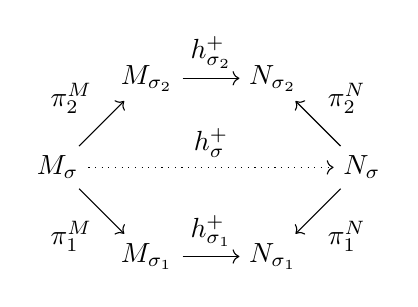
\begin{tikzpicture} 
   \node(1) {$M_\sigma$};
   \node(2) [below right of=1] {$M_{\sigma_1}$};
   \node(3) [right of =2] {$N_{\sigma_1}$};
   \node(4) [above right of=3] {$N_{\sigma}$};
   \node(5) [above right of=1] {$M_{\sigma_2}$};
   \node(6) [right of=5] {$N_{\sigma_2}$};
   \draw[->, dotted] (1) to node {$h^+_\sigma$} (4);
   \draw[->] (1) to node [swap] {$\pi_1^M$} (2);
   \draw[->] (2) to node {$h^+_{\sigma_1}$} (3);
   \draw[->] (4) to node {$\pi_1^N$} (3);
   \draw[->] (1) to node {$\pi_2^M$} (5);
   \draw[->] (5) to node {$h^+_{\sigma_2}$} (6);
   \draw[->] (4) to node [swap] {$\pi_2^N$} (6);
\end{tikzpicture} \] Let $m\in M_\sigma$. We define $h^+_\sigma(m)$ to
be the unique $n\in N_\sigma$ that satisfies both
$\pi_1^N(n)=h^+_{\sigma_1}\circ\pi_1^M(m)$ and
$\pi_2^N(n)=h^+_{\sigma_2}\circ\pi_2^M(m)$. We know that such an $n$
exists and is unique because $N$ is a model of $T^+$ and $T^+$ defines
the symbols $\sigma$, $\pi_1$, and $\pi_2$ to be a product sort. One
can verify that this definition of $h^+_\sigma$ makes the above
diagram commute.
%Using the fact that $h_{\sigma_1}$ and $h_{\sigma_2}$ are injective, one can verify that $h_\sigma$ must be injective too.

Suppose, on the other hand, that $T^+$ defines $\sigma$ as the subsort
of ``elements of sort $\sigma_1$ that are $\phi$.'' Let $i\in\Sigma^+$
be the inclusion map of arity $\sigma\rightarrow\sigma_1$ with
$\sigma_1\in\Sigma$. As above, the definition of $h^+_\sigma$ is
suggested by the following diagram.
\[ 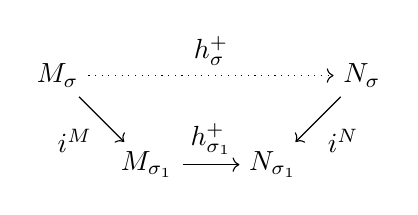
\begin{tikzpicture}
\node(1) {$M_\sigma$};
\node(2) [below right of=1] {$M_{\sigma_1}$};
\node(3) [right of =2] {$N_{\sigma_1}$};
\node(4) [above right of=3] {$N_{\sigma}$};
\draw[->, dotted] (1) to node  {$h^+_\sigma$} (4);
\draw[->] (1) to node [swap] {$i^M$} (2);
\draw[->] (2) to node {$h^+_{\sigma_1}$} (3);
\draw[->] (4) to node {$i^N$} (3);
\end{tikzpicture} \]
Let $m\in M_\sigma$. We see that following implications hold:
\begin{align*}
M\vDash\phi[i^M(m)]&\Rightarrow M|_\Sigma\vDash\phi[i^M(m)]\\
&\Rightarrow N|_\Sigma\vDash\phi[h^+_{\sigma_1}( i^M(m))]\Rightarrow N\vDash\phi[h^+_{\sigma_1}( i^M(m))]
\end{align*}
The first and third implications hold since $\phi(x)$ is a
$\Sigma$-formula, and the second holds because
$h_{\sigma_1}=h^+_{\sigma_1}$ and $h$ is an elementary
embedding. $T^+$ defines the symbols $i$ and $\sigma$ as a subsort and
$M$ is a model of $T^+$, so it must be that $M\vDash \phi[i^M(m)]$. By
the above implications, we see that
$N\vDash\phi[h^+_{\sigma_1}( i^M(m))]$. Since $N$ is also a model of
$T^+$, there is a unique $n\in N_\sigma$ that satisfies
$i^N(n)=h^+_{\sigma_1}(i^M(m))$. We define $h^+_\sigma(m)=n$. This
definition of $h^+_\sigma$ again makes the above diagram commute.

When $T^+$ defines $\sigma$ as a coproduct sort or a quotient sort one
describes the map $h^+_\sigma$ analogously.  We leave it to the reader
to work out the details of these cases.

For the purposes of proving Theorem \ref{mor1}, we need the following
simple lemma about this map $h^+$.

\begin{lemma} If $h:M|_\Sigma\rightarrow N|_\Sigma$ is an isomorphism,
  then $h^+:M\rightarrow N$ is an isomorphism. \label{lemmon}
\end{lemma}

\begin{proof} We know that $h_\sigma:M_\sigma\rightarrow N_\sigma$ is
  a bijection for each $\sigma\in\Sigma$. Using this fact and the
  definition of $h^+$, one can verify that
  $h^+_\sigma:M_\sigma\rightarrow N_\sigma$ is a bijection for each
  sort $\sigma\in\Sigma^+$. So $h^+$ is a family of bijections. And
  furthermore, the commutativity of the above diagrams implies that
  $h^+$ preserves any function
  symbols %$\pi_1,\pi_2, \rho_1,\rho_2, i,$ and $\epsilon$
  that are used to define new sorts.

  It only remains to check that $h^+$ preserves predicates, functions,
  and constants that have arities and sorts in $\Sigma$. Since
  $h:M|_\Sigma\rightarrow N|_\Sigma$ is a isomorphism, we know that
  $h^+$ preserves the symbols in $\Sigma$. So let
  $p\in\Sigma^+-\Sigma$ be a predicate symbol of arity
  $\sigma_1\times\ldots\times\sigma_n$ with
  $\sigma_1,\ldots,\sigma_n\in\Sigma$. There must be a
  $\Sigma$-formula $\phi(x_1,\ldots,x_n)$ such that
  $T^+\vDash\forall_{\sigma_1}x_1\ldots\forall_{\sigma_n}x_n(p(x_1,\ldots,x_n)\leftrightarrow\phi(x_1,\ldots,x_n))$. We
  know that $h:M|_\Sigma\rightarrow N|_\Sigma$ is an elementary
  embedding, so in particular it preserves the formula
  $\phi(x_1,\ldots, x_n)$. This implies that $(m_1,\ldots,m_n)\in p^M$
  if and only if
  $(h_{\sigma_1}(m_1),\ldots,h_{\sigma_n}(m_n))\in p^N$. Since
  $h^+_{\sigma_i}=h_{\sigma_i}$ for each $i=1,\ldots, n$, it must be
  that $h^+$ also preserves the predicate $p$. An analogous argument
  demonstrates that $h^+$ preserves functions and constants.
\end{proof}


%\begin{lemma}
%If $M$ and $N$ are models of $T^+$ and $M|_\Sigma\cong N|_\Sigma$, then $M\cong N$.
%\end{lemma}
%
%\begin{proof}
%Let $h:M|_\Sigma\rightarrow N|_\Sigma$ be an isomorphism. So $h$ is a family of maps $\{h_\sigma: M_\sigma\rightarrow N_\sigma\text{ such that } \sigma\in\Sigma\}$. For each new sort symbol $\sigma\in\Sigma^+-\Sigma$ we need to define $h_\sigma:M_\sigma\rightarrow N_\sigma$ and verify that the family of functions $h^+=\{h_\sigma: \sigma\in\Sigma^+\}$ is an isomorphism between $M$ and $N$. There are four cases, one for each way that the sort symbol $\sigma$ might be defined. We define $h_\sigma:M_\sigma\rightarrow N_\sigma$ in the cases where $\sigma$ is defined as a product sort and where $\sigma$ is defined as a subsort. The coproduct and quotient sort cases follow in an analogous manner.
%
%Suppose that $\sigma$ is defined as a product sort. We let $\pi_1,\pi_2\in\Sigma^+$ be the projections of arity $\sigma\rightarrow\sigma_1$ and $\sigma\rightarrow\sigma_2$, respectively, with $\sigma_1,\sigma_2\in\Sigma$ sort symbols. The definition of the function $h_\sigma$ is suggested by the following diagram.
%$$
%\begin{tikzpicture}
%\node(1) {$M_\sigma$};
%\node(2) [below right of=1] {$M_{\sigma_1}$};
%\node(3) [right of =2] {$N_{\sigma_1}$};
%\node(4) [above right of=3] {$N_{\sigma}$};
%\node(5) [above right of=1] {$M_{\sigma_2}$};
%\node(6) [right of=5] {$N_{\sigma_2}$};
%\draw[->, dotted] (1) to node  {$h_\sigma$} (4);
%\draw[->] (1) to node [swap] {$\pi_1^M$} (2);
%\draw[->] (2) to node {$h_{\sigma_1}$} (3);
%\draw[->] (4) to node {$\pi_1^N$} (3);
%\draw[->] (1) to node {$\pi_2^M$} (5);
%\draw[->] (5) to node {$h_{\sigma_2}$} (6);
%\draw[->] (4) to node [swap] {$\pi_2^N$} (6);
%\end{tikzpicture}
%$$
%If $a\in M_\sigma$ then we define $h_\sigma(a)$ to be the unique $b\in N_\sigma$ such that $\pi_1^N(b)=h_{\sigma_1}\circ\pi_1^M(a)$ and $\pi_2^N(b)=h_{\sigma_2}\circ\pi_2^M(a)$. We know that $b$ exists and is unique because $M$ is a model of $T^+$ and $T^+$ defines $\sigma$ as a product sort with projections $\pi_1$ and $\pi_2$. One can verify that $h_\sigma$ is a bijection.
%
%Suppose on the other hand that $\sigma$ is defined as a subsort with defining $\Sigma$-formula $\phi(x)$. Let $i\in\Sigma^+$ be the associated injection of arity $\sigma\rightarrow\sigma_1$ with $\sigma_1\in\Sigma$ a sort symbol. As above, the definition of $h_\sigma:M_\sigma\rightarrow N_\sigma$ is suggested by the following diagram.
%$$
%\begin{tikzpicture}
%\node(1) {$M_\sigma$};
%\node(2) [below right of=1] {$M_{\sigma_1}$};
%\node(3) [right of =2] {$N_{\sigma_1}$};
%\node(4) [above right of=3] {$N_{\sigma}$};
%\draw[->, dotted] (1) to node  {$h_\sigma$} (4);
%\draw[->] (1) to node [swap] {$i^M$} (2);
%\draw[->] (2) to node {$h_{\sigma_1}$} (3);
%\draw[->] (4) to node {$i^N$} (3);
%\end{tikzpicture}
%$$
%Suppose that $a\in M_\sigma$. Since $h:A|_\Sigma\rightarrow B_\Sigma$ is an isomorphism between these $\Sigma$-structures, it is an elementary embedding with respect to $\Sigma$-formulas. The following string of implications holds.
%\begin{align*}
%M\vDash\phi[i^M(a)]&\Rightarrow M|_\Sigma\vDash\phi[i^M(a)]\\
%&\Rightarrow N|_\Sigma\vDash\phi[h_{\sigma_1}( i^M(a))]\Rightarrow N\vDash\phi[h_{\sigma_1}( i^M(a))]
%\end{align*}
%The first and third implications follow from the fact that $\phi(x)$ is a $\Sigma$-formula, while the second follows from the fact that $h$ is an elementary embedding with respect to $\Sigma$-formulas. Since $M$ is a model of $T^+$ and $T^+$ defines $\sigma$ as a subsort, it must be that $M\vDash i^M(a)$. Because $N$ is also a model of $T^+$ this implies that there is a unique $b\in N_\sigma$ with $i^N(b)=h_{\sigma_1}\circ i^M(a)$. We define $h_\sigma(a)=b$ and one can verify that $h_\sigma$ is again a bijection.
%
%One defines $h_\sigma$ in an analogous manner when $\sigma$ is a coproduct or quotient sort. In both cases one then can then verify that $h_\sigma$ is a bijection. We have therefore defined a family of bijections $h^+=\{h_\sigma: \sigma\in\Sigma^+\}$. In order to demonstrate that $h^+$ is an isomorphism, we need only verify that it preserves predicates, functions, and constants. Since $h:M|_\Sigma\rightarrow N|_\Sigma$ is a isomorphism we know that $h^+$ preserves the symbols in $\Sigma$. Let $p\in\Sigma^+-\Sigma$ be a predicate symbol of arity $\sigma_1\times\ldots\times\sigma_n$ with $\sigma_1,\ldots,\sigma_n\in\Sigma$ sort symbols. We know that there is a $\Sigma$-formula $\phi(x_1,\ldots,x_n)$ such that $T^+\vDash\forall_{\sigma_1}x_1\ldots\forall_{\sigma_n}x_n(p(x_1,\ldots,x_n)\leftrightarrow\phi(x_1,\ldots,x_n))$. Using the fact that $h:M|_\Sigma\rightarrow N|_\Sigma$ is an elementary embedding with respect to $\Sigma$-formulas and the fact that $\phi(x_1,\ldots,x_n)$ is a $\Sigma$-formula, one can verify that $(a_1,\ldots,a_n)\in p^M$ if and only if $(h_{\sigma_1}(a_1),\ldots,h_{\sigma_n}(a_n))\in p^N$. So $h^+$ preserves the predicate $p$. One uses a similar argument to show that $h^+$ preserves function symbols and constant symbols. We conclude that $h^+:M\rightarrow N$ is an isomorphism.
%\end{proof}

We now turn to the proof of Theorem \ref{mor1}.

\begin{proof}[Proof of Theorem \ref{mor1}] Let $M$ be a model of
  $T$. First note that if $M^+$ exists, then it is unique up to
  isomorphism. For if $N$ is a model of $T^+$ with $N|_\Sigma=M$, then
  by letting $h$ be the identity map (which is an isomorphism) Lemma
  \ref{lemmon} implies that $M^+\cong N$. We need only define the
  $\Sigma^+$-structure $M^+$. To guarantee that $M^+$ is an expansion
  of $M$ we interpret every symbol in $\Sigma$ the same way that $M$
  does. We need to say how the symbols in $\Sigma^+\backslash\Sigma$
  are interpreted. There are a number of cases to consider.

  Suppose that $p\in\Sigma^+\backslash\Sigma$ is a predicate symbol of
  arity $\sigma_1\times\ldots\times\sigma_n$ with
  $\sigma_1,\ldots,\sigma_n\in\Sigma$. There must be a
  $\Sigma$-formula $\phi(x_1,\ldots, x_n)$ such that
  $T^+\vDash\forall_{\sigma_1}x_1\ldots\forall_{\sigma_n}x_n(p(x_1,\ldots,
  x_n)\leftrightarrow\phi(x_1,\ldots, x_n))$. We define the
  interpretation of the symbol $p$ in $M^+$ by letting
  $M^+(p)=M(\phi )$.  Obviously this definition implies that
  $M^+\vDash\delta_p$. The cases of function and constant symbols are
  handled similarly.

  Let $\sigma\in\Sigma^+\backslash\Sigma$ be a sort symbol. We
  describe the cases where $T^+$ defines $\sigma$ as a product sort or
  a subsort. The coproduct and quotient sort cases follow
  analogously. Suppose first that $\sigma$ is defined as a product
  sort with $\pi_1$ and $\pi_2$ the projections of arity
  $\sigma\rightarrow\sigma_1$ and $\sigma\rightarrow\sigma_2$,
  respectively. We define
  $M_\sigma^+=M^+_{\sigma_1}\times M^+_{\sigma_2}$ with
  $\pi_1^{M^+}:M^+_\sigma\rightarrow M^+_{\sigma_1}$ and
  $\pi_2^{M^+}:M^+_\sigma\rightarrow M^+_{\sigma_2}$ the canonical
  projections. One can easily verify that $M^+\vDash\delta_\sigma$. On
  the other hand, suppose that $\sigma$ is defined as a subsort with
  defining $\Sigma$-formula $\phi(x)$ and inclusion $i$ of arity
  $\sigma\rightarrow\sigma_1$. We define
  $M_\sigma^+=M(\phi )\subseteq M_{\sigma_1}$ with
  $i^{M^+}:M_\sigma^+\rightarrow M^+_{\sigma_1}$ the inclusion
  map. One can again verify that $M^+\vDash\delta_\sigma$.
%Since $M^+$ satisfies all of the definitions $\delta_s$, $M^+$ must be a model of $T^+$.
\end{proof}

The previous result immediately yields an important corollary:

\begin{thm}[Barrett] If $T^+$ is a Morita extension of $T$, then $T^+$
  is a conservative extension of $T$. \label{mor2}
\end{thm}

\begin{proof}
  Suppose that $T^+$ is not a conservative extension of $T$. One can
  easily see that $T\vdash\phi$ implies that $T^+\vdash\phi$ for every
  $\Sigma$-sentence $\phi$. So there must be some $\Sigma$-sentence
  $\phi$ such that $T^+\vdash\phi$, but $T\not\vdash\phi$. This
  implies that there is a model $M$ of $T$ such that
  $M\vDash\lnot\phi$. This model $M$ has no expansion that is a model
  of $T^+$ since $T^+\vdash\phi$, contradicting Theorem \ref{mor1}.
\end{proof}

Theorems \ref{mor1} and \ref{mor2} are natural generalizations from
definition extensions to Morita extensions.  In the case that $T^+$ is
a definitional extension of $T$, there are natural maps $I:T\to T^+$
and $R:T^+\to T$ that form a homotopy equivalence.  We now define a
reduction map $R:T^+\to T$ for the case where $T^+$ is a Morita
extension of $T$.

Lemma \ref{upstairs} shows that if $T^+$ is a definitional extension
of $T$ to $\Sigma^+$, then for every $\Sigma^+$-formula $\phi$ there
is a corresponding $\Sigma$-formula $R\phi$ such that
$T^+\vdash \phi\lra R\phi$.  The following example demonstrates that
this result does not generalize to the case of Morita extensions in a
perfectly straightforward manner.

\begin{example} Recall the theories $T$ and $T^+$ from Example
  \ref{extensionexample} and consider the $\Sigma^+$-formula
  $\phi(x, z)$ defined by $i(z)=x$. One can easily see that there is
  no $\Sigma$-formula $\phi^*(x, z)$ that is equivalent to
  $\phi(x, z)$ according to the theory $T^+$. Indeed, the variable $z$
  cannot appear in any $\Sigma$-formula since it is of sort
  $\sigma^+\in\Sigma^+\backslash\Sigma$. A $\Sigma$-formula simply
  cannot say how variables with sorts in $\Sigma$ relate to variables
  with sorts in $\Sigma^+$.
\end{example}

In order to define $R:T^+\to T$, therefore, we need a way of
specifying how variables with sorts in $\Sigma^+\backslash\Sigma$
relate to variables with sorts in $\Sigma$.  We do this by defining
the concept of a ``code'' \cite[see][]{szczerba1977}.

\begin{defn} Let $\Sigma\subseteq\Sigma^+$ be signatures with $T$ a
  $\Sigma$-theory and $T^+$ a Morita extension of $T$ to $\Sigma^+$.
  We define a \emph{code} formula $\xi (x,y_1,y_2)$ for each variable
  $x$ of sort $\sigma\in\Sigma^+\backslash\Sigma$ as follows:
  \begin{itemize}
  \item Suppose that $T^+$ defines $\sigma$ as a product sort with
    $\pi_1$ and $\pi_2$ the corresponding projections.  Then
    $\xi (x,y_1,y_2)$ is the $\Sigma ^+$-formula
    \[ (y_1=\pi _1(x))\wedge (y_2=\pi _2(x)) .\]
  \item Suppose that $T^+$ defines $\sigma$ as a coproduct sort with
    corresponding function symbols $\rho_1:\sigma _1\to\sigma$ and
    $\rho_2:\sigma _2\to\sigma$.  Then $\xi (x,y_1,y_2)$ is either the
    $\Sigma^+$-formula $\rho_1(y_1)=x$ or the $\Sigma^+$-formula
    $\rho_2(y_2)=x$, where $y_i$ is a variable of sort $\sigma _i$.
    (Note: $\xi (x,y_1,y_2)$ is {\it not} the disjunction of these two
    formulas.)
  \item Suppose that $T^+$ defines $\sigma$ as a subsort with
    $i:\sigma\to\sigma '$ the corresponding function symbol.  Then
    $\xi (x,y)$ is the formula $i(x)=y$, where $y$ is a variable of
    sort $\sigma '\in\Sigma$.
  \item Suppose that $T^+$ defines $\sigma$ as a quotient sort with
    $\epsilon :\sigma '\rightarrow\sigma$ the corresponding function
    symbol. Then $\xi (x,y)$ is the $\Sigma^+$-formula
    $\epsilon(y)=x$, where $y$ is again a variable of sort
    $\sigma '\in\Sigma$.
  \item Given the empty sequence of variables, we let the
    \textbf{empty code} be the tautology $\exists x(x=_\sigma x)$,
    where $\sigma\in\Sigma$ is a sort symbol.
  \end{itemize}

  Given the conjuncts $\xi _1,\dots ,\xi _n$, we will use the notation
  $\xi(x_1, \ldots, y_{n2})$ to denote the code
  $\xi_1(x_1,y_{11}, y_{12})\land\ldots\land\xi_n(x_n, y_{n1},
  y_{n2})$ for the variables $x_1,\ldots, x_n$.  Note that the
  variables $y_{i1}$ and $y_{i2}$ have sorts in $\Sigma$ for each
  $i=1,\ldots, n$. One should think of a code
  $\xi(x_1,\ldots, y_{n2})$ for $x_1,\ldots, x_n$ as encoding one way
  that the variables $x_1,\ldots, x_n$ with sorts in
  $\Sigma^+\backslash\Sigma$ might be related to variables
  $y_{11}, \ldots, y_{n2}$ that have sorts in $\Sigma$. One additional
  piece of notation will be useful in what follows. Given a
  $\Sigma^+$-formula $\phi$, we will write
  $\phi(x_1,\ldots, x_n, \overline{x}_1, \ldots, \overline{x}_m)$ to
  indicate that the variables $x_1,\ldots, x_n$ have sorts
  $\sigma_1,\ldots, \sigma_n\in\Sigma^+\backslash\Sigma$ and that the
  variables $\overline{x}_1,\ldots, \overline{x}_m$ have sorts
  $\overline{\sigma}_1,\ldots,
  \overline{\sigma}_m\in\Sigma$. \end{defn}


\begin{lemma}[Functionality of codes] Let $T$ be a $\Sigma$-theory and
  $T^+$ a Morita extension of $T$ to the signature $\Sigma ^+$.  Let
  $\vec{x},\vec{z}$ be $n$-tuples of variables of the same sorts in
  $\Sigma ^+$ and let $\xi (\vec{x},\vec{y})$ be a code for $\vec{x}$.
  Then we have
  \[ T^+ \: \vdash \: (\xi (\vec{x},\vec{y})\wedge \xi
    (\vec{z},\vec{y}))\to \vec{x}=\vec{z} ,\] where $\vec{x}=\vec{z}$ is
  shorthand for
  $(x_1=_{\sigma _1}z_1)\wedge\cdots\wedge (x_n=_{\sigma
    _n}z_n)$. \end{lemma}


\begin{proof} This fact follows immediately from the definition of
  codes.
\end{proof}

We can now state our generalization of Lemma \ref{upstairs}.  

\begin{thm}[Barrett] Let $\Sigma\subseteq\Sigma^+$ be signatures and
  $T$ a $\Sigma$-theory. Suppose that $T^+$ is a Morita extension of
  $T$ to $\Sigma^+$ and that
  $\phi(x_1,\ldots, x_n, \overline{x}_1,\ldots, \overline{x}_m)$ is a
  $\Sigma^+$-formula. Then for every code $\xi(x_1,\ldots, y_{n2})$
  for the variables $x_1,\ldots, x_n$ there is a $\Sigma$-formula
  $\phi^*(\overline{x}_1,\ldots, \overline{x}_m, y_{11}, \ldots,
  y_{n2})$ such that $T^+$ entails
  \[ \xi(x_1,\ldots, y_{n2})\rightarrow (\phi(x_1,\ldots x_n,
    \overline{x}_1,\ldots,
    \overline{x}_m)\leftrightarrow\phi^*(\overline{x}_1,\ldots,\overline{x}_m,
    y_{11},\ldots, y_{n2})) .
\] \label{mor4}
\end{thm}

The idea behind Theorem \ref{mor4} is simple. Although one might not
initially be able to translate a $\Sigma^+$-formula $\phi$ into an
equivalent $\Sigma$-formula $\phi^*$, such a translation is possible
after one specifies how the variables in $\phi$ with sorts in
$\Sigma^+-\Sigma$ are related to variables with sorts in $\Sigma$.

We first prove the following lemma. Given a $\Sigma^+$-term $t$, we
will again write
$t(x_1,\ldots, x_n,\overline{x}_1,\ldots, \overline{x}_m)$ to indicate
that the variables $x_1,\ldots, x_n$ have sorts
$\sigma_1,\ldots, \sigma_n\in\Sigma^+\backslash\Sigma$ and that the
variables $\overline{x}_1,\ldots, \overline{x}_m$ have sorts
$\overline{\sigma}_1,\ldots, \overline{\sigma}_m\in\Sigma$.

\begin{lemma} Let
  $t(x_1,\ldots, x_n, \overline{x}_1,\ldots, \overline{x}_m)$ be a
  $\Sigma^+$-term of sort $\sigma$ and $x$ a variable of sort
  $\sigma$. Let
  $\xi(x,x_1,\ldots, x_n,y_1,y_2,y_{11}, \ldots, y_{n2})$ be a code
  for the variables $x,x_1,\ldots, x_n$, where the variables $y_1$ and
  $y_2$ are used for coding the variable $x$.  Then there is a
  $\Sigma$-formula
  $\phi_t(x,\overline{x}_1,\ldots, \overline{x}_m, y_{01}, \ldots,
  y_{n2})$ such that $T^+$ implies 
  \[ \xi(x,\ldots, y_{n2})\rightarrow \big(t(x_1, \ldots,
    \overline{x}_m)=x\leftrightarrow\phi_t(x,
    \overline{x}_1,\ldots,\overline{x}_m, y_1,\ldots, y_{n2})\big)
    . \] If $\sigma\in\Sigma$, then $x$ will not appear in the code
  $\xi$. If $\sigma\in\Sigma^+\backslash\Sigma$, then $x$ will not
  appear in the $\Sigma$-formula $\phi_t$. \label{thomas} \end{lemma}

\begin{proof} We induct on the complexity of $t$. First, suppose that
  $t$ is a variable $x_i$ of sort $\sigma$.  If $\sigma\in\Sigma$,
  then there are no variables in $t$ with sorts in
  $\Sigma^+\backslash\Sigma$. So $\xi$ must be the empty code. Let
  $\phi_t(x, x_i)$ be the $\Sigma$-formula $x=x_i$. This choice of
  $\phi_t$ trivially satisfies the desired property. If
  $\sigma\in\Sigma^+\backslash\Sigma$, then there are four cases to
  consider. We consider the cases where $\sigma$ is a product sort and
  a subsort. The coproduct and quotient cases follow
  analogously. Suppose that $T^+$ defines $\sigma$ as a product sort
  with projections $\pi_1$ and $\pi_2$ of arity
  $\sigma\rightarrow\sigma_1$ and $\sigma\rightarrow\sigma_2$. A code
  $\xi$ for the variables $x$ and $x_i$ must therefore be the formula
\[
  \pi_1(x)=y_1\land\pi_2(x)=y_2\land\pi_1(x_i)=y_{i1}\land\pi_2(x_i)=y_{i2}
  .\] One defines the $\Sigma$-formula $\phi_t$ to be
$y_1=y_{i1}\land y_2=y_{i2}$ and verifies that it satisfies the
desired property. On the other hand, suppose that $T^+$ defines
$\sigma$ as a subsort with injection $i$ of arity
$\sigma\rightarrow\sigma_1$. A code $\xi$ for the variables $x$ and
$x_i$ is therefore the formula \[ i(x)=y\land i(x_i)=y_{i1} .\] Let
$\phi_t$ be the $\Sigma$-formula $y=y_{i1}$. The desired property
again holds.

Second, suppose that $t$ is the constant symbol $c$. Note that it must
be the case that $c$ is of sort $\sigma\in\Sigma$. If $c\in\Sigma$,
then letting $\phi_t$ be the $\Sigma$-formula $x=c$ trivially yields
the result. If $c\in\Sigma^+\backslash\Sigma$, then there is some
$\Sigma$-formula $\psi(x)$ that $T^+$ uses to explicitly define
$c$. Letting $\phi_t=\psi$ yields the desired result.

For the third (and final) step of the induction, we suppose that $t$ is a term of the form
\[ f\big(t_1(x_1,\ldots, x_n, \overline{x}_1,\ldots, \overline{x}_m),
  \ldots, t_k(x_1,\ldots, x_n, \overline{x}_1,\ldots,
  \overline{x}_m)\big) \] where $f\in\Sigma^+$ is a function
symbol. We show that the result holds for $t$ if it holds for all of
the terms $t_1,\ldots, t_k$. There are three cases to consider. First,
if $f\in\Sigma$, then it must be that $f$ has arity
$\sigma_1\times\ldots\times\sigma_k\rightarrow\sigma$, where
$\sigma,\sigma_1,\ldots, \sigma_k\in\Sigma$. Let $\xi$ be a code for
$x_1,\ldots, x_n$. We define $\phi_t$ to be the $\Sigma$-formula
\[ \exists_{\sigma_1}
  z_1\ldots\exists_{\sigma_k}z_k\big(\phi_{t_1}(z_1,
  \overline{x}_1,\ldots, y_{n2})\land\ldots\land\phi_{t_k}(z_k,
  \overline{x}_1,\ldots y_{n2})\land f(z_1,\ldots, z_k)=x\big) .\]
where each of the $\phi_{t_i}$ exists by our inductive hypothesis. One
can verify that $\phi_t$ satisfies the desired property. Second, if
$f\in\Sigma^+\backslash\Sigma$ is defined by a $\Sigma$-formula
$\psi(z_1,\ldots, z_k, x)$ then one defines $\phi_t$ in an analogous
manner to above. (Note that in this case the arity of $f$ is again
$\sigma_1\times\ldots\times\sigma_k\rightarrow \sigma$ with
$\sigma_1,\ldots, \sigma_k,\sigma\in\Sigma$.)

Third, we need to verify that the result holds if $f$ is a function
symbol that is used in the definition of a new sort. We discuss the
cases where $f$ is $\pi_1$ and where $f$ is $\epsilon$. Suppose that
$f$ is $\pi_1$ with arity $\sigma\rightarrow\sigma_1$. Then it must be
that the term $t_1$ is a variable $x_i$ of sort $\sigma$ since there
are no other $\Sigma^+$-terms of sort $\sigma$. So the term $t$ is
$\pi_1(x_i)$. Let $\xi(x_i, y_{i1}, y_{i2})$ be a code for $x_i$. It
must be that $\xi$ is the formula
\[  \pi_1(x_i)=y_{i1}\land\pi_2(x_i)=y_{i2} . \]
Letting $\phi_t$ be the formula $y_{i1}=x$ yields the desired
result. On the other hand, suppose that $f$ is the function symbol
$\epsilon$ of arity $\sigma_1\rightarrow\sigma$, where $\sigma$ is a
quotient sort defined by the $\Sigma$-formula $\psi(z_1, z_2)$. The
term $t$ in this case is
$\epsilon(t_1(x_1,\ldots, x_n, \overline{x}_1,\ldots,
\overline{x}_m))$ and we assume that the result holds for the
$\Sigma^+$-term $t_1$ of sort $\sigma_1\in\Sigma$. Let $\xi$ be a code
for the variables $x, x_1,\ldots, x_n$. This code determines a code
$\overline{\xi}$ for the variables $x_1,\ldots, x_n$ by ``forgetting''
the conjunct $\epsilon(y)=x$ that involves the variable $x$. We use
the code $\overline{\xi}$ and the inductive hypothesis to obtain the
formula $\phi_{t_1}$. Then we define $\phi_t$ to be the
$\Sigma$-formula
\[ \exists_{\sigma_1} z\big(\phi_{t_1}(z, \overline{x}_1,\ldots,
\overline{x}_m, y_{11},\ldots, y_{n2})\land\psi(y, z)\big) \]
Considering the original code $\xi$, one verifies that the result holds for $\phi_{t_1}$.
\end{proof}

We now turn to the proof of the main result.

\begin{proof} We induct on the complexity of $\phi$. Suppose that
  $\phi$ is the formula
  $t(x_1,\ldots, x_n, \overline{x}_1,\ldots,
  \overline{x}_m)=s(x_1,\ldots, x_n,
  \overline{x}_1,\ldots,\overline{x}_m)$ where $t$ and $s$ are
  $\Sigma^+$-terms of sort $\sigma$.  Let $\xi(x_1,\ldots, y_{n2})$ be
  a code for $x_1,\ldots, x_n$ and let $x$ be a variable of sort
  $\sigma$.  By Lemma \ref{thomas}, there are corresponding
  $\Sigma$-formulas
  $\phi_t(x,\overline{x}_1,\ldots, \overline{x}_m, y_{11}, \ldots,
  y_{n2})$ and
  $\phi_s(x,\overline{x}_1,\ldots, \overline{x}_m, y_{11}, \ldots,
  y_{n2})$.  The $\Sigma$-formula $\phi^*$ is then defined to be
\[ 
  \exists_\sigma x\big(\phi_t(x,\overline{x}_1,\ldots, \overline{x}_m,
  y_{11}, \ldots, y_{n2})\land\phi_s(x,\overline{x}_1,\ldots,
  \overline{x}_m, y_{11}, \ldots, y_{n2})\big) . \] One can verify
that this definition of $\phi^*$ satisfies the desired result.

If $t$ and $s$ are of sort $\sigma\in\Sigma^+\backslash\Sigma$, then
there are four cases to consider. We show that the result holds when
$T^+$ defines $\sigma$ as a product sort or a quotient sort. The
coproduct and subsort cases follow analogously. If $T^+$ defines
$\sigma$ as a product sort with projections $\pi_1$ and $\pi_2$ of
arity $\sigma\rightarrow\sigma_1$ and $\sigma\rightarrow\sigma_2$,
then we define a code
$\overline{\xi}(x, x_1,\ldots, y_{n2}, v_1, v_2)$ for the variables
$x, x_1,\ldots, x_n$ by
\[ \xi(x_1,\ldots, y_{n2})\land\pi_1(x)=v_1\land\pi_2(x)=v_2 .\] Lemma
\ref{thomas} and the code $\overline{\xi}$ for the variables
$x,x_1,\ldots, x_n$ generate the $\Sigma$-formulas
$\phi_t(\overline{x}_1,\ldots, \overline{x}_m, y_{11}, \ldots, y_{n2},
v_1, v_2)$ and
$\phi_s(\overline{x}_1,\ldots, \overline{x}_m, y_{11}, \ldots, y_{n2},
v_1, v_2)$. We then define the $\Sigma$-formula $\phi^*$ to be
\begin{align*}
\exists_{\sigma_1}v_1\exists_{\sigma_2}v_2\big(&\phi_t(\overline{x}_1,\ldots, \overline{x}_m, y_{11}, \ldots, y_{n2}, v_1, v_2)\\ 
&\land \phi_s(\overline{x}_1,\ldots, \overline{x}_m, y_{11}, \ldots, y_{n2}, v_1, v_2)\big)
\end{align*}
One can verify that $\phi^*$ again satisfies the desired result. 

If $T^+$ defines $\sigma$ as a quotient sort with projection
$\epsilon$ of arity $\sigma_1\rightarrow\sigma$, then we again define
a new code $\overline{\xi}(x, x_1,\ldots, y_{n2}, v)$ for the
variables $x, x_1,\ldots, x_n$ by
$$
\xi(x_1,\ldots, y_{n2})\land\epsilon(v)=x
$$
Lemma \ref{thomas} and the code $\overline{\xi}$ for the variables
$x, x_1,\ldots, x_n$ again generate the $\Sigma$-formulas
$\phi_t(\overline{x}_1,\ldots, \overline{x}_m, y_{11}, \ldots, y_{n2},
v)$ and
$\phi_s(\overline{x}_1,\ldots, \overline{x}_m, y_{11}, \ldots, y_{n2},
v)$. We define the $\Sigma$-formula $\phi^*$ to be
\[ \exists_{\sigma_1} v \big(\phi_t(\overline{x}_1,\ldots,
  \overline{x}_m, y_{11}, \ldots, y_{n2}, v)\land
  \phi_s(\overline{x}_1,\ldots, \overline{x}_m, y_{11}, \ldots,
  y_{n2}, v)\big) \] One again verifies that this $\phi^*$ satisfies
the desired property. So the result holds when $\phi$ is of the form
$t=s$ for $\Sigma^+$-terms $t$ and $s$.

Now suppose that $\phi(x_1,\ldots, x_n,\overline{x}_1,\ldots, \overline{x}_m)$ is a $\Sigma^+$-formula of the form 
\[ p(t_1(x_1,\ldots, x_n,\overline{x}_1,\ldots,\overline{x}_m),\ldots,
  t_k(x_1,\ldots, x_n, \overline{x}_1,\ldots, \overline{x}_m)) \]
where $p$ has arity $\sigma_1\times\ldots\times\sigma_k$. Note that it
must be that $\sigma_1,\ldots,\sigma_k\in\Sigma$. Either $p\in\Sigma$
or $p\in\Sigma^+\backslash\Sigma$. We consider the second case. (The
first is analogous.) Let $\psi(z_1,\ldots, z_k)$ be the
$\Sigma$-formula that $T^+$ uses to explicitly define $p$ and let
$\xi(x_1,\ldots, y_{n2})$ be a code for $x_1,\ldots, x_n$. Lemma
\ref{thomas} and $\xi$ generate the $\Sigma$-formulas
$\phi_{t_i}(z_i, \overline{x}_1,\ldots, \overline{x}_m, y_{11},
\ldots, y_{n2})$ for each $i=1,\ldots, k$. We define $\phi^*$ to be
the $\Sigma$-formula
\begin{align*}
\exists_{\sigma_1}z_1\ldots\exists_{\sigma_k}z_k\big(&\phi_{t_1}(z_1,\overline{x}_1,\ldots, \overline{x}_m,y_{11},\ldots, y_{n2})\land\ldots\\ &\land\phi_{t_k}(z_k,\overline{x}_1,\ldots, \overline{x}_m,y_{11},\ldots, y_{n2})\land\psi(z_1,\ldots, z_k)\big)
\end{align*}
One can again verify that the result holds for this choice of
$\phi^*$.

We have covered the ``base cases'' for our induction. We now turn to
the inductive step. We consider the cases of $\lnot, \land$, and
$\forall$. Suppose that the result holds for $\Sigma^+$-formulas
$\phi_1$ and $\phi_2$. Then it trivially holds for $\lnot\phi_1$ by
letting $(\lnot\phi)^*$ be $\lnot(\phi^*)$. It also trivially holds
for $\phi_1\land\phi_2$ by letting $(\phi_1\land\phi_2)^*$ be
$\phi_1^*\land\phi_2^*$.

The $\forall_{\sigma_i}$ case requires more work. If $x_i$ is a
variable of sort $\sigma_i\in\Sigma$, we let
$(\forall_{\sigma_i} x_i \phi_1)^*$ be
$\forall_{\sigma_i} x_i (\phi_1^*)$. The only non-trivial part of the
inductive step is when one quantifies over variables with sorts in
$\Sigma^+\backslash\Sigma$. Suppose that
$\phi(x_1,\ldots, x_n, \overline{x}_1,\ldots, \overline{x}_m)$ is a
$\Sigma^+$-formula and that the result holds for it. We let $x_i$ be a
variable of sort $\sigma_i\in\Sigma^+\backslash\Sigma$ and we show
that the result also holds for the $\Sigma$-formula
$\forall_{\sigma_i}x_i\phi(x_1,\ldots, x_n, \overline{x}_1,\ldots,
\overline{x}_m)$. There are again four cases. We show that the result
holds when $\sigma_i$ is a product sort and a coproduct sort. The
cases of subsorts and quotient sorts follow analogously.

Suppose that $T^+$ defines $\sigma_i$ as a product sort with
projections $\pi_1$ and $\pi_2$ of arity
$\sigma_i\rightarrow\sigma_{i1}$ and $\sigma_i\rightarrow\sigma_{i2}$.
Quantifying over a variable $x_i$ of product sort $\sigma_i$ can be
thought of as ``quantifying over pairs of elements of sorts
$\sigma_{i1}$ and $\sigma_{i2}$.''  Indeed, let
$\xi(x_1,\ldots, y_{n2})$ be a code for the variables
$x_1,\ldots, x_{i-1}, x_{i+1}, \ldots, x_n$ (these are all of the free
variables in $\forall_{\sigma_i}x_i\phi$ with sorts in
$\Sigma^+\backslash\Sigma$). We define a code $\overline{\xi}$ for the
variables $x_1,\ldots, x_{i-1}, x_i, x_{i+1}, \ldots, x_n$ by
\[ \xi(x_1,\ldots, y_{n2})\land\pi_1(x_i)=v_1\land\pi_2(x_i)=v_2 .\]
One uses the code $\overline{\xi}$ and the inductive hypothesis to
generate the $\Sigma$-formula
$\phi^*(\overline{x}_1,\ldots, \overline{x}_m, y_{11},\ldots, y_{n2},
v_1, v_2)$. We then define the $\Sigma$-formula
$(\forall_{\sigma_i}x_i\phi)^*$ to be
\[ \forall_{\sigma_{i1}}
  v_1\forall_{\sigma_{i2}}v_2\phi^*(\overline{x}_1,\ldots,
  \overline{x}_m, y_{11},\ldots, y_{n2}, v_1, v_2) .\]
And one verifies that the desired result holds for this choice of
$(\forall_{\sigma_i}x_i\phi)^*$.

Suppose that $T^+$ defines $\sigma_i$ as a coproduct sort with
injections $\rho_1$ and $\rho_2$ of arity
$\sigma_{i1}\rightarrow\sigma_{i}$ and
$\sigma_{i2}\rightarrow\sigma_i$.  Quantifying over a variable $x_i$
of coproduct sort $\sigma_i$ can be thought of as ``quantifying over
\textit{both} elements of sort $\sigma_{i1}$ and elements of sort
$\sigma_{i2}$.''  Indeed, let $\xi(x_1,\ldots, y_{n2})$ be a code for
the variables $x_1,\ldots, x_{i-1}, x_{i+1}, \ldots, x_n$ (these are
again all of the free variables in $\forall_{\sigma_i}x_i\phi$ with
sorts in $\Sigma^+-\Sigma$). We define two different codes
$\overline{\xi}$ for the variables
$x_1,\ldots, x_{i-1}, x_i, x_{i+1}, \ldots, x_n$ by
\begin{gather*}
\xi(x_1,\ldots, y_{n2})\land\rho_1(v_1)=x_i\\
\xi(x_1,\ldots, y_{n2})\land\rho_2(v_2)=x_i
\end{gather*}
We will call the first code $\xi'(x_1,\ldots, y_{n2}, v_1)$ and the
second $\xi''(x_1,\ldots, y_{n2}, v_2)$. We use these two codes and
the inductive hypothesis to generate $\Sigma$-formulas $\phi^{*'}$ and
$\phi^{*''}$. We then define the $\Sigma$-formula
$(\forall_{\sigma_i}x_i\phi)^*$ to be
\begin{align*}
  \forall_{\sigma_{i1}}v_1\forall_{\sigma_{i2}}v_2\big(&\phi^{*'}(\overline{x}_1,\ldots,\overline{x}_m,y_{11}, \ldots, y_{n2}, v_2)\\
                                                       &\land\phi^{*''}(\overline{x}_1,\ldots, \overline{x}_m,y_{11},\ldots, y_{n2}, v_2)\big)
\end{align*}
One can verify that the desired result holds again for this definition
of $(\forall_{\sigma_i}x_i\phi)^*$.
\end{proof}

Theorem \ref{mor4} has the following immediate corollary.

\begin{cor} Let $\Sigma\subseteq\Sigma^+$ be signatures and $T$ a
  $\Sigma$-theory. If $T^+$ is a Morita extension of $T$ to
  $\Sigma^+$, then for every $\Sigma^+$-sentence $\phi$ there is a
  $\Sigma$-sentence $\phi^*$ such that
  $T^+\vdash\phi\leftrightarrow\phi^*$. \label{morph}
\end{cor}

\begin{proof} Let $\phi$ be a $\Sigma^+$-sentence and consider the
  empty code $\xi$.  Theorem \ref{mor4} implies that there is a
  $\Sigma$-sentence $\phi^*$ such that
  $T^+\vdash \xi\rightarrow (\phi\leftrightarrow\phi^*)$. Since $\xi$
  is a tautology we trivially have that
  $T^+\vdash\phi\leftrightarrow\phi^*$.
\end{proof}

The theorems in this section capture different senses in which a
Morita extension of a theory ``says no more'' than the original
theory. In this way, Morita equivalence is analogous to definitional
equivalence.

At first glance, Morita equivalence might strike one as different from
definitional equivalence in an important way. To show that theories
are Morita equivalent, one is allowed to take any finite number of
Morita extensions of the theories. On the other hand, to show that two
theories are definitionally equivalent, it appears that one is only
allowed to take \textit{one} definitional extension of each
theory. One might worry that Morita equivalence is therefore not
perfectly analogous to definitional equivalence.

Fortunately, this is not the case. Theorem 3.3 implies that if
theories $T_1, \ldots, T_n$ are such that each $T_{i+1}$ is a
definitional extension of $T_i$, then $T_n$ is in fact a definitional
extension of $T_1$. (One can easily verify that this is not true of
Morita extensions.) To show that two theories are definitionally
equivalent, therefore, one actually \textit{is} allowed to take any
finite number of definitional extensions of each theory.

If two theories are definitionally equivalent, then they are trivially
Morita equivalent. Unlike definitional equivalence, however, Morita
equivalence is capable of capturing a sense in which theories with
different sort symbols are equivalent.  The following example
demonstrates that Morita equivalence is a more liberal criterion for
theoretical equivalence.

\begin{example}
  Let $\Sigma _1 =\{ \sigma _1,p,q\}$ and
  $\Sigma _2=\{ \sigma _2,\sigma _3 \}$ be signatures with $\sigma _i$
  sort symbols, and $p$ and $q$ predicate symbols of arity
  $\sigma _1$.  Let $T_1$ be the $\Sigma_1$-theory that says: $p$ and
  $q$ are non-empty, mutually exclusive, and exhaustive.  Let $T_2$ be
  the empty theory in $\Sigma _2$.  Since the signatures $\Sigma _1$
  and $\Sigma _2$ have different sort symbols, $T_1$ and $T_2$ can't
  possibly be definitionally equivalent.  Nonetheless, it's easy to
  see that $T_1$ and $T_2$ are Morita equivalent. Let
  $\Sigma=\Sigma_1\cup\Sigma_2\cup\{i_2, i_3\}$ be a signature with
  $i_2$ and $i_3$ function symbols of arity
  $\sigma_2\rightarrow\sigma_1$ and
  $\sigma_3\rightarrow\sigma_1$. Consider the following
  $\Sigma$-sentences.
\begin{align*}
%
&\begin{aligned}
&\forall_{\sigma_1}x\big(p(x)\leftrightarrow\exists_{\sigma_2} y(i_2(y)=x)\big)\\
&\qquad\land\forall_{\sigma_2} y_1\forall_{\sigma_2} y_2\big(i_2(y_1)=i_2(y_2)\rightarrow y_1=y_2\big)\\
\end{aligned}
\tag{$\delta_{\sigma_2}$}\\
%
&\begin{aligned}
&\forall_{\sigma_1}x\big(q(x)\leftrightarrow\exists_{\sigma_3} z(i_3(z)=x)\big)\\
&\qquad\land\forall_{\sigma_3} z_1\forall_{\sigma_3} z_2\big(i_3(z_1)=i_3(z_2)\rightarrow z_1=z_2\big)\\
\end{aligned}
\tag{$\delta_{\sigma_3}$}\\
&\begin{aligned}
&\forall_{\sigma_1} x\big(\exists_{\sigma_2=1}y(i_2(y)=x)\lor\exists_{\sigma_3=1} z(i_3(z)=x)\big)\\
&\qquad\land \forall_{\sigma_2} y\forall_{\sigma_3} z \lnot\big(i_2(y)=i_3(z)\big)\\
\end{aligned}
\tag{$\delta_{\sigma_1}$}\\
&\begin{aligned}
&\forall_{\sigma_1} x\big(p(x)\leftrightarrow\exists_{\sigma_2} y(i_2(y)=x)\big)
\end{aligned} 
\tag{$\delta_p$}\\
%
&\begin{aligned}
&\forall_{\sigma_1} x\big(q(x)\leftrightarrow\exists_{\sigma_3} z(i_3(z)=x)\big)
\end{aligned}
\tag{$\delta_q$}
\end{align*}
The $\Sigma$-theory
$T_1^1=T_1\cup\{\delta_{\sigma_2}, \delta_{\sigma_3}\}$ is a Morita
extension of $T_1$ to the signature $\Sigma$.  It defines $\sigma_2$
to be the subsort of ``elements that are $p$'' and $\sigma_3$ to be
the subsort of ``elements that are $q$.''

The theory $T_2^1=T_2\cup\{\delta_{\sigma_1}\}$ is a Morita extension
of $T_2$ to the signature $\Sigma_2\cup\{\sigma_1, i_2, i_3\}$. It
defines $\sigma_1$ to be the coproduct sort of $\sigma_2$ and
$\sigma_3$. Lastly, the $\Sigma$-theory
$T_2^2=T_2^1\cup\{\delta_p, \delta_q\}$ is a Morita extension of
$T_2^1$ to the signature $\Sigma$. It defines the predicates $p$ and
$q$ to apply to elements in the ``images'' of $i_2$ and $i_3$,
respectively.  One can verify that $T_1^1$ and $T_2^2$ are logically
equivalent, so $T_1$ and $T_2$ are Morita equivalent.
\end{example}

Morita equivalence captures a clear and robust sense in which theories
might be equivalent, but it is a difficult criterion to apply outside
of the framework of first-order logic. Indeed, without a formal
language one does not have the resources to say what an explicit
definition is. Questions of equivalence and inequivalence of theories,
however, still come up outside of this framework. It is well known,
for example, that there are different ways of formulating the theory
of smooth manifolds \citep{nestruev2002}. There are also different
formulations of the theory of topological spaces
\citep{kuratowski1966}.  None of these formulations are first-order
theories.  Physical theories too are rarely formulated in first-order
logic, and there are many pairs of physical theories that have been
considered to be equivalent.  We list just a few examples.

\begin{itemize}
\item According to the standard view in physics, Heisenberg's matrix
  mechanics is equivalent to Schr{\"o}dinger's wave mechanics ---
  despite the fact that these theories use completely different
  formalisms, and neither is axiomatizable in first-order logic.  Or,
  if you prefer to be more mathematically rigorous, quantum mechanics
  can be formulated either in terms of Hilbert spaces, or in terms of
  $C^*$-algebras.  There are good reasons, however, to think that
  these two formulations are equivalent.
\item Einstein's general theory of relativity is typically formulated
  in terms of differential geometry.  However, we have a free choice:
  either we can use a metric of signature $(3,1)$ or a metric of
  signature $(1,3)$.  The two formulations of GTR seem to be
  equivalent --- but it's hard to see how we could explicate that
  equivalence in terms of some regimentation of these theories in
  first-order logic.

  Even more extremely, it's also possible to reformulate GTR as an
  algebraic theory, rather than as a spatial theory.  However, there
  are good reasons to believe that the algebraic and spatial
  formulations of GTR are equivalent
  \citep[see][]{rosenstock,weatherall2015}.
  
\item GTR seems to be fundamentally different in kind from classical
  Newtonian gravitation, since the latter posits a static spacetime
  structure.  Some have claimed in fact that GTR has a special
  property, called ``general covariance,'' that disguishes it from all
  previous spacetime theories.  However, in the mid 20th century,
  Henri Cartan formulated a coordinate free version of Newtonian
  gravitation on a curved spacetime.  If this Newton-Cartan
  gravitational theory is equivalent to Newtonian gravity, then the
  latter is also generally covariant.  For discussion of this example,
  see \cite{glymour1977,knox2013,weatherall-erk}.

\item In typical presentations of rigorous methods in classical
  physics, it is usually assumed (or even partially demonstrated) that
  the Lagrangian formalism is equivalent to the Hamiltonian formalism.
  However, \cite{north2009} argues that these two theories have
  different structure, and hence are inequivalent.  For further
  discussion, see
  \cite{halvorsonunpublished,swansonhalvorsonunpublished,curiel2014,barrett2014}.

\item Most cutting-edge theories in physics make use of the so-called
  gauge formalism, and this raises many challenging interpretive
  issues \citep[see][]{healey-gauge}.  Philosophers of science have
  recently entered into a dispute about whether gauge theories are
  better thought of in terms of the fiber bundle formalism, or in
  terms of the holonomy formalism.  However, \cite{rosenstock2016}
  argue that the two formalisms are equivalent.
\end{itemize}

Since none of the theories mentioned above admits a first-order
formulation (at least not in any obvious sense), Morita equivalence is
incapable of adjudicating these disputes about equivalence.
Philosophers of science are left with two options: either continue the
dispute without attempting to clarify their standards of theoretical
equivalence, or find a more flexible (yet still mathematically
rigorous) explication of theoretical equivalence.  I think the reader
knows which option we prefer.

Among the many ways we could explicate theoretical equivalence, we
find it most promising to follow the lead of contemporary mathematics.
In other words, we look to which ideas are working well in
contemporary mathematics, and we try to put them to work in the
service of philosophy of science.  One such fruitful ideas is the
notion of \emph{categorical equivalence} which we first encountered in
Chapter \ref{cat-prop}.  This notion was first described by
\cite{eilenbergmaclane1942,eilenbergmaclane1945}, made a brief
appearance in some earlier work in philosophy of science
\citep{pearce}, and has recently by re-introduced in philosophical
discussion by \cite{halvorson2012,halvorson-ox,weatherall-erk}. In the
remainder of this section, we review the notion of categorical
equivalence, and we show how it is related to Morita equivalence.  As
a short summary, we find that for theories with a first-order
formulation, categorical equivalence is weaker than Morita
equivalence.  i.e.\ Morita equivalent theories are categorically
equivalent, but not vice versa.

Categorical equivalence is motivated by the following simple
observation: First-order theories have categories of models.  If $T$
is a $\Sigma$-theory, we will use the notation $\text{Mod}(T)$ to
denote the \emph{category of models} of $T$. An object in
$\text{Mod}(T)$ is a model $M$ of $T$.  For the arrows of
$\mathrm{Mod}(T)$, we have a couple of salient choices.  On the one
hand, we could choose arrows to be homomorphisms, i.e.\ $f:M\to N$ is
a function (or family of functions) that preserves the extensions of
the terms in the signature $\Sigma$.  On the other hand, we could
choose arrows to be elementary embeddings, i.e.\ $f:M\to N$ is an
injective function (or family of functions) that preserves the
extensions of all $\Sigma$ formulas.

Let $\mathrm{Mod}(T)$ denote the category with elementary embeddings
as arrows, and let $\mathrm{Mod}_h(T)$ denote the category with
homomorphisms as arrows.  But which of these two categories,
$\mathrm{Mod}(T)$ or $\mathrm{Mod}_h(T)$ should we think of as
representing the theory $T$?  We will choose the category
$\mathrm{Mod}(T)$, with elementary embeddings as arrows, for the
following reasons.

First, the image of a model of $T$ under a homomorphism $f$ is not
necessarily a model of $T$.  For example, let $T$ be the theory (in a
single-sorted signature) that says there are exactly two things.  Then
a model $M$ of $T$ is a set with two elements.  However, the mapping
$f:M\to M$ that takes both elements to a single element is a
homomorphism, and its image $f(M)$ is not a model of $T$.  Such a
situation is not necessarily a disaster, but it shows that
homomorphisms do not mesh well with full first-order logic.

Second, $\mathrm{Mod}_h(\,\cdot \,)$ does not even preserve
definitional equivalence, i.e.\ there are definitionally equivalent
theories $T_1$ and $T_2$ such that $\mathrm{Mod}_h(T_1)$ is not
categorically equivalent to $\mathrm{Mod}_h(T_2)$.

\begin{example} Let $\Sigma _1 = \{ \sigma \}$, where $\sigma$ is a
  sort symbol, and let $T_1$ be the theory in $\Sigma _1$ that says
  there are exactly two things.  Let
  $\Sigma _2 = \{ \sigma ,\theta \}$ where $\theta$ is a relation of
  arity $\sigma\times\sigma$, and let $T_2$ be the theory in
  $\Sigma _2$ that says there are exactly two things, and
  $T_2\vDash\theta (x,y)\leftrightarrow (x\neq y)$.  Obviously $T_2$
  is a definitional extension of $T_1$.  Now, every arrow of
  $\mathrm{Mod}_h(T_2)$ is an injection, since it preserves $\theta$
  and hence $\neq$.  But arrows of $\mathrm{Mod}_h(T_1)$ need not be
  injections.  Therefore, $\mathrm{Mod}_h(T_1)$ and
  $\mathrm{Mod}_h(T_2)$ are not categorically
  equivalent.  \end{example}

Because of these issues with homomorphisms, we will continue to
associate a theory $T$ with the category $\mathrm{Mod}(T)$ whose
objects are models of $T$, and whose arrows are elementary embeddings
between these models.  We recall now the definition of an equivalence
of categories.

\begin{defn} A functor $F:\cat{C}\rightarrow \cat{D}$ is called an
  \textbf{equivalence of categories} just in case there is a functor
  $G:\cat{D}\to\cat{C}$, and natural isomorphisms
  $\eta :GF\Rightarrow 1_{\cat{C}}$ and
  $\varepsilon :FG\Rightarrow 1_{\cat{D}}$.  \end{defn}

We will also need the following fact, a standard result of category
theory \cite[see][p. 93]{cwm}.

\begin{prop} A functor $F:\cat{C}\to\cat{D}$ is equivalence of
  categories iff $F$ is full, faithful, and essentially
  surjective. \end{prop}

While each first-order theory $T$ defines a cagegory
$\mathrm{Mod}(T)$, this structure is not particular to first-order
theories.  Indeed, one can easily define categories of models for the
different formulations of the theory of smooth manifolds and for the
different formulations of the theory of topological spaces.  The
arrows in these categories are simply the structure-preserving maps
between the objects in the categories.  One can also define categories
of models for physical theories; see, for example,
\cite{barrett2014,rosenstock,weatherall-erk,weatherallgauge,weatherall2015}.
This means that the following criterion for theoretical equivalence is
applicable in a more general setting than definitional equivalence and
Morita equivalence.  In particular, it can be applied outside of the
framework of first-order logic.

\begin{defn} Theories $T_1$ and $T_2$ are \textbf{categorically
    equivalent} if their categories of models $\text{Mod}(T_1)$ and
  $\text{Mod}(T_2)$ are equivalent.
\end{defn}

Categorical equivalence captures a sense in which theories have
``isomorphic semantic structure.'' If $T_1$ and $T_2$ are
categorically equivalent, then the relationships that models of $T_1$
bear to one another are ``isomorphic'' to the relationships that
models of $T_2$ bear to one another.

In order to show how categorical equivalence relates to Morita
equivalence, we focus on first-order theories. We will show that
categorical equivalence is a strictly weaker criterion for theoretical
equivalence than Morita equivalence is. We first need some
preliminaries about the category of models $\mathrm{Mod}(T)$ for a
first-order theory $T$. Suppose that $\Sigma\subseteq\Sigma^+$ are
signatures and that the $\Sigma^+$-theory $T^+$ is an extension of the
$\Sigma$-theory $T$. There is a natural ``projection'' functor
$\Pi:\text{Mod}(T^+)\rightarrow \text{Mod}(T)$ from the category of
models of $T^+$ to the category of models of $T$. The functor $\Pi$ is
defined as follows.
\begin{itemize}
\item $\Pi(M)=M|_\Sigma$ for every object $M$ in $\text{Mod}(T^+)$.
\item $\Pi(h)=h|_\Sigma$ for every arrow $h:M\rightarrow N$ in $\text{Mod}(T^+)$, where the family of maps $h|_\Sigma$ is defined to be $h|_\Sigma=\{h_\sigma: M_\sigma\rightarrow N_\sigma\text{ such that } \sigma\in \Sigma\}$.
\end{itemize}
Since $T^+$ is an extension of $T$, the $\Sigma$-structure $\Pi(M)$ is
guaranteed to be a model of $T$. Likewise, the map
$\Pi(h):M|_\Sigma\rightarrow N|_\Sigma$ is guaranteed to be an
elementary embedding. One can easily verify that
$\Pi:\text{Mod}(T^+)\rightarrow\text{Mod}(T)$ is a functor.

The following three propositions will together establish the
relationship between $\text{Mod}(T^+)$ and $\text{Mod}(T)$ when $T^+$
is a Morita extension of $T$. They imply that when $T^+$ is a Morita
extension of $T$, the functor
$\Pi:\text{Mod}(T^+)\rightarrow\text{Mod}(T)$ is full, faithful, and
essentially surjective. The categories $\mathrm{Mod}(T^+)$ and
$\mathrm{Mod}(T)$ are therefore equivalent.

\begin{prop} Let $\Sigma\subseteq\Sigma^+$ be signatures and $T$ a
  $\Sigma$-theory. If $T^+$ is a Morita extension of $T$ to
  $\Sigma^+$, then $\Pi$ is essentially
  surjective. \label{more1} \end{prop}

\begin{proof} If $M$ is a model of $T$, then Theorem \ref{mor1}
  implies that there is a model $M^+$ of $T^+$ that is an expansion of
  $M$. Since $\Pi(M^+)=M^+|_\Sigma=M$ the functor $\Pi$ is essentially
  surjective.
\end{proof}


\begin{prop} Let $\Sigma\subseteq\Sigma^+$ be signatures and $T$ a
  $\Sigma$-theory. If $T^+$ is a Morita extension of $T$ to
  $\Sigma^+$, then $\Pi$ is faithful. \label{more2} \end{prop}

\begin{proof}
  Let $h:M\rightarrow N$ and $g:M\rightarrow N$ be arrows in
  $\text{Mod}(T^+)$ and suppose that $\Pi(h)=\Pi(g)$. We show that
  $h=g$. By assumption $h_\sigma=g_\sigma$ for every sort symbol
  $\sigma\in\Sigma$. We show that $h_\sigma=g_\sigma$ also for
  $\sigma\in\Sigma^+\backslash\Sigma$. We consider the cases where
  $T^+$ defines $\sigma$ as a product sort or a subsort. The coproduct
  and quotient sort cases follow analogously.

  Suppose that $T^+$ defines $\sigma$ as a product sort with
  projections $\pi_1$ and $\pi_2$ of arity $\sigma\rightarrow\sigma_1$
  and $\sigma\rightarrow\sigma_2$. Then the following equalities hold.
\[ 
\pi_1^N\circ
h_\sigma=h_{\sigma_1}\circ\pi_1^M=g_{\sigma_1}\circ\pi_1^M=\pi_1^N\circ
g_\sigma
\]
The first and third equalities hold since $h$ and $g$ are elementary
embeddings and the second since $h_{\sigma_1}=g_{\sigma_1}$. One can
verify in the same manner that
$\pi_2^N\circ h_\sigma=\pi_2^N\circ g_\sigma$. Since $N$ is a model of
$T^+$ and $T^+$ defines $\sigma$ as a product sort, we know that
$N\vDash\forall_{\sigma_1}x\forall_{\sigma_2}y\exists_{\sigma=1}
z(\pi_1(z)=x\land\pi_2(z)=y)$. This implies that $h_\sigma=g_\sigma$.

On the other hand, if $T^+$ defines $\sigma$ as a subsort with
injection $i$ of arity $\sigma\rightarrow\sigma_1$, then the following
equalities hold.
\[ i^N\circ h_\sigma=h_{\sigma_1}\circ i^M=g_{\sigma_1}\circ
  i^M=i^N\circ g_\sigma .\] These equalities follow in the same manner
as above. Since $i^N$ is an injection it must be that
$h_\sigma=g_\sigma$. \end{proof}

Before proving that $\Pi$ is full, we need the following simple lemma.

\begin{lemma} Let $M$ be a model of $T^+$ with $a_1,\ldots, a_n$
  elements of $M$ of sorts
  $\sigma_1,\ldots, \sigma_n\in\Sigma^+\backslash\Sigma$. If
  $x_1,\ldots, x_n$ are variables sorts $\sigma_1,\ldots, \sigma_n$,
  then there is a code $\xi(x_1,\ldots, x_n, y_{11},\ldots, y_{n2})$
  and elements $b_{11},\ldots, b_{n2}$ of $M$ such that
  $M\vDash\xi[a_1,\ldots, a_n, b_{11},\ldots, b_{n2}]$.
\end{lemma}

\begin{proof} We define the code $\xi(x_1,\ldots, y_{n2})$. If $T^+$
  defines $\sigma_i$ as a product sort, quotient sort, or subsort then
  we have no choice about what the conjunct
  $\xi_i(x_i, y_{i1}, y_{i2})$ is. If $T^+$ defines $\sigma_i$ as a
  coproduct sort, then we know that either there is an element
  $b_{i1}$ of $M$ such that $\rho_1(b_{i1})=a_i$ or there is an
  element $b_{i2}$ of $M$ such that $\rho_2(b_{i2})=a_i$. If the
  former, we let $\xi_i$ be $\rho_1(y_{i1})=x_i$ and if the latter, we
  let $\xi_i$ be $\rho_2(y_{i2})=x_i$. One defines the elements
  $b_{11}, \ldots, b_{n2}$ in the obvious way. For example, if
  $\sigma_i$ is a product sort, then we let $b_{i1}=\pi_1^M(a_i)$ and
  $b_{i2}=\pi_2^M(a_i)$. By construction, we have that
  $M\vDash\xi[a_1,\ldots, a_n, b_{11},\ldots, b_{n2}]$.
\end{proof}

We now use this lemma to show that $\Pi$ is full.

\begin{prop} Let $\Sigma\subseteq\Sigma^+$ be signatures and $T$ a
  $\Sigma$-theory. If $T^+$ is a Morita extension of $T$ to
  $\Sigma^+$, then $\Pi$ is full.  \label{more3} \end{prop}

\begin{proof}
  Let $M$ and $N$ be models of $T^+$ with $h:\Pi(M)\rightarrow\Pi(N)$
  an arrow in $\text{Mod}(T)$. This means that
  $h:M|_\Sigma\rightarrow N|_\Sigma$ is an elementary embedding. We
  show that the map $h^+:M\rightarrow N$ is an elementary embedding
  and therefore an arrow in $\text{Mod}(T^+)$. Since $\Pi(h^+)=h$ this
  will imply that $\Pi$ is full.

  Let $\phi(x_1,\ldots, x_n, \overline{x}_1,\ldots, \overline{x}_m)$
  be a $\Sigma^+$-formula and let
  $a_1,\ldots, a_n, \overline{a}_1,\ldots, \overline{a}_m$ be elements
  of $M$ of the same sorts as the variables
  $x_1,\ldots, x_n, \overline{x}_1,\ldots, \overline{x}_m$. Lemma 5.1
  implies that there is a code
  $\xi(x_1,\ldots, x_n, y_{11}, \ldots, y_{n2})$ and elements
  $b_{11},\ldots, b_{n2}$ of $M$ such that
  $M\vDash\xi[a_1,\ldots, a_n, b_{11}, \ldots, b_{n2}]$. The
  definition of the map $h^+$ implies that
  $N\vDash\xi[h^+(a_1,\ldots, a_n, b_{11}, \ldots, b_{n2})]$. We now
  show that
  $M\vDash\phi[a_1,\ldots, a_n, \overline{a}_1,\ldots,\overline{a}_m]$
  if and only if
  $N\vDash\phi[h^+(a_1,\ldots, a_n,
  \overline{a}_1,\ldots,\overline{a}_m)]$. By Theorem 4.3 there is a
  $\Sigma$-formula
  $\phi^*(\overline{x}_1,\ldots, \overline{x}_m,y_{11}, \ldots,
  y_{n2})$ such that
  \begin{equation}
\begin{aligned}
  T^+\vDash \forall_{\sigma_1} x_1\ldots&\forall_{\sigma_n} x_n\forall_{\overline{\sigma}_1} \overline{x}_1\ldots\forall_{\overline{\sigma}_m}\overline{x}_m\forall_{\sigma_{11}} y_{11}\ldots\forall_{\sigma_{n2}} y_{n2}\big(\xi(x_1,\ldots, y_{n2})\rightarrow\\
  &\big(\phi(x_1,\ldots x_n, \overline{x}_1,\ldots,
  \overline{x}_m)\leftrightarrow\phi^*(\overline{x}_1,\ldots,\overline{x}_m,
  y_{11},\ldots, y_{n2})\big)\big)
\end{aligned}
\end{equation}
We then see that the following string of equivalences holds.
\begin{align*}
M\vDash \phi[a_1,\ldots, a_n, \overline{a}_1,\ldots, \overline{a}_m]
\Longleftrightarrow& M\vDash \phi^*[\overline{a}_1,\ldots, \overline{a}_m, b_{11},\ldots, b_{n2}]\\
\Longleftrightarrow& M|_\Sigma\vDash\phi^*[\overline{a}_1,\ldots, \overline{a}_m, b_{11},\ldots, b_{n2}]\\
\Longleftrightarrow& N|_\Sigma\vDash\phi^*[h(\overline{a}_1,\ldots, \overline{a}_m, b_{11},\ldots, b_{n2})]\\
\Longleftrightarrow& N\vDash\phi^*[h(\overline{a}_1,\ldots, \overline{a}_m, b_{11},\ldots, b_{n2})]\\
\Longleftrightarrow& N\vDash\phi^*[h^+(\overline{a}_1,\ldots, \overline{a}_m, b_{11},\ldots, b_{n2})]\\
\Longleftrightarrow& N\vDash\phi[h^+(a_1,\ldots, a_n, \overline{a}_1,\ldots, \overline{a}_m)]
\end{align*}
The first and sixth equivalences hold by (5) and the fact that $M$ and
$N$ are models of $T^+$, the second and fourth hold since $\phi^*$ is
a $\Sigma$-formula, the third since $h:M|_\Sigma\rightarrow N|_\Sigma$
is an elementary embedding, and the fifth by the definition of $h^+$
and the fact that the elements
$\overline{a}_1,\ldots, \overline{a}_m, b_{11}, \ldots, b_{n2}$ have
sorts in $\Sigma$.
\end{proof}

These three propositions provide us with the resources to show how
categorical equivalence is related to Morita equivalence. Our first
result follows as an immediate corollary.

\begin{thm}[Barrett] Morita equivalence entails categorical
  equivalence. \label{mor-cat} \end{thm}

\begin{proof} Suppose that $T_1$ and $T_2$ are Morita equivalent. Then
  there are theories $T_1^1, \ldots, T_1^n$ and $T_2^1,\ldots, T_2^m$
  that satisfy the three conditions in the definition of Morita
  equivalence.  Propositions \ref{more1}, \ref{more2} and \ref{more3}
  imply that the $\Pi$ functors between these theories, represented by
  the arrows in the following figure, are all equivalences.
\begin{center}
\includegraphics{moritaequivalence1.pdf}
\end{center}
This implies that $\text{Mod}(T_1)$ is equivalent to
$\text{Mod}(T_2)$, and so $T_1$ and $T_2$ are categorically
equivalent.
\end{proof}

The converse to Theorem \ref{mor-cat}, however, does not hold.  There
are theories that are categorically equivalent but not Morita
equivalent.  In order to show this, we
need one piece of terminology.

\begin{defn} A category $\cat{C}$ is \emph{discrete} if it is
  equivalent to a category whose only arrows are identity
  arrows. \end{defn}

Note that discrete categories are essentially just sets.  In other
words, each discrete category is uniquely determined by its underlying
set of objects.

\begin{thm} Categorical equivalence does not entail Morita
  equivalence.
\end{thm}

\begin{proof} Let $\Sigma_1=\{\sigma_1, p_0, p_1, p_2,\ldots\}$ be a
  signature with a single sort symbol $\sigma_1$ and a countable
  infinity of predicate symbols $p_i$ of arity $\sigma_1$. Let
  $\Sigma_2=\{\sigma_2, q_0, q_1, q_2,\ldots\}$ be a signature with a
  single sort symbol $\sigma_2$ and a countable infinity of predicate
  symbols $q_i$ of arity $\sigma_2$. Define the $\Sigma_1$-theory
  $T_1$ and $\Sigma_2$-theory $T_2$ as follows.
\begin{align*}
  T_1&=\{\exists_{\sigma_1=1} x (x=x)\}\\
  T_2&=\{\exists_{\sigma_2=1} y (y=y), \forall_{\sigma_2}y(q_0(y)\rightarrow q_1(y)), \forall_{\sigma_2}y(q_0(y)\rightarrow q_2(y)), \ldots\}
\end{align*}
The theory $T_2$ has the sentence
$\forall_{\sigma_2}y(q_0(y)\rightarrow q_i(y))$ as an axiom for each
$i\in\mathbb{N}$.

We first show that $T_1$ and $T_2$ are categorically equivalent. It is
easy to see that $\text{Mod}(T_1)$ and $\text{Mod}(T_2)$ both have
$2^{\aleph_0}$ (non-isomorphic) objects. Furthermore,
$\text{Mod}(T_1)$ and $\text{Mod}(T_2)$ are both discrete
categories. We show here that $\text{Mod}(T_1)$ is discrete. Suppose
that there is an elementary embedding $f:M\rightarrow N$ between
models $M$ and $N$ of $T_1$. It must be that $f$ maps the unique
element $m\in M$ to the unique element $n\in N$. Furthermore, since
$f$ is an elementary embedding, $M\vDash p_i[m]$ if and only if
$N\vDash p_i[n]$ for every predicate $p_i\in \Sigma_1$. This implies
that $f:M\rightarrow N$ is actually an isomorphism. Every arrow
$f:M\rightarrow N$ in $\text{Mod}(T_1)$ is therefore an isomorphism,
and there is at most one arrow between any two objects of
$\text{Mod}(T_1)$. This immediately implies that $\text{Mod}(T_1)$ is
discrete. An analogous argument demonstrates that $\text{Mod}(T_2)$ is
discrete. Any bijection between the objects of $\text{Mod}(T_1)$ and
$\text{Mod}(T_2)$ is therefore an equivalence of categories.

But $T_1$ and $T_2$ are not Morita equivalent. Suppose for
contradiction that $T$ is a ``common Morita extension'' of $T_1$ and
$T_2$.  Corollary \ref{morph} implies that there is a
$\Sigma_1$-sentence $\phi$ such that
$T\vdash \forall yq_0(y)\leftrightarrow\phi$. One can verify using
Theorem \ref{mor1} and Corollary \ref{morph} that the sentence $\phi$
has the following property: If $\psi$ is a $\Sigma_1$-sentence and
$T_1\vdash\psi\rightarrow\phi$, then either (i) $T_1\vdash\lnot\psi$
or (ii) $T_1\vdash\phi\rightarrow\psi$. But $\phi$ cannot have this
property. Consider the $\Sigma_1$-sentence
\[ \psi:=\phi\land\forall x p_i(x) , \] where $p_i$ is a predicate
symbol that does not occur in $\phi$. We trivially see that
$T_1\vdash \psi\rightarrow\phi$, but neither (i) nor (ii) hold of
$\psi$. This implies that $T_1$ and $T_2$ are not Morita equivalent.
\end{proof}


\section{From geometry to conceptual relativity} \label{go-geometry}

The 20th century saw wide swings in prevailing philosophical opinion.
In the early 20th century, logical positivism brought a swing in the
direction of antirealism --- both of the scientific and of the
metaphysical variety.  The key players here include Mach, Schlick,
Reichenbach, and Carnap.  Then as philosophers reacted against logical
positivism, the pendulum swung back in the direction of scientific and
metaphysical realism, propelled by Putnam, Lewis, Boyd, Churchland,
Kitcher, Salmon, and Psillos.

But the pendulum didn't halt at that point.  The late 20th century
philosophy witnessed another swing back away from metaphysical and
scientific realism.  This latter movement --- particularly evident in
the work of Kuhn, Goodman, Putnam, Quine, and van Fraassen --- was
often supported by reference to specific examples from logic and
science.  For example, Putnam and Goodman frequently cited the example
of Euclidean geometry, arguing that there is no right answer to the
question of whether the Euclidean plane is made of points, or whether
points are instead derived entities.  We will call this particular
example the {\it argument from geometry}.

According to the argument from geometry, certain situations could
equally well be described using a theory that takes points as
fundamental entities, or instead using a theory that takes lines as
fundamental entities.  Someone who adopts the first theory is
committed to the existence of points and not lines, while someone who
adopts the second theory is committed to the existence of lines and
not points.  But points and lines are different kinds of things, and
in general, the number of points (according to the first theory) will
be different from the number of lines (according to the second
theory).  Since both parties correctly describe the world, but use
different ontologies to do so, it's supposed to follow that there is
no matter of fact about what the ontology of the world is --- in
direct contradiction with a fundamental tenet of metaphysical realism.

In responding to examples of this sort, metaphysical realists
typically agree that the two theories in question involve incompatible
ontological commitments \citep[see][]{sider2009,vaninwagen2009}.
These realists then claim, however, that at most one of the two
theories can be correct, at least in a fundamental sense.  The upshot
of this kind of response, of course, is that a realist ontology has
been purchased at the price of an epistemic predicament: Only one of
the theories is correct, but we will never know which one.

In this section, we propose another reply to arguments of this sort,
and specifically to the argument from geometry.  We show that
geometries with points can naturally be considered equivalent to
geometries with lines, and we argue that this equivalence does not in
any way threaten the idea that there is an objective world. In other
words, since these two theories are equivalent, there is a sense in
which they involve exactly the same ontological commitments. The
example of geometries with points and geometries with lines does not
undermine metaphysical realism in the way that Putnam and Goodman
suggested.

There are many ways to formulate a particular geometric theory, and
these formulations often differ with respect to the kinds of objects
that are taken as primitive. The most famous example of this
phenomenon is Euclidean geometry. Tarski first formulated Euclidean
geometry using open balls \citep{tarski1929}, and later using points
\citep{tarski1959}. \cite{schwabhauser1975} formulated Euclidean
geometry using lines, and \cite{hilbert1930} used points, lines,
planes, and angles. These formulations of Euclidean geometry all take
different kinds of objects to be primitive, but despite this
ostensible difference, they nonetheless manage to express the same
geometric facts. Indeed, it is standard to recognize some sense in
which all of these formulations of Euclidean geometry are
\textit{equivalent}. This sense of equivalence, however, is rarely
made perfectly precise.

In fact, from a certain point of view, it might seem that these
theories cannot be equivalent.  Consider a simple example: Take six
lines in the Euclidean plane, as in the following diagram.
\begin{center}
\includegraphics{geometryfig.pdf}
\end{center}
On the one hand, if this diagram were described in terms of the
point-based version of Euclidean geometry ($T_p$), then we would say
that there are exactly five things.  On the other hand, if this
diagram were described in terms of the line-based version of Euclidean
geometry ($T_\ell$), then we would say that there are exactly six
things. The point-based and line-based descriptions therefore seem to
disagree about a feature of the diagram --- namely, how many things
there are in the diagram.

Indeed, according to one natural notion of theoretical equivalence,
the first description $T_p$ is not equivalent to the second
description $T_\ell$.  The notion we have in mind is
\emph{definitional equivalence}, which we introduced in Section
\ref{sec-def}, and which first entered into philosophy of science
through the work of \cite{glymour1970,glymour1977,glymour1980}.  If
two theories are definitionally equivalent, then the cardinalities of
their respective domains will be equal.  Since the domains of $T_p$
and $T_\ell$ do not have the same cardinality, these descriptions
cannot be definitionally equivalent.

This would be the end of the matter if definitional equivalence were
the only legitimate notion of theoretical equivalence.  But as we now
know, there is a better notion of theoretical equivalence that does
not prejudge issues about the cardinality of domains.

All of the geometries that we will consider are formulated using (some
subset of) the following vocabulary.  Here we follow
\cite{schwabhauser1983}.
\begin{itemize}
\item The sort symbols $\sigma_p$ and $\sigma_\ell$ will indicate the
  sort of points and the sort of lines, respectively. We will use
  letters from the beginning of the alphabet like $a,b,c$ to denote
  variables of sort $\sigma_p$, and letters from the end of the
  alphabet like $x, y, z$ to denote variables of sort $\sigma_\ell$.
\item The predicate symbol $r(a,x)$ of arity
  $\sigma_p\times\sigma_\ell$ indicates that the point $a$ lies on the
  line $x$.
\item The predicate symbol $s(a,b,c)$ of arity
  $\sigma_p\times\sigma_p\times\sigma_p$ indicates that the points
  $a,b$ and $c$ are colinear.
\item The predicate symbol $p(x,y)$ of arity
  $\sigma_\ell\times\sigma_\ell$ indicates that the lines $x$ and $y$
  intersect.
\item Lastly, the predicate symbol $o(x,y,z)$ of arity
  $\sigma_\ell\times\sigma_\ell\times\sigma_\ell$ indicates that the
  lines $x,y$ and $z$ are compunctual, i.e.~that they all intersect at
  a single point.
\end{itemize}

We now prove two theorems that capture the equivalence between
geometries with points and geometries with lines. We then provide
three examples that illustrate the generality of these results.

Suppose that we are given a formulation of geometry $T$ that uses both
of the sort symbols $\sigma_p$ and $\sigma_\ell$. The two theorems
that we will prove in this section show that, given some natural
assumptions, the theory $T$ is Morita equivalent both to a theory
$T_p$ that only uses the sort $\sigma_p$, and to a theory $T_\ell$
that only uses the sort $\sigma_\ell$. In this sense, therefore, the
geometry $T$ can be formulated using only points, only lines, or both
points and lines.

Our first theorem captures a sense in which the geometry $T$ can be
formulated using only points. In order to prove this theorem, we will
need the following important result. The proof of this proposition is
given by \citet[Proposition 4.59]{schwabhauser1983}.

\begin{prop}[Elimination of line variables] \label{no-line}
Let $T$ be a theory formulated in the signature $\Sigma =\{\sigma _p,\sigma _\ell ,r,s\}$, and suppose that $T$ entails the following sentences:
\begin{enumerate}
\item $(a\neq b)\to\exists _{=1}x\,(r(a,x)\wedge r(b,x))$
\item $\forall x\exists a\exists b\,(r(a,x)\wedge r(b,x)\wedge (a\neq
  b))$
\item $s(a,b,c)\leftrightarrow \exists x\,(r(a,x)\wedge r(b,x)\wedge
  r(c,x))$
\end{enumerate} 
Then for every $\Sigma$-formula $\phi$ without free variables of sort
$\sigma _l$, there is a $\Sigma$-formula $\phi ^*$, whose free
variables are included in those of $\phi$, that contains no variables
of sort $\sigma _{\ell}$, and such that
$T\vDash \forall \vec{a}(\phi (\vec{a})\leftrightarrow
\phi^*(\vec{a})).$
\end{prop}
%Do we want to include the proof of this theorem, or just the reference to the proof? If we want to include the proof, I've placed it (commented out) at the end of this file.
We should take a moment here to unravel the intuition behind this
proposition. The theory $T$ can be thought of as a geometry that is
formulated in terms of points and lines, using the basic notions of a
point lying on a line and three points being colinear. Since the
theory $T$ is a geometry, the sentences 1, 2, and 3 are sentences that
one should naturally expect $T$ to satisfy. Given these assumptions on
$T$, Proposition \ref{no-line} simply guarantees that
$\Sigma$-formulas $\phi$ can be ``translated'' into corresponding
formulas $\phi^*$ that do not use the apparatus of
lines.\footnote{This translation eliminates the line variables from
  every $\Sigma$-formula in two steps. First, one uses the fact that
  every line is uniquely characterized by two non-identical points
  lying on it to replace equalities between line variables with more
  complex expressions using the predicate $r$. Second, one replaces
  instances of the predicate $r(a,x)$ by using complex expressions
  involving the colinearity predicate $s(a,b,c)$. The reader is
  encouraged to consult \citet[Proposition 4.59]{schwabhauser1983} for
  details.} With this proposition in hand, we have the following
result.

\begin{thm}[Barrett] 
  Let $T$ be a theory that satisfies the hypotheses of Proposition
  \ref{no-line}. Then there is a theory $T_p$ in the restricted
  signature $\Sigma_0=\Sigma\backslash\{\sigma_\ell, r\}$ that is
  Morita equivalent to $T$. \label{goo}
\end{thm}

Theorem \ref{goo} captures a sense in which every geometry that is
formulated with points and lines could be formulated equally well
using only points. The idea behind the proof of Theorem \ref{goo}
should be clear. Consider the $\Sigma_0$-theory defined by
\[ 
  T_p=\{\phi^*: T\vdash\phi\},
\]
where the existence of the sentences $\phi^*$ is guaranteed by the
fact that $T$ satisfies the hypotheses of Proposition
\ref{no-line}. The theory $T_p$ can be thought of as a theory that
``says the same thing as $T$,'' but uses only the apparatus of
points. One proves Theorem 1 by showing that this theory $T_p$ has the
resources to define the sort $\sigma_\ell$ of lines.\footnote{Note
  that in the following proof we abuse our convention and occasionally
  use the variables $x,y,z$ as variables that are not of sort
  $\sigma_\ell$. But the sort of variables should always be clear from
  context.}

\begin{proof}[Proof of Theorem \ref{goo}]
  It suffices to show that the theories $T$ and $T_p$ are Morita
  equivalent. The following figure illustrates the structure of our
  argument:
\begin{center}
\includegraphics{theorem1.pdf}
\end{center}
We begin on the right-hand side of the figure by building four
theories $T_p^1$, $T_p^2$, $T_p^3$, and $T_p^4$. The purpose of these
theories is to define, using the resources of the theory $T_p$, the
symbols $\sigma_\ell$ and $r$.

\textbf{Step 1.} The theory $T_p^1$ is the Morita extension of $T_p$
obtained by defining a new sort symbol $\sigma_p\times\sigma_p$ as a
product sort (of the sort $\sigma_p$ with itself). We can think of the
elements of the sort $\sigma_p\times\sigma_p$ as pairs of points. The
theory $T_p^1$ is a Morita extension of $T_p$ to the signature
$\Sigma_0\cup\{\sigma_p\times\sigma_p, \pi_1,\pi_2\}$, where $\pi_1$
and $\pi_2$ are both function symbols of arity
$\sigma_p\times\sigma_p\rightarrow\sigma_p$.

\textbf{Step 2.} The theory $T_p^2$ is the Morita extension of $T_p^1$
obtained by defining a new sort symbol $\sigma_{s}$ as a subsort of
$\sigma_p\times\sigma_p$. The elements of sort $\sigma_{s}$ are the
elements $(a,b)$ of sort $\sigma_p\times\sigma_p$ such that $a\neq
b$. One can easily write out the defining formula for the subsort
$\sigma_{s}$ to guarantee that this is the case. We can think of the
elements of sort $\sigma_{s}$ as the pairs of distinct points, or more
intuitively, as the ``line segments formed between distinct points.''
The theory $T_p^2$ is a Morita extension of $T_p^1$ to the signature
$\Sigma_0\cup\{\sigma_p\times\sigma_p, \pi_1,\pi_2, \sigma_{s}, i\}$,
where $i$ is a function symbol of arity
$\sigma_s\rightarrow\sigma_p\times\sigma_p$.

\textbf{Step 3.} The theory $T_p^2$ employs a sort of ``line
segments'', but we do not yet have a sort of lines. Indeed, we need to
take care of the fact that some line segments determine the same
line. We do this by considering the theory $T_p^3$, the Morita
extension of $T_p^2$ obtained by defining the sort symbol
$\sigma_\ell$ as a quotient sort of $\sigma_{s}$ using the formula
$$
s(\pi_1\circ i(x), \pi_1\circ i (y), \pi_2\circ i(y))\land s(\pi_2\circ i(x), \pi_1\circ i (y), \pi_2\circ i(y))
$$
Using the fact that $T$ is a conservative extension of $T_p$, one can
easily verify that $T_p^2$ satisfies the admissibility conditions for
this definition, i.e.~the above formula is an equivalence relation
according to $T_p^2$. The idea here is simple: Two line segments
$(a_1, a_2)$ and $(b_1, b_2)$ determine the same line just in case the
points $a_1, b_1, b_2$ are colinear and the points $a_2, b_1, b_2$ are
too. The theory $T_p^3$ simply identifies the line segments that
determine the same line in this sense. We have now defined the sort
$\sigma_\ell$ of lines. The theory $T_p^3$ is a Morita extension of
$T_p^2$ to the signature
$\Sigma_0\cup\{\sigma_p\times\sigma_p, \pi_1,\pi_2, \sigma_{s}, i,
\sigma_\ell, \epsilon\}$, where $\epsilon$ is a function symbol of
sort $\sigma_s\rightarrow\sigma_\ell$.


\textbf{Step 4.} All that remains on the right-hand side of the figure
is to define the predicate symbol $r$. The theory $T_p^4$ is the
Morita extension of $T_p^3$ obtained by defining the predicate
$r(a, z)$ using the formula
$$
\exists_{\sigma_p\times\sigma_p}x\exists_{\sigma_{s}}y(\pi_1(x)=a\land i(y)=x\land\epsilon(y)=z)
$$
The idea here is again intuitive. A point $a$ is on a line $z$ just in
case there is another point $b$ such that the pair of points $(a,b)$
determines the line $l$. (In the above formula, one can think of the
variable $x$ as playing the role of this pair $(a,b)$.) The theory
$T_p^4$ is a Morita extension of $T_p^3$ to the signature
$\Sigma_0\cup\{\sigma_p\times\sigma_p, \pi_1,\pi_2, \sigma_{s}, i,
\sigma_\ell, \epsilon, r\}$.

\textbf{Step 5.} We now turn to the left-hand side of our
organizational figure. The theory $T$ is formulated in the signature
$\Sigma$, so it needs to define all of the new symbols that we added
to the theory $T_p$ in the course of defining $\sigma_p$ and $r$. The
theory $T$ defines the symbols
$\sigma_p\times\sigma_p, \pi_1, \pi_2, \sigma_{s}, i$ in the obvious
manner. For example, it defines $\sigma_p\times\sigma_p$ as the
product sort (of $\sigma_p$ with itself) with the projections $\pi_1$
and $\pi_2$.

We still need, however, to define the function symbol $\epsilon$. The
function $\epsilon$ intuitively maps a pair of distinct points to the
line that they determine. This suggests that we define $\epsilon(x)=y$
using the formula
$$
r(\pi_1\circ i(x), y)\land r(\pi_2\circ i(x), y)
$$
Intuitively, this formula is saying that a pair of points $x=(x_1, x_2)$ determines a line $y$ just in case $x_1$ is on $y$ and $x_2$ is on $y$. We call the theory that results from defining all of these symbols $T^+$.

\textbf{Step 6.} All that remains now is to show that the theory
$T_p^4$ is logically equivalent to the theory $T^+$. This argument is
mainly a tedious verification. The only non-trivial part of the
argument is the following: One needs to show that $T_p^4\vDash\phi$
for every sentence $\phi$ such that $T\vDash\phi$. One does this by
verifying that $T_p^4$ itself entails the three sentences 1, 2, and 3
in the statement of Proposition 1. This means that $T_p^4$ entails the
sentences $\phi\leftrightarrow\phi^*$ for every $\Sigma$-sentence
$\phi$. In conjunction with the fact that $T_p^4\vDash\phi^*$ for
every consequence $\phi$ of $T$, this implies that
$T_p^4\vDash\phi$. The theories $T_p^4$ and $T^+$ are logically
equivalent, so $T_p$ and $T$ must be Morita equivalent.
\end{proof}

Our second theorem is perfectly analogous to Theorem 1. It captures a
sense in which a geometry $T$ can be formulated using only lines. As
with Theorem \ref{goo}, we will need a preliminary result. The proof
of the following proposition is given by \citet[Proposition
4.89]{schwabhauser1983}.

\begin{prop}[Elimination of point variables] \label{no-point} Let $T$
  be a theory formulated in the signature
  $\Sigma = \{ \sigma _p ,\sigma _\ell,r,p, o\}$, and suppose that $T$
  implies the following sentences:
\begin{enumerate}
\item $(x\neq y)\to \exists _{\leq 1}a(r(a,x)\wedge r(a,y))$
\item $\forall a\exists x\exists y((x\neq y)\wedge r(a,x)\wedge r(a,y))$
\item $o(x,y,z)\leftrightarrow \exists a(r(a,x)\wedge r(a,y)\wedge r(a,z))$
\item $p(x,y)\leftrightarrow ((x\neq y)\wedge s(x,y,y))$
\item $p(x,y)\leftrightarrow ((x\neq y)\wedge \exists a(r(a,x)\wedge r(a,y)))$
\end{enumerate}
Then for every $\Sigma$-formula $\phi$ without free variables of sort $\sigma _p$, there is a $\Sigma$-formula $\phi^*$, whose free variables are included in those of $\phi$, that contains no variables of sort $\sigma_{p}$, and such that $T\vDash \forall \vec{x}(\phi (\vec{x})\leftrightarrow \phi^*(\vec{x})).$
\end{prop}
Proposition \ref{no-point} is perfectly analogous to Proposition
\ref{no-line}. One again thinks of the theory $T$ as a geometry, and
so the sentences 1--5 are sentences that one naturally expects $T$ to
satisfy. Proposition 2 guarantees that $\Sigma$-formulas can be
``translated'' into formulas $\phi^*$ that do not use the apparatus of
points.\footnote{Analogous to Proposition 1, one proves this
  proposition by showing that variables of sort $\sigma _p$ can be
  eliminated in the following manner. One first replaces equalities
  between these variables, and then interprets $r(a,x)$ in terms of
  $o(y,z,x)$, where $y$ and $z$ have $a$ as their intersection
  point. The reader is invited to consult \citet[Proposition
  4.89]{schwabhauser1983} for further details.} With Proposition
\ref{no-point} in hand, we have the following result.

\begin{thm}[Barrett]
  Let $T$ be a theory that satisfies the hypotheses of Proposition
  \ref{no-point}. There is a theory $T_\ell$ in the restricted
  signature $\Sigma_0=\Sigma \backslash\{\sigma_p, r\}$ that is Morita
  equivalent to $T$. \label{hoo}
\end{thm}

\begin{proof}
  The proof is analogous to the proof of Theorem \ref{goo}, so we will
  not go into as much detail. Consider the $\Sigma_0$-theory $T_\ell$
  defined by $T_\ell=\{\phi^*: T\vdash\phi\}$, where the existence of
  the sentences $\phi^*$ is guaranteed since $T$ satisfies the
  hypotheses of Proposition \ref{no-point}. One shows that the theory
  $T_\ell$ is Morita equivalent to $T$. The theory $T_\ell$ needs to
  define the sort symbol $\sigma_p$. It does this by first defining a
  product sort of ``pairs of lines,'' and then a subsort of ``pairs of
  intersecting lines.'' The sort of points is then the quotient sort
  that results from identifying two pairs of intersecting lines
  $(w, x)$ and $(y,z)$ just in case both $w, x,y$ and $w,x,z$ are
  compunctual. The theory $T_\ell$ also needs to define the symbol
  $r$. It does this simply by requiring that $r(a,x)$ holds of a point
  $a$ and a line $x$ just in case there is another line $y$ such that
  the pair of lines $(x,y)$ intersect at the point $a$. As in the
  proof of Theorem \ref{goo}, $T$ defines the symbols of $T_\ell$ in
  the natural way.
\end{proof}

Theorem \ref{goo} shows that every geometry formulated using points
and lines could be formulated equally well using only points; Theorem
\ref{hoo} shows that it could be formulated equally well using only
lines. These two results together capture a robust sense in which
geometries with points and geometries with lines are equivalent
theories.

Theorems \ref{goo} and \ref{hoo} are quite general. Indeed, one can
verify that many of the theories that we usually think of as
geometries satisfy the hypotheses of the two theorems. We provide
three examples here. We begin by revisiting a simple geometric theory
that we considered earlier.

\begin{example}
  Recall the above diagram of six lines and five points in the
  Euclidean plane. By interpreting the symbols
  $\sigma_p, \sigma_\ell, r, s, p,$ and $o$ in the natural way, one
  can easily convert this diagram into a
  $\{\sigma_p, \sigma_\ell, r, s, p, o\}$-structure $M$. We now
  consider the geometric theory
  $\text{Th}(M)=\{\phi:M\vdash\phi\}$. One can verify by inspection
  that $\text{Th}(M)$ satisfies the hypotheses of both Theorems 1 and
  2. Theorem 1 implies that this diagram can be fully described using
  only the apparatus of points (using the theory $\text{Th}(M)_p$),
  while Theorem 2 implies that it can be fully described using only
  the apparatus of lines (using the theory $\text{Th}(M)_\ell$), and
  all three of these theories are Morita equivalent.
\end{example}

In our next two examples, we consider more general geometric theories:
Projective geometry and affine geometry.

\begin{example}[Projective geometry]
  Projective geometry is a theory $T_\text{proj}$ formulated in the
  signature $\{\sigma_p, \sigma_\ell, r\}$, where all of these symbols
  are understood exactly as above. The theory $T_\text{proj}$ has the
  following three axioms \citep{barnes1975}.
\begin{itemize}
\item $a\neq b\rightarrow \exists_{=1}x (r(a,x)\land r(b,x))$ 
\item $x\neq y\rightarrow \exists_{=1}a (r(a,x)\land r(a, y)$ 
\item There are at least four points, no three of which lie on the same line.
\end{itemize}
(One can easily express the third axiom as a sentence of first-order logic, but we here refrain for the sake of clarity.)

Projective geometry satisfies the hypotheses of both Theorems 1 and
2. We consider Theorem 2. In order to apply this result, we need to
add the following two axioms that define the symbols $p$ and $o$:
\begin{align}
p(x,y)\leftrightarrow (x\neq y\land \exists a(r(a,x)\land r(a,y)))
\tag{$\theta_p$}\\
o(x,y,z)\leftrightarrow\exists a(r(a,x)\land r(a,y)\land r(a, z))
\tag{$\theta_o$}
\end{align}
One can easily verify that the
$\{\sigma_\ell, \sigma_p, r, p, o\}$-theory $T_\text{proj}^+$ obtained
by adding the definitions $\theta_p$ and $\theta_o$ to the axioms of
$T_\text{proj}$ satisfies the sentences 1--5 of Proposition 2. Theorem
2 then implies that there is a theory in the restricted signature
$\{\sigma_\ell, p, c\}$ that is Morita equivalent to
$T_\text{proj}^+$. Projective geometry can therefore be formulated
using only the apparatus of lines. One argues in a perfectly analogous
manner to show that Theorem 1 also applies to projective geometry, so
it can also be formulated using only the apparatus of points.
\end{example}


\begin{example}[Affine geometry]
  Affine geometry is a theory $T_\text{aff}$ formulated in the
  signature $\{\sigma_\ell, \sigma_p, r\}$, where all of these symbols
  are again understood exactly as above. The theory $T_\text{aff}$ has
  the following five axioms \cite[p.~118]{veblen1918}.
\begin{itemize}
\item $a\neq b\rightarrow \exists x (r(a,x)\land r(b,x))$
\item $\lnot r(a,x)\rightarrow \exists_{=1} y(r(a,y)\land\forall b(r(b,y)\rightarrow\lnot r(b,x)))$
\item $\forall x\exists a\exists b(a\neq b\land r(a,x)\land r(b,x))$
\item $\exists a\exists b\exists c(a\neq b\land a\neq c\land b\neq c\land \lnot \exists x(r(a,x)\land r(b,x)\land r(c,x)))$
\item Pappus' theorem \cite[p.~103 and Figure 40]{veblen1918}.
\end{itemize}
The fifth axiom can easily be written as a first-order sentence in the
signature $\{\sigma_\ell, \sigma_p, r\}$, but since this axiom is not
used in the following argument, we leave its translation to the
reader. (Indeed, one only needs the first, third, and fourth axioms of
$T_\text{aff}$ to complete all of the following verifications.)

Affine geometry satisfies the hypotheses of both Theorems \ref{goo}
and \ref{hoo}. We consider Theorem 1. In order to apply this result,
we need to add one additional axiom to $T_\text{aff}$ that defines the
symbol $s$ as follows:
\begin{equation}
\tag{$\theta_s$}
s(a,b,c)\leftrightarrow \exists x(r(a,x)\land r(b, x)\land r(c, x))
\end{equation}
It is now trivial to verify that the sentences 1--3 of Proposition
\ref{no-line} are satisfied by the
$\{\sigma_\ell, \sigma_p, r, s\}$-theory $T_\text{aff}^+$ that is
obtained by adding the sentence $\theta_s$ to the axioms of
$T_\text{aff}$. Theorem \ref{goo} therefore implies that there is a
theory in the restricted signature $\{\sigma_p, s\}$ that is Morita
equivalent to $T_\text{aff}^+$, capturing a sense in which affine
geometry can be formulated using only the apparatus of points. In a
perfectly analogous manner, one can apply the Theorem \ref{hoo} to the
case of affine geometry. This captures a sense in which affine
geometry can also be formulated using only lines.
\end{example}

The previous example is more general than it might initially appear.
Indeed, affine geometry serves as the foundation for many of our most
familiar geometries. For example, by supplementing the affine geometry
with the proper notion of orthogonality, one can obtain two
dimensional Euclidean geometry or two dimensional Minkowski geometry.
(See \cite{coxeter1955}, \cite{szczerba1979},
\citet[p.~910]{szczerba1986}, or \cite{goldblatt1987} for details.)
Theorems \ref{goo} and \ref{hoo} therefore capture a sense in which
both Euclidean geometry and Minkowski geometry can be formulated using
either points or lines.



\section{Morita equivalence is intertranslatability}

The results of the previous section might seem to validate Putnam's
arguments against metaphysical realism.  After all, we {\it proved}
that line-based geometries are (Morita) equivalent to point-based
geometries.  However, in order to make a case against realism, one
would need say something more about why Morita equivalence is the
right notion of equivalence.  Perhaps, you might worry, the inventors
of Morita equivalence cooked it up precisely to deliver this kind of
anti-realistic verdict.  Indeed, the definition of Morita equivalence
seems to include several arbitrary choices.  Why, for example, allow
the construction of just these kinds of sorts (products, coproducts,
subsorts, quotient sorts) and not others (such as exponential sorts)?

In this section, we provide independent motivation for Morita
equivalence.  In particular, we show that Morita equivalence
corresponds to the notion of intertranslatability described in Section
\ref{trans-g}.  The coincidence between these two notions is
remarkable, as they were developed independently of each other.  On
the one hand, Morita equivalence was proposed by \cite{barrett2015a},
and was motivated by results in topos theory \citep[see][]{johnstone}.
On the other hand, many-sorted intertranslatability was being used
already in model theory in the 1970s.  It was given a precise
formulation by \cite{van1984}, and has been further articulated by
\cite{snafu}.  The coincidence of these two notions --- Morita
equivalence and intertranslatability --- suggests that there is
something natural about them, at least from a mathematical point of
view.  And that leads us to wonder whether mathematical naturalness of
a notion gives us some reason to allow it to guide our our judgments
of equivalence \citep[see][]{dewar-int}.

We established previously that definitional equivalence of
single-sorted theories corresponds to intertranslatability in the
narrow sense (\ref{cde-it} and \ref{it-cde}).  We now generalize this
result as follows: for many-sorted theories without trivial sorts
(i.e.\ sorts that are restricted to only one thing), Morita
equivalence corresponds to generalized intertranslatability.  Our
argument proceeds as follows: first we show that if $T^+$ is a Morita
extension of $T$, then there is a reduction $R:T^+\to T$ that is
quasi-inverse to the inclusion $I:T\to T^+$.  (Here ``quasi-inverse''
should be interpreted in terms of the existence of the relevant
homotopy maps.)  Intuitively speaking, $R$ expands each definiendum in
$\Sigma ^+$ into its definiens in $\Sigma$.  The trick here, of
course, is figuring out how quantifier phrases in $\Sigma ^+$ can be
reconstrued as quantifier phrases in $\Sigma$.  Using the fact that
intertranslatability is an equivalence relation on theories, the
existence of the translation $R:T^+\to T$ suffices to show that Morita
equivalent theories are intertranslatable.

We adapt the following definition from \cite{harnik}.

\begin{defn} Let $T$ be a theory in signature $\Sigma$.  We say that
  $T$ is \emph{proper} just in case there is a $\Sigma$-formula
  $\phi (z)$ such that $T\vdash\exists z\phi (z)$ and
  $T\vdash\exists z\neg \phi (z)$.  Here we allow $z$ also to be a
  sequence of variables, possibly of various sorts.  \end{defn}

\begin{note} Suppose that $\Sigma$ has a sort symbol $\sigma$, and
  that $T\vdash \exists x\exists y(x\neq _\sigma y)$.  Then $T$ is
  proper, as witnessed by the formula
  $\phi (x,y)\equiv (x=_\sigma y)$.
\end{note}

\begin{thm}[Washington] Let $T$ be a proper theory, and let $T^+$ be a
  Morita extension of $T$.  Then there is a translation $R:T^+\to T$
  that is inverse to the inclusion $I:T\to
  T^+$. \label{redux} \end{thm}

Before we give a proof of this result, we give an example to show why
it's necessary to restrict to proper theories.

\begin{example} Let $T$ be the theory of equality over a single sort
  $\sigma$.  Let $T^+$ be the Morita extension of $T$ to the signature
  $\{ \sigma ,\sigma ',\rho _1,\rho _2\}$, where $T^+$ defines
  $\sigma '$ as a coproduct with coprojections
  $\rho _1:\sigma\to\sigma '$ and $\rho _2:\sigma\to\sigma '$.  In
  this case, $T^+\vdash \rho _1(x _1)\neq \rho _2(x _2)$; hence
  $T^+\vdash \exists y_1\exists y_2(y_1\neq y_2)$, with $y_1,y_2$
  variables of sort $\sigma '$.

  If there were a translation $R:T^+\to T$, then we would have a
  corresponding model functor
  $R^*:\mathrm{Mod}(T)\to\mathrm{Mod}(T^+)$.  But consider the model
  $M$ of $T$ with $M(\sigma )$ a singleton set.  In that case,
  $(R^*M)(\sigma ')$ would be a quotient of a subset of
  $M(\sigma )\times\cdots\times M(\sigma)$, which is again a singleton
  set.  This contradicts the fact that
  $T^+\vdash \exists y_1\exists y_2(y_1\neq y_2)$.  Therefore, there
  is no translation (in the sense of \ref{gro}) from $T^+$ to
  $T$.   \end{example}

\begin{proof}[Proof of \ref{redux}] Since $T$ is proper, there is a
  sort $\sigma _\ast$ of $\Sigma$, and a formula $\phi (z)$ with
  $z:\sigma _\ast$ such that $T\vdash\exists z\phi (z)$ and
  $T\vdash\exists z\neg\phi (z)$.  We first define $R:S\to (S^+)^*$.
  All cases are straightforward, except for coproduct sorts, which
  requires a special treatment.
  \begin{itemize}
  \item Suppose that $T^+$ defines $\sigma$ as a product with
    projections $\pi _1:\sigma\to\sigma _1$ and
    $\pi _2:\sigma\to\sigma _2$.  Then we define
    $R(\sigma )=\sigma _1,\sigma _2$.
  \item Suppose that $T^+$ defines $\sigma$ as a coproduct with
    coprojections $\rho _1:\sigma _1\to \sigma$ and
    $\rho _2:\sigma _2\to \sigma$.  Then we define
    $R(\sigma )=\sigma _1,\sigma _2,\sigma _\ast$.  Here the final
    sort $\sigma _\ast$ plays an auxiliary role that permits us to
    define a coproduct of two sorts as a quotient of a product of
    sorts.
  \item Suppose that $T^+$ defines $\sigma$ as a subsort with
    injection $i:\sigma\to\sigma '$.  Then we define
    $R(\sigma )=\sigma '$.
  \item Suppose that $T^+$ defines $\sigma$ as a quotient sort with
    projection $p:\sigma '\to\sigma$.  Then we define
    $R(\sigma )=\sigma '$.
  \item Finally, if $\sigma\in\Sigma$, we define $R(\sigma )=\sigma$.
  \end{itemize}

  \noindent We now define the equivalence relations $E_\sigma$ for
  each sort symbol $\sigma\in\Sigma ^+$.
\begin{itemize}
\item If $\sigma$ is defined as a product sort
  $\sigma _1\times \sigma _2$, then we set
  \[ E(x_1,x_2,y_1,y_2) \: \equiv \: (x_1=y_1)\wedge (x_2=y_2) . \]
\item Suppose that $T^+$ defines $\sigma$ as a coproduct sort
  $\sigma _1+\sigma _2$, in which case
  $R(\sigma )=\sigma _1,\sigma _2,\sigma _\ast$.  Intuitively
  speaking, we will use a triple $x,y,z$ to represent a variable of
  sort $\sigma _1+\sigma _2$.  We will think of the triples satisfying
  $\phi (z)$ as ranging over $\sigma _1$ (with $y$ and $z$ as dummy
  variables), and we will think of the triples satisfying
  $\neg \phi (z)$ as ranging over $\sigma _2$ (with $x$ and $z$ as
  dummy variables).  Since $\vdash \phi (z)\vee \neg \phi (z)$, any
  triple $x,y,z$ satisfies exactly one of these two conditions.  We
  can then explicitly define the relevant equivalence relation
  $E(x_1,x_2,z;x_1',x_2',z')$ as
  \[ (\phi (z)\wedge \phi (z')\wedge (x_1=x_1'))\vee (\neg\phi
    (z)\wedge \neg \phi (z')\wedge (x_2=x_2')) . \] 

\item If $T^+$ defines $\sigma$ as a quotient sort in terms of a
  $\Sigma$-formula $\phi$, then set $E(x,y)\equiv \phi (x,y)$.

\item If $\sigma$ is defined as a subsort in terms of a
  $\Sigma$-formula $\phi$, then set
  $E(x,y)\equiv \phi (x)\wedge \phi (y)\wedge (x=y)$.
\end{itemize}

\noindent To complete the definition of the reconstrual, we need to give the
mapping from predicate symbols and function symbols of $\Sigma ^+$ to
$\Sigma$.

\begin{itemize}
\item If $p\in\Sigma ^+\backslash\Sigma$ is a predicate symbol with
  explicit definition $p\lra \psi _p$, then we define
  $R(p)(x_1,\dots ,x_n)$ as $\psi _p(x_1,\dots ,x_n)$.  If
  $p\in \Sigma$, then we define the image to be $p(x_1,\dots ,x_n)$.
\item If $f\in\Sigma ^+\backslash\Sigma$ is a function symbol that is
  not used in an explicit definition of a sort symbol, and if $f$ has
  explicit definition $(f(\vec{x})=_\sigma y)\lra \psi _f(\vec{x},y)$,
  then we define $R(f)(\vec{x},y)$ as $\psi _f(\vec{x},y)$.  If
  $f\in\Sigma$, then we define the image to be $f(\vec{x})=_\sigma y$.
  We consider the case where $f\in\Sigma ^+\backslash\Sigma$ is used
  in an explicit definition of a sort symbol in the four cases below.
\item For function symbols $\pi _i:\sigma \to \sigma _i$ that define a
  product sort, we define
  $R(\pi _1)(x_1,x_2,y_1)\equiv (x_1=_{\sigma _1}y_1)$ and
  $R(\pi _2)(x_1,x_2,y_2)\equiv (x_2=_{\sigma _2}y_2)$.
\item For function symbols $\rho _i:\sigma _i\to\sigma$ that define a
  coproduct sort, we define
  $R(\rho _1)(v_1,x_1,x_2,z)\equiv (v_1=_{\sigma _1}x_1)$ and
  $R(\rho _1)(v_2,x_1,x_2,z)\equiv (v_2=_{\sigma _2}x_2)$.
\item For a function symbol $\epsilon :\sigma '\to \sigma$ that
  defines a quotient sort, we define
  $R(\epsilon )(x,y)\equiv \phi (x,y)$.
\item For a function symbol $i:\sigma\to\sigma '$ that defines a
  subsort, we define
  $R(i)(x,y) \equiv \phi (x)\wedge \phi (y)\wedge (x=y)$.
\end{itemize} 

We now show that $RI\simeq 1_T$ and $IR\simeq 1_{T^+}$.  The former
case is trivial: since $R$ acts as the identity on elements of
$\Sigma$, it follows that $RI=1_T$.  For the proof that
$IR\simeq 1_{T+}$, we will define a t-map
$\chi :R\Rightarrow 1_{T^+}$, and we will show that $\chi$ is a
homotopy.

Suppose that $T^+$ defines $\sigma$ as a coproduct over
$\rho _1:\sigma _1\to\sigma$ and $\rho _2:\sigma _2\to\sigma$.  We
need then to define a $\Sigma ^+$-formula $\chi$ whose free variables
are of sorts $R(\sigma )$ and $\sigma$.  Intuitively speaking, $\chi$
should establish a bijection between elements of sort
$(\sigma _1,\sigma _2,\sigma _\ast )/E$ and elements of sort $\sigma$.
We define
\[ \chi (x_1,x_2,z,x) \: \equiv \: (\phi (z)\wedge (\rho
  _1(x_1)=x))\vee (\neg \phi (z)\wedge (\rho _2(x_2)=x)) .\] We sketch
the argument for the various conditions in the definition of a $t$-map
(\ref{t-map}).  Throughout, we argue internally to the theory $T^+$.
\begin{itemize}
\item We show that $\chi$ is well-defined relative to the equivalence
  relation $E$ on $\sigma _1,\sigma _2,\sigma _\ast$.  That is,
  \[ E(x_1,x_2,z;x_1',x_2',z')\wedge \chi (x_1,x_2,z,x)\to \chi
    (x_1',x_2',z',x) .\] Indeed, if $E(x_1,x_2,z;x_1',x_2',z')$, then
  there are two cases: either $\phi (z)\wedge \phi (z')$ or
  $\neg \phi (z)\wedge \neg \phi (z')$.  In the former case we have
  both $x_1=x_1'$ and $\chi (x_1,x_2,z,x)\lra (\rho (x_1)=x)$.  Hence
  $\chi (x_1',x_2',z',x)$.  The second case is similar.

\item The ``exists'' property, i.e.\ $\exists x \chi (x_1,x_2,z,x)$,
  follows immediately from the fact that $\phi (z)\vee\neg\phi (z)$,
  and the fact that $\rho _1,\rho _2$ are functions.

\item We show now that $\chi$ is one-to-one (relative to the
  equivalence relation $E$ on
  $\sigma _1,\sigma _2,\sigma _1,\sigma _1$), that is,
  \[ \chi (x_1,x_2,z,x)\wedge \chi (x_1',x_2',z',x)\to
    E(x_1,x_2,z;x_1',x_2',z') .\] Assume that
  $\chi (x_1,x_2,z,x)\wedge \chi (x_1',x_2',z',x)$, which expands to
  \[ \left[ (\phi (z)\wedge \rho _1(x_1)=x) \vee (\neg \phi (z)\wedge
      \rho _2(x_2)=x)\right] \:\wedge \: \left[ (\phi (z')\wedge \rho
      _1(x_1')=x)\vee (\neg \phi (z')\wedge \rho _2(x_2')=x) \right]
    . \] Since $\rho _1(y_1)\neq \rho _2(y_2)$, the first conjunct is
  inconsistent with the fourth, and the second is inconsistent with
  the third.  Since $\rho _1$ and $\rho _2$ are injective, that
  formula is equivalent to
  \[ \begin{array}{l l l} (\phi (z)\wedge \phi (z')\wedge
      (x_1=x_1'))\vee (\neg \phi (z)\wedge \neg \phi (z')\wedge
      (x_2=x_2')) ,
     \end{array} \] 
   which of course is $E(x_1,x_2,z;x_1',x_2',z')$.

 \item Finally we show that $\chi$ is onto, i.e.\
   $\exists z\exists x_1\exists x_2\;\chi (x_1,x_2,z,x)$.  Fix $x$, in
   which case we have
   $\exists x_1(\rho _1(x_1)=x)\vee \exists x_2(\rho _2(x_2)=x)$.
   Since $T^+$ is proper, $\exists z\phi (z)$.  Hence, in the case
   that $\exists x_1(\rho _1(x_1)=x)$, we have
   \[ \exists z\exists x_1(\phi (z)\wedge (\rho _1(x_1)=x)) ,\] from
   which it follows that
   \[ \exists z\exists x_1\exists x_2\,\left[ (\phi (z)\wedge \rho
       _1(x_1)=x)\vee (\neg \phi (z)\wedge \rho _2(x_2)=x) \right] .\]
   Again, since $T$ is proper, $\exists z\neg \phi (z)$, hence the
   same holds in the case that $\exists x_2(\rho _2(x_2)=x)$.  In
   either case, $\exists z\exists x_1\exists x_2\,\chi (x_1,x_2,z,x)$,
   as we needed to prove.
  \end{itemize}
\end{proof}


This completes the proof that Morita equivalence implies weak
intertranslatability.  We now turn to the converse implication.

\begin{thm}[Washington] If $T_1$ and $T_2$ are weakly
  intertranslatable, then $T_1$ and $T_2$ are Morita
  equivalent.  \label{it-mor} \end{thm}

While this result is not surprising, it turns out that the proof is
extremely complicated, because of needing to keep track of all the
newly defined symbols.  Thus, before we descend into the details of
the proof, we discuss the intuition behind it.

A weak translation $F:T_1\to T_2$ doesn't necessarily map a sort
symbol $\sigma$ of $T_1$ to a sort symbol of $T_2$.  Nor does it
exactly map a sort symbol $\sigma$ of $T_1$ to a ``product''
$\sigma _1\times\cdots\times \sigma _n$ of sort symbols of $T_2$,
because the domain formula $D_F$ restricts to a ``subsort''
$F_\bullet (\sigma )$ of $\sigma _1\times\dots\times\sigma _n$.
What's more, the equality relation $=_\sigma$ is translated to the
equivalence relation $F(=_\sigma )$, which means that $\sigma$ is
really translated into something like the ``quotient sort'' of
$F_\bullet (\sigma )$ modulo $F(=_\sigma )$.

Now, notice that each of the constructions we mentioned above is
permitted in taking a Morita extension of $T_2$.  Intuitively, then,
$T_2$ has a Morita extension $T_2^+$ that has enough sorts so that the
translation $F:T_1\to T_2$ can be extended to a one-dimensional
translation $\hat{F}:T_1\to T_2^+$, i.e.\ such that $\hat{F}(\sigma )$
is a single sort symbol of $T_2^+$.  Intuitively, then, this extended
translation $\hat{F}$ should be one-half of a homotopy equivalence in
the strict sense.

One can then repeat this process to define a one-dimensional
translation $\hat{G}:T_2\to T_2^+$.  Then using the reductions
$R_i:T_i^+\to T_i$, one hopes to show that $T_1^+$ and $T_2^+$ are
intertranslatable in the strict (one-dimensional) sense, which entails
that they have a common definitional extension.

In practice, there are many complications in working out this idea.
Thus, in the following proof, it will be convenient to allow ourselves
a liberalized notion of a Morita extension where we can, in one step,
add subsorts of product sorts.  Suppose that $\Sigma$ has sort symbols
$\sigma _1,\dots ,\sigma _n$, and a formula $\phi (\vec{x})$, with
$x_i:\sigma _i$, and such that
$T\vdash \exists \vec{x}\phi (\vec{x})$.  Then we may take
\[ \Sigma ^+=\Sigma \cup \{ \sigma \}\cup \{ \pi _1,\dots ,\pi _n \}
  , \] where $\pi _i:\sigma\to \sigma _i$, and we may add explicit
definitions that specify $\sigma$ as the subsort of
$\sigma _1\times\dots \times\sigma _n$ determined by the formula
$\phi (\vec{x})$:
\begin{enumerate}
\item The projections $\pi _i$ are jointly injective, i.e.
  \[ \bigwedge _{i=1}^n(\pi _i(x)=\pi _i(y))\to (x=y) .\]
\item The projections $\pi _i$ are jointly surjective, with image in
  $\phi (\vec{x})$, i.e.
  \[ \phi (x_1,\dots ,x_n)\lra\exists x:\sigma \, \bigwedge
    _{i=1}^n(\pi _i(x)=x_i) .\]
\end{enumerate} This liberalized notion of Morita equivalence is
clearly equivalent to the original.  So, there is no harm in allowing
the direct construction of subsorts
$\sigma\monic\sigma _1\times\cdots\times \sigma _n$, given that there
is an appropriate formula $\phi (\vec{x})$.

\begin{proof} Let $T_1$ be a $\Sigma _1$-theory and $T_2$ a
  $\Sigma _2$ theory which are intertranslatable by the translations
  $F:T_1\to T_2$ and $G:T_2\to T_1$, and homotopies
  $\chi :GF\cong 1_{T_1}$ and $\chi ':FG\cong 1_{T_2}$.  We will
  create Morita extensions of $T_1$ and $T_2$ in several stages, first
  defining new sort symbols, and then defining new relation and
  function symbols.

  \bigskip \textbf{Step 1:} Suppose that $\sigma\in\Sigma _1$ is a
  sort symbol and that $F(\sigma )=F(\sigma )_1,\dots ,F(\sigma )_n$.
  Let $F_\bullet (\sigma )$ be a new sort symbol, and let
  \[ \Sigma _2^1\:=\:\Sigma _2\cup \{ F_\bullet (\sigma ) \mid \sigma
    \in S_1 \}\cup \{ \pi _{F(\sigma )_i} \mid \sigma \in S_1 \} , \]
  where $\pi _{F(\sigma )_i}$ is a function symbol of sort
  $F_\bullet (\sigma )\to F(\sigma )_i$.  Let $T_2^1$ be the Morita
  extension of $T_2$ that defines
  $F _\bullet (\sigma )\monic F(\sigma )_1\times\cdots\times F(\sigma
  )_n$, with projections $\pi _{F(\sigma )_i}$, using the domain
  formula $D_F (\vec{x})$.

  Similarly, let
  \[ \Sigma _1^1\:=\:\Sigma _1\cup \{ G_\bullet (\sigma )\mid\sigma
    \in S_2 \} \cup \{ \pi _{G(\sigma )_i}\mid\sigma \in S_2 \} ,\]
  and let $T_1^1$ be the Morita extension of $T_1$ that defines each
  such $G_\bullet (\sigma )$ as a product of
  $G(\sigma )_1,\dots ,G(\sigma )_m$, with projections
  $\pi _{G(\sigma )_i}$.

  Before proceeding to the next step, recall that $G(= _\sigma )$ is a
  $T_1$-provable equivalence relation on the domain
  $D_G(\vec{x})\monic G(\sigma )_1,\dots ,G(\sigma )_n$.  Thus, we can
  use the projections $\pi _i\equiv \pi _{G(\sigma )_i}$ to define an
  equivalence relation $G_\bullet (=_\sigma )(x,y)$ on
  $G_\bullet (\sigma )$:
  \[ G_\bullet (=_\sigma )(x,y)\: \equiv \: G(=_\sigma )\left( \pi
      _1(x),\dots ,\pi _n(x);\pi _1(y),\dots ,\pi _n(y)\right ) .\]

  \bigskip \textbf{Step 2:} For $\sigma\in S_2$, we use $T_1^1$ to
  define $\sigma$ as the quotient of $G_\bullet (\sigma )$ modulo
  $G_\bullet (=_\sigma)$.  Let
  \[ \Sigma _1^2 \:=\: \Sigma _1^1\cup \{ \sigma \mid \sigma \in S_2
    \} \cup \{ \ve _\sigma \mid \sigma \in S_2\} ,\] where
  $\ve _\sigma$ is a new function symbol of sort
  $G_\bullet (\sigma )\to \sigma$.  Let $\delta _\sigma$ be the
  explicit definition
  \begin{equation} \delta _\sigma \:\equiv \: ((\ve _\sigma (x)=\ve
    _\sigma (y))\leftrightarrow G_\bullet (=_\sigma )(x,y))\wedge
    \forall y\exists x(\ve _\sigma (x)=y) . \label{ex1} \end{equation}
  We then define a Morita extension
  \[ T_1^2 \: = \: T_1^1\cup \{ \delta _\sigma \mid \sigma \in S_2 \}
    .\] Similarly, let
  \[ \Sigma _2^2 \: = \: \Sigma _2^1\cup \{ \sigma \mid \sigma \in S_1
    \}\cup \{ \ve _\sigma \mid \sigma \in S_1 \} ,\] where
  $\ve _\sigma :F_\bullet (\sigma )\to \sigma$, and let $T_2^2$ be the
  Morita extension of $T_2^1$ that defines each $\sigma\in S_1$ as a
  quotient sort.

  Before proceeding to the next step, we show that $T_1^2$ defines a
  functional relation $\xi$ from the domain $D_{GF}$ to
  $G_\bullet (F(\sigma )_1),\dots ,G_\bullet (F(\sigma )_n)$, or more
  precisely, to the image of the latter in $GF(\sigma )$.  Recall that
  the domain formulas of the composite $GF$ are given by the general
  recipe $D_{GF}=G(D_F)$; and that $G$ is defined so that
  \[ G(\phi )(\vec{x}_1,\dots ,\vec{x}_n) \: \vdash \: D_G(\vec{x}_i)
    ,\] for any $\Sigma _2$-formula $\phi$.  Thus,
  $D_{GF}(\vec{x}_1,\dots ,\vec{x}_n)\vdash D_G(\vec{x}_i)$.
  Furthermore, $G_\bullet (F(\sigma )_i)$ is defined as a subsort of
  $G(F(\sigma )_i)_1,\dots ,G(F(\sigma )_i)_m$ via the formula
  $D_G(\vec{x}_i)$.
  \[ \begin{tikzcd}
      & D_{GF}(\vec{x}_1,\dots ,\vec{x}_n) \arrow[>->]{d}{\xi} \\
      G_\bullet (F(\sigma )_1),\dots ,G_\bullet (F(\sigma )_n)
      \arrow[>->]{r}{\zeta} & D_G(\vec{x}_1)\wedge\cdots \wedge D_G(\vec{x}_n)  \arrow[>->]{d}
      \\
       & GF(\sigma ) 
     \end{tikzcd} \]

   

\bigskip \textbf{Step 3:} In Step 1, we equipped $T_2^1$ with subsorts
$F_\bullet (\sigma)\monic F(\sigma )_1,\dots ,F(\sigma )_n$.  Now we
add these sorts to $T_1^2$ as well.  Given $\sigma\in\Sigma _1$, each
$F(\sigma )_i$ is a sort in $\Sigma _2$, hence by Step 2, also in
$\Sigma _1^2$.  Now let
\[ \Sigma ^3_1 \:=\: \Sigma ^2_1\cup \{ F_\bullet (\sigma )\mid \sigma
  \in S_1\}\cup \{ \pi _{F(\sigma )_i} \mid \sigma \in S_1 \} , \]
where $\pi _{F(\sigma )_i}$ is the $\Sigma _2^1$ function symbol of
sort $F_\bullet (\sigma )\to F(\sigma )_i$.  In order to define
$F_\bullet (\sigma )$, we need an appropriate formula
$U(x_1,\dots ,x_n)\monic F(\sigma )_1,\dots ,F(\sigma )_n$.  We choose
the image of $D_{GF}$ under the function $\rho \equiv \ve _{F(\sigma
  )_1}\wedge\cdots\wedge \ve _{F(\sigma )_n}$.
\[ \begin{tikzcd}
D_{GF}(\vec{x}_1,\dots ,\vec{x}_n) \arrow{d} \arrow[dashed]{r}{\rho} &
U(x_1,\dots ,x_n) \arrow[dashed]{d} \\     
D_G(\vec{x}_1)\wedge\cdots \wedge D_G(\vec{x}_n) \arrow{d}
\arrow{r}{\rho} & F(\sigma )_1,\dots ,F(\sigma )_n \\
GF(\sigma) 
\end{tikzcd} \]
That is,
\[ U(x_1,\dots ,x_n)\: \equiv \: \exists \vec{x}_1\dots \exists
  \vec{x}_n \; \bigl( D_{GF}(\vec{x}_1,\dots ,\vec{x}_n)\wedge
  \bigwedge _{i=1}^n (\ve _{F(\sigma )_i}(\vec{x}_i)=x_i) \bigr) .\]
Since $T_1\vdash \exists X\,D_{GF}(X)$, it follows that
$T_1^2\vdash \exists \vec{x}\,U(\vec{x})$.  Thus, we can use
$U(\vec{x})$ to define $F_\bullet (\sigma )$ as a subsort of
$F(\sigma )_1,\dots ,F(\sigma )_n$, and we let $T^3_1$ denote the
resulting Morita extension of $T_1^2$.

Similarly, let
\[ \Sigma ^3_2 \:=\: \Sigma ^2_2\cup \{ G_\bullet (\sigma )\mid \sigma
  \in S_2\}\cup \{ \pi _{G(\sigma )_i} \mid \sigma \in S_2 \} , \] and
let $T^3_2$ be the Morita extension of $T^2_2$ that defines each
$G _\bullet (\sigma )$ as a subsort of
$G(\sigma )_1,\dots ,G(\sigma )_n$.



\bigskip \textbf{Step 4:} Let $\Sigma _1^4$ be the union of
$\Sigma _1^3$ with all relation and function symbols from $\Sigma _2$.
We extend $T_1^3$ to $T_1^4$ by adding explicit definitions for all
the new symbols.  For notational simplicity, we treat only the case of
a predicate symbol $p\in\Sigma _2$ of sort $\sigma\in\Sigma _2$.  We
leave the other cases to the reader.  Recall that $T_1^3$ defines
$\ve _\sigma :G_\bullet (\sigma )\to \sigma$ as a quotient; and also
the projections
$\pi _{G(\sigma )_i}:G_\bullet (\sigma )\to G(\sigma )_i$ can be
conjoined to give a bijection $\theta$ between $G_\bullet (\sigma )$
and $D_G(\vec{x})$.
\[ \begin{tikzcd}
    G(p)(\vec{x}) \arrow[>->]{d}  & G_\bullet (p) \arrow[dashed]{d} \arrow[dashed]{r}
    \arrow[<->,dashed]{l} & \phi _p(x) \arrow[dashed]{d} \\
    D_G(\vec{x}) & G_\bullet (\sigma ) \arrow[<->]{l}[above]{\theta}
    \arrow{r}{\ve _\sigma} & \sigma 
  \end{tikzcd} \] To define $\phi _p$, first pull $G(p)(\vec{x})$ back
along $\pi$ to obtain $G_\bullet (p)$; then take the image of
$G_\bullet (p)$ under $\ve _\sigma$.  That is,
\[ \phi _p(x)\: \equiv \: \exists y \, \left( G(p)(\pi _1(y),\dots
    ,\pi _n(y))\wedge (\ve _\sigma (y)=x ) \right) .\]  Recall that
\[ G(=_\sigma )(\pi _1(y),\dots ,\pi _n(y);\pi _1(z),\dots ,\pi _n(z))
  \: \vdash \: \ve _\sigma (y)=\ve _\sigma (z) ,\] and also that
\[ G(p)(\vec{x}),G(=_\sigma )(\vec{x},\vec{y}) \: \vdash \:
  G(p)(\vec{y}) .\] Hence the above diagram defines a functional
relation from $G(p)(\vec{x})$ to $\phi _p(x)$, relative to the notion
of equality given by $G(=_\sigma )$.

We now add explicit definitions $\delta _p\equiv p(x)\lra \phi _p(x)$
for each relation symbol $p\in \Sigma _2$, creating a Morita extension
$T_1^4$ of $T_1^3$.  We perform the analogous construction to obtain
extensions $\Sigma _2^4\supseteq \Sigma _2^3$ and
$T_2^4\supseteq T_2^3$.

%% What does the homotopy formula $\chi$ look like

Before proceeding, we note that at this stage, the expanded signature
$\Sigma _2^4$ has copies of the $\Sigma _1$-formulas $D_{GF}$ and
$\chi$ that define the homotopy $\chi :GF\Rightarrow 1_T$ for $T$.
\[ \begin{tikzcd}
     & F_\bullet (\sigma ) \arrow{d}{\ve _\sigma } \\ 
    D_{GF}(\vec{x}_1,\dots ,\vec{x}_n) \arrow{r}{\chi} & \sigma     
  \end{tikzcd} \]


\bigskip \textbf{Step 5:} In Step 3, we equipped $T_2^3$ with function
symbols $\ve _\sigma :F_\bullet (\sigma )\to \sigma$, for
$\sigma\in S_1$.  We now add these function symbols to $T_1^4$ as
well.  Let
\[ \Sigma _1^5 \: = \: \Sigma _1^4\cup \{ \ve _\sigma \mid \sigma\in
  S_1 \} .\] We need to find a $\Sigma _1^4$-formula that can serve as
a suitable definiens for $\ve _\sigma$.  We construct a span of
relations:
\[ \begin{tikzcd}
     D_G(\vec{x}_1)\wedge\cdots\wedge D_G(\vec{x}_n) \arrow{d}{\rho} &
     D_{GF}(\vec{x}_1,\dots ,\vec{x}_n) \arrow{l} \arrow{d}{\rho}
     \arrow{r}{\chi} & \sigma \\
    F(\sigma )_1,\dots ,F(\sigma )_n  & U(x_1,\dots ,x_n) \arrow{l}
    \arrow{d}{\theta} \\
    & F_\bullet (\sigma ) &  
  \end{tikzcd} \] Here $D_G(\vec{x}_i)$ is the domain formula
corresponding to the assignment $F(\sigma )_i\mapsto G(F(\sigma )_i)$;
and
$\rho\equiv\ve _{F(\sigma )_1}\wedge\cdots\wedge\ve _{F(\sigma
  )_n}$, where $\ve _{F(\sigma )_i}:G(F(\sigma )_i)\to F(\sigma )_i$
defines $F(\sigma )_i$ as a quotient sort via the equivalence relation
$G(=_{F(\sigma )_i})$; and $\theta$ is given by
\[ \theta (x_1,\dots ,x_n;y) \: \equiv \: U(x_1,\dots ,x_n)\wedge
  \bigwedge _{i=1}^n(x_i=\pi _i(y)) ,\] for $U(x_1,\dots ,x_n)$ as
defined in Step 3.  Here $\theta$ is a bijection, so we ignore it.  We
show that the span of $\rho :D_{GF}\to U$ and $\chi :D_{GF}\to \sigma$
defines a functional relation from $U$ to $\sigma$.

Since the homotopy formula $\chi$ is well-defined relative to the
equivalence relation $GF(=_\sigma )$, and surjective onto $\sigma$, we
have
\[ GF(=_\sigma )(Y,Z)\:\vdash \:\exists _{\sigma =1} x \,(\chi (Y,x)\wedge
  \chi (Z,x)) . \] Here we have used $Y=\vec{y}_1,\dots ,\vec{y}_n$
and $Z=\vec{z}_1,\dots ,\vec{z}_n$ for sequences of variables of sort
$GF(\sigma )$.  It will suffice then to show that
\begin{equation} \rho (Y;x_1,\dots ,x_n),\rho (Z;x_1,\dots ,x_n) \: \vdash \:
  GF(=_\sigma )(Y,Z) . \label{ian} \end{equation}
Now, the definition of $\rho$ yields 
\begin{equation} \rho (Y;x_1,\dots ,x_n),\rho (Z;x_1,\dots ,x_n) \:
  \vdash \: \bigwedge _{i=1}^nG(=_{F(\sigma )_i})(\vec{y}_i,\vec{z}_i)
  . \label{mormor} \end{equation} Moreover, since $F$ is a
translation, $T_2$ entails that $F(= _\sigma )$ is an equivalence
relation on $F(\sigma )_1,\dots F(\sigma )_n$.  Hence by reflexivity,
  \[ \bigwedge _{i=1}^n(y=_{F(\sigma )_i}z) \: \vdash \: F(=_\sigma
    )(y_1,\dots ,y_n;z_1,\dots ,z_n) .\] Since $G:T_2\to T_1$ is a
  translation, the substitution theorem gives
  \begin{equation} \bigwedge _{i=1}^n G(=_{F(\sigma
      )_i})(\vec{y}_i,\vec{z}_i) \:\vdash \: GF(=_\sigma )(Y,Z)
    . \label{farfar} \end{equation} The implications (\ref{mormor})
  and (\ref{farfar}) together show that $\chi\circ\rho ^{-1}$ is a
  functional relation from $U$ to $\sigma$, where equality on the
  former is given by $GF(=_\sigma )$.  Thus,
  $\chi\circ (\theta\circ\rho )^{-1}$ is a functional relation from
  $F_\bullet (\sigma )$ to $\sigma$.  Using $\psi$ to denote this
  relation, we introduce the explicit definition
\begin{equation} \delta _{\ve _\sigma }\: \equiv \: (\ve _\sigma
  (x)=y)\lra \psi (x,y) ,\label{ex2} \end{equation} and we define a
Morita extension
\[ T_1^5 \: =\: T_1^4\cup \{ \delta _{\ve _\sigma}\mid \sigma \in S _1
  \} .\] We define a Morita extension $T_2^5$ of $T_2^4$ in an
analogous fashion.  Therefore, $\Sigma _1^5=\Sigma _2^5$.  This
completes our construction of the Morita extensions $T_1^5$ of $T_1$,
and $T_2^5$ of $T_2$.

\bigskip We will now show that $T_1^5$ and $T_2^5$ are logically
equivalent, thereby establishing the Morita equivalence of $T_1$ and
$T_2$.  Since $\Sigma _1\subseteq \Sigma _2^5$, it follows that the
homotopy formulas $\chi _\sigma$ are also $\Sigma _2^5$-formulas.

Consider the following diagram:
\[ \begin{tikzcd}
    D_F(x_1,\dots ,x_n) \arrow{r} &
    F_\bullet (\sigma ) \arrow{dd}{\ve _\sigma} \\
\\
    D_{GF}  \arrow{uu} \arrow{r}{\chi} & \sigma \end{tikzcd} \]




To this end, note first that since $T_1^5$ is a Morita
extension of $T_1$, the two theories are intertranslatable, and
similarly for $T_2^5$ and $T_2$.  (Note that the construction above
does not use coproduct sorts.  Hence the result holds even when $T_1$
and $T_2$ are not proper theories.)  Composing these translations
gives translations $F:T_1^5\to T_2^5$ and $G:T_2^5\to T_1^5$ that
extend the original translations $F:T_1\to T_2$ and $G:T_2\to T_1$. We
will use these translations to show that $T_1^5$ and $T_2^5$ have the
same models in their shared signature $\Sigma _1^5=\Sigma _2^5$.  The
intuition behind the result is clear: since $T_1^5$ is a Morita
extension of $T_1$, each model of $T_1$ uniquely expands to a model of
$T_1^5$, and similarly for $T_2$ and $T_2^5$.  Since the original
model functor $F^*:\mathrm{Mod}(T_2)\to \mathrm{Mod}(T_1)$ is an
equivalence of categories, the lifted model functor
$F^*:\mathrm{Mod}(T_2^5)\to \mathrm{Mod}(T_1^5)$ is also an
equivalence of categories.  We proceed now to the details of the
argument.

  Recall that we defined a reconstrual
  $\tilde{F}:\Sigma _1\to \Sigma _2^3$ that is constant on sorts.
  (Hence we may treat $\tilde{F}$ as a reconstrual in the more narrow
  sense.)  We extend $\tilde{F}$ as usual to a map from $\Sigma _1$-
  formulas to $\Sigma _2^3$ formulas.  Since $F$ is a translation,
  $\tilde{F}$ is also a translation.  Thus, the corresponding model
  map $\tilde{F}^*$ has the feature that
  \[ (\tilde{F}^*M)(\phi ) = M(\tilde{F}(\phi )) ,\] for each
  $\Sigma _1$-formula $\phi$.  In particular, $\tilde{F}^*M\vDash\phi$
  iff $M\vDash \tilde{F}(\phi )$.  The translation
  $\tilde{F}:T_1\to T_2^3$ also has the feature that
  $T_2^5\vdash F(\phi )\lra \tilde{F}(\phi )$, for any sentence $\phi$
  of $T_1$.

  Now let $M$ be a model of $T_2^5$.  First we show that
  $M\vDash \phi$ for any $\Sigma _1$-sentence $\phi$ such that
  $T_1\vdash\phi$.  Since $M$ satisfies the explicit definitions we
  gave for all the symbols in $\Sigma _1$, it follows (by induction)
  that $M(\tilde{F}(\phi ))=M(\phi )$ for any $\Sigma _1$-formula
  $\phi$.  Since $M$ is a model of $T_2^3$, $F^*M$ is a model of
  $T_1$, and $\tilde{F}^*M\vDash\phi$.  By the above paragraph,
  $M\vDash \tilde{F}(\phi )$, hence $M\vDash F(\phi )$, and therefore
  $M\vDash\phi$.

  We now show that $M$ satisfies the explicit definitions we added to
  $T_1^5$ in Steps 1--5.  In Step 1, we added the definition of
  $G(\sigma )$ as a product sort.  However, we added the same
  definition to $T_2^3$ in Step 3.  Thus, since $M$ is a model of
  $T_2^3$, these definitions are satisfied by $M$.

  In Step 2, we expand $\Sigma _2^1$ to $\Sigma _2^2$ by adding sort
  symbols $\sigma\in S_1$ and function symbols
  $\ve _\sigma :F_\bullet (\sigma )\to \sigma$, and we let $T_2^2$
  define $\ve _\sigma :F_\bullet (\sigma )\to \sigma$ as a quotient
  map corresponding to the equivalence relation
  $F_\bullet (=_\sigma )$.  Hence, in any model $M$ of $T_2^5$, we
  have
  \[ \ve _{\sigma }(a)=\ve _\sigma (b) \qquad \text{iff} \qquad F_\bullet
    (=_\sigma )(a,b) ,\]
  for $a,b\in M_{F_\bullet (\sigma )}$.  Recall also that $T_2^5$
  explicitly defines $F_\bullet (\sigma )$ as a subsort of $F(\sigma
  )_1,\dots ,F(\sigma )_n$, and that
  \[ F_\bullet (=_\sigma )(a,b) \qquad \text{iff} \qquad F(=_\sigma
    )(\vec{a},\vec{b}) .\] In Step 5, we stipulate that
  $T_1^5\vdash \delta _{\ve _\sigma }$, where $\delta _{\ve _\sigma }$
  is the explicit definition:
  \[ \delta _{\ve _\sigma } \:\equiv \: (\ve _\sigma (x)=z)\lra
    (\chi\circ\rho ^{-1})(x,z) .\] We need to show that
  $T_2^5\vdash \delta _{\ve _\sigma }$, and for this, we need to see
  how $T_2^5$ defines the symbols $\chi$ and $\rho$.  First,
  $\chi :D_{GF}\to \sigma$ is the homotopy map, which is originally a
  $\Sigma _1$-formula.  Thus, the symbols in $\chi$ are explicitly
  defined by $T_2^4$ in Step 4.

  Next,
  $\rho \equiv \ve _{F(\sigma )_1}\wedge\cdots\wedge \ve _{F(\sigma
    )_n}$, where $F(\sigma )_i$ is a $\Sigma _2$ sort symbol, and
  $\ve _{F(\sigma )_i}:G_{\bullet}(F(\sigma )_i)\to F(\sigma )_i$ is a
  function symbol.  In Step 1, we have $T_1^1$ define
  $G_{\bullet}(F(\sigma )_i)$ as a sub-product sort of $G(F(\sigma
  )_i)_1,\dots ,G(F(\sigma )_i)_m$.  In Step 5, we have $T_2^5$ define
  the function symbol $\ve _{F(\sigma )_i}$ in terms of the $\Sigma
  _2$ homotopy
  map $\chi '$.
  
  We need to show now that $M\vDash \delta _{\ve _\sigma }$,
  or in other words, that $\ve _\sigma (x)=z$ and $\psi (x,z)$ define
  the same relation in $M$.   We can show that the following diagram
  commutes (where the objects are meant to be domains of the sort
  symbols in the model $M$).
  \[ \begin{tikzcd} FGF\sigma \arrow{d}{\ve _{GF\sigma}}
      \arrow{r}{\chi '_{F\sigma }} & F\sigma
      \arrow{d}{\ve _\sigma } \arrow{ld}{\xi} \\
      GF\sigma \arrow{r}[below]{\chi _\sigma } &
      \sigma \end{tikzcd} \] We can thus characterize $\chi _\sigma$
  as the map which makes the above diagram commute.  A key observation
  is that $F(\chi _\sigma )=\chi '_{F(\sigma )}$ for each sort
  $\sigma\in S_1$.
\end{proof}


\begin{aside} The sheer complexity of the above proof shows one reason
  why it can be convenient to move to the context of categorical
  logic, where theories are treated as certain kinds of categories.
  We conjecture that a more intuitive (but conceptually-laden) proof
  of this result could be obtained as follows:

  Each first order-theory $T$ has a unique classifying (Boolean)
  pretopos in the sense of \cite{makkai1987,awodey}.  Intuitively
  speaking, $T$ and $T'$ should have the same classifying pretopos iff
  $T$ and $T'$ are weakly intertranslatable in the sense we have
  described here.  Furthermore, \cite{tsementzis} shows that $T$ and
  $T'$ have the same classifying pretopos iff $T$ and $T'$ are Morita
  equivalent.
\end{aside}

Having completed this result, we now have a much more clear picture of
the various options for a precise notion of theoretical equivalence.
We have placed the most salient options in the chart below.
\[ \begin{tikzcd}
    \mathrm{SI} \arrow[Rightarrow]{r} \arrow[Leftrightarrow]{d} &
    \mathrm{WI} \arrow[Leftrightarrow]{d} \arrow[Rightarrow]{r} & \mathrm{CE} \\
    \mathrm{DE} & \mathrm{ME}
  \end{tikzcd} \] Here the ``I'' are the intertranslatability notions
(strong and weak), and the ``E'' are the equivalence notions
(definitional, Morita, and categorical).  In this chart, the further
to the right, the more liberal the notion of theoretical equivalence
--- and the fewer the ``invariants'' of theoretical equivalence.


\section{Open questions}


 %% TO DO: Makkai/Awodey/Forssell

 %% TO DO: conservative, eso, in category of theories.  It's a
 %% 2-category

We do not pretend to have answered all of the interesting questions
that might be raised about theories and the relations between them.
We would prefer the reader to come away thinking that there are a lot
of interesting philosophical questions that could be seen through a
logical lense, and in the best cases, where philosophical progress is
possible by means of a rigorous mathematical investigation.

We urge philosophers of science to return to previous discussions of
specific scientific theories, where claims of equivalence (or
inequivalence) have been made but not justified.  In the light of the
investigations we have undertaken, it's now possible to be more clear
about our commitments on matters of equivalence, and to apply the
relevant notion to specific scientific theories.

It would also be interesting to look again at the possibilities for
providing perspicuous first-order formalizations of interesting
scientific theories.  Some work in this direction continues, e.g.\
with the Budapest group working on axiomatizations of relativity
theory \cite[see][]{andreka2014}.

\begin{enumerate}
\item Some theories are so strong that new sorts (e.g.\ product sorts)
  seem to be encoded already into the original sorts.  For example, in
  Peano arithmetic, $n$-tuples of natural numbers can be encoded as
  individual natural numbers.  This encoding could perhaps be
  represented as an isomorphism $f:(\sigma \times \sigma )\to \sigma$
  in a Morita extension $T^+$ of $T$.  One might conjecture that in
  theories like Peano arithmetic, strict (1-dimensional)
  intertranslatability is equivalent to weak (many-dimensional)
  intertranslatability.

\item It's tempting to think that one could resort to ``ontological
  maximalism'' in the following sense: for a model $M$ of theory $T$,
  the ontology for $M$ consists of {\it all} the objects in every set
  $X$ that can be {\it constructed from} the domain $M$, or if the
  theory is many-sorted, from the domains
  $M(\sigma _1),\dots ,M(\sigma _n)$.  (This idea is in the spirit of
  the suggestion of \cite{hawmax}.)

  There are two immediate difficulties with this suggestion.  First,
  it would make the ontology of every non-trivial theory infinite.  In
  particular, infinitely many sets, with infinitely many distinct
  elements, can be built by taking a tower
  $M,M\times M,M\times M\times M,\dots $, and that's even before we
  take constructible equivalence classes and coproducts of these sets.
  Second, it's a non-trivial theoretical decision which constructions
  on sets should be permitted.  (As Tarski once said, when you build a
  theory you must answer two questions: what are the rules of
  inference, and what are the rules of definition.)  Certainly, we
  could use the criterion suggested by the notion of Morita
  extentibility, i.e.\ finite products, coproducts, definable subsets,
  and definable equivalence classes.  But it's not clear why that
  formal definition should be taken as providing a preferred account
  of actual physical existence.

\item One might worry that the definition of Morita equivalence is
  {\it arbitrary}.  Why do we allow the particular definitions we do,
  and not others?  Is there any intrinsic motivation for this choice?
  There is an intuition that the definitions permitted in a Morita
  extension are precisely those definitions that can be expressed in
  first-order language.  How can we make that intuition precise?

\end{enumerate}



\section{Notes}

%% TO DO: should cite Caramello book

\begin{itemize}
\item The notion of a dual functor
  $F^*:\mathrm{Mod}(T')\to \mathrm{Mod}(T)$ makes an appearance
  already in \cite{makkai}, who explore the correspondence between
  properties of $F$ and properties of $F^*$.  This exploration is part
  of their proof of the ``conceptual completeness'' of coherent logic.

  However, for Makkai and Reyes, first-order theories are replaced by
  coherent theories, and the latter are replaced by their
  corresponding pretoposes --- all of which makes their discussion a
  bit inaccessible for most philosophers.  For an even more
  sophisticated investigation in this direction, see \cite{breiner}.
  The dual functor makes an appearance in classical first-order logic
  in \cite{gajda1987}.  The dual functor also seems to be quite
  closely related to the notion of a ``model mapping'' due to Gaifman
  \citep[see][]{myers}.

  In later work, \cite{makkai-duality} explores the question of which
  functors $G:\mathrm{Mod}(T')\to \mathrm{Mod}(T)$ are duals of
  translations.  He makes some progress by assuming that
  $\mathrm{Mod}(T)$ and $\mathrm{Mod}(T')$ are not just categories,
  but {\it ultracategories}, i.e.\ categories with ultraproduct
  structure.  In this case, the dual functors are those that preserve
  the ultraproduct structure.

\item The proof that Morita equivalence implies categorical
  equivalence is from \cite{barrett2015a}.  In one sense, the result
  was no surprise all: the notion of Morita equivalence for
  first-order theories was modelled after the notion of Morita
  equivalence in categorical logic, i.e.\ when two theories $T$ and
  $T'$ have equivalent classifying toposes $\2E _T$ and $\2E _{T'}$.
  And when $\2E _T\simeq \2E _{T'}$, standard topos-theoretic methods
  show that $\mathrm{Mod}(T)\simeq \mathrm{Mod}(T')$
  \citep[see][D1.4.13]{johnstone}.  \cite{tsementzis} calls the notion
  we use here ``T-Morita equivalence'', and he gives a precise
  description of the relation between them.

\item The Morita equivalence of point and line geometries was
  demonstrated by \cite{barrett2016a}.  The arguments about geometry
  are novel, but not without precedent.  \cite{beth1956},
  \cite{scott1956}, \cite{tarski1956}, \cite{robinson1959}, and
  \cite{royden1959} focus on the relationships between formulations of
  geometry that use different primitive \textit{predicate} symbols,
  but not different primitive \textit{sort}
  symbols. \cite{szczerba1977} and \cite{schwabhauser1983} take
  crucial steps toward capturing the relationships between geometries
  with different sorts, but do not explicitly prove their equivalence.
  \cite{andreka2008} and \cite{andreka2014}, however, introduce a
  collection of tools from definability theory that allows one to
  demonstrate a precise equivalence.

\item The proof that Morita equivalence coincides with
  intertranslatability is due to Evan \cite{evan}.

  
\end{itemize}


% \begin{disc} Suppose that $E\subseteq X\times X$ is an equivalence
%   relation on $X$, and let $\pi :X\epi Y$ be the surjection onto the
%   set of equivalence classes.  It is easy to see then that
%   $(\pi\times \pi )(E)$ is the diagonal of $Y\times Y$.
% \end{disc}


% \begin{lemma} For each term $t$ of $\Sigma$, $\pi (M(Ft))$ is the
%   graph of the function $(F^*M)(t)$.  \end{lemma}

% \begin{proof} We prove this by induction on the construction of $t$.
%   \begin{itemize}
%   \item Suppose that $t\equiv x$, where $x:\sigma$.  Then
%     $Ft\equiv F(=_\sigma )(\vec{x},\vec{y})$, for some variable
%     $y\not\equiv x$.  Thus, $\pi (M(Ft))=\pi (F(=_\sigma ))$ is the
%     diagonal of $\pi (M(\delta _\sigma ))$.  Furthermore,
%     \[ (F^*M)(x) \: = \: 1_{(F^*M)(\sigma )} \: = \: 1_{\pi (M(\delta
%         _\sigma ))} \]

%     In this case ... , $M(Ft)$ is the diagonal of
%     $M(\sigma )\times M(\sigma )$, which is the graph of
%     $1_S=(F^*M)(x)$.
%   \item Now suppose that the result is true for $t_1,\dots ,t_m$, and
%     let $t\equiv f(t_1,\dots ,t_m)$.  Recall that $Ft$ is defined as
%     the the composite of the relation $Ff$ with the relations
%     $Ft_1,\dots ,Ft_m$.  Since $M$ preserves the relevant logical
%     structures, $M(Ft)$ is the composite of the relation $M(Ff)$ with
%     the relations $M(Ft_1),\dots ,M(Ft_m)$.  Moreover, $(F^*M)(t)$ is
%     defined to be the composite of the function $(F^*M)(f)$ with the
%     functions $(F^*M)(t_1),\dots ,(F^*M)(t_m)$.  In general, the graph
%     of a composite function is the composite of the graphs.
%     Therefore, $M(Ft)$ is the graph of
%     $(F^*M)(t)$.  \end{itemize} \end{proof}

% \begin{defn} We define an auxiliary function that takes a
%   $\Sigma$-term $t$ to a domain formula $u_t$ such that
%   \[ (Ft)(\vec{x}_1,\dots ,\vec{x}_n,\vec{y})\to u_t(\vec{x}_1,\dots
%     ,\vec{x}_n,\vec{y}) .\]
%   \begin{itemize}
%   \item If $t\equiv x$ and $x:\sigma$, then $u_t=\delta _\sigma$.
%   \item Suppose that $t\equiv f(t_1,\dots ,t_n)$ and that
%     $u_{t_1},\dots ,u_{t_n}$ have already been defined. Then we let
%     \[ u_t = \]
%   \end{itemize}
%   \end{defn}

%   \begin{tomt} For the next result, note that for any sort $\sigma$ of
%     $\Sigma$, $M(F(=_\sigma ))$ is an equivalence relation on
%     $M(F(\sigma ))$.  We let $(F^*M)(\sigma )$ denote the set of
%     equivalence classes of $M(F(\sigma ))$ under this relation. Then
%     for any sequence $\sigma _1,\dots ,\sigma _n$ of sorts of
%     $\Sigma$, there is a unique surjection
%     \[ \pi :M(F(\sigma _1,\dots ,\sigma _n))\epi (F^*M)(\sigma
%       _1,\dots ,\sigma _n) .\]
%   \end{tomt}

%   \newcommand{\cx}[1]{\7V({#1})}

%   We now see that a reconstrual $F:\Sigma\to\Sigma '$ also extends in
%   a sense to the contexts of formulas.

% \begin{prop} Let $\phi$ be a $\Sigma$ formula with canonical context
%   $x_1:\sigma _1,\dots ,x_n:\sigma _n$.  Then the canonical context of
%   $F\phi$ is a subcontext of some
%   $\vec{x}_1:F(\sigma _1),\dots ,\vec{x}_n:F(\sigma _n)$. \end{prop}

% Given a formula $\phi$, we define a partially ordered set $V(\phi )$
% as follows: elements of $V(\phi )$ are subsequences of the canonical
% context of $\phi$, including the empty sequence.  We write
% $\vec{x}\leq \vec{y}$ just in case $\vec{x}$ is a subsequence of
% $\vec{y}$.  Thus, $V(\phi )$ has a top element, a bottom element, and
% atoms are individual variables that are free in $\phi$.




% \begin{prop} Suppose that $F:T\to T'$ is a translation.  If $M$ is a
% model of $T'$ then $F^*M$ is a model of $T$. \end{prop}

% \begin{proof} Suppose that $T\vdash \phi$.  Since $F$ is a
% translation, $T'\vdash F\phi$.  Since $M$ is a model of $T'$,
% $M(F\phi )=S^n$.  Therefore $(F^*M)(\phi )=S^n$.  Since $\phi$ was
% an arbitrary $\Sigma$-formula, we conclude that $F^*M$ is a model
% of $T$.  \end{proof}

 





%%% Local Variables:
%%% mode: latex
%%% TeX-master: "main"
%%% End:



% \begin{disc} Recall that in Theorem \ref{mor4} we show the following:
%   for each $\Sigma ^+$-formula $\phi (x)$ and code $\xi (x,y_1,y_2)$,
%   there is a corresponding $\Sigma$-formula $\phi ^*(y_1,y_2)$.  Now,
%   applying this result to the special case where the formula
%   $\phi (x)$ is the code $\xi (x,y_1,y_2)$ itself yields a ``dual
%   code'' $\xi ^* (y_1,y_2)$.  In this case,
%   \[ T^+\:\vdash\: \xi (x,y_1,y_2)\to (\xi (x,y_1,y_2)\lra \xi
%     ^*(y_1,y_2)) .\] It's easy to see in fact that this construction
%   yields the following results:
%   \begin{itemize}
%   \item In the case where $x$ is a variable of product sort,
%     \[ \xi (x,y_1,y_2) \: \equiv \: (y_1=\pi _1(x))\wedge (y_2=\pi
%       _2(x)) ,\]
%     and hence 
%     \[ \xi ^*(y_1,y_2) \: \equiv \: (y_1=y_1)\wedge (y_2=y_2) .\]
%   \item Suppose that $T^+$ defines $\sigma$ as a coproduct of
%     $\rho _1:\sigma _1\to\sigma$ and $\rho _2:\sigma _2\to \sigma$.
%     Then $\xi ^*(y_1,y_2)$ is either the formula $y_1=y_1$ or the
%     formula $y_2=y_2$.
%   \item Suppose that $\sigma$ is a definable subsort of $\sigma '$ via
%     a $\Sigma$-formula $\phi$.  Then $\xi (x,y)\equiv (i(x)=y)$, and
%     $\xi ^*(y)\equiv \phi (y)$.
%   \item Suppose that $\sigma$ is a definable quotient sort of $\sigma
%     '$ via a $\Sigma$-formula $\phi$.  Then $\xi (x,y)\equiv
%     (e(y)=x)$, and $\xi ^*(y)\equiv (y=_{\sigma '}y)$.  
%   \end{itemize} \end{disc}

%% TO DO: explain why the following doesn't conflict with Thomas'
%% asterisk construction


%   \noindent Next we define the domain formulas $D(x_1,x_2)$
%   corresponding to each variable $x:\sigma$, with $\sigma$ a sort
%   symbol of $\Sigma ^+$.
% \begin{itemize}
% \item If $x$ is variable of product sort $\sigma _1\times \sigma _2$,
%   and $x_i:\sigma _i$ are the corresponding variables, then we let
%   \[ D(x_1,x_2) \: \equiv \: (x_1=x_1)\wedge (x_2=x_2) .\]
% \item Suppose that $z$ is a variable of coproduct sort
%   $\sigma =\sigma _1+\sigma _2$, and that $x,y,v,w$ are the
%   corresponding variables of sorts
%   $\sigma _1,\sigma _2,\sigma _1,\sigma _2$ respectively.   We then
%   define $D(v,w,x,y)$ to be the formula ... 
% \item Suppose that $x$ is a variable of quotient sort $\sigma$, and
%   that $x'$ is the corresponding variable of sort $\sigma '$, with
%   $p:\sigma '\to \sigma$ the quotient map.  Then we set
%   $D(x')\equiv (x'=x')$.
% \item Suppose that $x$ is a variable of subsort $\sigma$, and $x'$ is
%   the corresponding variable of sort $\sigma '$.  If $\phi$ is
%   $\Sigma$-formula that defines the subsort $i:\sigma\to\sigma '$,
%   then we set $D(x')\equiv \phi (x')$.
% \item If $\sigma\in\Sigma$, then $D(x)\equiv (x=x)$.
% \end{itemize}


% \begin{example} Let $\Sigma =\{ \sigma \}$ and let $T$ be the theory
%   that says there is exactly one thing.  That is, $T\vdash x=x'$.  Let
%   $\Sigma ^+=\{ \sigma ,\sigma +\sigma ,\rho _1,\rho _2\}$, and let
%   $T^+$ be the coproduct extension of $T$ to $\Sigma ^+$.  Recall that
%   the symbol $\sigma +\sigma$ has no intrinsic meaning; it's just a
%   convenient way to remember that the theory $T^+$ implies that
%   $\sigma +\sigma$ is a coproduct of $\sigma$ and $\sigma$, with
%   coprojections $\rho _1$ and $\rho _2$.  In this case, $T^+$ implies
%   that
%   \[ (\rho _1(x)\neq \rho _2(x))\wedge (y=\rho _1(x)\vee y=\rho _2(x))
%     .\] Effectively, any variable $x$ of sort $\sigma$ is a name for
%   the unique element of type $\sigma$.  In this case, $\sigma +\sigma$
%   has exactly two elements: $\rho _1(x)$ and $\rho _2(x)$.

%   We show that there cannot be a translation $R:T^+\to T$ such that
%   $IR\simeq 1_{T^+}$.  We first argue intuitively: since $T^+$ implies
%   that $\sigma$ has a unique element, we can use $x$ as a name for
%   this element, and $\rho _1(x)$ and $\rho _2(x)$ as names for the
%   elements of $\sigma +\sigma$.  We can also think of $R$ as mapping
%   names to names.  In particular, $R(\rho _1(x))=x=R(\rho _2(x))$.
%   But then $IR(\rho _1(x))=IR(\rho _2(x))$, which shows that $IR$ is
%   not homotopic to $1_{T^+}$.

%   More rigorously, $R(\sigma ')$ is some sequence
%   $\sigma ,\sigma ,\dots$.  Now matter how long this sequence is,
%   there is still only one element of sort $\sigma ,\sigma ,\dots$, and
%   so it will suffice to consider there case where
%   $R(\sigma ')=\sigma$.  In this case, $R(\rho _i(x)=y)$ is a
%   functional relation $\phi _i(x,x')$.  Since $T\vdash x=x'$, there is
%   only one functional relation $\phi _i(x,x')$ up to provable
%   equivalence.  In particular,
%   $T^+\vdash \phi _1(x,x')\lra \phi _2(x,x')$, in contradiction with
%   the fact that $T^+\vdash \rho _1(x)\neq \rho _2(x)$.
% \end{example}


% \bigskip

%   First, we have
%   \[ \zeta (\vec{x},\vec{y}) \: \vdash \: \bigwedge _{i=1}^n (\ve
%     _{F(\sigma )_i}(y_i)=\ve _{F(\sigma )_i}(z_i)) .\] The function
%   symbol $\ve _{F(\sigma )_i}$ was introduced in Step 2, with
%   condition $\ve _{F(\sigma )_i}(y_i)=\ve _{F(\sigma )_i}(z_i)$ iff
%   \[ \exists \vec{y}_i\exists \vec{z}_i (\xi (y_i,\vec{y}_i)\wedge \xi
%     (z_i,\vec{z}_i)\wedge E_G(\vec{y}_i,\vec{z}_i)) ,\] where $\xi$ codes
%   $G(F(\sigma )_i)$ as a product of
%   $G(F(\sigma )_i)_1,\dots ,G(F(\sigma )_i)_m$.  Hence,
%   \[ \zeta (\vec{x},\vec{y}),\zeta (\vec{x},\vec{z})\:\vdash \: \bigwedge _{i=1}^n \exists
%     \vec{y}_i\exists \vec{z}_i(\xi (y_i,\vec{y}_i)\wedge \xi
%     (z_i,\vec{z}_i)\wedge E_G(\vec{y}_i,\vec{z}_i)) .\]




%%% Local Variables:
%%% mode: latex
%%% TeX-master: "main"
%%% End:

% \include{science}
% \include{putnam}
\chapter{Metalogic in Analytic Philosophy} \label{chap-realism}

%% TO DO: people like Psillos complain that it is no longer clear what
%% the scientific realism debate is even about.  Yes, I agree with
%% this.  But we can now see that it has a lot to do with how finely
%% one draws the net of "equivalence".  

Much of 20th century analytic philosophy was concerned --- when not
explicitly, then implicitly --- with theories, and with the
relationships between them.  For example, is every spacetime theory
equivalent to one with Euclidean background geometry?  Or, is folk
psychology reducible to neuroscience?  Or, can there be a good reason
to choose a theory over an empirically equivalent rival theory?

But what is a theory?  And what does it mean to say that two theories
are equivalent, or that one theory is reducible to another?  Carnap
had the audacious idea that philosophy can follow mathematics' method
of explication: to take an intuitive notion, and to find a nearby
neighbor in the realm of precisely defined mathematical concepts.  In
this book, we've tried to follow Carnap's lead; and indeed, we've
hoped that we could do a bit better than Carnap, because mathematics
has come a long way in the past 75 years.  We now have mathematical
concepts --- such as adjoint functors, or categorical equivalence ---
the likes of which Carnap could not even have dreamed about.

In this book, we've attempted to explicate the concept of a theory, as
well as some of the relations between theories that scientists and
philosophers find it useful to discuss.  With these explications in
the background, we can now return to some of the big questions of
philosophy of science, such as, ``what is the proper attitude to take
toward a successful scientific theory?''



\section{Ramsey sentences} \label{ramsey}

%% van fraassen = Beth shows that there is no mysterious notion of
%% implicit definition

%% Lewis on theoretical terms

%% Functionalism (Bealer)

%% Dewar on Ramsey equivalence

No analytic philosopher's education is complete until she learns the
magic of the Ramsey sentence.  The idea was proposed by Frank
\cite{ramsey}, and was reinvented by Carnap in the 1950s --- or, more
accurately, Carnap forgot that he learned about it from Herbert
Bohnert \cite[see][]{psillos2000}.  Most contemporary philosophers
know of the idea because David \cite{lewis-terms} argued that it
solves the \emph{problem of theoretical terms}.  In the years since
Lewis' seminal paper, Ramsey sentences have become a sort of {\it deus
  ex machina} of analytic philosophy.

Let's start with a simple example.  Suppose that $P$ is a theoretical
predicate, and that $O$ is an observational predicate.  (Or in Lewis'
preferred terminology, $O$ is antecedently understood vocabulary, and
$P$ is new vocabulary.)  Now suppose that our theory $T$ consists of a
single sentence $P(c)\to O(c)$, which might be paraphrased as saying
that $O(c)$ is an empirical sign that $P(c)$.  (Here $c$ is a constant
symbol.  We omit first-order quantifiers to keep things simple.)  To
form the Ramsey sentence of $T$, we simply perform an instance of
second-order existential generalization:
\[ \begin{array}{c c} P(c)\to O(c) \\ \hline \exists X(X(c)\to
    O(c)) \end{array} \] The sentence below the line is called the
Ramsey sentence $T^R$ of the theory $T$.  Thus, while the original
theoretical statement $T$ mentions some particular property $P$, the
Ramsey sentence $T^R$ simply says that there is some or other property
that plays the appropriate role.  It may feel --- and has felt to many
philosophers --- that the truth of $T^R$ somehow magically endows the
term $P$ with meaning.  In particular, philosophers are wont to say
things like, ``$P$ is whatever it is that plays the role described by
$T^R$.''

Since Ramsey sentences draw upon the resources of second-order logic,
the neophyte is left to wonder: does the philosophical magic here
depend on something special that happens in second-order logic,
something that only the most technically sophisticated philosophers
can understand?  We think that the answer to this question is No.  In
fact, Ramsifying a theory simply weakens that theory in the same way
that existentially quantifying a first-order sentence weakens that
sentence.  Consider the following pedestrian example.

\begin{example} Let $\Sigma =\{ m\}$, where the name $m$ is a
  theoretical term.  Let $T$ be the theory $\exists x(x=m)$ in
  $\Sigma$.  Then the Ramsey sentence $T^R$ of $T$ is the sentence
  $\exists x(x=x)$, which is just a tautology.  That is, $T^R$ is the
  empty theory in the empty signature.  It is easy to see that the
  inclusion $I:T^R\to T$ is conservative, but is not essentially
  surjective.  In particular, there is no formula $\phi$ of $\Sigma$
  such that $(I\phi )(x)\equiv (x=m)$.  The fact that $I$ is not
  essentially surjective corresponds to the fact that
  $I^*:\mathrm{Mod}(T)\to \mathrm{Mod}(T^R)$ is not full.  Here $I^*$
  is the functor that takes a model of $T$, and forgets the extension
  of $m$.  In general, then, $I^*M$ has more symmetries than $M$.

  We can be yet more precise about the differences between
  $\mathrm{Mod}(T)$ and $\mathrm{Mod}(T^R)$.  In short, a model of
  $T^R$ is simply a nonempty set $X$ (and two such models are
  isomorphic if they have the same cardinality).  For each $p\in X$,
  there is a corresponding model $X_p$ of $T$ where $X_p(m)=p$.  For a
  fixed $X$, and $p,q\in X$, there is an isomorphism $h:X_p\to X_q$
  that maps $p$ to $q$.  However, the automorphism group of $X_p$ is
  smaller than the automorphism group of $X$.  Indeed,
  $\mathrm{Aut} (X_p)$ consists of all permutations of $X$ that fix
  $p$, hence is isomorphic to $\mathrm{Aut}(X\backslash \{
  p\})$.

  We can see then that $T$ and $T^R$ are not intertranslatable (or
  definitionally equivalent).  Nonetheless, there is a sense in which
  mathematicians would have no qualms about passing from $T^R$ to the
  more structured theory $T$.  Indeed, once we've established that the
  domain $X$ is non-empty (which, of course, is a presupposition of
  first-order logic), we could say, ``let $m$ be one of the elements
  of $X$.'' This latter statement does not involve any further
  theoretical commitment over what $T^R$ asserts.  \end{example}

Our advice then to the neophyte is not to allow herself to be
intimidated by second-order quantification.  In fact, we will argue
that passage from a theory $T$ to its Ramsified version $T^R$ either
forgets too much of what the original theory said, or says {\it more}
than what the original theory said --- depending on which notion of
second-order logical equivalence one adopts.  Before we do this, let's
pause to recall just how much philosophical work Ramsey sentences have
been asked to do.  We will look at three applications.  First, Carnap
claims that Ramsey sentences solve the problem of dividing the
analytic and synthetic parts of a scientific theory.  Second, Lewis
claims that Ramsey sentences solve the problem of theoretical terms,
and in particular the problem of giving meaning to ``mentalese'' in a
physical world.  Third, contemporary structural realists claim that
Ramsey sentences give a way of isolating the structural claims of a
scientific theory.

\subsubsection*{Carnap's irenic realism}

One theme running throughout Carnap's work is a rejection of what he
sees as false dilemmas.  In one sense, Carnap is one of the most
pragmatic philosophers ever in the western tradition, as he places
extreme emphasis on questions such as: {\it what questions are worth
  asking, and what problems are worth working on?}  Now, one can
imagine a philosophy graduate student asking herself: what question
should I try to answer in my dissertation?  If she's a particularly
ambitious (or perhaps overconfident) student, she might decide to
determine whether materialism or dualism is true.  Or she might decide
to determine whether scientific realism or instrumentalism is true.
Carnap's advice to her would be: to work on such questions is not a
good use of your time.

In the early 20th century, the debate between scientific realism and
instrumentalism centered around the question: do theoretical entities
--- i.e.\ the things named by scientific theories, but which are not
evident in our everyday experience --- exist?  Or, shifting to a more
explicitly normative manner of speech: are we entitled to believe in
the existence of these entities, and perhaps even obliged to do so?
Carnap thinks that these questions are ill-posed.

Toward the end of his career, Carnap hoped that Ramsey sentences could
help show why there is no real argument between realism and
instrumentalism.  In particular, if $T$ is a scientific theory
containing some theoretical terms $r_1,\dots ,r_n$, then Carnap parses
$T$ into two parts: the Ramsey sentence $T^R$, and the sentence
$T^R\to T$ that has since been dubbed the ``Carnap sentence''.  Carnap
claims that the Ramsey sentence $T^R$ gives the empirical (synthetic)
content of $T$, whereas $T^R\to T$ gives the definitional (analytic)
part of $T$.  The latter claim can be made plausible by realizing that
$T^R\to T$ is trivially satisfiable, simply by stipulating appropriate
extensions for $r_1,\dots ,r_n$.

\cite{psillos2000} argues that Carnap's equation of synthetic content
with the Ramsey sentence makes him a structural realist --- in which
case he is subject to Newman's objection, which impales him on the
horns of the realism-instrumentalism dilemma.  \cite{friedman2011}
disagrees, arguing that Carnap's invocation of the Ramsey sentence
successfully implements his neutralist stance.  Debate on this issue
continues in the literature --- see e.g.\ \cite{uebel2011,beni}.


\subsubsection*{Ramsey sentence functionalism}

In the philosophy of mind, Ramsey sentences came to play a central
role through the work of \cite{lewis-id,lewis-psy,lewis1994}, and more
generally in a point of view known as \emph{functionalism}.  To be
sure, Lewis claims not to know whether or not he is a functionalist;
and most functionalists don't talk explicitly about Ramsey sentences.
However, by the 1980s, the connection between functionalism and Ramsey
had been firmly established \cite[see][]{shoemaker}.

Around 1970, materialist reductionism had gone out of style.
Philosophers concluded that folk psychology cannot, and should not, be
reduced --- neither to descriptions of behavior, nor to physiological
descriptions.  However, philosophers weren't ready to give up the
physicalist project, and in particular, they didn't want to entertain
the possibility that there is an autonomous realm of mental objects or
properties.  The goal then is to explain how mental properties are
anchored in physical properties, even if the former cannot be
explicitly defined in terms of the latter.

Functionalism, and functional definitions, are supposed to provide a
solution to this problem.  According to functionalism, mental
properties are defined by the role that they play in our total theory
$T$, which involves both mental concepts (such as ``belief'' and
``desire'') and physical concepts (such as ``smiling'' or ``synapse
firing'').  How then are we supposed to cash out this notion of being
``defined by role''?  It's here that Ramsey sentences are invoked as
providing the best formal explication of functional definitions.

Contemporary analytic philosophers routinely mention Ramsey sentences
in this connection.  Nonetheless, long ago, \cite{bealer} argued that
this attempt to define mental properties --- call it ``Ramsey sentence
functionalism'' --- is inconsistent.  According to Bealer,
functionalism has both a negative and a positive theses.  On the
negative side, functionalism is committed to the non-reductionist
thesis: mental properties (m-properties) cannot be explicitly defined
in terms of physical properties (p-properties).  On the positive side,
m-properties {\it are} defined in terms of the role they play
vis-a-vis each other and the p-properties.

Let $T$ be a theory in signature $\Sigma \cup \{r_1,\dots ,r_n \}$,
where we think of $\Sigma$ as p-vocabulary, and of $r_1,\dots ,r_n$ as
m-vocabulary.  We then adopt the following proposal (which defenders
of functionalism are welcome to reject or modify):
\begin{quote} $T$ provides functional definitions of $r_1,\dots ,r_n$
  in terms of $\Sigma$ just in case in each model $M$ of the Ramsey
  sentence $T^R$, there are unique realizing properties
  $M(r_1),\dots ,M(r_n)$. \end{quote} It's easy to see then that $T$
provides functional definitions of $r_1,\dots ,r_n$ in terms of
$\Sigma$ only if $T$ implicitly defines $r_1,\dots ,r_n$ in terms of
$\Sigma$.  Indeed, if $M$ and $N$ are models of $T$, then
$M|_{\Sigma}$ and $N|_{\Sigma}$ are models of $T^R$, and it follows
from the uniqueness clause that $M(r_i)=N(r_i)$.  It then follows from
Beth's theorem that $T$ explicitly defines $r_1,\dots ,r_n$ in terms
of $\Sigma$.

Bealer's argument, if successful, shows that functionalism is
inconsistent: the positive thesis of functionalism entails the
negation of the negative thesis.  Surprisingly, however, functionalism
lives on, apparently oblivious of this little problem of
inconsistency.  In fact, functionalism hasn't just survived, it is
flourishing and spreading its tendrils --- indeed, it has become an
overarching philosophical ideology: \emph{the Canberra plan}.  The
goal of the Canberra plan is to find a place in the causal nexus of
physical properties for all the stuff that makes up our daily lives
--- things like moral and aesthetic values, laws, society, love, etc..
(For further discussion, see \cite{menzies}.)  One has to wonder: how
attractive would the Canberra program be if it were clearly recognized
that what it seeks is nothing more or less than the kind of full-blown
physicalistic reduction that Carnap tried to achieve in his {\it
  Aufbau} program?



\subsubsection*{Structural realism}

In more recent times, Ramsey sentences have been invoked in support of
a trendy view in philosophy of science: \emph{structural realism}.  In
the early 1990s, structural realism was the new kid on the block in
discussions of scientific realism and antirealism.  As forcefully
recounted by \cite{worrall}, there are good arguments against both
scientific realism, and against scientific antirealism.  Against
scientific realism, there is the {\it pessimistic metainduction},
which points to the long history of failed scientific theories as
evidence that our current favorite scientific theories will probably
also fail.  Against scientific antirealism, there is the {\it no
  miracles argument}, which points to the success of scientific
theories as something crying out for an explanation.  In good Hegelian
fashion, Worrall seeks a synthesis of the extremes of realism and
antirealism --- a position which offers the best of both worlds.  His
proposal is \emph{structural realism}, according to which the part of
a theory to take seriously is it's pronouncements on issues of {\it
  structure}.

Worrall illustrates the idea of ``preserved structure'' with a
specific example.  In particular, before Einstein's special theory of
relativity, it was thought that there was a substance, the ``aether,''
in which electric and magentic waves propagated.  After the
Michelson-Morley experiment, and the success of special relativity,
there was no longer any use for the aether.  Thus, the transition to
special relativity might be taken to be a particularly clear example
of failed reference --- showing, in particular, that pre-Einsteinian
physicists ought not to have taken their theory so seriously.

Nonetheless, says Worrall, it would have been a mistake for
pre-Einsteinian physicists to treat their theory instrumentally,
i.e.\ merely as a tool for making predictions.  For the form of the
equations of motion was preserved through the transition to special
relativity --- hence, they would have done well to trust their
equations.  The general lesson, says Worrall, is to trust your
theory's structure, but not the underlying stuff it purports to be
talking about.

Worrall's example is highly suggestive, and we might like to apply it
in a forward-looking direction.  In particular, take one of our
current-day successful scientific theories $T$, such as quantum
mechanics.  The pessimistic metainduction suggests that $T$ will be
wrong about something.  But can we already make an educated guess
about which parts of $T$ will be preserved, and which part will go on
the scrap heap with other rejected theories?

\cite{zahar2001,cruse,zahar2004} provide a specific proposal for
picking out the structural commitments of a theory $T$: they are given
by its Ramsey sentence $T^R$.  This idea certainly has some intuitive
appeal --- trading on an analogy to ``coordinate free'' descriptions
of space.  For a naive or straightforward description of physical
space, we might use triples of real numbers, i.e.\ the mathematical
space $\7R ^3$.  But now our description of space has superfluous
structure.  In particular, we assigned the origin $0\in\7R ^3$ to some
particular point in space --- but we didn't mean to indicate that the
denoted point is any different than any other point in space.  Thus,
our description breaks the natural symmetry of space, and it would be
natural to look for another description that respects these
symmetries.  Indeed, that's precisely the idea behind the move from
using vector spaces to using affine spaces to describe space.

Now, just as a vector-space description of space breaks its symmetry,
so our theoretical descriptions in general might fail to respect the
symmetry between properties.  For example, we didn't need to use the
word ``electron'' to describe those things that are found in the
energy shells around an atom's nucleus --- we could simply say that
something or other plays the relevant role.  And that's exactly what
the Ramsified theory says.  Thus, it might seem that $T^R$ provides a
more intrinsic description than the original theory $T$.

Nonetheless, the intuitive appeal of Ramsey sentences fades quickly in
the light of critical scrutiny.  Most famously, already in 1928,
Newman argued that Bertrand Russell's structuralism trivializes, for
these structural claims are true whenever their observational
consequences are true \cite[see][]{newman1928}.  The so-called Newman
objection to structural realism has been the center piece of recent
debates about Ramsey-sentence structuralism.  But even before we get
to that level of scrutiny, there is something quite strange in the
idea of passing to the Ramsified theory $T^R$ to get rid of
redundancy.  Let's recall that a formal theory $T$ doesn't actually
refer to thinks like electrons or protons --- it's formulated in an
uninterpreted calculus.  Hence, $T$ doesn't actually have any
referring terms.

It seems that the impulse to Ramsify is no other than the original
impulse to use uninterpreted mathematical symbols to represent
physical reality.  You'll recall that one of the key maneuvers in the
development of non-euclidean geometries was de-interpreting words like
``line'', thereby liberating mathematicians to focus attention solely
on the relation that ``line'' plays relative to other (uninterpreted)
terms in their formal calculus.

In any case, what's really at stake here is the question of what
attitude we should take toward the best scientific theories of our day
and age.  At one extreme, radical scientific realists assert that we
should give nothing less than {\it full} assent to these theories,
interpreted literally.  To draw an analogy (that scientific realists
will surely eschew), the extreme scientific realist is akin to the
radical religious fundamentalist, and in particular to those
fundamentalists who say that one must interpret scriptures literally.
The point of that injunction, we all know, is to enable religious
leaders to foist their opinions on others.  At the opposite extreme,
an extreme scientific antirealist sees science as having no epistemic
authority whatsoever --- i.e.\ a successful scientific theory doesn't
call for any more epistemic attention on my part than, say,
Zoroastrianism.

In the light of this somewhat hyperbolic characterization of the
anti/realism debate, we can see various alternative positions as
granting a selective epistemic authority to successful scientific
theories.  Consider an analogy: suppose that you know a highly skilled
car mechanic Jacob.  You completely trust Jacob when it comes to his
opinions on automobile-related issues.  For example, if he says that
you need a new alternator, then you won't doubt him, even if it costs
you a lot of money.  Nonetheless, if Jacob tells you that you need a
new kidney, or that you should vote for a certain candidate, you might
well ignore his opinion --- since he's speaking on a topic that lies
outside his proper expertise.

Now, selective scientific realists consider successful scientific
theories to be epistemically authoritative, but only when they speak
on topics within their expertise.  The different brands of selective
realism are distinguished by how they understand the expertise of
science.  For example, a constructive empiricist (such as van
Fraassen) trusts a successful scientific theory $T$ when it makes
predictions about empirical phenomena (presupposing, as he does, that
it makes sense to speak of predictions and empirical phenomena ---
precisely the point to which Boyd and Putnam object).  Similarly, a
structural realist (such as Worrall) trusts a successful scientific
theory $T$ on its structural pronouncements.  But if $T$ says
something about things in themselves (or whatever is {\it not}
structure), then the structural realist treats it as no more of an
authority than your auto mechanic is on politics.

The previous considerations suggest that varieties of selective
scientific realism can be classified by means of different notions of
theoretical equivalence.  For example, the strict empiricist thinks
that the important part of a theory is its empirical content; and
hence, if two theories $T_1$ and $T_2$ agree on empirical content,
then there is no epistemically relevant difference between them.
Similarly, a structural realist thinks that the important part of a
theory is its pronouncements about structure; and hence, if two
theories $T_1$ and $T_2$ agree on structure, then there is no
epistemically relevant difference between them.  In the particular
case of Ramsey-sentence structuralism, the structural pronouncement's
of a theory $T_i$ are captured by its Ramsey sentence $T_i^R$.  Hence,
if $T_1^R\equiv T_2^R$, then there is no epistemically relevant
difference between $T_1$ and $T_2$.

Unfortunately, the statement ``$T_1^R\equiv T_2^R\,$'' doesn't have an
obvious meaning, since there is no single, obviously correct notion of
second-order logical consequence.  What this means is that we get
different notions of ``same structure'' depending on which notion of
second-order consequence we adopt.  Let's review, then, some salient
notions of second-order logical consequence.

Second-order logic is a complicated subject in its own right, and has
been the source of much dispute among analytic philosophers.  We refer
the reader to studies such as \citep{shapiro,bueno} for more details.
For present purposes, it will suffice to make some minor modifications
of first-order logical grammar: first, we add a list of second-order
variables $X,Y,\dots $.  Each second-order variable has a specific
arity $n\in\7N$, which means that it can stand in the place of an
$n$-ary relation symbol.  We then permit formulas such as
$X(x_1,\dots ,x_n)$, with a second-order variable of arity $n$ applied
to $n$ first order variables.  We also add an existential quantifier
$\exists X$ that can be applied to quantify over second-order
variables.

Now there are two important facts to keep in mind about second-order
logic.  The first fact to keep in mind is that second-order logic has
is intrinsically incomplete --- hence there is no tractable syntactic
relation ``$\vdash$'' of second-order provability.  The second fact to
keep in mind is that there are several candidates for the semantic
relation ``$\vDash$'' of entailment.  Depending on which choice we
make for this relation, we will get a different notion of logical
equivalence.

\begin{defn} A second-order $\Sigma$-frame $\2F=(M,(\2E )_{n\in\7N })$
  consists of a first order $\Sigma$-structure $M$, and for each
  $n\in \7N$, a subset $\2E _n$ of $\2P(M^n)$.  We let
  $\2E ^{\2F}=\bigcup _{n\in\7N}\2E _n$.  Here the sets in
  $\2E ^{\2F}$ will give the domain of the second-order quantifiers in
  frame $\2F$. \end{defn}

In order to define the relation $\vDash$, we will also make use of the
notion of a variable assignment.  Given a $\Sigma$-frame $\2F$, a
first-order variable assignment $g$ assigns each variable $x$ to an
element $g(x)\in M$.  A second-order variable assignment $G$ assigns
each variable $X$ of arity $n$ an element $G(X)\in \2E _n$.  We then
define:
\begin{quote} $M[G,g] \vDash \exists X\phi$ iff for some $E\in \2E_n$,
  $M[G^E_X,g]\vDash \phi$, where $G^E_X$ is the second-order variable
  assignment that agrees with $G$ on everything besides $X$, which it
  assigns to $E$.  \end{quote} Now to define the relation $\vDash$
between sentences, we have to decide which second-order
$\Sigma$-frames to quantify over.  We get three different notions,
depending on the family we choose:
\begin{enumerate}
\item For \emph{full semantics}, we permit only those $\Sigma$-frames
  in which $\2E _n=\2P(M^n)$.
\item For \emph{Henkin semantics}, we permit all $\Sigma$-frames in
  which $\2E _n$ is closed under first-order definability.
\item For \emph{frame semantics}, we permit all $\Sigma$-frames.
  \end{enumerate}
  Recall that the more structures, the more counterexamples, and hence
  the fewer implications.  Accordingly, full semantics has more
  entailments than Henkin semantics, and Henkin semantics has more
  entailments than frame semantics; hence, full semantics yields a
  more liberal notion of equivalence than Henkin semantics, which
  yields a more liberal notion of equivalence than frame semantics.

  In the following discussion, we will take $T_i$, for $i=1,2$, as a
  theory in signature $\Sigma\cup \Sigma _i$, where $\Sigma _i$ is
  disjoint from $\Sigma$.  We let $T_i^*$ be the result of replacing
  terms in $\Sigma _i$ with (possibly second-order) variables, and we
  let $T_i^R$ be the corresponding Ramsey sentence of $T_i$.  We now
  give a general schema for Ramsey equivalence of theories:
  \begin{defn} Two theories $T_1$ and $T_2$ are \emph{Ramsey
      equivalent} if $T_1^R$ is logically equivalent to
    $T_2^R$. \end{defn} \noindent The three choices of frames above
  give rise to three notions of Ramsey equivalence.
\begin{itemize}
\item RE$_1$ = loose Ramsey equivalence = Ramsey sentences are
  equivalent relative to full semantics.
\item RE$_2$ = moderate Ramsey equivalence = Ramsey sentences are
equivalent relative to Henkin semantics.
\item RE$_3$ = strict Ramsey equivalence = Ramsey sentences are
  equivalent relative to frame semantics.
\end{itemize}
Obviously then we have RE$_3$ $\Rightarrow$ RE$_2$ $\Rightarrow$
RE$_1$.

We can now give a sharpened formulation of the Newman problem --- in
the spirit of \cite{ketland} and \cite{dew-ram}.  Recall that on the
old-fashioned syntactic view of theories, two theories $T_1$ and $T_2$
are considered to be empirically equivalent if they have the same
consequences in the observation language.  If we now think of $\Sigma$
as the observation vocabulary, then we could formulate this criterion
as saying that $\cn{T_1}|_\Sigma=\cn{T_2}|_\Sigma$, where
$\cn{T_i}|_\Sigma$ indicates the restriction of the set of
consequences to those that contain only observation terms.

One might also wish to formulate a more semantically oriented notion
of empirical equivalence.  For example, we might say that two theories
$T_1$ and $T_2$ are empirically equivalent if their models agree on
$\Sigma$-structure.

\begin{defn} We say that $T_1$ and $T_2$ are $\Sigma$-equivalent just
  in case for each model $M$ of $T_1$, there is a model $N$ of $T_2$
  and an isomorphism $h:M|_\Sigma\to N|_\Sigma$, and vice
  versa. \end{defn}

The following result shows that this semantic notion of empirical
equivalence implies the syntactic notion.

\begin{prop} If $T_1$ and $T_2$ are $\Sigma$-equivalent then
  $\cn{T_1}|_\Sigma=\cn{T_2}|_\Sigma$. \end{prop}

\begin{proof} Suppose that $T_1$ and $T_2$ are $\Sigma$-equivalent.
  Let $\phi$ be a $\Sigma$-sentence such that $\phi\not\in\cn{T_2}$.
  By completeness, there is a model $M$ of $T_2$ such that
  $M\not\vDash\phi$.  Since $T_1$ and $T_2$ are $\Sigma$-equivalent,
  there is a model $N$ of $T_1$ and an isomorphism
  $h:M|_\Sigma\to N|_\Sigma$.  But then $N\not\vDash\phi$, hence
  $\phi\not\in \cn{T_1}$.  It follows that
  $\cn{T_1}|_\Sigma\subseteq \cn{T_2}|_{\Sigma}$.  The result follows
  by symmetry.
\end{proof}

However, this implication cannot be reversed, i.e.\ the syntactic
notion of empirical equivalence doesn't imply the semantic notion.

\begin{example} Let $\Sigma$ be the empty signature (with equality).
  Let $\Sigma _1 = \{ c_r\mid r\in \7R \}$, and let $T _1$ be the
  theory in $\Sigma\cup\Sigma _1$ with axioms $c_r\neq c_s$, for all
  $r\neq s$.  Let $T_2$ be the theory in $\Sigma$ that says there are
  infinitely many things.  Then $\cn{T_1}|_\Sigma=\cn{T_2}|_\Sigma$.
  However, $T_2$ has a countable model $M$, and $T_1$ has no countable
  model.  Therefore, $T_1$ and $T_2$ are not $\Sigma$-equivalent.
\end{example}

The Newman problem for structural realism is usually phrased as saying
that it's too easy for a theory's Ramsey sentence to be true --- that
the Ramsey sentence is ``trivially realizable''.  We can make precise
what is meant here by ``too easy'' in terms of the notion of
theoretical equivalence.  In short, Ramsey equivalence --- i.e.\
having logically equivalent Ramsey sentences --- is too liberal a
notion of equivalence.  In particular, empirically equivalent theories
are Ramsey equivalent.

\begin{prop}[Dewar] If $T_1$ and $T_2$ are $\Sigma$-equivalent, then
  $T_1^R$ and $T_2^R$ are logically equivalent relative to full
  semantics. \end{prop}

\begin{proof} Suppose that $T_1$ and $T_2$ are $\Sigma$-equivalent.
  Now let $\2F$ be a full $\Sigma$-frame such that $\2F\vDash T_1^R$.
  Thus, there is a second-order variable assignment $G$ such that
  $\2F [G]\vDash T_1^*$.  Let $M$ be the $\Sigma\cup\Sigma _1$
  structure obtained by assigning $M(R)=G(X)$, where $X$ is the
  variable in $T_1^*$ that replaces $R$ in $T_1$.  Clearly $M$ is a
  model of $T_1$.  Since $T_1$ and $T_2$ are $\Sigma$-equivalent, $M$
  is $\Sigma$-isomorphic to a model $N$ of $T_2$.  This model $N$ of
  $T_2$ defines a second order variable assignment $G'$ such that
  $\2F [G']\vDash T_2^*$, and hence $\2F\vDash T_2^R$.  \end{proof}

The notion of empirical equivalence imposes no constraints whatsoever
on what the theories $T_1$ and $T_2$ say in their theoretical
vocabulary --- and for this reason, nobody but the most extreme
empiricist should adopt weak Ramsey equivalence as their standard.

Moving back toward the right wing side of the spectrum of theoretical
equivalence, one might hope that moderate Ramsey equivalence would
provide a more reasonable standard.  But the following result shows
that any two mutually interpretable theories satisfy RE$_2$.

\begin{prop}[Dewar] If $T_1$ and $T_2$ are $\Sigma$-equivalent and
  mutually interpretable, then $T_1^R$ and $T_2^R$ are logically
  equivalent relative to Henkin semantics.  \end{prop}

\begin{proof} Suppose that $T_i$ is a theory in
  $\Sigma\cup \Sigma _i$.  We will show that if $F:T_1\to T_2$ is a
  translation (which is the identity on $\Sigma$), then
  $T_2^R\vDash T_1^R$, where the $\vDash$ symbol is entailment
  relative to Henkin semantics, and $T_i^R$ is the result of
  Ramsefying out $\Sigma _i$.  Suppose then that $F:T_1\to T_2$ is a
  translation, and that $\2H$ is a Henkin structure (of signature
  $\Sigma$) such that $\2H\vDash T_2^R$.  Thus, $\2H [G]\vDash T_2^*$
  relative to some second-order variable assignment $G$.  Consider
  then the first-order structure $M$ for signature
  $\Sigma\cup \Sigma _1$ that agrees with $\2H$ on $\Sigma$, and such
  that $M(P)=G(X_P)$, for each $P\in \Sigma _2$, where $X_P$ is the
  second-order variable that replaces $P$ in $T_1^*$.  It is clear
  then that $M\vDash T_2$.  Now we will use the fact that the
  translation $F:T_1\to T_2$ gives rise to a functor
  $F^*:\mathrm{Mod}(T_2)\to \mathrm{Mod}(T_1)$ (\ref{mfunc}).  In
  particular, $(F^*M)(Q)=M(F(Q))$ for each relation symbol
  $Q\in\Sigma\cup\Sigma _1$.  Now define a second-order variable
  assignment $G'$ by setting
    \[ G'(X_Q) \: = \: (F^*M)(Q) \: = \: M(F(Q)) ,\] for each variable
    $X_Q$ that occurs in $T_1^*$.  (Again we use $X_Q$ to denote the
    variable that replaces a relation symbol $Q$ that occurs in
    $T_1$.)  To see that $G'$ is a Henkin-admissible assignment, note
    that $F(Q)$ is a $\Sigma _2$-formula, and so $M(F(Q))$ is a
    first-order definable subset of $M$.  By construction, each
    first-order definable subset of $M$ is an element of $\2E ^{\2H}$.
    Now, it's clear that $\2H [G']\vDash T_1^*$, and hence that
    $\2H\vDash T_1^R$.  Since $\2H$ was an arbitrary Henkin frame, it
    follows that $T_2^R\vDash T_1^R$.  By symmetry, if there is a
    translation $G:T_2\to T_1$, then $T_1^R\vDash T_2^R$.  Therefore,
    if $T_1$ and $T_2$ are mutually interpretable, then $T_1^R$ and
    $T_2^R$ are Henkin equivalent. \end{proof}

  There is one last hope for the Ramsifier: that strict Ramsey
  equivalence (RE$_3$) will provide the right notion of structural
  equivalence.  Unfortunately, RE$_3$ proves to be the worst candidate
  for structuralism, since intertranslatable theories need not satisfy
  RE$_3$.
  
  \begin{example} Let $\Sigma _1 = \{ r\}$, and let
    $\Sigma _2=\{ r'\}$, where both $r$ and $r'$ are unary predicates.
    Let $T_1=\{ \exists xr(x) \}$, and let
    $T_2=\{ \exists x \neg r'(x)\}$.  The reconstrual
    $F(r)=\neg r'(x)$ induces a homotopy equivalence between $T_1$ and
    $T_2$, i.e.\ $T_1$ and $T_2$ are intertranslatable.  However, the
    Ramsey sentences of $T_1$ and $T_2$ are not frame equivalent.  In
    particular, consider any frame $\2F$ with first-order domain $M$,
    and $\2E ^{\2F}_1=\{ M\}$, i.e.\ $M$ is the only admissible subset
    of $M$.  Then $\2F \vDash T_1^R$ but $\2F \not\vDash
    T_2^R$.  \end{example}
  
  Since strict Ramsey equivalence (RE$_3$) is more conservative
  (``right wing'') than definitional equivalence, we don't expect
  structural realists to find it congenial.  But what about those
  hard-core realists --- like David Lewis or Ted Sider --- who pin
  their theoretical hopes on natural properties and reference
  magnetism?  Might they actually want a criterion of equivalence that
  is even more conservative than definitional equivalence?  In fact,
  it seems that frame semantics might be a good way to capture the
  idea that to describe a possible world, you need to say not only
  what things exist, but also what the natural properties are.  We
  should note, however, that adopting a first-order signature $\Sigma$
  already goes some way to picking out natural properties.  When we
  specify a $\Sigma$-structure $M$, we get a natural property
  $M(\phi )$ for each formula $\phi$ of $\Sigma$.  It's not clear then
  why a theorist who has adopted a first-order signature $\Sigma$
  would need to additionally specify a notion of natural properties.

The previous results can be summarized in the following diagram:
\[ \begin{tikzcd}
    \text{EE}   \arrow[Rightarrow]{d} &  \text{MI} \arrow[Rightarrow]{l}{}  \arrow[Rightarrow]{d} & \text{IT} \arrow[Rightarrow]{l}{}  \arrow[strike through,Rightarrow]{dr}{} \\
    \mathrm{RE_1} & \mathrm{RE_2} \arrow[Rightarrow]{l}{} & &
    \mathrm{RE_3} \arrow[Rightarrow]{ll}{} \end{tikzcd} \] Here ``EE''
is empirical equivalence (explicated semantically), ``MI'' is mutual
interpretability over $\Sigma$, and ``IT'' is intertranslatability
over $\Sigma$, which is equivalent to definitional equivalence.  It
appears then that none of the notions of Ramsey equivalence gets us
near the promising area in the neighborhood of intertranslatability.
Most philosophers, we think, would agree that intertranslatability is
a reasonable --- if somewhat strict --- explication of the idea that
two theories have the same logical structure.


\section{Counting possibilities}


%% counting the number of possibilities

%% are they the same or different?  A question that doesn't really
%% have a good answer

%% need to account for relations between worlds

If you page through an analytic philosophy journal, it won't be long
before you see the phrase ``possible world''.  Many philosophical
discussions focus on this concept, and it is frequently used as a
basis from which to explicate other concepts --- Humean supervenience,
counterfactuals, laws of nature, determinism, physicalism, content,
knowledge, etc..  When the logically cautious philosopher encounters
this concept, she will want to know what rules govern its use.  Where
things get really tricky is when philosophers start invoking facts
about the structure of the space of possible worlds --- e.g.\ how
many worlds there are, which worlds are similar, and which worlds are
identical.  These sorts of assumptions play a significant role in
discussions of fundamental ontology.  To take a paradigm example,
\cite{baker2010} argues that if two models are isomorphic, then they
represent the same possible world.

Analytic philosophers might be the primary users of the phrase
``possible world'', but they aren't the only ones using the concept.
Scientists talk about possible worlds all the time.  However, at least
in the exact sciences, there are explicit rules governing the use of
possible worlds talk.  Indeed, these rules are built into the
structure of their theories, and more particularly, in the structure
of those theories' spaces of models.  Following \cite{elvis}, we think
that philosophers ought to try to understand the way that scientists'
theories guide their use of modal concepts.

Nonetheless, it's not hard to find philosophers scratching their
heads, and asking themselves questions like the following:
\begin{quote} ($\star$) Consider two general relativistic spacetimes,
  $M$ and $N$, and suppose that $h:M\to N$ is an isomorphism (e.g.\ a
  metric preserving diffeomorphism).  Do $M$ and $N$ represent the
  same possible world? \end{quote}
\begin{quote} ($\ast$) Consider two Newtonian spacetimes, $M$ and $N$,
  and suppose that $h:M\to N$ is an isomorphism (e.g.\ a shift).  Do
  $M$ and $N$ represent the same possible world?  \end{quote}
\cite{elvis} helpfully classifies philosophers into two groups
according to how they answer these questions: the {\it shiftless}
claim that isomorphisms do not generate new possibilities, and the
{\it shifty} claim that isomorphisms do generate new possibilities.
In particular, the shiftless philosopher says that if $h:M\to N$ is an
isomorphism, then $M$ and $N$ represent the same possibility.  In
contrast, the shifty philosopher allows that $M$ and $N$ might
represent different possibilities, even though they are isomorphic.
While the majority of philosophers of physics and metaphysicians have
become shiftless, Belot champions the heterodox, shifty point of view.
As we will now argue, all parties to the dispute have adopted a
questionable presupposition, viz.\ that it makes sense to count
possibilia.

But first, what hangs on this dispute between the shifty and the
shiftless?  In the first place, shiftless philosophers believe that
they are on the right side of history, ontologically speaking.  In
particular, they believe that it would be wrong to countenance the
existence of two possibilities, represented by $M$ and $N$, when a
single one will do the job.  This way of thinking trades on vague
associations with Leibniz's principle of the identity of
indiscernibles: since $M$ and $N$ are indiscernible, there is no
reason to regard them as different.  Belot points out, however, that
shiftless philosophers have trouble making sense of how theories can
guide the use of modal concepts.  In particular, he argues that the
shiftless view necessarily collapses the distinction between
deterministic and indeterministic theories.

The mind boggles at the existence of shiftless philosophers ---
because the view so patently conflicts with the standard reading of
physical theories, not to speak of plain common sense.  Take, for
example, a Galilean spacetime $M$, and let $\gamma :\7R\to M$ be an
inertial worldline in $M$.  Now, a boost $x\mapsto x+vt$ for some
fixed $v>0$ is represented by an isomorphism $h:M\to M$.  Does this
boost generate a new possibility?  The question might seem confusing
because the model on the right side of $h:M\to M$ is the same as the
model on the left side.  It might seem to be trivially true, then,
that $h:M\to M$ does {\it not} generate a new possibility.  But let's
see what happens if we adopt the shiftless view.  If $h$ does {\it
  not} generate a new possibility, then we ought to say, of a particle
in inertial motion that it could {\it not} be in some other state of
inertial motion (because there is no other such state of inertial
motion).  But that claim is completely contrary to the way that
physicists use this theory to guide their modal reasoning.  When a
physicist adopts Galilean relativity, she commits to the claim that
there are many distinct possible states of inertial motion, and that a
thing which is in one state of inertial motion {\it could be} in some
other state of inertial motion.  In other words, it matters to
physicists that the isomorphism $h:M\to M$ is not the identity
isomorphism, and in particular, that the worldline $h\circ \gamma$ is
not the same as the worldline $\gamma$.  Nonetheless, shiftless
philosophers can't make sense of these modal claims, because they
insist that isomorphisms don't generate new possibilities.

Despite the implausibility of the shiftless view, there are some very
serious and smart philosophers who defend it.  What is it, then, that
really drives their insistence on saying that isomorphism (at the
level of representations) implies identity (at the level of the
represented)?  We suspect that the shiftless are fumbling their way
toward an insight --- but an insight that is difficult to articulate
when one is operating with mistaken views about mathematical objects,
and in particular about the relation between abstract and concrete
objects.  Of course, we blame a lot of this confusion on Quine and his
followers, who decided that we have no need of the abstract-concrete
distinction --- in particular, that belief in the existence of
abstracta is no different in principle from belief in the existence of
concreta.  But without that distinction, we are bound to say some
silly things about the representation relation.

At risk of oversimplifying, we will first give a simple formulation of
the basic insight toward which we think the shiftless philosophers are
fumbling:
\begin{quote} ($\dagger$) A theory $T$ is indifferent to the question
  of the identity of its models.  In other words, if $M$ and $N$ are
  models of $T$, then $T$ neither says that $M=N$, nor that $M\neq N$.
  The only question $T$ understands is: are these models isomorphic,
  or not?
\end{quote}
Now please don't get us wrong: ($\dagger$) does not say that
isomorphic models are identical, nor does it say that the theory $T$
treats isomorphic models as if they were identical.  No, from the
point of view of $T$, the question, ``are they identical?'' simply
does not make sense.  And claims of identity, or non-identity of
models, play {\it no} explanatory role in the theory.

We realize that this claim is controversial, and that it might take
some time for philosophers to become comfortable with it.  The problem
is that we learned a little bit of set theory in our young years, and
we seem to assume that everything lives in a world of sets --- where
questions of the form ``is $M$ equal to $N$'' always have a definite
answer.  Indeed, the rigid grip of set theory makes philosophers
profoundly uncomfortable with contemporary mathematics, which likes to
play a fast and loose game with identity conditions.  Consider a
simple example (due to John Burgess): suppose that we ask two
different mathematicians two different questions:
\begin{quote} (Q1) How many groups are there with two
  elements? \end{quote}
\begin{quote} (Q2) Inside the group $\7Z _2\oplus \7Z _2$, how many
  subgroups are there with two elements? \end{quote} What we are
likely to find is that mathematicians will give apparently conflicting
answers.  On the one hand, they will tell us that there is only one
group with two elements.  On the other hand, they will tell us that
$\7Z _2\oplus \7Z _2$ has two distinct subgroups with two elements.
Obviously, if taken literally, these two answers contradict each
other.  But of course, there is no genuine conflict, and
mathematicians are not in crisis about the number of groups with two
elements.  No, the fact is, mathematicians use words and symbols in a
different way than we use them in everyday life --- e.g.\ when we
count the number of apples in a basket.

To reinforce this point, recall that categorical equivalence doesn't
respect the number of objects in a category.  Consider for example the
following two categories: let $\cat{C}$ be the category with one
object, and one identity morphism.  Let $\cat{D}$ be the category with
two objects $a,b$, one identity morphism from each object to itself,
and a pair of morphisms $f:a\to b$ and $g:b\to a$ that are inverse to
each other.  Then $\cat{C}$ and $\cat{D}$ are equivalent categories
--- which entails that ``this category'' doesn't really have a
definite number of objects.  It is not correct to say that it has one
object, and it's not correct to say that it has two.  Or perhaps
better: it is just as correct to say that it has one object as it is
to say that it has two.

Here then is our positive proposal:
\begin{quote} For the purposes of interpreting a theory $T$, the
  collection $\mathrm{Mod}(T)$ of its set-theoretic models should be
  treated as nothing more nor less than a {\it category}.  In
  particular, the philosopher of science shouldn't say things about
  $\mathrm{Mod}(T)$ that are not invariant under categorical
  equivalence, nor should they argue over questions --- such as ``how
  many models does $T$ have?'' --- whose answer is not invariant under
  categorical equivalence.  \end{quote} If this proposal is adopted
then there is no debate to be had between the shifty and the
shiftless.  The question they are asking --- do isomorphisms generate
new possibilities? --- depends on a notion (the number of isomorphic
possibilities) that is not invariant under categorical equivalence.

The rationale for this proposal is our belief that models of a theory
$T$ in $\cat{Sets}$ are {\it representations} of that theory; the
set-theoretic description of these models is not {\it not} itself a
further theory that attempts to describe the world at an even finer
grained level of detail than was done by $T$.  We can further clarify
these points by means of a simple example.

\begin{example} Suppose that Berit is a scientist with a very simple
  theory.  Her language $\Sigma$ has a single predicate symbol $P$,
  and her theory $T$ says that there are exactly two things, one of
  which is a $P$:
  \[ \exists x\exists y(P(x)\wedge \neg P(y)\wedge \forall z((z=x)\vee
    (z=y))) .\] Now we metatheorists know that a set-theoretic model
  $M$ of $T$ consists of a two-element set, say $X=\{ a,b\}$, with a
  singleton set $M(P)$.  Let $M$ be the model such that $M(P)=\{ a\}$,
  and let $N$ be the model such that $N(P)=\{ b\}$.  Then the
  permutation $h(a)=b,h(b)=a$ gives a $\Sigma$-isomorphism $h:M\to N$.
  (But the permutation $h$ is not an automorphism of $M$.)

  Let's consider the shifty-shiftless dilemma with regard to the
  models $M$ and $N$, with the isomorphism $h:M\to N$.  The shifty
  philosopher (e.g.\ Belot) says that $M$ and $N$ represent distinct
  possibilities.  The shiftless philosopher (e.g.\ Baker) says that
  $M$ and $N$ represent the same possibility.  Who is on the side of
  truth?

  In our opinion, both the shifty and the shiftless say misleading
  things about this example.  On the one hand, the shifty claim is
  misleading, because the user of $T$ doesn't have the language to say
  what would be different between $M$ and $N$.  She cannot say, ``in
  $M$, $a$ is $P$, and in $N$, $a$ is not $P$,'' because she herself
  doesn't have the name ``$a$''.  The shiftless wants us to start
  counting how many models there are, but the theory $T$ doesn't
  answer that question.

  On the other hand, the shiftless would insist that there is only one
  possibility, represented redundantly by $M$ and $N$.  But that claim
  is misleading for the following reason.  Berit's theory $T$ is an
  extension of the theory $T_0$, in empty signature, that says there
  are exactly two things.  Let $I:T_0\to T$ be the translation of
  $T_0$ into $T$, and let $I^*:\mathrm{Mod}(T)\to\mathrm{Mod}(T_0)$ be
  the functor that forgets the assignment of $P$.  Here $I^*M$ and
  $I^*M$ are both the bare two-point set $X$, and the isomorphism
  $I^*h=h:X\to X$ is the non-trivial permutation.  Recall, though,
  that functors map identity morphisms to identity morphisms.  Hence,
  if the isomorphism $h:M\to N$ is considered to be an identity (as
  the shiftless seem to do), then it would follow that $I^*h$ is the
  identity morphism.  Thus, contra the shiftless, we cannot identify
  $M$ and $N$, and forget that there was a non-identity isomorphism
  $h:M\to N$.  If we do that, then we won't be able to see how the
  theory $T$ is related to the theory $T_0$.

  The confusion here is somewhat similar to Sk{\o}lem's paradox (about
  the existence of uncountable sets in models of ZF set theory), where
  we run into trouble if we don't distinguish between claims made in
  the object language and claims made in the metalanguage.  In the
  present case, one might be tempted to think of the theory $T$ as
  saying things such as:
  \begin{quote} In model $M$, $a$ is a $P$. \end{quote} Of course, $T$
  says no such thing, since it doesn't have names for models or for
  elements in models.

  The other problem here is in the way that we've set up the problem
  --- by speaking as if the representation relation holds between $M$
  (or $N$) and the world.  To the contrary, the representation
  relation holds between Berit's language and the world, and we (the
  metatheorists) are representing Berit's theorizing using our own
  little toy theory (which presumably includes some fragment of set
  theory, because that's a convenient way to talk about collections of
  formulas etc.).  Berit herself doesn't claim that $M$ (or $N$)
  represents the world --- rather, the metatheorist claims that $M$
  and $N$ represent ways that Berit's language could represent the
  world.  Accordingly, Berit doesn't claim that $M=N$, or that
  $M\neq N$; those are metatheoretical assertions --- and do not add
  to the stock of knowledge about the world.  \end{example}

Before proceeding, we should deal with an obvious objection to the
view we've put forward.  Some philosophers will point out that it is
simply false to say that physicists don't count the number of
possibilities.  Indeed, it's precisely by counting the number of
possibilities that physicists derive notions such as entropy.

We do not disagree with this point, but it doesn't conflict at all
with our positive proposal (to talk about models of a theory as a
category).  Just remember that category theory is a framework that is
almost infinitely flexible: what we can talk about in a
categorically-invariant way depends on how we --- or physicists ---
define the relevant category.  For the case at hand, if $X$ is a
classical phase space, then it is assumed that $X$ is a discrete
category --- i.e.\ that there are no non-trivial isomorphisms between
elements of $X$.  Thus, in this case, there is no question about
whether to count two isomorphic possibilities as the same; because we
(or better, the physicists) have chosen not to admit isomorphic
possibilities.

To be clear, we explicitly reject the idea that there is a single
relation ``being isomorphic'' that either holds or does not hold
between concrete objects.  On the contrary, the notion of isomorphism
applies to abstractions, and different notions of isomorphism are
valid for different levels of abstraction.  It's up to us to decide
which level of abstraction serves our purposes in reasoning about
concrete, physical reality.  (In particular, models of a theory are
not concrete realities, and that's why they cannot either be identical
or non-identical.)

For all of its other virtues, one of the defects of the semantic view
of theories is that it obscures the object/meta-language distinction,
a distinction that is absolutely necessary to make sense of the notion
of symmetry of representations.  To be more accurate, the target of
this criticism are advocates of the ``language-free'' or
``semantic-L'' view \cite[see][]{halvorson2013}. The picture we get
from the language-free semantic view is that mathematical structures
are out there in the world, and that they are either isomorphic to
each other, or they are not.  Of course, that picture completely
ignores the fact that isomorphisms are defined in terms of language;
or, to put it more accurately, that isomorphisms relate mappings
$M:\Sigma\to\cat{Sets}$ and $N:\Sigma\to\cat{Sets}$, which have a
common domain $\Sigma$.  Thus, in particular, arbitrary mathematical
structures are neither isomorphic nor non-isomorphic.

The object language $\Sigma$ serves as the reference point in defining
a notion of symmetry.  The object language tells us what must be held
fixed, and the metalanguage tells us what can be varied.  In
particular, a model $M$ of a theory $T$ can have a non-trivial
automorphism group because of two features of the formal setup:
\begin{enumerate}
\item The metalanguage describes the world in finer-grained language
  than the object language.
\item Distinctions that are not made by the object language are not
  significant for the kinds of explanations that the theory $T$ gives.
\end{enumerate}
If we drop either one of those components, then we will most likely
make a hash of the notion of symmetry.  Without the metalanguage,
there is no way to see any difference between $a$ and $b$, and so no
way to express the change the occurs in the permutation $a\mapsto b$.
But if we think of the metalanguage as a better object language, then
we shouldn't count $a\mapsto b$ as a symmetry, since these two things
are distinguishable in the metalanguage.  Thus, it's precisely the
mismatch between object language and metalanguage that provides us
with a rich notion of symmetry; and conversely, the importance of the
notion of symmetry gives us reason to maintain a distinction between
object language and metalanguage.

The distinction between object- and meta-language is one of the most
interesting ideas in 20th century logic and philosophy --- and it
remains one of the least well understood.  Obviously, Carnap made a
lot of this distinction, and in fact, he seems to use it as his
primary analogy in formulating the distinction between internal and
external questions, and more generally in understanding the
relationship between theories in the exact sciences and our other,
non-scientific beliefs and attitudes.  In contrast, Quine seems to
reject the idea that there is an important difference of status
between object and metalanguage.  He seems to propose, instead, that
the ascent to metalanguage should be seen as an extension of one's
object language --- and so assertions in the metalanguage have exactly
the same force as assertions in the object language.\footnote{I fear
  that I may be missing the nuance in Quine's position.  I would
  encourage the interested reader to consult more careful historical
  studies such as \cite[][pp 182ff]{becker} and \cite{hintikka}.}

\section{Putnam's paradox} \label{putnam}

Perhaps the most notorious argument from logical metatheory to
philosophy is Putnam's model-theoretic argument against realism
\citep{putnam1977,putnam-models}.  Here is how the argument goes.
\begin{quote}
  Suppose that theory $T$ is consistent, i.e.\ $T$ does not imply
  $\bot$, or equivalently, $T$ has a model.  Now let $W$ represent the
  collection of all actually existing objects, i.e.\ $W$ represents
  ``the world''.  Besides consistency, we will make two other minimal
  mathematical assumptions about $T$: First, the cardinality of the
  language is not so large as to force belief in the existence of too
  many objects.  In short, we require that $|\Sigma |\leq |W|$.
  Second, the theory $T$ doesn't entail that there are at most $n$
  things, for $n\in\7N$.

  We then proceed as follows: by the L{\"o}wenheim-Sk{\o}lem theorem,
  there is a model $M$ of $T$ such that $|M|=|W|$.  This means, of
  course, that there is a bijection $f:M\to W$.  Now we define another
  model of $T$, still called $W$, by setting $W(p)=f(M(p))$ for each
  relation symbol $p$ in the theory $T$.  But then the the world is a
  model of $T$.  That is, $T$ is true. \end{quote}
The above argument is intended to show that if $T$ is consistent, then
$T$ is true --- actually true, in the real world.  There is one
obvious way to try to block this argument, and that's to say that the
model $W$ may not be the ``intended'' assignment of relation,
function, and constant symbols to things in the real world.  However,
Putnam tries to block that response essentially by calling upon your
charity.  Imagine that $T$ is the theory held by some other person,
and that you're going to try your best to believe that what that
person says is true.  In other words, you are going to give her the
benefit of the doubt whenever possible.  Then what Putnam has shown is
essentially that there is a way of giving her the benefit of the
doubt.

This simple-looking argument is so subtle, and there are many ways we
might respond to it.  But let me be completely clear about my view of
this argument: it is absurd.  This version of Putnam's argument is not
merely an argument for antirealism, or internal realism, or something
like that.  This version of the argument would prove that all
consistent theories should be treated as equivalent: there is no
reason to choose one over the other.  Thus, Putnam's paradox is
essentially an argument for one of the most radically liberal views of
theoretical equivalence imaginable.  The only more radical view is the
Zenonian view, according to which all theories are equivalent.

To keep things concrete, let's suppose that $T$ is Mette's theory.
The goal of Putnam's argument is to show that Mette's theory is true.
In my view, the problematic assumption in the argument is the
following:
\begin{quote}
  (S) The world can be described as an object $W$ in the universe of
  $\cat{Sets}$.  \end{quote} The question to be raised here is: {\it
  who} is using the theory of sets to describe the world?  Putnam's
presentation makes it seem that either: (1) it's unproblematic and
theory-neutral to describe the world as a set, or (2) a realist must
describe the world as a set.  I don't agree with either claim.

Let's remember that nobody here --- including Putnam --- is free from
language and theory.  When Putnam describes the world as a set, it
might seem that he is making minimal assumptions about it.  But the
opposite is true.  When you have a set, you have all of its subsets;
and when you have two sets, you have all of the functions between
them.  To even say these things, we need the rich and expressive
language of set theory.

Thus, Putnam has set things up in a misleading way by (1) describing
the world as a set, but (2) failing to note who is responsible for
this description of the world as a set.  Suddenly it becomes clear why
Putnam's argument goes through, and why it's completely trivial.
Putnam assumes that Mette's theory $T$ is set-theoretically
consistent, which simply means that Mette's theory can be translated
into the background theory $T_0$ that was used to describe the world.
That is, there is a translation $F:T\to T_0$.  Putnam rightly
concludes that the $T_0$-theorist could take Mette's theory $T$ to be
true.  What Putnam does not show is that {\it anybody}, regardless of
their background theory, could take Mette's theory to be true.

%% putnam1

Putnam's argument should actually not make any assumption about $W$,
i.e.\ it should be like a black box.  However, Putnam begins by
assuming that there is already a fixed interpretation of ZF into the
world, i.e.\ we know what objects are, and collections of objects, and
functions between objects, etc.  He then asks whether $T$ has one (or
perhaps even many) interpretations into this already understood
domain.  And of course, the answer is Yes.

Thus, Putnam assumes that he is permitted a trans-theoretical language
to speak of the domains $M$ and $W$.  By ``trans-theoretical'' here, I
mean simply that the language of $T_0$ (in this case, ZF) is not the
same as the language of the theory $T$.  In particular, for Putnam's
argument to go through, he needs to be able to make distinctions in
$W$ that simply cannot be made by users of the theory $T$.

To make these ideas more concrete, let's consider an example: Let
$\Sigma = \{ c,d\}$, where $c$ and $d$ are constant symbols.  Let $T$
be the theory in $\Sigma$ that says $c\neq d$, and
$\forall x((x=c)\vee (c=d))$.  (This example violates the strictures
of Putnam's L{\"o}wenheim-Sk{\o}lem based argument, but the point will
not depend on those details.)  Of course, there is only one model of
$T$ up to isomorphism.  And yet, a skeptical worry arises!  Imagine
two people, Mette and Niels, both of whom accept $T$, and both of whom
think that the world is the set $\{ a,b\}$.  And yet, Mette says that
$c$ denotes $a$, whereas Niels says that $c$ denotes $b$.  Do Mette
and Niels disagree?  The answer is Yes and No.

Note, first of all, that we have already misdescribed the situation.
Mette cannot say that ``$c$ denotes $a$'', because $a$ is not a name
in her language.  Similarly, Niels cannot say that ``$c$ denotes
$b$''.  Thus, it is actually Putnam sitting in his ivory tower and
saying: ``Mette uses $c$ to denote $a$'' and ``Niels uses $d$ to
denote $b$.''  But how does Putnam's language here get a grip on the
world?  How can he tell what Mette and Niels are denoting, and that
they are different things?  Now, Putnam might claim that it is not he,
but the realist, who thinks that the world is made of things, and that
when our language-use is successful, our names denote these things.  So
far I agree.  The realist does think that.  But the realist can freely
admit that even he, the great philosopher, has just another theory,
and that his theory cannot be used to detect differences in how other
people's theories connect up with the world.  All of us, Mette, Niels,
Hilary, you, and I, are on the same level when it comes to language
use.  None of us has the metalinguistic point of view that would
permit us to see a mismatch between language and world.

Now, I suspect that some people might think that I've simply affirmed
Putnam's conclusion --- i.e.\ that I have embraced internal realism.
Given that I don't know what ``internal realism'' means, I can't
either affirm or deny that claim.  But I do insist that Putnam's
argument doesn't work; for if it works, then we have no reason to
discriminate between (ideal) consistent theories, and we are forced to
adopt an absurdly liberal account of theoretical equivalence.

Consider another scenario, where now I, rather than Putnam, get to
choose the rules of the game.  In other words, I have my own theory
$T_0$ of which I believe the world $W$ is a model.  Then along comes
Putnam and says that any consistent theory can be interpreted into the
world $W$.  But if my background theory $T_0$ is not ZF, then I don't
see $W$ as a set, and Putnam's argument cannot even get started.  In
particular, I don't necessarily grant that there is an isomorphism
$f:M\to W$ between a model $M$ of $T$ and this model $W$ of my theory
$T_0$.  For one, what would I even mean by the word ``isomorphism''?
I, the user of the theory $T_0$, know about isomorphisms between
models of my theory.  However, $M$ is a model of a different theory
$T$, written in a different signature $\Sigma$, and so there may be no
standard of comparison between models of $T$ and models of $T_0$.

There is still another more severe problem for Putnam's argument.  For
a scientific theory to be ``ideal'' it's really not enough for it to
correctly report every actual fact.  In must do more!  There are a few
ways to get a handle on what more a good scientific theory must do.
David Lewis recognized that the ``best theory'' is not simply one that
gets every fact correct.  Instead, the ``best'' achieves an ideal
balance of strength and simplicity.  Here ``strength'' means reporting
the facts, and simplicity means \dots well, we all know it when we see
it, right?  Whether or not we philosophers have a good account of
simplicity, the fact is that Lewis was right that there is (at least)
a second component to theory evaluation, and it has something to do
with systematicity, or choosing the right language, or cutting nature
at the joints.

Thus, when I'm looking at a scientific theory, I'm not just interested
in whether it's true.  You could write down every truth in a massive
encyclopedia, and I wouldn't consider it to be the best scientific
theory.  There are better and worse ways to say the truth.  And what
this means for our considerations here is that not all true theories
are created equal; thus, certainly not all ideal consistent theories
are equal.

We might want to go to the trouble of explaining when I, user of
theory $T_0$, would grant that $T$ can be interpreted into a model $M$
of my theory.  In the simplest sort of case, I would require that for
each relation symbol $p$ of $T$, there is a formula $Fp$ of the
appropriate arity of my language $\Sigma _0$ such that $p$ can be
interpreted as $M(Fp)$.  As a user of theory $T_0$, I only recognize
those subsets of $M$ that can be described via the predicates of my
theory.  In particular, I don't necessarily have the resources to name
the elements of the domain $M$, and I don't necessarily have the
resources to collect arbitrary elements of $M$ and form subsets out of
them.  I can only talk about ``things that satisfy $\phi$'', where
$\phi$ is one of the predicates of my language.

So, suppose then that $T$ is consistent relative to my theory $T_0$:
for each model $M$ of my theory, there is a model $M^*$ of $T$ with
the same domain as $M$, and such that for each relation symbol $p$ of
$\Sigma$, $M^*p = M(Fp)$ for some formula $Fp$ of my language
$\Sigma _0$.  However, even in this scenario, I wouldn't necessarily
consider the theory $T$ to be adequate, for it may fail to pick up the
relationships between various models of my theory.  I'd want to know
that the user of $T$ recognizes the same connections between models
that I do.  In particular, where I see an elementary embedding
$h:M\to N$, I would require the user of $T$ to see a corresponding
elementary embedding $h^*:M^*\to N^*$ between models of his theory
$T$.  And that just means that $h\mapsto h^*$ completes the definition
of a functor from $\mathrm{Mod}(T_0)$ to $\mathrm{Mod}(T)$, where the
object part is given by $M\mapsto M^*$.  We then have the following
result.

\begin{prop} Let $F$ be a map of $\Sigma$-formulas to
  $\Sigma _0$-formulas such that the map $M(\phi )\mapsto M(F\phi )$
  defines a functor from $\mathrm{Mod}(T_0)$ to $\mathrm{Mod}(T)$.
  Then $F:T\to T_0$ is a translation. \end{prop}

\begin{proof} Define a reconstrual $G:\Sigma\to\Sigma _0$ by setting
  $Gp=Fp$.  We claim that $T_0\vdash G\phi\lra F\phi$ for all formulas
  $\phi$ of $\Sigma$.  For this, it suffices to run through the
  clauses in the definition of $F$.  For example, we need to check
  that $F(\phi _1\wedge \phi _2)\equiv F(\phi _1)\wedge F(\phi _2)$,
  where $\equiv$ means provable equivalence modulo $T_0$.  But this is
  easy to check: let $M$ be an arbitrary model of $T_0$.  Then
  \[ \begin{array}{l l l} M(F(\phi _1\wedge \phi _2)) & \equiv & M^*(\phi _1\wedge \phi _2) \\
    &\equiv & M^*(\phi _1)\cap  M^*(\phi _2) \\
     & \equiv & M(F(\phi _1))\cap M(F(\phi _2) \\
     &\equiv & M(F(\phi _1)\wedge F(\phi _2)) .\end{array} \]
(Here I've ignored for simplicity the fact that $\phi _1$ and $\phi _2$
might have different free variables.)  The clauses for the other
connectives and for the quantifiers are similar.  \end{proof}

The upshot of this result for Putnam's argument is as follows: a user
of a theory $T_0$ should only grant that $T$ can be true if there is a
translation of $T$ into $T_0$.  This result is not surprising at all.
In real life, this is the sort of criterion we do actually employ.  If
I hear someone else speaking, I judge that what they are saying
``could be true'' if I can reconstrue what they are saying in my
language.  If there is no way that I can interpret their utterances
into {\it my} language, then I am forced to regard those utterances as
false or meaningless --- unless I decide to adopt a new language.

\newcommand{\3}{\cal}

As Otto Neurath pointed out, and as Quine liked to repeat, we cannot
start the search for knowledge from scratch.  Each of us already has a
theory, or theories.  And we have a notion of permissible translations
between theories which regulates (or describes) our attitude about
which other theories could potentially be correct.  If a theory $T$
can be conservatively translated into my theory $T_0$, then I will
think that $T$ might possibly say something true (perhaps if its terms
are charitably interpreted).  But even then, I would not necessarily
judge $T$ to be true.  Indeed, if my standard of theoretical
equivalence is weak intertranslatability, then I will judge $T$ to be
potentially true (even under the most charitable interpretation) only
if $T$ and $T_0$ are weakly intertranslatable.  (And do recall that
weak intertranslatability is a fairly conservative criterion of
equivalence.)

What Putnam has shown, at best, is that {\it relative} to a background
theory $T_0$ of bare sets, a theory $T$ that has a model in
$\cat{Sets}$ could be charitably interpreted as true by a user of
$T_0$.  The result is really not very interesting --- except insofar
as it reminds us of the dangers of uncritically accepting set theory
as our background metatheory.  Indeed, set theory makes non-trivial
existence claims, e.g.\ the claim that any two points in a model are
related by a permutation.

The things I've just said might sound quite similar to Lewis'
\citeyearpar{lewis-putnam} response to Putnam's argument.  You'll
recall that Lewis attempts to block the argument precisely by denying
the permissibility of the relevant permutation --- or, what's the
same, of denying that each subset of \textsc{World} picks out a
genuine property.  But Lewis' response is not, by itself, sufficient
to block Putnam's argument.  Suppose indeed that we've identified a
privileged subclass $\cal{N}$ of natural properties among the subsets
of \textsc{World}.  We can also require, as Lewis does, that a
predicate symbol $p$ of the signature $\Sigma$ must be assigned to a
set $M(p)\in \cal{N}$.  In other words, $M$ cannot assign $p$ to any
old subset of \textsc{World}.

What Lewis has done here, in effect, is to propose an extension of
Putnam's background theory $T_0$, by means of adding predicate symbols
to the signature $\Sigma _0$ in order to designate the subsets in
$\cal{N}$.  Let $T_1$ be Lewis' strengthened background theory --- the
theory that describes the world as a set \textsc{World}, with a
privileged family $\3N$ of subsets of \textsc{World} to represent the
natural properties.  Then Lewis' requirement that the predicates of
$T$ be interpreted as elements of $\3N$ is simply Lewis saying that
for him to count the theory $T$ as true, there would have to be an
interpretation of $T$ into his background theory $T_1$.  Since Lewis'
background theory $T_1$ is expressively weaker than Putnam's
background theory $T_0$, it is more demanding to ask for an
interpretation of $T$ into $T_1$ than it is to ask for an
interpretation of $T$ into $T_0$.

It's easy to see that this maneuver does indeed block complete
trivialization: for some choices of $\3N$, there are theories $T$ that
are set-theoretically consistent, but that cannot be translated into
Lewis' background theory $T_1$.  To take one trivial example, suppose
that $T_1$ has three natural properties: the emptyset, the entire
world, and some proper subset $A$ of the world.  Suppose that $T$ says
that
\[ \exists xPx\wedge \exists yQy\wedge \neg\exists z(Pz\wedge Qz) .\]
Then $T$ is set-theoretically consistent, but $T$ cannot be translated
into $T_1$.

Nonetheless, Lewis' demands here are not strong enough.  In general,
for any sufficiently rich family of natural properties $\3N$, too many
theories $T$ will be interpretable into Lewis' background theory
$T_1$.  And hence, if Lewis grants Putnam's call for charitable
interpretation, then Lewis will have to say that those theories are
true.  That concedes too much.  It is easy to think of examples that
would make a realist choke.  For example, suppose that Gargamel has a
theory that says there are many gods, and there are no electrons.  If
Lewis countenances just a single natural property with instances, then
Gargamel's theory can be translated into Lewis' background theory ---
and, by the principle of charity, should be counted as true.

We will not engage now in further formal investigation of these
matters, e.g.\ to ask how many natural properties there need to be in
order for a given theory $T$ to be interpretable into Lewis'
background theory.  We don't think that question is very interesting
--- because we've already gone off on a bad track.  There are two
interrelated problems here.  The first problem is that Lewis'
background theory $T_1$ has little to recommend it, even if we are
inclined to accept that there are ``natural properties.''  (And anyone
who uses first-order logic implicitly does accept the existence of
natural properties --- they are precisely the properties that are
definable in her language.)  The second, and deeper, problem is that
Lewis, like Putnam, seems to be supposing that all parties --- or at
least all metaphysical realists --- can agree on some particular fixed
background theory $T_\ast$.  We reject that assumption, and as a
result, Putnam's paradox simply dissolves.








%% I do want to say something now about translations, and about the
%% idea of interpreting $T$ into a model of $T'$.  The point is that
%% for a user of $T$, we judge that $T'$ is true if there is an
%% appropriate interpretation of $T'$ into $T$






%% bring into question Putnam's idea of "ideal theory".  And this is
%% important because it brings into question that idea tout court

%% TO DO: Lewis and natural properties


\section{Realism and equivalence}

According to the standard stereotype, the logical positivists were
{\it antirealists} or {\it instrumentalists} about scientific
theories.  Moreover, this antirealist stance was facilitated by means
of the syntactic analysis of scientific theories, according to which a
theory $T$'s language has some purely observational terms $O$, and its
empirical content can be identified with $T|_O$.  With this formal
analysis, the positivists could then articulate their particular
versions of epistemic and semantic empiricism:
\begin{itemize}
\item Epistemic empiricism: the reasons we have to believe $T$ derive
  from reasons we have for believing $T|_O$.
\item Semantic empiricism: the meaning of terms in
  $\Sigma\backslash O$ derives exclusively from the meaning of terms
  in $O$.
\end{itemize}
The extreme instrumentalist would say that the terms in
$\Sigma\backslash O$ have no meaning: there are merely instruments to
facilitate making predictions.  The attenuated instrumentalist tries
to find a way for terms in $\Sigma$ to inherit meaning from terms in
$O$.

In the 1960s and 1970s, the syntactic view of theories was
discredited, and the tide seemed to have turned decisively against
antirealism --- or at least against this stereotyped antirealism.
Without a clear delineation of the empirical part of a theory, it was
no longer possible to think that warrant or meaning could flow upward
from the observationally relevant parts of a theory.

Van Fraassen characterized the state of play in 1976: ``After the
demise of logical positivism, scientific realism has once more
returned as a major philosophical position'' \citep[623]{bas1976}.  He
goes on to characterize scientific realism as commitment to the
following thesis:
\begin{quote}
  The aim of science is to give us {\it a literally true story of what
    the world is like}; and the proper form of acceptance of a theory
  is to believe that it is true.  \citep[623]{bas1976} \end{quote} As
is well-known, van Fraassen then gave several strong arguments against
scientific realism, before going on to develop his positive
alternative: {\it constructive empiricism}.

In the years that followed, there was much back and forth debate: van
Fraassen on the side of constructive empiricism --- and dozens of
other philosophers on the side of scientific realism.  Interestingly,
however, the terms of this debate had been set by van Fraassen, and
these terms were rarely (if ever) questioned.  In particular, the
scientific realists seem to have been happy enough with van Fraassen's
characterization of their position; their job was merely to bring out
its merits.

However, if we look more closely, it becomes apparent that the debate
wasn't so clear cut.  During the 1960s and 1970s, scientific realists
were fond of saying that the philosophical position of scientific
realism is itself a scientific hypothesis, and that the reasons for
believing it are of the same nature as the reasons for believing any
other scientific theory.  In particular, they claimed that the
hypothesis of scientific realism is the {\it best explanation} for the
success of the scientific enterprise.

Now, van Fraassen certainly questioned the latter claim.  But more
interestingly, he chose not to play by the same game as the scientific
realists.  For van Fraassen, the reasons for being a constructive
empiricist are different in kind from the reasons for accepting a
scientific theory.  For those who were following the debate closely,
it became clear that the choice between realism and antirealism about
science was not a simple disagreement about which hypothesis better
explains a common domain of phenomena.  There was a deeper and more
elemental disagreement about the goals of philosophical reflection.

For many philosophers of the next generation, the question of
scientific realism versus scientific antirealism had receded too far
into the upper reaches of metaphilosophy.  The simple ``pro and con''
arguments of the 1970s and 1980s were not going to get us anywhere,
seeing that the opposed parties were using different standards to
evaluate these arguments.  Thus, the next generation of philosophers
of science moved downward --- back to the analysis of specific
scientific theories.  Although they may not openly use these words, I
suspect that many philosophers of science now feel that ``realism or
antirealism?'' is a pseudoquestion, or at least not a particularly
interesting question.

Speaking of pseudoquestions, what makes a question pseudo?  Here is
one criterion: a question is pseudo if getting an answer to it
wouldn't change anything you do.  By that standard, it's easy to see
why the realism-antirealism debate might seem like a pseudodebate.
Would a scientist do anything differently tomorrow if he converted to
constructive empiricism?  Wouldn't he go on looking for the elegant
and powerful theories, and using them to make predictions and give
explanations?

This last thought suggests a better way to understand what's really at
stake in the realism-antirealism debate.  I suggest that the debate
can be fruitfully reconceived as a battle over standards of
theoretical equivalence.  In particular, a realist is somebody who
adopts --- or recommends that people adopt --- stricter standards of
theoretical equivalence.  Conversely, an antirealist is somebody who
adopts --- or recommends that people adopt --- looser standards of
theoretical equivalence.  In short, realists are conservatives about
theoretical equivalence, and antirealists are liberals about
theoretical equivalence.

This construal of the realism-antirealism debate matches well with
various well known cases.  Consider, for example, the case of the
logical positivists.  We tend to think that they were antirealists
because they said: ``the content of the theory $T$ resides in its
observable part $T|_O$''.  But there are a lot of unclear words here,
such as ``content'' and ``residing'' and ``observable'', and so this
doesn't make for a very sharp statement of a philosophical thesis.
However, one concrete implication of these positivist words is that if
$T|_O=T'|_O$, then we should treat $T$ and $T'$ as equivalent.  For
example, suppose that two scientists, say Werner and Erwin, have
apparently conflicting theories $T$ and $T'$ with the same empirical
content, i.e.\ $T|_O=T'|_O$.  Then the positivist would recommend that
Werner and Erwin reconcile, for there can be no reason to prefer $T$
over $T'$ or vice versa.  The difference between their theories is no
more important than the difference between theories written in German
and French.  In contrast, if $T$ says {\it anything} that conflicts
with $T'$, then the scientific realist thinks that one of the two must
be better than the other, and that we should actively pursue inquiries
to determine which it is.

This picture of the realism debate also makes sense of what structural
realists were trying to achieve.  In short, structural realists urge
that not every single detail of a successful scientific theory should
be taken with equal seriousness.  In particular, they argue that if
two theories $T$ and $T'$ differ only with respect to content, and not
with respect to structure, then one can have no reason to prefer $T$
over $T'$, or vice versa.  The normative core of structural realism,
then, is to propose a notion of theoretical equivalence that lies
somewhere to the left of the dangerously right-leaning realist view,
and the dangerously left-leaning views of the logical positivists and
the later Putnam.

Scientists and philosophers, and in fact everyone, has implicit
standards of equivalence that they employ to judge between truth
claims, especially when those claims seem {\it prima facie} to
conflict.  If you believe ``God doesn't exist'', and your French
colleague believes ``{\it Dieu n'existe pas}'', then you know that
there is no dispute to be settled.  Not only are those two sentences
compatible with each other, they are equivalent.  Even within a single
language, we can say the same thing in different ways.  Imagine that
your friends Anne and Bent disagree about the number of roses in the
vase on the counter.  Anne says, ``there are six roses'', and Bent
says, ``there are a half dozen roses''.  In such a case, you would
surely advise Anne and Bent to kiss and make up, since their dispute
is merely verbal.

Those cases are easy.  But there are more difficult cases in life ---
especially as we move into the more abstruse regions of the sciences.
(And that's not even to speak of cases such as differences in matters
of politics or religion.)  For example, there is a debate among
evolutionary biologists about the units of selection: is it the
individual, or the species?  Many a friendship between scientists has
been broken because of disagreement on issues like this one.  But what
if there really was no dispute between them?  What if they were saying
the same thing in different terms?

You might think such a scenario is unimaginable.  But if the history
of science can be trusted, then there have been numerous cases where
{\it prima facie} disagreement has later been judged to be spurious.
For example, in the mid 1920's, Werner Heisenberg developed a theory
that made use of non-commutative algebra in order to predict the
outcomes of measurements.  This theory, called {\it matrix mechanics}
was hailed by many as a breakthrough, for it unified the {\it ad hoc}
recipes that plagued the old quantum theory of Bohr and Sommerfeld.
However, others abjured matrix mechanics, on the grounds that it was
incomprehensible, unvisualizable, and entailed bizarre claims, most
notably the existence of ``quantum jumps''.  Thus, a competing theory
was developed by Erwin Schr{\"o}dinger, a theory based on completely
different ideas and mathematical techniques.  According to
Schr{\"o}dinger's theory, there are waves moving through physical
space (or a higher dimensional configuration space), and particles
such as electrons are simply harmonic resonances in these waves.

Thus, Heisenberg presented one theory, $T_1$, to account for the
quantum phenomena, and Schr{\"o}dinger presented another theory,
$T_2$, to account for the same phenomena.  While both these were
empirically adequate, the battle between Heisenberg and
Schr{\"o}dinger was fierce, including name calling, a battle for
prominence at professional meetings, and competition for funding and
university positions.  The behavior of Heisenberg and Schr{\"o}dinger
clearly indicated that they saw this debate as {\it genuine}, and in
need of resolution.

The conclusion of this story is typically told as follows.  Based on
some suggestions that Schr{\"o}dinger himself made, a young
mathematician John von Neumann formulated a conjecture: Heisenberg's
matrix mechanics $T_1$ is equivalent to Schr{\"o}dinger's wave
mechanics $T_2$.  Von Neumann then went on to prove this theorem, to
the great satisfaction of most participants involved, especially those
like Niels Bohr, who didn't want to choose between Heisenberg and
Schr{\"o}dinger.  As a result, {\it the debate came to an end}.  Since
$T_1$ and $T_2$ are equivalent theories, there is no question about
which one is better, at least not in any epistemically or
ontologically relevant sense.  There is no decision to be made about
whether to accept $T_1$ or $T_2$.

Such is the nature of judgments of theoretical equivalence.  When one
judges that theories $T_1$ and $T_2$ are equivalent, one judges that
accepting $T_1$ is tantamount to accepting $T_2$.  Conversely, if one
feels that $T_1$ might be favored over $T_2$, or vice versa, then one
judges that these theories are {\it not} equivalent.

Are there equivalent theories?  Setting aside the
Heisenberg-Schr{\"o}dinger theory as controversial, still every sane
person will admit that at least some theories are equivalent.  For
example, say that theory $T_1$ is the version of general relativity
written down in the textbook {\it General Relativity} by Robert Wald
that is sitting on the shelf in my office.  Let $T_2$ be the version
of general relativity written down in the textbook {\it General
  Relativity} by Robert Wald that is sitting on the shelf in Carlo
Rovelli's office.  Of course, we all judge that $T_1$ and $T_2$ are
equivalent.  In fact, our initial reaction is to say that these are
the {\it same} theory, and that's why we use a definite description
for it: ``{\it the} general theory of relativity''.  But if we boil
everything down to fundamental physics, then it's hard to see what
these two theory-tokens have in common.  One consists of ink marks on
paper in Princeton, NJ, and the other consists of ink marks on paper
in Marseilles.  The ink marks are different, and hence whatever they
constitute is different was well.

In my experience, philosophers' immediate reaction to this sort of
example is to fly to the realm of abstract entities.  They say
something like this: your book and Rovelli's book contain sentences
that pick out the same {\it propositions}; hence the sentences in
these two books both represent the same theory.  Now, I don't disagree
with their claim, I only doubt its utility.  If you give me two
languages I don't understand, and theories in the respective
languages, then I have no idea initially whether those theories pick
out the same propositions.  And that's precisely the sort of case we
face with something like matrix and wave mechanics.  Employing new
formalism that is not yet very well understood, it is unclear whether
these theories say the same thing.  Thus, we need some criterion for
equivalence that is {\it checkable}, at least in principle.  In other
words, we need to know when two sentences pick out the same
proposition.

There are essentially two ways to proceed from here.  On the one hand,
we can ask: what features must two theories have in common in order to
be equivalent?  In philosophical jargon: what are the necessary
conditions for theoretical equivalence?  This question can also be
given a mathematical gloss: what are the {\it invariants} of
theoretical equivalence?  For example, some people would say that for
two (single sorted) first-order theories $T_1$ and $T_2$ to be
equivalent, they must agree on the number of existing objects.  There
are other conditions we might try to impose, but which are a bit more
difficult to cash out in terms of formal logic.  For example, many
contemporary philosophers would say that two equivalent theories must
have the same {\it primitive notions}, i.e.\ those objects,
properties, etc.\ that ground the other things that the theory
mentions.  However, it is not obvious, to me at least, what this
particular idea of primitive notions could be explicated by means of
the structure of first-order theories.

The second question we could ask has a more top-down flavor: could we
simply define an equivalence relation on the collection $\mathbf{Th}$
of all theories.  Disregarding the fact that $\mathbf{Th}$ is a proper
class and not a set, there will be {\it many} such equivalence
relations, all of which yield some notion of theoretical equivalence.
Among these untold number of equivalence relations, there are some
that have relatively simple mathematical definitions.  For example,
the notion of {\it intertranslatability} gives rise to one such
equivalence relation.

An ideal method, I think, is to take both procedures into account.  On
the one hand, we need not accept a definition of equivalence if it
violates necessary conditions to which we are committed.  On the other
hand, some of us might feel compelled to abandon an intuitive
necessary condition of equivalence --- i.e.\ some intuitive invariant
of theoretical equivalence --- if it conflicts with what otherwise
seems the most reasonable formulation of an equivalence relation on
$\mathbf{Th}$.

We can see these sorts of choices and trade-offs being made all the
time in philosophy.  On the more conservative side, philosophers such
as David Lewis and Ted Sider lay heavy stress on choosing the right
primitives.  At times it seems as if they would go so far as to say
that there is a {\it privileged language} for metaphysics, so that no
theory in this language could be equivalent to a theory that is not in
this language.  (Of course, one wonders then how they individuate
languages.)

One could imagine an even more conservative stance on theoretical
equivalence.  For example, suppose that $\Sigma$ is a fixed signature
(say, the preferred signature for metaphysics), and $T_1$ and $T_2$
are theories in $\Sigma$ that have the same consequences
(equivalently, have the same models).  Should we then consider $T_1$
and $T_2$ to be equivalent.  I suspect that Sider would say Yes.  But
I also suspect that some philosophers would have said No, for they
might have thought that there are even preferred ways of axiomatizing
a theory.  Indeed, if you really believe that some facts are more
basic than all the others, then shouldn't those facts be the ones
enunciated in the axioms, so that all other facts are seen as flowing
from them?  Thus, we get an even finer-grained equivalence relation on
$\mathbf{Th}$ if we demand that equivalent theories are in the same
signature, {\it and} have the same axioms.

Even that requirement --- having the same axioms --- is not the most
conservative imaginable.  We might even require that the theories
literally have the same notation.  For example, in formulating group
theory, we could use the symbol $\circ$ for the binary relation, or we
could use the symbol $\bullet$.  Who knows, perhaps one of these two
symbols more perspicuously represents the structure of the binary
function in the world that we are trying to represent.  At the
farthest end of this spectrum, one could adopt a pure ``Heraclitean''
account of theoretical equivalence, according to which no two theories
are the same.  In other words, the criterion of theory identity could
be made out to be {\it literal identity} --- of symbols, axioms, etc..

Conservative views of theoretical equivalence tend to align with
``realist'' views about science or metaphysics.  Roughly speaking, if
you think that the world has real structure, then you'll think that a
good theory has to represent the structure that is out there.  If two
theories disagree about that structure, then they cannot be
equivalent.  Going in the opposite direction, liberal views of
theoretical equivalent tend to align with ``antirealist'' views about
science and metaphysics.  We see this tendency with Nelson Goodman in
the 1960s, and with Hilary Putnam in the 1970s.  Putnam's move toward
antirealism was augured by his giving many examples of theories which
he says are equivalent, but which realists regard as being
inequivalent.  For example, Putnam claims that Euclidean geometry
based on points is equivalent to Euclidean geometry based on lines ---
even though the models of these two theories can have different
cardinalities.

Long before Putnam turned in this direction, the connection between
antirealism and liberal views of theoretical equivalence had already
been established.  I'm thinking here of the logical positivists and
their infamous notion of {\it empirical equivalence}.  The idea here
is that two theories $T_1$ and $T_2$ are empirically equivalent just
in case they share the same observable consequences --- and regardless
of what else these might say.  So, to take an extreme example, if
$T_2$ is $T_1$ plus the sentence, ``there is a new unobservable
particle,'' then $T_1$ and $T_2$ are empirically equivalent.

Now, for the logical positivists --- or at least, for some of them ---
empirical equivalence is equivalence enough.  For they identified the
content of a proposition with that proposition's empirical
consequences; and it follows from this that if two propositions $\phi$
and $\psi$ have the same empirical consequences, then they have the
same content, i.e.\ they are the same proposition.  Stepping back up
to theories, as collections of propositions, the positivist view of
content entails that two theories are equivalent {\it tout court} if
they are empirically equivalent.

The positivist view of theoretical equivalence is quite liberal, and
certainly unacceptable to scientific and metaphysical realists.  Most
of us have the intuition that theories can say different things about
unobservable things, even if those theories agree in all their
observational consequences.  But in this case, we have to reject
empirical equivalence as a sufficient condition for theoretical
equivalence.

A case can be made that Putnam's view of theoretical equivalence
eventually became --- at least tacitly and in practice --- even more
liberal than empirical equivalence.  In putting forward the
model-theoretic argument, Putnam essentially makes an argument for the
following claim:
\begin{quote} If $T$ is consistent (and has other virtues such as
  completeness), then $T$ ought to be taken as true. \end{quote} Now,
in application to {\it two} consistent theories $T$ and $T'$, we have
the following result:
\begin{quote} If $T$ and $T'$ are consistent (and have other virtues
  such as completeness), then $T$ and $T'$ ought both to be taken as
  true.  \end{quote} In other words, consistent, ideal theories are
true in all conditions, hence in all the same conditions, and so they
are equivalent.  That is a radically liberal view, almost Zeno-like in
its implications.  For in this case, there is only one equivalence
class of consistent theories.

What I've left out from this story so far are all the intermediate
(and more plausible) views of theoretical equivalence --- views that
we have been discussing throughout this book, such as definitional
equivalence or Morita equivalence.  To put everything together,
consider the diagram below, which places the different views of
theoretical equivalence on a one-dimensional spectrum from maximally
liberal (Zenonian) to maximally conservative (Heraclitean).
\begin{quote} Zeno $\leftarrow$ categorical $\leftarrow$
  w-intertranslatable $\leftrightarrow$ Morita $\leftarrow$
  s-intertranslatable $\leftrightarrow$ CDE $\leftarrow$ logical
  $\leftarrow$ Heraclitus \end{quote} So, given this wide range of
different notions of equivalence, how are we to choose among them?
And do we need to choose among them?  I would say that we don't have
to explicitly choose among them --- but that our attitudes towards
them mirror our attitudes towards real life cases, or at least to
cases that come up in other philosophical discussions.  Consider, for
example, North's \citeyearpar{north2009} argument for the
inequivalence of Hamiltonian and Lagrangian mechanics.  She says,
``Hamiltonian and Lagrangian mechanics are not equivalent in terms of
statespace structure.  This means that they are not equivalent,
period.''  In other words, she's putting a model of Hamiltonian
mechanics next to a model of Lagrangian mechanics, and comparing
structure.  Seeing that these structures are not ``equivalent'', she
declares that the theories are not equivalent.  We see then that, at
the very least, North adopts a criterion that is more conservative
than categorical equivalence, which has no interest in the internal
structure of individual models.  (In fact, \cite{barrett-hamiltonian}
shows that Hamiltonian and Lagrangian mechanics are categorically
equivalent.)  Most likely, North's criterion is further to the right
than even Hudetz's constructible categorical equivalence, for she
doesn't consider questions as to whether Lagrangian structure can be
constructed from Hamiltonian structure, and vice versa.

We can see a similar thought process going on with critics of
quantifier variance.  Indeed, we can think of debates about quantifier
variance as debates about which notion of theoretical equivalence to
adopt.  The opponents of quantifier variance insist that
equinumerosity of models is a necessary condition for theoretical
equivalence.  Thus, they draw the line short of Morita equivalence,
which allows that equivalent theories can have models of different
cardinalities.  In contrast, defenders of quantifier variance
realize that there is certainly a sense in which theories can be
intertranslatable even if they violate that cardinality constraint.
The question boils down to which criterion of theoretical equivalence
is the better one to adopt?

I believe that this is one of the most interesting questions that
philosophers can ask, precisely because it's a non-factual question.
Or, to put it more accurately, the answer that one gives to such a
question determines what one thinks is a factual question --- and so
it's not the kind of question that two parties can easily resolve by
appeal to a shared stock of facts.  Nonetheless, we've made a lot of
progress on the technical side, so that we now have a much more clear
sense of what's at stake, and of the price we must pay for adopting
some particular formal notion of equivalence as an intuitive guide to
our practice of judging between theories.

Consider, for example, the locus of debate between definitional
equivalence and Morita equivalence, or what is essentially the same,
between s-intertranslatability and w-intertranslatability.  This is
precisely the flashpoint for recent debates in metametaphysics.  The
first thing to notice is that both of these views of theoretical
equivalence are quite moderate and centrist!  Supposing that
quantifier variantists are advocating something like Morita as their
preferred notion of theoretical equivalence, they are nowhere near as
liberal as the Putnam of the model-theoretic argument.

We can also see that the ontology of w-intertranslatable theories can
never be radically different from each other.  If $F:T\to T'$ is a
homotopy equivalence (between single-sorted theories), then for each
model $M$ of $T'$, there is a model $F^*M$ of $T$, whose domain is
explicitly constructed by the recipe:
\[ (F^*M)(\sigma ) \: = \: M(\sigma ')\times\cdots\times M(\sigma
  ')/\sim ,\] where $\sim$ is an equivalence relation defined by the
theory $T'$.  There are a couple of important points here.  First, the
ontology of $F^*M$ results from simple logical constructions of the
ontology of $M$.  Borrowing terminology from Bertrand Russell, we
could say that the elements of $F^*M$ are {\it logical constructs} of
elements of $M$.  Second, the recipe for constructing $F^*M$ from $M$
is {\it uniform}, i.e.\ it doesn't depend on $M$.  In other words,
it's not just that each model of $T$ consists of logical constructs of
elements of a model of $T'$, it's that the type of construction is
uniform.  It's in this extended, and yet nonetheless quite strong
sense, that $T$ has the same ontology as $T'$.

Moreover, since $F$ is assumed to be a homotopy equivalence, we can
say the same thing in reverse order: each model of $T'$ consists of
logical construct of elements of a model of $T$, and this construction
is uniform on models.  One bonus insight here is seeing how the
relation ``being a logical construct of'' differs from the
mereological parthood relation.  Consider the specific example of the
point and line formulations of affine geometry (see Section
\ref{go-geometry}).  Here the points are logical constructs of lines,
and the lines are logical constructs of points.  It's tempting to
think then that points are logical constructs of points --- but that
would be incorrect.  The reason that inference doesn't go through is
that ``being a logical construct of'' is not like the mereological
notion of parthood.  To get a line, we don't simply take two points,
we take an equivalence class of two points.  Thus, there is no sense
here in which a line results from taking a composite of points.  The
opposite direction is even more clear.  We can construct points from
lines, but certainly a point is not made out of lines.

The upshot of these considerations is that moving from definitional
equivalence to Morita equivalence is not as radical a generalization
(or liberalization) as it might seem at first.  Even for the
ontological purists, a case could be made that Morita equivalence
involves only the slightest relaxation of the constraint that
equivalent theories should have equinumerous domains.

In contrast, categorical equivalence is extremely liberal from an
ontological point of view.  It's possible, indeed, to have
categorically equivalent theories where there is no reasonable sense
in which the ontology of the first's models can be constructed from
the ontology of the second's models.

There are, however, some intermediate cases that are worth
considering.  Some of these are discussed by \cite{hudetz-new}.  Here
we just look at one example that will be familiar from Chapter
\ref{cat-prop}.  Consider the categories $\cat{Bool}$ of Boolean
algebras, and $\cat{Stone}$ of Stone spaces.  As we proved,
$\cat{Bool}$ is equivalent to the opposite of $\cat{Stone}$, where the
arrows have been flipped.  Moreover, the functors relating these two
categories do have a strongly constructive flavor.  The functor
$F:\cat{Bool}\to\cat{Stone}^{op}$ is the representable functor
$\mathrm{hom}(-,2)$, where $2$ is the two-element Boolean algebra.
The functor $G:\cat{Stone}^{op}\to\cat{Bool}$ takes the clopen
subsets.  In both cases, the functor involves construction an object
of one category out of an object of the second category, and possibly
some reference object, such as $2$.

Could these latter sorts of functors be taken as representing genuine
theoretical equivalences?  There are two clarifications we need to
raise for that question.  First, the question doesn't even make sense
until we say something more about how a category, which may not be of
the form $\mathrm{Mod}(T)$ for a first-order theory, can represent a
theory.  Second, for many physical theories --- and {\it pace} Quine
--- the elements of a mathematical domain $X$ are not necessary meant
to represent objects in the physical world.  Consider the following
example which, besides being extremely interesting in its own right,
illustrates several of these points.

General relativity (GTR), qua mathematical object, can roughly be
taken to be the category $\cat{Lor}$ of Lorentzian manifolds, equipped
with an appropriate collection of smooth mappings between them.  There
has been a longstanding debate --- stimulated, no doubt, by Quine's
criterion of ontological commitment --- about whether accepting GTR
demands that one accept the existence of spacetime points.  Perhaps
partially in response to that claim, John Earman noted that GTR could
also be formulated in terms of mathematical objects called ``Einstein
algebras''.  The relationship between Lorentzian manifolds and
Einstein algebras is suggestively parallel to the relationship between
Stone spaces and Boolean algebras.  This parallel was confirmed by
\cite{rosenstock}, who showed that $\cat{Lor}$ is equivalent to the
category $\cat{EAlg}$ of Einstein algebras.

If one takes categorical equivalence as the criterion for theoretical
equivalence, then the Einstein algebra formulation of GTR is no better
nor worse than the Lorentzian manifold formulation.  However, one
might also wish to draw a stronger conclusion: one might wish to say
that Rosenstock et al.'s proof shows that accepting GTR does {\it not}
involve ontological commitment to spacetime points.

However, that conclusion would be hasty.  The implicit argument
pattern here would run as follows:
\begin{quote}
  Let $T$ be a theory with a sort $\sigma$.  If $T$ is equivalent to
  $T'$, and $T'$ doesn't quantify over $\sigma$, then to accept $T$
  cannot involve ontological commitment to things of type
  $\sigma$. \end{quote} To see that this inference pattern proves too
much, we can consider some simple examples.  First, consider the
example of the theory $T$ in sort $\Sigma =\{\sigma \}$ that says
there are exactly two things; and consider the theory $T'$ in sort
$\Sigma '=\{\sigma '\}$ that says there are exactly two things.  By
the above inference rule we would have to conclude that accepting $T$
does not demand ontological commitment to things of type $\sigma$,
merely because there is another sort symbol $\sigma '$.  This is
silly.  The difference between $\sigma$ and $\sigma '$ could be merely
notational.

Perhaps then the argument pattern above is meant to be a bit more
nuanced.
\begin{quote} Let $T$ be a theory with sort $\sigma$.  If $T$ is
  equivalent to a theory $T'$, and $T'$ has no sort $\sigma '$ that is
  ``isomorphic'' to $\sigma$, then accepting $T$ does not involve
  ontological commitment to things of type $\sigma$. \end{quote} The
word ``isomorphic'' was put into quotes because we would still need to
explicate what we mean by it.  But that could be done.  e.g.\ we might
say that an equivalence $F:T\to T'$ shows that $\sigma$ and $\sigma '$
isomorphic if $F(\sigma )=\sigma '$ and $E_{x,y}\equiv (x=_\sigma y)$
for variables $x,y$ of sort $\sigma$.  But in this case, the proposed
criterion simply begs the question against the idea that Morita
equivalent theories can have the ``same ontology''.  To take Morita
equivalence seriously as a criterion of theoretical equivalence means
simply that there is no cross-theoretical reference point for counting
objects or quantifying over them.


\section{Flat versus structured views of theories} \label{sec:flat}

For the past fifty years, philosophers' discussions of the nature of
scientific theories has been dominated by the dilemma: are theories
sets of sentences, or are theories collections of models?  But the
point of this debate has become less and less clear.  Most of us these
days are non-essentialists about mathematical explications.  For
example, most of us don't think that scientific theories really are
sets of axioms, or that they really are collections of models.
Instead, we think that different explications are good for different
purposes.  There is, nonetheless, a big question lurking in the
background --- viz.\ the question of whether we should conceive of
theories as ``flat'', or whether we should conceive of them as
``structured''.  And this question comes up whether one thinks that
theories are made of sentences, or whether one thinks that they are
made of models.

The syntactic view of theories is usually formulated as follows:
\begin{quote} A theory is a {\it set} of sentences. \end{quote} This
formulation provides a {\it flat} view: a theory consists of a
collection of things, and not in any relations between those things,
or structure on those things.  In contrast, a {\it structured} view of
theories says that scientific theories are best represented by
structured mathematical objects.  For example, a structured syntactic
view of theories might say that a theory consists of both sentences
and inferential relations between those sentences.

A flat version of the semantic view might be formulated as:
\begin{quote} A theory is a {\it set} (or {\it class}) of
  models. \end{quote} In contrast, a structured version of the
semantic view will say that a theory consists of a structured
collection of models.  For example, a theory might consist of models
with certain mappings between these models (such as elementary
embeddings), or a theory might consist of models and certain
``nearness'' relations between those models.

Both the syntactic and the semantic views of theories are typically
presented as flat views.  In the latter case, I suspect that the flat
point of view is accidental.  That is, most proponents of the semantic
view are not ideologically committed to the claim that a theory is a
bare set (or class) of models.  They may not have realized the
implications of that claim, or that there is an alternative to it.

In contrast, in the case of syntactically oriented views, some 20th
century philosophers were ideologically committed to a flat view ---
perhaps due to their worries about intensional and/or normative
concepts.  The main culprit here is Quine, of course ...  whose
criticism of the analytic-synthetic distinction is directed precisely
against a structured view of theories.  On a structured syntactic view
of theories, the essential structure of a theory includes not just
some number of sentences, but also the logical relations between those
sentences.  In this case, commitment to a theory would involve claims
about inferential relations, in particular, claims about which
sentences are logical consequences of the empty set.  In other words,
a structured syntactic view of theories presupposes an
analytic-synthetic distinction.

Quine's powerful criticisms of the analytic-synthetic distinction
raise worries for a structured syntactic picture of theories.  But is
all well with the unstructured, or flat, syntactic view?  I maintain
that the unstructured view has {\it severe} problems that have never
been addressed.  First of all, if theories are sets of sentences, then
what is the criterion of equivalence between theories?  A
mathematically minded person will be tempted to say that between two
{\it sets}, there is only one relevant condition of equivalence,
namely equinumerosity.  But certainly we don't want to say that two
theories are equivalent if they have the same number of sentences!
Rather, if two theories are equivalent, then they should have some
further structure in common.  What structure should they have in
common?  I would suggest that, at the very least, equivalent theories
ought to share the same inferential relations.  But if that's the
case, then the content of a theory includes its inferential relations.



\section{Believing a scientific theory}

It is often said that the difference between scientific realists and
antirealists is that the former {\it believe} scientific theories, and
the latter do not --- or at least they don't believe everything that
these theories say.  (e.g.\ the constructive empiricist doesn't
necessarily believe what theories say about unobservable things.)
This classification is based on a presupposition, viz.\ that the
notion of ``believing a scientific theory'' is clear --- or is at
least as clear as the notion of believing, say, that my desk is brown.
But this presupposition doesn't quite fit the facts.  On none of the
reasonable analyses of ``scientific theory'' is a theory nothing more
than a set of claims about the world.  Therefore, {\it believing a
  scientific theory} cannot be analyzed without remainder into
believing a set of claims about the world.

To see what's at issue here, it will be helpful to revisit one of the
earliest objections to the semantic view of theories.  According to
the semantic view of theories, a scientific theory is a class of
models.  Now, the objector to the semantic view points out that there
is a grammatical problem: in the phrase ``$S$ believes that $X$'', the
second argument $X$ needs to be filled by something toward which a
person can bear a propositional attitude.  The argument $X$ cannot be
replaced by a name such as ``Thor'', or predicate such as ``purple'',
much less by a name for a class of things, such as ``the set of \dots
''.  In particular, it makes no grammatical sense to say that ``$S$
believes that $\2M$'', where $\2M$ is a class of models.

The semanticists have a ready reply to this objection:
\begin{quote}
  Semantic Analysis of Belief (SAB): When a theory $T$ is given by
  means of a class $\2M$ of models, then belief in $T$ means belief
  that the world is isomorphic to one of the models in
  $\2M$. \end{quote} There are many, many problems with SAB, most
notably the opacity of the notion of a model being isomorphic with the
concrete world.  (That issue is discussed extensively by
\cite{bas2008}.)  However, there is another problem with SAB that we
find even more serious, because it bears directly on questions of a
normative nature, e.g.\ to what one commits oneself when one accepts a
scientific theory.  In particular, we think that ``believing $T$''
involves more commitments beyond those that are expressed by ($\ast$).

Consider a specific example.  Let $T$ be Einstein's general theory of
relativity (GTR).  According to SAB, a person believes GTR iff she
believes that the world is isomorphic to one of the models of GTR.
But that analysis is inaccurate in both directions: it captures both
more, and less, than physicists actually believe when they accept GTR.
First, it captures more, because it seems to commit physicists to the
belief that there is some privileged model of GTR that gives the best
overall picture of the physical world.  Of course, if you know how GTR
works, you'll find that picture to be laughable.  Just imagine two
relativists --- a cosmologist, and a black hole theorist ---
sitting down to argue over whose model gives a more perspicuous
representation of reality.  They won't do that, because they are well
aware that these models are accurate representations for certain
purposes, and not for others.  And what's more, it's we --- the users
of physics --- who choose the intended application of the theory.
Thus, SAB says more than physicists will actually want to say about
their theories.

Second, the semantic analysis of belief (SAB) also omits some of the
content that physicists pack into their theories.  Indeed, SAB locates
the content of a theory in one or other particular model, ignoring the
fact that physicists routinely invoke the existence of other models,
not to speak of a rich system of relations between models.  Indeed, if
a model $M$ is removed from its context in $\mathrm{Mod}(T)$, then it
can no longer do the representational and explanatory work that it's
expected to do.  Consider again the case of GTR.  As we noted above,
GTR is a powerful theory not because it is overly specific, but
because it is widely applicable --- offering different, but related,
models for a wide variety of situations.  GTR finds the unity between
these situations, including counterfactual situations.  (Fans of David
Lewis might be reminded of his insight that a good theory balances
informativeness and simplicity.  We only note that there are two
different ways to be informative: by saying what is unique about your
situation, or by saying what is common among many different
situations.)

Furthermore, some of the most powerful explanations in GTR draw on
facts about how a model sits inside the space of all models, some of
which we known not to represent the actual world.  For example, what
explains the fact that our universe began in a singularity?  According
to GTR, singular spacetimes are generic, i.e.\ they densely pack the
space of cosmological solutions to Einstein's field equations; hence,
the reason our universe begins in a singularity is because most
nomologically possible universes begin this way.

The fact that GTR uses all of its models, and the relations between
them, is only reinforced by looking at simple examples from
first-order logic.  If we take a first-order theory $T$, then
typically a single model $M$ of $T$ does not contain enough
information to reconstruct $T$.  In other words, if you give me a
model $M$ of $T$, I couldn't reliably reconstruct the theory $T$ of
which it was a model.  What that means is that $M$ contains less
information than the theory $T$ itself.  The content of the syntactic
object $T$ is not contained in a single model $M$, but in the
structured collection $\mathrm{Mod}(T)$ of all its models.  What this
means in turn is that accepting $T$ cannot be reduced to a claim about
one of the models in $\mathrm{Mod}(T)$; instead, accepting $T$ must
involve some sort of attitude toward the entire collection
$\mathrm{Mod}(T)$.

The point we are making here ties all the way back to the preface of
the book, where we tried to justify our omission of modal logic.
There we claimed that accepting a first-order theory --- with no
explicit modal operators --- involves modal commitments.  We're making
the same point here.  To accept a theory $T$ isn't just to take a
stand on how the world {\it is}, it is also to take a stand on how the
world {\it could be}.  More is true.  To accept a theory $T$ involves
choosing a language $\Sigma$, and this language determines how we
parse the space of possibilities --- e.g.\ which possibilities we
consider to be isomorphic, and which we consider not to be isomorphic.
(If you've read the previous chapters carefully, you're also aware
that the language $\Sigma$ determines the topological structure of
$\mathrm{Mod}(T)$.)  In short, the syntactic approach to theories had
the advantage (largely unnoticed by its proponents), that the
syntactic object $T$ packs in a lot of information --- about what is
possible, and about how to classify possibilities.  One of the dangers
of the semantic view is forgetting how much scientific theories say.

The fault here doesn't lie completely with the semantic view of
theories.  In fact, there's an analogous problem for those, such as
Quine, who accept a flat syntactic view of theories (see Section
\ref{sec:flat}).  According to the flat syntactic view, a theory $T$
is a {\it set} of sentences.  Indeed, Quine --- among other flat
syntacticists --- sometimes equates belief in $T$ with belief in a set
of sentences.  But that cannot be quite right, as we can see again
from actual scientific theories, as well as from simple examples from
first order logic.

As for examples from first-order logic, let $\Sigma _1$ be the empty
signature, and let $T_1$ be the theory in $\Sigma _1$ that says there
are exactly two things.  Let $\Sigma _2=\{ c\}$, where $c$ is a
constant symbol, and let $T_2$ be the theory in $\Sigma _2$ that says
there are exactly two things.  Here $T_1$ and $T_2$ share the same
axiom, but they aren't equivalent theories by any reasonable standard
--- not even by categorical equivalence.  The first theory's models
have automorphism group $\7Z _2$, whereas the second theory's models
have trivial automorphism group (since the denotation of $c$ is
fixed).  Nonetheless, $T_1$ and $T_2$ agree on the statements that
they make about any particular model: they both say that there are two
things.  The user of $T_2$ has an extra name $c$, but her using this
name does not amount to any claim about how things are.  Thus, we have
a puzzle: on a world-by-world basis, $T_1$ and $T_2$ say the same
thing; and yet, it's not reasonable to think that $T_1$ and $T_2$ say
the same thing.

The solution to this little puzzle is to recognize that believing a
theory cannot be reduced to believing that a certain collection of
sentences is true.  At the very least, believing a theory also
requires that we adopt a language --- or an ``ideology'', as Quine
liked to call it.  However, Quine wasn't completely clear on what the
reasons might be for accepting an ideology.  The issues became
slightly more clear when Lewis suggests that our choice of ideology
corresponds to our beliefs about which properties are ``natural'', and
when \cite{sider2013} suggests that choice of ideology is tantamount
to assertion that the world has a certain structure.  While we don't
necessarily agree with this way of describing the situation, we agree
that ideology plays a theoretical role.

If we claim that a theory is a collection of sentences, then we ought
also to accept the claim that theories are equivalent only if they
contain the same sets of sentences.  Or, to be more accurate, two
theories are equivalent just in case each sentence in the first is
equivalent to a sentence in the second, and vice versa.  But now, what
standard of equivalence should we use for the sentences?  The only
reasonable standard --- two sentences are equivalent if they express
the same proposition --- is of no use in comparing actual scientific
theories.  Thus, the only reasonable account of the identity of
scientific theories treats theories as a {\it structured} objects, in
which case equivalence means having the same structure.  And then we
have a challenge question: what does it mean to believe or accept a
structured object?

It might be illuminating to compare a scientific theory with the kinds
of beliefs for which people live and die --- e.g.\ religious beliefs.
As you know, many western religions have creeds that are supposed to
capture the key tenets of the system of belief.  Now, suppose that you
were to try to write down the central tenets of a scientific theory as
a creed.  For example, you might take a copy of Robert Wald's {\it
  General Relativity}, and start searching through it for the basic
``truth claims'' of the theory.  However, you'll quickly grow
frustrated, as it doesn't seem to make any specific claims.  GTR
doesn't say what happened on December 7, 1941, nor does it say how
many planets are in our solar system, nor does it say (before one
selects a particular model for application) how old the universe is.
Instead, GTR consists of some mathematics, and some recommendations
about how to apply this mathematics to various situations.  And yet,
there is never any hint that GTR is a bad theory because it's not
specific enough.  Quite to the contrary, GTR is a good theory
precisely because it is so general.

One might be tempted to think that the creed of GTR is summed up in
its basic equations, Einstein's Field Equations (EFE).  In this case,
to accept GTR would be to say:
\begin{quote} ($\dagger$) I believe that
  $R_{ab} - {1 \over 2}g_{ab}\,R = T_{ab}$. \end{quote} This is an
interesting possibility to consider, and there are two attitudes we
could take to it.  I will call these two attitudes the physicist's
attitude, and the metaphysician's attitude (almost certainly
caricaturing both).  In my experience, physicists don't say things
like ($\dagger$).  Certainly, they write down EFE, and they use it as
a rule for generating descriptions of situations that they take to be
accurate.  But I've never heard a physicist say, ``I believe that
Einstein's Field Equations are true.''  These physicists seem to have
a positive attitude toward EFE --- perhaps we should call it
``acceptance,'' but I don't think we could call it ``belief''.

In contrast, metaphysicians encourage us to say things such as, ``the
success of GTR gives us reason to think that EFE are true.''  In order
to make sense of EFE being true, the metaphysician might search for
referents for the terms that occur in it.  For example, in the spirit
of David Armstrong, he might say something like, ``The symbols
$R_{ab}$ and $T_{ab}$ refers to natural properties, and and EFE is the
statement that a second-order relation holds between these
properties.''  This kind of metaphysician seems to think that there
aren't enough concreta to account for the meaning of the abstract
statements of science.  Thus, he transmogrifies abstracta into
concreta, and then uses these new hybrid abstract-concreta as the
referents for the symbols in scientific statements.  After all this
hocus pocus, we're supposed to understand what it means to say that
EFE is {\it true}, and hence, what it would mean to {\it believe} EFE.
However, physicists haven't yet bought into this way of speaking or
thinking.  Physicists who haven't been corrupted by analytic
philosophy still think of the theoretical statements of science as
different in kind from more mundane claims such as, ``there is an
apple on my desk.''

It might sound like I am saying that physicists are instrumentalists,
i.e.\ that they treat the theoretical statements of science as mere
instruments from which to derive predictions.  I believe that this is
yet another false dilemma --- in this case, a false dilemma suggested
by formal semantics.  In formal semantics we have a simple, black and
white distinction between interpreted and uninterpreted terms.  So,
the metaphysician might ask: are the terms in EFE interpreted or
uninterpreted?  The dilemma is false.  The terms in EFE are sometimes
interpreted by users of the theory, e.g.\ physicists.  But
interpretation presupposes an interpreter, and so it doesn't make
sense to ask of a theory, {\it sans} theorist, whether its terms are
interpreted.

The existence of more than one model --- or, to speak more accurately,
of more than one application --- is not a bug of scientific theories,
it is a feature.  What is lost in informativeness is gained in
applicability.  But the more flexible a theory is in its applications,
the less sense it makes to think of our attitude towards that theory
as simple ``belief''.  Perhaps this is one reason why we need another
word, such as ``acceptance''.  As van Fraassen pointed out long ago,
to accept a theory cannot be reduced to an attitude that the theory
somehow mirrors the world.  Acceptance of a theory involves a sort of
appropriation, where the theory serves as a guide to future action.

I've been considering the question, ``what does it mean to accept a
scientific theory?'' and have found ample reason to reject the idea
that it's nothing more than a special case of belief.  Accepting a
scientific theory may involve believing that some things are true, but
it also involves a more complex set of attitudes --- such as adopting
certain standards for explanation, certain rules for reasoning about
counterfactual scenarios, etc..  Perhaps these additional aspects of
theory acceptance are what Carnap was trying to capture when he talked
about a theory's ``$P$-rules''.

What I'm saying here might be anathema to doctrinaire Quineans who
have no place in their picture for any of these rules.  Indeed, we
think that accepting a scientific theory is similar to accepting the
validity of an argument.  To say that $\phi\vdash\psi$ is valid is not
(on my picture) a claim about how things are; rather, it's a claim
about about how people ought to reason.  In the same way, to accept a
scientific theory isn't simply believing that something is true; it's
taking a stance on how one ought to reason about nature.

% The semantic view of theories is typically wedded with what I will
% call the \emph{atomic theory of scientific representation}.  According
% to TARS, a theory represents a domain by means of its individual
% models.  The idea here is that the theory hooks up to the world at a
% single node (one of its models).  But as we have seen, the
% mathematical content (or representational capacity) of a theory
% includes structure on the class of models.  If this structure on the
% class of models is a part of this theory's representational capacity,
% then why doesn't the theory use it to represent?

% First, a scientific theory represents by means of its entire class of
% models, and the structure thereupon.  Of course, a good theory will
% also have close connections between individual models and the
% phenomena --- such is the nature of applications of the theory.  For
% example, GTR is a structured class of models, but one of its
% individual models (the Schwarzschild solution) is a particularly good
% representation for a collapsing star.

% Now, our positive proposal (that $\mathrm{Mod}(T)$ as a whole
% represents) raises one concern: if $\mathrm{Mod}(T)$ does the
% representing, then what does it represent?  Indeed, we tend to think
% of representation as involving some kind of correspondence between the
% representor and the represented.  To put the point in another way, how
% could $\mathrm{Mod}(T)$ be a ``correct representation'' unless there
% are correlates ``out there'' for all the structure we find in
% $\mathrm{Mod}(T)$?  In particular, there's a danger that our account
% entails that to accept a theory $T$ demands that one accept a very
% robust form of Lewisian modal realism.

% However, there's yet another false --- or at least questionable ---
% presupposition in this line of thought, viz.\ the presupposition that
% successful representation demands isomorphism, in particular, that it
% demands a one-to-one correlation between elements of the
% representation and the things that are represented.  The point we are
% making here is an old one, for it goes back at least as far as William
% of Ockham.  To his great credit, Ockham realized that our language is
% filled with words that play a role in our representations without
% themselves purporting to represent any particular thing.  The view we
% want to endorse here is a sort of Ockhamism vis-a-vis the mathematical
% structure of theories.



\section{Notes}

\begin{itemize}
  \item For more technical details on second-order logic, see
  \cite{shapiro,manzano-book}.  Philosophers have argued quite a bit
  about the advantages and disadvantages of second-order logic.  For
  example, Quine argued that second-order logic is, ``set theory in
  sheep's clothing.''  See e.g.\ \cite{bueno}.
\item Carnap gives his mature view of Ramsey sentences in
  \citep{carnap-pfp}.  For more on the role of Ramsey sentences in
  Carnap's philosophy of science, see
  \cite{psillos2000,psillos2006,friedman2011,demo2013}.
\item For more on
  the Ramsey sentence functionalism, see \cite{shoemaker}.
\item For a detailed, but older, discussion of the technical issues
  surrounding Ramsey sentences, see \cite[][Chap.\ 3]{tuomela}.  For
  recent discussion of the prospects of Ramsey sentence structuralism,
  see \cite{ketland,melia,ainsworth,dew-ram}.
\item For general surveys of structural realism, see
  \cite{frigg2011,ladyman}.  The idea behind structural realism goes
  much further back than the 1980s.  Something similar had been
  proposed by Poincar\'e and Russell in the early 1900s, and then
  again by Grover Maxwell in the 1960s.  What's new about the 1990s
  reincarnation of structural realism is (1) the explicit claim that
  it can solve the pessimistic metainduction, and (2) the explication
  of structure in terms of Ramsey sentences.  Needless to say, the
  idea behind structural realism could survive, even if --- as we've
  argued --- Ramsey sentences don't provide a useful explication of
  the structure of a theory.
\item Putnam's model theoretic argument first appeared in
  \cite{putnam1977,putnam-models}, with antecedents in Quine's
  permutation arguments for ontological relativity.  The most
  influential response to Putnam is Lewis' \citeyearpar{lewis-putnam},
  which is the {\it locus classicus} of his version of metaphysical
  realism which emphasizes the notion of {\it natural properties}.
  That torch has been taken up by \cite{sider2013}.  The response we
  gave to Putnam's argument follows the spirit of \cite{bas-putnam}.
  For an excellent overview of Putnam's arguments, see \cite{button}.
 \end{itemize}


%% continuum diagram

%% invariants of theoretical equivalence



%%% Local Variables:
%%% mode: latex
%%% TeX-master: "main"
%%% End:

% \include{belief}







%% Proof: CDE iff Intertranslatable

%% Proof: Morita iff Intertranslatable

\backmatter

\bibliographystyle{apalike}
\bibliography{/Users/hhalvors/book/masterbib}






\end{document}
%%% Local Variables:
%%% mode: latex
%%% TeX-master: t
%%% End:
